\documentclass[a4paper, 10pt, twocolumn]{article}

\usepackage{graphicx}
\usepackage{subcaption}
\usepackage{fancyhdr}
\usepackage[backend=bibtex, sorting=none, style=numeric]{biblatex}
\usepackage[margin=1in]{geometry}
\usepackage{listings}
\usepackage[hidelinks]{hyperref}
\usepackage{amsmath}
\usepackage{float}
\usepackage{lmodern} % فونت بهتر برای لاتین
\usepackage{xcolor}
\usepackage{minted}
\usepackage{fvextra}
\usepackage{tikz}
\usetikzlibrary{shapes.geometric, automata, positioning, arrows.meta}

\setminted{
	linenos,
	breaklines=true,
	breakanywhere=true,
	encoding=utf8,
	autogobble=true,
	fontsize=\small,
	frame=single,
	tabsize=4,
	obeytabs=true,
	mathescape=false,
	texcomments=false
}
\usepackage{amssymb}
\usepackage{longtable} % برای جداول طولانی
\usepackage{enumitem} % برای کنترل لیست‌ها
\usepackage{booktabs} % برای جداول حرفه‌ای
\hypersetup{
	colorlinks=true,
	linkcolor=teal,
	filecolor=magenta,      
	urlcolor=teal,
	citecolor=teal
}

% فراخوانی زی‌پرشین باید آخرین بسته باشد
\usepackage{xepersian}

\setlength\headheight{28pt} 
\addbibresource{bibliography.bib}

% تنظیمات فونت (سایزها استانداردتر شدند)
\settextfont[Path={./font/}, Scale=1.1]{IRLotus}
\setlatintextfont[Scale=0.8]{Times New Roman}

% فاصله خطوط برای مقالات دو ستونه استانداردتر شد
\renewcommand{\baselinestretch}{1.2} 

\pagestyle{fancy}
\fancyhf{}
\chead{سیستم هوشمند بازرسی سطح فولاد و کنترل تطبیقی سرعت خط تولید بر پایه بینایی ماشین و کنترل هوشمند}
\rhead{\thepage}
\cfoot{
\includegraphics[width=0.7cm]{img/Logo.png}}
\renewcommand{\headrulewidth}{1pt}
\renewcommand{\footrulewidth}{1pt}

\AtBeginDocument{
	\def\chapterautorefname{فصل}%
	\def\sectionautorefname{پاسخ سوال}%
	\def\subsectionautorefname{بخش}%
	\def\subsubsectionautorefname{بخش}%
	\def\equationautorefname{رابطهٔ}%
	\def\lstlistingautorefname{برنامۀ}%
}
\renewcommand{\lstlistingname}{Code}

\definecolor{codegreen}{rgb}{0,0.6,0}
\definecolor{codegray}{rgb}{0.5,0.5,0.5}
\definecolor{codepurple}{rgb}{0.58,0,0.82}
\definecolor{backcolour}{rgb}{0.95,0.95,0.92}

\lstdefinestyle{mystyle}{
	backgroundcolor=\color{backcolour},   
	commentstyle=\color{codegreen},
	keywordstyle=\color{magenta},
	numberstyle=\tiny\color{codegray},
	stringstyle=\color{codepurple},
	basicstyle=\ttfamily\footnotesize,
	breakatwhitespace=false,         
	breaklines=true,                 
	captionpos=b,                    
	keepspaces=true,                 
	numbers=left,                    
	numbersep=5pt,                  
	showspaces=false,                
	showstringspaces=false,
	showtabs=false,                  
	tabsize=2
}
\lstset{style=mystyle}

\begin{document}
	
	 \begin{titlepage}
\begin{center}
\defpersianfont\nast[Path={./font/}, Scale=1.8]{IranNastaliq}
\centerline{{
\includegraphics[width=8cm]{img/Logo.png}}}
\centerline{\textcolor[rgb]{0,0,0.5}{\nast \bfseries دانشگاه خواجه نصیرالدین طوسی ، دانشکدۀ مهندسی برق}}

\vspace{0.5cm}

\huge
\textbf{پروژه نهایی دروس رباتیک و بینایی ماشین و یادگیری ماشین}\\[0.4cm]

\textbf{گروه آزادی }\\
\vspace{0.4cm}

\begin{table}[ht]
\centering
\renewcommand{\arraystretch}{1.35}
\Large
\begin{tabular}{|c|c|}
\hline
نام و نام خانوادگی & محمدامین محمدیون شبستری\\
\hline
شمارهٔ دانشجویی & 40122503\\
\hline
نام و نام خانوادگی & محمدسبحان سخایی\\
\hline
شمارهٔ دانشجویی & 40119253\\
\hline
نام و نام خانوادگی & هستی محمدی\\
\hline
شمارهٔ دانشجویی & 40221243\\
\hline
نام و نام خانوادگی & آرین خوشنویس\\
\hline
شمارهٔ دانشجویی & 40117983\\
\hline
تاریخ & مرداد 1405\\
\hline
%%\multicolumn{2}{|c|}{%
%%\begin{minipage}{0.9\linewidth}
%%\centering
%%\large
%%\textbf{لینک‌های مربوط به کد :}\\[0.3em]
%%\href{https://drive.google.com/file/d/1dC_vEO91lA3BBd1XWn54jxsrS-rq5QCG/view?usp=sharing}
%%{\textcolor{blue}{کد}}
%%\quad | \quad
%%\href{https://github.com/mobinamqdm/fundamentals-of-intelligent-systems-}
%%{\textcolor{blue}{لینک گیت‌هاب}}




%%\end{minipage}}\\
\hline
\end{tabular}
\end{table}

\vfill

\end{center}
\end{titlepage}


	\tableofcontents \clearpage
	% ایجاد هدر مقاله و چکیده به صورت تک‌ستونه در قالب مقاله دو ستونه
	\twocolumn[{
		\begin{@twocolumnfalse}
			\begin{center}
				{\LARGE \bfseries سیستم هوشمند بازرسی سطح فولاد و کنترل تطبیقی سرعت خط تولید\\[0.5cm]}
				{\large محمدامین م.شبستری، محمدسبحان سخائی، آرین خوشنویس، هستی محمدی\\[0.2cm]}
				{\normalsize \today\\[0.5cm]}
			\end{center}
			
			\begin{abstract}
				کنترل کیفی دستی در صنایع سنگین نظیر تولید فولاد، همواره با چالش‌هایی چون خستگی اپراتور و خطای انسانی در محیط‌های خشن صنعتی همراه است. در این پژوهش، یک پلتفرم پایش سایبر-فیزیکی و کنترل کیفی کاملاً خودکار توسعه یافته است که با حذف عامل انسانی از حلقه کنترل، بهره‌وری و ایمنی را ارتقا می‌دهد. این معماری نوین از سه لایه هوشمند تشکیل شده است: نخست، لایه بینایی ماشین مبتنی بر الگوریتم‌های \lr{YOLO} جهت تشخیص بلادرنگ عیوب سطحی روی خطوط متحرک؛ دوم، یک کنترلر هیبریدی \lr{Fuzzy-RL} که با ترکیب منطق فازی و یادگیری تقویتی، تضمین ایمنی قطعی و تنظیم تطبیقی سرعت کانوایر را به صورت همزمان انجام می‌دهد؛ و در نهایت، لایه مستندساز مبتنی بر مدل‌های زبانی کوچک (\lr{SLM}) در لبه شبکه (\lr{Edge Computing})، که داده‌های خام حسگرها را به صورت خودکار به گزارش‌های مهندسی تبدیل می‌نماید. نتایج پیاده‌سازی و ارزیابی در محیط شبیه‌ساز \lr{Webots}، کارایی، پایداری زمان اجرا و قابلیت اطمینان این سیستم یکپارچه را برای اتوماسیون کامل در صنایع سنگین اثبات می‌کند.
				
				\textbf{کلمات کلیدی:} کنترل کیفی خودکار، بینایی ماشین، \lr{YOLO}، کنترلر هیبریدی، \lr{RL}، منطق فازی، مدل‌های زبانی محلی، \lr{SLM}.
			\end{abstract}
			\vspace{1cm} % فاصله بین چکیده و شروع متن اصلی
		\end{@twocolumnfalse}
	}]
	
	\section{مرور ادبیات}
	
	\subsection{مقدمه و ضرورت صنعتی (تمرکز بر بازارهای در حال توسعه)}
	بخش تولید فولاد به عنوان یکی از ارکان حیاتی صنعتی‌سازی جهانی شناخته می‌شود. با این حال، کنترل کیفیت سطح نوارها و بیلت‌های فولادی به شدت وابسته به فرآیندهای سنتی و حضور انسان (\lr{Human-in-the-loop}) است. عیوب سطحی مانند ترک‌خوردگی (\lr{Crazing})، ناخالصی‌ها (\lr{Inclusions})، لکه‌ها، سطوح حفره‌دار و پوسته‌های نوردشده (\lr{Rolled-in scales})، یکپارچگی ساختاری محصول نهایی را مختل می‌کنند. 
	
	روش‌های سنتی بازرسی دستی به دلیل ذهنیت فردی بازرسان، پیامدهای شدید ارگونومیک (خستگی چشم، کار در شرایط گرمای شدید و آلودگی صوتی) و تاخیر بالا، به یک گلوگاه مهم تبدیل شده‌اند. تاخیر ذاتی در واکنش انسان (\lr{Latency}) باعث می‌شود تا پیش از اعمال تغییرات مکانیکی (مانند کاهش سرعت یا تغییر دمای کوره)، حجم زیادی از فولاد معیوب از خط عبور کند.
	این ضرورت در اقتصادهای در حال توسعه مانند ایران، که صنایع با چالش‌های زیرساختی نظیر کمبود برق، ناکارآمدی سوخت و تجهیزات قدیمی دست‌وپنجه نرم می‌کنند، دوچندان است. استقرار سیستم‌های سایبر-فیزیکی (\lr{CPS}) و چارچوب‌های صنعت \lr{4.0} (\lr{Industry 4.0}) نه‌تنها یک ارتقای فناوری، بلکه برای حفظ کیفیت، کاهش مصرف انرژی و مقابله با تهدیدات سایبری یک ضرورت اقتصاد کلان است \cite{iran_logistics, furnace_iran}. جدول ۱ مقایسه‌ای از پارادایم‌های مختلف بازرسی را نشان می‌دهد.
	
	\begin{table}[htbp]
		\centering
		\caption{مقایسه پارادایم‌های بازرسی در صنعت فولاد}
		\resizebox{\columnwidth}{!}{
			\renewcommand{\arraystretch}{1.3}
			\begin{tabular}{lllll}
				\toprule
				\textbf{پارادایم بازرسی} & \textbf{مکانیزم ادراک} & \textbf{تاخیر در اقدام} & \textbf{حساسیت به خستگی} & \textbf{امنیت و حاکمیت داده‌ها} \\
				\midrule
				\textbf{دستی سنتی} & شناخت بصری انسان & بالا (تاخیر شناختی) & بسیار بالا & بالا (داده‌های ایزوله) \\
				\textbf{خودکار کلاسیک} & سنسورهای نوری / \lr{SVMs} & متوسط (الگوریتمی) & ندارد & متوسط (متکی به \lr{SCADA}) \\
				\textbf{سایبر-فیزیکی} & مدل‌های \lr{YOLO} لبه & بسیار پایین (فازی-\lr{RL}) & ندارد & بسیار بالا (\lr{SLMs} محلی) \\
				\bottomrule
			\end{tabular}
		}
	\end{table}
	
	\subsection{بینایی ماشین در تولید فولاد (اکوسیستم \lr{YOLO})}
	لایه بنیادین این سیستم خودمختار، دستگاه ادراکی آن است. روش‌های کلاسیک یادگیری ماشین مانند \lr{SVM}ها و شبکه‌های \lr{CNN} دو مرحله‌ای (مثل \lr{Faster R-CNN}) فاقد سرعت لازم برای پیاده‌سازی بلادرنگ هستند و در برابر داده‌های نامتوازن صنعتی دچار بیش‌برازش (\lr{Overfitting}) می‌شوند. برای غلبه بر این چالش، معماری «فقط یک بار نگاه کن» (\lr{YOLO}) به عنوان پارادایم غالب در تشخیص عیوب صنعتی ظهور کرده است. این معماری تشخیص شیء را به یک مسئله رگرسیون پیوسته تبدیل می‌کند \cite{yolo_neu_dataset}.
	
	پایگاه داده \lr{NEU-DET} بنچمارک معتبر این حوزه است. تشخیص عیوب این مجموعه به دلیل تغییرات شدید مقیاس (پوشش \lr{0.1\%} تا \lr{90\%} از پیکسل‌ها) و ویژگی‌های ساختاری ضعیف در عیوب لبه‌دار، به شدت چالش‌برانگیز است. ادبیات اخیر شاهد تکامل سریع نسخه‌های \lr{YOLO} برای حل این مشکلات بوده است (جدول ۲). به عنوان مثال، در خانواده \lr{YOLOv8}، مدل \lr{EDEN-YOLO} با استفاده از ماژول \lr{Edge-Enhance} حساسیت ساختاری را افزایش داد \cite{yolov8_steel, eden_yolo}. همچنین معماری‌هایی نظیر \lr{FEM-YOLO} و \lr{SLF-YOLO} برای پردازش فوق‌سریع در لبه توسعه یافته‌اند \cite{fem_yolo, slf_yolo}. در نهایت، معماری \lr{YOLOv10} با استفاده از ماژول‌های پیشرفته به دقت بی‌نظیری دست یافته است \cite{yolov10_steel}. مدل‌های مبتنی بر ترانسفورمر نظیر \lr{SH-DETR} نیز برای ارتقای استخراج ویژگی‌ها معرفی شده‌اند \cite{sh_detr}.
	
	\begin{table}[htbp]
		\centering
		\caption{نوآوری‌ها و عملکرد معماری‌های مبتنی بر \lr{YOLO} برای تشخیص عیوب}
		\resizebox{\columnwidth}{!}{
			\renewcommand{\arraystretch}{1.3}
			\begin{tabular}{llll}
				\toprule
				\textbf{مدل} & \textbf{نوآوری‌های اصلی معماری} & \textbf{عملکرد (\lr{mAP@0.5})} & \textbf{معیارهای کارایی} \\
				\midrule
				\textbf{\lr{YOLOv7}} & \lr{Swin Transformer, ACmix} & \lr{5.9\%} افزایش & کاهش پیچیدگی \\
				\textbf{\lr{EDEN-YOLO}} & ماژول \lr{Edge-Enhance}, \lr{LFE} & \lr{80.5\%} & افزایش \lr{0.52M} پارامتر \\
				\textbf{\lr{FEM-YOLO}} & \lr{C2f-Enhance}، المان محدود & \lr{83.3\%} (\lr{Focal\_EIoU}) & \lr{256 FPS} / \lr{1.4M} پارامتر \\
				\textbf{\lr{SLF-YOLO}} & ماژول \lr{SC\_C2f}، \lr{FIMetal-IoU} & \lr{80.0\%} & فوق‌سبک برای لبه \\
				\textbf{\lr{YOLOv10n}} & \lr{DualConv, SlimFusionCSP} & \lr{85.5\%} & \lr{2.67M} پارامتر \\
				\bottomrule
			\end{tabular}
		}
	\end{table}
	
	\subsection{کنترل هوشمند سایبر-فیزیکی (منطق فازی و یادگیری تقویتی)}
	سیستم سایبر-فیزیکی باید ادراک بصری را به یک اقدام مکانیکی فوری تبدیل کند (مانند تنظیم سرعت نوار نقاله). کنترل‌کننده‌های \lr{PID} سنتی، به دلیل ماهیت خطی خود، توانایی مدیریت دینامیک غیرخطی و متغیر با زمان خطوط تولید صنعتی را ندارند. 
	
	به همین دلیل، استفاده از یادگیری تقویتی (\lr{RL}) نظیر \lr{Q-Learning} و بهینه‌سازی سیاست نزدیک (\lr{PPO}) رواج یافته است. با این حال، \lr{RL} به تنهایی فاقد تضمین ایمنی قطعی است و خطاهای مرحله کاوش (\lr{Exploration}) در کارخانه فیزیکی می‌تواند فاجعه‌بار باشد.
	بنابراین، سیستم‌های هیبریدی "فازی-\lr{RL}" توسعه یافته‌اند. با استفاده از مدل‌های فازی تاکاگی-سوگنو-کانگ (\lr{TSK}) و توابع مانع لیاپونوف (\lr{BLF}) در چارچوب یک فرآیند ایمن، می‌توان از نظر ریاضی اثبات کرد که سیگنال‌های کنترلی موتور \lr{DC} و کوره هرگز از محدوده‌های ایمن متالورژیکی تجاوز نمی‌کنند \cite{fuzzy_q_pid, fuz_rl, tsk_fuzzy_rl}. جدول ۳ این روش‌ها را مقایسه می‌کند.
	
	\begin{table}[htbp]
		\centering
		\caption{مقایسه متدولوژی‌های کنترلی در تولید پیوسته}
		\resizebox{\columnwidth}{!}{
			\renewcommand{\arraystretch}{1.3}
			\begin{tabular}{lllll}
				\toprule
				\textbf{متدولوژی کنترل} & \textbf{مدیریت غیرخطی} & \textbf{انطباق‌پذیری} & \textbf{تضمین ایمنی} & \textbf{فضای اکشن} \\
				\midrule
				\textbf{\lr{PID} کلاسیک} & ضعیف (فرض خطی) & پایین (استاتیک) & مطلق (محدودیت فیزیکی) & پیوسته \\
				\textbf{\lr{Q-Learning}} & بالا & بالا (یادگیری) & ندارد (ریسک اکتشاف) & گسسته (ناگهانی) \\
				\textbf{\lr{PPO}} & بسیار بالا & بسیار بالا & پایین (جریمه) & پیوسته (نرم) \\
				\textbf{هیبرید فازی-\lr{RL}} & عالی (\lr{TSK+RL}) & بسیار بالا (پویا) & قطعی و ریاضی (\lr{BLF}) & پیوسته (درون‌یابی) \\
				\bottomrule
			\end{tabular}
		}
	\end{table}
	
	\subsection{هوش لبه و گزارش‌دهی خودکار مبتنی بر \lr{SLMs}}
	لایه نهایی معماری، ترجمه داده‌های خام تله‌متری (تصاویر تشخیص داده شده و وضعیت‌های کنترلر هیبریدی) به اطلاعات قابل فهم برای انسان است. استفاده از مدل‌های زبانی بزرگ ابری (\lr{Cloud LLMs}) به دلیل تاخیر بالا، هزینه‌های پهنای باند و خطرات شدید امنیت سایبری برای زیرساخت‌های اینترنت اشیاء صنعتی (\lr{IIoT}) نامناسب است.
	لذا استفاده از مدل‌های زبانی کوچک (\lr{SLMs}) به صورت محلی در لبه شبکه (\lr{Edge}) به عنوان یک جایگزین ایده‌آل مطرح است \cite{edge_llm_survey, slm_agentic}. تکنیک‌هایی مانند کوانتایزیشن (\lr{INT4} و \lr{INT8}) امکان استقرار این مدل‌ها را بر روی سخت‌افزارهای محدود فراهم می‌کنند. این مدل‌ها با استفاده از معماری‌های عامل‌محور (\lr{Agentic AI})، تله‌متری پیچیده را به گزارش‌های شیفت بلادرنگ و به زبان طبیعی تبدیل می‌کنند و ضمن حفظ حریم خصوصی داده‌ها، یک سیستم تصمیم‌گیری ایمن و خودمختار را تشکیل می‌دهند \cite{agentic_iot}. (جدول ۴).
	
	\begin{table}[htbp]
		\centering
		\caption{مقایسه توپولوژی مدل‌های زبانی برای کاربردهای صنعتی (\lr{IIoT})}
		\resizebox{\columnwidth}{!}{
			\renewcommand{\arraystretch}{1.3}
			\begin{tabular}{lllll}
				\toprule
				\textbf{توپولوژی مدل} & \textbf{نیازهای سخت‌افزاری} & \textbf{تاخیر استنتاج} & \textbf{امنیت و حریم خصوصی} & \textbf{تناسب با \lr{IIoT}} \\
				\midrule
				\textbf{مدل‌های ابری} & مراکز داده عظیم & بالا (وابسته به شبکه) & پایین (خروج داده از مرکز) & ضعیف \\
				\textbf{مدل‌های لبه} & \lr{1} تا \lr{4} گیگ رم & بسیار پایین (ثابت) & مطلق (\lr{Air-gapped}) & عالی \\
				\bottomrule
			\end{tabular}
		}
	\end{table}
	
	\subsection{شکاف‌های موجود در ادبیات تحقیق}
	علیرغم کارایی اثبات‌شده هر یک از این سه دامنه (بینایی ماشین، کنترل هیبریدی فازی و هوش لبه)، ترکیب یکپارچه‌ی آن‌ها در یک معماری واحد سایبر-فیزیکیِ بلادرنگ، یک شکاف اساسی در ادبیات تحقیق محسوب می‌شود. بیشتر مطالعات بینایی ماشین، استنتاج \lr{YOLO} را فارغ از تاخیر مکانیکیِ پایین‌دستِ کنترلر \lr{RL} بررسی می‌کنند. از همه مهم‌تر، ادبیات فعلی به شدت به محیط‌های شبیه‌سازی متکی است و مطالعات تجربی برای ارزیابی چالش‌های انتقالِ شبیه‌سازی به واقعیت (\lr{Sim-to-Real}) در محیط‌های خشن صنعتی (مانند نویز سنسورها و فرسودگی مکانیکی) به شدت مورد نیاز است.
	
	\section{دیتاست}
	\subsection{معرفی مجموعه داده \lr{NEU-DET}}
	\subsubsection*{ساختار کلی مجموعه داده}
	
	مجموعه داده \lr{NEU-DET} (\lr{Northeastern University Surface Defect Detection Dataset}) یکی از شناخته‌شده‌ترین بنچ‌مارک‌های حوزه تشخیص اشیا (\lr{Object Detection}) سطوح فولادی نورد گرم محسوب می‌شود. این مجموعه داده شامل $1800$ تصویر خاکستری (\lr{Grayscale}) با رزولوشن \lr{$200\times200$} پیکسل و عمق \lr{8-bit} است که به شش کلاس عیب اصلی تقسیم شده و برای هر کلاس دقیقاً $300$ تصویر وجود دارد.
	
	این دیتاست به دلیل تنوع ساختاری و تعادل کلاسی به عنوان یک محیط آزمایشی ایده‌آل برای ارزیابی مدل‌های تشخیص اشیا در کاربردهای صنعتی شناخته می‌شود. این مجموعه داده امکان آموزش مدل‌هایی با قابلیت تعمیم‌پذیری (\lr{Generalization}) بالا را فراهم می‌کند که در سناریوهای واقعی خطوط تولید قابل استقرار باشند.
	
	\subsubsection*{انواع عیوب و ویژگی‌های بصری آن‌ها}
	
	عیوب موجود در این مجموعه داده بازتاب‌دهنده مشکلات واقعی در خطوط تولید و نورد فولاد هستند. این عیوب عبارت‌اند از:
	
	\begin{itemize}
		\item \lr{Crazing} (ترک‌خوردگی): شبکه‌ای از ترک‌های بسیار ظریف و سطحی با منشأ تنش‌های حرارتی شدید یا فرسودگی غلتک‌ها.
		\item \lr{Inclusion} (ناخالصی): ذرات غیرفلزی خارجی یا ترکیبات غیرهمگن محبوس شده در سطح فولاد.
		\item \lr{Patches} (وصله): نواحی نامنظم و کدر با رنگ متفاوت نسبت به کل ورق، ناشی از پوسته‌های اکسیدی ناهمگن.
		\item \lr{Pitted Surface} (سطح حفره‌دار): حفره‌ها و گودال‌های ریز و پرشمار ناشی از کنده شدن ناگهانی پوسته‌های اکسیدی یا خوردگی نامناسب در اسیدشویی.
		\item \lr{Rolled-in Scale} (مقياس نوردشده): پوسته اکسیدی ضخیم فرورفته در سطح فولاد بر اثر فشار غلتک‌ها.
		\item \lr{Scratches} (خش): خطوط طولی و ممتد ناشی از برخورد و اصطکاک مکانیکی فولاد داغ با تجهیزات خط نورد.
	\end{itemize}
	
	هر یک از این کلاس‌ها ویژگی‌های بصری منحصربه‌فردی دارند، اما شباهت‌های ظاهری بین برخی از آن‌ها (مانند \lr{Rolled-in Scale} و \lr{Pitted Surface}) چالش‌های قابل‌توجهی در فرآیند تفکیک ایجاد می‌کند.
	\begin{figure}[H]
		\centering
		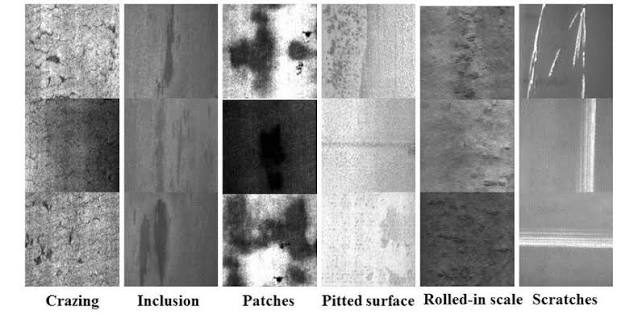
\includegraphics[width=0.8\linewidth, keepaspectratio]{img/neu_no_bbox.png}
		\caption{شش کلاس عیب در دیتاست \lr{NEU-DET}}
		\label{fig:neu_no_bbox}
	\end{figure}
	
	\subsubsection*{ویژگی‌های برچسب‌ها و چالش‌های پردازشی}
	
	برچسب‌گذاری در \lr{NEU-DET} به صورت فایل‌های متنی (\lr{xml}) با فرمت \lr{Bounding Box} ارائه شده است (شکل \ref{fig:neu_bbox}). هر تصویر ممکن است شامل یک یا چند نمونه از عیوب باشد که مختصات آن‌ها به صورت \lr{$(x_{\min}, y_{\min}, x_{\max}, y_{\max})$} ثبت شده است. مهم‌ترین چالش‌های این مجموعه داده عبارت‌اند از:
	
	\begin{enumerate}
		\item \textbf{تنوع بالای درون‌کلاسی (\lr{Intra-class Variability})}: تصاویر متعلق به یک کلاس خاص (مانند \lr{Scratches}) ممکن است به صورت افقی، عمودی یا مورب ظاهر شوند و از نظر شکل و ابعاد تفاوت‌های قابل‌توجهی داشته باشند.
		\item \textbf{شباهت بین‌کلاسی (\lr{Inter-class Similarity})}: عیوب مختلف از نظر بافت و شدت روشنایی شباهت‌های زیادی دارند که تفکیک آن‌ها حتی برای چشم انسان دشوار است.
		\item \textbf{پس‌زمینه خاکستری یکنواخت با تغییرات نوری}: تصاویر تحت شرایط کنترل‌شده ثبت شده‌اند، اما انعکاس نور روی سطح فولاد باعث تغییرات محلی در کنتراست می‌شود.
	\end{enumerate}
	
	\begin{figure}[H]
		\centering
		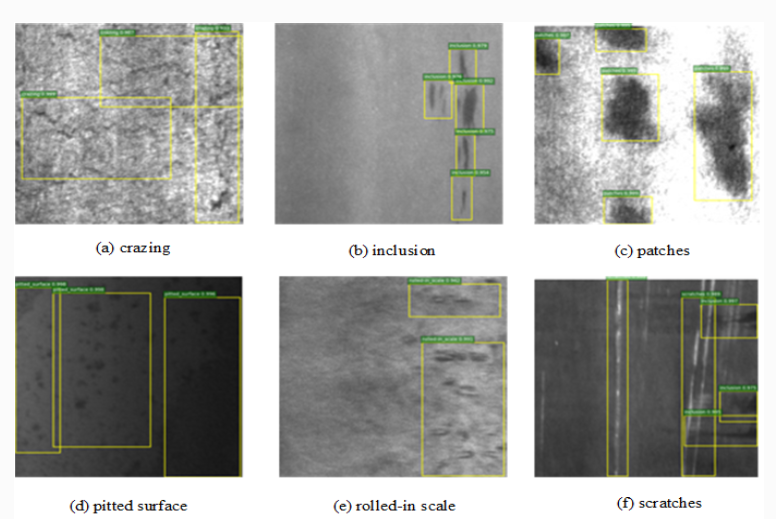
\includegraphics[width=0.8\linewidth, keepaspectratio]{img/neu_bbox.png}
		\caption{شش کلاس عیب به همراه جعبه‌های احاطه‌گر در دیتاست \lr{NEU-DET}}
		\label{fig:neu_bbox}
	\end{figure}
	
	این عیوب عیوب سطحی فولاد از نظر ابعاد و توزیع مکانی رفتار متفاوتی دارند (شکل \ref{fig:bbox_by_class}). 
	\begin{figure}[H]
		\centering
		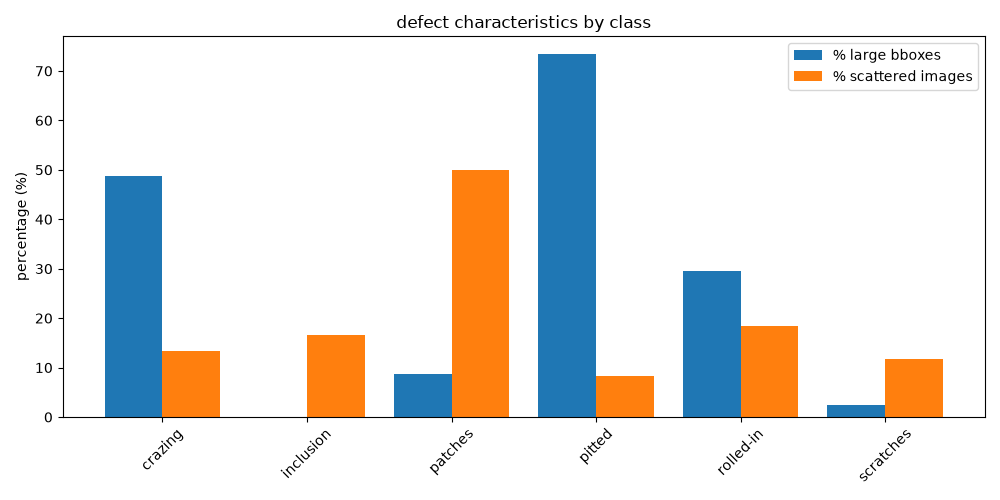
\includegraphics[width=0.8\linewidth, keepaspectratio]{img/characteristic_by_class.png}
		\caption{پراکندگی و اندازه جعبه‌های احاطه‌گر در هر کلاس عیب}
		\label{fig:bbox_by_class}
	\end{figure}
	
	به علاوه، داده‌های آماری در جدول \ref{tab:bbox_statistics} نشان می‌دهد که، کلاس سطح حفره‌دار بیشترین میزان کادرهای محاطی بزرگ ($73.3\%$) و یکی از کمترین سطوح پراکندگی ($8.3\%$) را داراست که نشان‌دهنده تمرکز عیوب در نواحی مشخص و وسیع است؛ در مقابل، کلاس وصله دقیقاً رفتار عکس را نشان داده و با داشتن بیشترین پراکندگی ($50.0\%$) و درصد پایین ابعاد بزرگ ($8.7\%$)، بیشتر به صورت توزیع‌شده و متفرق ظاهر می‌شود. همچنین نکته قابل توجه عدم وجود هرگونه کادر بزرگ در کلاس ناخالصی ($0.0\%$) است که ماهیت نقطه‌ای و موضعی این عیب را تأیید می‌کند، در حالی که کلاس ترک‌خوردگی با ترکیبی از ابعاد متوسط رو به بالا ($48.8\%$) و پراکندگی نسبی ($13.3\%$)، رفتاری بینابینی در روند تشکیل عیوب سطحی از خود نشان می‌دهد.
	
\begin{table}[H]
	\centering
	% تغییر سایز جدول به اندازه عرض ستون
	\resizebox{\columnwidth}{!}{%
		\begin{tabular}{lcc}
			\toprule
			\textbf{نام کلاس} & \textbf{کادرهای محاطی بزرگ (\%)} & \textbf{کادرهای محاطی پراکنده (\%)} \\
			& \small{(آستانه: $> 9927.00\text{ pixels}^2$)} & \small{(آستانه: $> 108.37\text{ mean pixel distance}$)} \\
			\midrule
			سطح حفره‌دار (\lr{Pitted Surface}) & $73.3\%$ & $8.3\%$ \\
			ترک‌خوردگی (Crazing) & $48.8\%$ & $13.3\%$ \\
			مقیاس نوردشده (\lr{Rolled-in Scale}) & $29.5\%$ & $18.3\%$ \\
			وصله (Patches) & $8.7\%$ & $50.0\%$ \\
			خش (Scratches) & $2.4\%$ & $11.7\%$ \\
			ناخالصی (Inclusion) & $0.0\%$ & $16.7\%$ \\
			\bottomrule
		\end{tabular}%
	}
	\caption{داده‌های آماری پراکندگی و اندازه جعبه‌های احاطه‌گر در هر کلاس عیب}
	\label{tab:bbox_statistics}
\end{table}
	محاسبه و انتخاب آستانه‌ها با توجه به صدک ۷۵ام مجموعه داده انجام شده است؛ به این صورت که تمام مساحت‌های محاسبه‌شده برای کادرهای محاطی و میانگین فواصل مکانی بین عیوب در هر تصویر مرتب‌سازی شده و نقطه‌ای که ۷۵ درصد داده‌ها زیر آن قرار می‌گیرند به عنوان آستانه تعیین شده است (شکل \ref{fig:bbox_distribution}). 
	
	\begin{figure}[H]
		\centering
		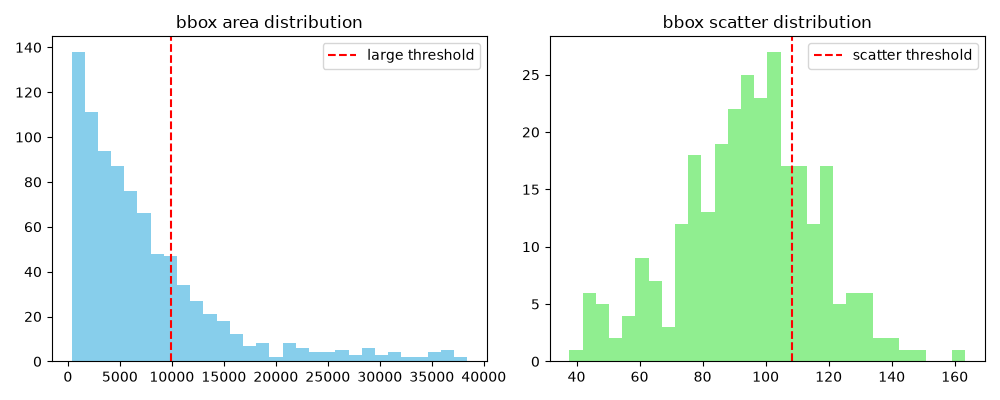
\includegraphics[width=0.8\linewidth, keepaspectratio]{img/bbox_distribution.png}
		\caption{آستانه مشخص شده برای ابعاد و پراکندگی جعبه‌های احاطه‌گر}
		\label{fig:bbox_distribution}
	\end{figure}
	
	\subsubsection*{ محدودیت عدم وجود تصاویر سالم و بدون عیب}
	
	یکی از ویژگی‌های ساختاری و در عین حال محدودیت‌های بارز مجموعه داده \lr{NEU-DET}، عدم گنجاندن تصاویر بدون عیب (\lr{Defect-Free Images}) در توزیع اولیه آن است. کلیهٔ $1800$ نمونه موجود در این بنچمارک حاوی حداقل یک نمونه از ۶ کلاس عیب سطحی بوده و هیچ‌گونه تصویر فاقد برچسب عیب در آن قرار داده نشده است. اگرچه این رویکرد تمرکز بالایی بر مسئلهٔ تشخیص عیب ایجاد می‌کند، اما با واقعیت عملیاتی خطوط تولید فولاد نورد گرم تفاوت اساسی دارد؛ زیرا در محیط صنعتی، بخش عمده‌ای از ورق‌های تولیدی فاقد هرگونه نقص هستند، بنابراین مجموعه اعتبارسنجی باید تا حد امکان بازتاب‌دهندهٔ این واقعیت باشد تا بتوان رفتار و قابلیت اطمینان مدل را در محیط عملیاتی به درستی پیش‌بینی کرد. 
	
	برای رفع این نقص بدون تغییر در فرایند آموزش مدل، تصاویر سالم صرفاً به مجموعه اعتبارسنجی (\lr{Validation}) اضافه می‌شوند. این رویکرد دو هدف کلیدی را دنبال می‌کند: نخست، امکان محاسبه نرخ مثبت کاذب (\lr{False Positive Rate}) و تنظیم دقیق آستانه اطمینان (\lr{Confidence Threshold})؛ دوم، شبیه‌سازی شرایط واقعی تست صنعتی که در آن نسبت محصولات سالم به معیوب بسیار بالاست. تصاویر سالم باید از همان دامنه آماری و بافتی دیتاست اصلی استخراج شوند تا پدیدهٔ جابجایی دامنه (\lr{Domain Shift}) رخ ندهد. علاوه بر این، حضور تصاویر سالم در اعتبارسنجی، برای تکمیل ماتریس درهم‌ریختگی (\lr{Confusion Matrix}) و محاسبهٔ معتبر شاخص‌های آماری لازم است و بدون آن، معیارهای دقت \lr{Precision}) ، \lr{FPR}، \lr{TNR}) و \lr{F1} زیر دچار نقص یا سوگیری می‌شوند.
	
	
	
	
	
	\subsection{بررسی مجموعه‌های داده جانبی جهت تأمین تصاویر سالم}
	
	\subsubsection*{مجموعه داده \lr{Severstal}}
	با توجه به ضرورت تأمین تصاویر سالم (\lr{Defect-Free}) برای تکمیل چرخهٔ اعتبارسنجی، دیتاست \lr{Severstal}  مورد بررسی قرار گرفت. علل استفاده نکردن از این دیتاست برای استخراج فریم‌های بدون ایراد به شرح زیر است:
	
	\paragraph{1. عدم تناسب دامنه‌ای (\lr{Domain Shift}): } \mbox{} \\
	
	مجموعه داده \lr{Severstal} که یکی از گزینه‌های اولیه برای استخراج تصاویر سالم بود، مربوط به فولاد نورد سرد (\lr{Cold Rolled Steel}) است. در مقابل، \lr{NEU-DET} صرفاً شامل نمونه‌های فولاد نورد گرم (\lr{Hot Rolled Steel}) می‌باشد. این تفاوت ماده‌ای و فرآیندی، منجر به اختلافات بنیادین در بافت سطحی (\lr{Surface Texture})، الگوهای نورپردازی، و ویژگی‌های طیفی تصاویر می‌شود. ادغام داده‌های نورد سرد در یک مدل آموزش‌دیده بر پایهٔ نورد گرم، پدیدهٔ جابجایی دامنهٔ شدید را به همراه دارد که باعث افت چشمگیر دقت در تشخیص عیوب و افزایش نرخ مثبت کاذب (\lr{FPR}) می‌گردد.
	
	\paragraph{2. تفاوت شدید در نسبت ابعاد (\lr{Aspect Ratio Discrepancy}): } \mbox{} \\
	
	تصاویر موجود در مجموعه \lr{Severstal} دارای ابعاد $256 \times 1600$ پیکسل هستند که نسبت ابعاد بسیار کشیده‌ای معادل تقریباً $6.25$ را ایجاد می‌کند. این در حالی است که تصاویر مرجع \lr{NEU-DET} در قالب مربعی $200 \times 200$ پیکسل ارائه شده‌اند. اعمال عملیات تغییر اندازه (\lr{Resizing}) برای انطباق ابعاد، مستلزم فشرده‌سازی شدید در یک جهت است که بافت طبیعی و الگوهای فضایی سطح فولاد نورد گرم را به‌طور کامل مخدوش می‌سازد و اطلاعات مکانی کلیدی را از بین می‌برد.
	
	\paragraph{3. عدم هم‌خوانی در ساختار برچسب‌گذاری: } \mbox{} \\
	
	ساختار برچسب‌گذاری در \lr{Severstal} بر پایه مسئله قطعه‌بندی معنایی (\lr{Semantic Segmentation}) و با استفاده از کدگذاری طول اجرای (\lr{Run-Length Encoding}) طراحی شده است. در مقابل، معماری مدل‌های مورد نظر در این پروژه بر اساس تشخیص شیء (\lr{Object Detection}) و استفاده از مستطیل‌های محدودکننده (\lr{Bounding Boxes}) بنا شده است. این ناهم‌خوانی بنیادین در سطح برچسب، امکان استفادهٔ مستقیم از ابزارها و پایپ‌لاین‌های ارزیابی موجود را سلب می‌کند.
	
	\begin{figure}[H]
		\centering
		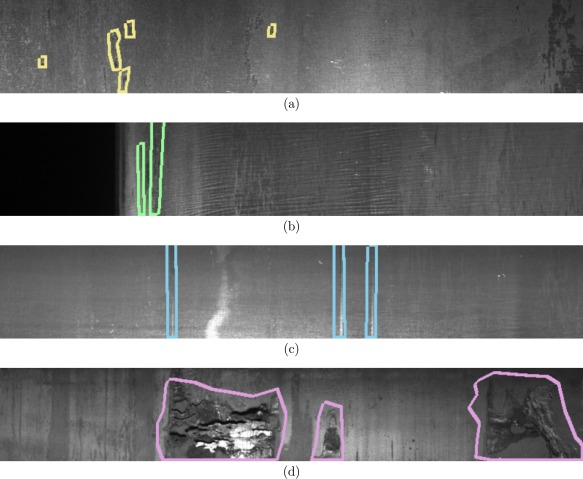
\includegraphics[width=0.8\linewidth, keepaspectratio]{img/severstal.png}
		\caption{نمونه تصاویر دیتاست \lr{severstal}}
		\label{fig:severstal}
	\end{figure}
	
	\paragraph{سایر مجموعه‌های داده بررسی‌شده: } \mbox{} \\
	علاوه بر \lr{Severstal}، دیتاست \lr{GC10-DET} و سایر دیتاست‌های موجود در \lr{NEU} نیز مورد ارزیابی قرار گرفتند، که همگی فاقد تصاویر بدون عیب بودند و از این جهت تفاوتی با مجموعه داده ابتدایی اعتبارسنجی نداشتند.
	
	\subsubsection*{نتیجه‌گیری}
	
	با توجه به ناکارآمدی منابع، رویکرد استخراج پچ‌ از پس‌زمینه بدون ایراد‌ تصاویر موجود در دیتاست (\lr{In-Domain Background Patch Extraction}) به‌عنوان راهکار جایگزین انتخاب گردید. در این روش، تصاویر سالم از نواحی پس‌زمینه خود تصاویر \lr{NEU-DET} استخراج می‌شوند؛ یعنی نواحی فاقد عیب که خارج از محدودهٔ مستطیل‌های محدودکنندهٔ ثبت‌شده قرار دارند. این روش مزایای زیر را به همراه دارد:
	
	\begin{itemize}
		\item \textbf{حفظ شرایط یکسان :} شرایط نوری، بافت فولاد و مشخصات دوربین در داده‌های آموزش و اعتبارسنجی یکسان باقی می‌ماند.
		\item \textbf{سازگاری ساختاری:} تصاویر استخراج‌شده دارای ابعاد و عمق بیت یکسان با داده‌های اصلی بوده و بدون نیاز به تغییر اندازهٔ مخرب، قابل ادغام در مجموعه اعتبارسنجی هستند.
	\end{itemize}
	
	\subsection{استخراج فریم‌های بدون عیب از مجموعه داده اصلی}
	
	\subsubsection*{مراحل الگوریتم استخراج}
	با توجه به عدم امکان استفاده از منابع برون‌دامی، فرایند استخراج فریم‌های سالم (\lr{Defect-Free Frames}) به‌طور کامل از درون خود مجموعه داده \lr{NEU-DET} صورت پذیرفت. فرآیند استخراج در شکل \ref{fig:flowchart} قابل مشاهده است و در ادامه به صورت کامل شرح داده شده است.
	\begin{figure}[H]
		\centering
		% فشرده‌سازی به اندازه عرض ستون
		\resizebox{\columnwidth}{!}{%
			\begin{tikzpicture}[
				node distance=1.8cm,
				block/.style={rectangle, draw=black, semithick, minimum width=2.8cm, minimum height=0.8cm, align=center},
				arrow/.style={-Stealth, thick}
				]
				% Nodes
				\node (step1) [block] {Binary Mask};
				\node (step2) [block, right of=step1, xshift=1.8cm] {IoU Filtering};
				\node (step3) [block, right of=step2, xshift=1.8cm] {Sliding Window};
				\node (step4) [block, right of=step3, xshift=1.8cm] {Upscale};
				\node (step5) [block, right of=step4, xshift=1.8cm] {Validation};
				
				% Arrows
				\draw [arrow] (step1) -- (step2);
				\draw [arrow] (step2) -- (step3);
				\draw [arrow] (step3) -- (step4);
				\draw [arrow] (step4) -- (step5);
			\end{tikzpicture}%
		}
		\caption{مراحل الگوریتم استخراج}
		\label{fig:flowchart}
	\end{figure}
	
	\paragraph{۱. تحلیل و ماسک‌گذاری کادرهای عیب (\lr{Binary Mask Generation}): }
	
	در گام نخست، فایل‌های برچسب (\lr{txt}) متناظر با هر تصویر خوانده شده و مختصات مستطیل‌های محدودکنندهٔ عیوب (\lr{$x_{\min}, y_{\min}, x_{\max}, y_{\max}$}) استخراج گردید. بر اساس این مختصات، یک ماسک دودویی (\lr{Binary Mask}) با ابعاد برابر تصویر اصلی ($200 \times 200$) تولید شد که در آن پیکسل‌های متعلق به نواحی عیب مقدار $1$ (ناحیهٔ معیوب) و سایر نواحی مقدار $0$ (ناحیهٔ سالم/پس‌زمینه) را به خود گرفتند.
	
	\paragraph{۲. انتخاب ناحیهٔ غیرهم‌پوشان (\lr{Non-Overlapping Region Selection}): }
	
	برای جلوگیری از نشت داده و اطمینان از خلوص فریم‌های استخراج‌شده، نواحی سالم باید کاملاً خارج از محدودهٔ عیوب قرار گیرند. به این منظور، معیار \lr{Intersection over Union} (\lr{IoU}) به کار گرفته شد؛ به‌طوری‌که تنها نواحی با $\text{\lr{IoU}} = 0$ نسبت به کادرهای عیب به عنوان کاندیدای نهایی پذیرفته شدند. این شرط تضمین می‌کند که هیچ‌گونه پیکسل متعلق به عیب در فریم استخراج‌شده باقی نماند.
	
	\paragraph{۳. اعمال پنجرهٔ لغزان (\lr{Sliding Window Extraction}): }
	
	برای استخراج پچ‌های مربعی یکنواخت از نواحی سالم، الگوریتم پنجرهٔ لغزان با پارامترهای زیر به کار گرفته شد:
	
\begin{table}[H]
	\centering
	% فشرده‌سازی جدول به اندازه عرض یک ستون
	\resizebox{\columnwidth}{!}{%
		\begin{tabular}{ccc}
			\toprule
			پارامتر & مقدار & توضیحات فنی \\
			\midrule
			ابعاد پنجره (\lr{Window Size}) & $100 \times 100$ & ابعاد اولیهٔ استخراج بر حسب پیکسل \\
			گام حرکتی (\lr{Stride}) & $10$ & میزان تغییر مکان پنجره در هر گام \\
			معیار پذیرش هم‌پوشانی & $\text{\lr{IoU}} = 0$ & عدم تداخل با هیچ‌یک از \lr{Bounding Box}های عیب \\
			\bottomrule
		\end{tabular}%
	}
	\caption{پارامترهای عملیاتی الگوریتم پنجرهٔ لغزان}
	\label{tab:sliding-window-params}
\end{table}
	
	انتخاب ابعاد $100 \times 100$ به جای $200 \times 200$ در گام اول، امکان استخراج چندین نمونه سالم از یک تصویر واحد را فراهم می‌سازد؛ در حالی که گام $10$ پیکسلی تضمین می‌کند نواحی سالم با تنوع بافتی کافی پوشش داده شوند.
	
	شکل \ref{fig:background} چند نمونه از پچ‌های استخراج شده با پنجره لغزان (رنگ سبز) و جعبه‌ احاطه‌گر (رنگ قرمز) را روی تصاویر اصلی نشان می‌دهد.
	\begin{figure}[H]
		\centering
		
		\begin{subfigure}[b]{0.23\linewidth}
			\centering
			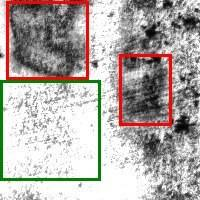
\includegraphics[width=\linewidth]{img/1.jpg}
			\caption{}
		\end{subfigure}
		\hfill
		\begin{subfigure}[b]{0.23\linewidth}
			\centering
			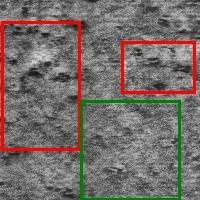
\includegraphics[width=\linewidth]{img/2.jpg}
			\caption{}
		\end{subfigure}
		\hfill
		\begin{subfigure}[b]{0.23\linewidth}
			\centering
			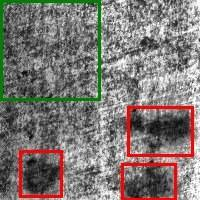
\includegraphics[width=\linewidth]{img/3.jpg}
			\caption{}
		\end{subfigure}
		\hfill
		\begin{subfigure}[b]{0.23\linewidth}
			\centering
			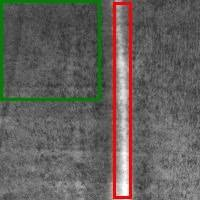
\includegraphics[width=\linewidth]{img/4.jpg}
			\caption{}
		\end{subfigure}
		
		\caption{نمونه جعبه‌های احاطه‌گر ایراد و پچ‌های انتخاب شده}
		\label{fig:background}
	\end{figure}
	
	
	\paragraph{۴. تغییر مقیاس به ابعاد استاندارد (\lr{Upscale})}
	
	پچ‌های استخراج‌شده با ابعاد $100 \times100$ پیکسل، در مرحلهٔ نهایی به ابعاد استاندارد $200 \times 200$ پیکسل ارتقا یافتند. این عملیات تغییر مقیاس (\lr{Upscale}) با استفاده از درونیابی هم‌بافت (\lr{Bicubic Interpolation}) انجام شد تا ضمن حفظ جزئیات بافتی، سازگاری ابعادی با دیتاست اصلی \lr{NEU-DET} برقرار گردد.
	
	چند نمونه از تصاویر استخراج شده پس از تغییر مقیاس در شکل \ref{fig:extracted} قابل مشاهده است.
	\begin{figure}[H]
		\centering
		% اعمال resizebox برای فشرده‌سازی کل مجموعه در یک ستون
		\resizebox{\columnwidth}{!}{%
			\begin{minipage}{\textwidth} % ایجاد یک بستر موقت برای چیدمان
				\begin{subfigure}[b]{0.23\linewidth}
					\centering
					
\includegraphics[width=\linewidth]{img/clean_379.jpg}
					\caption{}
				\end{subfigure}
				\hfill
				\begin{subfigure}[b]{0.23\linewidth}
					\centering
					
\includegraphics[width=\linewidth]{img/clean_571.jpg}
					\caption{}
				\end{subfigure}
				\hfill
				\begin{subfigure}[b]{0.23\linewidth}
					\centering
					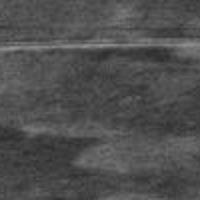
\includegraphics[width=\linewidth]{img/clean_1649.jpg}
					\caption{}
				\end{subfigure}
				\hfill
				\begin{subfigure}[b]{0.23\linewidth}
					\centering
					
\includegraphics[width=\linewidth]{img/clean_2858.jpg}
					\caption{}
				\end{subfigure}
			\end{minipage}%
		}
		\caption{نمونه تصاویر استخراج شده پس از تغییر مقیاس}
		\label{fig:extracted}
	\end{figure}
	
	\subsection{تحلیل آماری و دیداری فریم‌ها پیش از ترکیب با مجموعه داده اصلی}
	
	\subsubsection*{سنجش ویژگی‌های آماری و هیستوگرام شدت روشنایی}
	
	پیش از ادغام فریم‌های استخراج‌شده در مجموعه اعتبارسنجی، تحلیل آماری بر پایهٔ شاخص‌های شدت روشنایی (\lr{Mean Intensity})، انحراف معیار (\lr{Standard Deviation}) و هیستوگرام توزیع شدت پیکسل (\lr{Pixel Intensity Histogram}) انجام گرفت. هدف از این تحلیل، اطمینان از انطباق آماری و جلوگیری از افت کیفیت مدل پس از ترکیب بود. لازم به ذکر است که تصاویر استخراج‌شده با پس‌زمینه تصاویر اصلی اعتبارسنجی مقایسه شده‌اند.
	
	نتایج کمی در جداول \ref{tab:stat1} و \ref{tab:stat2} ارائه شده‌اند.
	
	\begin{table}[H]
		\centering
		\resizebox{\columnwidth}{!}{
		\begin{tabular}{ccc}
			\toprule
			مجموعه داده & میانگین شدت روشنایی (\lr{Mean}) & انحراف معیار (\lr{Std Dev}) \\
			\midrule
			پس‌زمینه اعتبارسنجی (\lr{Validation - BG Only}) & $131.89$ & $34.88$ \\
			فریم‌های استخراج‌شده (\lr{Extracted Dataset}) & $106.94$ & $17.38$ \\
			قدر مطلق انحراف (\lr{Absolute Deviation}) & $\Delta = 24.95$ & $\Delta = 17.50$ \\
			\bottomrule
		\end{tabular}
		}
		\caption{مقایسه شاخص‌های روشنایی و کنتراست میان پس‌زمینه اعتبارسنجی و فریم‌های استخراج‌شده}
		\label{tab:stat1}
	\end{table}
	
	\begin{table}[H]
		\centering
			\resizebox{\columnwidth}{!}{
		\begin{tabular}{ccccc}
			\toprule
			مجموعه داده & قله هیستوگرام (\lr{Peak Bin}) & تیره ($0$-$84$) & میانی ($85$-$169$) & روشن ($170$-$255$) \\
			\midrule
			پس‌زمینه اعتبارسنجی & $255$ & $20.2\%$ & $55.7\%$ & $24.1\%$ \\
			فریم‌های استخراج‌شده & $83$ & $34.1\%$ & $56.9\%$ & $8.9\%$ \\
			\bottomrule
		\end{tabular}
		}
		\caption{مقایسه درصد توزیع پیکسل‌ها و قله هیستوگرام در بازه‌های مختلف}
		\label{tab:stat2}
	\end{table}
	
	نمودارهای مقایسه شاخص‌های روشنایی و کنتراست به همراه نمودار هیستوگرام در شکل \ref{fig:comp_res} قابل مشاهده هستند.
	\begin{figure}[H]
		\centering
		
\includegraphics[width=0.8\linewidth, keepaspectratio]{img/results.png}
		\caption{مقایسه روشنایی و کنتراست و نمودار هیستوگرام بین پس‌زمینه داده‌های اصلی و فریم‌های استخراج‌شده}
		\label{fig:comp_res}
	\end{figure}
	
	
	\subsubsection*{تحلیل تفاوت‌های آماری و بافتی}
	
	نتایج جدول \ref{tab:stat1} نشان‌دهندهٔ اختلاف $24.95$ واحدی در میانگین شدت روشنایی و $17.50$ واحدی در انحراف معیار است. دلیل اصلی این اختلاف به ماهیت فیزیکی نمونه‌ها مربوط می‌شود:
	
	\begin{itemize}
		\item \textbf{تفاوت در قلهٔ هیستوگرام:}
		پس‌زمینهٔ اعتبارسنجی دارای قلهٔ شدت در بازهٔ $255$ (سفید مطلق) است؛ زیرا این ناحیه اغلب شامل نواحی پس‌زمینهٔ روشن و اشباع‌شده خارج از بافت اصلی فولاد می‌باشد. در مقابل، فریم‌های استخراج‌شده دارای قلهٔ $83$ هستند که نمایندهٔ بافت واقعی سطح فولاد نورد گرم با تیرگی طبیعی است.
		\item \textbf{هم‌گرایی در بازهٔ میانی:}
		آنچه اهمیت ساختاری دارد، هم‌پوشانی بالای دو مجموعه در بازهٔ میانی ($85$-$169$) است. پس‌زمینه اعتبارسنجی $55.7\%$ و فریم‌های استخراج‌شده $56.9\%$ از پیکسل‌ها را در این بازه دارند. این هم‌گرایی بیانگر آن است که بافت اصلی هر دو مجموعه از یک توزیع آماری پیروی می‌کند.
		\item \textbf{یکنواختی بافت استخراج‌شده:} 
		انحراف معیار پایین‌تر فریم‌های استخراج‌شده ($17.38$ در مقابل $34.88$) نشان می‌دهد که این نمونه‌ها از یکنواختی بالاتری برخوردارند.
	\end{itemize}
	
	\paragraph{نتیجه‌گیری} \mbox{} \\
	
	با وجود اختلاف ظاهری در میانگین شدت روشنایی و قلهٔ هیستوگرام، فریم‌های استخراج‌شده برای ادغام با مجموعه داده اصلی کاملاً مناسب‌اند. دلایل فنی این ادعا به شرح زیر است:
	
	\begin{enumerate}
		\item \textbf{هم‌خوانی ماده‌ای و فرایندی:}
		هر دو مجموعه متعلق به فولاد نورد گرم هستند؛ بنابراین پدیدهٔ جابجایی دامنه که مهم‌ترین مانع در استفاده از داده‌های برون‌دامی (نظیر \lr{Severstal}) بود، در اینجا رخ نمی‌دهد.
		\item \textbf{اصلاح توزیع آماری اعتبارسنجی:}
		فریم‌های استخراج‌شده با حذف پیکسل‌های اشباع‌شدهٔ پس‌زمینه (قلهٔ $255$)، توزیع واقعی‌تری از بافت سطح فولاد را به مجموعه اعتبارسنجی تزریق می‌کنند. این امر باعث می‌شود مدل به جای یادگیری تفاوت‌های نوری مصنوعی، ویژگی‌های ساختاری عیوب را فرا گیرد.
		\item \textbf{امکان سنجش معتبر \lr{FPR}:}
		ادغام این فریم‌ها بدون ایجاد انحراف دامنه‌ای، امکان محاسبهٔ نرخ مثبت کاذب و سایر معیارهای وابسته به کلاس سالم (\lr{Specificity}، \lr{Precision}، \lr{AUC-ROC}) را در مجموعه اعتبارسنجی فراهم می‌سازد.
	\end{enumerate}
	
	\subsection{آماده‌سازی داده‌ها برای شبیه‌سازی سناریوهای کارخانه در \lr{Webots}}
	
	پس از تفکیک داده‌های اعتبارسنجی و استخراج فریم‌های سالم، نوبت به تولید توالی‌های زمانی (\lr{Temporal Sequences}) می‌رسد که رفتار واقعی یک خط تولید فولاد را در محیط شبیه‌ساز \lr{Webots} بازسازی کنند. در این راستا، سه روش متوالی و رو به رشد در پیچیدگی طراحی شد: روش اول مبتنی بر زنجیرهٔ مارکوف ساده، روش دوم با تلفیق ماشین حالت محدود، و روش سوم بر پایهٔ مدل سلامت ماشین (\lr{Asset Health}) که به‌عنوان راهکار نهایی انتخاب گردید.
	
	\subsubsection*{روش اول: ادغام بر پایهٔ زنجیرهٔ مارکوف (\lr{Markov Chain Merging})}
	
	این روش با هدف ایجاد توالی‌هایی از فریم‌ها با رعایت احتمالات انتقال واقعی بین حالت‌های سالم و معیوب، یک مدل احتمالاتی گسسته در زمان (\lr{Discrete-Time Markov Chain}) را پیاده‌سازی می‌کند.
	
	\paragraph{تعریف فضای حالت (\lr{State Space}): }\mbox{} \\
	
	فضای حالت سیستم به صورت مجموعهٔ متناهی زیر تعریف می‌شود:
	
	$$S = \{S_0, S_1, S_2, \ldots, S_k\}$$
	
	که در آن $S_0$ نمایندهٔ حالت «فریم سالم» (\lr{Defect-Free}) و هر یک از $S_1$ تا $S_k$ نمایندهٔ یکی از کلاس‌های عیب متفاوت (مانند \lr{Crazing}، \lr{Pitted}، \lr{Patches} و غیره) هستند.
	
	\paragraph{تشکیل ماتریس احتمال انتقال (\lr{Transition Probability Matrix}): } \mbox{} \\
	
	ماتریس انتقال $P$ یک ماتریس مربعی به ابعاد $(k+1) \times (k+1)$ است که درایهٔ $p_{ij}$ بیانگر احتمال انتقال از حالت $S_i$ در گام $n$ به حالت $S_j$ در گام $n+1$ می‌باشد:
	
	$$P = \begin{bmatrix} p_{00} & p_{01} & \cdots & p_{0k} \\ p_{10} & p_{11} & \cdots & p_{1k} \\ \vdots & \vdots & \ddots & \vdots \\ p_{k0} & p_{k1} & \cdots & p_{kk} \end{bmatrix} $$
	
	$$p_{ij} = P(X_{n+1} = S_j \mid X_n = S_i)$$
	
	\paragraph{محاسبهٔ ماتریس انتقال $P$: }\mbox{} \\
	
	برای تخمین ماتریس $P$ از روی داده‌های تجربی مجموعه اعتبارسنجی، از روش بیشینه درست‌نمایی (\lr{Maximum Likelihood Estimation}) استفاده می‌شود:
	
	\begin{enumerate}
		\item \textbf{شمارش فراوانی گذارها:} ماتریس شمارش $C$ به ابعاد $(k+1) \times (k+1)$ تشکیل می‌شود که درایهٔ $C_{ij}$ برابر تعداد دفعات مشاهدهٔ گذار از $S_i$ به $S_j$ در توالی داده‌های آموزشی است:
		$$C_{ij} = \text{Count}(X_{n+1} = S_j \mid X_n = S_i)$$
		
		\item \textbf{نرمال‌سازی سطری (\lr{Row-wise Normalization}):} برای تبدیل شمارش‌ها به احتمال شرطی، هر سطر $i$ ام بر مجموع عناصر همان سطر تقسیم می‌شود:
		$$p_{ij} = \frac{C_{ij}}{\sum_{m=0}^{k} C_{im}} $$
		این عملیات تضمین می‌کند که ماتریس $P$ یک ماتریس تصادفی سطری (\lr{Row-stochastic Matrix}) باشد؛ به‌طوری‌که $\sum_{j=0}^{k} p_{ij} = 1$.
		
		\item \textbf{هموارسازی لاپلاس (\lr{Laplace / Add-1 Smoothing}):} برای جلوگیری از صفر شدن احتمالات گذارهای نادر و وقوع حالت‌های بی‌نتیجه در شبیه‌ساز \lr{Webots}، یک پارامتر کوچک $\epsilon > 0$ به تمام شمارش‌ها اضافه می‌شود:
		$$p_{ij} = \frac{C_{ij} + \epsilon}{\sum_{m=0}^{k} (C_{im} + \epsilon)} $$
		این هموارسازی به‌ویژه برای حالاتی که $C_{ii} = 0$ باشد، اهمیت حیاتی دارد.
	\end{enumerate}
	
	
	\subsubsection*{روش دوم: زنجیرهٔ مارکوف به همراه ماشین حالت (\lr{Markov Chain + State Machine})}
	
	این روش با افزودن لایهٔ ماشین حالت محدود (\lr{Finite State Machine})، رفتار زنجیرهٔ مارکوف را از حالت حافظه‌less (\lr{Memoryless}) به ساختاری هدایت‌شده با حافظهٔ کوتاه‌مدت ارتقا می‌دهد.
	
	\paragraph{تعریف ساختار ماشین حالت محدود (\lr{FSM}): } \mbox{} \\
	
	ماشین حالت (شکل \ref{fig:statemachine} شامل چهار حالت عملیاتی کارخانه است:
	
	$$M = \{M_{\text{Normal}}, M_{\text{Degrading}}, M_{\text{Critical}}, M_{\text{Recovery}}$$
	
	\begin{itemize}
		\item $M_{\text{Normal}}$: حالت کارکرد عادی خط تولید (تولید ورق سالم با عیوب بسیار نادر).
		\item $M_{\text{Degrading}}$: حالت استهلاک تدریجی (افزایش احتمال بروز عیوب سطحی و متوسط).
		\item $M_{\text{Critical}}$: حالت بحرانی (تولید مدادوم عیوب ساختاری و بزرگ).
		\item $M_{\text{Recovery}}$: حالت بازیاپی و تنظیم مجدد دستگاه‌ها پس از رفع مشکل.
	\end{itemize}
	
	\begin{figure}[H]
		\centering
		\resizebox{\columnwidth}{!}{
		\begin{tikzpicture}[
			->, >=Stealth, node distance=3.5cm, every state/.style={draw=black, semithick, fill=gray!10},
			initial text=
			]
			% Nodes (States)
			\node[state, initial] (normal) {$M_{\text{Normal}}$};
			\node[state, right of=normal] (degrading) {$M_{\text{Degrading}}$};
			\node[state, below of=degrading] (critical) {$M_{\text{Critical}}$};
			\node[state, left of=critical] (recovery) {$M_{\text{Recovery}}$};
			
			% Transitions (Edges)
			\path[every node/.style={font=\small}]
			% Self-loops
			(normal) edge[loop above] node {\rl{کارکرد عادی}} (normal)
			(degrading) edge[loop above] node {\rl{افزایش استهلاک}} (degrading)
			(critical) edge[loop right] node {\rl{تولید عیب مداوم}} (critical)
			
			% Forward transitions
			(normal) edge[above] node {\rl{شروع استهلاک}} (degrading)
			(degrading) edge[right] node {\rl{ورود به شرایط بحرانی}} (critical)
			(critical) edge[below] node {\rl{توقف و توقف خط}} (recovery)
			(recovery) edge[left] node {\rl{تنظیم مجدد}} (normal)
			
			% Direct emergency / recovery paths
			(degrading) edge[above left] node {\rl{تنظیم سریع}} (recovery);
		\end{tikzpicture}
		}
		\caption{دیاگرام ماشین حالت $M$ برای گام‌های عملیاتی خط تولید فولاد}
		\label{fig:statemachine}
	\end{figure}
	
	\paragraph{تلفیق ماتریس انتقال مارکوف با حالات ماشین (\lr{FSM-Guided Transition}): } \mbox{} \\
	
	در این روش، ماتریس انتقال پایهٔ $P$ تحت تأثیر حالت جاری ماشین $M_n$ قرار می‌گیرد. برای هر حالت $M_k \in M$، یک ماتریس انتقال شرطی $P^{(M_k)}$ تعریف می‌شود:
	
	$$P(M_n) = f(P_{\text{base}}, M_n)$$
	
	$$p_{ij}^{(M_k)} = P(X_{n+1} = S_j \mid X_n = S_i, M_n = M_k) $$
	
	قواعد انتقال بین حالات ماشین بر اساس تعداد عیب‌های شناسایی‌شده در پنجرهٔ زمانی اخیر ($N_{\text{defect}}$) و آستانه‌های $T_1$ و $T_2$ به صورت زیر تعریف می‌شود:
	
	\begin{equation*} % جایگزین $$ برای اعمال درست تغییر سایز
		\resizebox{\columnwidth}{!}{%
			$\displaystyle
			M_{n+1} = 
			\begin{cases}
				M_{\text{Degrading}} & \text{if } M_n = M_{\text{Normal}} \text{ and } N_{\text{defect}} \geq T_1 \\
				M_{\text{Critical}} & \text{if } M_n = M_{\text{Degrading}} \text{ and } N_{\text{defect}} \geq T_2 \\
				M_{\text{Recovery}} & \text{if } M_n = M_{\text{Critical}} \text{ and } N_{\text{maintenance}} \text{ triggered} \\
				M_{\text{Normal}} & \text{if } M_n = M_{\text{Recovery}} \text{ and reset completed}
			\end{cases}
			$%
		}
	\end{equation*}
	
	
	\subsubsection*{روش سوم: مدل مبتنی بر شاخص سلامت (\lr{Full Health-Based Model})}
	
	این روش پیشرفته‌ترین سطح مدل‌سازی را ارائه می‌دهد که در آن، ظهور عیوب نه یک پدیدهٔ تصادفی مستقل، بلکه تابعی از فرسایش تدریجی و استهلاک ماشین‌آلات خط نورد است.
	
	\paragraph{مدل‌سازی دینامیک استهلاک و شاخص سلامت (\lr{Health Indicator Dynamics})} \mbox{} \\
	
	شاخص سلامت $H(t) \in [0, 1]$ در زمان $t$ بیانگر میزان سلامت تجهیزات است. مقدار $H(t) = 1$ نشان‌دهندهٔ سلامت کامل و $H(t) \to 0$ نشان‌دهندهٔ تخریب کامل تجهیزات است. مدل تخریب به صورت تصادفی (\lr{Stochastic Degradation Model}) تعریف می‌شود:
	
	$$H(t + \Delta t) = H(t) - \Delta H_t$$
	
	که در آن نرخ افت سلامت $\Delta H_t$ از یک توزیع نرمال یک‌طرفه (\lr{Half-normal} یا \lr{Truncated Normal}) پیروی می‌کند:
	
	$$\Delta H_t \sim \mathcal{N}^{+}(\mu_d, \sigma_d^2) $$
	
	این مدل‌سازی، نوسانات محیطی واقعی کارخانه (تغییرات دما، لرزش، بار مکانیکی) را در قالب یک فرایند تصادفی لحاظ می‌کند.
	
	\paragraph{نگاشت احتمالی شاخص سلامت به توزیع عیوب (\lr{Health-to-Defect Mapping})} \mbox{} \\
	
	برای تبدیل مقدار سلامت جاری $H(t)$ به توزیع احتمال کلاس‌های عیب، از تابع \lr{Weighted Softmax} با وزن‌دهی گوسی استفاده می‌شود:
	
	$$P(X_t = S_k \mid H(t)) = \frac{\exp\left(-\frac{(H(t) - \mu_k)^2}{2\sigma_k^2}\right)}{\sum_{m=0}^{K} \exp\left(-\frac{(H(t) - \mu_m)^2}{2\sigma_m^2}\right)} $$
	
	پارامترهای مرکز $\mu_k$ و پراکندگی $\sigma_k$ برای هر کلاس عیب به صورت تجربی تنظیم می‌شوند:
	
	\begin{itemize}
		\item $\mu_0 = 1.0$: نقطهٔ اوج شاخص سلامت برای فریم سالم (\lr{Defect-Free}).
		\item $\mu_{\text{pitted}} = 0.7$: عیب خفیف‌تر با مرکزیت بالاتر.
		\item $\mu_{\text{crazing}} = 0.2$: عیب شدیدتر با مرکزیت نزدیک به صفر.
		\item $\sigma_k$: بیانگر گسترهٔ احتمالی بروز عیب در اطراف نقطهٔ اوج است.
	\end{itemize}
	
	
	\subsubsection*{تحلیل و مقایسه روش‌ها و نمودارها}
	
	\begin{table}[htbp]
		\centering
		\resizebox{\columnwidth}{!}{
		\begin{tabular}{ccccc}
			\toprule
			معیار ارزیابی & روش اول (\lr{Markov}) & روش دوم (\lr{Markov+FSM}) & روش سوم (\lr{Health-Based}) \\
			\midrule
			طبیعت متغیر وضعیت & گسسته & گسسته + چندسطحی & پیوسته \\
			واقع‌گرایی فیزیکی & پایین (جهش‌های آنی) & متوسط (حالات پله‌ای) & بالا (استهلاک نرم و تدریجی) \\
			تغییر ابعاد عیوب & ثابت & ثابت / پله‌ای & پیوسته و متناسب با $(1-H(t))$ \\
			وابستگی به ماتریس انتقال $P$ & کامل & نسبی (تعدیل‌شده توسط \lr{FSM}) & مبتنی بر تابع سلامت پیوسته \\
			حساسیت پارامتری & بالا (تنظیم آستانه‌ها) & بالا ($T_1, T_2$) & متوسط ($\mu_d, \sigma_d$) \\
			ارزیابی چرخه عمر & غیرممکن & محدود به حالات گسسته & کامل (از سلامت $100\%$ تا تخریب کامل) \\
			\bottomrule
		\end{tabular}
	}
		\caption{مقایسه روش‌های تولید توالی داده در خط تولید}
		\label{tab:method-comparison}
	\end{table}
	
	نمودار چگالی عیوب در شکل \ref{fig:defectDensity} نشان می‌دهد که مدل \lr{Markov} دچار نوسانات شدید و اسپایک‌های لحظه‌ای پراکنده در طول فریم‌هاست؛ در مقابل، مدل \lr{Refined} این نوسانات را تا حدی هموار کرده اما همچنان ساختاری گسسته دارد، و مدل \lr{HealthModel} با ایجاد قله‌های منحنی و پیوسته در فریم‌های بحرانی (مانند فریم $800$ و $1700$)، روند تدریجی پدیدار شدن و رفع عیوب را به بهترین شکل بازنمایی می‌کند.
	\begin{figure}[H]
		\centering
		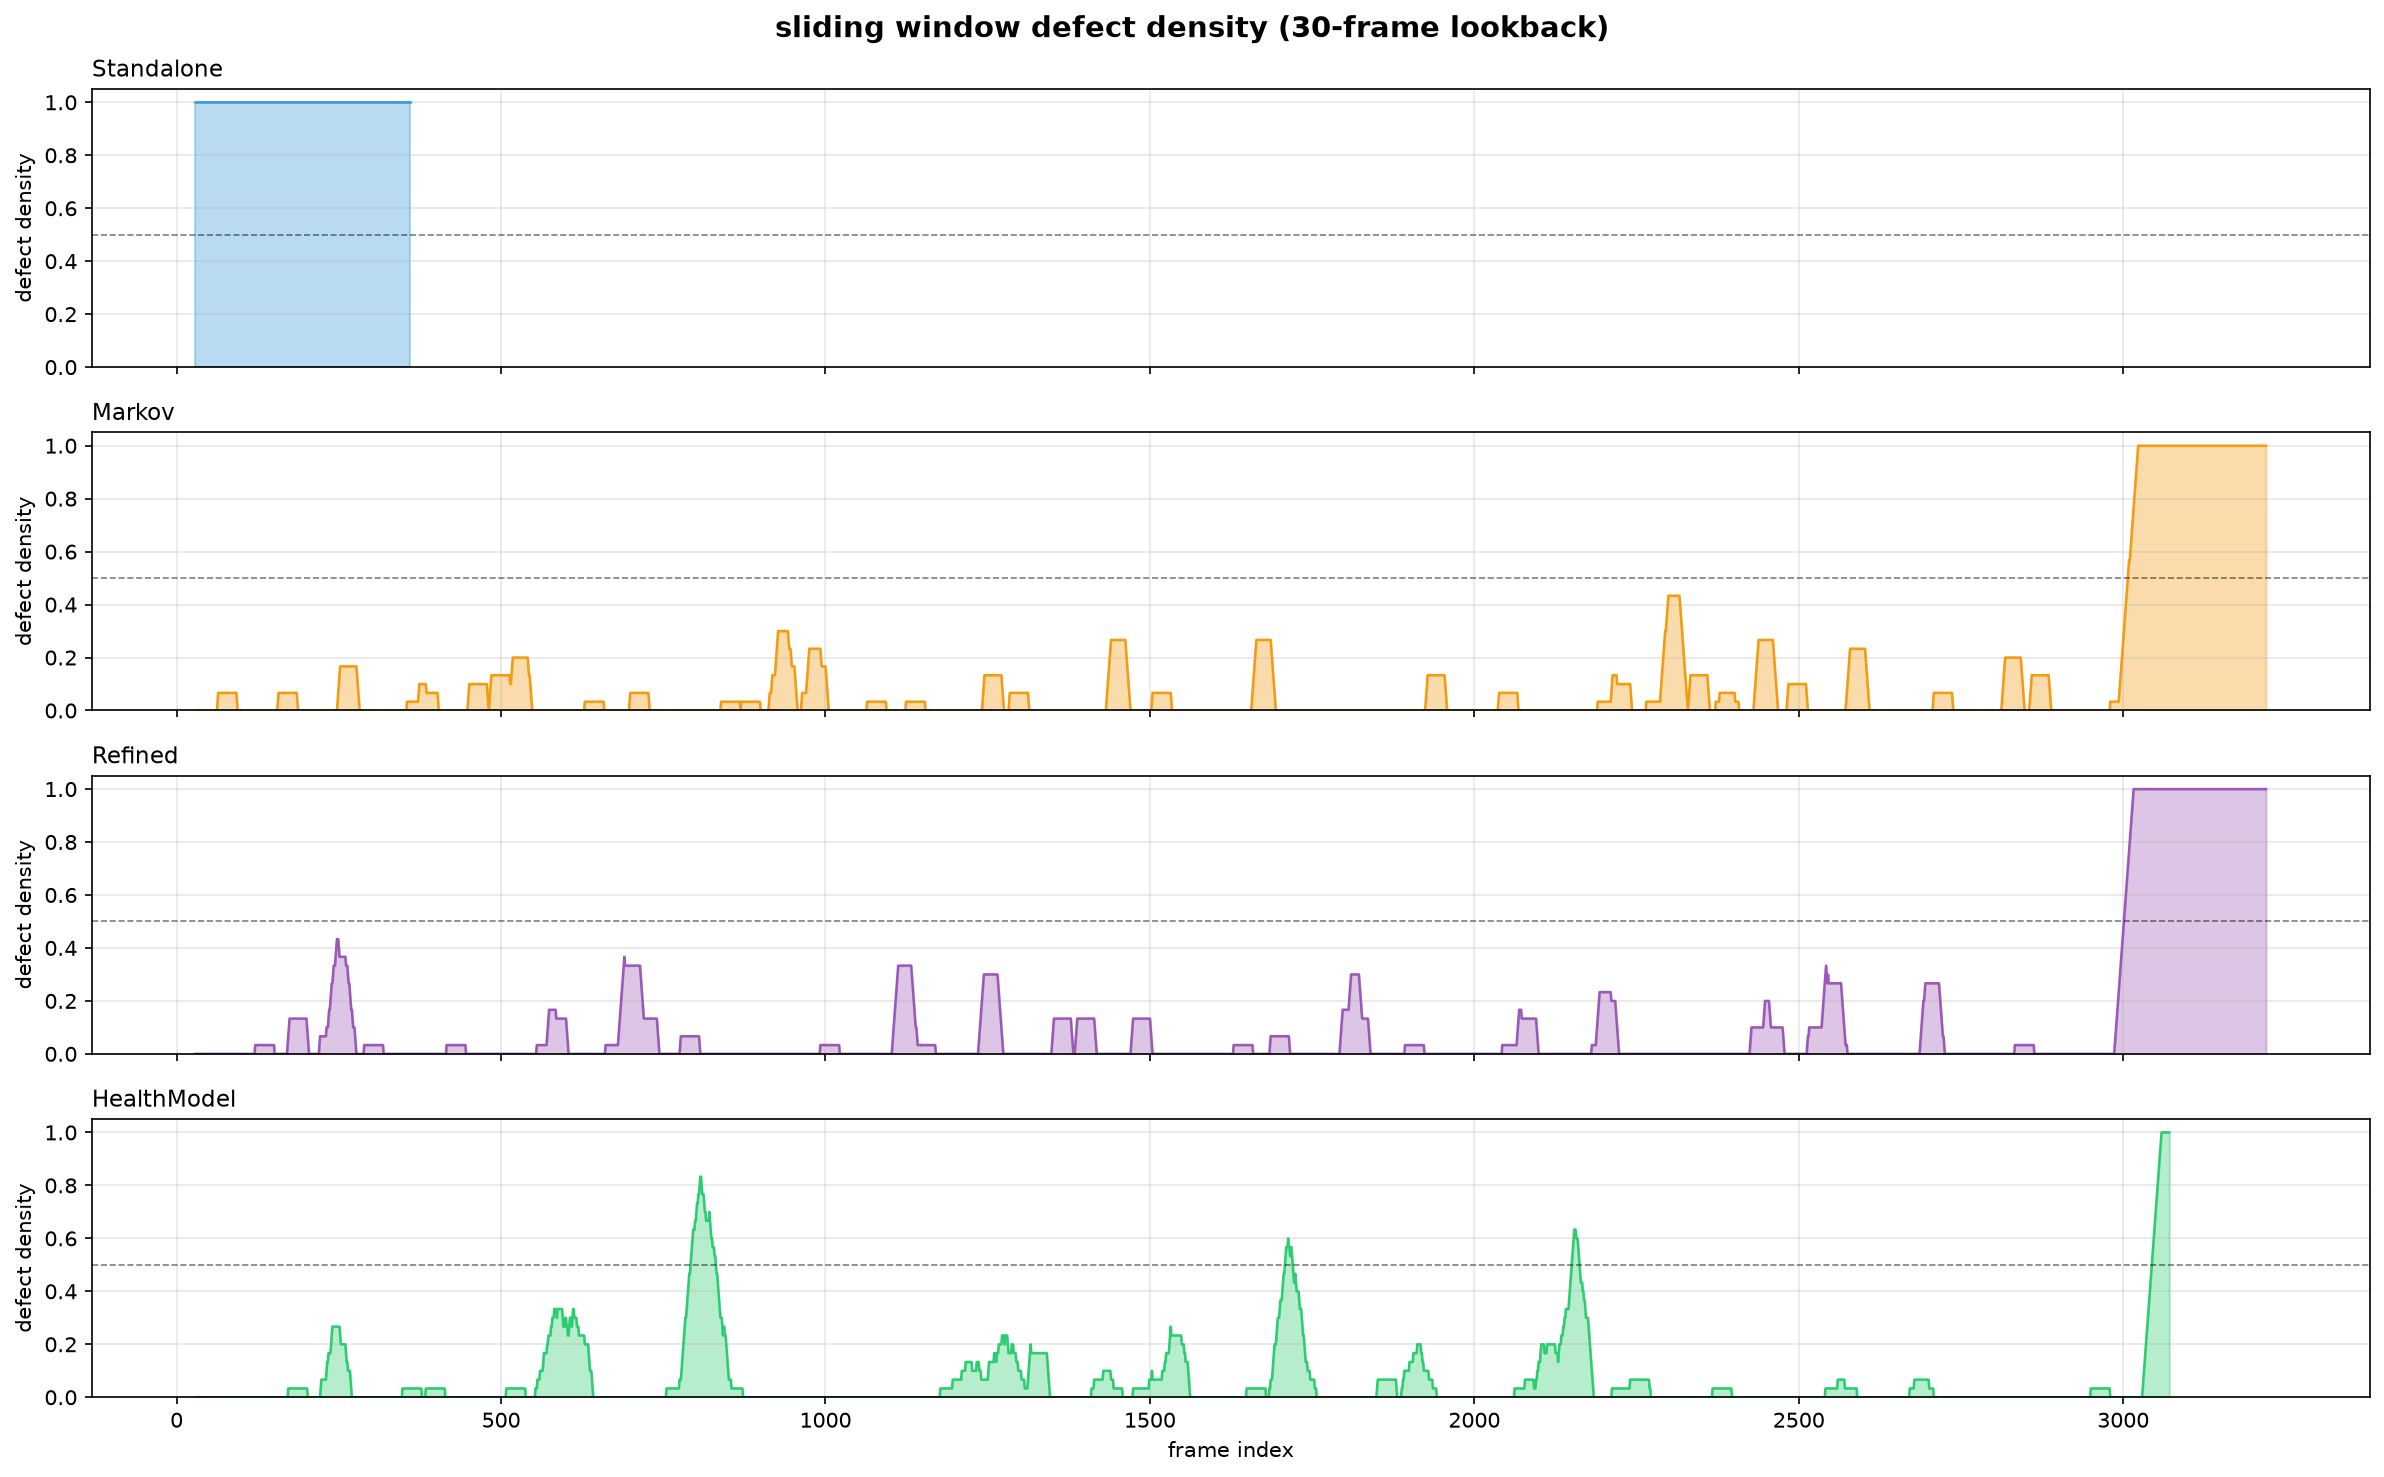
\includegraphics[width=0.8\linewidth, keepaspectratio]{img/defectDensity.png}
		\caption{چگالی عیوب در طول زمان (30 فریم)}
		\label{fig:defectDensity}
	\end{figure}
	
	در شکل \ref{fig:runLength} که توزیع طول بازه تداوم عیوب را بررسی می‌کند، مدل \lr{Markov} افت فوق‌العاده شدیدی را در طول بازه نشان می‌دهد که گواهی بر عدم ثبات و پدیده پرش لحظه‌ای آن است؛ مدل \lr{Refined} تداوم‌های بسیار طولانی‌تری (تا $50$ یا $60$ فریم متوالی) را ثبت کرده که پایداری بالا اما گاه غیرعادی را نشان می‌دهد، و مدل \lr{HealthModel} با شیب نزولی متعادل، رفتاری مابین دو مدل دیگر ارائه داده و تداوم زمانی منطقی عیوب را بدون قفل شدن روی یک حالت خاص حفظ می‌کند.
	\begin{figure}[H]
		\centering
		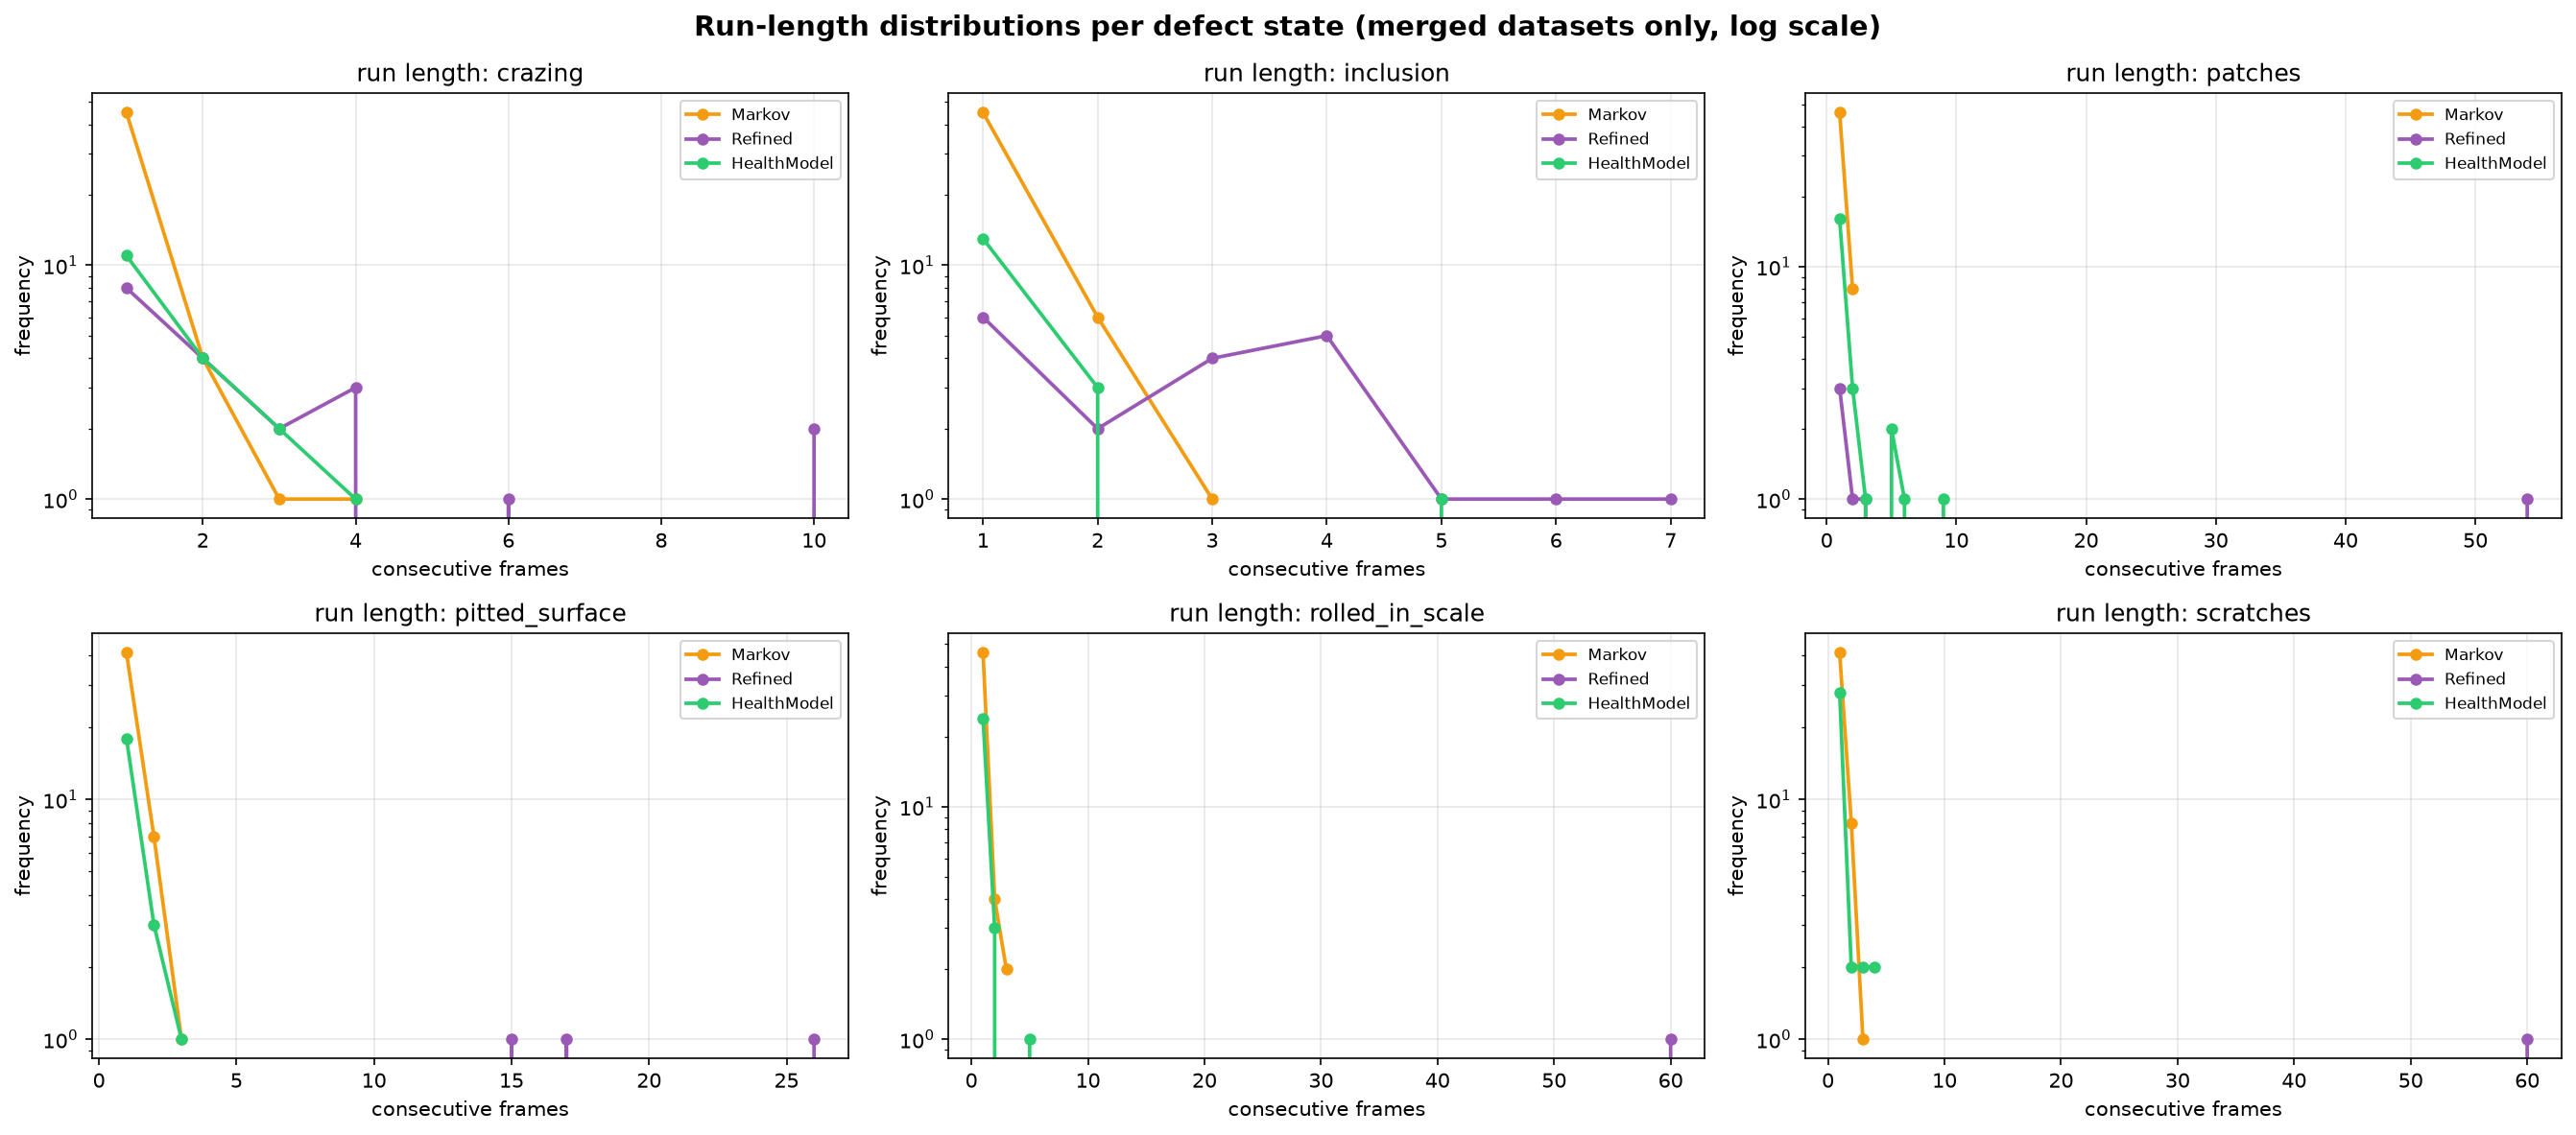
\includegraphics[width=0.8\linewidth, keepaspectratio]{img/runLength_distribution.png}
		\caption{نمودار توزیع بازه تداوم عیوب}
		\label{fig:runLength}
	\end{figure}
	
	در شکل \ref{fig:timeline} که سری زمانی روش‌ها را به تصویر می‌کشد، مدل \lr{Markov} دچار آشفتگی شدید و پرش‌های مداوم بین حالت \lr{clean} و انواع عیوب در تمام فریم‌هاست؛ مدل \lr{Refined} این نویزها را پاکسازی کرده و عیوب را در قالب بلوک‌های یکپارچه انتهای مسیر مجزا می‌کند، در حالی که مدل \lr{HealthModel} رفتار پویای طبیعی‌تری نشان داده و وقوع عیوب را به‌صورت خوشه‌های زمانی مشخص شناسایی کرده و پس از طی فریم‌ها دوباره به حالت \lr{clean} بازمی‌گردد.
	\begin{figure}[H]
		\centering
		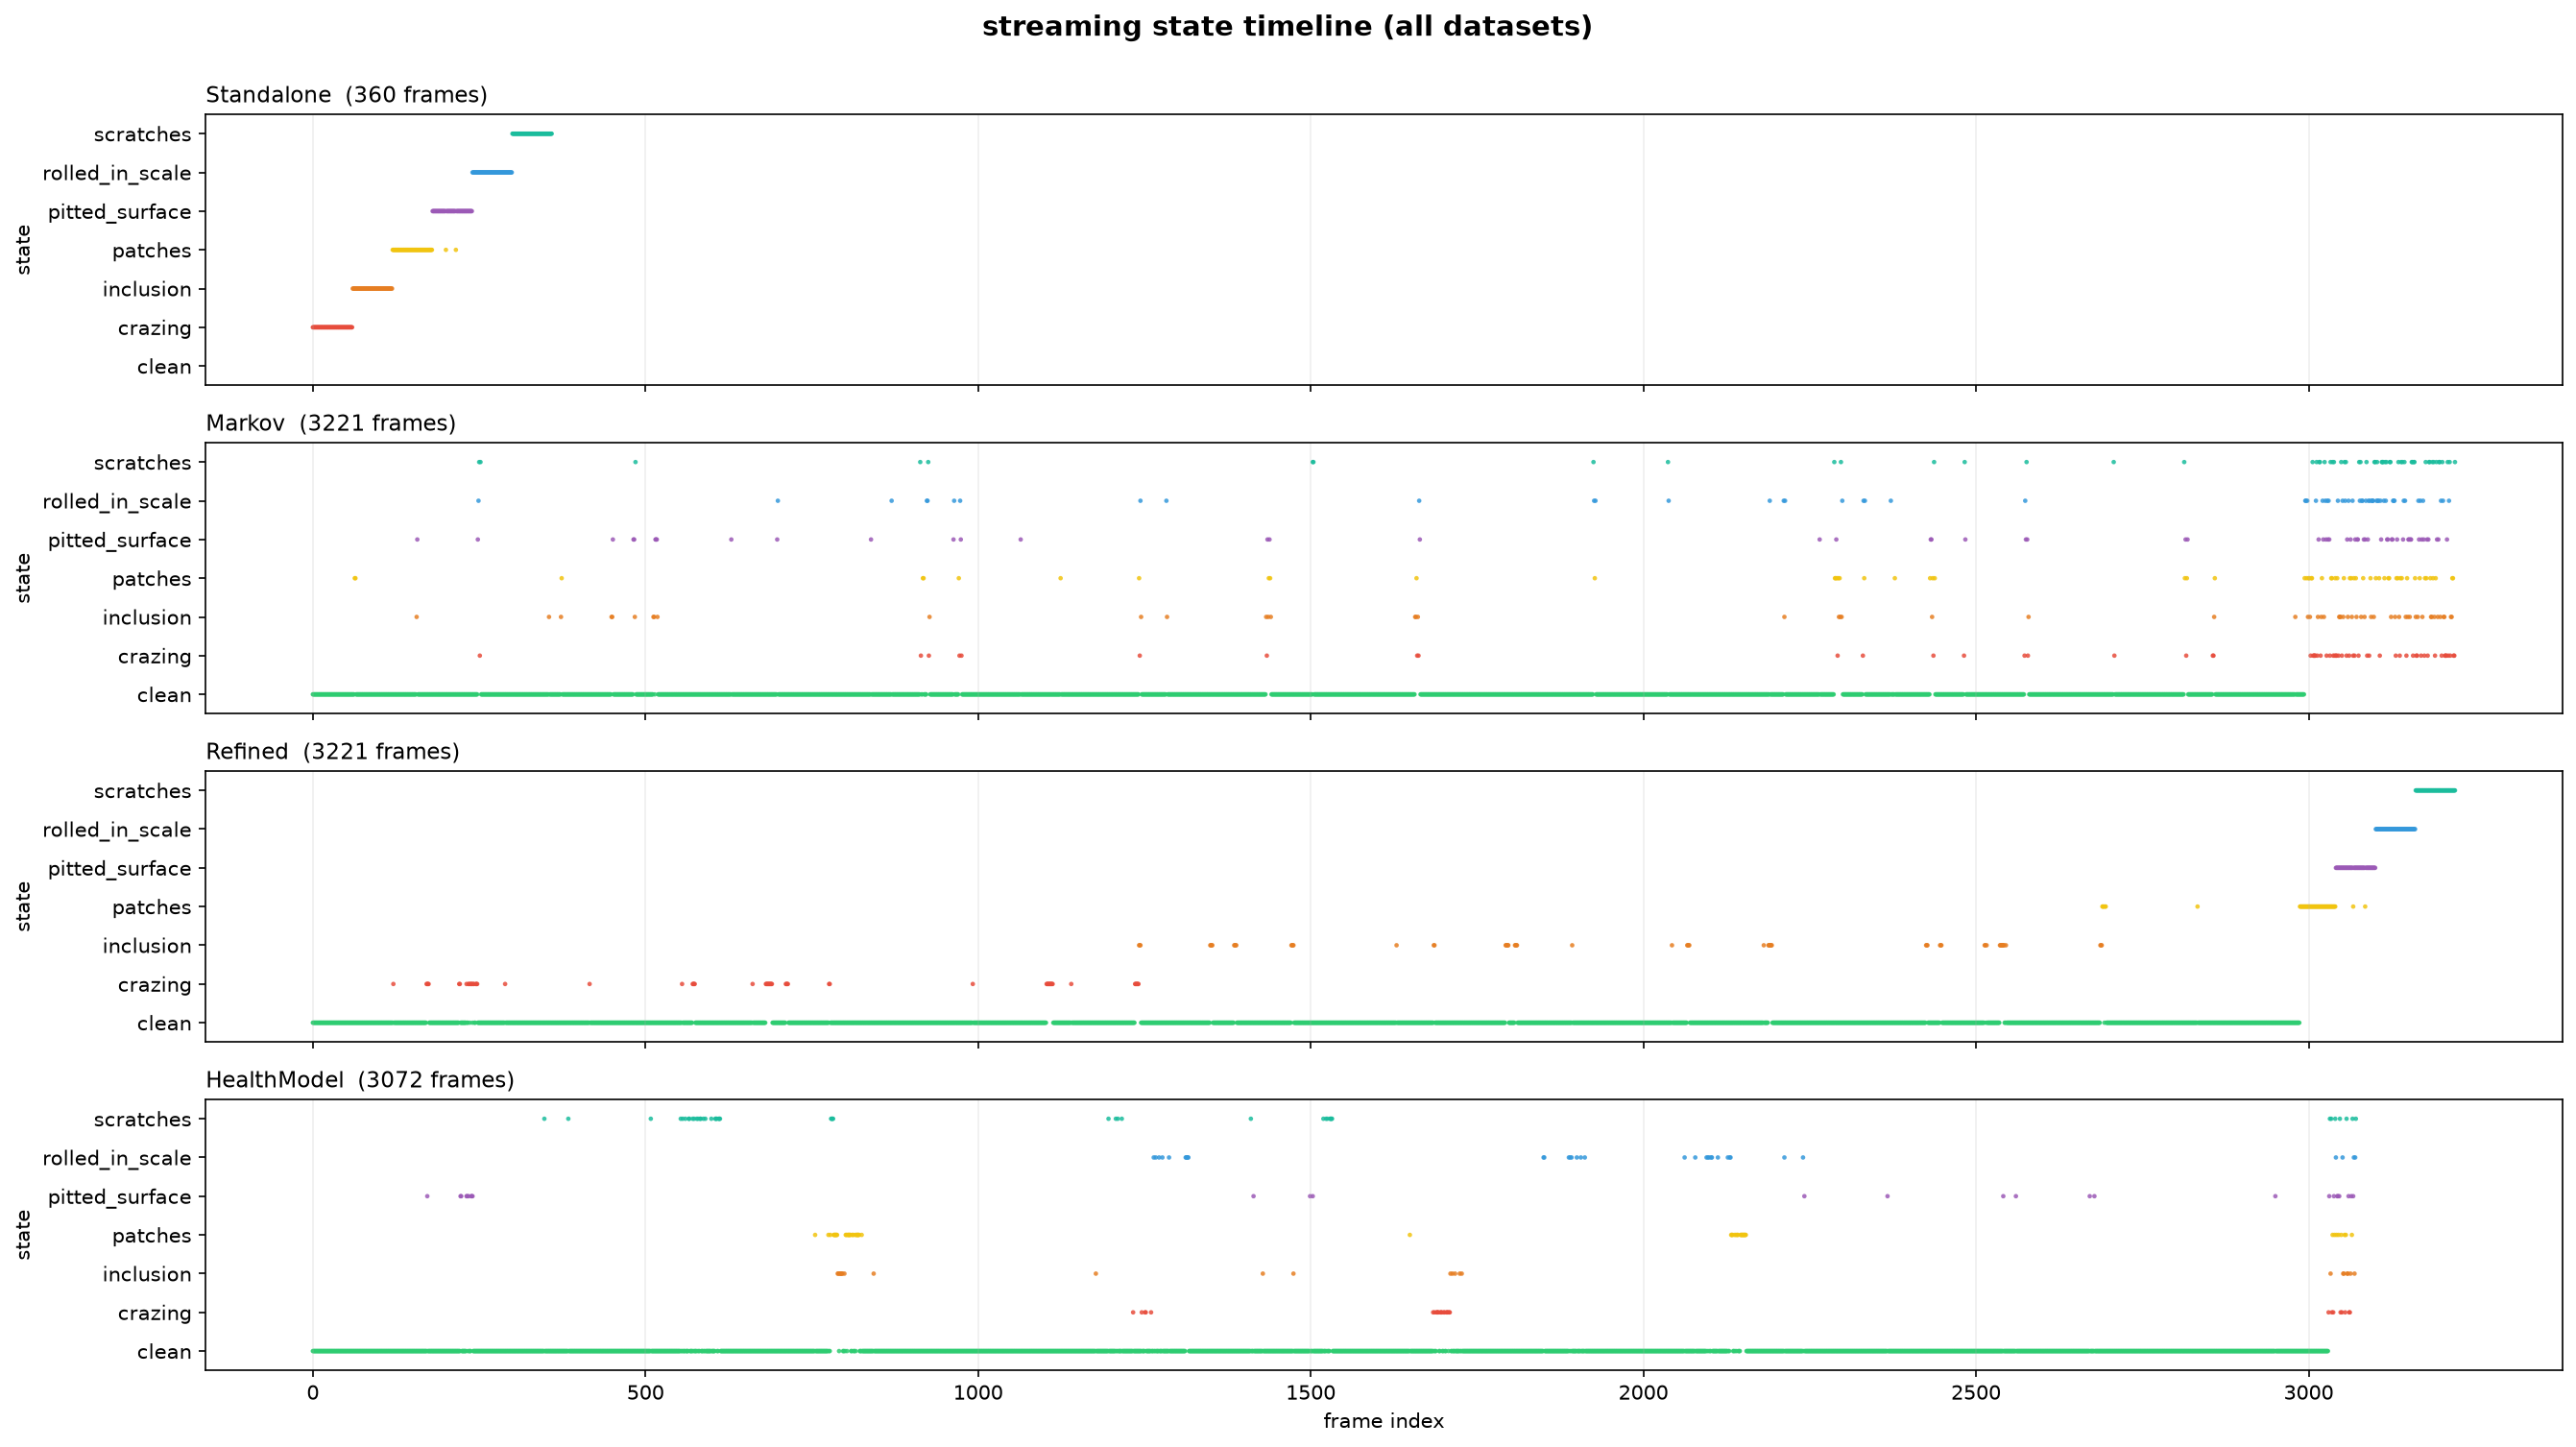
\includegraphics[width=0.8\linewidth, keepaspectratio]{img/timeline.png}
		\caption{نمودار سری زمانی}
		\label{fig:timeline}
	\end{figure}
	
	در شکل \ref{fig:transition} که ماتریس احتمالات انتقال حالات را مقایسه می‌کند، مدل \lr{Markov} دارای احتمالات یکنواخت و پراکنده ($0.10 - 0.25$) در تمام عناصر است که عدم وجود حافظه زمانی را اثبات می‌کند، مدل \lr{Refined} پایداری بسیار بالایی روی قطر اصلی ($0.67$ تا $0.98$) نشان می‌دهد که مانع از تغییر حالت ناگهانی می‌شود، و در نهایت مدل \lr{HealthModel} علاوه بر حفظ پایداری نسبی، احتمالات بازگشت منطقی به حالت پاک ($P(\mathrm{clean} \mid \mathrm{defect}) \approx 0.28 - 0.66$) را مدلسازی می‌کند.
	\begin{figure}[H]
		\centering
		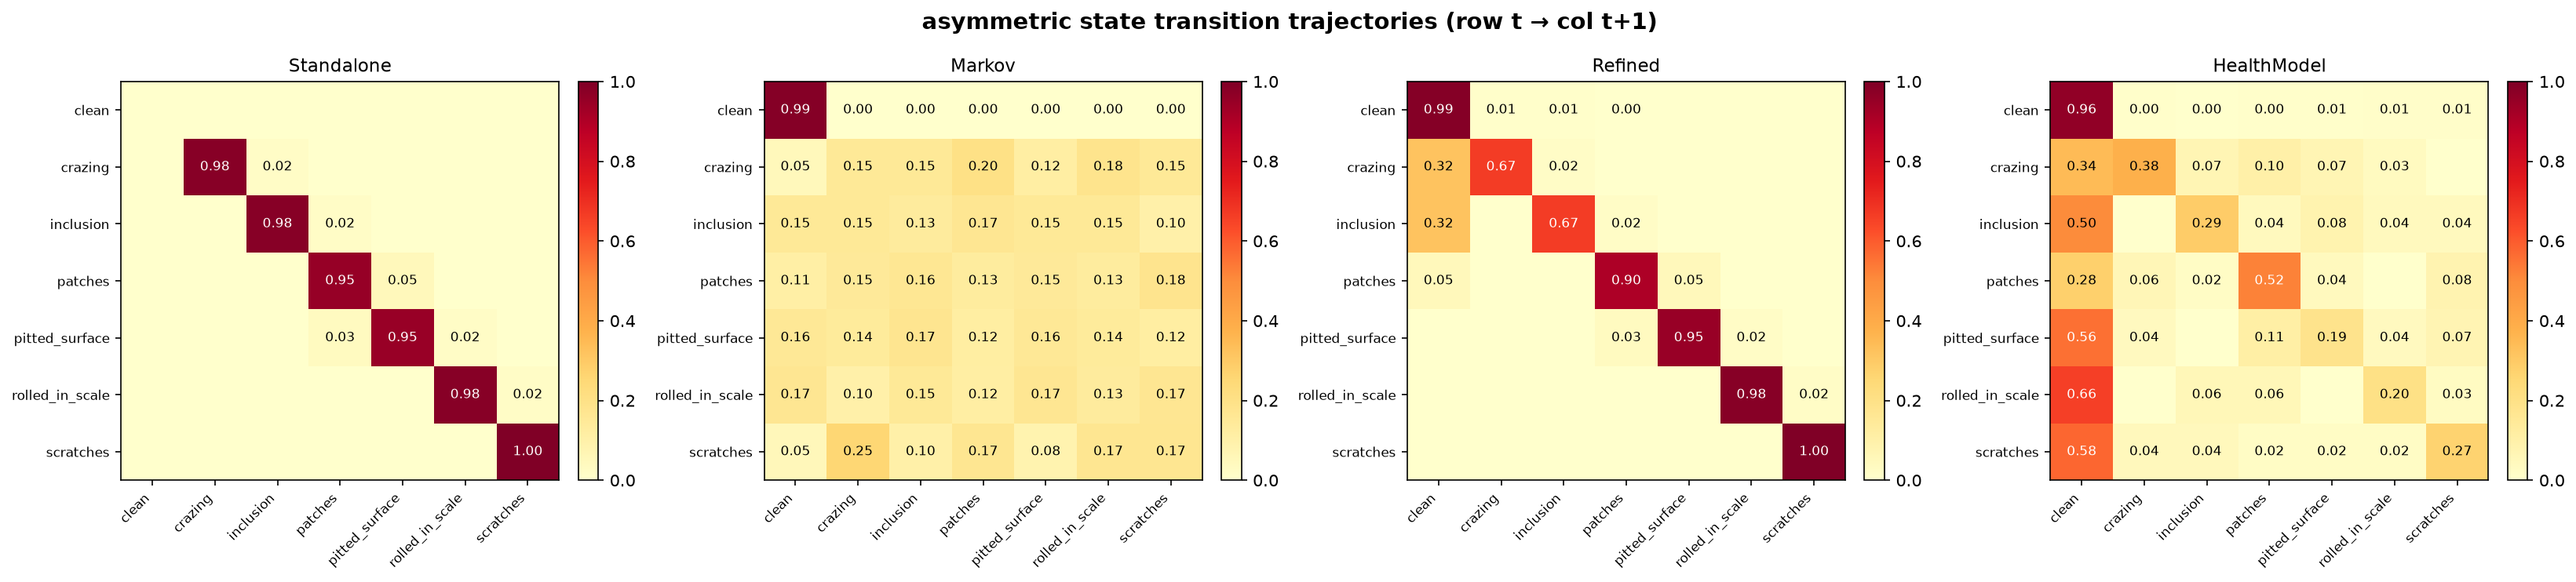
\includegraphics[width=0.8\linewidth, keepaspectratio]{img/transitionHeatMap.png}
		\caption{ماتریس احتمالات انتقال حالات}
		\label{fig:transition}
	\end{figure}
	
	
	\paragraph{نتیجه‌گیری} \mbox{} \\
	در مجموع و با مقایسه هر چهار بخش، مدل \lr{Health} مناسب‌ترین و واقع‌گرایانه‌ترین گزینه برای پایش پویای سلامت سیستم است، زیرا بر خلاف \lr{Markov} دچار نویز و پرش‌های لحظه‌ای نمی‌شود و بر خلاف \lr{Refined} که رفتار سخت‌گیرانه و قفل‌شده روی حالات دارد، قابلیت مدلسازی هموار، پیوسته و بازگشت‌پذیر عیوب را در طول زمان فراهم می‌سازد.
	\subsection{نمونه‌های شبیه‌سازی و چالش‌های عملیاتی مربوطه}
	\subsubsection*{نمونه اول: عدم تعادل شدید کلاس‌ها و جابه‌جایی توزیع عیوب نادر (\lr{Long-Tail / Rare Defect Shift})}
	
	در خطوط تولید پیوسته نورد گرم و سرد فولاد، توزیع عیوب سطحی به شدت ناهمگن بوده و از الگوی دنباله‌بلند (\lr{Long-Tail Distribution}) پیروی می‌کند. در عملیات واقعی، بخش اعظم سطوح تولیدی کاملاً سالم هستند یا حاوی عیوب متداول با فراوانی بالا مانند خراش و وصله می‌باشند؛ در حالی که عیوب بحرانی و ساختاری نظیر مقیاس نورد‌شده یا ناخالصی به ندرت رخ می‌دهند.
	
	اهمیت این چالش در سیستم‌های بینایی ماشین صنعتی از آنجا ناشی می‌شود که مدل‌های یادگیری عمیق متداول در صورت آموزش روی داده‌های متوازن، در مواجهه با جریان واقعی داده دچار سوگیری شدیدی به سمت کلاس‌های غالب شده و نرخ منفی کاذب (\lr{False Negative Rate}) عیوب نادر اما مهلک ساختاری افزایش می‌یابد. عدم شناسایی عیوبی مانند \lr{Inclusion} یا \lr{Rolled-in Scale} می‌تواند منجر به شکست ناگهانی قطعات فولادی زیر بار مکانیکی در صنایع حساس نظیر خودروسازی و سازه‌های عمرانی گردد.
	
	\paragraph{نحوه ساخت نمونه: }
	نمونه‌سازی به صورت یک جریان زمانی پیوسته از فریم‌های متوالی $t \in \{1, 2, \dots, N\}$ با مجموع $N = 3054$ فریم تنظیم شده است. الگوریتم نگاشت عیوب بر اساس تخصیص تصادفی اما کنترل‌شده نرخ وقوع عیوب با تابع توزیع احتمال چگال ناهمگون عمل می‌کند.
	
	برای هر فریم $t$، مجموعه جعبه‌های احاطه‌گر به صورت $B_t = \{(c_{i}, x_i, y_i, w_i, h_i)\}_{i=1}^{k_t}$ تعریف می‌شود که در آن $c_i \in C$ نشان‌دهنده شناسه کلاس، $(x_i, y_i)$ مرکز نرمال‌شده، و $(w_i, h_i)$ ابعاد نرمال‌شده جعبه در بازه $[0, 1]$ هستند. تعداد عیوب در هر فریم با $k_t \ge 0$ مشخص می‌گردد. مساحت کل درگیر عیوب در فریم $t$ بر اساس رابطه زیر محاسبه می‌شود:
	
	
	$$A_t = \sum_{i=1}^{k_t} w_{i,t} \cdot h_{i,t}$$
	
	توزیع کلاس‌ها تابع احتمال $P(c = c_j)$ را شبیه‌سازی می‌کند که در آن نرخ وقوع کلاس‌های نادر بسیار کوچکتر از کلاس‌های متداول است:
	
	
	$$P(c = \text{\lr{Inclusion}}) \ll P(c = \text{\lr{Scratches}})$$
	
	
	نمودارهای شکل \ref{fig:sample1} شامل دو محور موازی برای تحلیل جریان زمانی است.
	\begin{figure}[H]
		\centering
		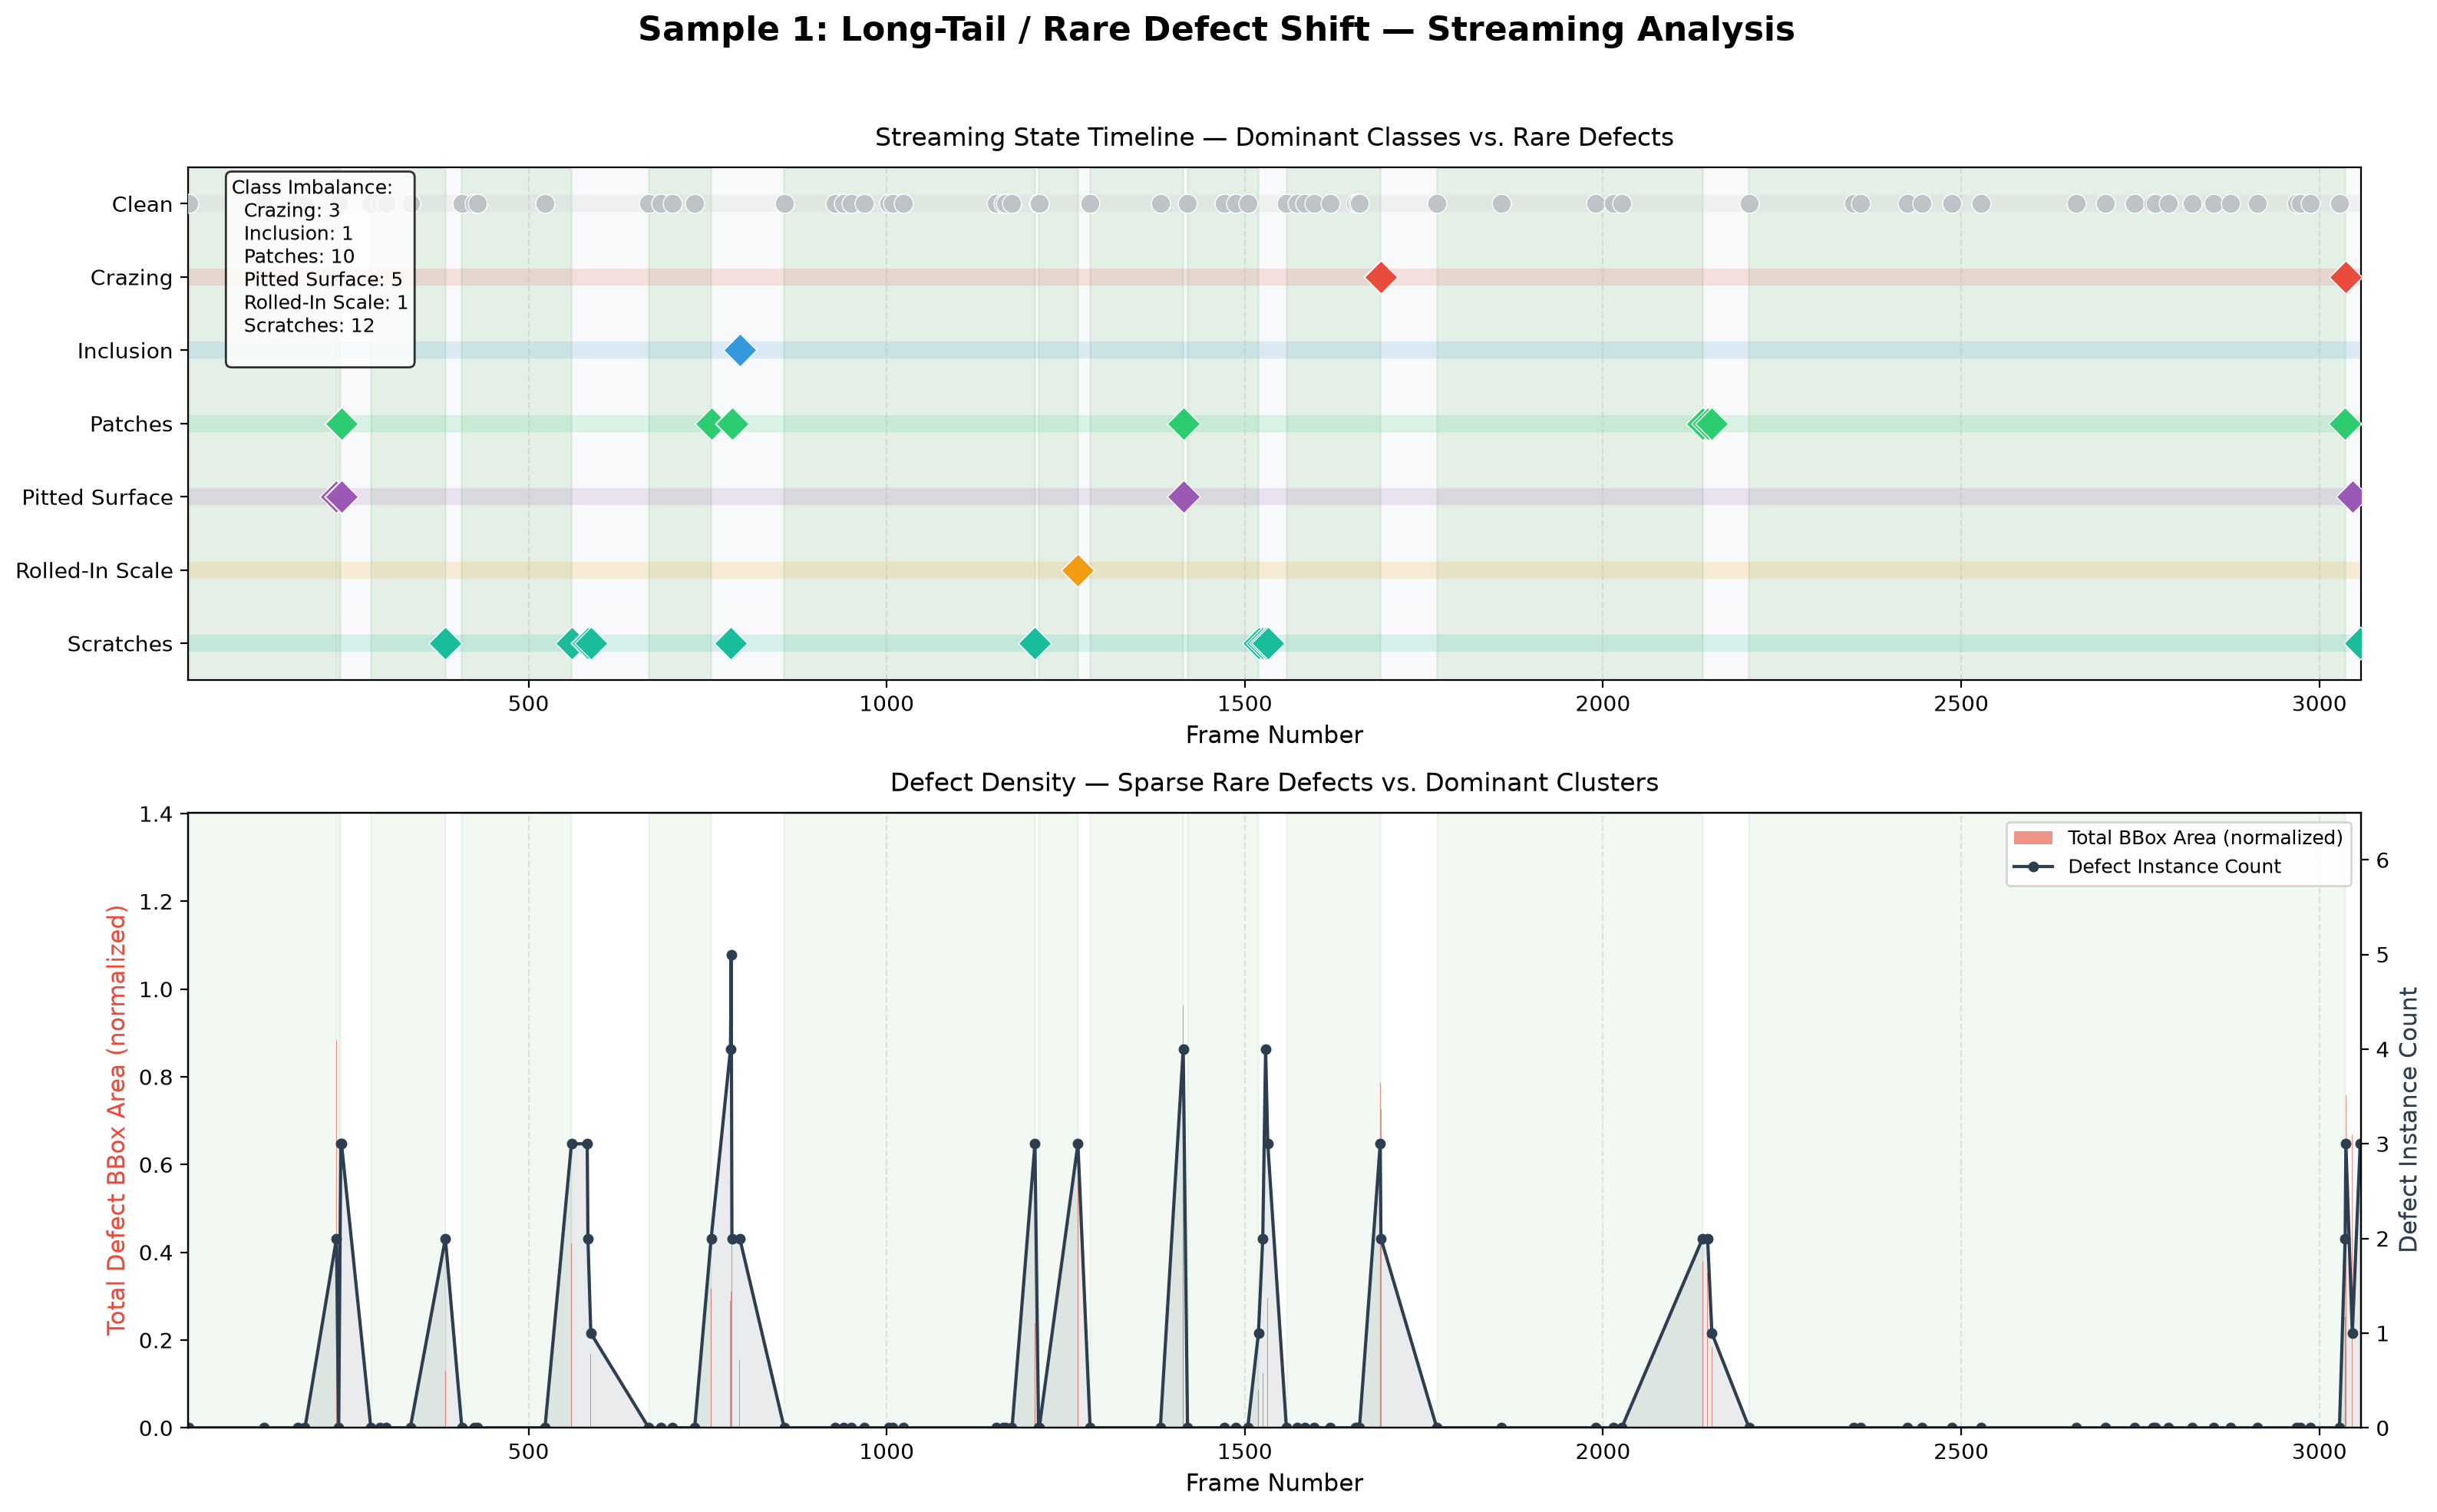
\includegraphics[width=0.8\linewidth, keepaspectratio]{img/sample1_visualization.png}
		\caption{تحلیل جریان زمانی نمونه اول}
		\label{fig:sample1}
	\end{figure}
	
	نمودار خط زمانی وضعیت جریان (\lr{Streaming State Timeline})، توزیع زمانی وقوع هر کلاس را نمایش می‌دهد. نواحی سبز‌رنگ عمودی نشان‌دهنده فریم‌های پاک و بدون عیب (\lr{Clean}) هستند که بخش اعظم محور زمان را پوشش داده‌اند. شکل‌های لوزی رنگی، زمان دقیق رخ‌داد عیوب مختلف را مشخص می‌کنند. نرخ عدم تعادل کلاس‌ها (\lr{Class Imbalance}) در جدول زیر خلاصه‌سازی شده است:
	
	\begin{table}[H]
		\centering
		\resizebox{\columnwidth}{!}{
		\begin{tabular}{cc}
			\toprule
			\textbf{تعداد فراوانی} & \textbf{نام کلاس عیب} \\
			\midrule
			$12$ & \lr{Scratches} \\
			$10$ & \lr{Patches} \\
			$5$ & \lr{Pitted Surface} \\
			$3$ & \lr{Crazing} \\
			$1$ & \lr{Inclusion} \\
			$1$ & \lr{Rolled-In Scale} \\
			\bottomrule
		\end{tabular}
	}
		\caption{توزیع فراوانی کلاس‌ها در نمونه اول}
		\label{tab:sample12}
	\end{table}
	
	
	نمودار چگالی عیوب (\lr{Defect Density})،  دارای دو محور عمودی است؛ محور چپ (میله‌های قرمز) مساحت نرمال‌شده کل جعبه‌های محیطی عیوب ($A_t$) را نشان می‌دهد و محور راست (خط تیره همراه با نقاط) تعداد رخ‌داد عیوب در هر فریم ($C_t = k_t$) را شبیه‌سازی می‌کند. همبستگی بالای بین مساحت و تعداد عیوب در خوشه‌های خاص (مانند حدود فریم $800$ و $1500$) نشان‌دهنده بروز طغیان‌های موضعی عیوب (\lr{Defect Bursts}) است، در حالی که فریم‌های نادر مانند فریم‌های حاوی \lr{Inclusion} یا \lr{Rolled-in Scale} به صورت نقاط منفرد و ایزوله در طول خط تولید ظاهر شده‌اند.
	
	
	\subsubsection*{نمونه دوم: منطقه عیوب با چگالی بالا (\lr{High-Density Defect Zone})}
	
	در خطوط نورد گرم فولاد، بروز اختلالات سخت‌افزاری یا ناپایداری‌های ترمومکانیکی—مانند فرسایش شدید یا شکستگی غلتک‌ها، نوسانات دما در کوره پیش‌گرم، و اختلال در سیستم پوسته‌زدایی آب داغ (\lr{Descaling System})—منجر به ایجاد مناطقی با چگالی بالای عیب می‌شود. در این سناریو، زنجیره‌ای از فریم‌های متوالی حاوی عیوب متعدد و پیچیده به تصویر کشیده می‌شوند.
	
	اهمیت این چالش در سیستم‌های هوشمند کنترل کیفیت در دو بعد تجلی می‌یابد: نخست، توانایی الگوریتم‌های شناساگر در تفکیک و مرزبندی چند عیب هم‌زمان (\lr{Multi-Defect Co-occurrence}) در یک ناحیه محدود، و دوم، ارزیابی توان محاسباتی و پایداری مدل در مواجهه با خطاهایی با مساحت و تعداد بالا. 
	
	عدم شناسایی به‌موقع این بحران‌ها می‌تواند منجر به آسیب سنگین به تجهیزات پایینی (\lr{Downstream Equipment})، پارگی ورق فولادی در حین نورد، و تولید انبوه محصولات ضایعاتی گردد.
	
	\paragraph{نحوه ساخت نمونه: }
	نمونه‌سازی دوم بر اساس فیلترسازی تفکیکی و انتخاب تعمدی فریم‌هایی با مساحت عیب بالا از مجموع داده‌های اولیه انجام شده است. مجموع کل فریم‌های نمونه‌برداری‌شده برابر با $N = 100$ است که بر اساس نسبت مشخص $R_d = 0.70$ (معادل $70\%$ فریم معیوب و $30\%$ فریم پاک) جداسازی شده‌اند.
	
	الگوریتم ابتدا تمام فریم‌ها را بر اساس مجموع مساحت نرمال‌شده جعبه‌های محیطی مرتب‌سازی نزولی می‌کند:
	
	
	$$\text{ScoredList} = \text{SortDescent}\left( \sum_{i=1}^{k_m} w_{i,m} \cdot h_{i,m} \right)$$
	
	سپس، تعداد $N_{\text{defect}} = \lfloor N \cdot R_d \rfloor = 70$ فریم با بالاترین چگالی مساحتی از بالای لیست انتخاب شده و با $N_{\text{clean}} = 30$ فریم سالم (که به صورت تصادفی انتخاب شده‌اند) ترکیب می‌شوند. در نهایت، فریم‌ها بر اساس شناسه زمانی اصلی خود مرتب می‌گردند تا توالی زمانی جریان حفظ شود.
	
	نمودار شکل \ref{fig:sample2}، رفتاری کاملاً متفاوت نسبت به نمونه اول نشان می‌دهد که نمادی از شرایط بحرانی خط تولید است:
	\begin{figure}[H]
		\centering
		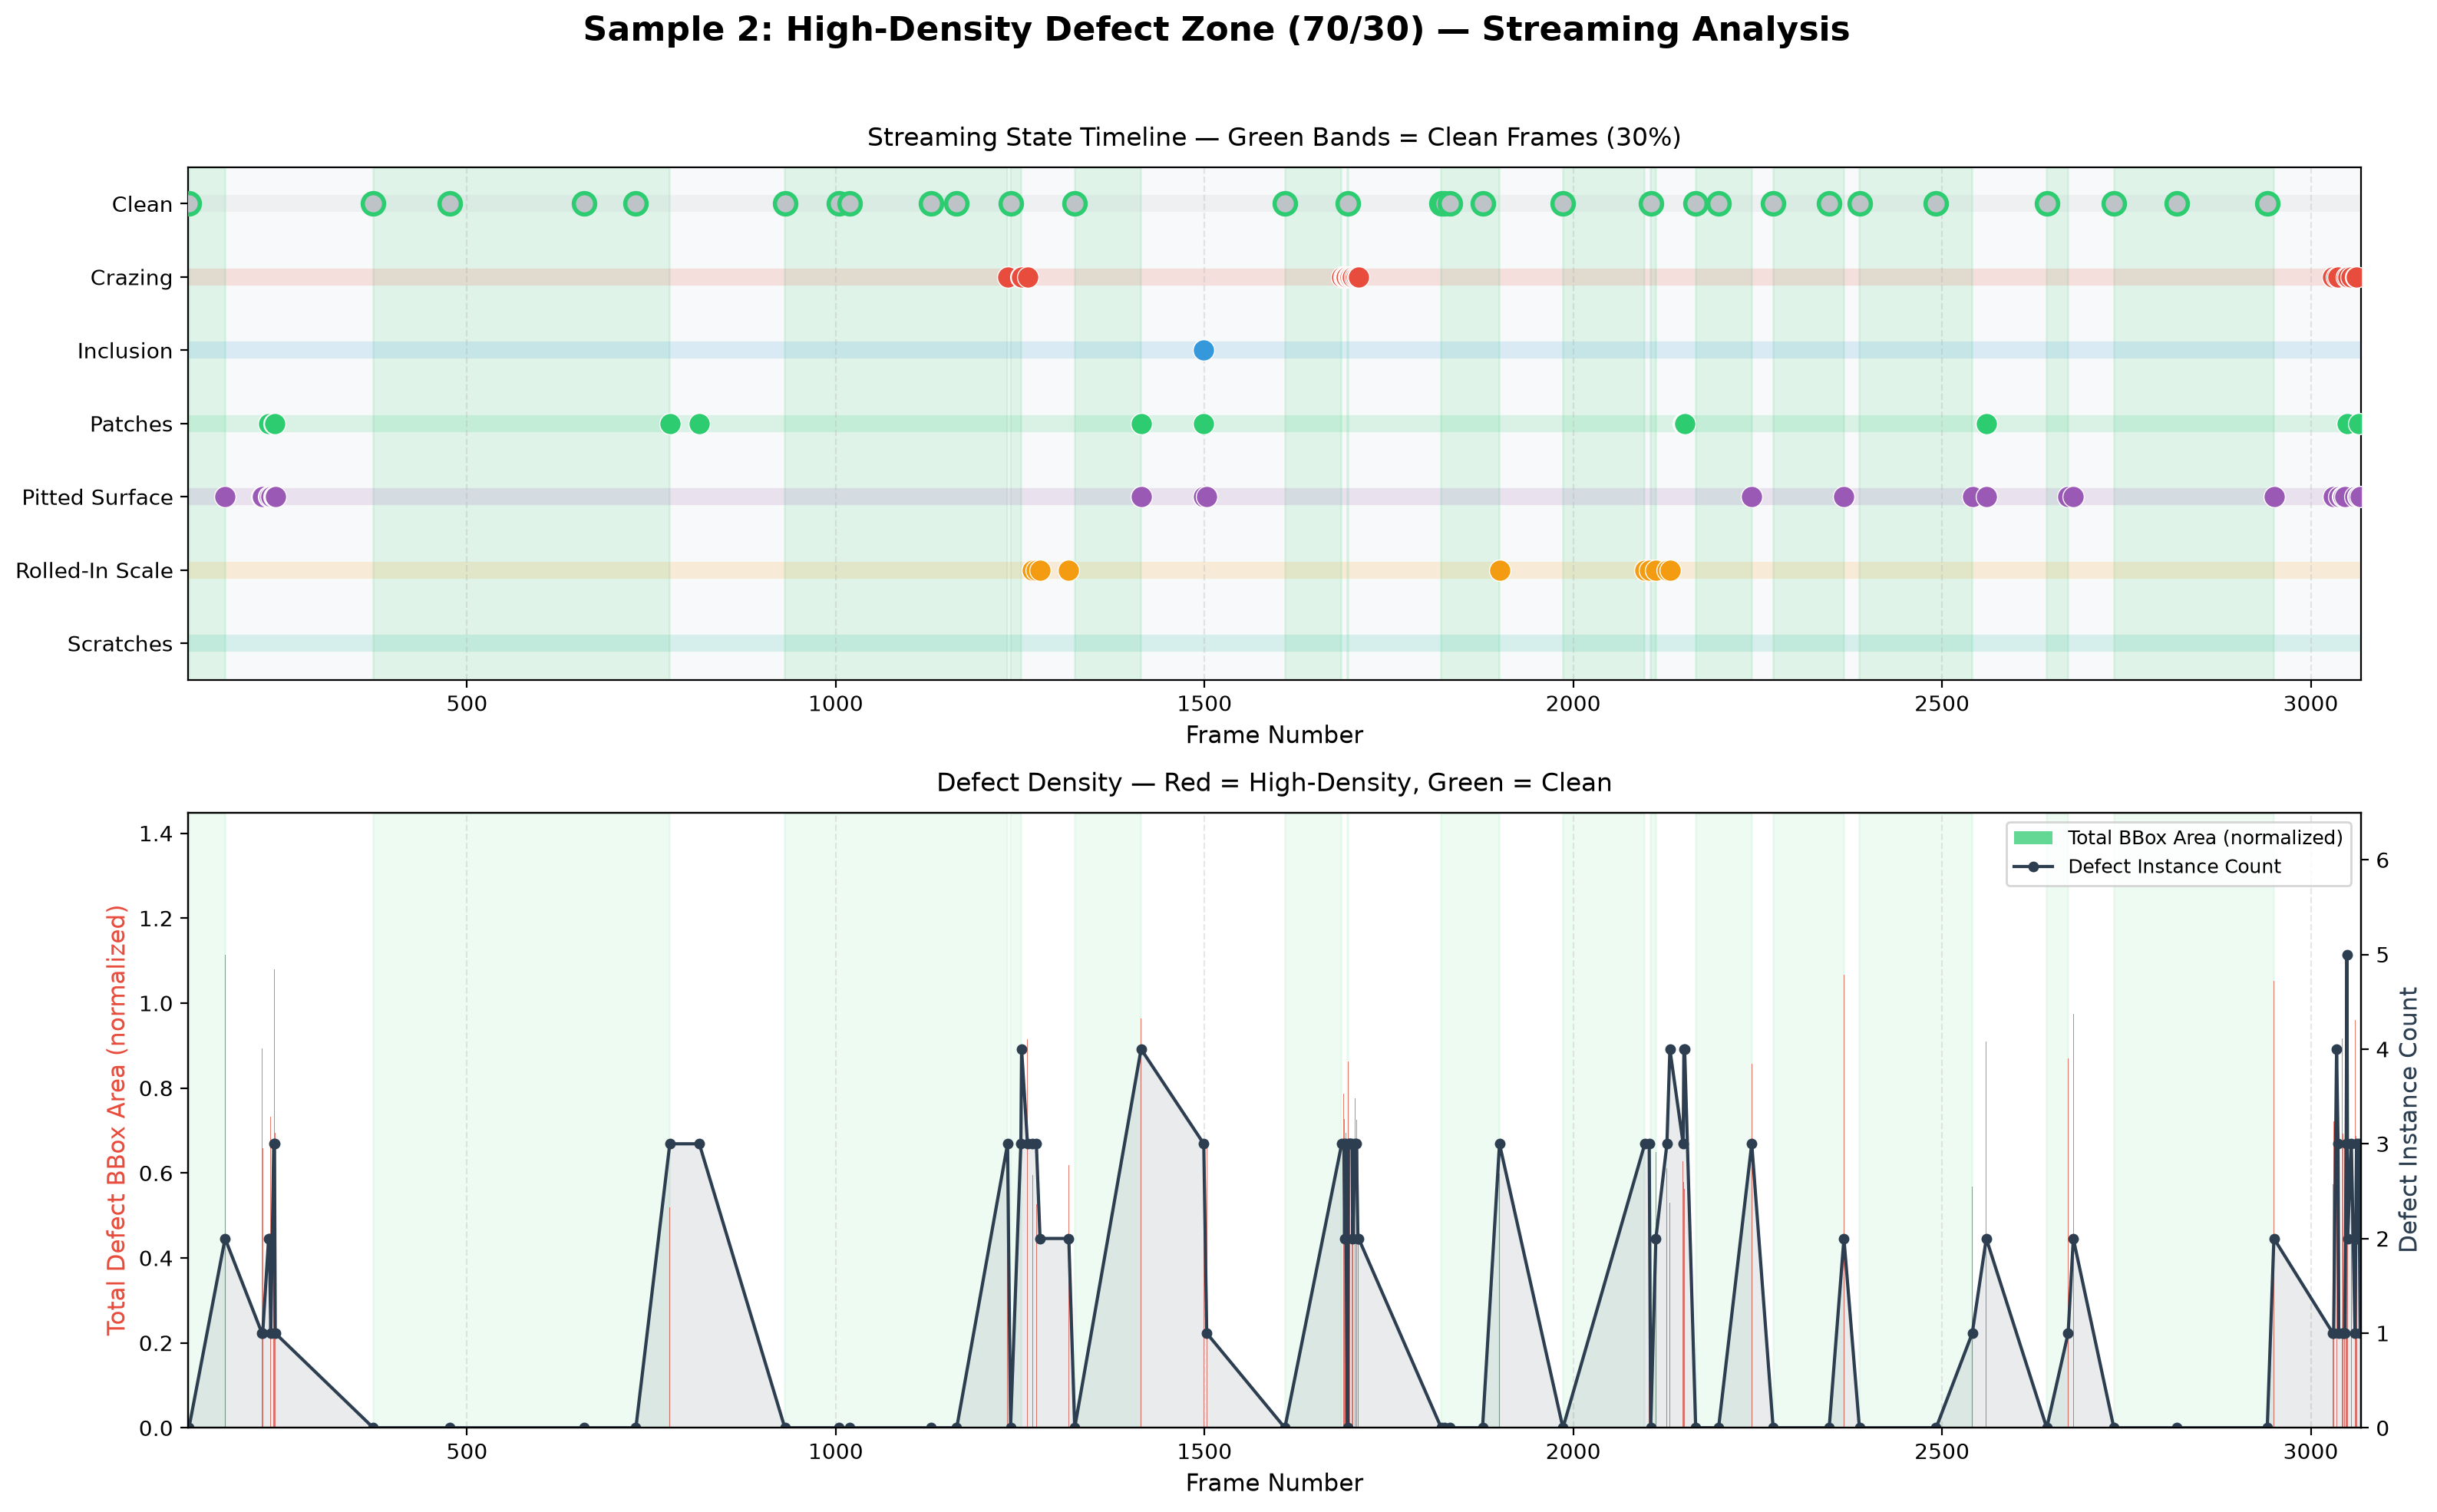
\includegraphics[width=0.8\linewidth, keepaspectratio]{img/sample2_high_density_viz.png}
		\caption{تحلیل جریان زمانی نمونه دوم}
		\label{fig:sample2}
	\end{figure}
	
	نمودار خط زمانی وضعیت جریان، بر خلاف نمونه اول، فریم‌های سالم که با نوارها و دایره‌های سبز رنگ مشخص شده‌اند، تنها $30\%$ از کل داده‌ها را تشکیل می‌دهند. حضور گسترده و فشرده کلاس‌های مختلف مانند \lr{Crazing}، \lr{Pitted Surface}، \lr{Patches} و \lr{Rolled-In Scale} در فریم‌های متوالی رخ داده است. 
	
	توزیع فراوانی کلاس‌های منحصر‌به‌فرد در این نمونه در جدول زیر آورده شده است:
	
	\begin{table}[H]
		\centering
		\resizebox{\columnwidth}{!}{
		\begin{tabular}{cc}
			\toprule
			\textbf{تعداد فراوانی} & \textbf{نام کلاس عیب} \\
			\midrule
			$30$ & \lr{Clean} \\
			$21$ & \lr{Pitted Surface} \\
			$10$ & \lr{Rolled-In Scale} \\
			$9$ & \lr{Crazing} \\
			$9$ & \lr{Patches} \\
			$1$ & \lr{Inclusion} \\
			$0$ & \lr{Scratches} \\
			\bottomrule
		\end{tabular}
	}
		\caption{توزیع فراوانی کلاس‌ها در نمونه دوم}
		\label{tab:sample1}
	\end{table}
	
	در نمودار چگالی عیوب ارتفاع میله‌های قرمز رنگ (مساحت کل جعبه‌های محیطی) و قله‌های خط تیره (تعداد عیوب در هر فریم) به طور چشمگیری افزایش یافته است. مقدار بیشینه تعداد عیوب در یک فریم به $5$ مورد و مساحت نرمال‌شده کل در برخی فریم‌ها به بیش از $1.0$ رسیده است. این تمرکز بالای عیوب، نشان‌دهنده وقوع رخ‌دادهای هم‌زمان چندین عیب در فریم‌های بحرانی است.
	
	\subsubsection*{نمونه سوم: جابه‌جایی آلیاژ و کنتراست (\lr{Alloy / Contrast Shift - Concept Drift})}
	
	در خطوط تولید انطباق‌پذیر فولاد، خط نورد برای تولید گریدها و آلیاژهای مختلف (مانند فولاد زنگ‌نزن، فولادهای پرکربن یا آلیاژهای دارای پوشش) تنظیم می‌شود. تغییر در ترکیب آلیاژی، ساختار کریستالی، و شرایط نورد گرم، منجر به تغییرات شدید در ویژگی‌های بصری سطح از جمله بازتابش نور، میزان تیرگی/روشنایی پایه، و کنتراست ظاهری بافت سطح می‌گردد.
	
	این پدیده در سیستم‌های یادگیری عمیق تحت عنوان رانش داده (\lr{Concept Drift / Covariate Shift}) شناخته می‌شود. هنگامی که یک مدل بینایی ماشین تنها روی یک گرید خاص از فولاد آموزش دیده باشد، تغییر مشخصات بصری تصویر پایه (حتی بدون تغییر در ماهیت هندسی عیوب) باعث می‌شود مدل در تشخیص لبه‌های عیوب دچار خطا شده و نرخ مثبت با منفی کاذب به شدت افزایش یابد.
	
	\paragraph{نحوه ساخت نمونه: }
	برای شبیه‌سازی جابه‌جایی آلیاژی، مجموعه ۱۰۰ فریمی شامل ۱۵ فریم معیوب (با پوشش حداقل یک نمونه از تمام کلاس‌های عیب) و ۸۵ فریم پاک انتخاب شده است. سپس روی تصاویر، تغییرات \lr{Photometric} اعمال شده است.
	
	تغییرات اعمال‌شده بر روی هر تصویر $I(x,y)$ به صورت متغیرهای تصادفی با توزیع یکنواخت $U(a, b)$ مدل‌سازی شده‌اند:
	\begin{itemize}
		\item \textbf{شدت روشنایی (\lr{Brightness}):} 
		$I_{\text{bright}} = \beta \cdot I$ که در آن $\beta \sim U(0.45, 0.70)$
		\item \textbf{کنتراست (\lr{Contrast}):} 
		$I_{\text{contrast}} = \gamma \cdot (I_{\text{bright}} - \bar{I}) + \bar{I}$ که در آن $\gamma \sim U(0.65, 1.35)$
		\item \textbf{اشباع رنگ و تیزنگاری (\lr{Color \& Sharpness}):}
		تغییرات تصادفی در بازه‌های $U(0.75, 1.05)$ و $U(0.85, 1.0)$
	\end{itemize}
	
	میانگین شدت روشنایی ($\mu$) و انحراف معیار کنتراست ($\sigma$) تصویر به صورت زیر محاسبه می‌شوند:
	
	
	$$\mu = \frac{1}{W \cdot H} \sum_{x=1}^{W} \sum_{y=1}^{H} I_{\text{gray}}(x,y)$$
	
	$$\sigma = \sqrt{\frac{1}{W \cdot H} \sum_{x=1}^{W} \sum_{y=1}^{H} (I_{\text{gray}}(x,y) - \mu)^2}$$
	
	
	نمودار شکل \ref{fig:sample3} تحلیل هم‌زمان جریان داده و تغییرات ویژگی‌های آماری تصویر را نمایش می‌دهد.
	\begin{figure}[H]
		\centering
		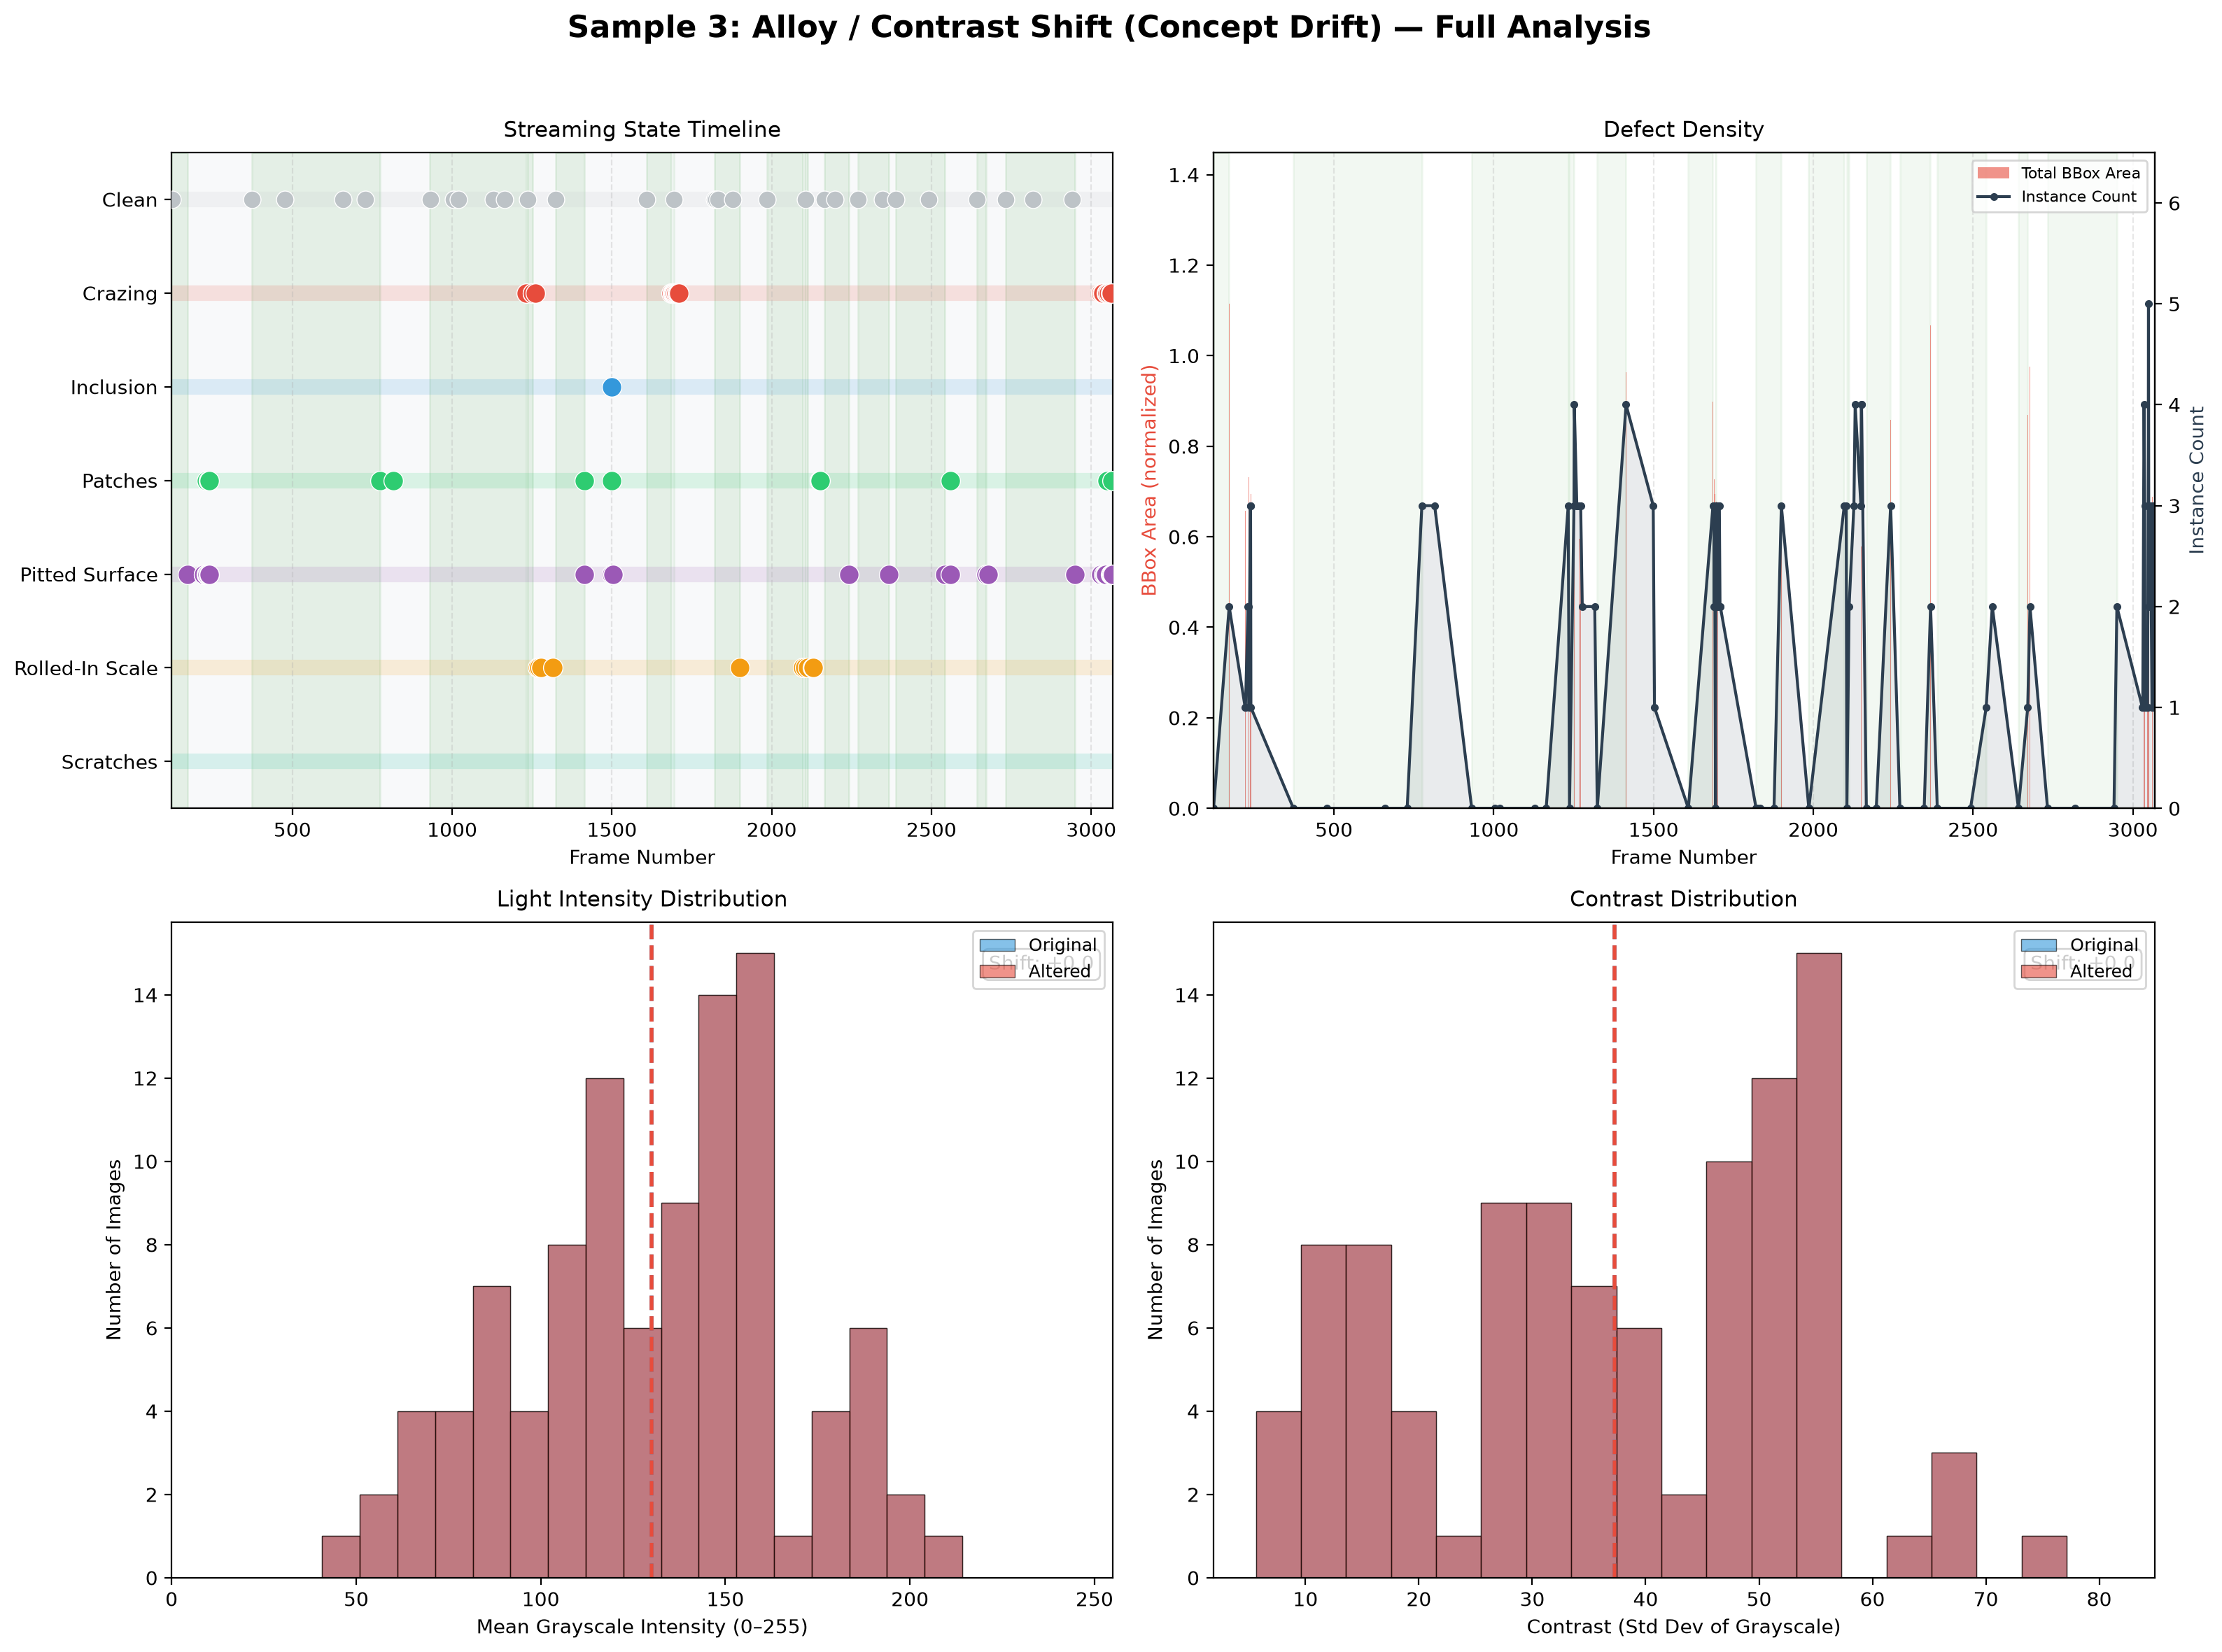
\includegraphics[width=0.8\linewidth, keepaspectratio]{img/sample3_shift_viz.png}
		\caption{تحلیل جریان زمانی و تغییرات ویژگی‌های آماری نمونه سوم}
		\label{fig:sample3}
	\end{figure}
	
	نمودار خط زمانی وضعیت جریان و چگالی عیوب نشان می‌دهد توزیع ۱۵ فریم معیوب در کنار فریم‌های پاک شبیه‌سازی شده است. تمرکز عیوب متداول و نادر در طول محور زمان حفظ شده است. 
	
	جدول توزیع کلاس‌ها به شرح زیر است:
	
	\begin{table}[H]
		\centering
		\resizebox{\columnwidth}{!}{
		\begin{tabular}{cc}
			\toprule
			\textbf{تعداد فراوانی} & \textbf{نام کلاس عیب} \\
			\midrule
			$85$ & \lr{Clean} \\
			$4$ & \lr{Patches} \\
			$4$ & \lr{Pitted Surface} \\
			$3$ & \lr{Crazing} \\
			$3$ & \lr{Rolled-In Scale} \\
			$1$ & \lr{Inclusion} \\
			$0$ & \lr{Scratches} \\
			\bottomrule
		\end{tabular}
	}
		\caption{توزیع فراوانی کلاس‌ها در نمونه سوم}
		\label{tab:sample3}
	\end{table}
	
	
	نمودار توزیع شدت نور (\lr{Light Intensity Distribution})، توزیع میانگین مقادیر خاکستری فریم‌ها را نشان می‌دهد. خط چین قرمز رنگ میانگین کل مجموعه ($\text{\lr{tShift}} \approx 130$) را نشان می‌دهد. افت روشنایی بین $45\%$ تا $70\%$ سبب انتقال جابه‌جایی دامنه روشنایی به سمت مقادیر پایین‌تر (تصاویر تیره‌تر) شده است.
	
	نمودار توزیع کنتراست (\lr{Contrast Distribution})،  توزیع انحراف معیار مقادیر خاکستری را نمایش می‌دهد که میانگین آن در حدود $\text{\lr{tShift}} \approx 37.3$ قرار گرفته است. پراکندگی بالای این نمودار شبیه‌ساز دقیق تغییرات بافت و بازتابش نور در اثر تغییر آلیاژ ورق فولادی در خط تولید واقعی است.
	
	\subsection{پیشنهادها و بهبودهای آتی برای مجموعه داده (آموزش و اعتبارسنجی)}
	
	ارزیابی‌های انجام‌شده بر روی مجموعه داده اصلی \lr{NEU-DET} و تحلیل هندسی/آماری عیوب نشان می‌دهد که اگرچه این بنچمارک پایهٔ مناسبی برای آموزش و اعتبارسنجی مدل‌های بینایی ماشین در محیط \lr{Webots} فراهم می‌آورد، اما برای رسیدن به سطح عملیاتی قابل اتکا در خطوط واقعی تولید، نیازمند اصلاحات و بهبودهای ساختاری در دو فاز آموزش (\lr{Train}) و اعتبارسنجی (\lr{Validation}) است.
	
	\subsubsection*{بهبودهای پیشنهادی برای مجموعه داده آموزش}
	
	\paragraph{استخراج و تزریق نمونه‌های منفی سخت (\lr{Hard Negative Mining}): }
	
	یکی از مهم‌ترین چالش‌های مدل‌های آشکارساز در خط تولید، نرخ بالای آلارم کاذب (\lr{FPR}) در مواجهه با پس‌زمینه‌های سالم پیچیده است. در روش \lr{Hard Negative Mining}، نمونه‌هایی از پس‌زمینه اعتبارسنجی که دارای بافت مشابه عیوب هستند (اما فاقد عیب واقعی‌اند) شناسایی و به مجموعه آموزش اضافه می‌گردند. این فرایند به مدل کمک می‌کند تا تفاوت‌های ظریف میان بافت سالم و عیب‌های واقعی را با دقت بیشتری فرا گیرد و در نتیجه چشمگیر \lr{FPR} در خط تولید واقعی کاهش یابد.
	
	\paragraph{داده‌افزایی مبتنی بر مدل مولد و آگاه از فیزیک (\lr{Generative and Physics-Aware Augmentation}): }
	
	با توجه به کمیابی برخی کلاس‌های عیب (به‌ویژه \lr{Inclusion}) در مجموعه داده اصلی، استفاده از مدل‌های مولد مانند \lr{Diffusion Models} یا شبکه‌های متخاصم (\lr{GANs}) برای تولید ستون‌های عیب نادر پیشنهاد می‌شود. این روش علاوه بر افزایش تنوع هندسی، قابلیت تنظیم پارامترهای فیزیکی مانند تاری حرکتی (\lr{Motion Blur}) و تغییرات روشنایی متناظر با خط نورد را دارد. به‌عنوان مثال، می‌توان عیوب \lr{Inclusion} را با کنتراست‌های متفاوت و در پس‌زمینه‌های بافتی گوناگون تولید کرد تا مدل در برابر تغییرات محیطی پایدارتر گردد.
	
	\paragraph{متوازن‌سازی توزیع کلاس‌ها و ابعاد (\lr{Class and Scale Re-balancing}): }
	
	توزیع نابرابر کلاس‌ها در \lr{NEU-DET} (هر چند از نظر تعداد برابر است، اما از نظر تنوع هندسی و مقیاس غیریکنواخت است) می‌تواند منجر به سوگیری مدل به سمت عیوب بزرگ‌تر و پرتکرارتر شود. با اعمال  \lr{Re-balancing}، نمونه‌های عیوب کوچک و کلاس‌های نادر در دسته‌بندی اولیه وزن‌دهی شده و در داده‌های آموزش به‌صورت متوازن‌تری توزیع می‌گردند.
	
	\subsubsection*{بهبودهای پیشنهادی برای مجموعه داده اعتبارسنجی}
	
	\paragraph{داده‌های زمانی پیوسته (\lr{Continuous Temporal Data}): }
	
	مجموعه داده اعتبارسنجی اصلی \lr{NEU-DET} به‌صورت تصاویر ایستا (\lr{Static Images}) است. در حالی که در خط تولید واقعی، ورق فولاد به‌صورت پیوسته از مقابل دوربین عبور می‌کند. با استفاده از الگوریتم \lr{Image Stitching}، می‌توان فریم‌های مجزا را به توالی‌های ویدئویی با نرخ فریم (\lr{FPS}) واقعی تبدیل کرد. این امر امکان سنجش پایداری زمانی (\lr{Temporal Consistency}) مدل را فراهم می‌آورد؛ به‌طوری‌که مدل نباید در فریم‌های متوالی و مشابه، خروجی‌های متناقض (\lr{Flickering}) تولید کند.
	
	\subsubsection*{ارتقا از \lr{Bounding Box} به \lr{Segmentation}}
	
	برای عیوبی که مرزهای نامنظم و پیچیده دارند (مانند \lr{Crazing} و \lr{Patches})، مستطیل‌های محدودکننده (\lr{Bounding Boxes}) حاوی مقادیر زیادی پس‌زمینه سالم هستند که ارزیابی دقت \lr{IoU} را مخدوش می‌کند. پیشنهاد می‌شود برچسب‌های اعتبارسنجی به ماسک‌های چندضلعی (\lr{Polygonal Masks}) ارتقا یابند. این روش با تفکیک دقیق‌تر پیکسل‌های عیب از پس‌زمینه، امکان محاسبهٔ دقیق‌تر شاخص \lr{IoU} و ارزیابی کیفی بهتر را فراهم می‌سازد.
	
	
	% -----------------------------------------------------
	\subsection{ پیاده‌سازی بازوی رباتیک نشانه‌گذار در خط تولید فولاد}
	
	\subsubsection*{بررسی نیازمندی‌های صنعتی}
	در فرآیندهای مدرن نورد و تولید ورق‌های فولادی، شناسایی و نشانه‌گذاری آنی عیوب سطحی از اهمیت بالایی برخوردار است. خطوط تولید فولاد به‌صورت مداوم در حال حرکت هستند و سرعت خط بر اساس تصمیمات سیستم‌های کنترلی به‌صورت دینامیک بین $0.1 \text{ m/s}$ تا $0.4 \text{ m/s}$ تغییر می‌کند. در چنین محیطی، بازوی رباتیک نشانه‌گذار باید دارای ویژگی‌های زیر باشد:
	\begin{itemize}
		\item \textbf{سرعت پاسخ‌دهی بالا (\lr{Real-time Response}):} فاصله زمانی بین تشخیص عیب توسط دوربین بازرسی تا رسیدن ورق به محور نشانه‌گذاری بسیار کوتاه است. بنابراین، الگوریتم کنترلی باید نرخ محاسبه و اعمال فرمان حرکتی را در گام‌های زمانی $32 \text{ ms}$ تنظیم کند.
		\item \textbf{دقت نشانه‌گذاری غیرکنتاکتی (\lr{Non-contact Marking Accuracy}):} به‌منظور جلوگیری از آسیب فیزیکی به نازل نشانه‌گذار یا ایجاد خط و خش روی ورق گرم، عمل نشانه‌گذاری با استفاده از مدولاسیون ابزار غیرکنتاکتی (مانند پاشش جوهر یا لیزر) انجام می‌شود که در محیط شبیه‌سازی با گره \lr{Pen} مدل‌سازی شده است.
		\item \textbf{پایداری دینامیکی (\lr{Dynamic Stability}):} با توجه به متغیر بودن سرعت نوار نقاله، موقعیت هدف و سرعت خطی/زاویه‌ای بازو باید به‌گونه‌ای محاسبه شود که از اورشوت (\lr{Overshoot}) و نوسانات مکانیکی جلوگیره شده و عمل پاشش دقیقاً در مرکز هندسی عیب انجام گیرد.
	\end{itemize}
	
	محیط شبیه‌سازی \lr{Webots} امکان شبیه‌سازی دقیق فیزیک اجسام صلب، دینامیک مفصل، گرانش، و اصطکاک را در یک محیط سه بعدی فراهم می‌سازد.
	
	\subsubsection*{معماری سیستم، مدل‌سازی ریاضی و الگوریتم‌های کنترل}
	
	\paragraph{فرمول‌بندی سینماتیک و دینامیک مفصل دورانی (\lr{Revolute Joint}): } \mbox{} \\
	اگرچه حرکت عرضی نشانه‌گذار را می‌توان با مفصل کشویی (\lr{LinearJoint}) پیاده‌سازی کرد، اما مدل‌سازی آن با مفصل دورانی (\lr{Revolute Joint}) نیازمند تبدیل موقعیت خطی استخراج‌شده از تصویر به زاویه چرخش مفصل است. اگر فرض کنیم بازویی به طول $L$ حول محور $Z$ می‌چرخد تا نازل نشانه‌گذار را در موقعیت عرضی $y_{\text{target}}$ قرار دهد:
	
	معادله سینماتیک مستقیم موقعیت عرضی نازل
	
	
	$$y_{\text{arm}} = L \cdot \sin(\theta)$$
	
	است و معادله سینماتیک معکوس برای محاسبه زاویه هدف مفصل ($\theta_{\text{target}}$) به صورت
	
	
	$$\theta_{\text{target}} = \arcsin\left(\frac{y_{\text{target}}}{L}\right)$$
	
	نوشته می‌شود.
	
	همچنین رابطه سرعت خطی عرضی ($v_y$) با سرعت زاویه‌ای مفصل ($\dot{\theta}$) به صورت زیر است:
	
	$$v_y = L \cdot \cos(\theta) \cdot \dot{\theta} \implies \dot{\theta} = \frac{v_y}{L \cdot \cos(\theta)}$$
	
	در نتیجه، دینامیک مفصل دورانی با در نظر گرفتن ممان اینرسی $J$، ضریب اصطکاک ویسکوز $B$ و گشتاور اعمالی موتور $\tau_m$ به‌صورت زیر فرمول‌بندی می‌شود:
	
	$$J \ddot{\theta} + B \dot{\theta} + \tau_g(\theta) = \tau_m$$
	
	که در آن $\tau_g(\theta)$ گشتاور ناشی از گرانش است. در الگوریتم پیاده‌سازی شده، نگاشت خطی مستقیم روی متغیر حالت عرضی انجام پذیرفته است.
	
	\subsection*{ساختار الگوریتم کنترل موقعیت/سرعت (کنترل‌کننده \lr{PID} و پروفیل برنامه‌ریزی مسیر)}
	سرعت واقعی نوار نقاله بر حسب متر بر ثانیه ($v_{\text{conveyor}}$) از روی سرعت تنظیم‌شده سیستم ($S$) و ضریب مقیاس فیزیکی ($\alpha = 0.03$) در هر گام زمانی ($\Delta t = 0.032 \text{ s}$) محاسبه می‌شود:
	
	
	$$v_{\text{conveyor}} = \frac{S \cdot \alpha}{\Delta t}$$
	
	زمان باقی‌مانده تا رسیدن عیب به خط محور نشانه‌گذار ($t_{\text{reach}}$) با توجه به فاصله طولی دوربین تا ابزار نشانه‌گذار ($X_{\text{offset}} = 0.3 \text{ m}$) و انحراف طولی عیب در تصویر ($\Delta x$) برابر است با:
	
	
	$$t_{\text{reach}} = \frac{X_{\text{offset}} - \Delta x}{v_{\text{conveyor}}}$$
	
	سرعت عرضی مورد نیاز برای جابه‌جایی بازو از موقعیت فعلی ($y_{\text{current}}$) به موقعیت هدف ($y_{\text{target}}$) به‌صورت زیر برنامه‌ریزی می‌شود:
	
	
	$$v_y = \frac{y_{\text{target}} - y_{\text{current}}}{\max(t_{\text{reach}}, 0.001)}$$
	
	این سرعت محاسبه‌شده مستقیم به عنوان ورودی به موتور اعمال می‌شود (\lr{\texttt{marker\_motor.setVelocity(abs(v\_y))}}) و موقعیت هدف نیز تنظیم می‌گردد (\lr{\texttt{marker\_motor.setPosition(y\_target)}}) تا حلقه‌ی کنترلی \lr{PID} داخلی \lr{Webots} خطای موقعیت را صفر کند.
	
	\paragraph{الگوریتم نگاشت مختصات عیوب تصویری به زاویه مفصل ربات} \mbox{}
	ابعاد تصویر ورودی $256 \times 256$ پیکسل است. ارتفاع دوربین $Z_{\text{camera}} = 0.96 \text{ m}$ و ارتفاع سطح ورق فولادی $Z_{\text{plate}} = 0.520 \text{ m}$ می‌باشد. فاصله عمودی برابر است با:
	
	$$\Delta Z = Z_{\text{camera}} - Z_{\text{plate}} = 0.44 \text{ m}$$
	
	با توجه به میدان دید دوربین (\lr{FOV})، فاکتور تبدیل پیکسل به متر (\lr{\texttt{METERS\_PER\_PIXEL}}) به‌صورت زیر استخراج شده است:
	
	
\begin{equation*}
	\resizebox{\columnwidth}{!}{%
		$\displaystyle
		\text{METERS\_PER\_PIXEL} = \frac{2 \cdot \Delta Z \cdot \tan(22.5^\circ)}{W_{\text{img}}} = \frac{2 \cdot 0.44 \cdot 0.41421356}{256} \approx 0.001424 \text{ m/pixel}
		$%
	}
\end{equation*}
	
	اگر مرکز باکس شناسایی‌شده عیب در تصویر برابر با $(u, v)$ باشد، انحراف فیزیکی نسبت به مرکز تصویر به‌صورت زیر محاسبه می‌شود:
	
	
	$$\Delta x = \left(u - \frac{W_{\text{img}}}{2}\right) \cdot \text{METERS\_PER\_PIXEL}$$
	
	$$\Delta y = \left(v - \frac{H_{\text{img}}}{2}\right) \cdot \text{METERS\_PER\_PIXEL}$$
	
	موقعیت جهانی عیب در راستای عرضی ($y_{\text{defect\_world}}$) و موقعیت هدف مفصل ربات ($y_{\text{target}}$) به‌دست می‌آید:
	
	
	$$y_{\text{defect\_world}} = Y_{\text{camera}} + \Delta y$$
	
	$$y_{\text{target}} = y_{\text{defect\_world}} - Y_{\text{pen\_base}}$$
	
	در نهایت پارامترهای هندسی سیستم در محیط شبیه‌سازی در جدول \ref{tab:par} قابل مشاهده هستند.
	\begin{table}[H]
		\centering
		\resizebox{\columnwidth}{!}{
		\begin{tabular}{ccc}
			\toprule
			\textbf{نماد ریاضی / متغیر} & \textbf{مقدار / واحد} & \textbf{توصیف پارامتر} \\
			\midrule
			$\Delta t$ & $32 \text{ ms}$ & گام زمانی شبیه‌سازی (\lr{TIME\_STEP}) \\
			$Z_{\text{camera}}$ & $0.96 \text{ m}$ & ارتفاع نصب دوربین بازرسی \\
			$Z_{\text{plate}}$ & $0.520 \text{ m}$ & ارتفاع سطح ورق فولادی \\
			$W_{\text{img}} \times H_{\text{img}}$ & $256 \times 256$ & رزولوشن تصویر دوربین \\
			$\text{METERS\_PER\_PIXEL}$ & $\approx 0.001424 \text{ m}$ & مقیاس تبدیل پیکسل به متر \\
			$X_{\text{offset}}$ & $0.3 \text{ m}$ & فاصله طولی مرکز دوربین تا نازل نشانه‌گذار \\
			\bottomrule
		\end{tabular}
	}
		\caption{پارامترهای هندسی و سیستم نشانه‌گذار در محیط شبیه‌سازی}
		\label{tab:par}
	\end{table}
	
	\subsubsection*{ چالش نفوذ جوهر و رفع الگوی نشانه‌گذاری روی نوار نقاله}
	
	\paragraph*{تشریح مسئله و ریشه‌یابی فنی } \mbox{} \\
	در طول مراحل پیاده‌سازی اولیه، ابزار نشانه‌گذار (\lr{Pen}) هنگام فعال‌شدن فرمان اثرگذاری (\lr{\texttt{pen.write(True)}})، به جای رسم علامت روی سطح ورق‌های فولادی در حال حرکت (\lr{STEEL\_PLATE})، خطوط جوهر را روی سطح زیرین یعنی نوار نقاله (\lr{Conveyor Belt}) ثبت می‌کرد. ریشه‌یابی فنی این اشکال نشان داد که گره \lr{Pen} در نرم‌افزار \lr{Webots} بر اساس ارسال پرتو (\lr{Raycasting}) عمودی کار می‌کند و اثرگذاری تنها زمانی رخ می‌دهد که پرتو برخوردکننده با یک شیء دارای بافت تصویری قابل تغییر (\lr{ImageTexture}) تلاقی داشته باشد.
	
	\paragraph*{راهکارهای پیاده‌سازی‌شده جهت رفع مشکل}\mbox{} \\
	جهت حل کامل این چالش و اطمینان از ثبت اثر نشانه‌گذاری صرفاً بر روی ورق‌های فولادی، مراحل زیر انجام شد:
	\begin{enumerate}
		\item \textbf{اطمینان از وجود بافت تصویری روی ورق‌ها (\lr{ImageTexture}):} گره‌های مربوط به سه ورق فولادی موجود در صحنه (\lr{STEEL\_PLATE\_1} تا \lr{STEEL\_PLATE\_3}) بررسی شدند و اطمینان حاصل شد که فیلد \lr{url} در گره \lr{PLATE\_TEX} به تصاویر ورودی متصل است. این امر قابلیت پذیرش اثر جوهر توسط گره \lr{Pen} را روی ورق‌ها فعال ساخت.
		\item \textbf{حذف بافت تصویری از سطح نوار نقاله:} بافت تصویری (\lr{ImageTexture}) از ساختار ظاهری (\lr{Appearance}) نوار نقاله حذف گردید. با این کار، نوار نقاله از دید ابزار \lr{Pen} به یک سطح غیرقابل اثرپذیری تبدیل شد و پرتوهای برخوردکننده با آن نادیده گرفته شدند.
		\item \textbf{تنظیم دقیق پارامتر \lr{maxDistance} در گره \lr{Pen}:} پارامتر برد پرتو (\lr{maxDistance}) در ابزار \lr{Pen} به‌گونه‌ای تنظیم گردید که شرط نامساوی زیر برقرار شود:
		
		$$D_{\text{plate}} < \text{maxDistance} < D_{\text{conveyor}}$$
		
		که در آن $D_{\text{plate}}$ فاصله عمودی نوک قلم تا سطح ورق فولادی و $D_{\text{conveyor}}$ فاصله عمودی نوک قلم تا سطح نوار نقاله است. این تنظیم هندسی تضمین کرد که برد اثرگذاری قلم فقط تا سطح ورق رسیده و تحت هیچ شرایطی به سطح نوار نقاله نفوذ نکند.
	\end{enumerate}
	
	\subsubsection*{بهبود و توسعه}
	راهکارهای زیر به منظور ارتقای عملکرد سیستم شبیه‌سازی‌شده در محیط‌های صنعتی واقعی، قابل پیاده‌سازی است:
	\paragraph{۱. بهینه‌سازی حرکتی و برنامه‌ریزی مسیر (\lr{Motion Planning \& Control})}
	\begin{itemize}
		\item \textbf{به‌کارگیری پروفیل‌های سرعت هموار (\lr{S-Curve / Jerk Limitation}):} در الگوریتم فعلی، سرعت عملگر به صورت پله‌ای تغییر می‌کند. استفاده از پروفیل‌های تکانه محدود (\lr{Jerk-bounded Profile}) نوسانات مکانیکی و ضربه در مفصل ربات را کاهش می‌دهد.
		\item \textbf{سیستم پیش‌بینی مبتنی بر الگوریتم‌های تعقیب هدف (\lr{Visual Servoing / Kalman Filter}):} جهت جبران تاخیر پردازش تصویر مدل \lr{YOLOv8}، افزودن فیلتر کالمان برای پیش‌بینی دقیق‌تر موقعیت آتی عیب بر روی نقاله متحرک باعث افزایش چشمگیر دقت نشانه‌گذاری در سرعت‌های بالا خواهد شد.
	\end{itemize} 
	\paragraph{۲. بهبودهای ساختاری و سخت‌افزاری (\lr{Hardware \& Kinematics})} 
	\begin{itemize}
		\item \textbf{ارتقا به بازوی ۲ درجه آزادی (\lr{2-DOF Gantry / Articulated System}):} ساختار تک‌درجه آزادی تنها یک محور عرضی را پوشش می‌دهد. افزودن درجه آزادی در امتداد حرکت نقاله (محور $x$) امکان هم‌گامی کامل قلم با حرکت ورق (\lr{Linear Tracking}) را فراهم کرده و زمان اعمال لیزر را افزایش می‌دهد.
		\item \textbf{ادغام انکودر سخت‌افزاری نقاله (\lr{Conveyor Encoder Synchronization}):} به جای محاسبه سرعت بر اساس متغیرهای نرم‌افزاری، دریافت بازخورد لحظه‌ای از انکودر واقعی موتور نقاله پایداری سیستم را در مواجهه با لغزش احتمالی ورق ارتقا می‌دهد.
	\end{itemize} 
	\paragraph{۳. هوشمندی و پردازش تصویر (\lr{AI \& Computer Vision Integration})}  
	\begin{itemize}\item \textbf{تخصیص اولویت تعاملی به عیوب هم‌زمان (\lr{Dynamic Multi-Defect Scheduling}):} در مواجهه با فریم‌های حاوی چندین عیب هم‌زمان (مانند نمونه‌های چگالی بالا)، الگوریتم نیازمند یک ماژول زمان‌بندی هوشمند (\lr{TSP-like Optimizer}) است تا بهینه‌ترین مسیر برای نشانه‌گذاری حداکثر عیوب با بالاترین فاکتور ریسک را انتخاب نماید.\end{itemize}
	
	
	
	
	\section{پیش‌پردازش داده‌ها و تحلیل تأثیر آن بر آموزش مدل YOLO}
	
	\subsection{اهمیت پیش‌پردازش در مسائل بینایی ماشین صنعتی}
	
	در مسائل بینایی ماشین صنعتی، به‌ویژه در حوزه بازرسی سطوح فلزی، کیفیت داده‌های ورودی نقش تعیین‌کننده‌ای در عملکرد نهایی مدل‌های یادگیری عمیق ایفا می‌کند. تصاویر ثبت‌شده از خطوط نورد گرم فولاد معمولاً تحت تأثیر عواملی نظیر تغییرات شدید روشنایی، بازتاب نور از سطح فلز، لرزش دوربین، حرکت نوار نقاله و نویز سنسور قرار دارند. این عوامل سبب می‌شوند که توزیع داده‌های آموزشی با شرایط ایده‌آل آزمایشگاهی فاصله قابل توجهی داشته باشد.
	
	هدف از پیش‌پردازش داده‌ها در این پروژه، صرفاً بهبود ظاهری تصاویر نیست، بلکه افزایش قابلیت تعمیم (\lr{Generalization}) مدل YOLO و نزدیک‌سازی داده‌های آموزشی به شرایط واقعی محیط کارخانه می‌باشد. بدین منظور، مجموعه‌ای از تکنیک‌های پیش‌پردازش به‌صورت کنترل‌شده به کار گرفته شده است.
	
	\subsection{بهبود کنتراست تصاویر با استفاده از CLAHE}
	
	در نخستین مرحله، بر روی تمامی تصاویر آموزشی و اعتبارسنجی از الگوریتم \lr{Contrast Limited Adaptive Histogram Equalization (CLAHE)} استفاده شده است. این روش برخلاف همسان‌سازی هیستوگرام سراسری، به‌صورت محلی عمل کرده و از تقویت بیش‌ازحد نویز جلوگیری می‌کند.
	
	در تصاویر سطوح فولادی، بسیاری از عیوب نظیر ترک‌خوردگی‌ها و خراش‌ها دارای اختلاف کنتراست اندکی نسبت به پس‌زمینه هستند. علاوه بر این، بازتاب نور از سطح فلز موجب ایجاد نواحی بسیار روشن یا تیره می‌شود که تشخیص عیب را دشوار می‌سازد. استفاده از CLAHE باعث افزایش کنتراست موضعی تصویر شده و مرز میان ناحیه معیوب و بافت سالم را برجسته‌تر می‌کند.
	
	به‌کارگیری این روش موجب می‌شود شبکه YOLO بتواند ویژگی‌های مبتنی بر لبه، بافت و تغییرات شدت روشنایی را با دقت بالاتری استخراج کند. در نتیجه، همگرایی سریع‌تر مدل در فاز آموزش و بهبود دقت مکان‌یابی (\lr{Localization Accuracy}) عیوب حاصل می‌شود.
	
	\subsection{شبیه‌سازی تاری حرکتی (\lr{Motion Blur})}
	
	در مرحله بعد، به‌منظور شبیه‌سازی شرایط واقعی خط تولید، تاری حرکتی به‌صورت تصادفی بر روی حدود ۳۰ درصد از تصاویر آموزشی اعمال شده است. در خطوط نورد واقعی، به دلیل حرکت پیوسته نوار فولادی و محدودیت سرعت شاتر دوربین، تصاویر اغلب دچار تاری جهت‌دار می‌شوند.
	
	در صورت آموزش مدل تنها بر روی تصاویر کاملاً شفاف، شبکه عصبی به ویژگی‌های بسیار تیز و ایده‌آل وابسته شده و در مواجهه با تصاویر واقعی دچار افت عملکرد قابل توجه خواهد شد. افزودن تاری حرکتی باعث می‌شود مدل YOLO یاد بگیرد ویژگی‌های پایدارتری را استخراج کند که نسبت به تغییرات ناشی از حرکت حساسیت کمتری دارند.
	
	این مرحله را می‌توان نوعی تطبیق دامنه (\lr{Domain Adaptation}) دانست که موجب افزایش پایداری مدل در سرعت‌های مختلف خط تولید و شرایط تصویربرداری متفاوت می‌شود.
	
	\subsection{افزودن نویز گاوسی کنترل‌شده}
	
	به‌منظور شبیه‌سازی نویزهای موجود در شرایط صنعتی واقعی، نویز گاوسی با واریانس تصادفی به درصد محدودی (حدود ۱۰ درصد) از تصاویر آموزشی افزوده شده است. این نویز می‌تواند نماینده نویز سنسور، نویز الکترونیکی یا اختلالات محیطی نظیر گرد و غبار و لرزش باشد.
	
	افزودن نویز به‌صورت کنترل‌شده موجب جلوگیری از بیش‌برازش (\lr{Overfitting}) شده و مدل را وادار می‌کند به‌جای وابستگی به مقادیر دقیق پیکسلی، الگوهای ساختاری و معنادار تصویر را یاد بگیرد. این امر به‌طور مستقیم موجب افزایش قابلیت تعمیم مدل در داده‌های دیده‌نشده می‌شود.
	
	\subsection{تفاوت استراتژی پیش‌پردازش در داده‌های آموزش و اعتبارسنجی}
	
	در این پروژه، استراتژی متفاوتی برای داده‌های آموزشی و اعتبارسنجی اتخاذ شده است. در مجموعه آموزش، تمامی مراحل شامل بهبود کنتراست، تاری حرکتی و نویز اعمال شده‌اند، در حالی که در مجموعه اعتبارسنجی تنها از CLAHE استفاده شده است.
	
	دلیل این انتخاب آن است که داده‌های اعتبارسنجی باید نماینده شرایط واقعی اما پایدار باشند و اعمال نویز یا تاری مصنوعی می‌تواند منجر به برآورد نادرست عملکرد مدل شود. این رویکرد باعث می‌شود معیارهای ارزیابی مدل، بازتاب‌دهنده توان واقعی آن در محیط عملیاتی باشند.
	
	\subsection{تأثیر پیش‌پردازش بر آموزش مدل YOLO}
	
	اعمال این مراحل پیش‌پردازش تأثیر مستقیمی بر فرآیند آموزش مدل YOLO دارد. افزایش کنتراست موضعی باعث بهبود تشخیص عیوب ظریف نظیر خراش‌ها و ترک‌های سطحی می شود. شبیه‌سازی تاری حرکتی موجب افزایش پایداری مدل در شرایط دینامیک خط تولید می‌شود و افزودن نویز، از بیش‌برازش جلوگیری کرده و دقت مدل را در داده‌های واقعی افزایش می‌دهد.
	
	در صورت حذف این مراحل، مدل YOLO اگرچه ممکن است بر روی داده‌های آموزشی به دقت بالایی دست یابد، اما در محیط واقعی کارخانه با افت شدید عملکرد مواجه خواهد شد. به‌ویژه، تشخیص عیوب کم‌کنتراست دشوار شده و حساسیت مدل به تغییرات نوری و نویز افزایش می‌یابد.
	
	در زیر دو نمونه از تصاویر آورده شده است که بر روی اولی پیش‌پردازش \lr{CLAHE} و بر روی دومی
	پیش‌پردازش \lr{Motion Blur} انجام شده است.
	همانطور که مشخص است پیش‌پردازش \lr{CLAHE} باعث می‌شود تا نواحی خرابی به شکل مشخص‌تری مشاهده شوند و ناحیۀ خرابی از ناحیۀ پس‌زمینه به صورت مناسبی تفکیک شود. این کار دقیقا همراستا با بالابردن دقت مدل است. در تصویر پایین‌تر نیز می‌بینیم که اضافه کردن تاری روی بعضی از تصاویر باعث می‌شود تا به شکل بهتری بتوانیم در واقعیت یک خط تولید را شبیه‌سازی نماییم و تعمیم‌پذیری مدلمان را بالا ببریم.
	\begin{figure}[H]
		\centering
		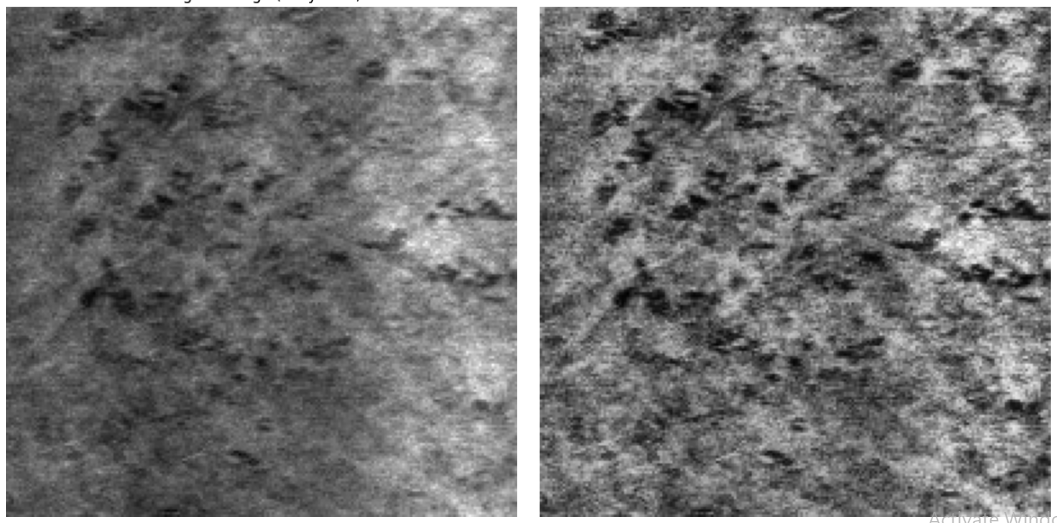
\includegraphics[width=0.9\linewidth]{img/CLAHE.png}
		\caption{تاثیر پیش‌پردازش \lr{CLAHE}}
	\end{figure}
	\begin{figure}[H]
		\centering
		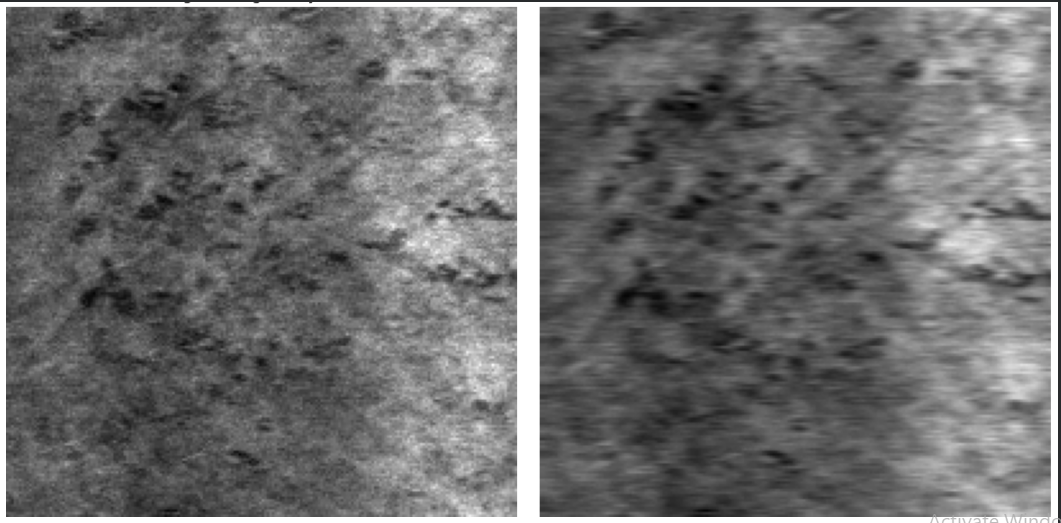
\includegraphics[width=0.9\linewidth]{img/MOTION.png}
		\caption{تاثیر پیش‌پردازش \lr{Motion Blur}}
	\end{figure}
	تصاویر سمت راست نمایانگر تصاویری هستند که بر روی آنها پیش‌پردازش‌های مذکور اعمال شده است و تصاویر سمت چپ، تصاویر خام هستند.
	
	\subsection{تبدیل برچسب‌ها از فرمت VOC به فرمت YOLO}
	
	مجموعه داده NEU-DET به‌صورت پیش‌فرض از قالب برچسب‌گذاری \lr{Pascal VOC} استفاده می‌کند که در آن، اطلاعات هر شیء شامل نام کلاس و مختصات ناحیه خرابی به‌صورت مختصات مطلق پیکسلی \((xmin, ymin, xmax, ymax)\) در فایل‌های XML ذخیره می‌شود. در مقابل، مدل‌های مبتنی بر YOLO از قالب برچسب‌گذاری متفاوتی استفاده می‌کنند که در آن، موقعیت و ابعاد جعبه مرزی به‌صورت نرمال‌شده و نسبی نسبت به ابعاد تصویر بیان می‌شود.
	
	به‌منظور سازگار‌سازی دیتاست با الزامات مدل \lr{YOLO}، یک تابع تبدیل طراحی شده است که وظیفه آن استخراج اطلاعات برچسب‌ها از فایل XML و تبدیل آن‌ها به فرمت مورد نیاز YOLO می‌باشد.
	\subsubsection*{ساختار برچسب در قالب YOLO}
	
	در قالب \lr{YOLO}، هر شیء موجود در تصویر با یک خط شامل پنج مقدار نمایش داده می‌شود:
	
	\[
	(class\_id,\; x_c,\; y_c,\; w,\; h)
	\]
	
	که در آن:
	\begin{itemize}
		\item \(class\_id\): شناسه عددی کلاس خرابی
		\item \(x_c, y_c\): مختصات مرکز جعبه مرزی، نرمال‌شده نسبت به عرض و ارتفاع تصویر
		\item \(w, h\): عرض و ارتفاع جعبه مرزی، نرمال‌شده نسبت به ابعاد تصویر
	\end{itemize}
	
	تمامی این مقادیر به‌صورت عددی در بازه \([0,1]\) تعریف می‌شوند.
	
	\subsubsection*{فرآیند استخراج اطلاعات از فایل XML}
	
	در مرحله نخست، فایل XML مربوط به هر تصویر با استفاده از ساختار درختی (\lr{XML Tree}) خوانده می‌شود. سپس برای هر شیء (Object) موجود در تصویر، نام کلاس خرابی استخراج شده و با استفاده از یک نگاشت از پیش‌تعریف‌شده (\lr{CLASS\_MAP}) به شناسه عددی متناظر تبدیل می‌شود. این نگاشت تضمین می‌کند که ترتیب کلاس‌ها در تمامی تصاویر یکسان باقی بماند.
	
	پس از آن، مختصات گوشه‌های جعبه مرزی شامل \(xmin\)، \(ymin\)، \(xmax\) و \(ymax\) استخراج می‌شوند که بیانگر موقعیت مطلق ناحیه خرابی در تصویر هستند.
	
	\subsubsection*{نرمال‌سازی مختصات جعبه مرزی}
	
	برای تبدیل مختصات از قالب VOC به \lr{YOLO}، ابتدا مختصات مرکز جعبه مرزی محاسبه می‌شود:
	
	\[
	x_c = \frac{x_{min} + x_{max}}{2 \times W}
	\]
	
	\[
	y_c = \frac{y_{min} + y_{max}}{2 \times H}
	\]
	
	که در آن \(W\) و \(H\) به‌ترتیب عرض و ارتفاع تصویر هستند.
	
	سپس عرض و ارتفاع جعبه مرزی به‌صورت زیر محاسبه و نرمال‌سازی می‌شوند:
	
	\[
	w = \frac{x_{max} - x_{min}}{W}
	\]
	
	\[
	h = \frac{y_{max} - y_{min}}{H}
	\]
	
	این نرمال‌سازی باعث می‌شود مدل YOLO مستقل از رزولوشن تصویر عمل کرده و قابلیت تعمیم به تصاویر با ابعاد متفاوت را داشته باشد.
	
	\subsubsection*{تولید فایل‌های برچسب YOLO}
	پس از محاسبه مقادیر نهایی، اطلاعات هر شیء در قالب یک رشته متنی با دقت عددی مناسب ذخیره می‌شود. هر تصویر دارای یک فایل متنی مستقل با پسوند \lr{.txt} است که در آن، هر خط متناظر با یک ناحیه خرابی در تصویر می‌باشد.
	
	این ساختار ساده و استاندارد، امکان بارگذاری سریع داده‌ها و آموزش کارآمد مدل YOLO را فراهم می‌سازد.
	
	\section{آموزش چهار مدل \lr{YOLOV}}
	\subsection{آموزش مدل \lr{YOLOV8n}}
	\begin{figure}[H]
		\centering
		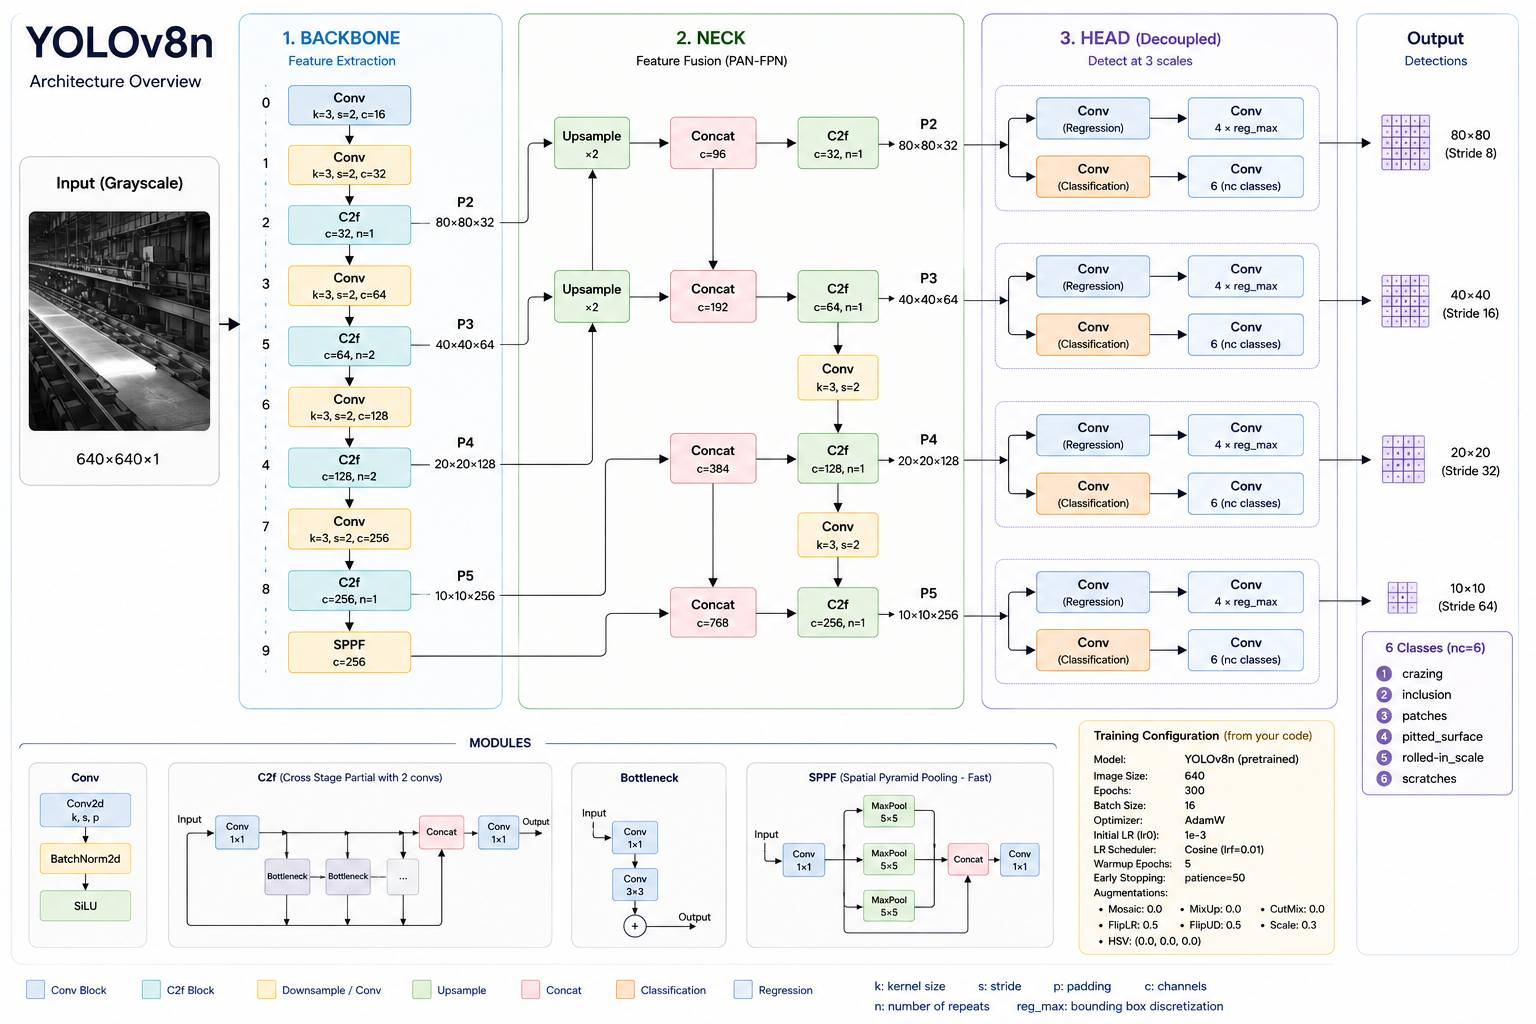
\includegraphics[width=0.9\linewidth]{img/yolov8n.png}
		\caption{ساختار مدل \lr{yolov8n} (تصویر ساخته شده با هوش مصنوعی)}
	\end{figure}
	در این مرحله، برای تشخیص عیوب سطحی از مدل آماده‌ی \lr{YOLOv8n} استفاده شده است. این مدل از خانواده‌ی \lr{YOLOv8} بوده و نسخه‌ی \lr{nano} آن محسوب می‌شود. نسخه‌ی \lr{n} نسبت به سایر نسخه‌ها مانند \lr{s}، \lr{m} و \lr{L} سبک‌تر است و تعداد پارامترهای کمتری دارد؛ بنابراین سرعت آموزش و استنتاج بالاتری دارد و برای آزمایش‌های اولیه، داده‌های محدود یا کاربردهایی که نیاز به مدل سبک دارند مناسب است.
	
	\paragraph{ساختار کلی مدل}
	مدل \lr{YOLOv8n} یک مدل تک‌مرحله‌ای \lr{One-Stage Detector} برای تشخیص شیء است. در این نوع مدل، تصویر ورودی مستقیماً وارد شبکه شده و مدل به‌صورت هم‌زمان مختصات جعبه‌های مرزی، کلاس هر شیء و میزان اطمینان پیش‌بینی را تولید می‌کند. ساختار کلی مدل شامل سه بخش اصلی است:
	
	\paragraph{بخش Backbone}
	بخش \lr{Backbone} وظیفه‌ی استخراج ویژگی‌های اولیه و عمیق از تصویر ورودی را بر عهده دارد. در این قسمت، تصویر با ابعاد مشخص وارد شبکه شده و با عبور از چندین لایه‌ی کانولوشنی، ویژگی‌هایی مانند لبه‌ها، بافت‌ها، الگوهای سطحی و نواحی دارای عیب استخراج می‌شوند. در مسئله‌ی تشخیص عیوب سطحی، این بخش اهمیت زیادی دارد؛ زیرا عیوب ممکن است کوچک، کم‌رنگ یا دارای الگوی بافتی پیچیده باشند.
	
	\paragraph{بخش Neck}
	بخش \lr{Neck} وظیفه‌ی ترکیب ویژگی‌ها در مقیاس‌های مختلف را دارد. در مدل‌های تشخیص شیء، اشیاء یا عیوب ممکن است اندازه‌های متفاوتی داشته باشند؛ بنابراین مدل باید بتواند هم ویژگی‌های ریز و محلی و هم ویژگی‌های عمیق‌تر و کلی‌تر را بررسی کند. در \lr{YOLOv8} این بخش با ترکیب ویژگی‌های چندمقیاسی باعث بهبود تشخیص عیوب کوچک و بزرگ می‌شود.
	
	\paragraph{بخش Head}
	بخش \lr{Head} خروجی نهایی مدل را تولید می‌کند. این بخش برای هر ناحیه از تصویر، مختصات جعبه‌ی مرزی، کلاس عیب و مقدار اطمینان را پیش‌بینی می‌کند. در نسخه‌های جدید \lr{YOLOv8}، ساختار \lr{Head} به‌صورت \lr{anchor-free} طراحی شده است؛ یعنی مدل برخلاف نسخه‌های قدیمی‌تر YOLO وابستگی مستقیم به \lr{anchor}های از پیش تعریف‌شده ندارد. این موضوع باعث ساده‌تر شدن فرآیند آموزش و افزایش انعطاف‌پذیری مدل در تشخیص اشیاء با شکل‌ها و اندازه‌های مختلف می‌شود.
	
	\paragraph{استفاده از وزن‌های از پیش آموزش‌دیده}
	
	فایل \lr{yolov8n.pt} شامل وزن‌های از پیش آموزش‌دیده‌ی مدل است. این وزن‌ها معمولاً روی یک دیتاست بزرگ عمومی مانند \lr{COCO} آموزش دیده‌اند. استفاده از این وزن‌ها باعث می‌شود مدل آموزش را از یک نقطه‌ی اولیه‌ی مناسب آغاز کند، نه از وزن‌های تصادفی.
	
	\paragraph{تنظیمات داده}
	
	در فایل \lr{data.yaml} مسیر تصاویر آموزشی و اعتبارسنجی، تعداد کلاس‌ها و نام کلاس‌ها تعریف می‌شود. مدل در زمان آموزش از این فایل استفاده می‌کند تا بداند داده‌های آموزشی در چه مسیری قرار دارند و مسئله شامل چند کلاس است.
	
	\paragraph{تعداد دوره‌های آموزش}
	یعنی مدل حداکثر به مدت ۳۰۰ epoch روی داده‌ها آموزش داده می‌شود. در هر \lr{epoch}، مدل کل داده‌های آموزشی را یک بار مشاهده می‌کند. انتخاب مقدار ۳۰۰ باعث می‌شود مدل فرصت کافی برای یادگیری الگوهای عیوب سطحی داشته باشد.
	
	\paragraph{اندازه تصویر ورودی}
	
	در این حالت تصاویر قبل از ورود به مدل به ابعاد $640 \times 640$ تبدیل می‌شوند. این اندازه یکی از مقادیر رایج در آموزش مدل‌های YOLO است و تعادل مناسبی بین دقت و سرعت ایجاد می‌کند.
	
	\paragraph{اندازه Batch} 
	در این آموزش، در هر iteration تعداد ۱۶ تصویر به مدل داده می‌شود.
	
	\paragraph{بهینه‌ساز و نرخ یادگیری}
	در این آموزش از بهینه‌ساز \lr{AdamW} استفاده شده است:
	
	بهینه‌ساز \lr{AdamW} نسخه‌ای بهبود‌یافته از \lr{Adam} است که در آن تنظیم وزن‌ها و کاهش بیش‌برازش بهتر کنترل می‌شود. مقدار اولیه‌ی نرخ یادگیری برابر با $10^{-3}$ در نظر گرفته شده است. همچنین پارامتر \lr{lrf} مقدار نهایی نسبی نرخ یادگیری را مشخص می‌کند؛ یعنی نرخ یادگیری در انتهای آموزش نسبت به مقدار اولیه کاهش می‌یابد.
	
	\paragraph{زمان‌بندی نرخ یادگیری}
	
	با فعال بودن \lr{cos\_lr}، نرخ یادگیری در طول آموزش به‌صورت تدریجی و نرم کاهش می‌یابد. این کار باعث پایدارتر شدن آموزش در \lr{epoch}های پایانی می‌شود. همچنین در ۵ epoch ابتدایی، فرآیند \lr{warmup} انجام می‌شود؛ یعنی نرخ یادگیری به‌آرامی افزایش می‌یابد تا از ناپایداری آموزش در ابتدای کار جلوگیری شود.
	
	\paragraph{تنظیمات افزایش داده}
	
	روش‌های \lr{Mosaic}، \lr{MixUp} و \lr{CutMix} برای ترکیب تصاویر و ایجاد نمونه‌های مصنوعی استفاده می‌شوند. در اینجا مقدار آن‌ها صفر قرار داده شده است؛ بنابراین این روش‌ها اعمال نمی‌شوند. چون ما نیازی به تولید دیتای مصنوعی نداشتیم و هدفمان این بود که مدل بر روی دیتاهای واقعی آموزش ببیند و ارزیابی شود.
	
	پارامتر \lr{fliplr=0.5} یعنی تصاویر با احتمال ۵۰ درصد به‌صورت افقی برگردانده می‌شوند. همچنین \lr{flipud=0.5} باعث وارون‌سازی عمودی تصاویر با احتمال ۵۰ درصد می‌شود. پارامتر \lr{scale=0.3} نیز تغییر مقیاس تصویر را اعمال می‌کند. این تبدیلات باعث افزایش تنوع داده‌های آموزشی و کاهش احتمال بیش‌برازش می‌شوند.
	
	\paragraph{توقف زودهنگام}
	اگر عملکرد مدل روی داده‌های اعتبارسنجی به مدت ۵۰ epoch بهتر نشود، فرآیند آموزش متوقف می‌شود. این کار از ادامه‌ی آموزش غیرضروری جلوگیری کرده و احتمال بیش‌برازش را کاهش می‌دهد.
	
	\paragraph{جمع‌بندی}
	در مجموع، در این پیاده‌سازی از مدل سبک و سریع \lr{YOLOv8n} همراه با وزن‌های از پیش آموزش‌دیده استفاده شده است. مدل با روش \lr{Transfer Learning} روی دیتاست هدف آموزش داده می‌شود. تنظیمات آموزش شامل ۳۰۰ epoch، اندازه تصویر $640 \times 640$، batch برابر با ۱۶، بهینه‌ساز \lr{AdamW}، نرخ یادگیری اولیه $10^{-3}$ و زمان‌بندی کسینوسی است. همچنین برای حفظ ویژگی‌های واقعی تصاویر صنعتی، روش‌های ترکیبی مانند \lr{Mosaic}، \lr{MixUp} و \lr{CutMix} و تغییرات رنگی غیرفعال شده‌اند، اما تبدیلات هندسی مانند چرخش افقی، عمودی و تغییر مقیاس برای افزایش تنوع داده‌ها استفاده شده‌اند.
	
	در ادامه نتایج مربوط به ارزیابی این مدل ارائه می گردد و سپس روی این نتایج تحلیل انجام می شود:
	\subsection{تحلیل نتایج آموزش مدل \lr{YOLOv8n}}
	\begin{figure}[H]
		\centering
		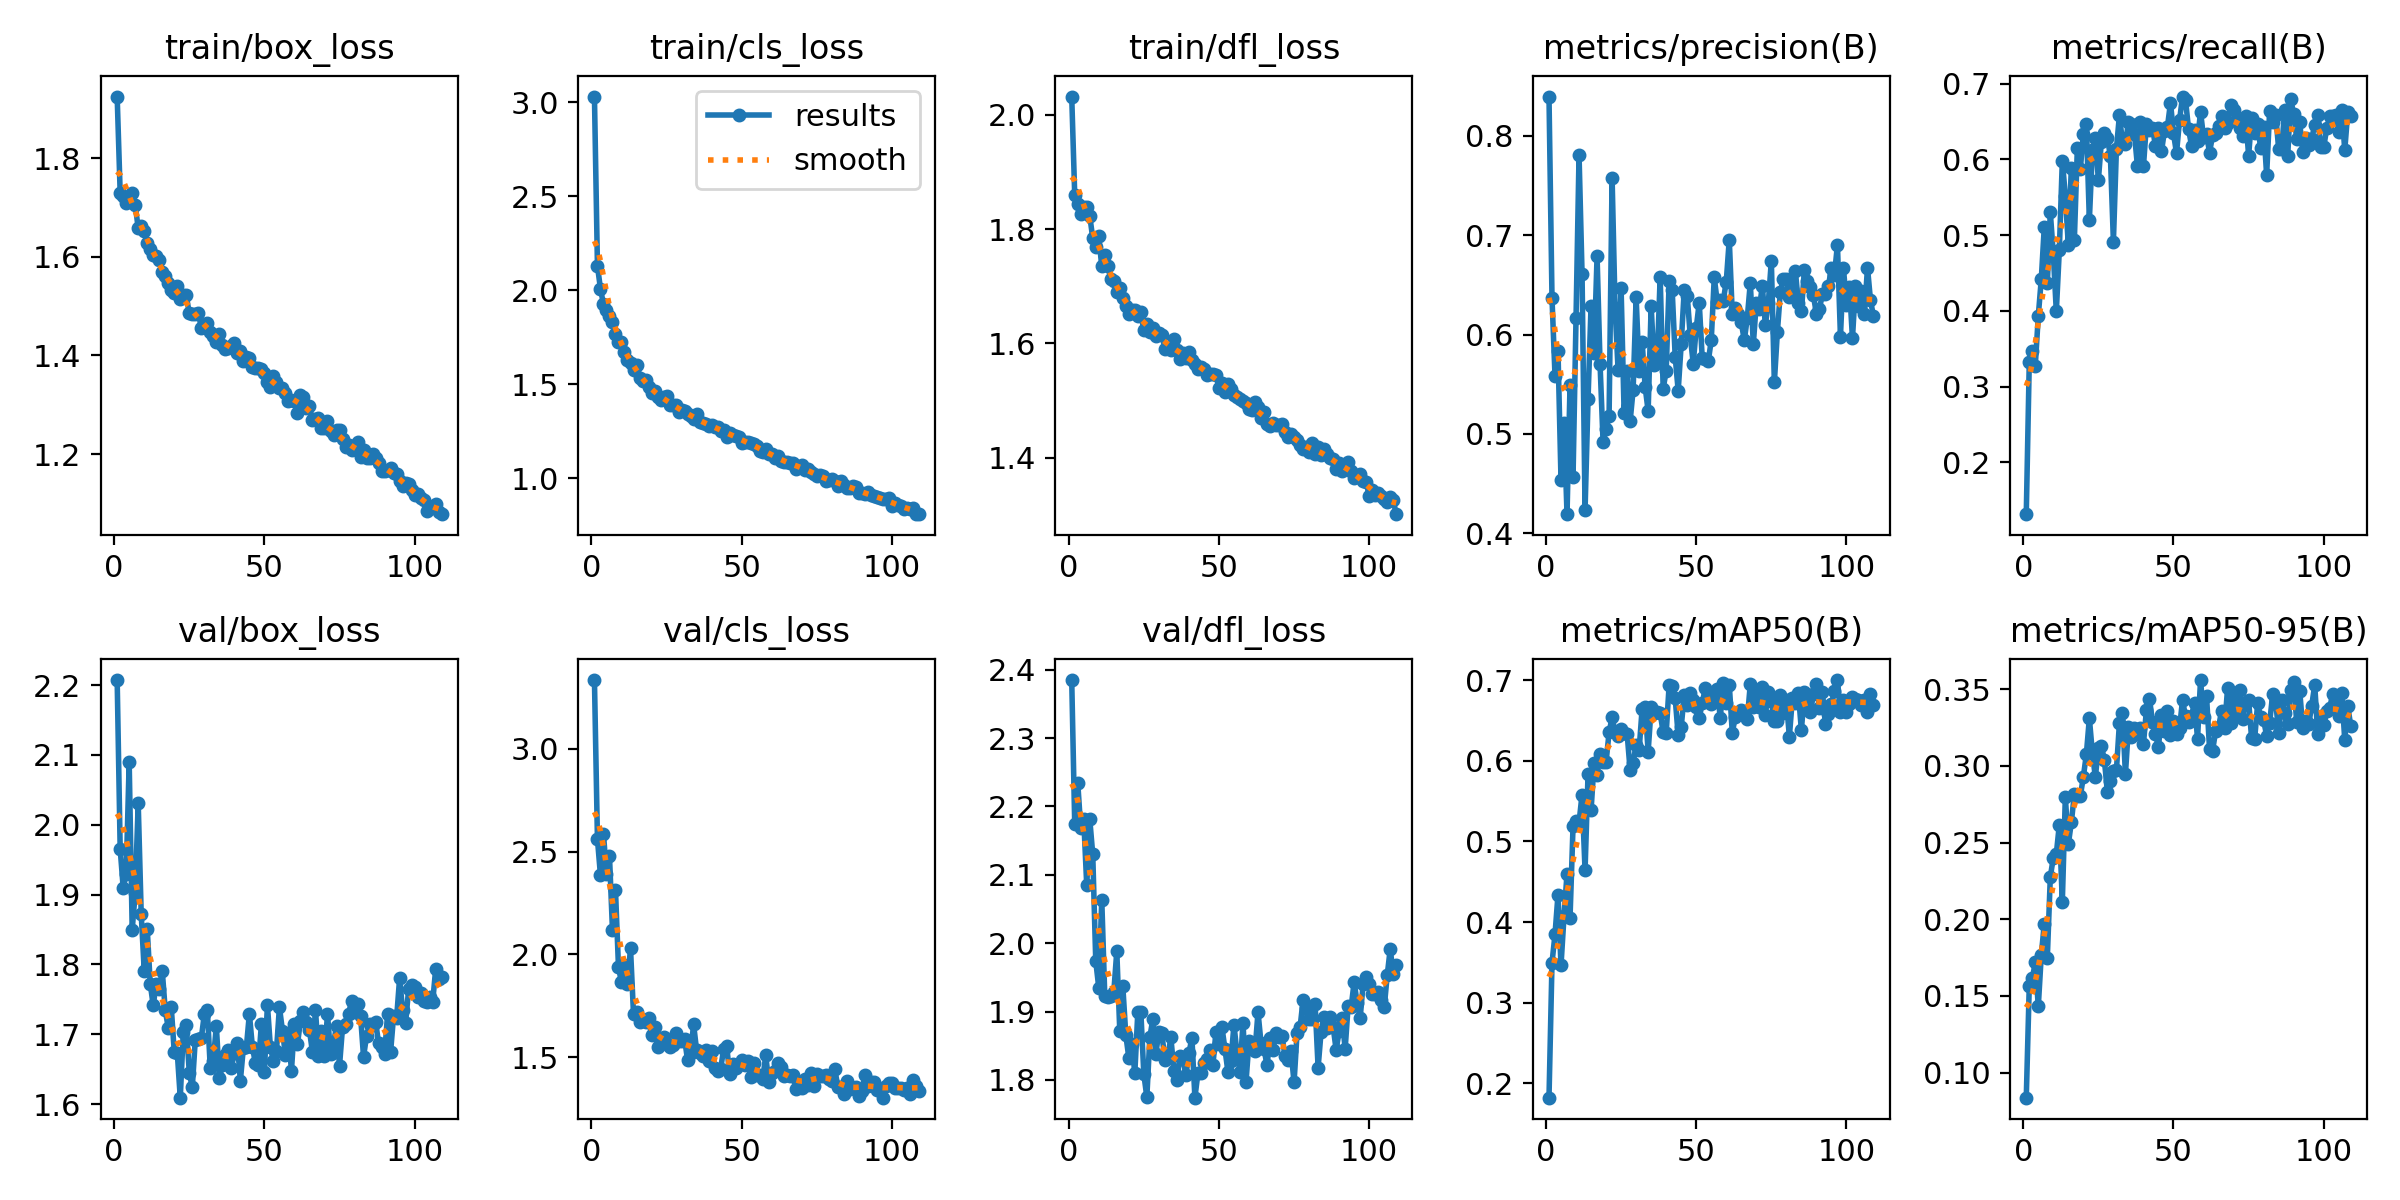
\includegraphics[width=0.9\linewidth]{img/resultsyolov8n.png}
		\caption{نمودارهای مربوط به روند آموزش مدل}
	\end{figure}
	
	
	شکل بالا  روند تغییر توابع خطا و معیارهای ارزیابی مدل را در \lr{epoch}های مختلف نمایش می‌دهند.
	
	با وجود آن‌که حداکثر تعداد epoch برابر با 300 در نظر گرفته شده بود، نمودارها نشان می‌دهند آموزش تقریباً در epoch $110$ متوقف شده است. این اتفاق به خاطر فعال بودن مکانیزم توقف زودهنگام با مقدار \lr{patience=50} است؛ یعنی معیار ارزیابی مدل در مجموعه اعتبارسنجی طی تعداد مشخصی epoch بهبود مؤثری نداشته و آموزش برای جلوگیری از بیش‌برازش متوقف شده است. این درحالیست که مدل هایی که با تغییرات ساختاری آموزش دادیم، تا 300 \lr{epoch} آموزش دیدند و کمتر دچار بیش برازش شدند(در \lr{Yolov8n-Improvement} دچار بیش برازش نشدیم).
	
	\paragraph{تحلیل خطای مکان‌یابی در داده‌های آموزش}
	
	نمودار \lr{train/box\_loss} مربوط به خطای پیش‌بینی جعبه‌های مرزی است. این خطا از حدود $1.9$ در ابتدای آموزش شروع شده و به‌صورت پیوسته تا حدود $1.08$ در انتهای آموزش کاهش یافته است. کاهش یکنواخت این منحنی نشان می‌دهد مدل به‌تدریج توانایی بهتری در تعیین موقعیت و ابعاد ناحیه‌ی عیب روی سطح فولاد پیدا کرده است.
	البته باید گفت که خطای استنتاج روی داده های اعتبارسنجی همواره نزولی نبوده و دچار بیش برازش شدیم.
	\paragraph{تحلیل خطای طبقه‌بندی در داده‌های آموزش}
	
	نمودار \lr{train/cls\_loss} خطای مربوط به تشخیص کلاس عیب را نمایش می‌دهد. مقدار این خطا از حدود $3.0$ در ابتدای آموزش به حدود $0.8$ در انتهای فرآیند کاهش یافته است. این کاهش قابل توجه بیانگر آن است که مدل در تفکیک تدریجی کلاس‌های مختلف عیب عملکرد بهتری پیدا کرده است.
	
	با این حال، ماهیت برخی از کلاس‌های دیتاست \lr{NEU} می‌تواند باعث دشوار شدن طبقه‌بندی شود. برای نمونه، عیوب \lr{Patches}، \lr{Inclusion} و \lr{Pitted Surface} ممکن است در برخی تصاویر دارای بافت‌ها یا نواحی ظاهری نزدیک به هم باشند.
	
	\paragraph{تحلیل خطای \lr{DFL} در داده‌های آموزش}
	
	نمودار \lr{train/dfl\_loss} به خطای \lr{Distribution Focal Loss} مربوط است. این مؤلفه در \lr{YOLOv8} برای دقیق‌تر شدن پیش‌بینی مختصات جعبه‌های مرزی استفاده می‌شود. مقدار این خطا از حدود $2.0$ به نزدیک $1.3$ کاهش یافته است. کاهش پیوسته‌ی این نمودار در کنار کاهش \lr{train/box\_loss} نشان می‌دهد که مدل نه‌تنها مکان تقریبی عیب، بلکه مرزهای جعبه‌ی پیرامون عیب را نیز با دقت بهتری تخمین زده است.
	
	\paragraph{تحلیل خطاهای مجموعه اعتبارسنجی}
	
	نمودارهای \lr{val/box\_loss}، \lr{val/cls\_loss} و \lr{val/dfl\_loss} معیار مهمی برای بررسی قابلیت تعمیم مدل به تصاویر دیده‌نشده هستند.
	
	مقدار \lr{val/box\_loss} ابتدا از حدود $2.2$ به نزدیک $1.65$ کاهش پیدا کرده است؛ اما پس از تقریباً \lr{epoch} $25$ تا $35$ \lr{epoch}، روند آن تقریباً ثابت شده و در \lr{epoch}های پایانی مقداری افزایش یافته است. مقدار نهایی این خطا حدود $1.75$ تا $1.78$ است. این رفتار نشان می‌دهد مدل در ابتدای آموزش به‌سرعت در مکان‌یابی عیوب روی داده‌های اعتبارسنجی پیشرفت کرده، اما ادامه‌ی آموزش باعث بهبود قابل توجهی در تعمیم مکان‌یابی نشده است.
	
	رفتار \lr{val/dfl\_loss} نیز مشابه است. این خطا ابتدا کاهش پیدا کرده و کمینه‌ای در حدود $1.80$ تا $1.82$ دارد، اما در ادامه به سمت حدود $1.95$ افزایش یافته است. افزایش هم‌زمان \lr{val/box\_loss} و \lr{val/dfl\_loss} در مراحل انتهایی آموزش، می‌تواند نشانه‌ای از آغاز بیش‌برازش در بخش مکان‌یابی باشد. به عبارت دیگر، مدل همچنان روی داده‌های آموزش بهتر می‌شود، اما این بهبود به همان اندازه به داده‌های اعتبارسنجی منتقل نمی‌شود.
	
	در مقابل، \lr{val/cls\_loss} از حدود $3.35$ در ابتدای آموزش به نزدیک $1.35$ در انتها کاهش یافته و در \lr{epoch}های پایانی تقریباً پایدار شده است. این موضوع نشان می‌دهد که قابلیت طبقه‌بندی عیوب در داده‌های اعتبارسنجی به‌طور کلی مناسب است و بیش‌برازش مشاهده‌شده بیشتر به بخش تعیین دقیق مرزهای عیب مربوط می‌شود تا تشخیص نوع عیب.
	
	\paragraph{تحلیل معیار \lr{Precision}}
	
	مقدار \lr{Precision} در \lr{epoch}های ابتدایی دارای نوسان نسبتاً زیادی است، اما پس از حدود epoch $30$ روند پایدارتری پیدا می‌کند و در محدوده‌ی تقریبی $0.62$ تا $0.67$ قرار می‌گیرد. مقدار نهایی precision تقریباً برابر با $0.64$ است.
	
	معیار precision از رابطه‌ی زیر تعریف می‌شود:
	
	\begin{latin}
		\begin{equation}
			\text{Precision} =
			\frac{TP}{TP + FP},
		\end{equation}
	\end{latin}
	
	که در آن $TP$ تعداد تشخیص‌های صحیح و $FP$ تعداد تشخیص‌های اشتباه است. مقدار precision حدود $0.64$ بیان می‌کند که بخش قابل توجهی از جعبه‌های پیش‌بینی‌شده توسط مدل درست هستند، اما همچنان تعدادی تشخیص مثبت کاذب وجود دارد. این موارد می‌توانند ناشی از شباهت بافت بخش‌های سالم سطح فولاد با الگوهای برخی عیوب، یا شباهت ظاهری میان کلاس‌های مختلف عیب باشند.
	
	\paragraph{تحلیل معیار \lr{Recall}}
	
	نمودار \lr{Recall} در ابتدای آموزش رشد سریعی دارد و از حدود $0.13$ به محدوده‌ی $0.60$ می‌رسد. پس از آن نیز تقریباً در بازه‌ی $0.62$ تا $0.66$ پایدار می‌شود. مقدار نهایی recall حدود $0.64$ است.
	
	معیار recall به‌صورت زیر تعریف می‌شود:
	
	\begin{latin}
		\begin{equation}
			\text{Recall} =
			\frac{TP}{TP + FN},
		\end{equation}
	\end{latin}
	
	که در آن $FN$ بیانگر عیوبی است که در تصویر وجود داشته‌اند، اما توسط مدل شناسایی نشده‌اند. مقدار recall نزدیک به $0.64$ نشان می‌دهد مدل تقریباً بخش قابل قبولی از عیوب موجود را پیدا می‌کند، ولی هنوز بخشی از عیوب، به‌ویژه عیوب کوچک، کم‌کنتراست یا دارای مرز نامشخص، ممکن است از دید مدل پنهان بمانند.
	
	نزدیک بودن مقادیر precision و recall یک نکته‌ی مثبت محسوب می‌شود؛ زیرا نشان می‌دهد مدل میان تولید تشخیص‌های اشتباه و از دست دادن عیوب واقعی، توازن نسبی برقرار کرده است.
	
	\paragraph{تحلیل معیار \lr{mAP@50}}
	
	نمودار \lr{metrics/mAP50(B)} رشد سریعی در \lr{epoch}های ابتدایی دارد. مقدار این معیار از حدود $0.18$ آغاز شده و بعد از حدود 30 تا 40 epoch به بازه‌ی $0.65$ تا $0.69$ می‌رسد. سپس با نوسان محدود، تقریباً در همین محدوده باقی می‌ماند. مقدار نهایی \lr{mAP@50} نزدیک به $0.68$ است.
	
	معیار \lr{mAP@50} میانگین دقت متوسط کلاس‌ها در آستانه‌ی هم‌پوشانی $\mathrm{IoU}=0.5$ را اندازه‌گیری می‌کند. به‌صورت مفهومی، اگر هم‌پوشانی جعبه‌ی پیش‌بینی‌شده و جعبه‌ی واقعی حداقل برابر با $0.5$ باشد، تشخیص صحیح در نظر گرفته می‌شود. مقدار نزدیک به $0.68$ نشان می‌دهد مدل در تشخیص کلی شش نوع عیب سطحی، عملکرد قابل قبول و نسبتاً مناسبی دارد.
	
	همچنین، پایدار شدن این منحنی پس از حدود epoch $40$ تا $50$ نشان می‌دهد بخش عمده‌ی ظرفیت یادگیری مدل در همان مراحل میانی آموزش استفاده شده است. به همین دلیل، افزایش تعداد epochها پس از این مرحله بهبود چشمگیری در \lr{mAP@50} ایجاد نکرده است.
	
	\paragraph{تحلیل معیار \lr{mAP@50-95}}
	
	معیار \lr{mAP@50-95} سخت‌گیرانه‌تر از \lr{mAP@50} است؛ زیرا میانگین عملکرد مدل را در آستانه‌های مختلف \lr{IoU} از $0.5$ تا $0.95$ محاسبه می‌کند. مقدار این معیار در نتایج حاضر از حدود $0.08$ به نزدیک $0.33$ تا $0.34$ افزایش یافته است.
	
	\begin{latin}
		\begin{equation}
			\text{mAP@50-95} =
			\frac{1}{10}
			\sum_{\mathrm{IoU}=0.50}^{0.95}
			\text{AP}_{\mathrm{IoU}}.
		\end{equation}
	\end{latin}
	
	اختلاف میان \lr{mAP@50} نزدیک به $0.68$ و \lr{mAP@50-95} نزدیک به $0.33$ نشان می‌دهد مدل در تشخیص ناحیه‌ی کلی عیب موفق‌تر از تعیین مرز کاملاً دقیق آن است. این نتیجه با روند افزایشی \lr{val/box\_loss} و \lr{val/dfl\_loss} در epochهای پایانی نیز سازگار است.
	
	این موضوع در دیتاست \lr{NEU Surface Defect Database} قابل انتظار است؛ زیرا برخی عیوب دارای مرزهای نامشخص، پراکنده یا نامنظم هستند. بنابراین، مدل غالباً قادر به تشخیص وجود عیب است(هر چند که در مقابل مدل های دیگر خطای بیشتری در تشخیص عیوب کلاس ها دارد)، اما در انطباق کاملاً دقیق جعبه‌ی پیش‌بینی‌شده با ناحیه‌ی واقعی عیب، با چالش مواجه می‌شود.
	
	\paragraph{جمع‌بندی تحلیل}
	
	نتایج نشان می‌دهند مدل \lr{YOLOv8n} توانسته است الگوهای اصلی شش عیب سطحی دیتاست \lr{NEU} را فرا بگیرد. کاهش یکنواخت خطاهای آموزشی و رشد سریع معیارهای \lr{mAP}، precision و recall نشان‌دهنده‌ی همگرایی مناسب مدل در طول فرآیند آموزش است.
	
	مقادیر تقریبی نهایی معیارها به‌صورت زیر قابل جمع‌بندی هستند:
	
	\begin{latin}
		\begin{equation}
			\text{Precision} \approx 0.64,
			\qquad
			\text{Recall} \approx 0.64,
			\qquad
			\text{mAP@50} \approx 0.68,
			\qquad
			\text{mAP@50-95} \approx 0.33.
		\end{equation}
	\end{latin}
	
	اگرچه عملکرد مدل از نظر تشخیص کلی عیوب قابل قبول است، افزایش تدریجی خطاهای مکانیابی در داده‌های اعتبارسنجی پس از رسیدن به کمینه، نشان‌دهنده‌ی وجود بیش‌برازش در مراحل پایانی آموزش است. در مدل های پیش رو تلاش می کنیم تا این ایراد را برطرف نماییم.
	\subsubsection*{تحلیل ماتریس درهم‌ریختگی}
	
	\begin{figure}[H]
		\centering
		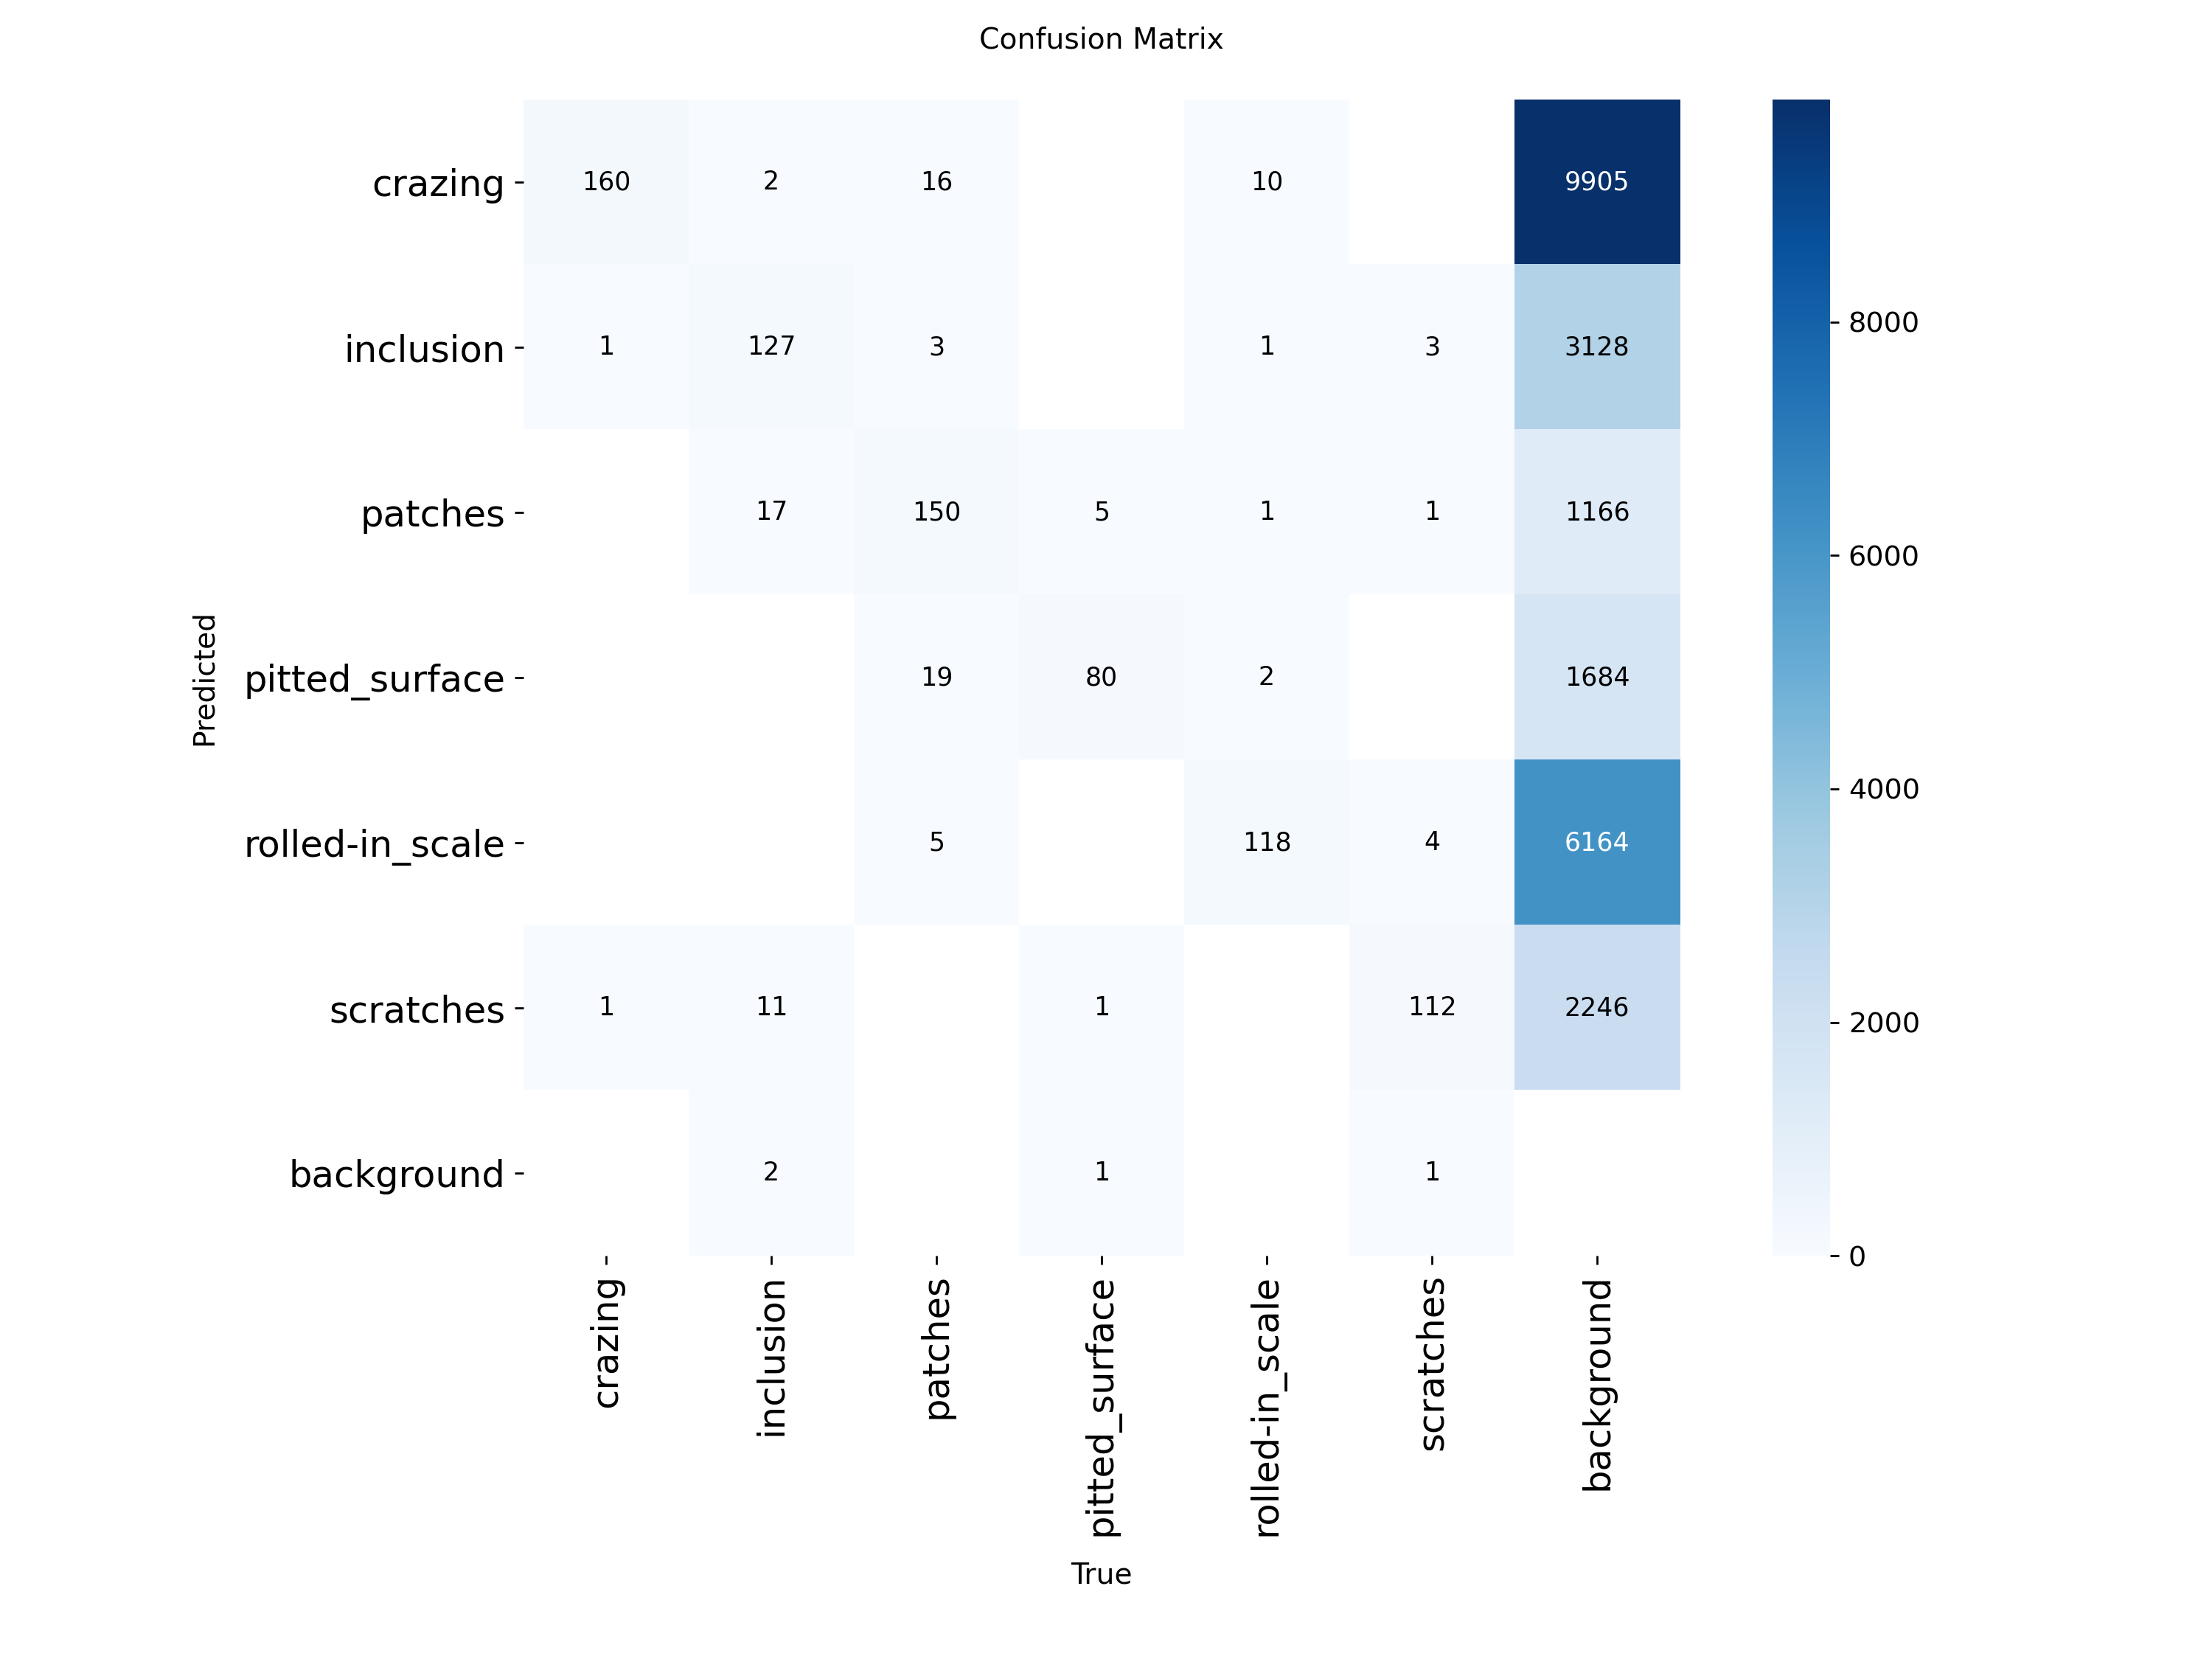
\includegraphics[width=0.45\linewidth]{img/confusionmatrixyolov8n.png}
		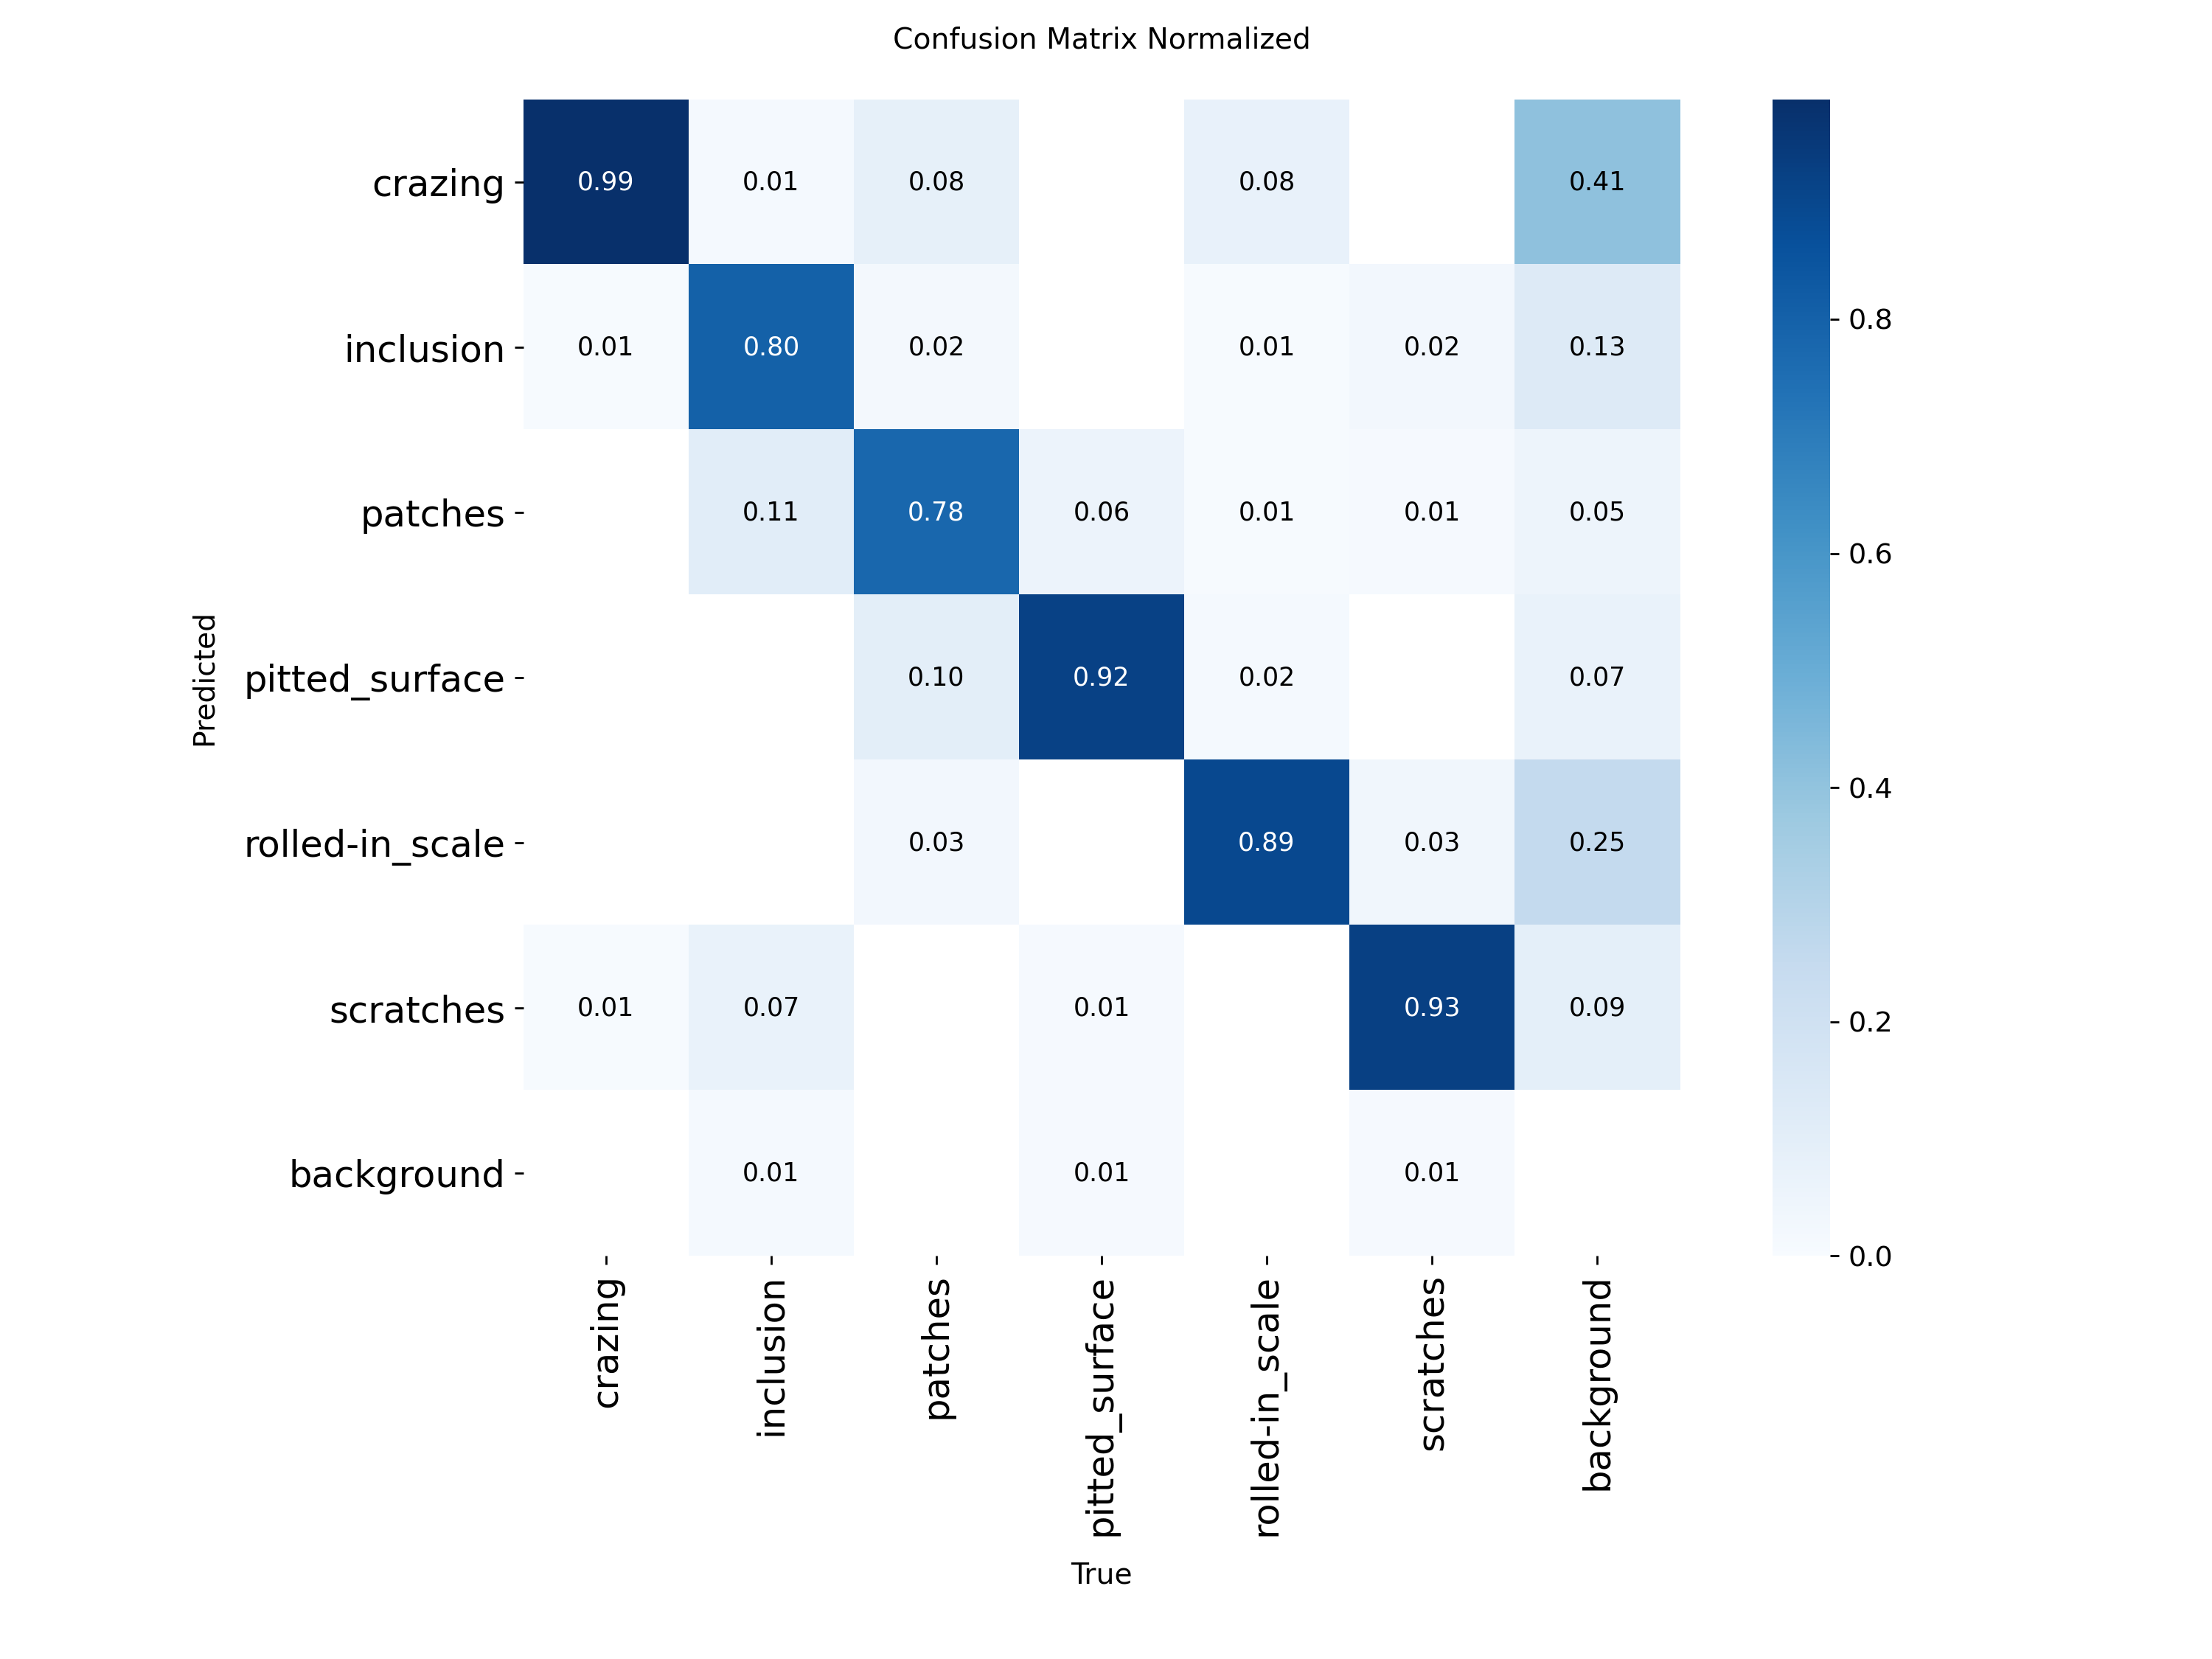
\includegraphics[width=0.45\linewidth]{img/confusion_matrix_normalized8n.png}
		\caption{ماتریس درهمریختگی}
	\end{figure}
	
	ماتریس درهم‌ریختگی نشان می‌دهد که مدل \lr{YOLOv8n} در تشخیص کلاس‌های اصلی دیتاست \lr{NEU Surface Defect Database} عملکرد بدی نداشته است، زیرا بیشترین مقادیر درایه‌ها روی قطر اصلی قرار دارند. این موضوع بیان می‌کند که مدل در بسیاری از نمونه‌ها توانسته است عیب واقعی را به‌درستی شناسایی کند.
	
	\paragraph{خطاهای بین‌کلاسی و پس‌زمینه}
	با این حال، نتایج ماتریس نشان می‌دهند که خطای مدل فقط به اشتباه با \lr{background} محدود نبوده است، بلکه میان برخی کلاس‌های عیب نیز درهم‌ریختگی مشاهده می‌شود. برای مثال، بخشی از نمونه‌های \lr{Patches} با \lr{Crazing} یا \lr{Pitted Surface}، و برخی نمونه‌های \lr{Scratches} یا \lr{Rolled-in Scale} نیز با سایر کلاس‌های دارای الگوهای بافتی نزدیک اشتباه گرفته شده‌اند. این موضوع نشان می‌دهد که مدل پایه در تفکیک دقیق عیوبی که از نظر ظاهری شباهت بافتی یا ساختاری دارند، هنوز با محدودیت مواجه بوده است.
	
	علاوه بر این، مقادیر نسبتاً زیاد در ستون یا سطر مربوط به \lr{background} نیز نشان می‌دهد که مدل در برخی موارد یا عیب واقعی را از دست داده و آن را پس‌زمینه در نظر گرفته است، یا برعکس، نواحی غیرعیب را به‌عنوان یکی از کلاس‌ها پیش‌بینی کرده است. بنابراین، مسئله‌ی مدل پایه فقط خطای تشخیص پس‌زمینه نیست، بلکه بخشی از ضعف آن به اشتباهات بین‌کلاسی نیز مربوط می‌شود.
	
	\paragraph{مدل‌های سفارشی‌سازی‌شده}
	این الگوی خطا یکی از دلایل اصلی حرکت به سمت مدل‌های سفارشی‌سازی‌شده در مراحل بعدی بوده است. در نسخه‌های بعدی که معماری مدل تغییر داده شد و از ساختارهای بهتری استفاده شد، این مشکل تا حد زیادی کاهش یافت؛ به‌طوری‌که مدل توانست مرز بهتری میان کلاس‌های مشابه ایجاد کند و خطاهای بین‌کلاسی را کمتر کند.
	
	\subsubsection*{تحلیل منحنی‌های ارزیابی مدل}
	
	شکل زیر عملکرد مدل را در آستانه‌های مختلف \lr{Confidence} نشان می‌دهد. این منحنی‌ها شامل \lr{Precision}، \lr{Recall}، \lr{F1-score} و \lr{Precision--Recall} هستند و برای ارزیابی تعادل میان تشخیص‌های صحیح، از دست‌رفتن عیوب و پیش‌بینی‌های اشتباه استفاده می‌شوند.
	
	\begin{figure}[ht]
		\centering
		
		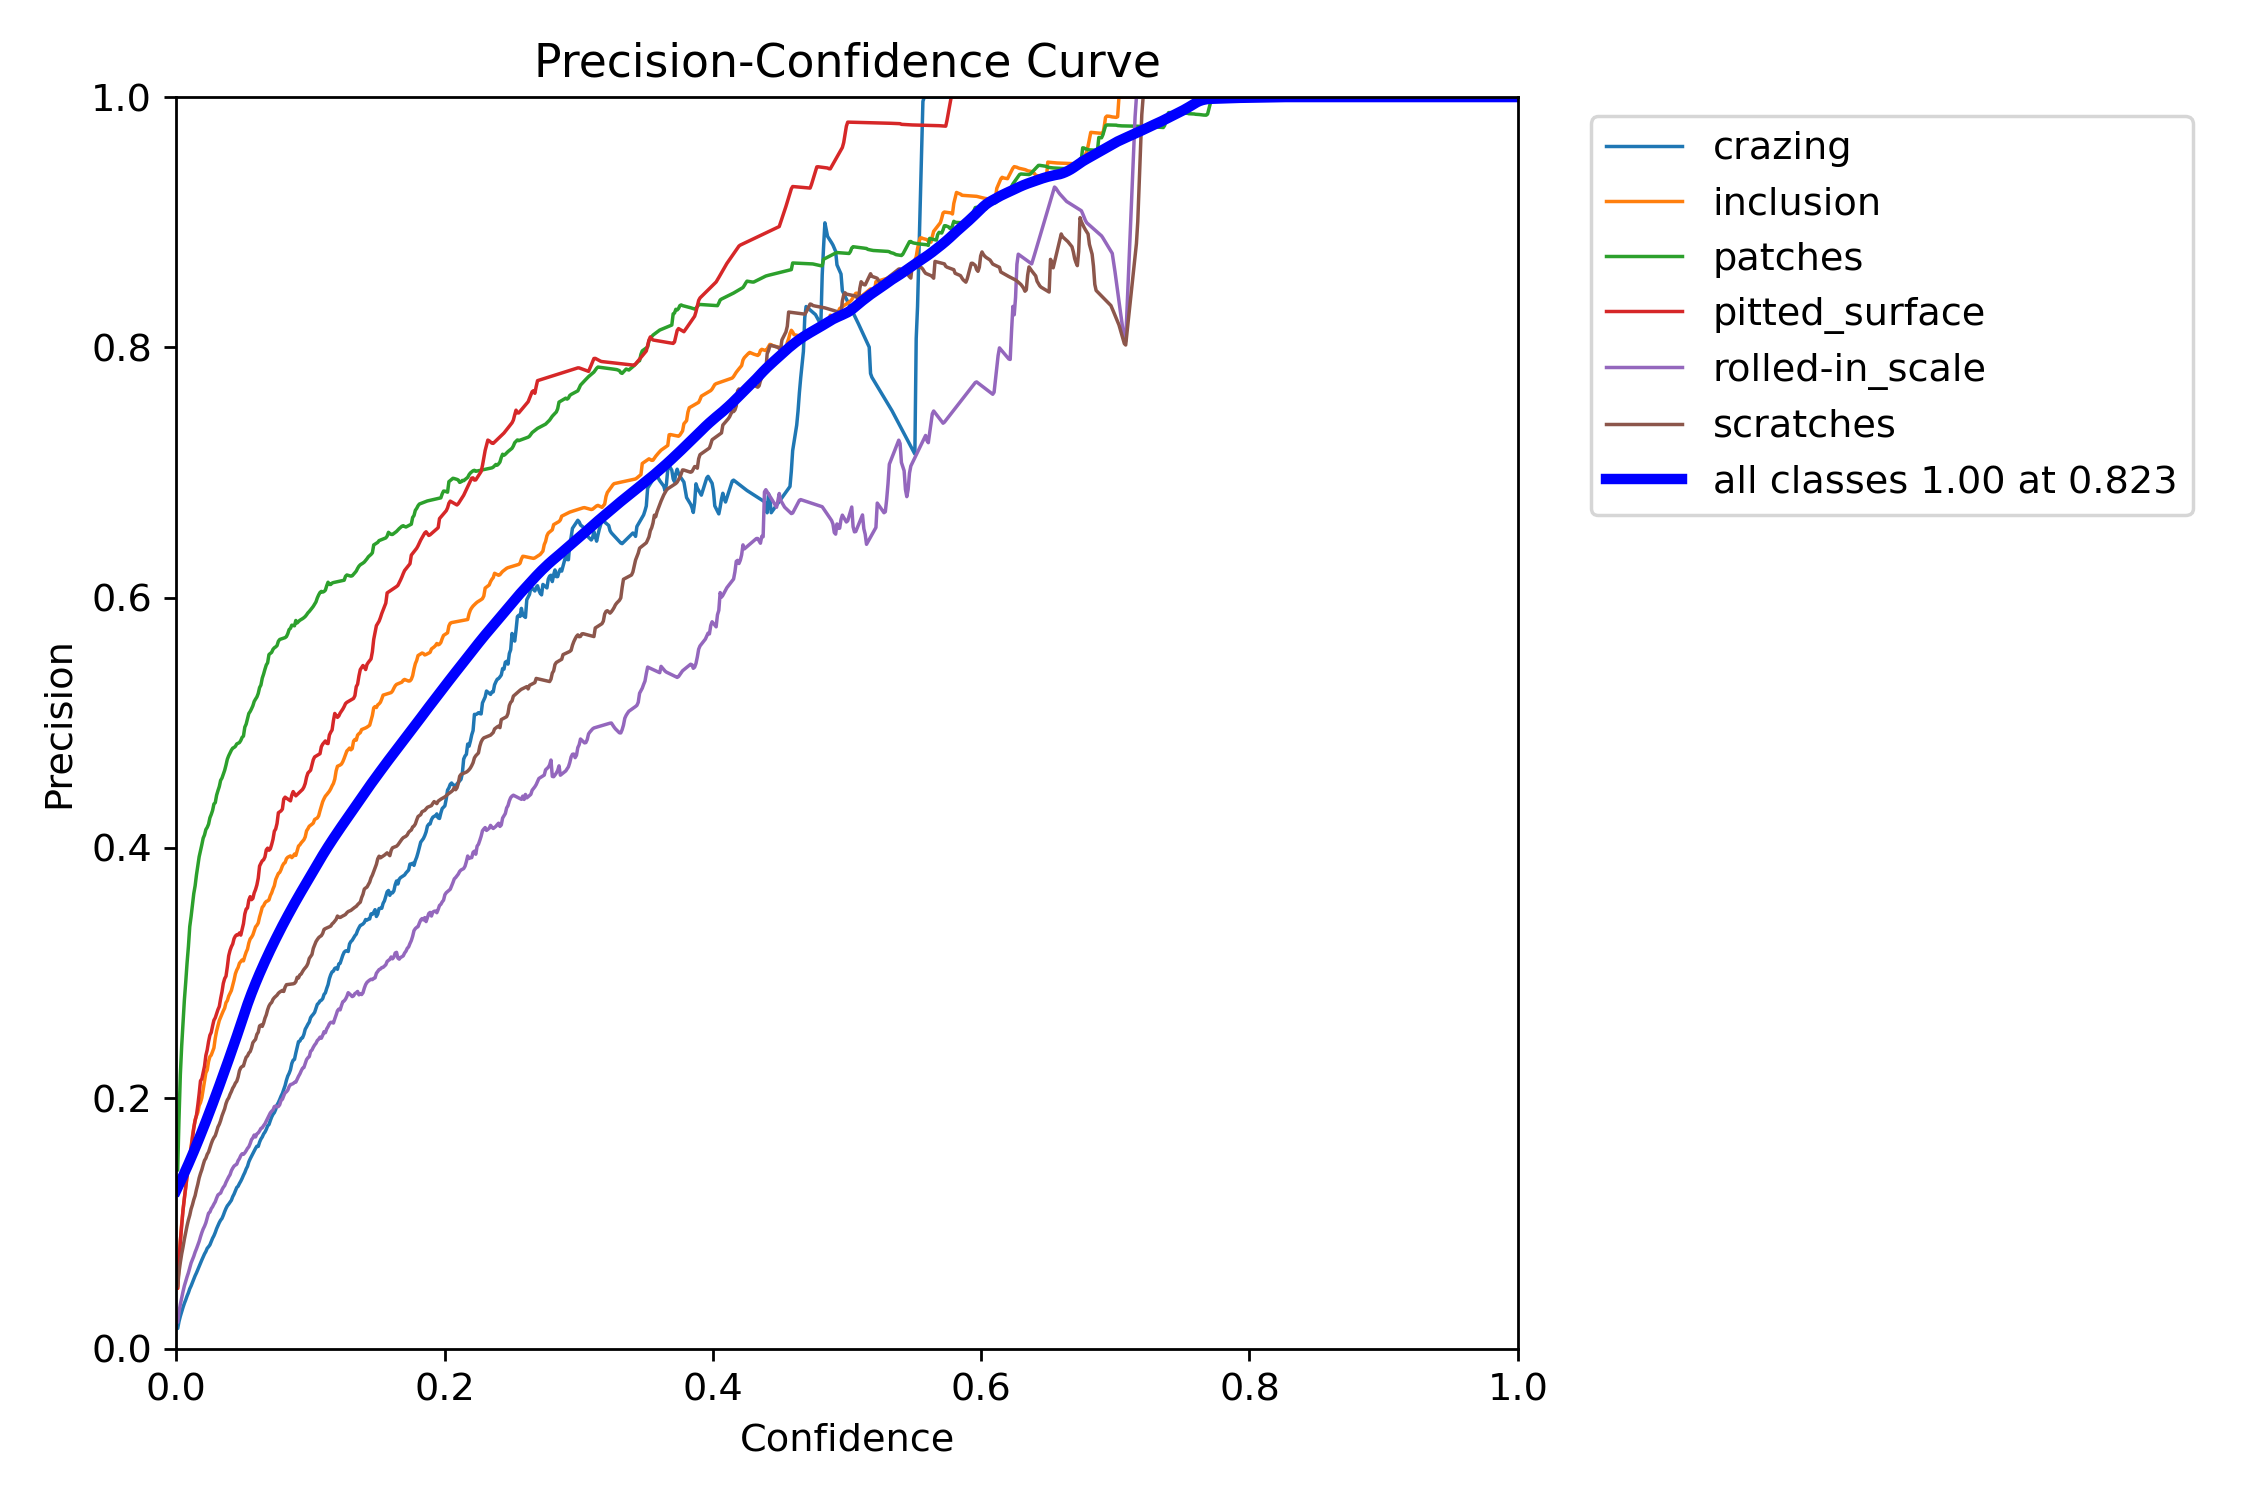
\includegraphics[width=0.46\linewidth]{img/BoxP_curve8n.png}
		\hfill
		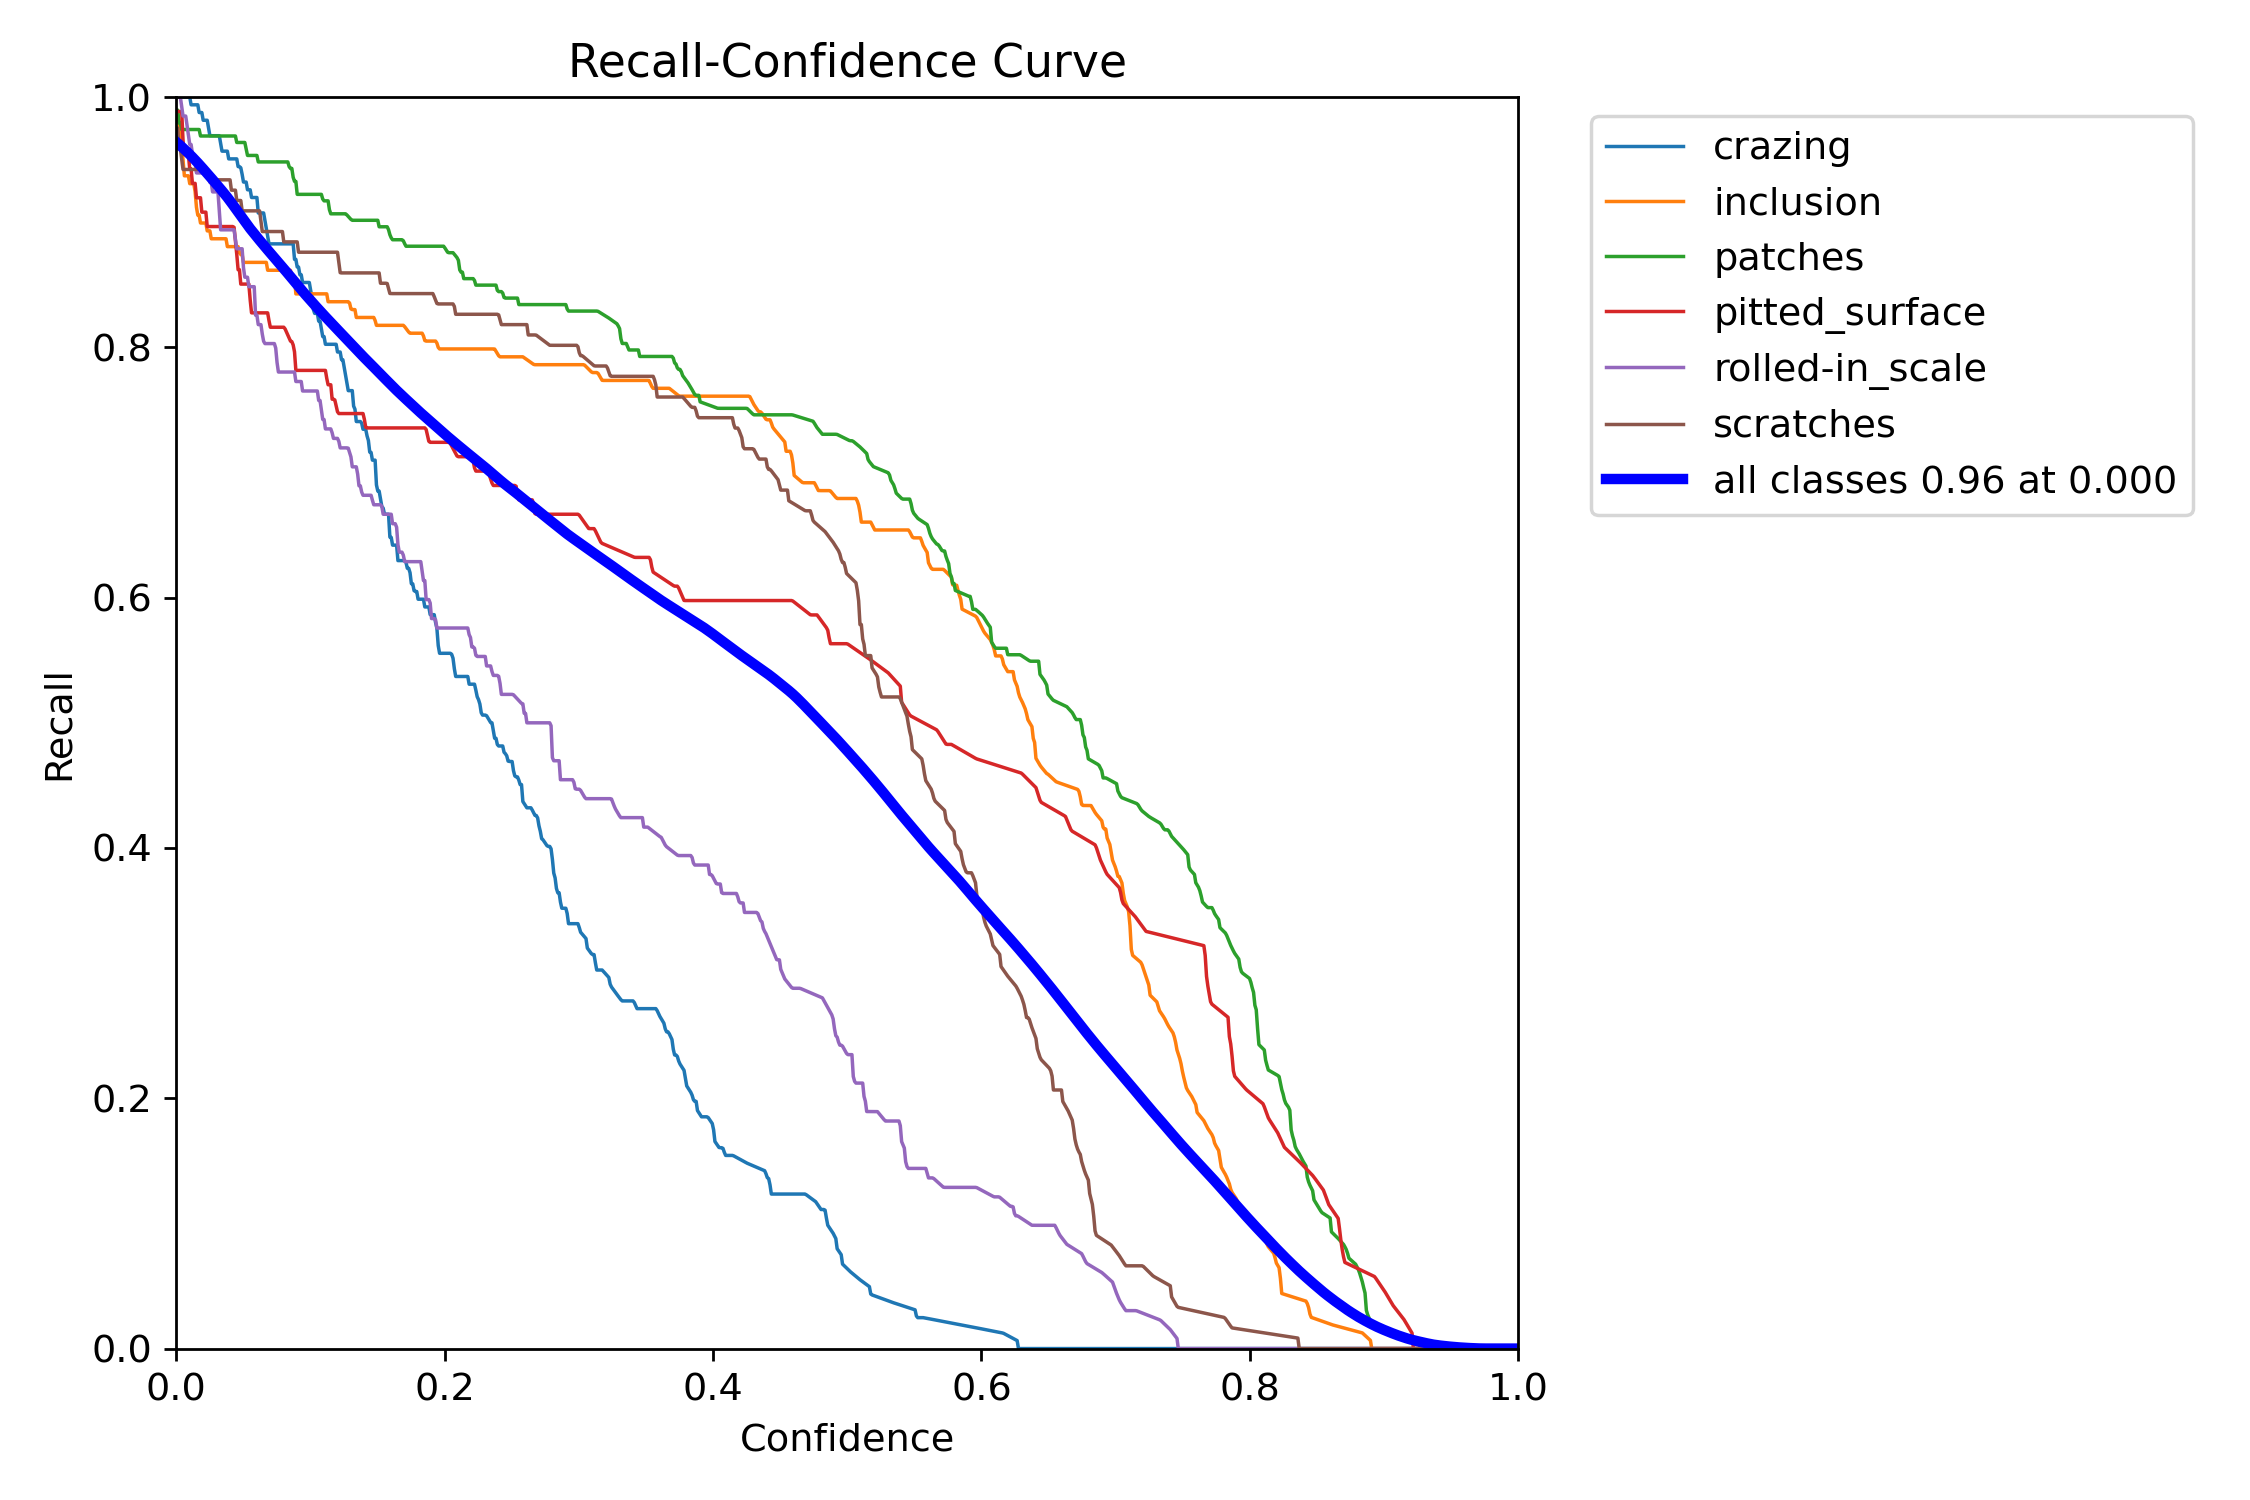
\includegraphics[width=0.46\linewidth]{img/BoxR_curve8n.png}
		
		\vspace{0.25cm}
		
		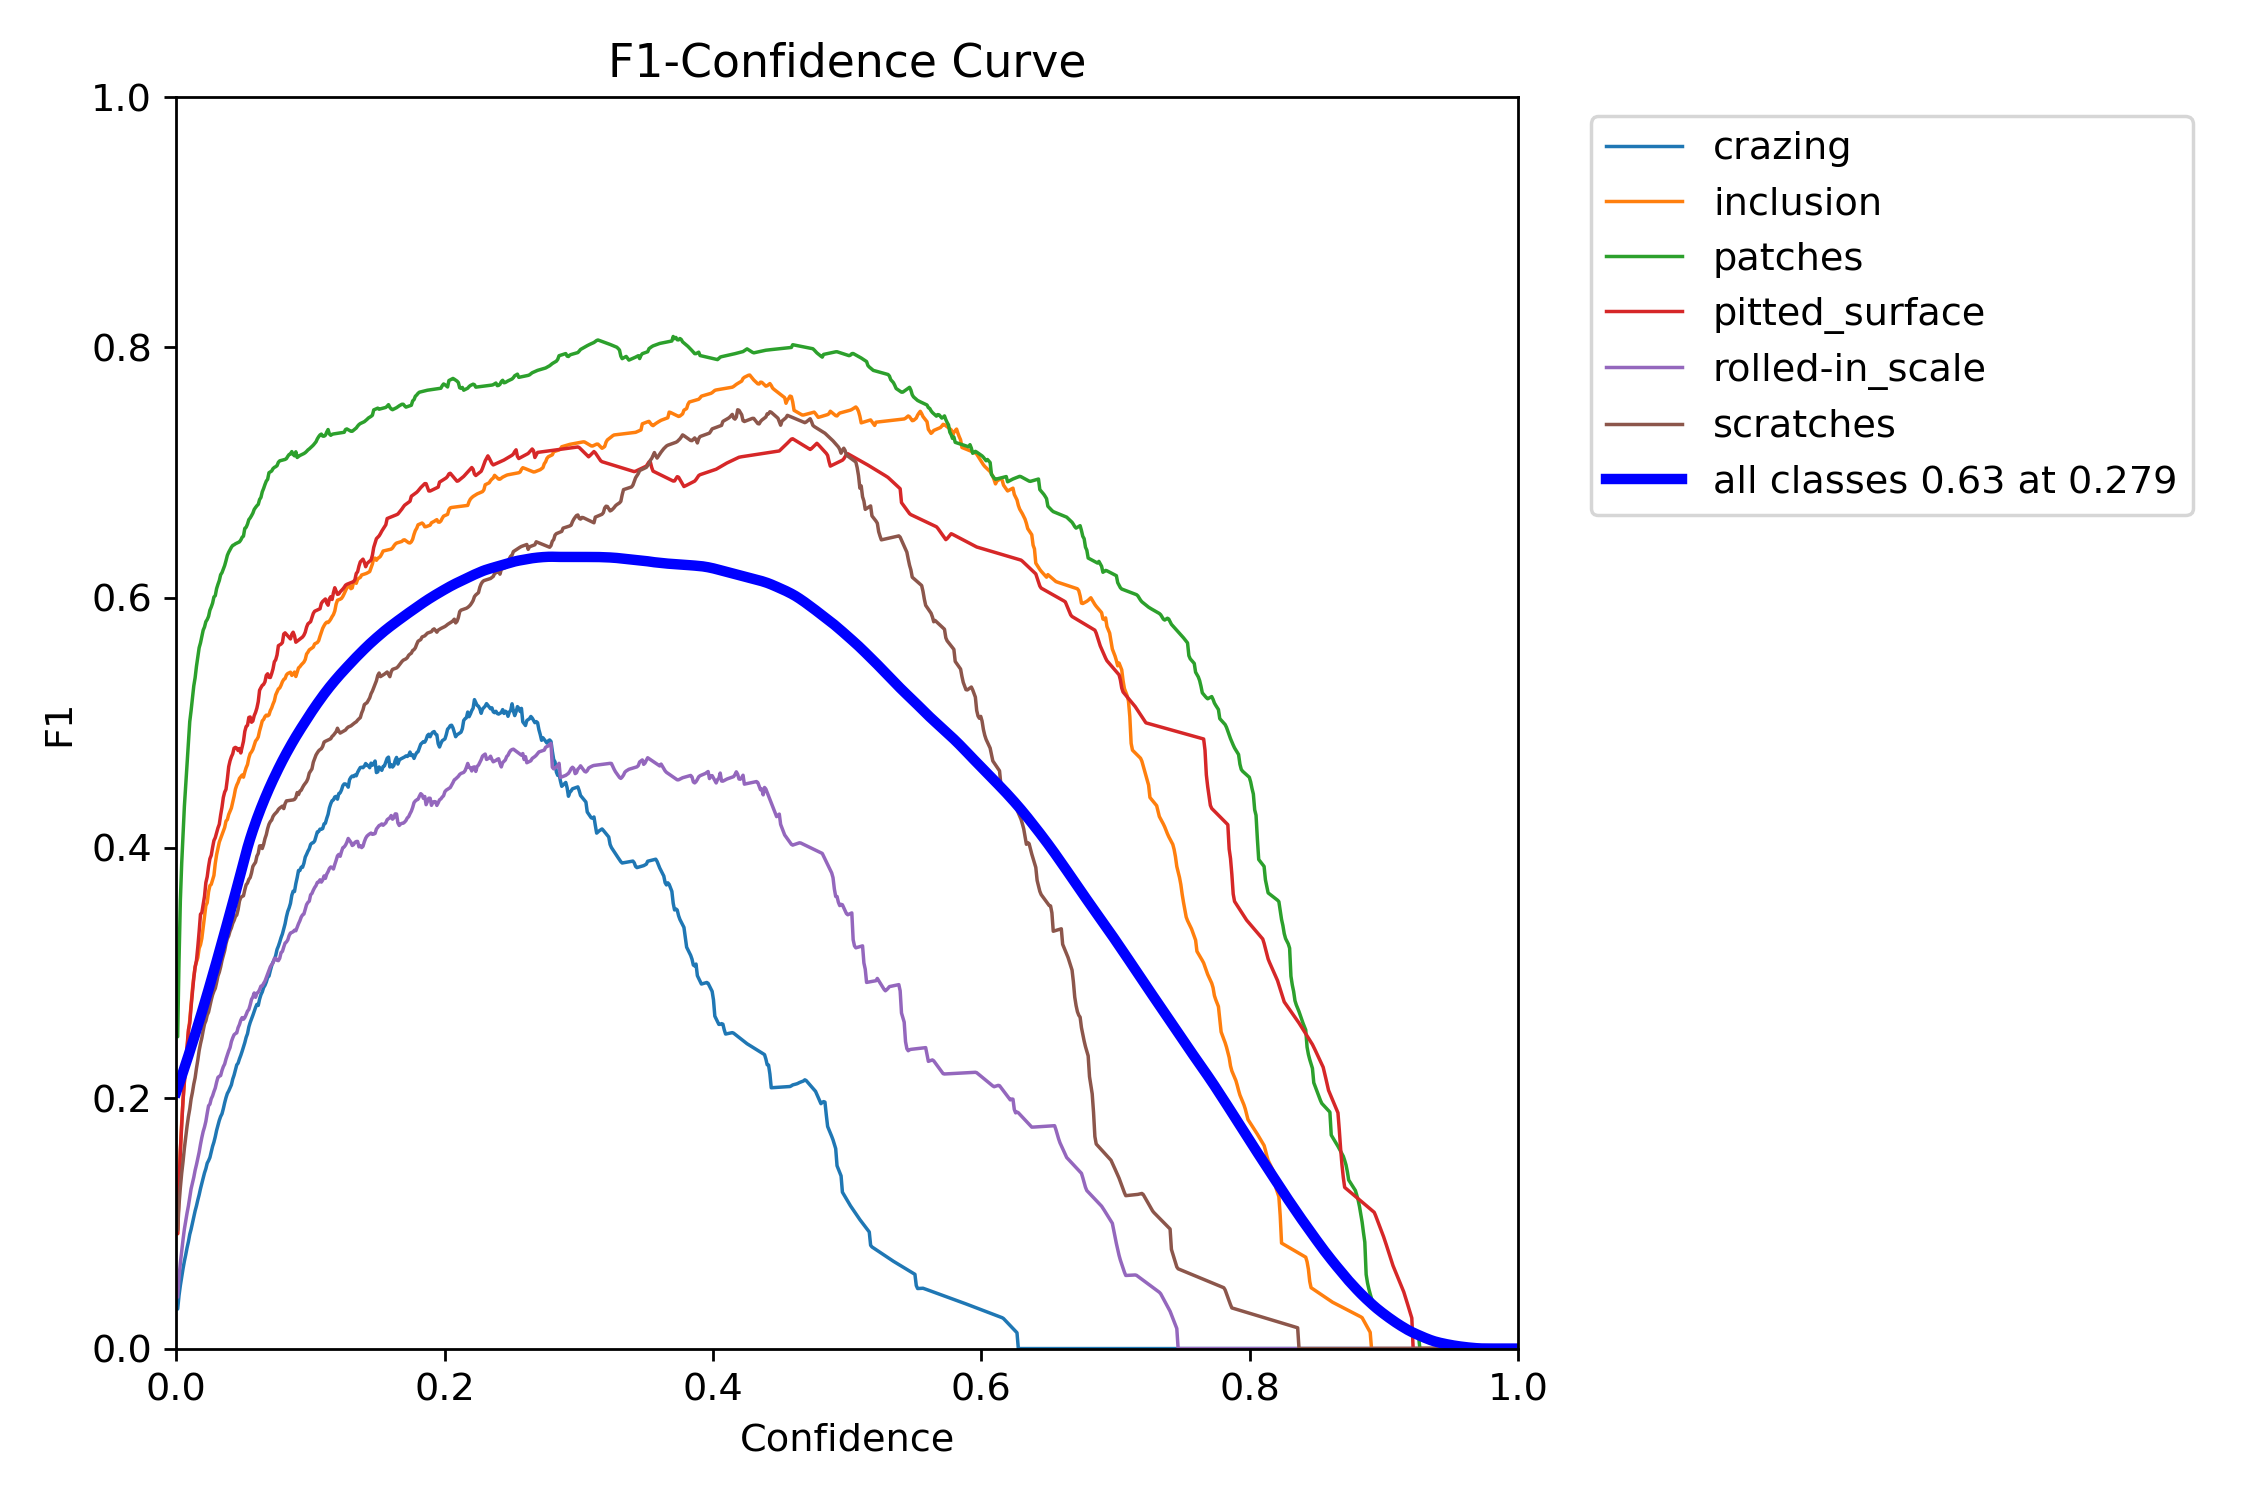
\includegraphics[width=0.46\linewidth]{img/BoxF1_curve8n.png}
		\hfill
		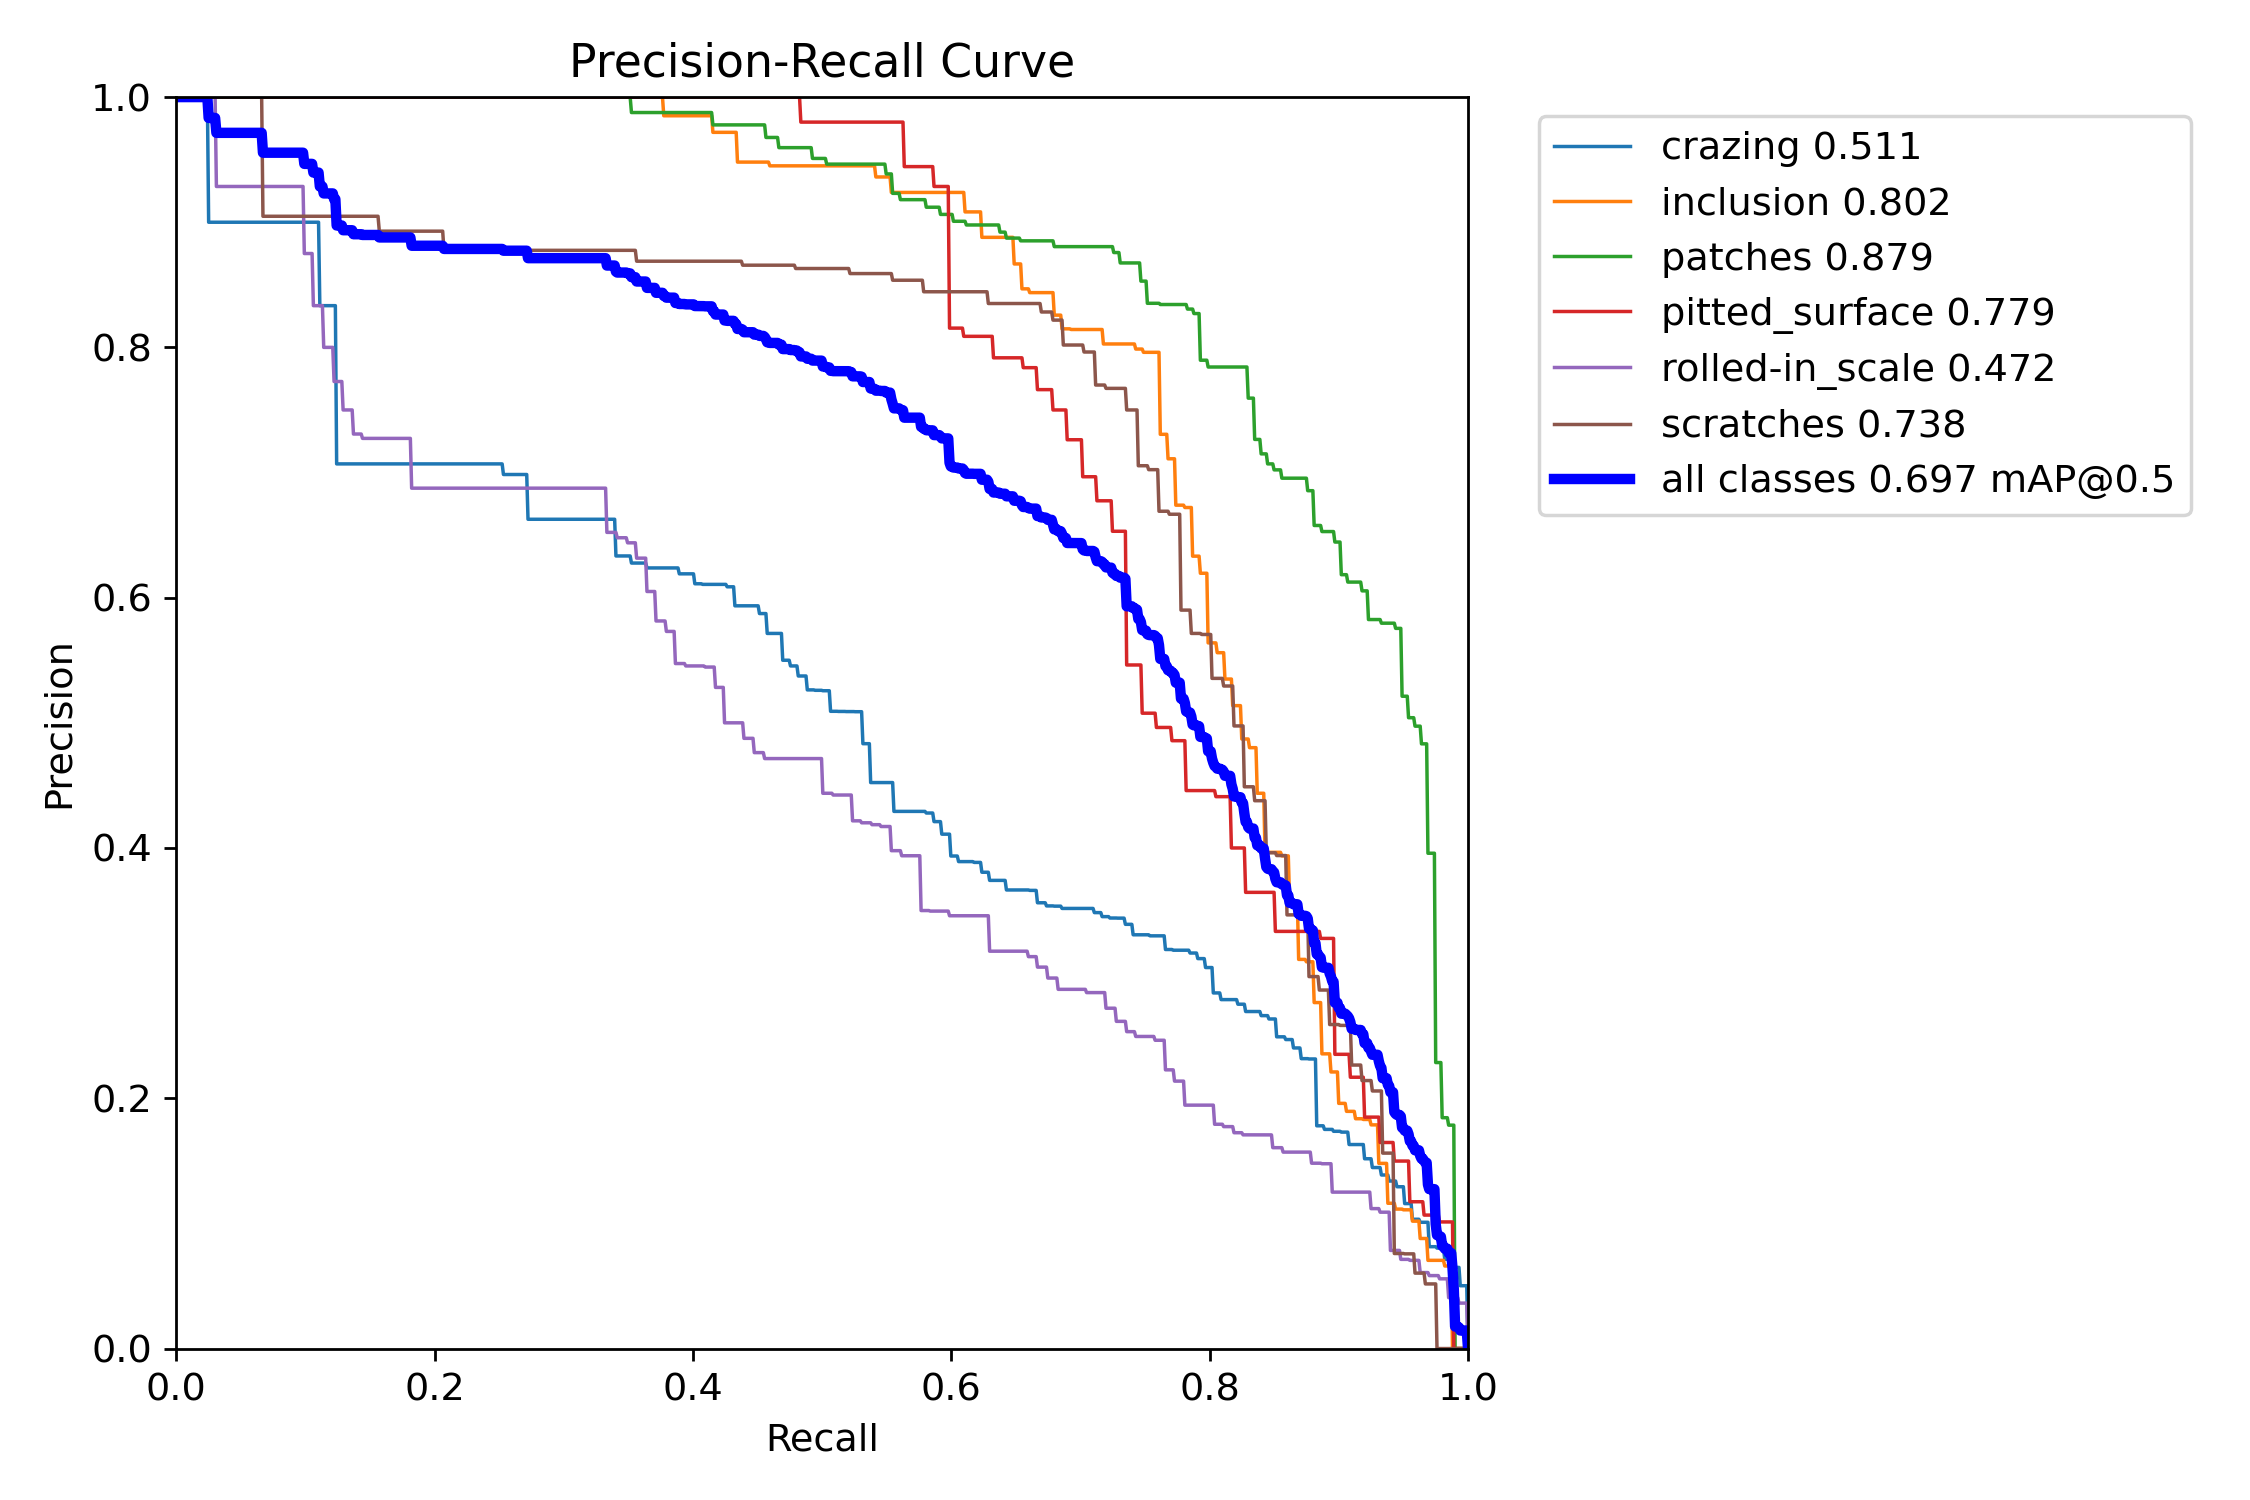
\includegraphics[width=0.46\linewidth]{img/BoxPR_curve8n.png}
		
		\caption{منحنی‌های ارزیابی مدل شامل \lr{Precision}، \lr{Recall}، \lr{F1-score} و \lr{Precision--Recall}}
		\label{fig:box_curves}
	\end{figure}
	
	\paragraph{تحلیل منحنی‌ها}
	با افزایش مقدار \lr{Confidence}، مدل فقط پیش‌بینی‌های مطمئن‌تر را حفظ می‌کند. به همین دلیل، منحنی \lr{Precision} معمولاً روندی افزایشی دارد؛ زیرا با حذف پیش‌بینی‌های کم‌اطمینان، تعداد تشخیص‌های مثبت کاذب کاهش می‌یابد. در مقابل، \lr{Recall} با افزایش آستانه‌ی اطمینان کاهش پیدا می‌کند، زیرا بخشی از عیوبی که با اطمینان کمتری پیش‌بینی شده‌اند حذف می‌شوند. این رفتار نشان‌دهنده‌ی وجود مصالحه‌ی طبیعی میان \lr{Precision} و \lr{Recall} است.
	
	منحنی \lr{F1-score} که میانگین هارمونیک \lr{Precision} و \lr{Recall} است، برای انتخاب آستانه‌ی مناسب اهمیت ویژه‌ای دارد:
	
	\begin{latin}
		\begin{equation}
			F1 = \frac{2PR}{P+R},
		\end{equation}
	\end{latin}
	
	که در آن $P$ و $R$ به‌ترتیب نشان‌دهنده‌ی \lr{Precision} و \lr{Recall} هستند. بیشینه‌ی این منحنی محدوده‌ای را مشخص می‌کند که مدل در آن، تعادل مناسبی میان کاهش تشخیص‌های اشتباه و شناسایی عیوب واقعی برقرار می‌کند. بنابراین، انتخاب آستانه‌ی اطمینان در نزدیکی این ناحیه می‌تواند برای استفاده‌ی عملی از مدل مناسب باشد.
	
	نمودار \lr{Precision--Recall} نیز عملکرد مدل را در آستانه‌های مختلف نشان می‌دهد. قرار گرفتن بخش عمده‌ی منحنی در نواحی بالاتر، بیانگر آن است که مدل توانسته است تعداد قابل قبولی از عیوب واقعی را با میزان مناسبی از تشخیص‌های صحیح شناسایی کند. کاهش تدریجی \lr{Precision} در مقادیر بالاتر \lr{Recall} نشان می‌دهد که شناسایی تعداد بیشتری از عیوب، با افزایش احتمال پیش‌بینی‌های اشتباه همراه می‌شود.
	
	در مجموع، این چهار نمودار نشان می‌دهند که عملکرد مدل به مقدار \lr{Confidence} وابسته است و آستانه‌ی پیش‌فرض الزاماً بهترین انتخاب برای همه‌ی کاربردها نیست. برای بازرسی صنعتی که از دست‌دادن یک عیب اهمیت زیادی دارد، می‌توان آستانه‌ی پایین‌تری انتخاب کرد تا \lr{Recall} افزایش یابد؛ اما اگر کاهش هشدارهای اشتباه اولویت داشته باشد، استفاده از آستانه‌ای بالاتر و نزدیک به بیشینه‌ی \lr{F1-score} مناسب‌تر خواهد بود.
	
	
	ه صورت کلی مدل های سفارشی زده شده که در ادامه ارائه می گردند، عملکرد بهتری دارند اما در برخی از معیارها هم ممکن است مدل \lr{yolov8n} بهتر باشد. تشخیص نادرست بین کلاسی برای پروژه ما به شدت زیان آور است چرا که با پیش بینی اشتباه مدل \lr{Yolov} مقدار ریسک در مراحل بعدی اشتباه محاسبه می شود. این موضوع باعث می شود که عملکرد مدل نهایی در تنظیم سرعت نوار نقاله کاهش یابد.
	
	نمونه ای از نتایج این مدل روی دیتای اعتبارسنجی به صورت زیر است:
	\begin{figure}[H]
		\centering
		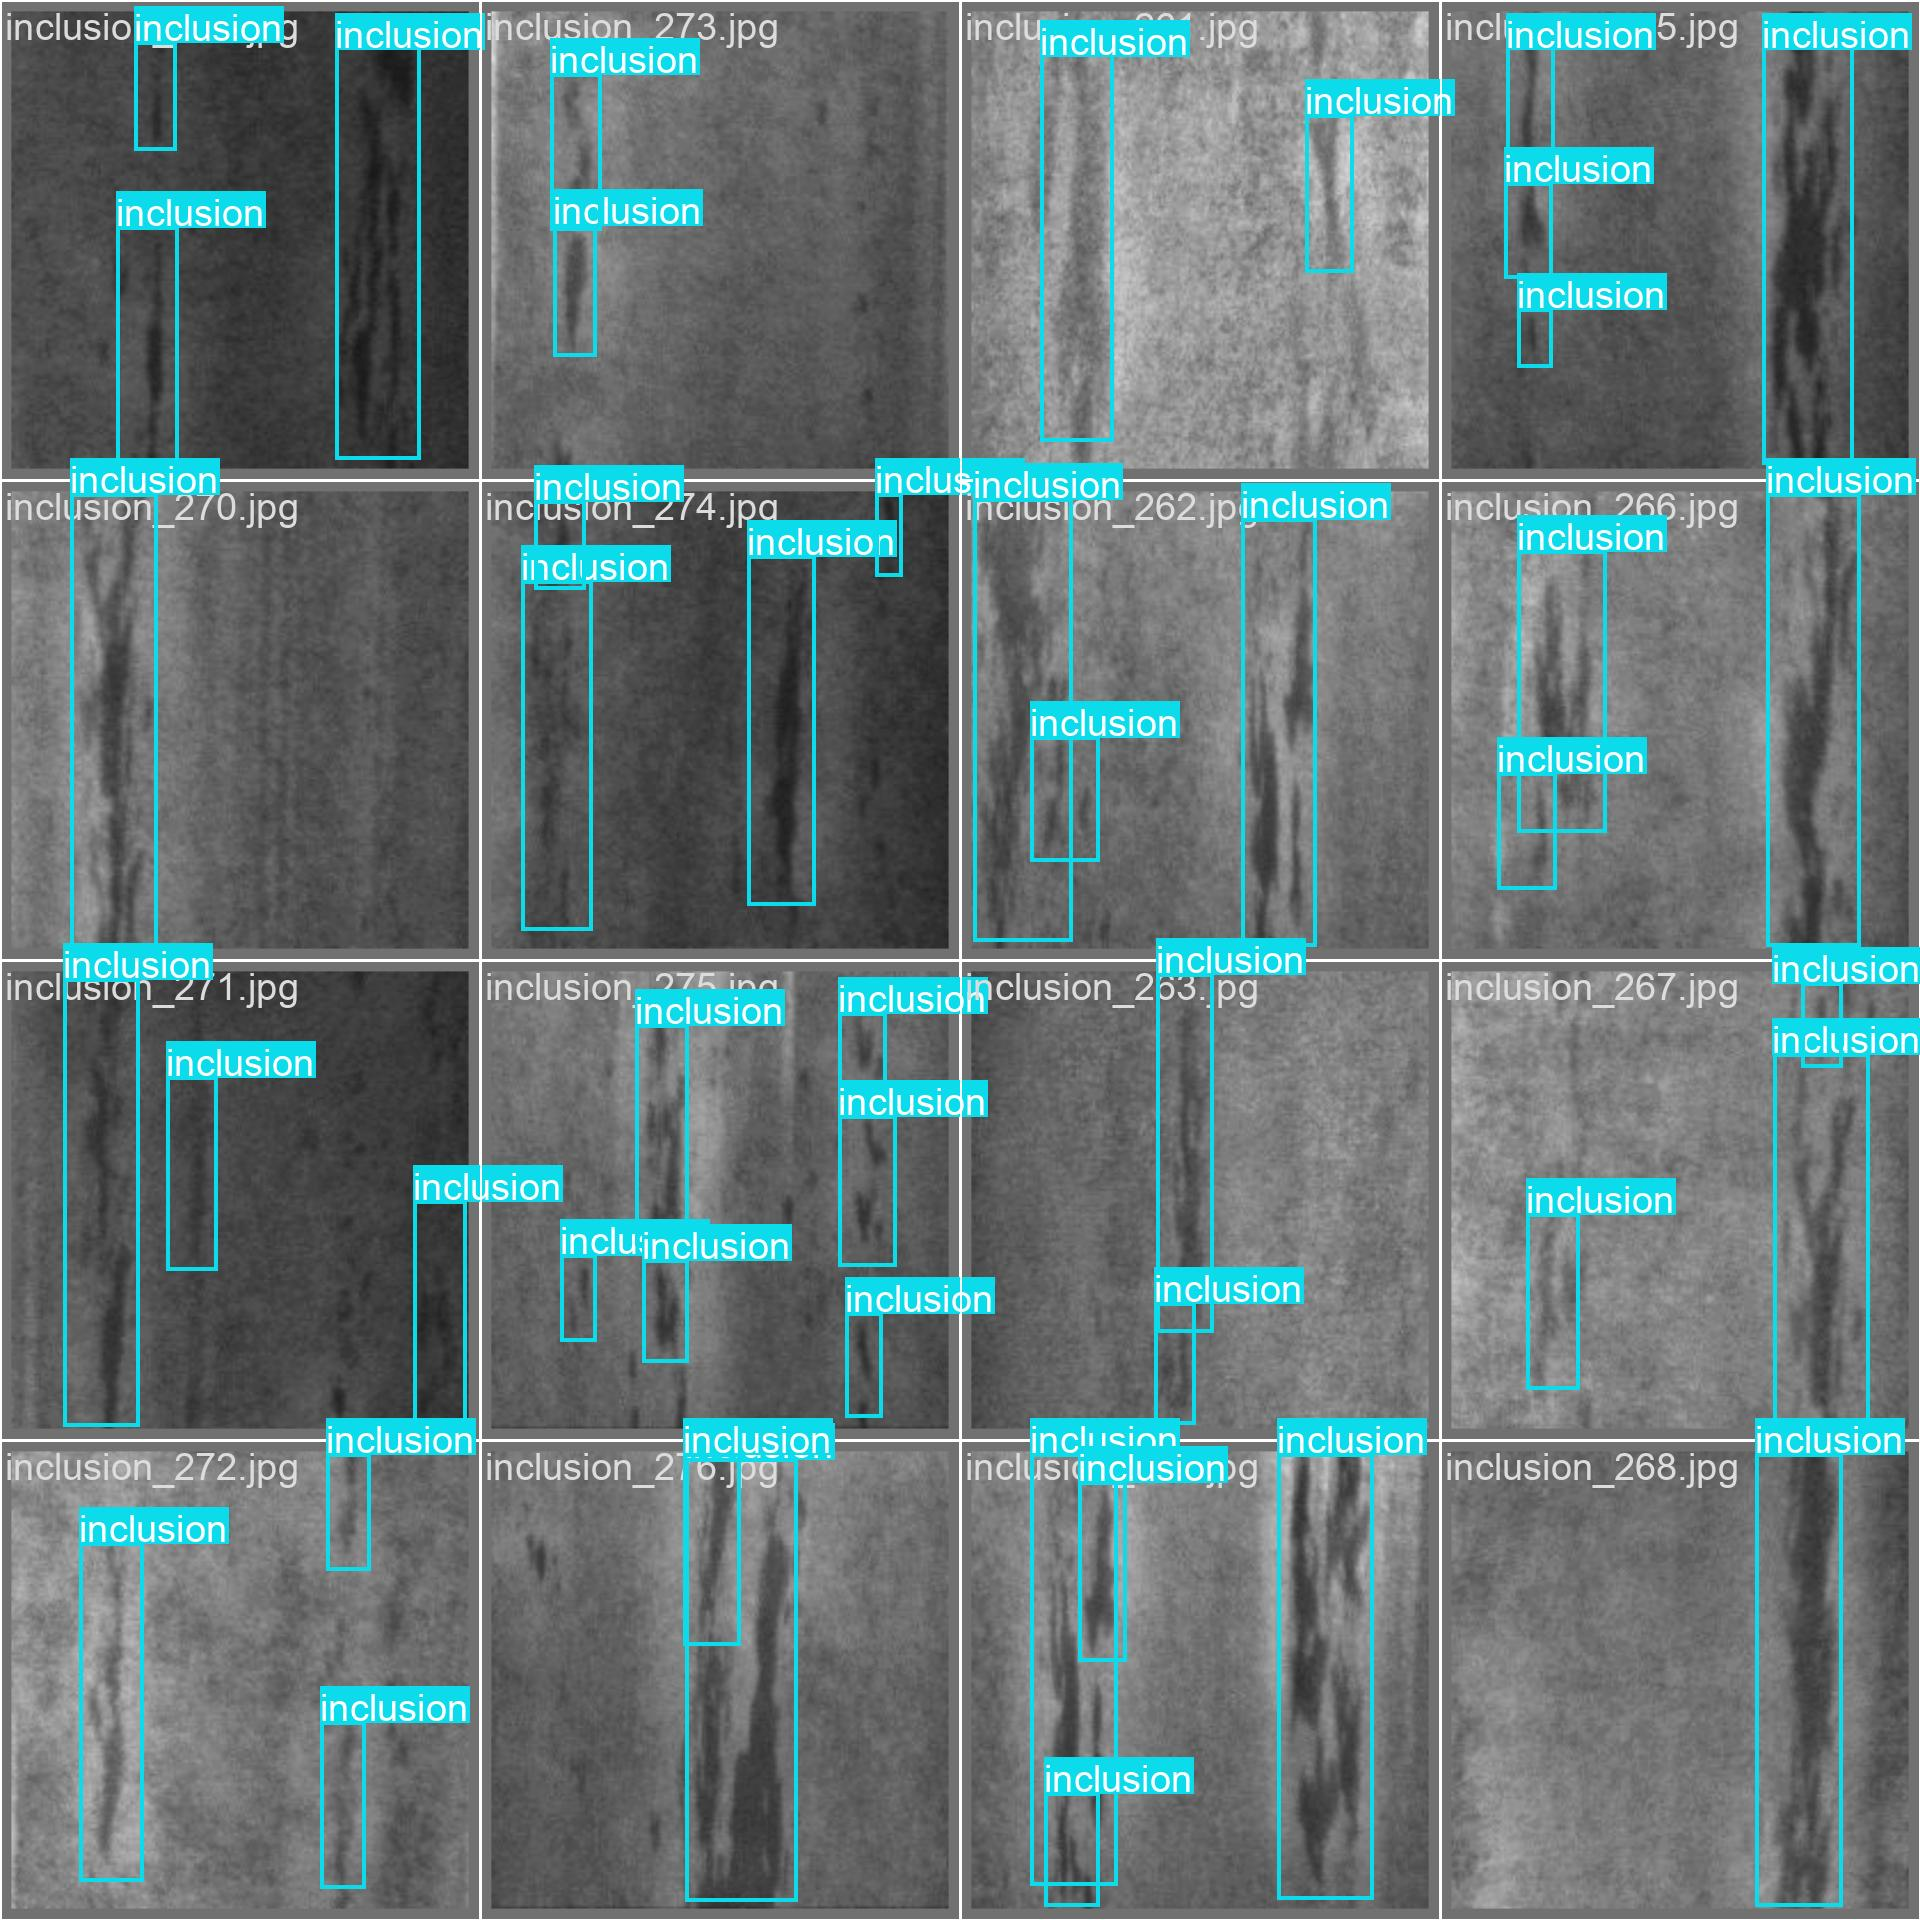
\includegraphics[width=0.2\linewidth]{img/val_batch2_labelsn.jpg}
		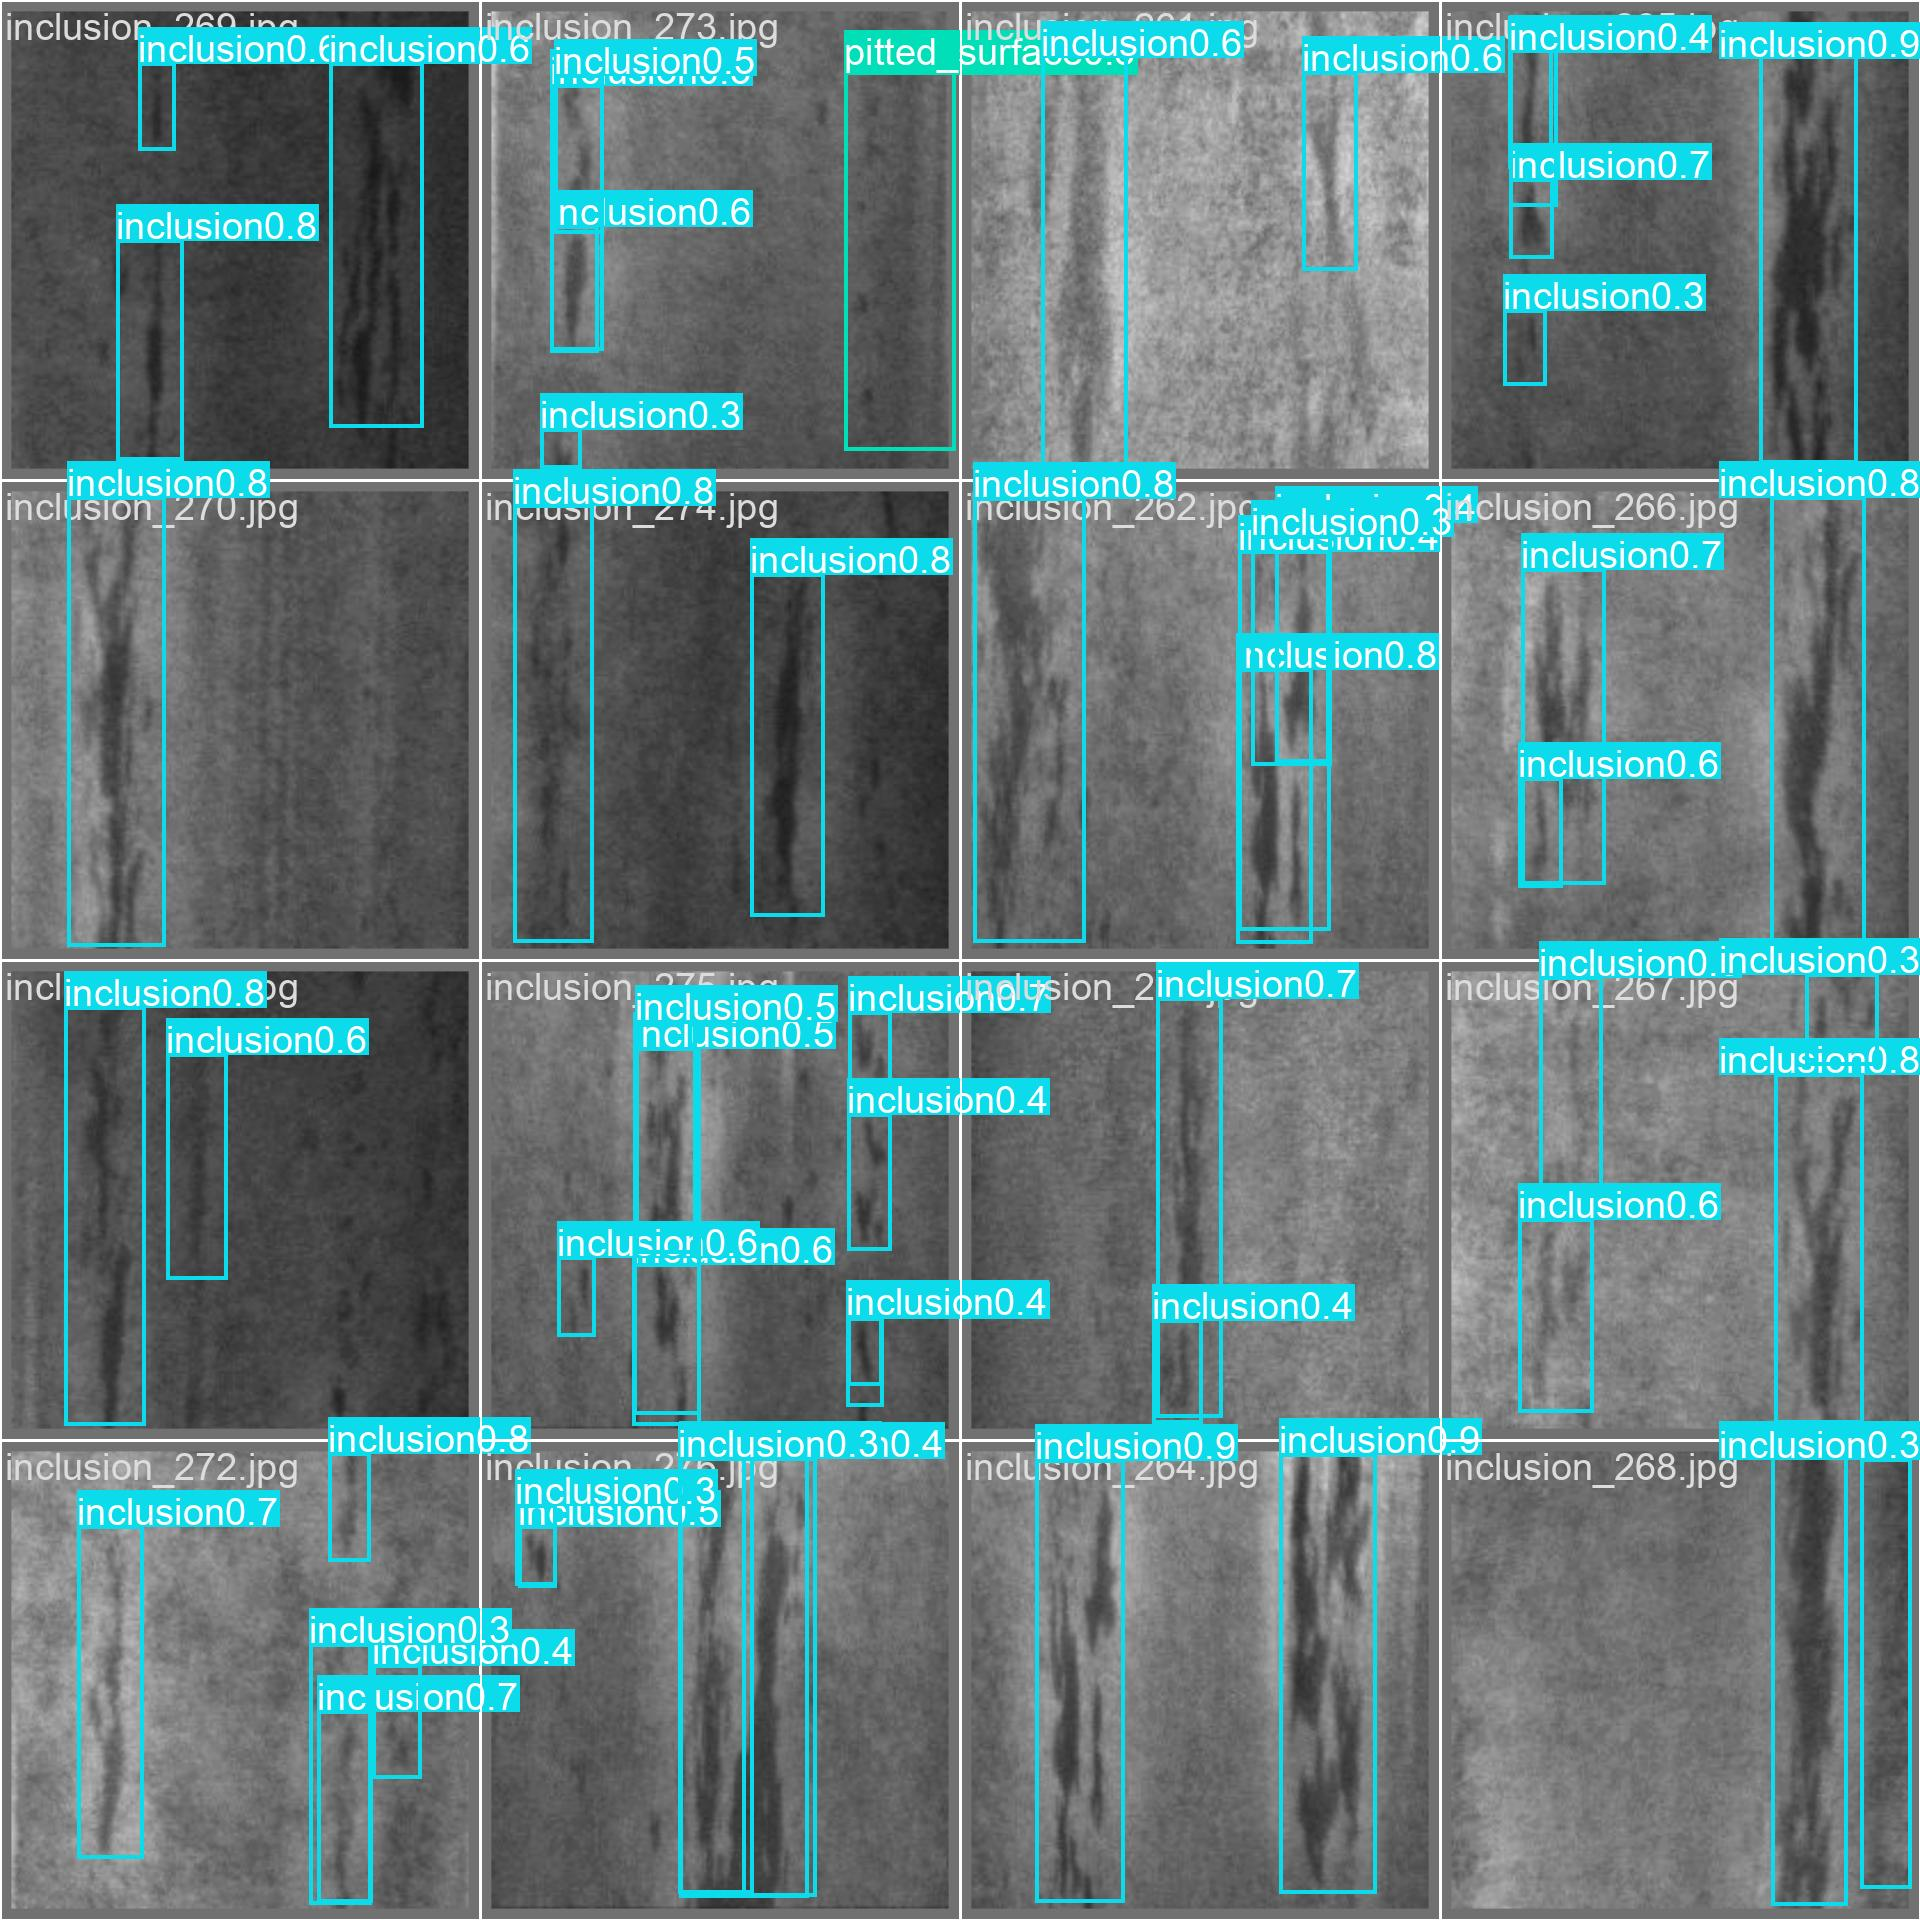
\includegraphics[width=0.2\linewidth]{img/val_batch2_predn.jpg}
		
		\vspace{0.3cm}
		
		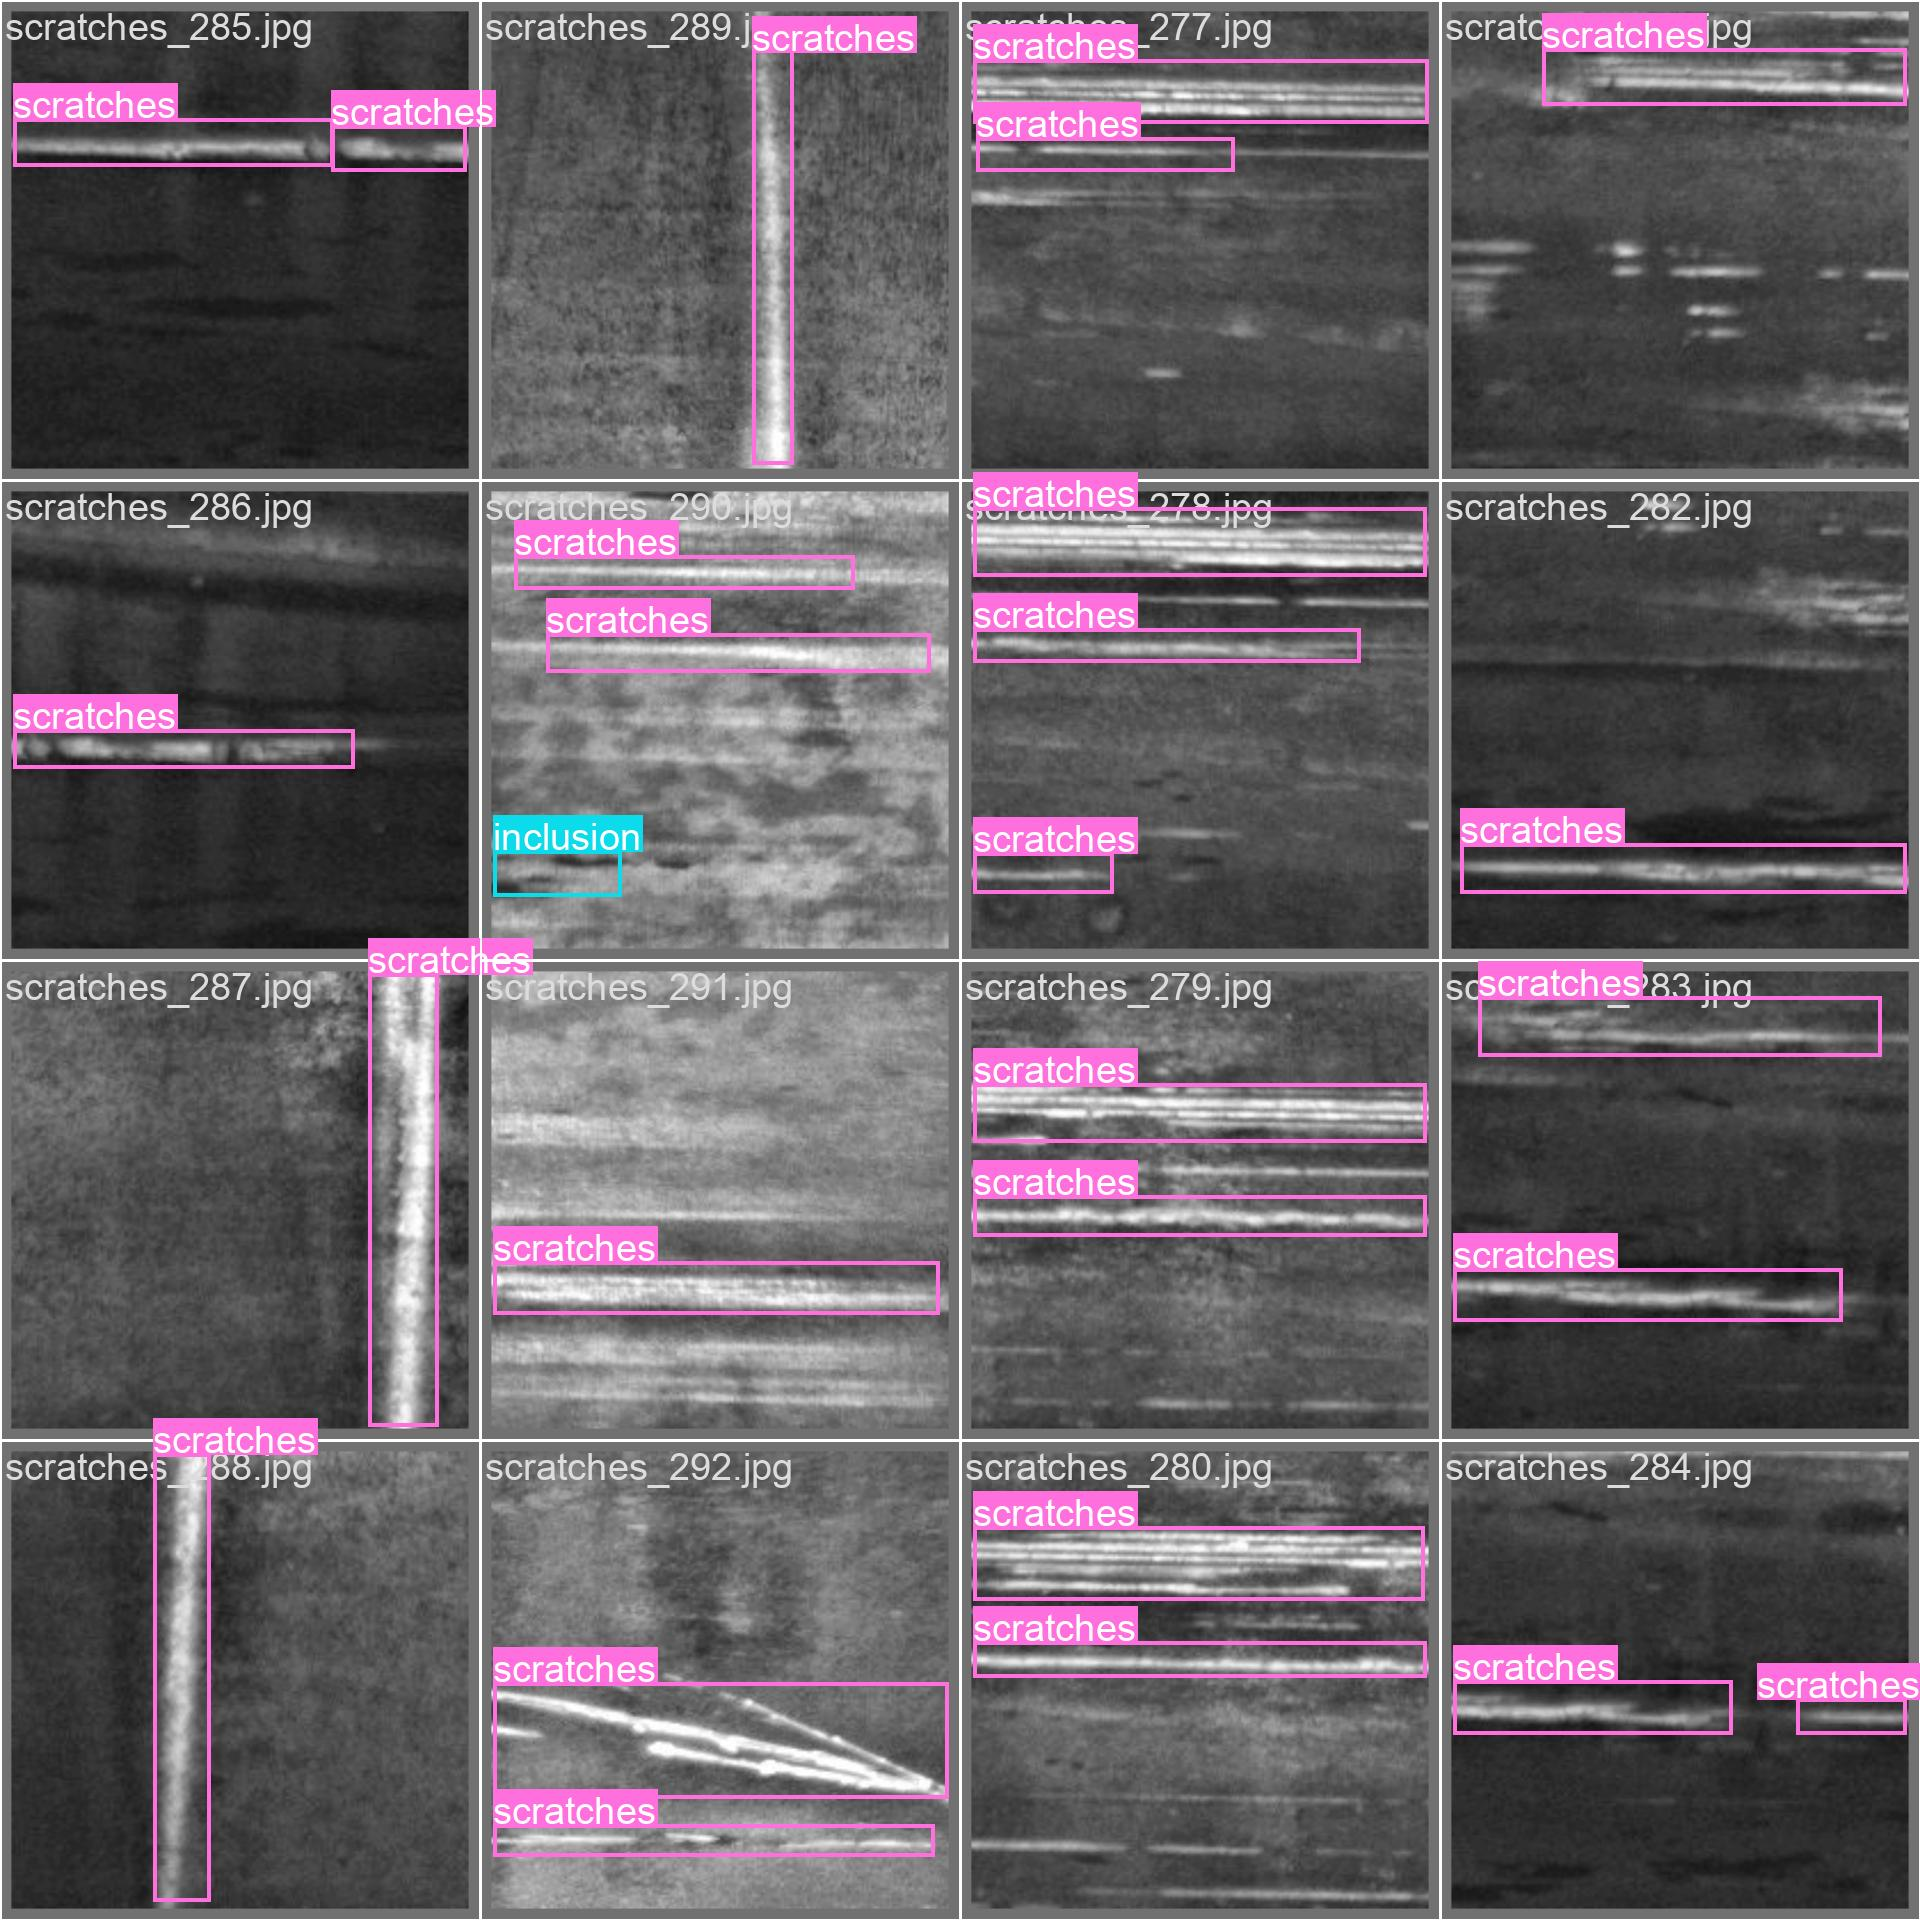
\includegraphics[width=0.2\linewidth]{img/val_batch0_labelsn.jpg}
		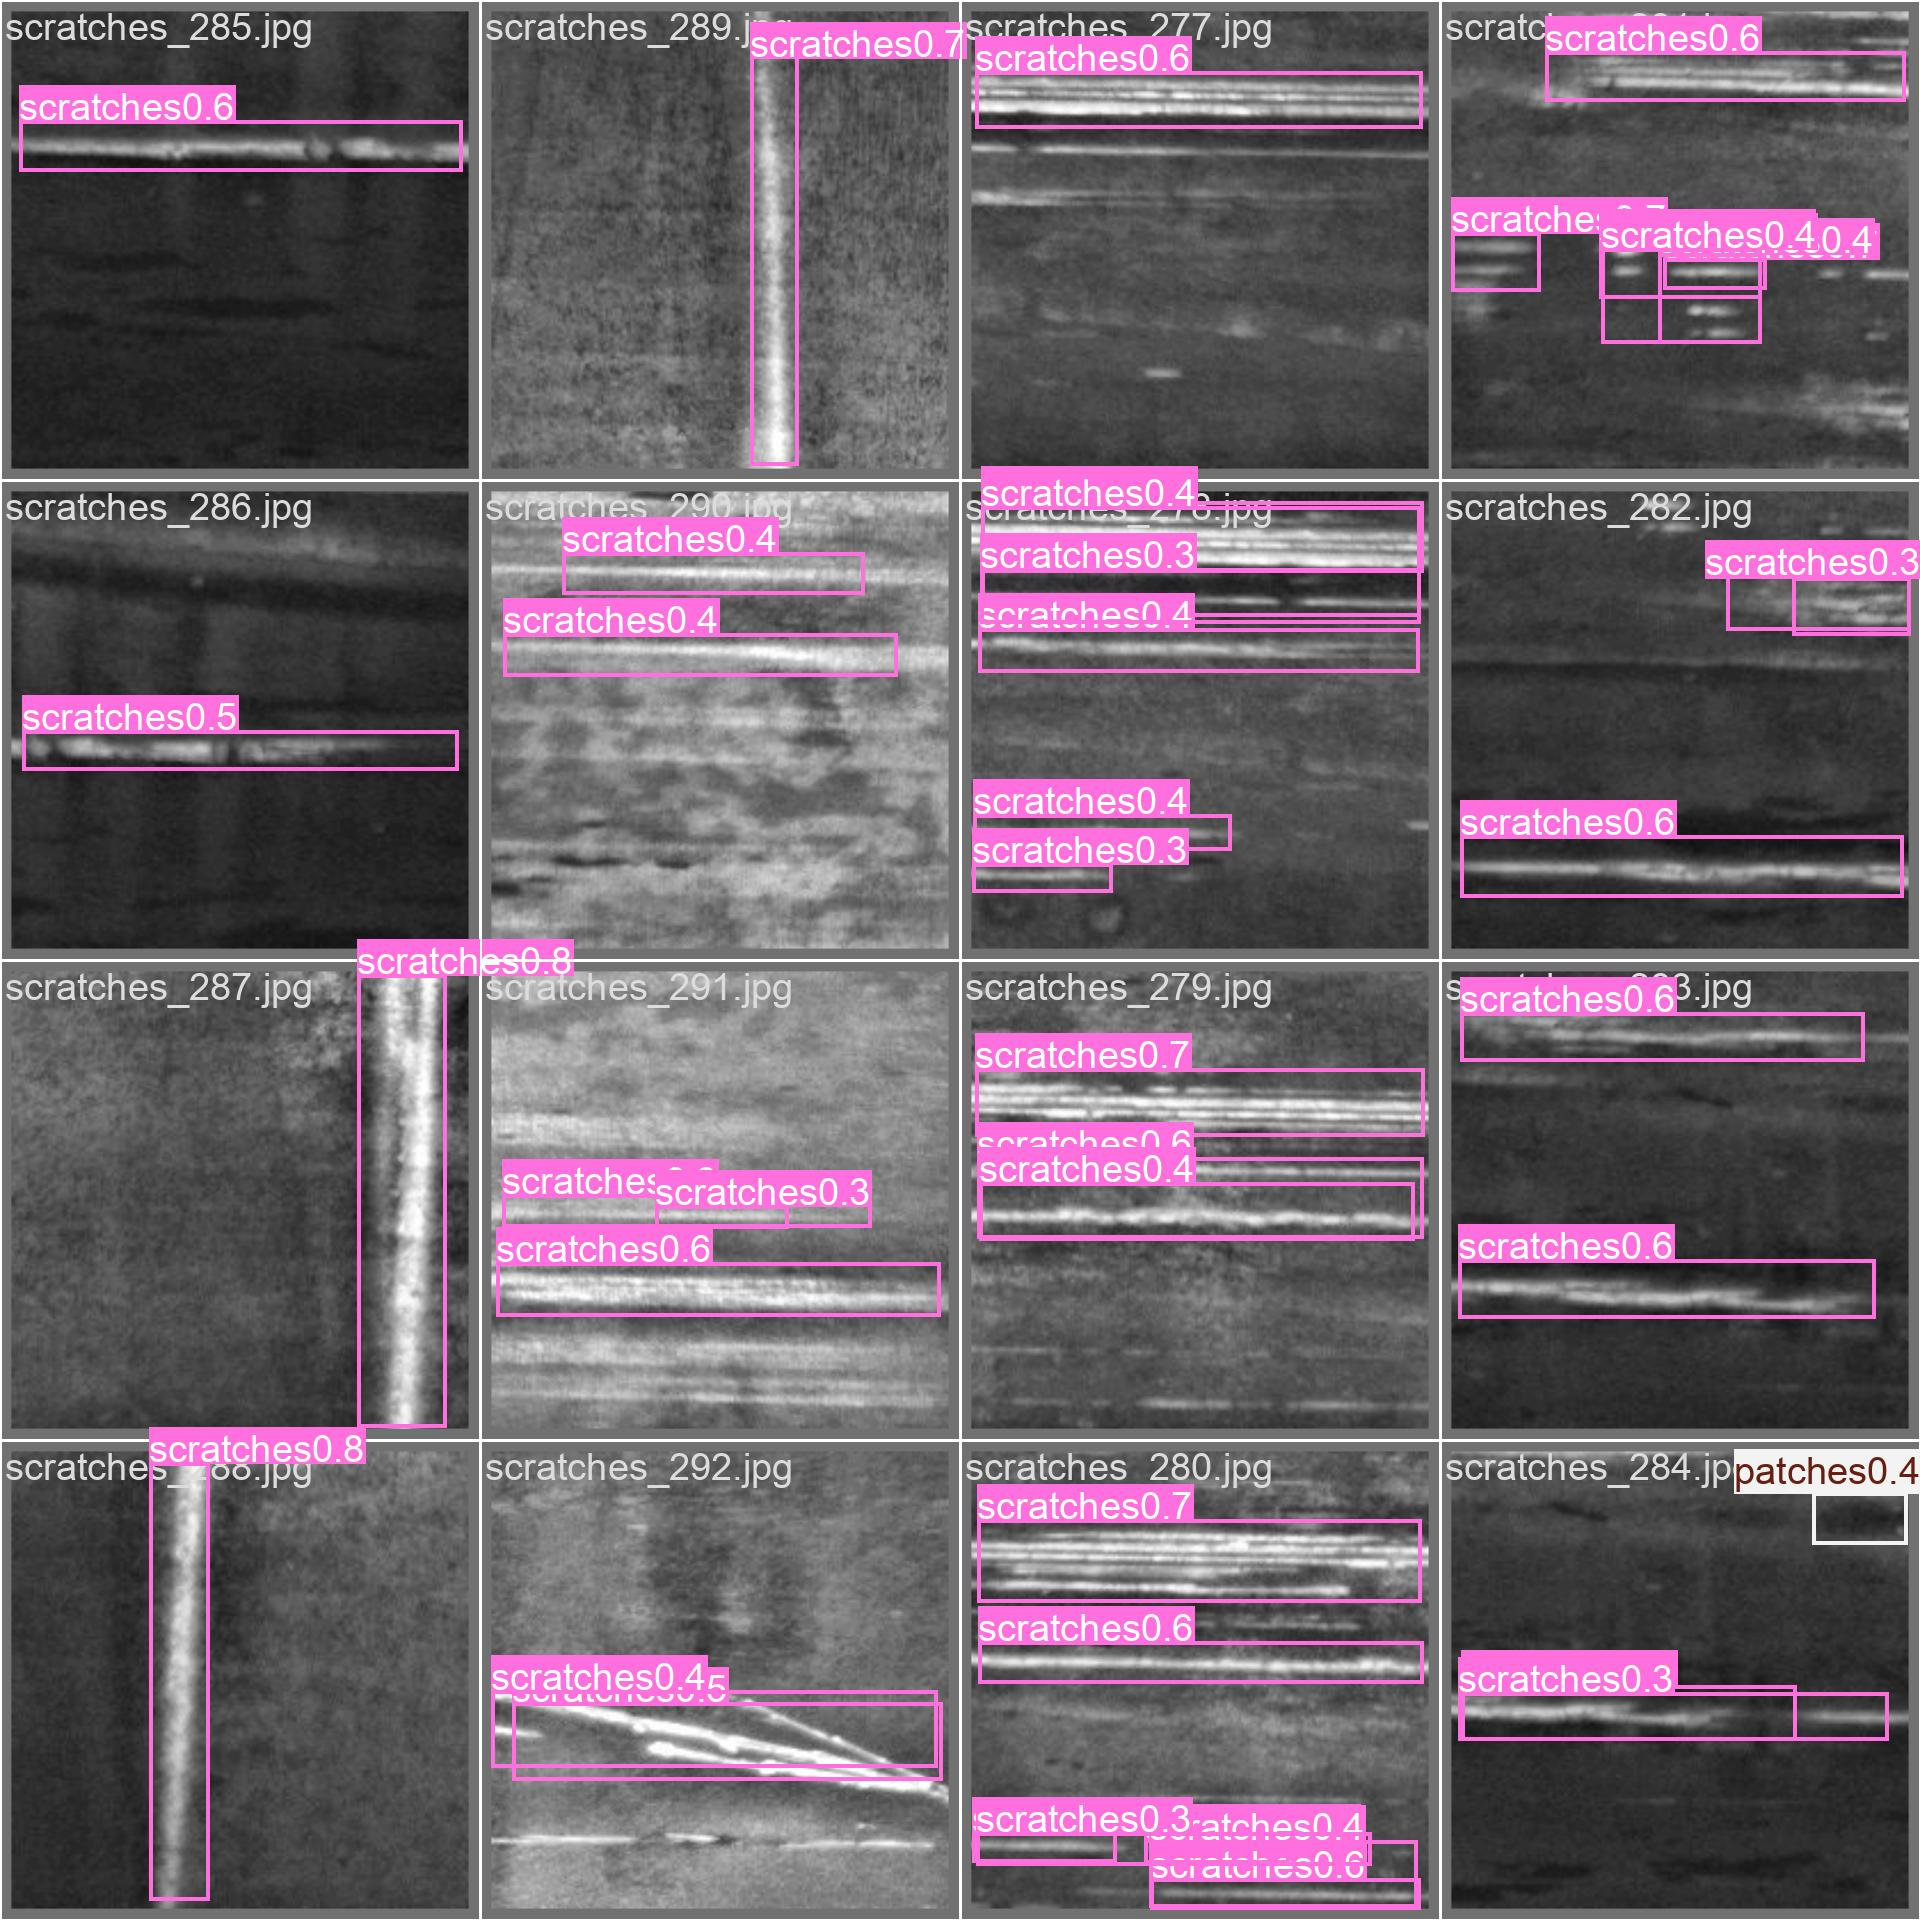
\includegraphics[width=0.2\linewidth]{img/val_batch0_predn.jpg}
		\caption{نمونه‌هایی از تشخیص مدل به همراه \lr{ground truth} آن(تصاویر سمت راست پیش بینی مدل و تصاویر سمت چپ \lr{ground truth})}
	\end{figure}
	
	\newpage
	\subsection{آموزش مدل \lr{YOLOV8-GSEBlock}}
	
	\begin{figure}[H]
		\centering
		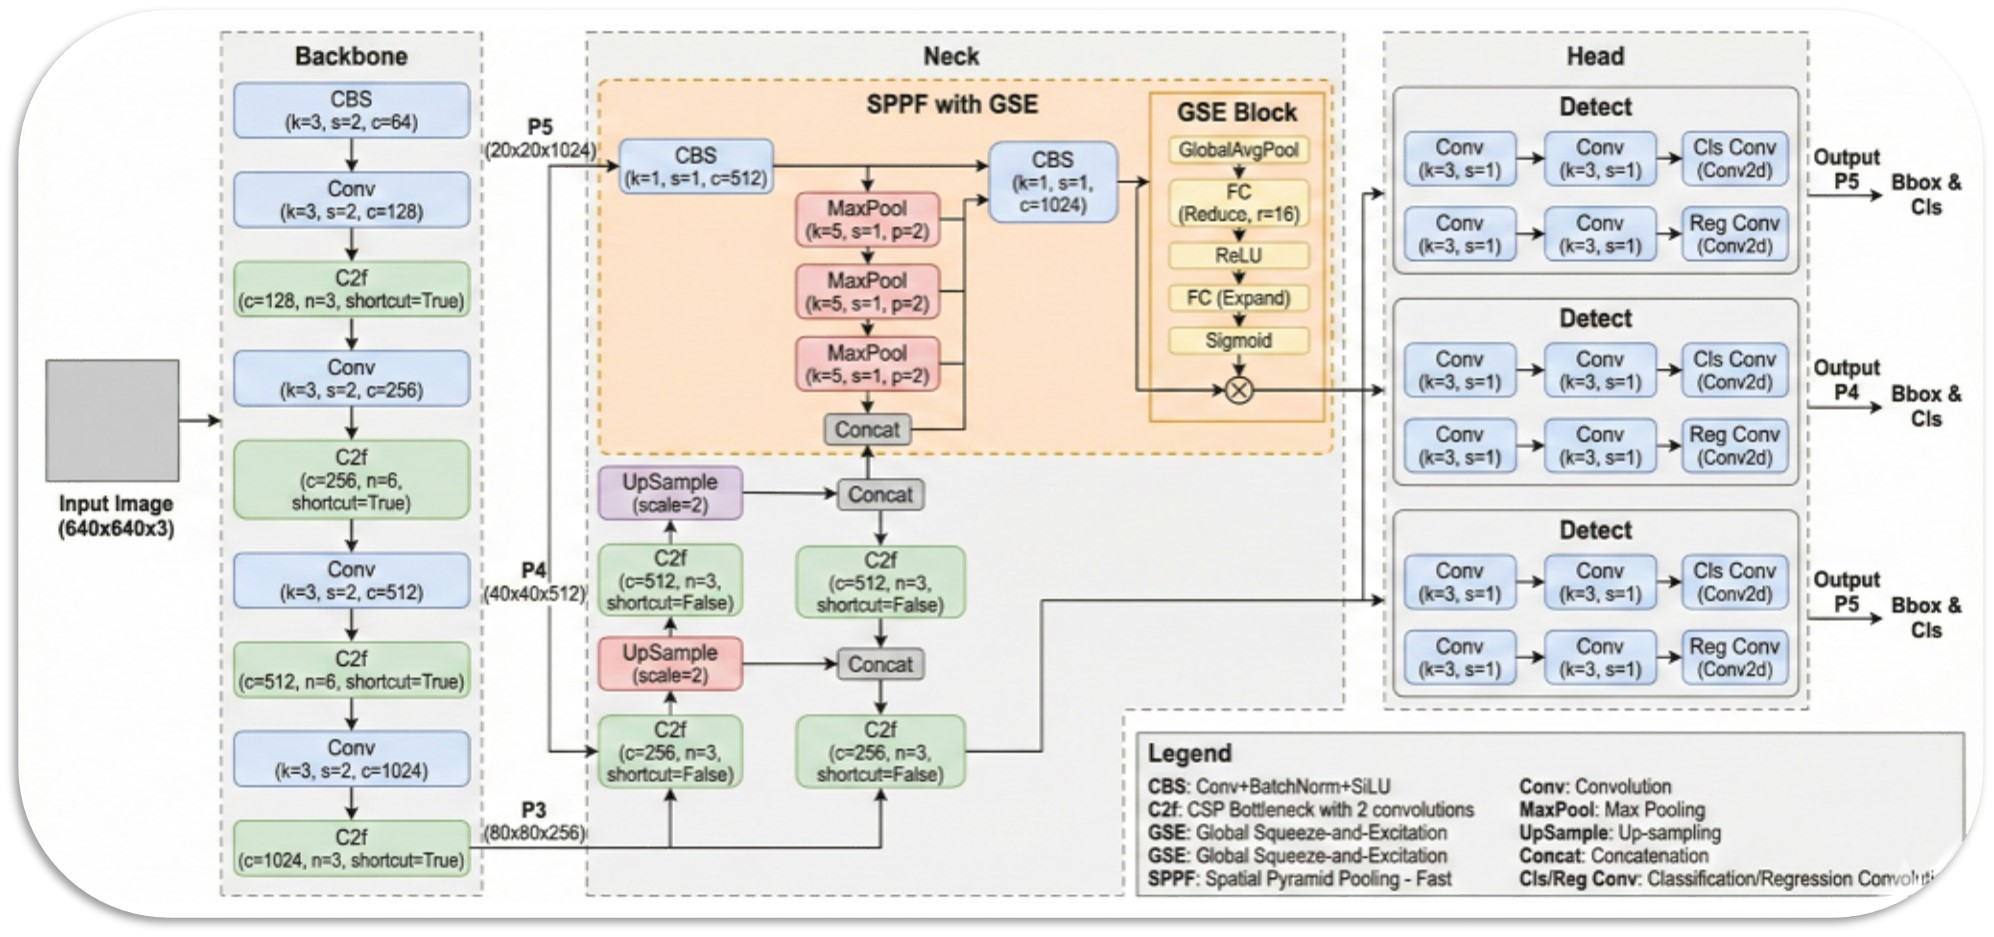
\includegraphics[width=0.8\linewidth]{img/yolov8-gse.jpg}
		\caption{ساختار مدل \lr{yolov8n-gse} (تصویر ساخته شده با هوش مصنوعی)}
	\end{figure}
	
	در این بخش، از مدل YOLOV8 به‌عنوان هسته اصلی تشخیص عیوب سطحی استفاده شده است. YOLOV8 یکی از مدل‌های تک‌مرحله‌ای (\lr{One-Stage Detector}) است که به‌دلیل سرعت بالا و دقت مناسب، گزینه‌ای ایده‌آل برای کاربردهای صنعتی و بلادرنگ محسوب می‌شود. ساختار کلی YOLOV8 شامل سه بخش اصلی است:
	
	\begin{itemize}
		\item \textbf{\lr{Backbone}:} استخراج ویژگی‌های سطح پایین و میانی از تصویر
		\item \textbf{\lr{Neck}:} تجمیع چندمقیاسی ویژگی‌ها (\lr{Feature Fusion})
		\item \textbf{\lr{Head}:} پیش‌بینی کلاس و مختصات جعبه‌های مرزی
	\end{itemize}
	
	در معماری \lr{YOLOV8}، ماژول \lr{SPPF (Spatial Pyramid Pooling - Fast)} در بخش Neck نقش مهمی در افزایش میدان دید مؤثر (\lr{Receptive Field}) و استخراج اطلاعات چندمقیاسی ایفا می‌کند.
	
	\subsection{انگیزه استفاده از ماژول GSE}
	
	عیوب سطحی فولاد معمولاً:
	\begin{itemize}
		\item کوچک و کم‌کنتراست هستند
		\item در بافت‌های پیچیده فلزی پنهان می‌شوند
		\item تفاوت ظریفی با زمینه دارند
	\end{itemize}
	
	در چنین شرایطی، تمام کانال‌های ویژگی استخراج‌شده اهمیت یکسانی ندارند. برخی کانال‌ها حاوی اطلاعات حیاتی مرتبط با خرابی هستند، در حالی که سایر کانال‌ها عمدتاً نویز یا بافت زمینه را نمایش می‌دهند.  
	
	به‌منظور تقویت کانال‌های مهم و تضعیف کانال‌های غیرمؤثر، از یک ماژول توجه کانالی بهبودیافته تحت عنوان \lr{GSE (Global Squeeze Enhancement)} استفاده شده است.
	
	\subsection{ساختار ماژول GSE بهبودیافته}
	
	ماژول GSE پیشنهادی از ترکیب همزمان اطلاعات آماری میانگین و بیشینه کانال‌ها استفاده می‌کند. ساختار این ماژول شامل مراحل زیر است:
	
	\subsubsection{فشرده‌سازی سراسری (\lr{Global Squeeze})}
	
	ابتدا دو نوع pooling سراسری بر روی نقشه ویژگی ورودی \(X \in \mathbb{R}^{C \times H \times W}\) اعمال می‌شود:
	
	\[
	\text{GAP}(X) = \frac{1}{H \times W} \sum_{i=1}^{H} \sum_{j=1}^{W} X_{c,i,j}
	\]
	
	\[
	\text{GMP}(X) = \max_{i,j}(X_{c,i,j})
	\]
	
	که به‌ترتیب نمایانگر میانگین و بیشینه اطلاعات هر کانال هستند. ترکیب این دو دیدگاه باعث می‌شود هم اطلاعات کلی و هم ویژگی‌های برجسته حفظ شوند.
	
	\subsubsection{یادگیری وزن‌های کانالی}
	
	خروجی‌های pooling با یکدیگر جمع شده و وارد یک شبکه کوچک کانولوشنی شامل دو لایه \(1 \times 1\) می‌شوند:
	
	\[
	S = \sigma(W_2 \cdot \delta(W_1 \cdot (GAP + GMP)))
	\]
	
	که در آن:
	\begin{itemize}
		\item \(W_1\) و \(W_2\): وزن‌های کانولوشنی
		\item \(\delta\): تابع فعال‌ساز ReLU
		\item \(\sigma\): تابع سیگموید
	\end{itemize}
	
	خروجی \(S\) یک بردار وزن کانالی در بازه \([0,1]\) است.
	
	\subsubsection{بازکالیبراسیون ویژگی‌ها}
	
	در نهایت، نقشه ویژگی ورودی در وزن‌های کانالی ضرب می‌شود:
	
	\[
	X' = X \odot S
	\]
	
	این عملیات موجب تقویت کانال‌های مرتبط با عیوب سطحی و تضعیف کانال‌های غیرضروری می‌شود.
	
	\subsection{ادغام ماژول GSE با SPPF در YOLOV8}
	
	در این پروژه، ماژول GSE به‌صورت هوشمندانه پس از خروجی ماژول SPPF در بخش Neck مدل YOLOV8 افزوده شده است. دلیل این انتخاب آن است که خروجی SPPF شامل ویژگی‌های چندمقیاسی و غنی‌شده است و اعمال توجه کانالی در این مرحله بیشترین تأثیر را بر کیفیت ویژگی‌های منتقل‌شده به Head خواهد داشت.
	
	به‌منظور حفظ سازگاری با معماری اصلی و جلوگیری از تغییرات گسترده، تابع forward ماژول SPPF به‌صورت پویا بازنویسی شده و ماژول GSE تنها یک‌بار در زمان اجرا ایجاد می‌شود. این رویکرد:
	\begin{itemize}
		\item سربار محاسباتی ناچیزی ایجاد می‌کند
		\item امکان استفاده از وزن‌های از پیش آموزش‌دیده YOLOV8 را حفظ می‌کند
		\item به‌سادگی قابل تعمیم به نسخه‌های دیگر YOLOv است
	\end{itemize}
	
	\subsection{استراتژی آموزش مدل}
	
	آموزش مدل با استفاده از وزن‌های از پیش آموزش‌دیده YOLOV8n آغاز شده است که موجب تسریع همگرایی و کاهش نیاز به داده‌های بسیار زیاد می‌شود. تنظیمات آموزش به شرح زیر است:
	
	\begin{itemize}
		\item \textbf{\lr{Optimizer}:} AdamW (به‌منظور کنترل بهتر \lr{overfitting})
		\item \textbf{\lr{Learning Rate} اولیه:} \(10^{-3}\)
		\item \textbf{\lr{Scheduler}:} \lr{Cosine Annealing}
		\item \textbf{\lr{Warm-up}:} ۵ \lr{epoch}
		\item \textbf{\lr{Batch Size}:} ۱۶
		\item \textbf{\lr{Image Size}:} \(640 \times 640\)
		\item \textbf{\lr{Epochs}:} ۳۰۰
	\end{itemize}
	
	برای جلوگیری از یادگیری الگوهای غیرواقعی، تکنیک‌های افزایش داده شدید نظیر Mosaic، MixUp و CutMix غیرفعال شده‌اند و تنها تبدیلات هندسی ملایم مانند چرخش، مقیاس‌دهی و وارونگی اعمال شده است. این انتخاب با هدف حفظ ماهیت صنعتی داده‌ها انجام شده است.
	
	\subsection{کنترل بیش‌برازش و توقف زودهنگام}
	
	به‌منظور جلوگیری از بیش‌برازش، از مکانیزم \lr{Early Stopping} با مقدار \lr{patience} برابر با ۵۰ استفاده شده است. بدین معنا که در صورت عدم بهبود معیارهای اعتبارسنجی، فرآیند آموزش به‌صورت خودکار متوقف می‌شود.
	
	نتایج آموزش این مدل به صورت زیر می‌باشد:
	\begin{figure}[H]
		\centering
		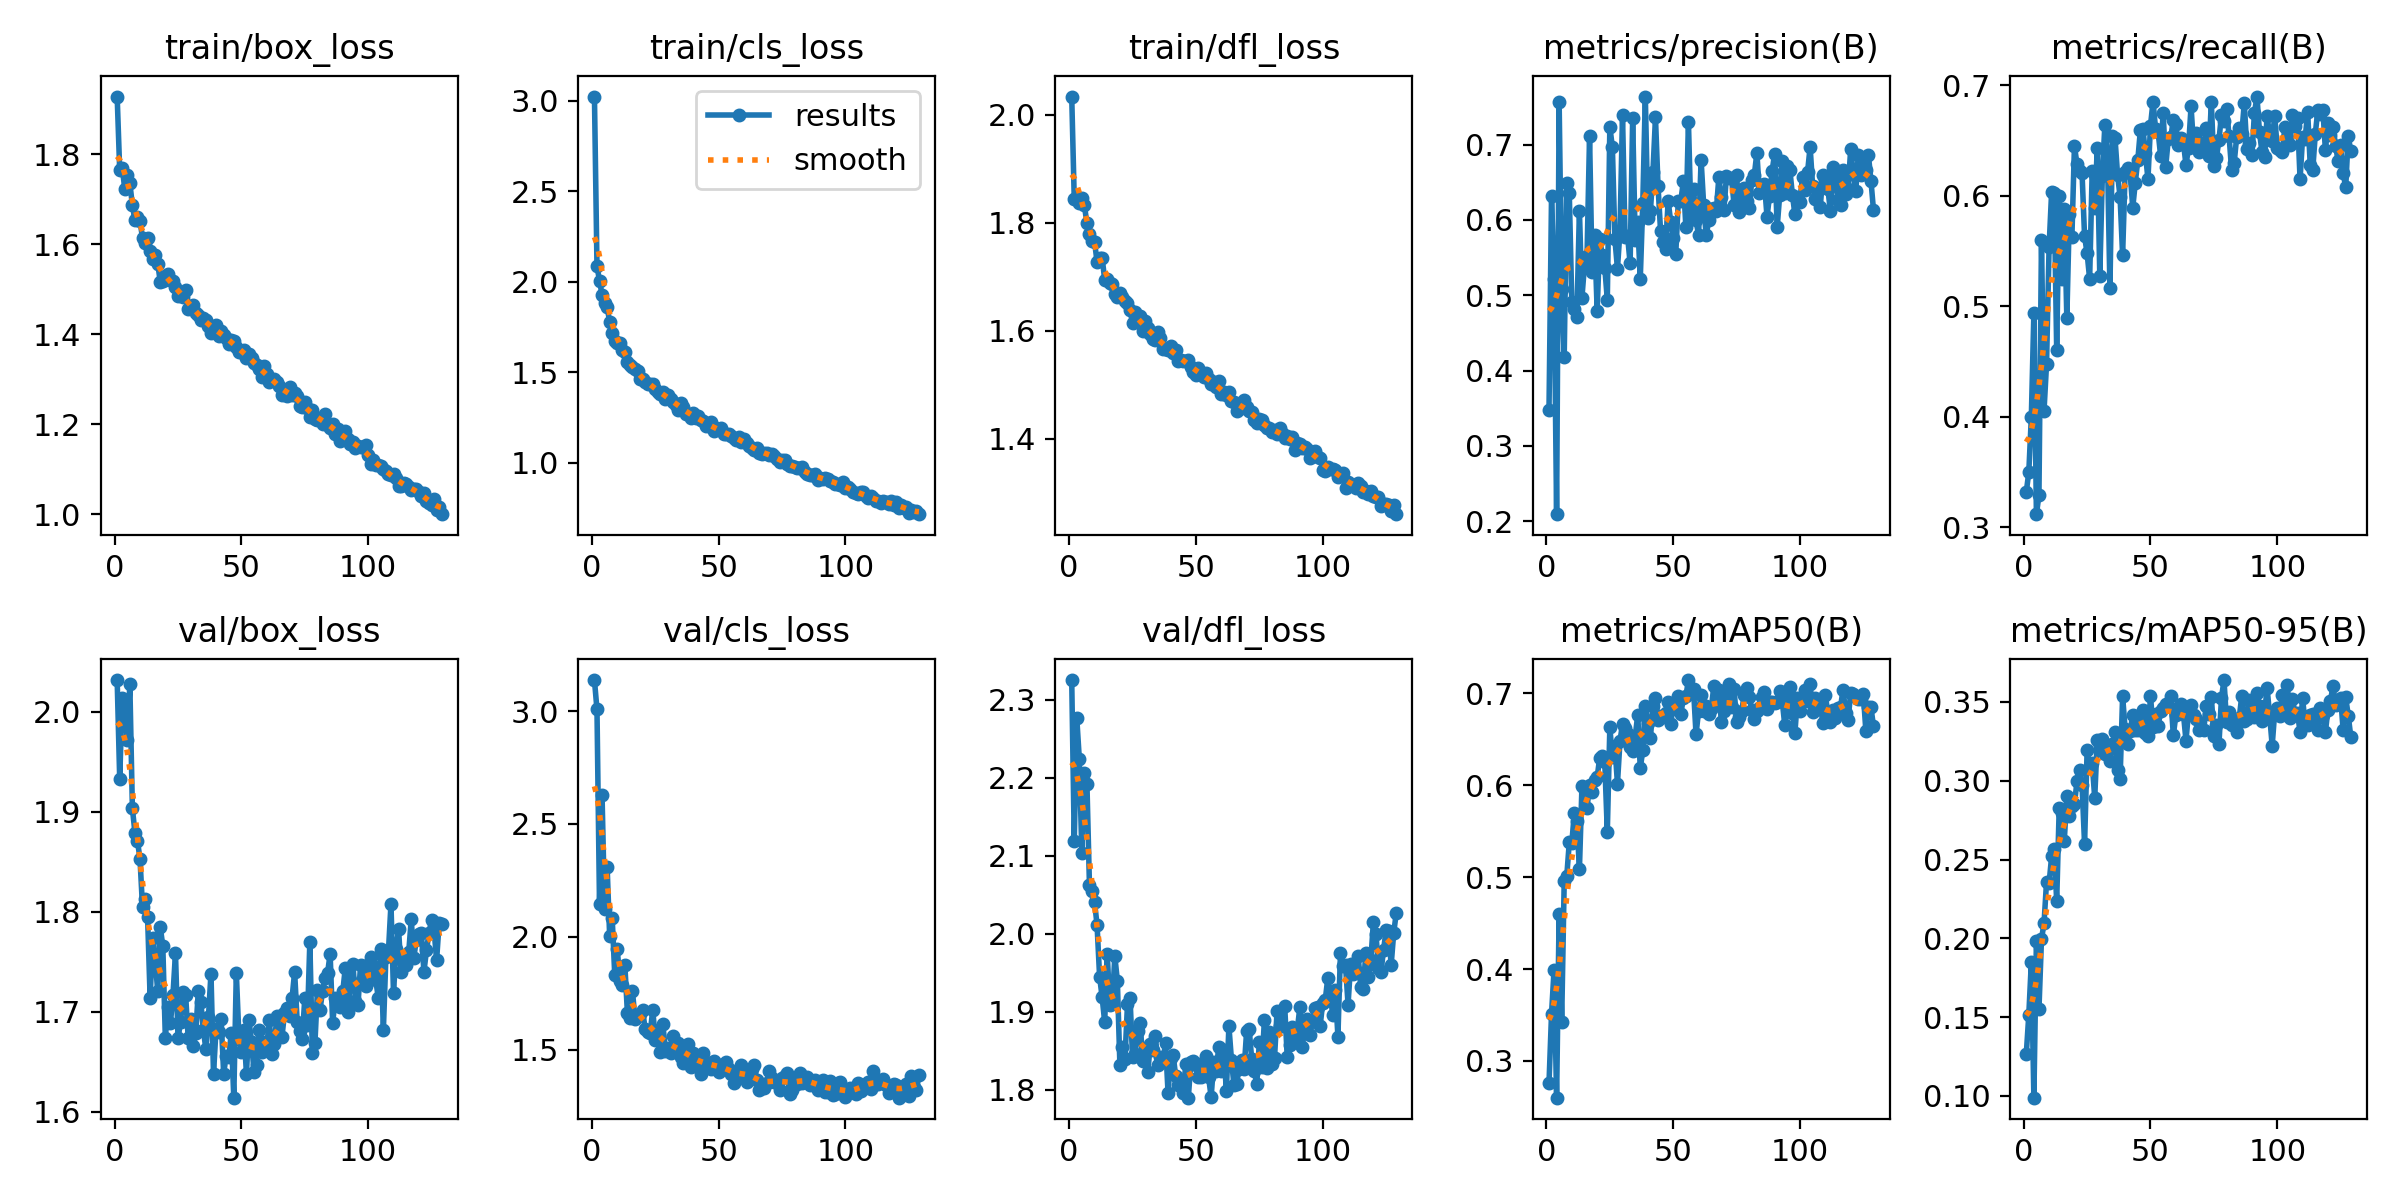
\includegraphics[width=0.9\linewidth]{img/resultsG.png}
		\caption{نمودارهای مربوط به روند آموزش مدل}
	\end{figure}
	\begin{figure}[H]
		\centering
		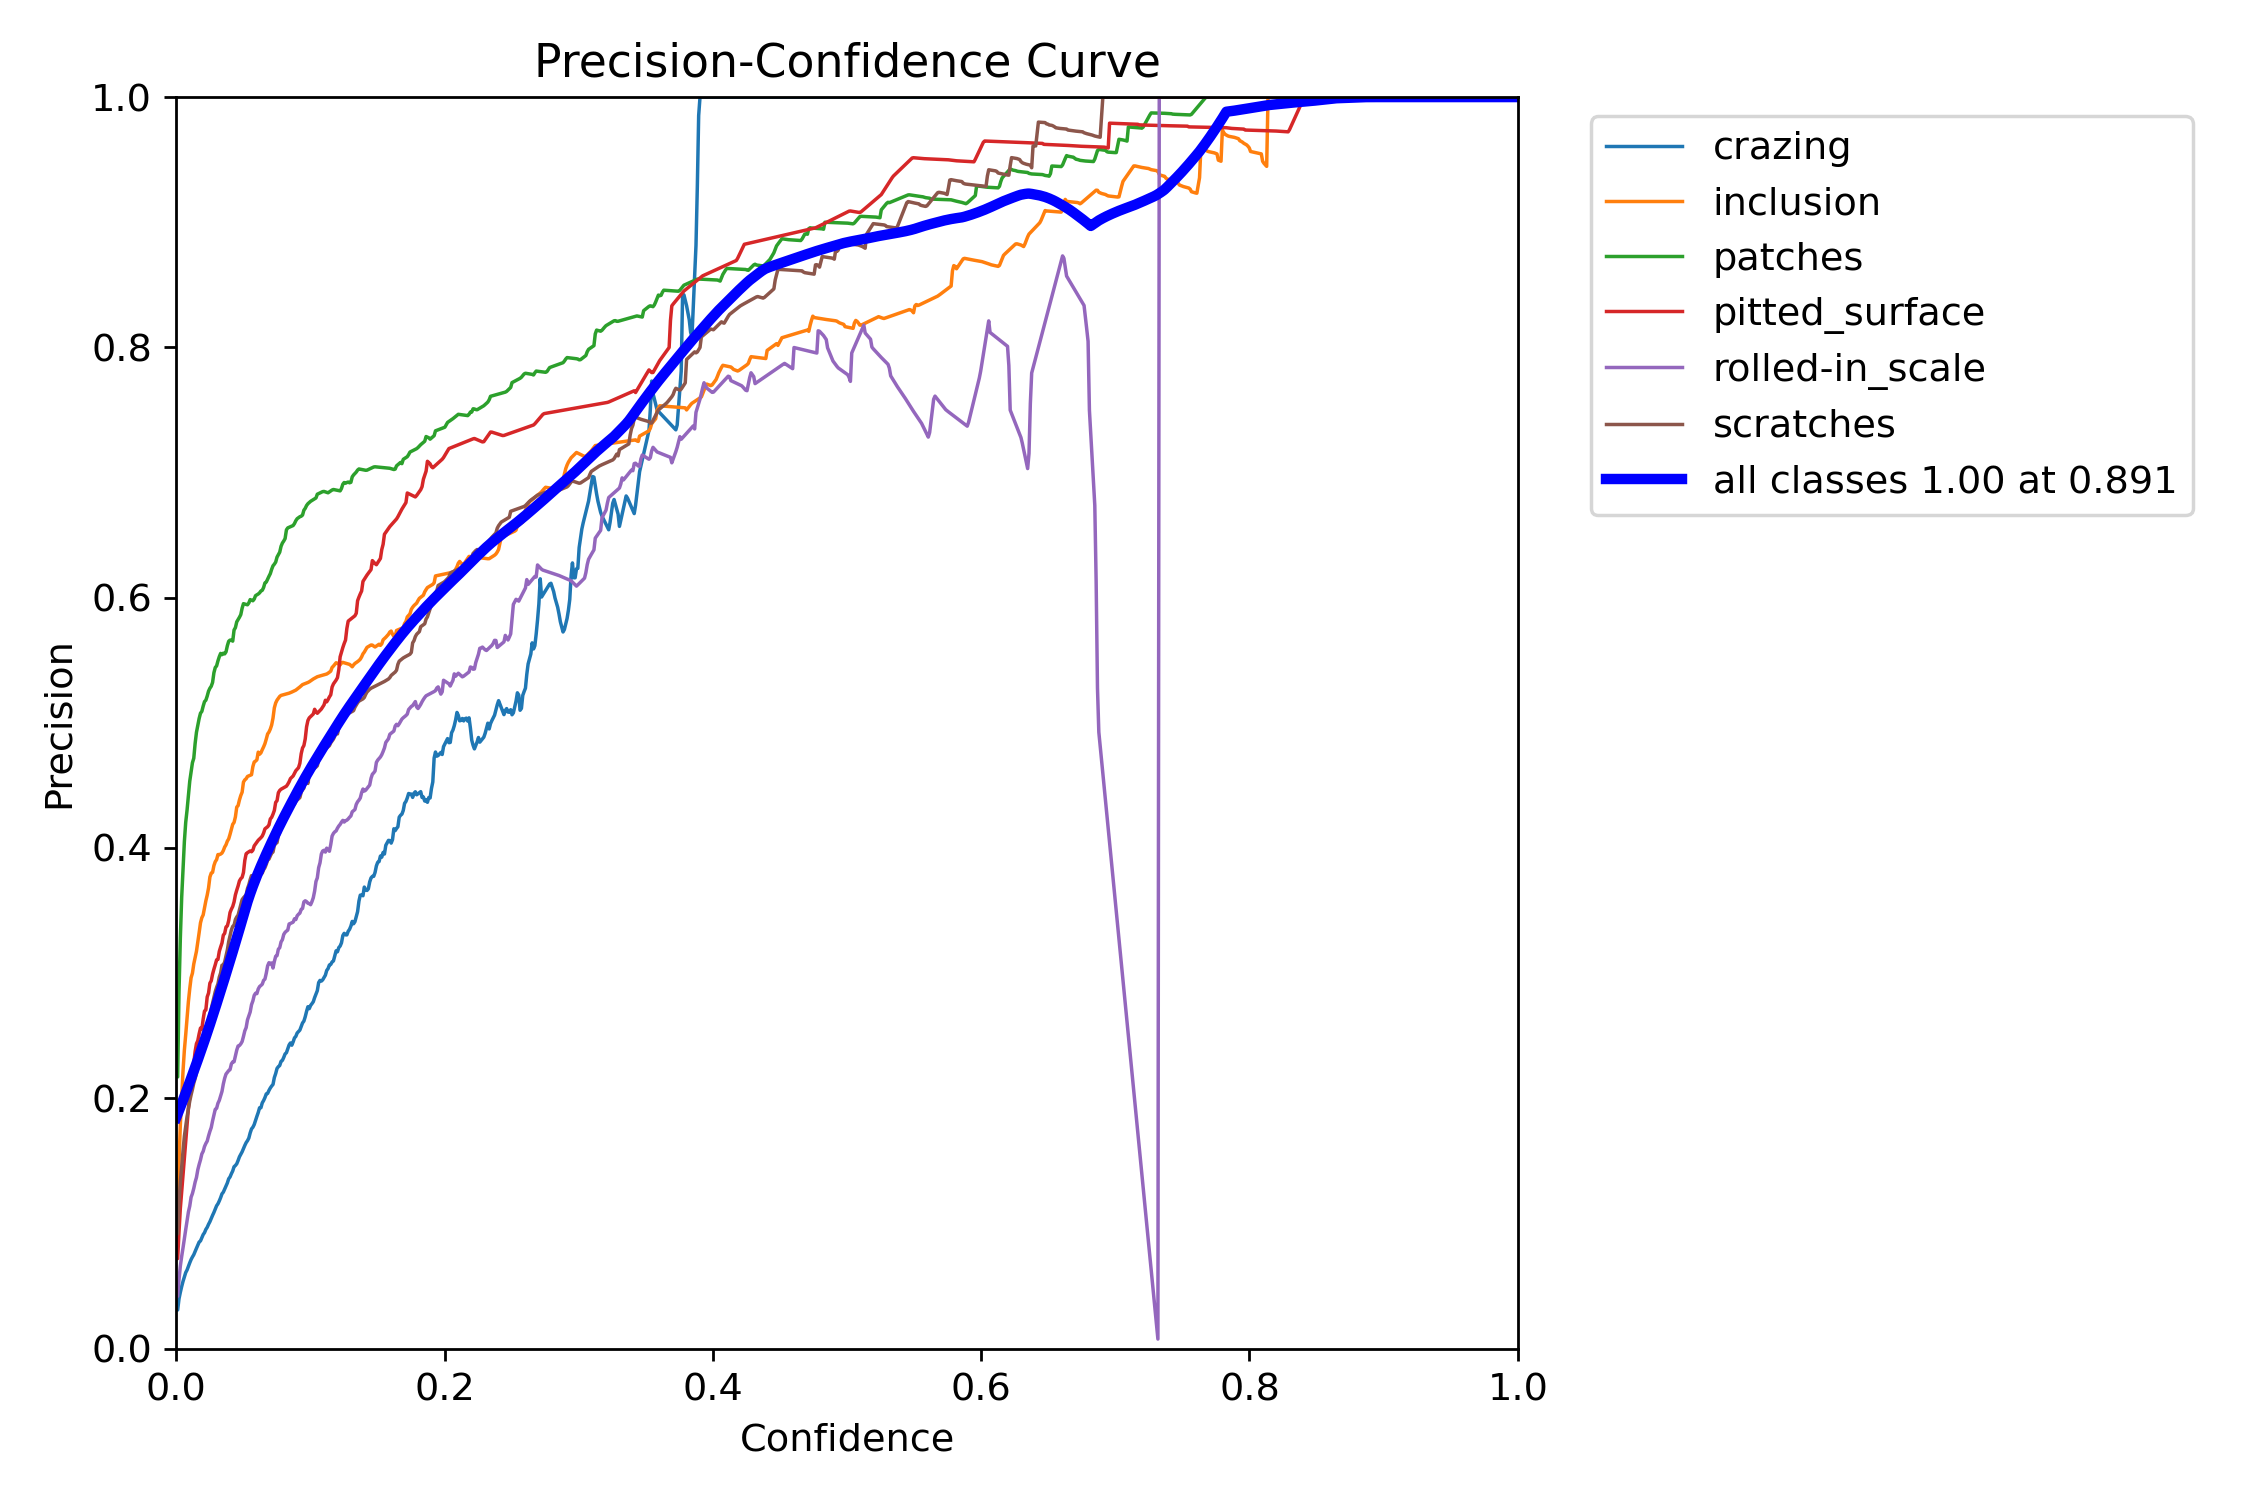
\includegraphics[width=0.45\linewidth]{img/BoxP_curveg.png}
		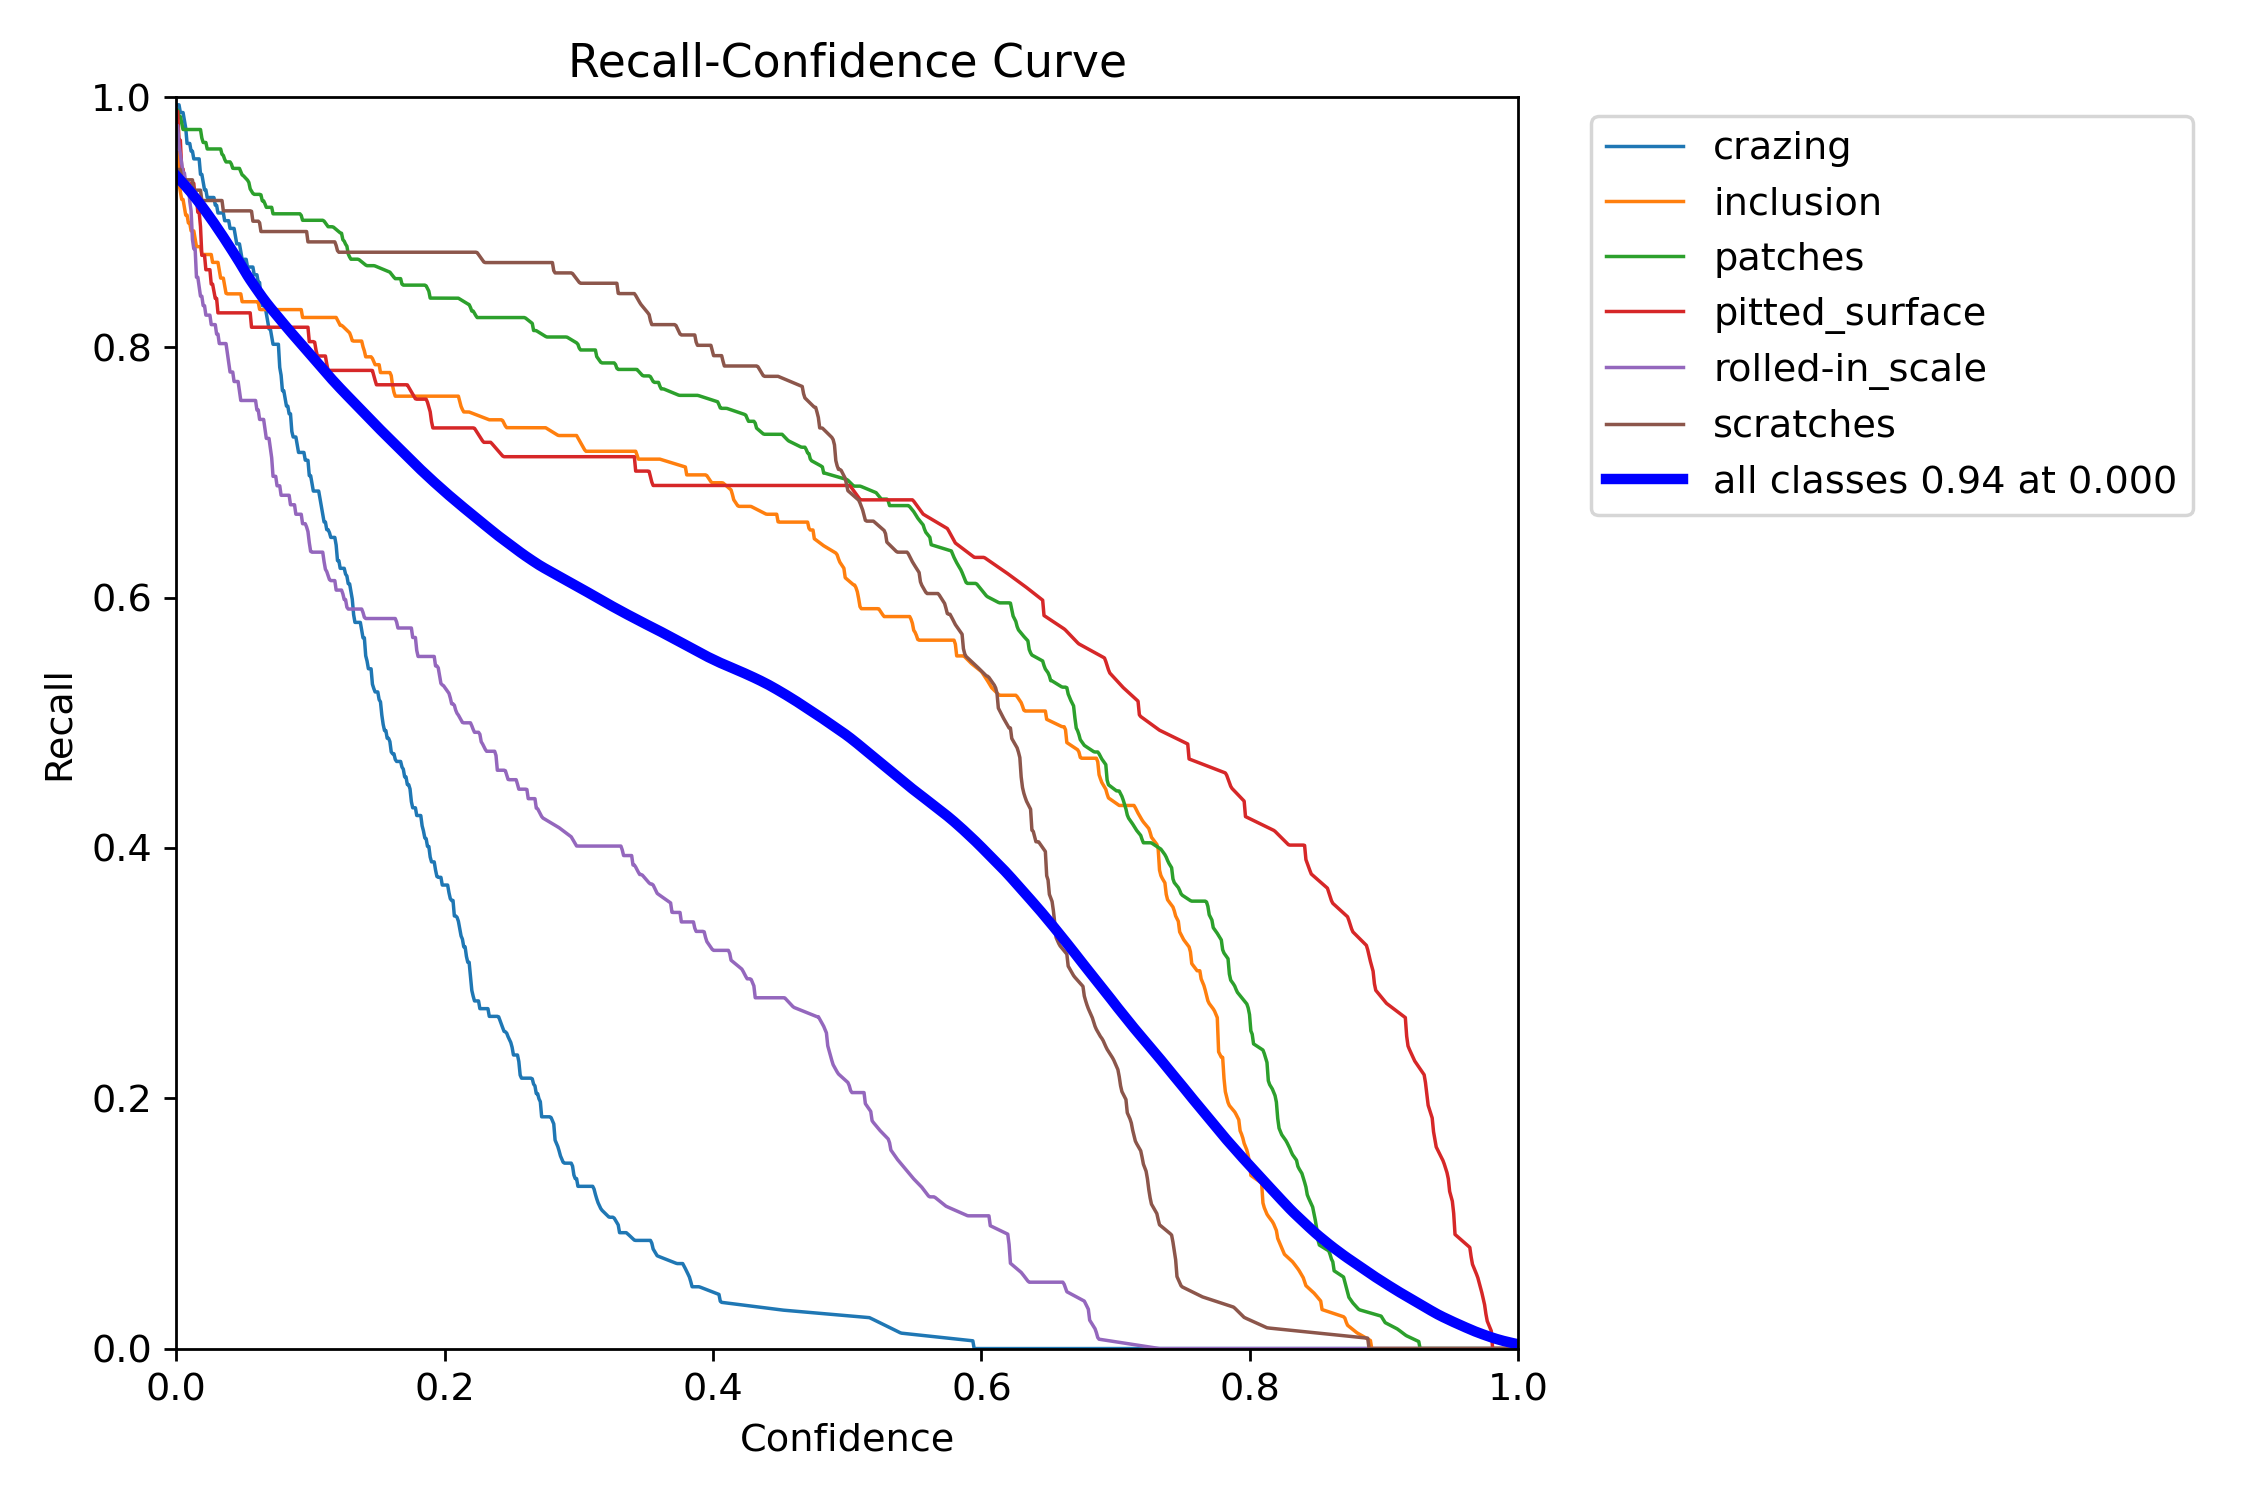
\includegraphics[width=0.45\linewidth]{img/BoxR_curveg.png}
		
		\vspace{0.3cm}
		
		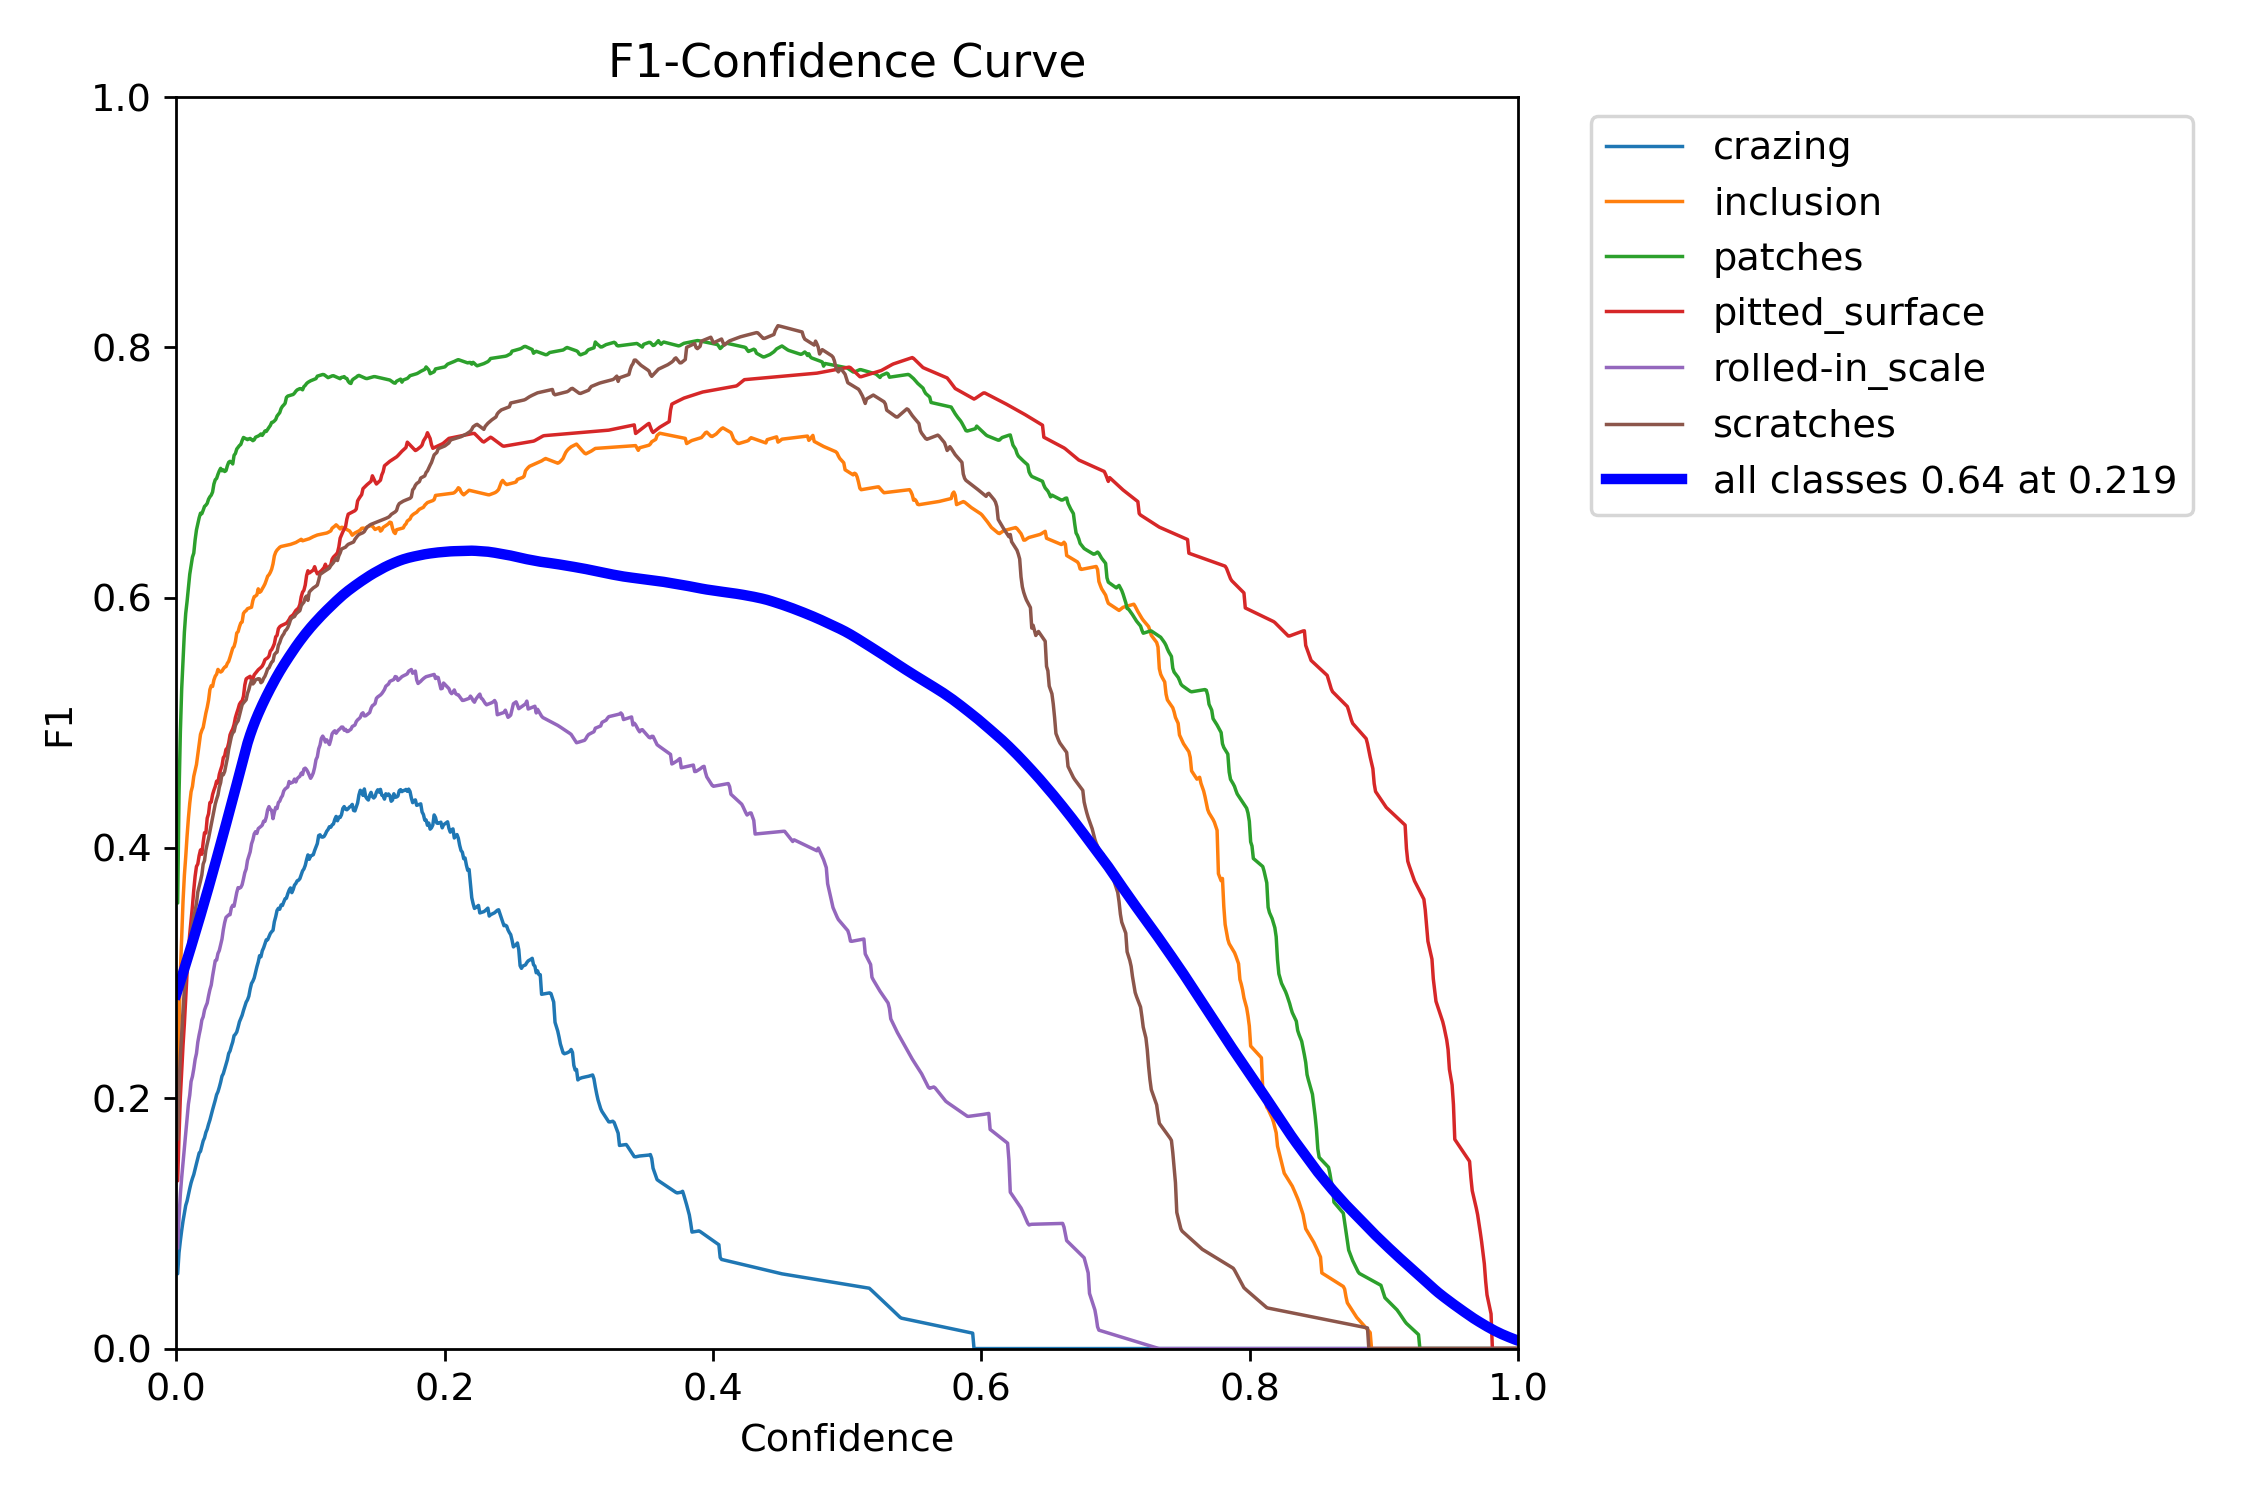
\includegraphics[width=0.45\linewidth]{img/BoxF1_curveg.png}
		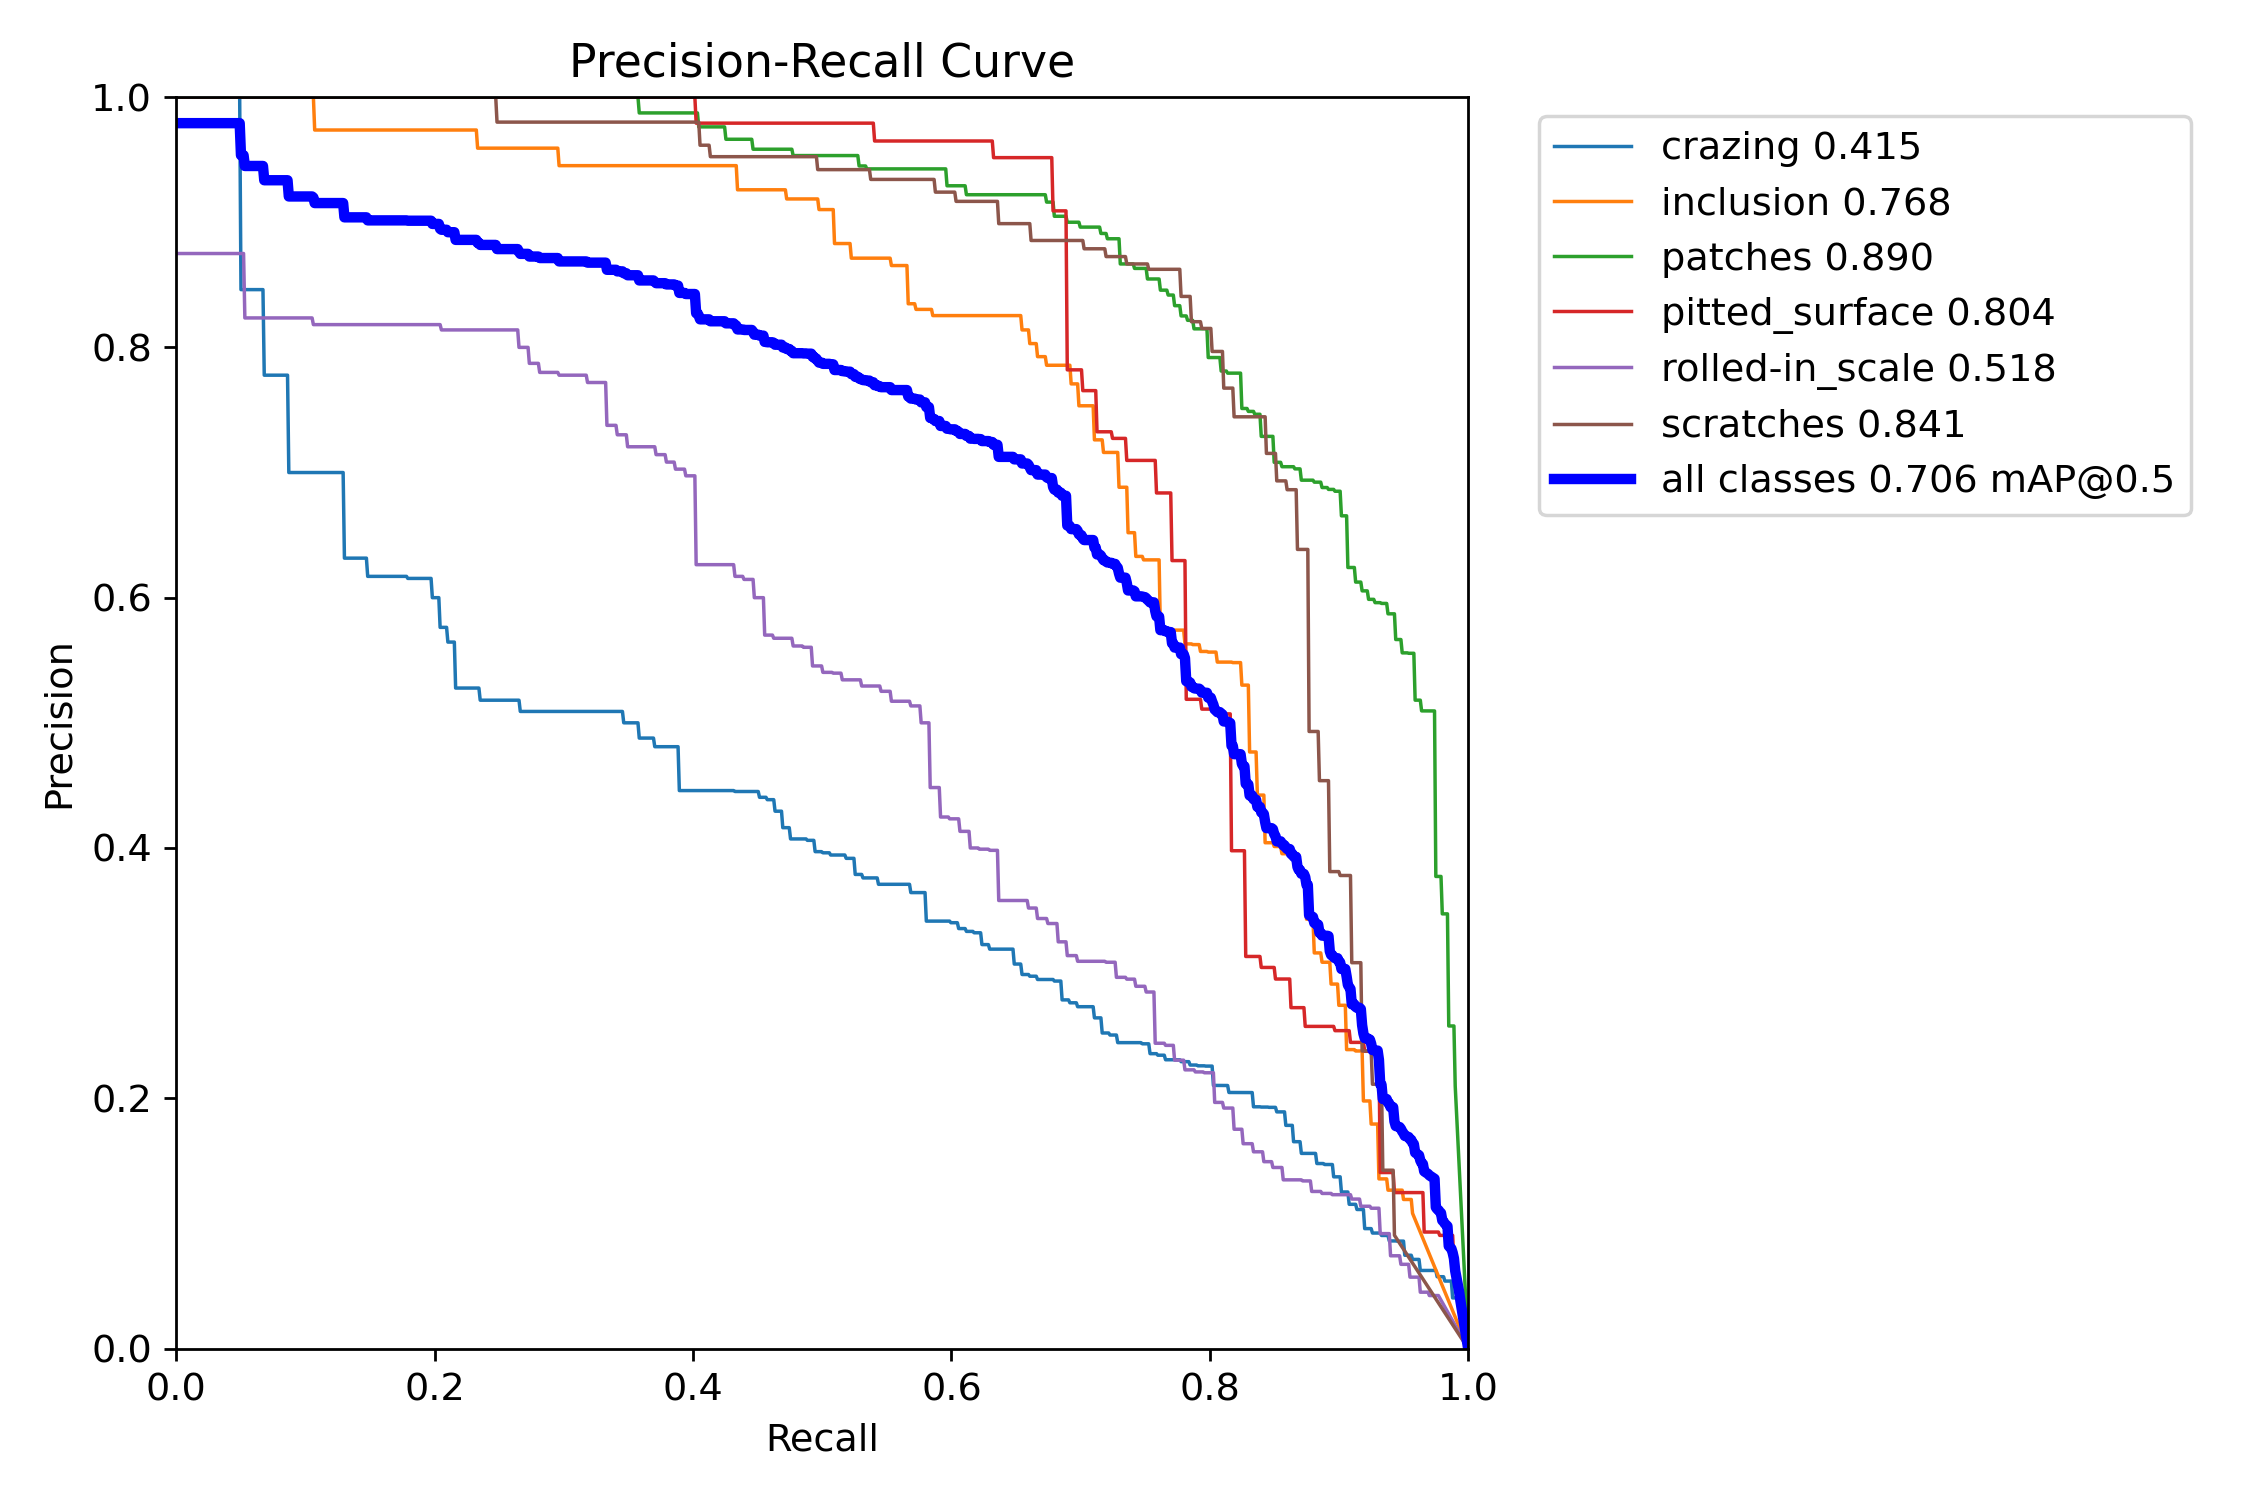
\includegraphics[width=0.45\linewidth]{img/BoxPR_curveg.png}
		\caption{نمودارهای \lr{precision}، \lr{Recall} و \lr{F1score} برحسب مقدار \lr{Confidence} و همچنین نمودار \lr{precision-Recall}}
	\end{figure}
	همانطور که در شکل نه مشخص است، مدل در بخش طبقه‌بندی به خوبی آموزش دیده و همواره مقدار ارور آن بر روی داده‌های اعتبارسنجی رو به پایین بوده است اما در کشیدن \lr{Bounding Box} دچار اورفیت شده است و از اپوک 50 به بعد مقدار ارور آن رو به افزایش رفته است.
	
	در تمامی متریک‌های دیگر نیز همانطور که از نمودار شکل سه مشخص است همواره در حال افزایش بودیم هرچند که به مقادیر آنچنان بالایی دست نیافتیم. نمودارها نشان می‌دهند که روند آموزش مدل به شیوۀ درستی صورت پذیرفته است.
	
	\paragraph{نمودار \lr{Precision} برحسب \lr{Confidence}}
	
	
	این نمودار تغییرات معیار \lr{Precision} را نسبت به آستانه اطمینان (\lr{Confidence}) نشان می‌دهد. 
	\lr{Precision} بیانگر نسبت پیش‌بینی‌های صحیح مثبت به کل پیش‌بینی‌های مثبت مدل است. 
	با افزایش مقدار \lr{Confidence}، مدل تنها نمونه‌هایی را به‌عنوان مثبت در نظر می‌گیرد که از اطمینان بالاتری برخوردارند؛ در نتیجه معمولاً مقدار \lr{Precision} افزایش می‌یابد. 
	این نمودار نشان می‌دهد که مدل تا چه حد در تشخیص نمونه‌های مثبت، از خطای پیش‌بینی مثبت کاذب جلوگیری می‌کند.
	
	\paragraph{نمودار \lr{Recall} برحسب \lr{Confidence}}
	
	
	این نمودار تغییرات معیار \lr{Recall} را برحسب مقدار \lr{Confidence} نمایش می‌دهد.
	\lr{Recall} نشان‌دهنده نسبت نمونه‌های مثبت شناسایی‌شده توسط مدل به کل نمونه‌های مثبت واقعی است.
	با افزایش آستانه \lr{Confidence}، مدل سخت‌گیرانه‌تر عمل کرده و ممکن است برخی نمونه‌های مثبت واقعی را شناسایی نکند؛ در نتیجه مقدار \lr{Recall} معمولاً کاهش می‌یابد.
	این نمودار توانایی مدل در پوشش دادن تمام نمونه‌های مثبت را نشان می‌دهد.
	
	\paragraph{نمودار \lr{F1-score} برحسب \lr{Confidence}}
	
	
	نمودار \lr{F1-score} تغییرات میانگین هارمونیک معیارهای \lr{Precision} و \lr{Recall} را نسبت به مقدار \lr{Confidence} نشان می‌دهد.
	این معیار تعادلی بین دقت و فراخوانی ایجاد می‌کند و زمانی مقدار بالایی دارد که هر دو معیار \lr{Precision} و \lr{Recall} مناسب باشند.
	این نمودار برای انتخاب آستانه \lr{Confidence} بهینه، که در آن عملکرد کلی مدل متعادل است، بسیار کاربردی می‌باشد.
	
	\paragraph{نمودار \lr{Precision-Recall}}
	
	
	نمودار \lr{Precision-Recall} رابطه بین دو معیار \lr{Precision} و \lr{Recall} را برای آستانه‌های مختلف \lr{Confidence} نمایش می‌دهد.
	این نمودار نشان می‌دهد که با افزایش \lr{Recall} (شناسایی نمونه‌های مثبت بیشتر)، معمولاً مقدار \lr{Precision} کاهش می‌یابد.
	نمودار \lr{Precision-Recall} به‌ویژه در مجموعه‌داده‌های نامتوازن اهمیت زیادی دارد و عملکرد مدل را در تشخیص کلاس مثبت به‌صورت جامع ارزیابی می‌کند.
	هرچه منحنی به ناحیه بالا-راست نزدیک‌تر باشد، عملکرد مدل مطلوب‌تر است.
	
	از این نمودارها نتیجه می‌گیریم که روی دو کلاس \lr{Crazing} و \lr{rolled in scale} نتایج چندان خوب نیست و پایین است. روی کلاس‌های \lr{Patches} و \lr{Pitted surface} نتایج بالاتر و بهتر است.
	
	در بخش طبقه‌بندی نیز دو ماتریس درهمریختگی ترسیم شده است که در شکل‌های زیر قابل مشاهده است:
	\begin{figure}[H]
		\centering
		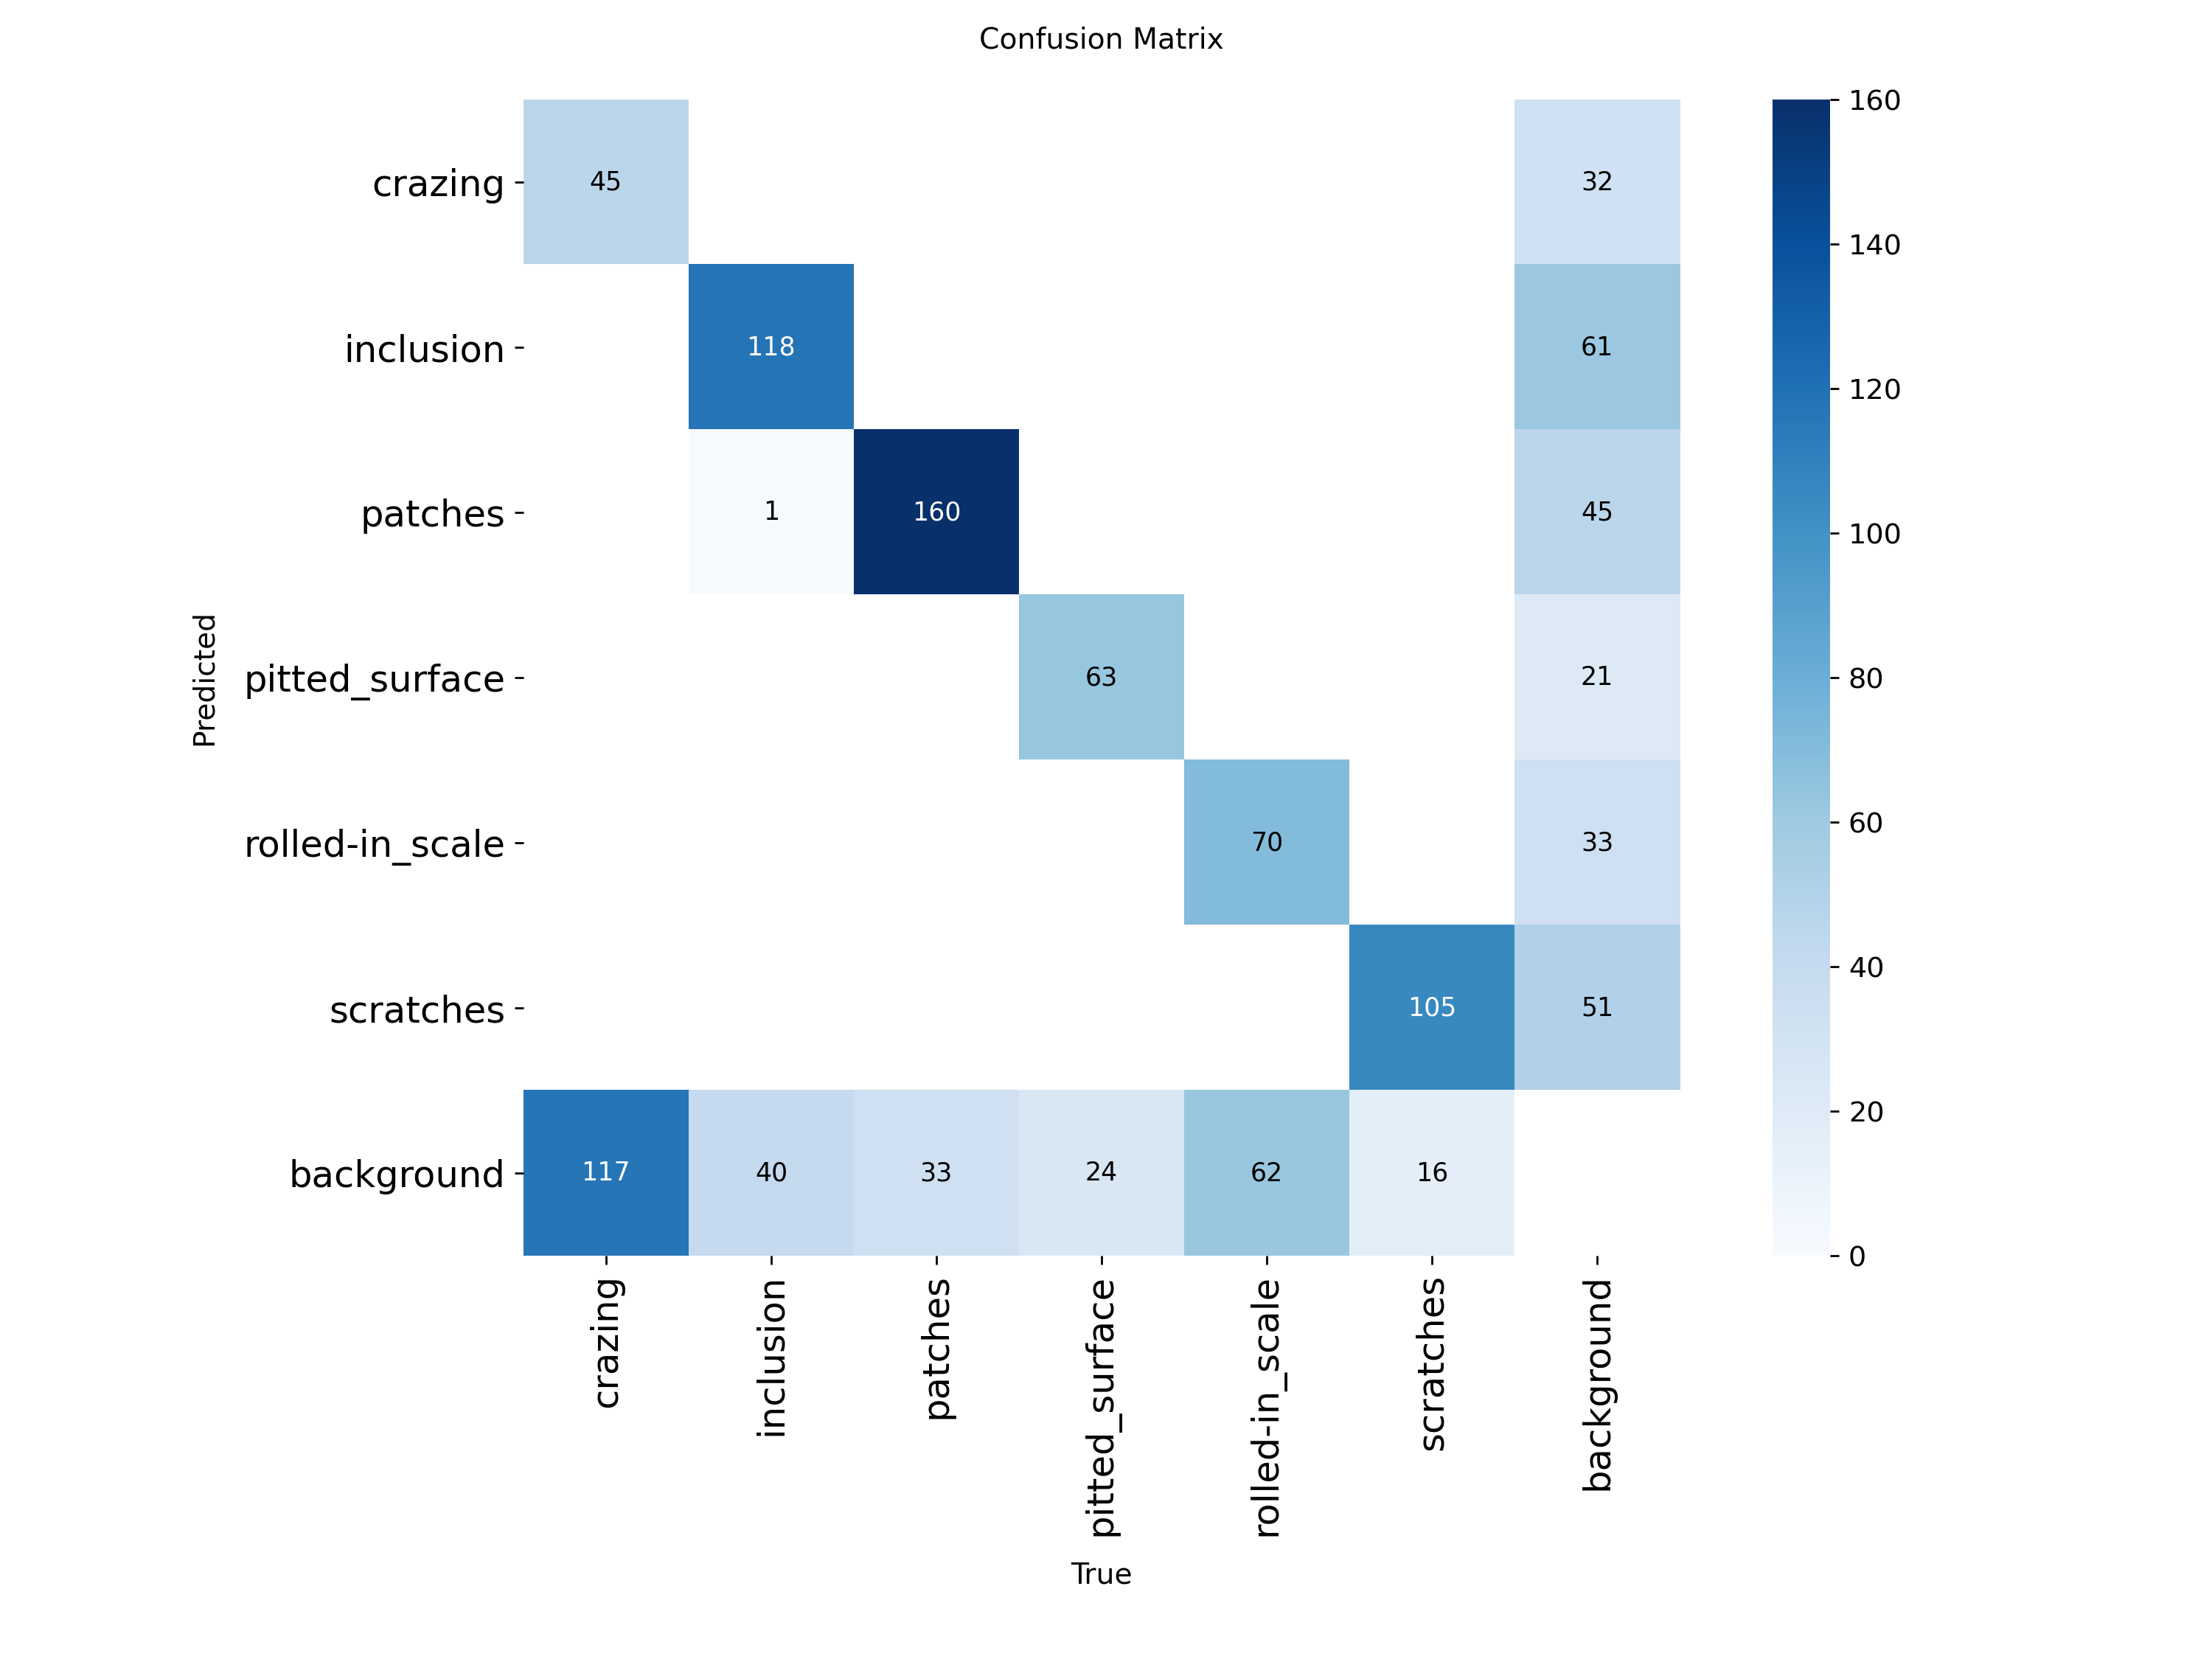
\includegraphics[width=0.3\linewidth]{img/confusion_matrixg.png}
		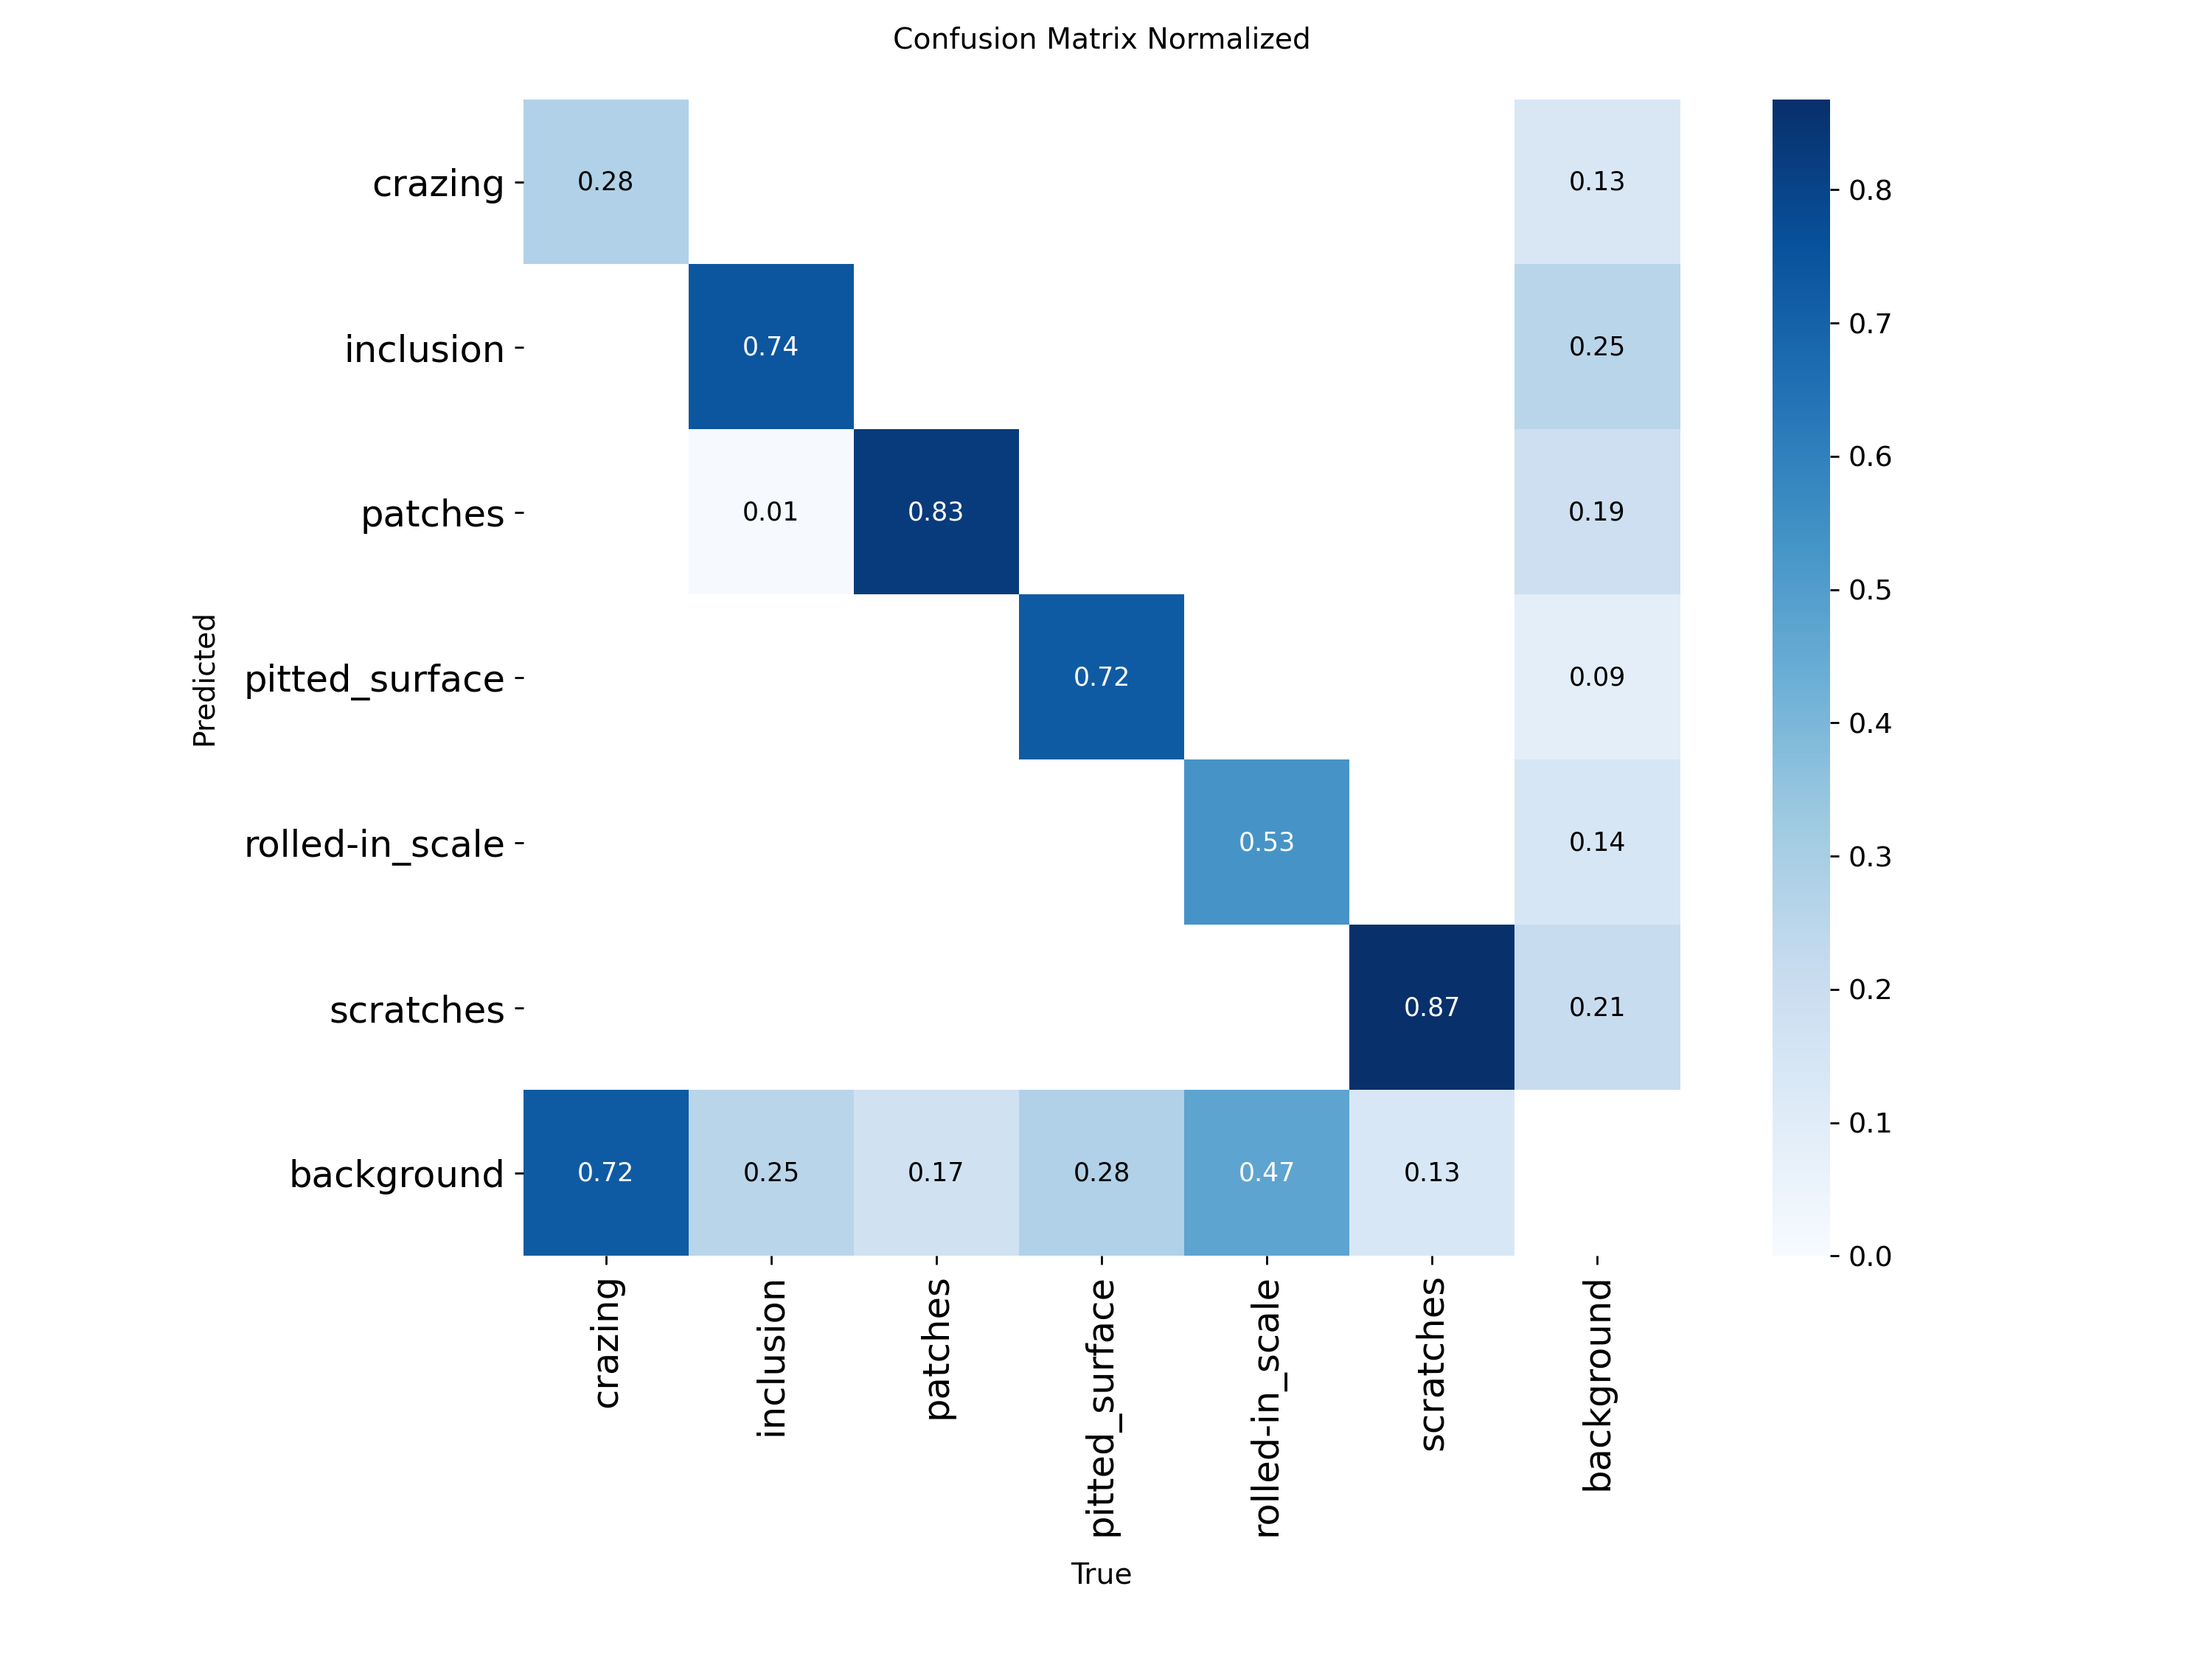
\includegraphics[width=0.3\linewidth]{img/confusion_matrix_normalizedg.png}
		\caption{ماتریس درهمریختگی}
	\end{figure}
	همانطور که مشخص است مدل در تشخیص قسمت پس‌زمینه خیلی خطا می‌کند و جاهایی رو به عنوان خرابی اعلام می‌کند که واقعا خرابی در آنجا نیست. نکته قابل تامل این است که مدل در تشخیص بین دو کلاس خطایی نداشته و فقط یک مورد خطا داشته است. این یعنی ما کلاسی نداشتیم که به اشتباه چیز دیگری تشخیص دهیم و هرجا هم اشتباهی رخ داده فقط این بوده که اونجا خرابی نبوده است و مدل آن را خراب تشخیص داده است. بنظر می‌آید که اگر پیش‌پردازش را بهتر کنیم و بتوانیم بهتر ناحیه پس‌زمینه را از کلاس‌ها جدا کنیم، نتایج بهتری به دست می‌آوریم. همچنین می‌توانیم ساختار مدل را بهبود بدهیم و یا از مدل‌های \lr{YOLO} با ورژن بالاتر استفاده نماییم که در ادامه این امر تحقق پیدا کرده است.
	
	در شکل زیر نمونه از \lr{Batch}های \lr{Validation} آورده شده است که تشخیص مدل را نشان می‌دهد:
	\begin{figure}[H]
		\centering
		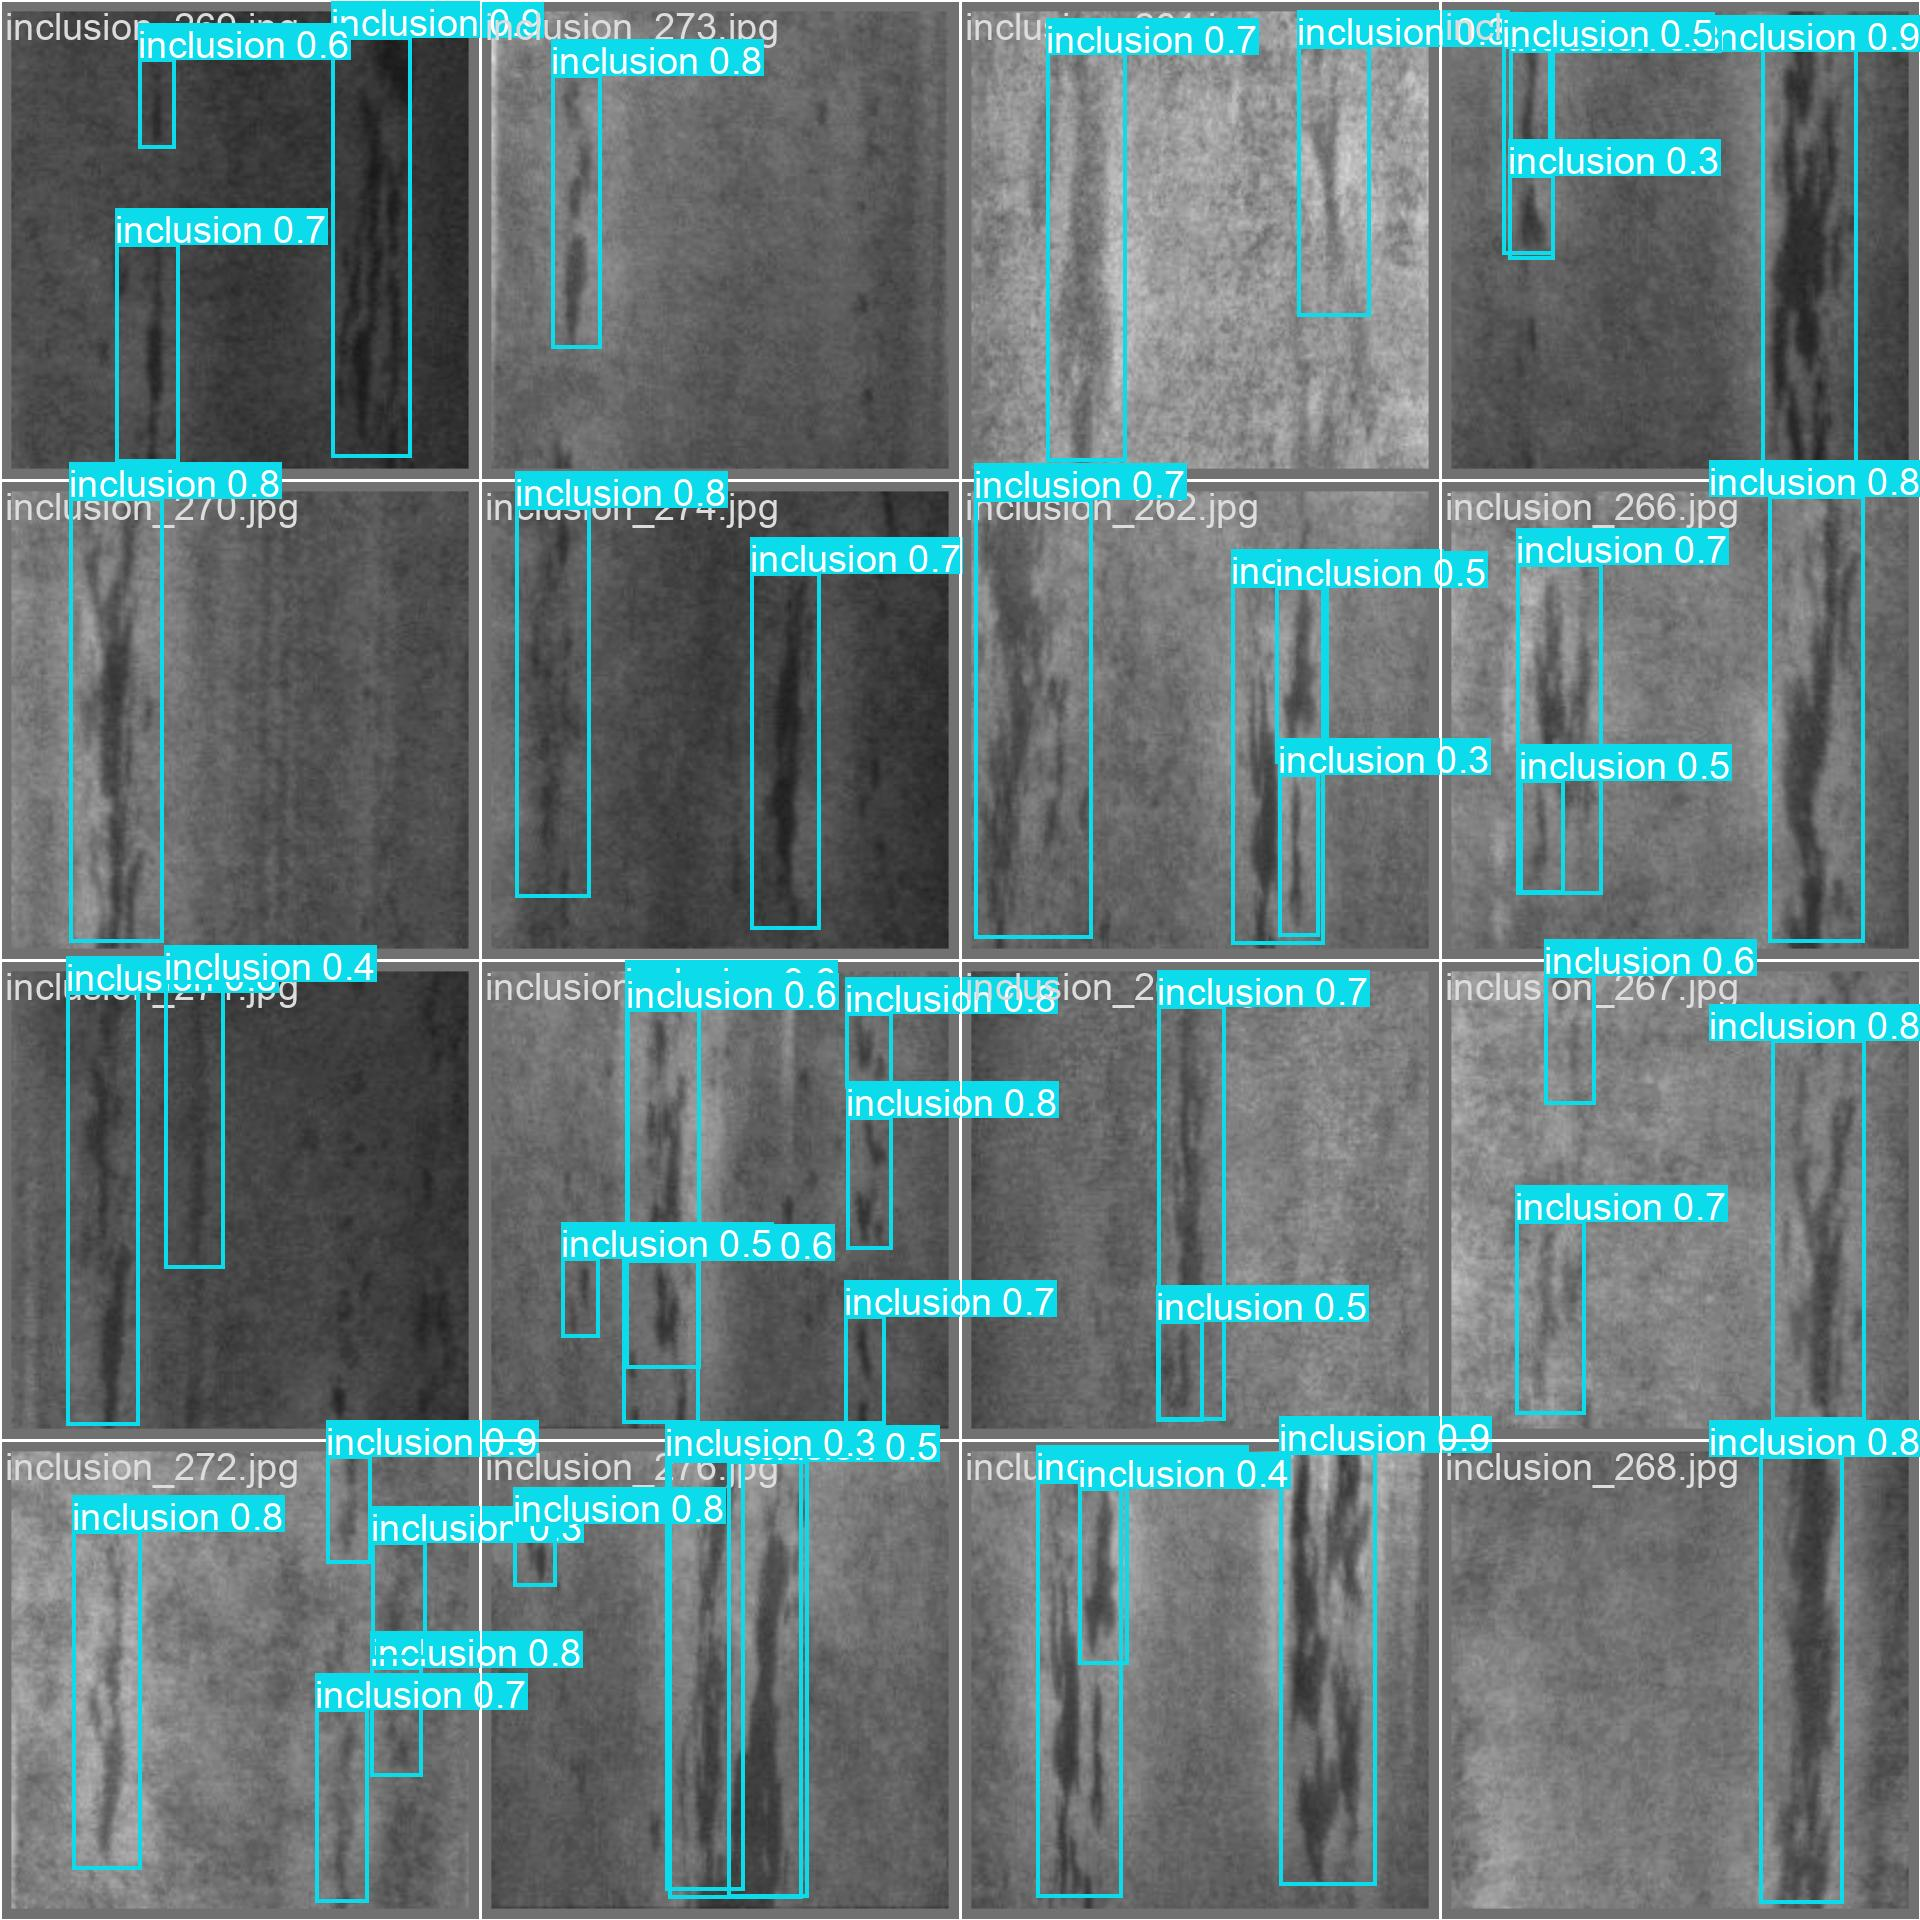
\includegraphics[width=0.2\linewidth]{img/val_batch2_predg.jpg}
		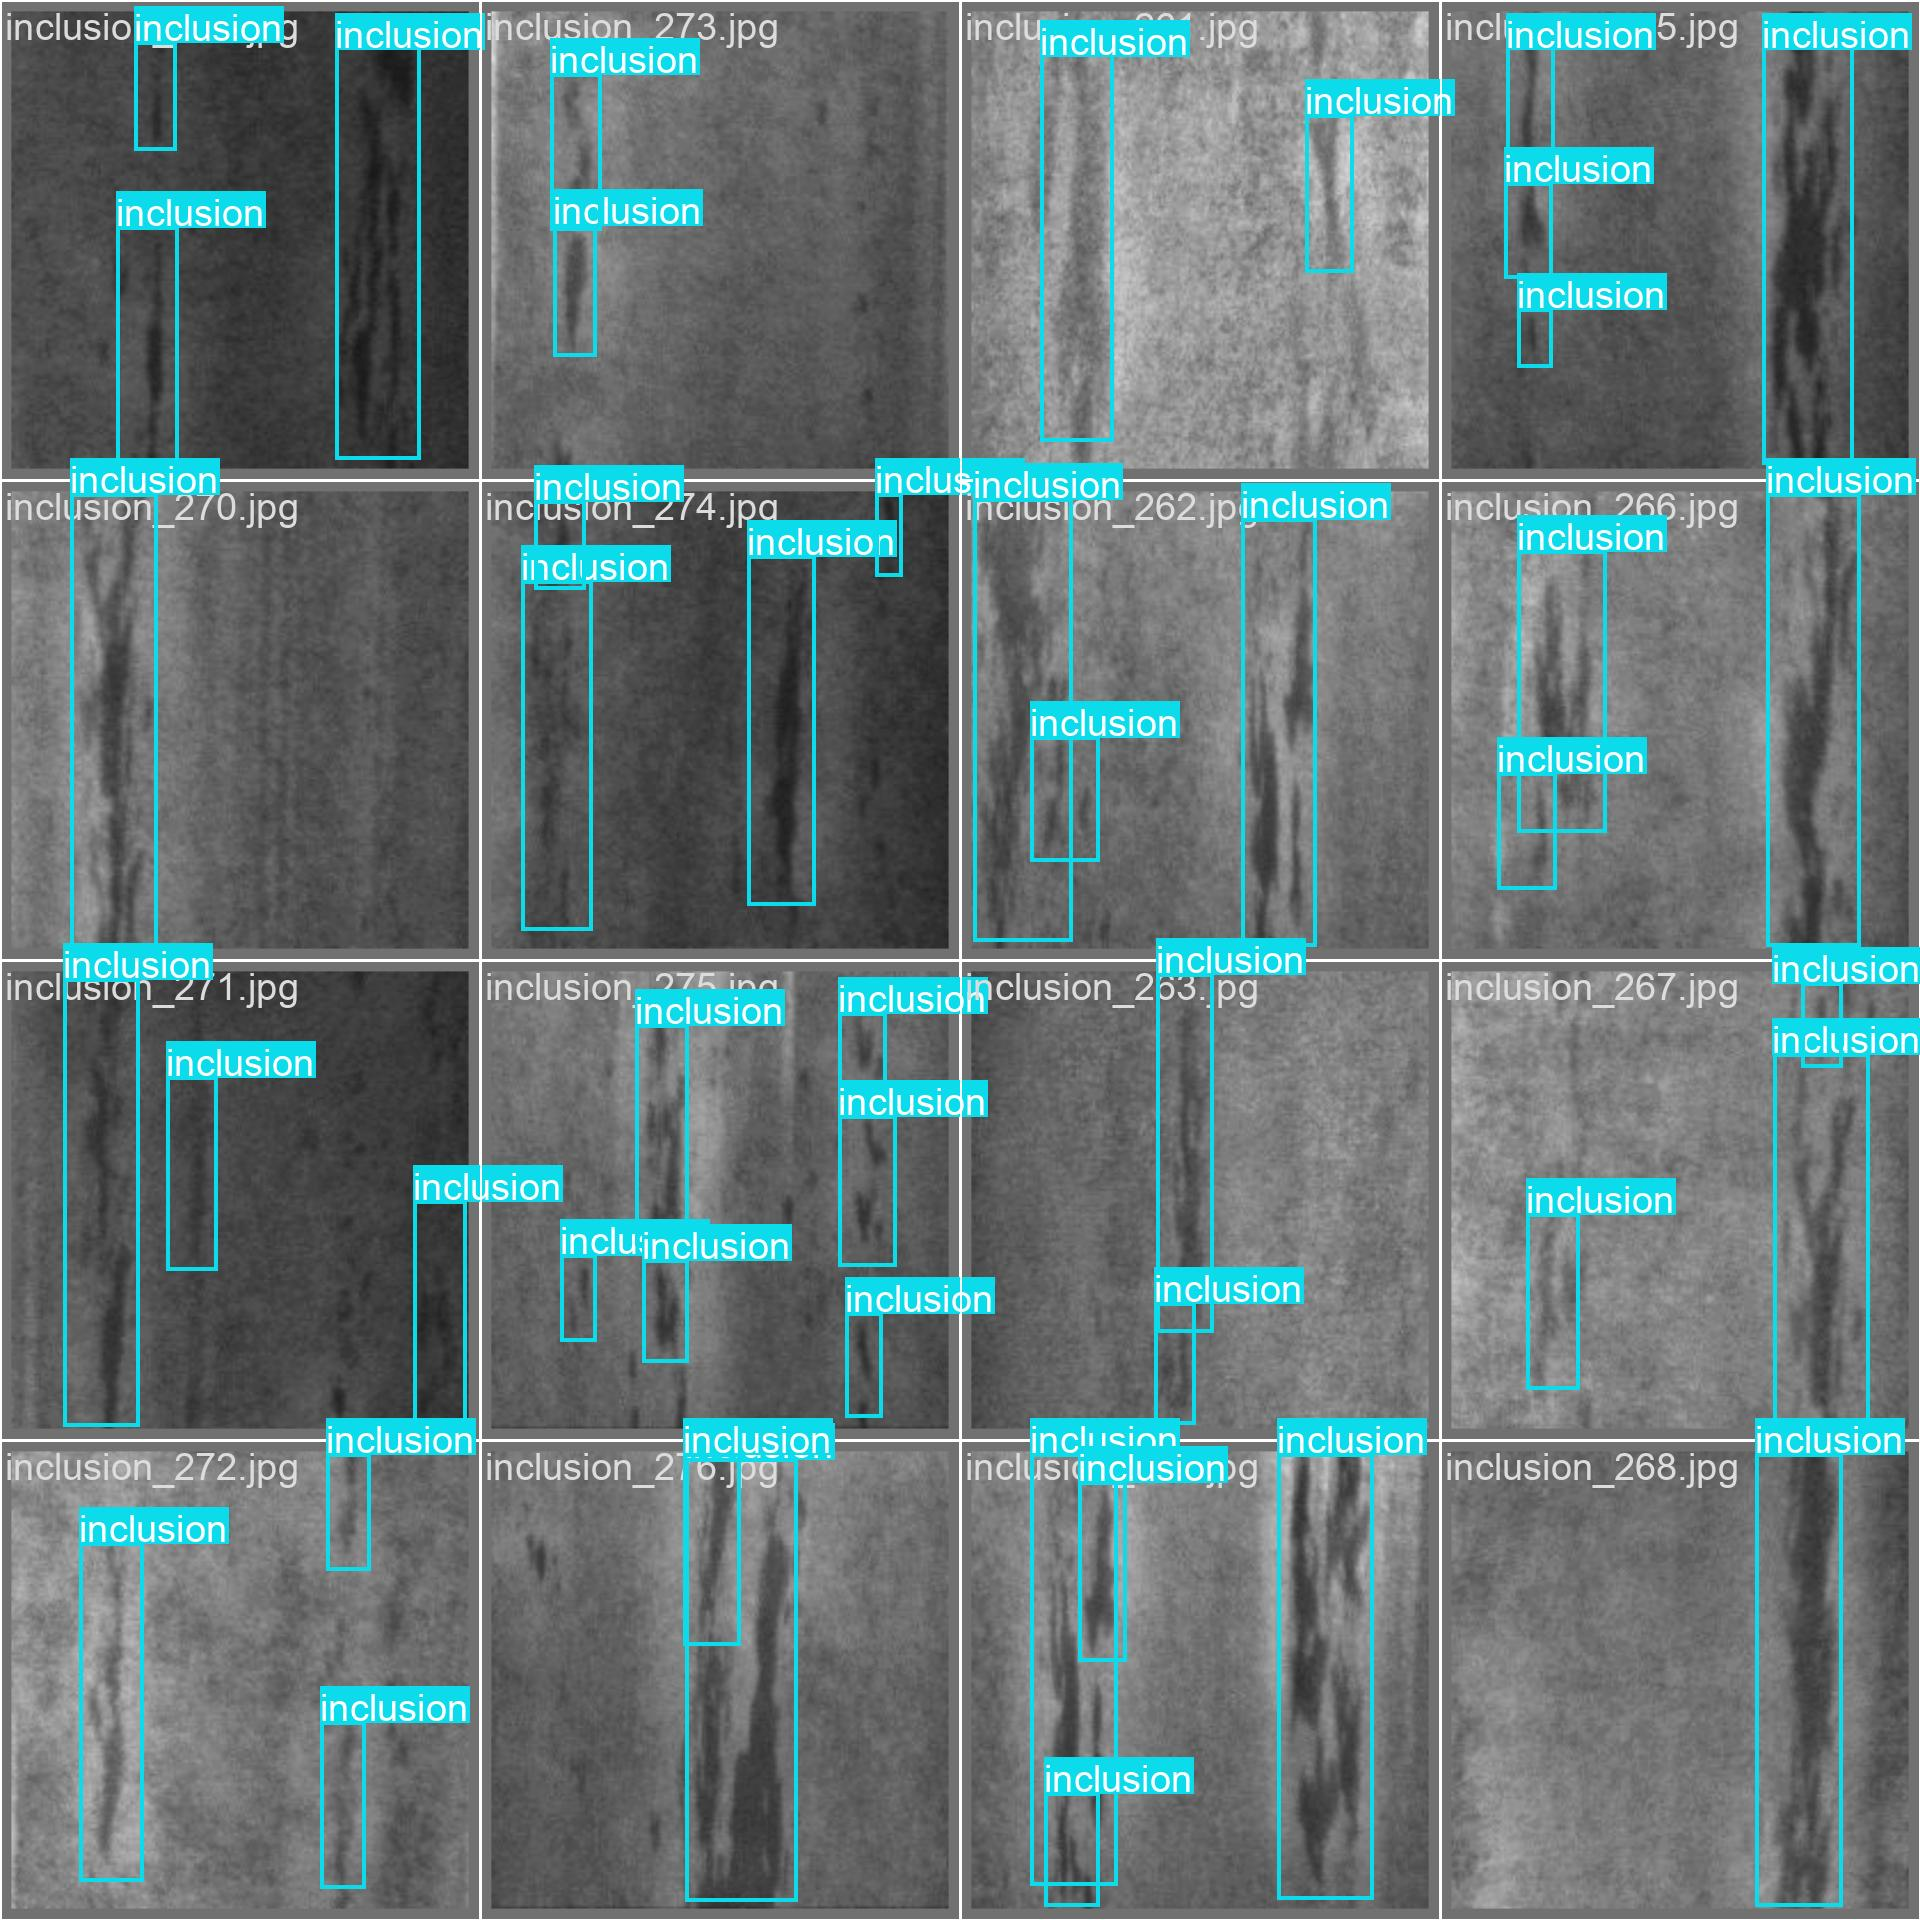
\includegraphics[width=0.2\linewidth]{img/val_batch2_labelsg.jpg}
		
		\vspace{0.3cm}
		
		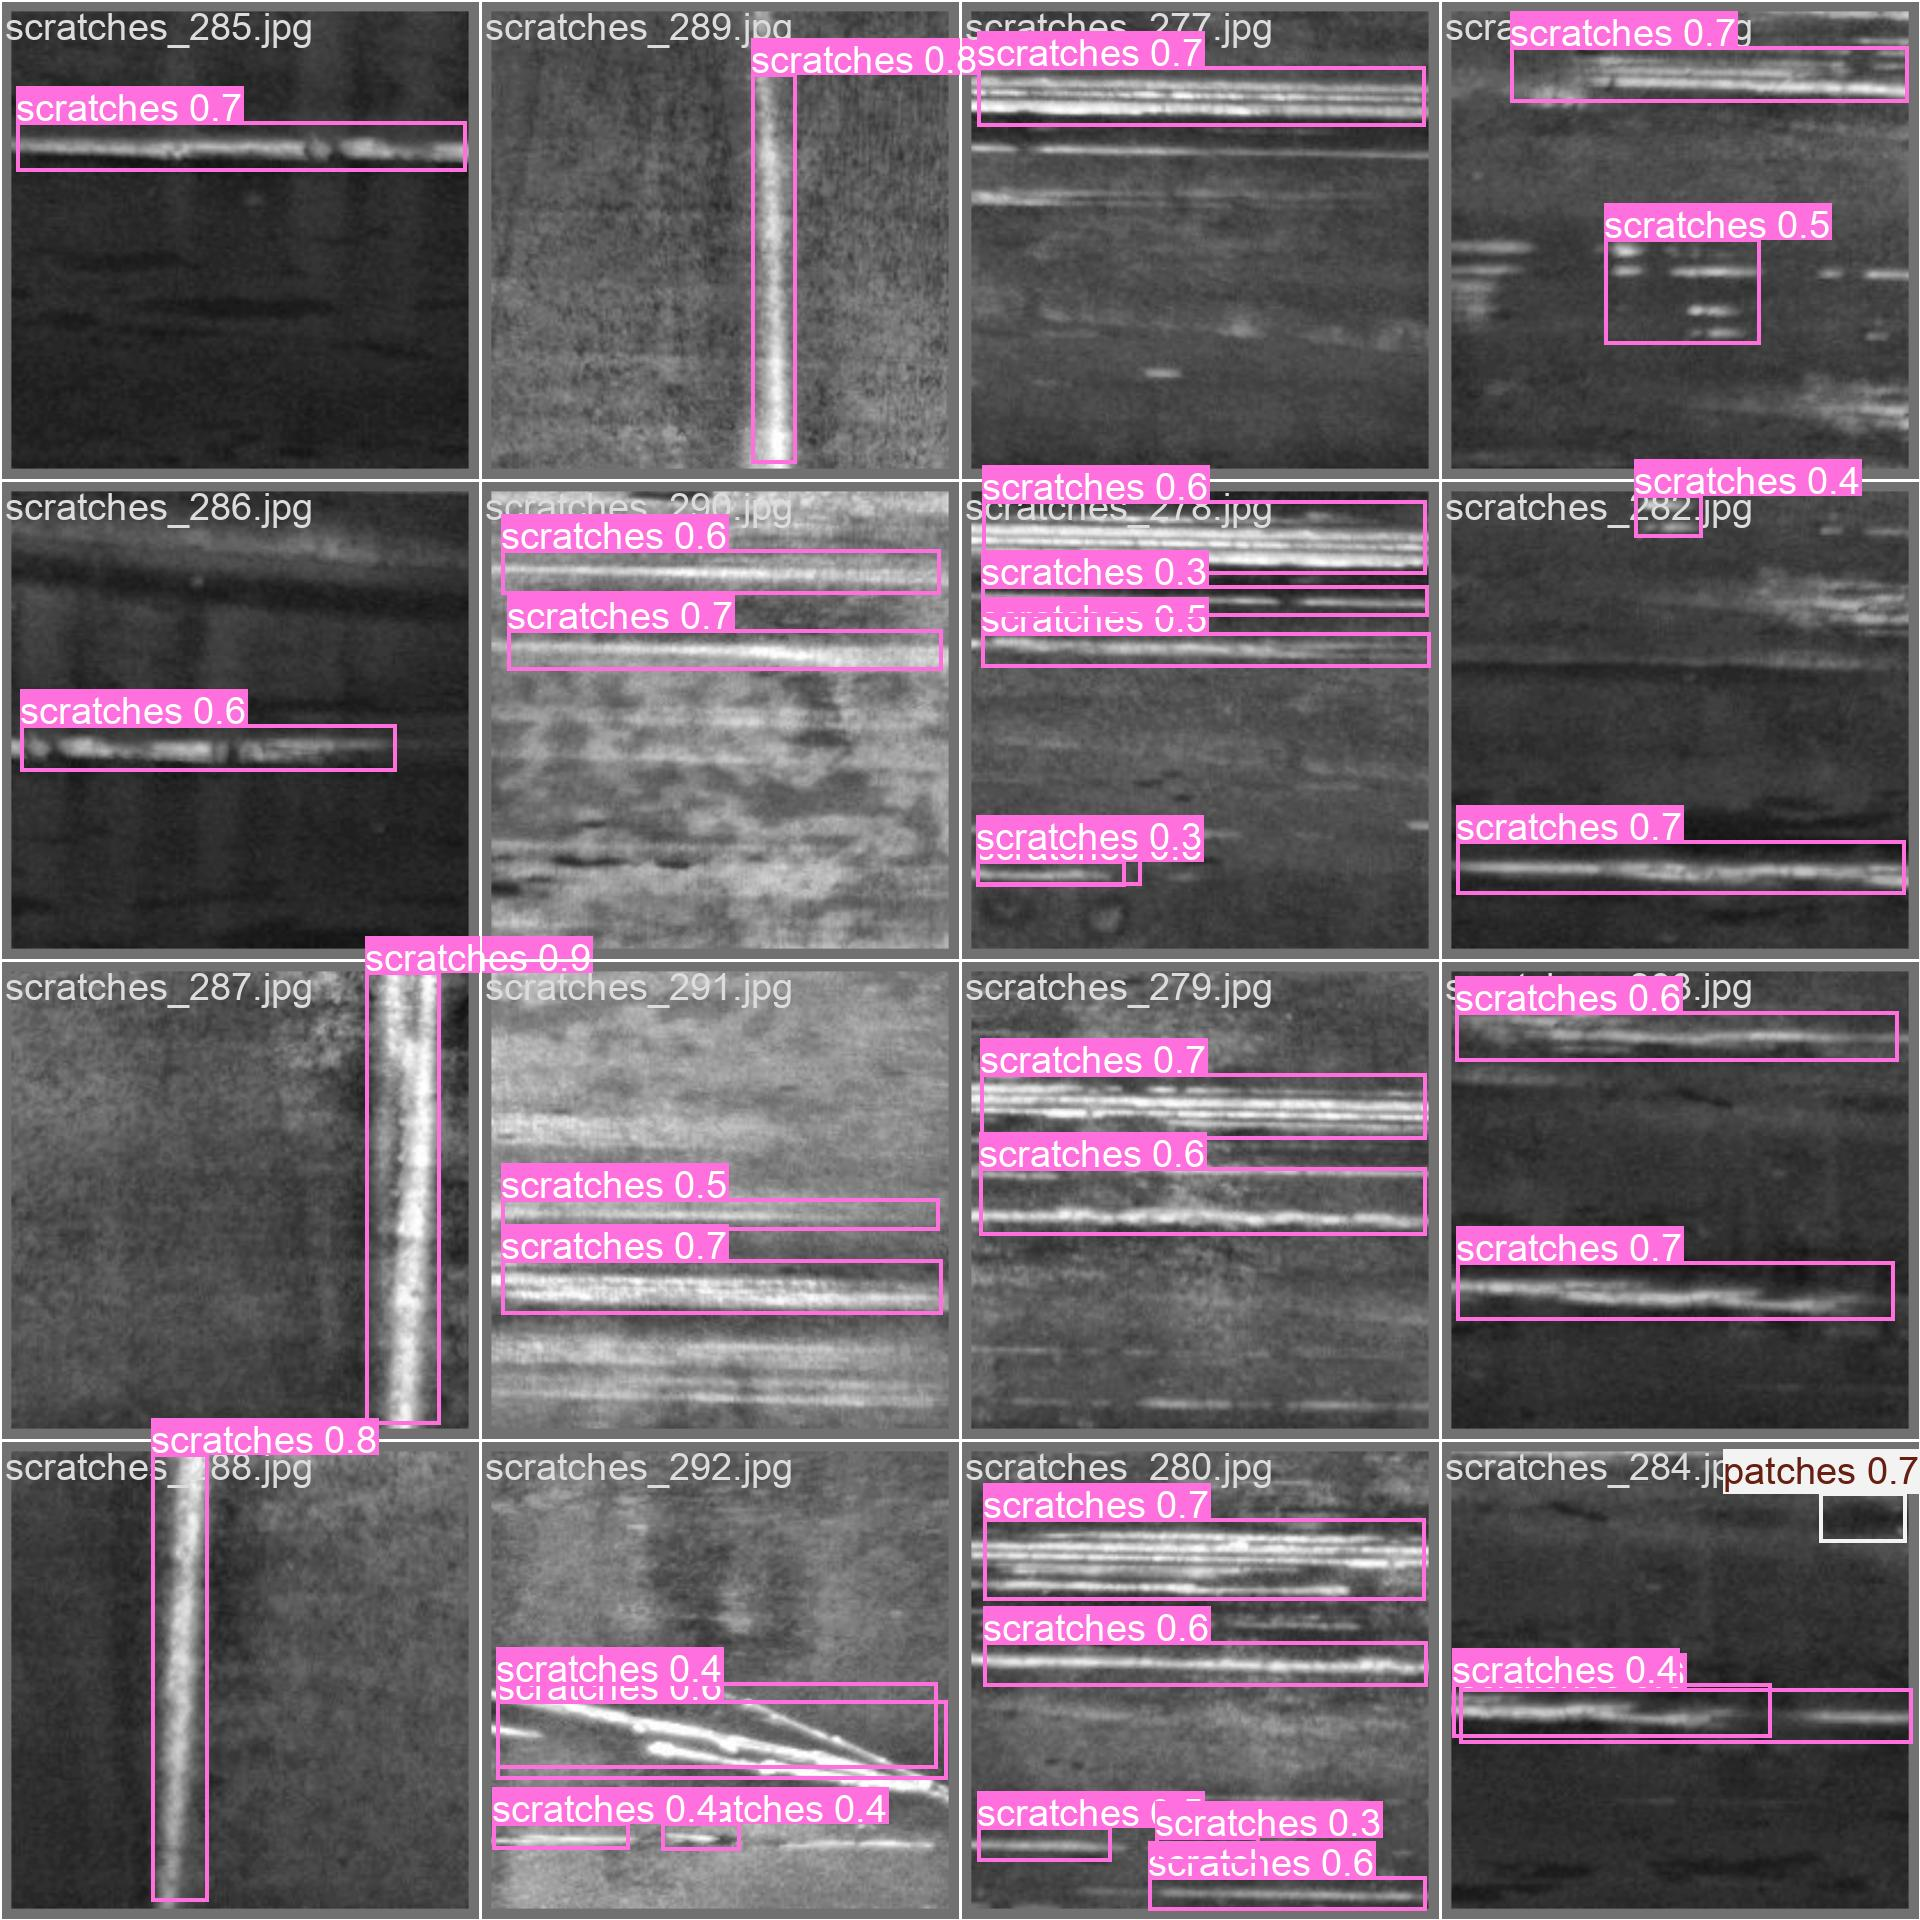
\includegraphics[width=0.2\linewidth]{img/val_batch0_predg.jpg}
		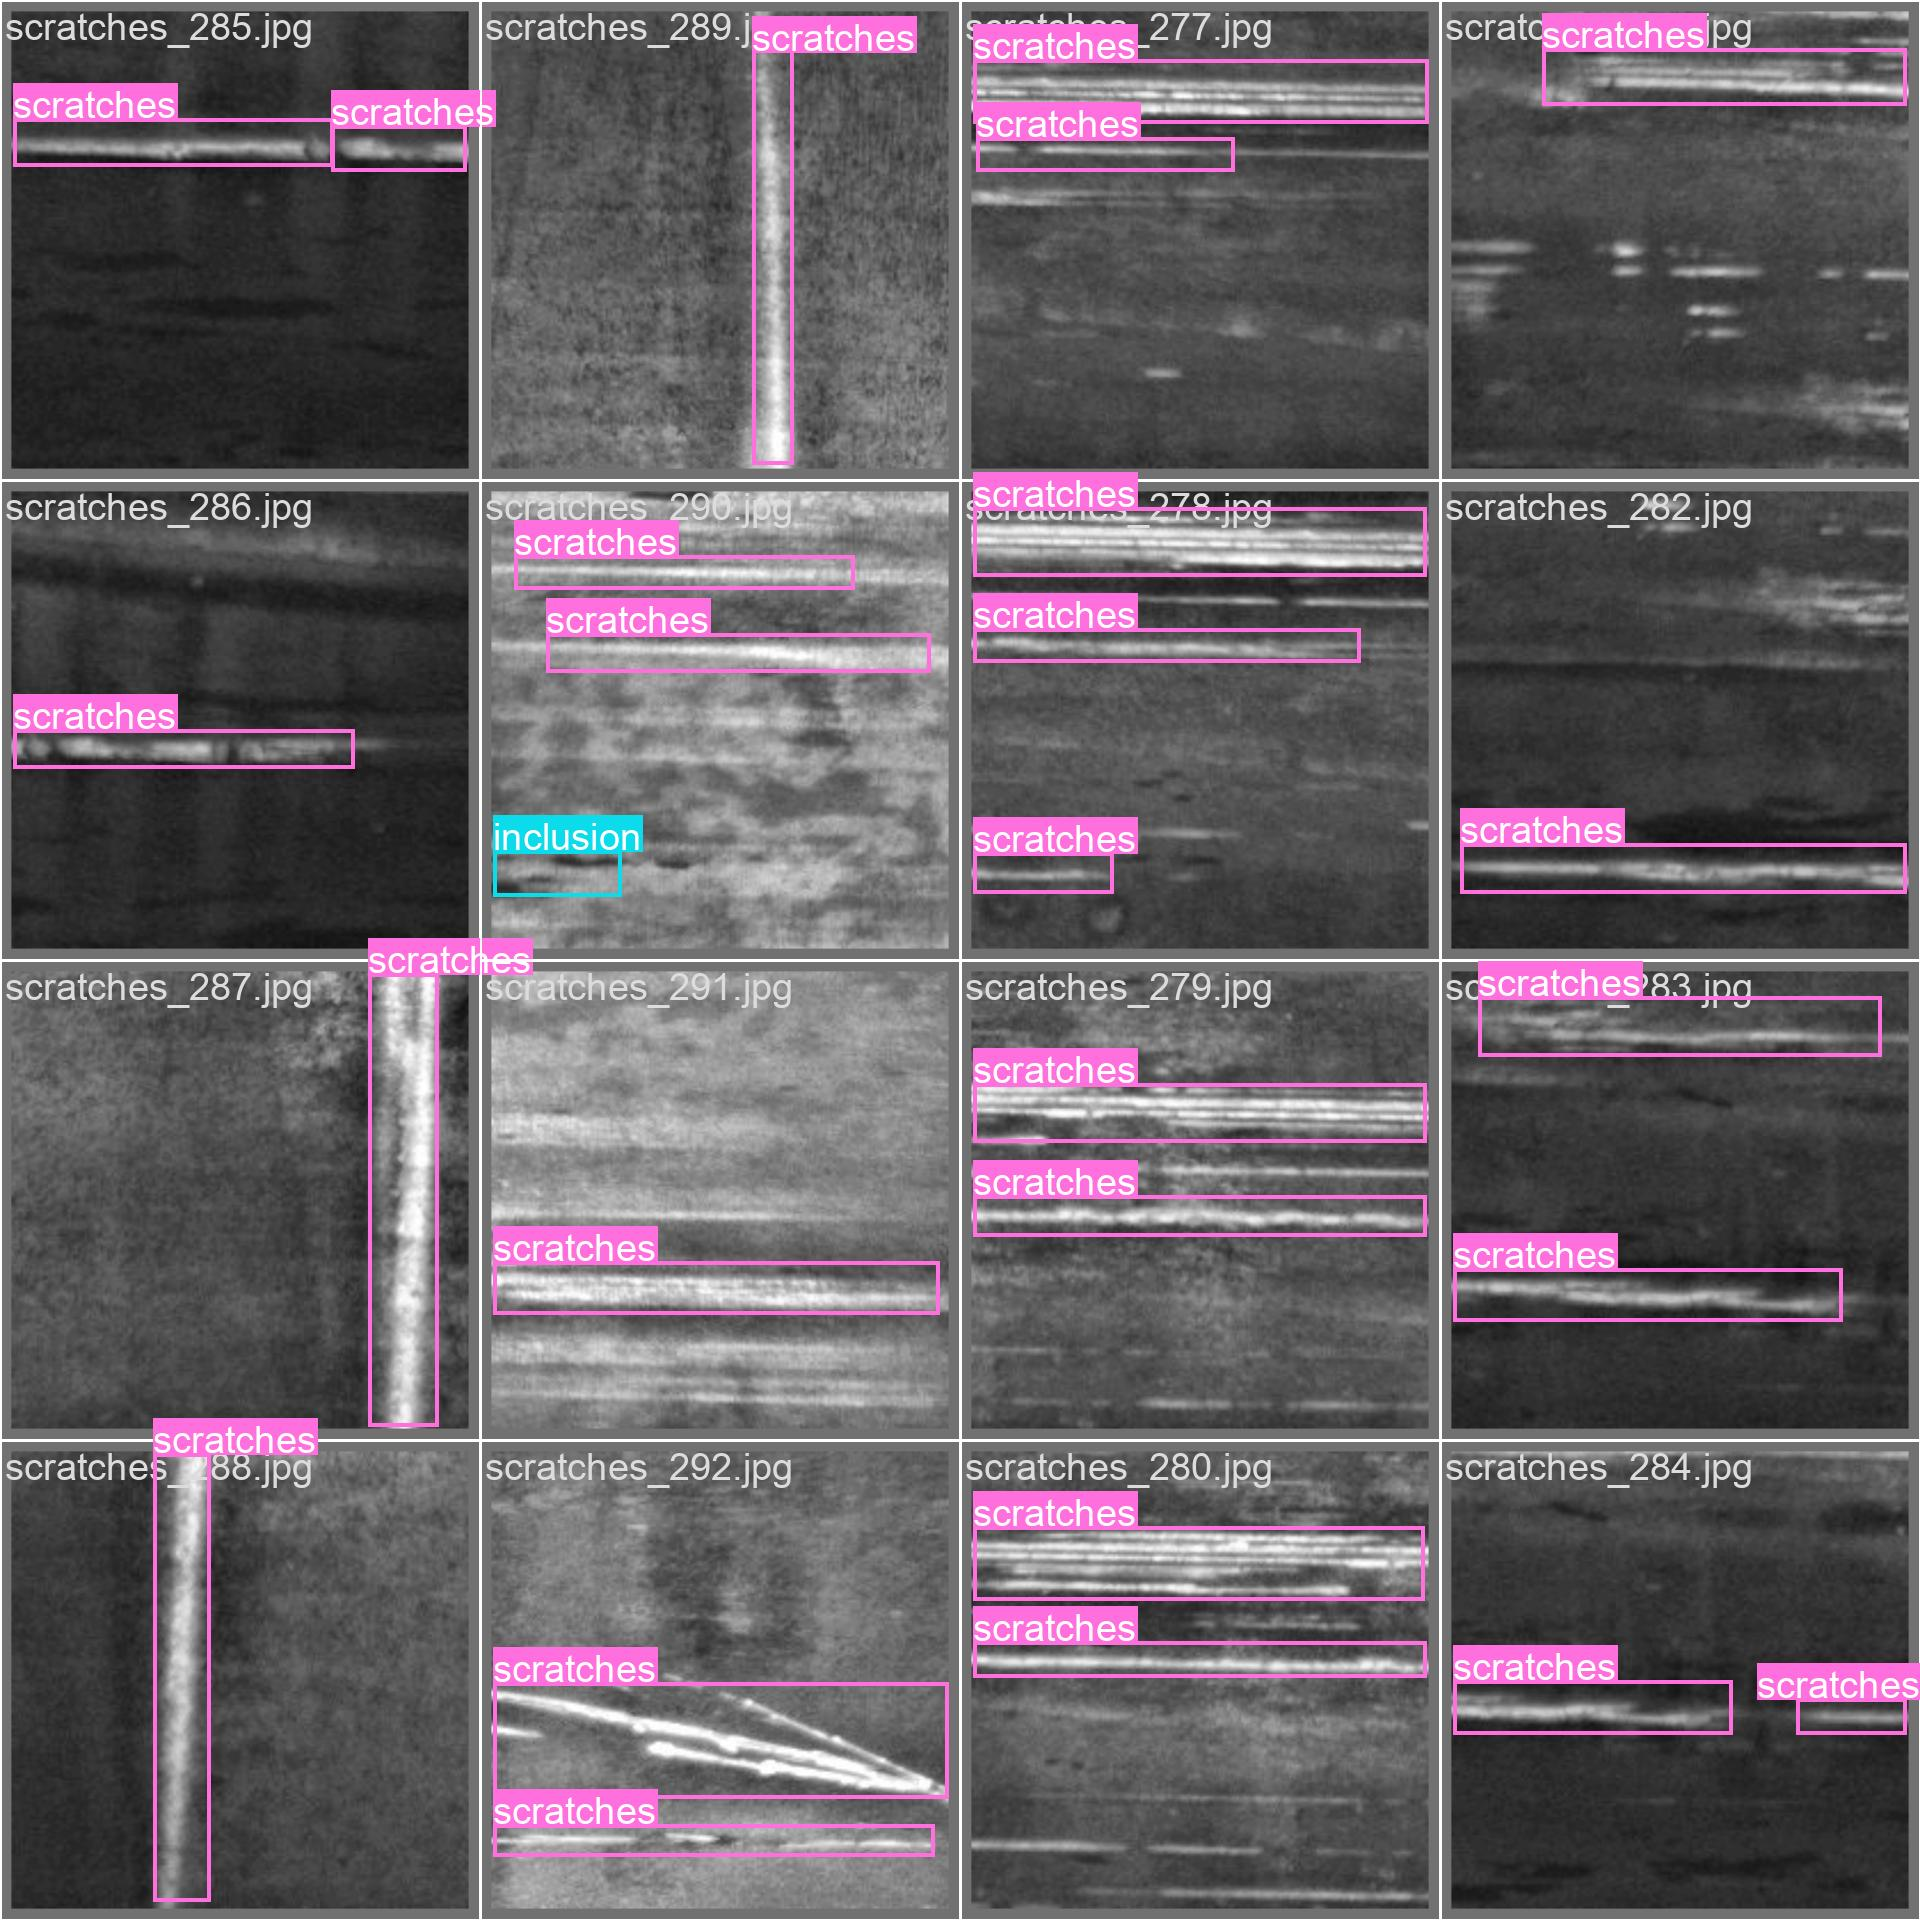
\includegraphics[width=0.2\linewidth]{img/val_batch0_labelsg.jpg}
		\caption{نمونه‌هایی از تشخیص مدل به همراه \lr{ground truth} آن(سمت راست لیبل ها و سمت چپ پیش بینی)}
	\end{figure}
	
	همانطور که مشاهده می‌شود از نمونه‌ها هم معلوم است که مدل در تشخیص پس‌زمینه عملکرد مناسبی ندارد و بیشتر در آنجا دچار خطا می‌شود.
	
	\subsection{پیاده‌سازی مدل \lr{YOLOV8n-Improvement}}
	\begin{figure}[H]
		\centering
		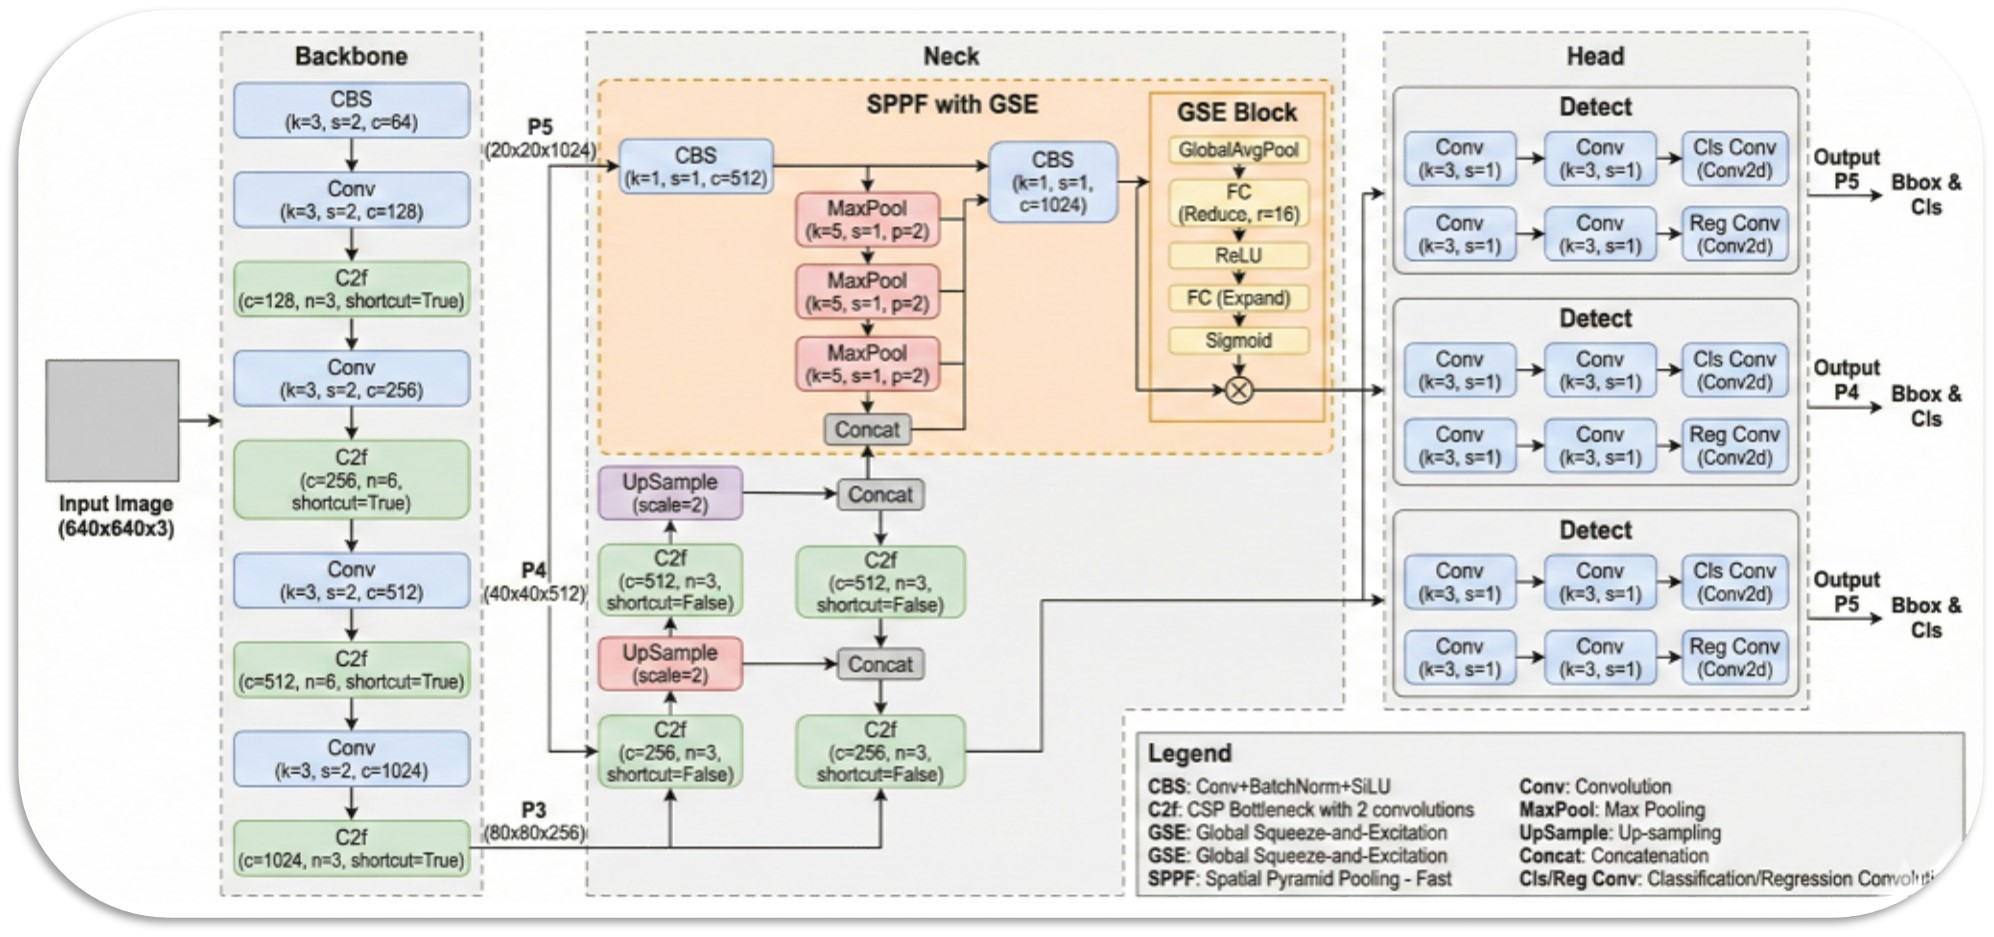
\includegraphics[width=0.8\linewidth]{img/yolov8-improvement.jpg}
		\caption{ساختار مدل \lr{yolov8n-Improvement} (تصویر ساخته شده با هوش مصنوعی)}
	\end{figure}
	در این پروژه، نسخه‌ای بهبودیافته و سبک از مدل YOLOv8n با عنوان YOLOv8n-improvement ارائه شده است. این معماری با اعمال تغییرات ساختاری و بهینه‌سازی در سطوح مختلف شبکه، شامل ماژول استخراج ویژگی \lr{CSP-ABAN}، مکانیزم توجه سراسری \lr{GAM}، ماژول کانولوشن \lr{GSConv}، تابع هزینه \lr{PIoUv2} و همچنین بلوک توجه \lr{GSE} بهبودیافته در ماژول \lr{SPPF} طراحی شده است.
	
	ترکیب این اجزا یک ساختار هم‌افزا (\lr{Synergistic}) از مرحله استخراج ویژگی تا بهینه‌سازی نهایی ایجاد می‌کند که منجر به افزایش دقت و پایداری مدل در عین حفظ سبکی آن می‌شود.
	
	%--------------------------------------------------
	
	\subsection{معماری کلی شبکه}
	
	در مدل YOLOv8n-Improvement تغییرات زیر نسبت به YOLOv8n پایه اعمال شده است:
	
	\begin{itemize}
		\item جایگزینی کانولوشن‌های استاندارد با GSConv در بخش‌های کلیدی Backbone و Neck
		\item بازطراحی ماژول‌های C2f به صورت CSP-ABAN
		\item ادغام مکانیزم توجه سراسری GAM
		\item جایگزینی تابع هزینه CIoU با PIoUv2
		\item افزودن بلوک توجه GSE بهبودیافته در SPPF
	\end{itemize}
	
	این تغییرات به صورت یک ساختار انتها به انتها (End-to-End) عمل کرده و جریان ویژگی و گرادیان را به شکل هماهنگ بهینه می‌کنند.
	
	%--------------------------------------------------
	
	\subsection{ماژول استخراج ویژگی CSP-ABAN}
	
	ماژول C2f در YOLOv8 اگرچه قدرت استخراج ویژگی بالایی دارد، اما باعث افزایش پیچیدگی محاسباتی می‌شود. به همین منظور، ماژول CSP-ABAN طراحی شده است که ترکیبی از ساختار CSPNet و کانولوشن دو مسیره (DualConv) می‌باشد.
	
	هر بلوک DualConv شامل:
	
	\begin{itemize}
		\item کانولوشن گروهی $3 \times 3$ با 4 گروه
		\item کانولوشن $1 \times 1$ برای فشرده‌سازی کانالی
	\end{itemize}
	
	کانولوشن گروهی موجب استخراج کارآمد اطلاعات فضایی شده و کانولوشن $1 \times 1$ تبادل اطلاعات بین کانال‌ها را تسهیل می‌کند. همچنین ساختار CSP از محاسبات تکراری جلوگیری کرده و کارایی شبکه را افزایش می‌دهد.
	
	این طراحی تعادل مناسبی بین توان بازنمایی ویژگی و هزینه محاسباتی برقرار می‌کند.
	
	%--------------------------------------------------
	
	\subsection{مکانیزم توجه سراسری (GAM)}
	
	برای افزایش توان تمایز ویژگی‌ها، مکانیزم توجه سراسری GAM به مدل افزوده شده است.
	
	برای نگاشت ورودی $F_1$، ابتدا توجه کانالی اعمال می‌شود:
	
	\begin{equation}
		F_2 = F_1 \cdot \sigma(\text{ChannelAttention}(F_1))
	\end{equation}
	
	سپس توجه فضایی اعمال می‌شود:
	
	\begin{equation}
		F_3 = F_2 \cdot \sigma(\text{SpatialAttention}(F_2))
	\end{equation}
	
	که در آن $\sigma$ تابع سیگموید است.
	
	زیرماژول توجه کانالی از یک ساختار MLP دو لایه با نسبت فشرده‌سازی $r$ استفاده می‌کند. زیرماژول توجه فضایی نیز شامل دو لایه کانولوشن بدون استفاده از Max-Pooling است تا از اتلاف اطلاعات جلوگیری شود.
	
	این مکانیزم موجب سرکوب نواحی غیرمهم و تقویت نواحی حاوی ویژگی‌های هدف می‌شود.
	
	%--------------------------------------------------
	
	\subsection{ماژول کانولوشن GSConv}
	
	به منظور حفظ سبکی مدل همراه با افزایش تبادل اطلاعات کانالی، کانولوشن‌های استاندارد با GSConv جایگزین شده‌اند.
	
	ساختار GSConv شامل:
	
	\begin{itemize}
		\item کانولوشن استاندارد
		\item کانولوشن عمقی تفکیک‌پذیر (\lr{Depthwise Separable})
		\item الحاق کانالی
		\item عملیات Channel Shuffle
	\end{itemize}
	
	ترکیب کانولوشن استاندارد و عمقی موجب افزایش توان استخراج ویژگی شده و عملیات Shuffle تبادل اطلاعات بین کانال‌ها را تقویت می‌کند. این ماژول نسبت به DWConv کارایی بازنمایی بالاتری ارائه می‌دهد.
	%------------------------------
	
	\subsection{بلوک توجه GSE بهبودیافته در SPPF}
	
	برای تقویت بازتنظیم کانالی ویژگی‌ها، یک بلوک GSE بهبودیافته در خروجی SPPF افزوده شده است.
	
	مقیاس توجه به صورت زیر محاسبه می‌شود:
	
	\begin{equation}
		S = \sigma(\text{MLP}(\text{GAP}(X) + \text{GMP}(X)))
	\end{equation}
	
	\begin{equation}
		Y = X \cdot S
	\end{equation}
	
	در اینجا GAP و GMP به ترتیب بیانگر میانگین‌گیری و بیشینه‌گیری سراسری هستند.
	
	استفاده همزمان از این دو نوع Pooling موجب حفظ اطلاعات بحرانی و تقویت کانال‌های مهم می‌شود.
	
	%--------------------------------------------------
	
	\subsection{تابع هزینه PIoUv2}
	
	در YOLOv8 پایه از CIoU استفاده می‌شود. در این پروژه، تابع PIoUv2 جایگزین شده است.
	
	ابتدا عامل جریمه تطبیقی تعریف می‌شود:
	
	\begin{equation}
		P = \frac{1}{4} \left( \frac{dw_1}{w_{gt}} + \frac{dw_2}{w_{gt}} + \frac{dh_1}{h_{gt}} + \frac{dh_2}{h_{gt}} \right)
	\end{equation}
	
	\begin{equation}
		f(P) = 1 - e^{-P^2}
	\end{equation}
	
	\begin{equation}
		L_{PIoU} = 1 - IoU + f(P)
	\end{equation}
	
	در نسخه PIoUv2 یک تابع توجه غیر یکنواخت افزوده شده است:
	
	\begin{equation}
		q = e^{-P}
	\end{equation}
	
	\begin{equation}
		u(x) = 3x e^{-x^2}
	\end{equation}
	
	\begin{equation}
		L_{PIoUv2} = u(\lambda q) \cdot L_{PIoU}
	\end{equation}
	
	این تابع تمرکز بیشتری بر جعبه‌های با کیفیت متوسط ایجاد کرده و همگرایی سریع‌تری نسبت به CIoU فراهم می‌کند.
	
	%--------------------------------------------------
	
	\subsection{مکانیزم هم‌افزایی ماژول‌ها}
	
	در معماری \lr{YOLOv8n-Improvement}، ماژول‌ها به صورت زنجیره‌ای و هم‌افزا عمل می‌کنند:
	
	\begin{itemize}
		\item CSP-ABAN استخراج سلسله‌مراتبی و حذف افزونگی را انجام می‌دهد.
		\item GAM وزن‌دهی پویا در ابعاد فضایی و کانالی را اعمال می‌کند.
		\item PIoUv2 نظارت دقیق بر رگرسیون جعبه‌ها اعمال می‌کند.
	\end{itemize}
	
	این طراحی هماهنگ موجب بهبود دقت، افزایش پایداری آموزش و ارتقای قابلیت تعمیم‌پذیری مدل در سناریوهای پیچیده می‌شود، در حالی که سبکی مدل حفظ می‌گردد.
	
	این ساختار و این نحوۀ آموزش مدل از یک مقالۀ \lr{IEEE} استخراج شده است که در سال 2025 چاپ گردیده است.
	
	نتایج مربوط به آموزش این مدل به صورت زیر است:
	\begin{figure}[H]
		\centering
		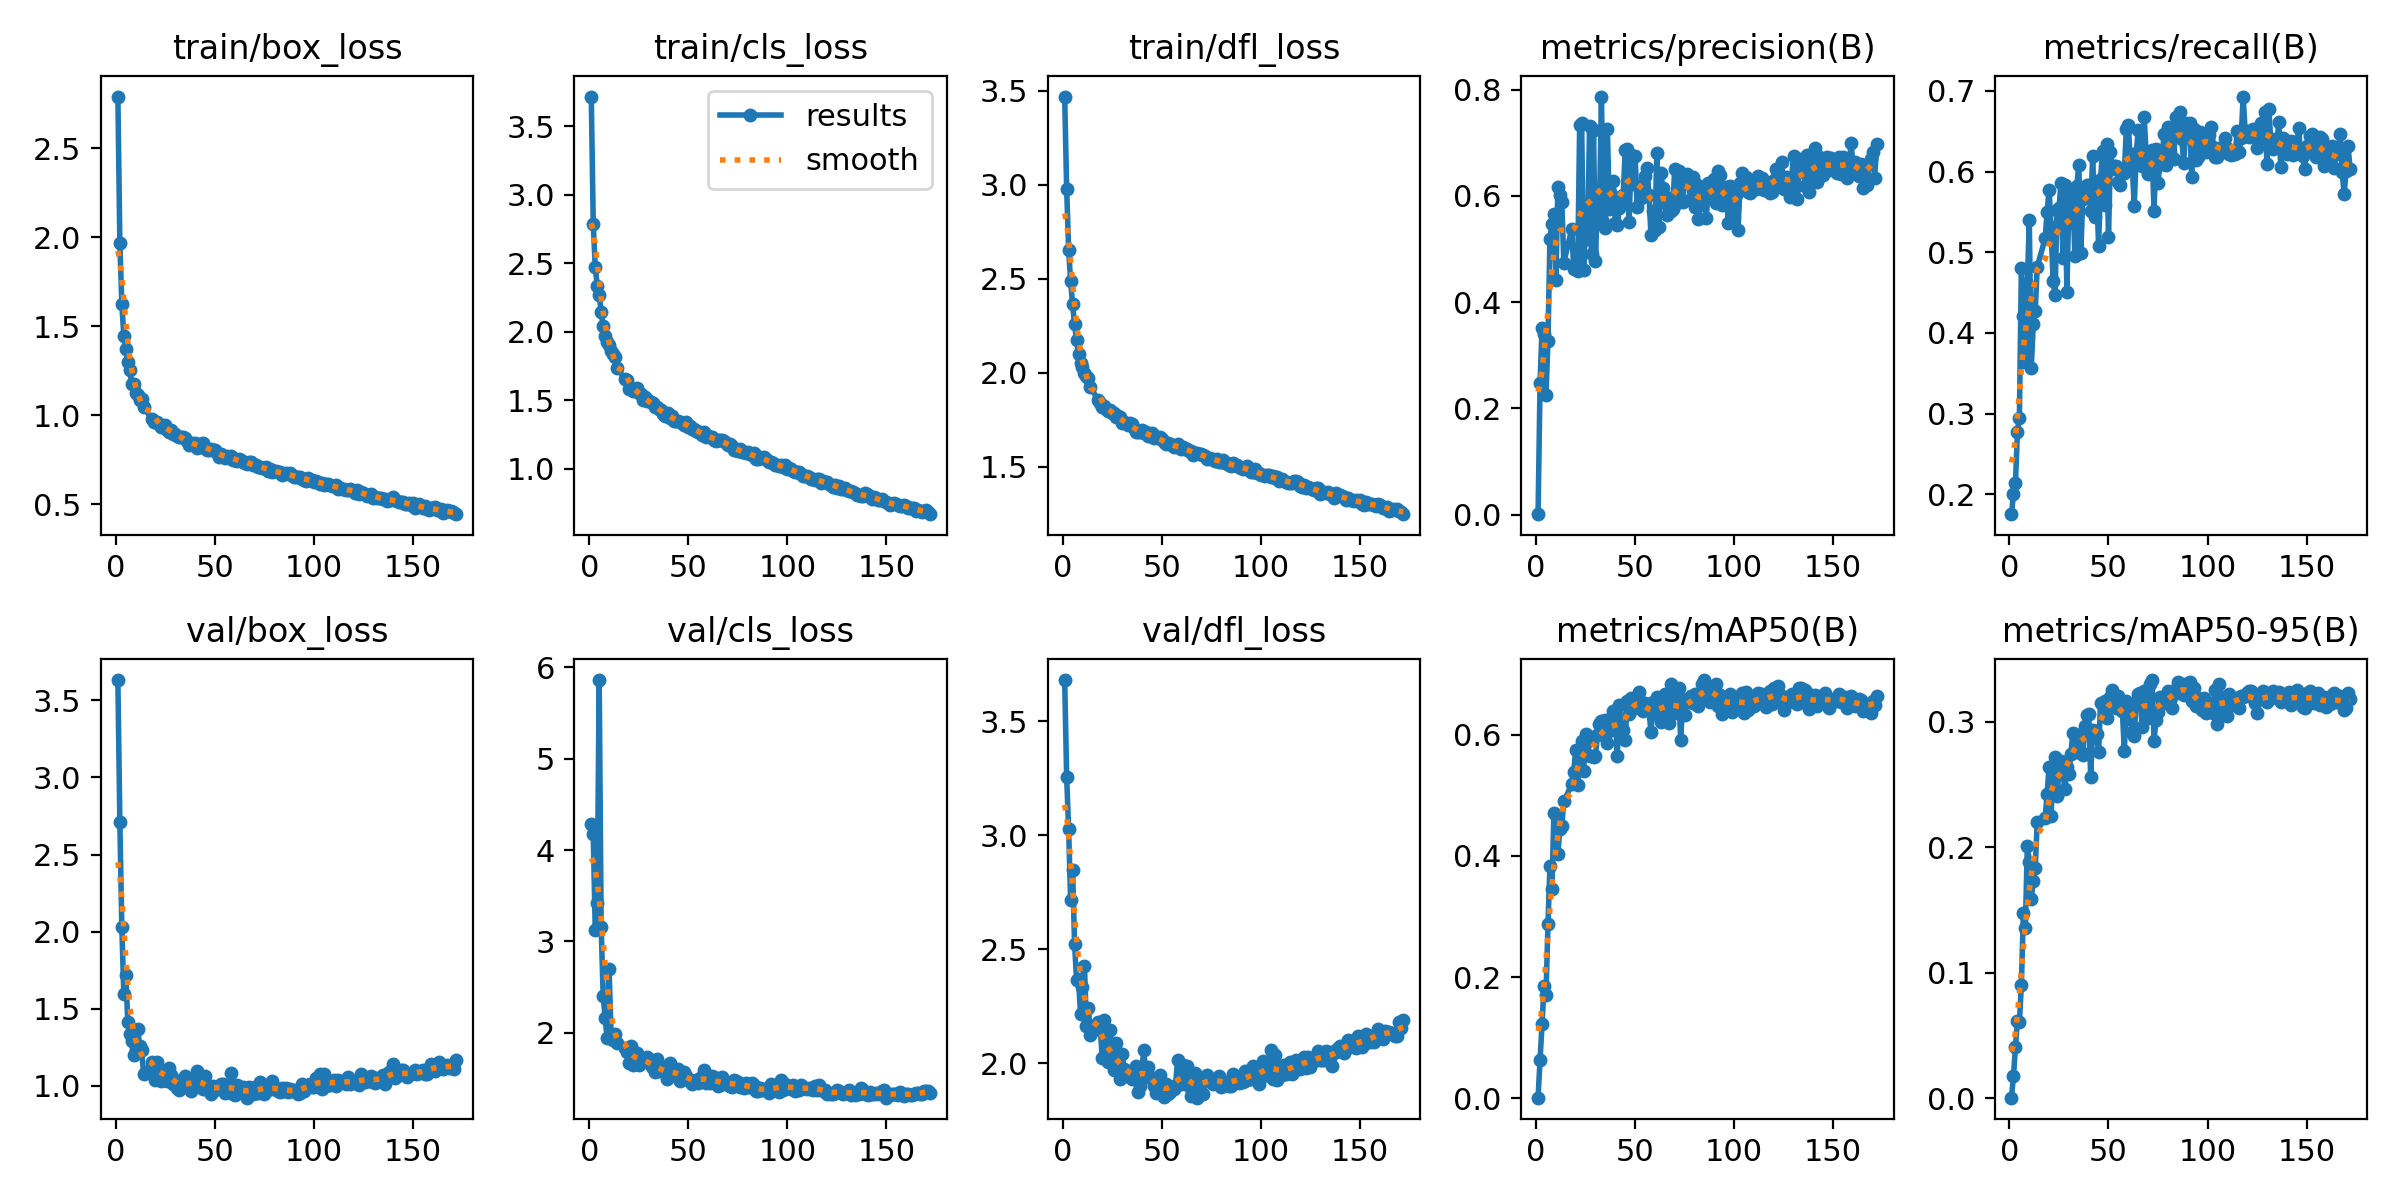
\includegraphics[width=0.9\linewidth]{img/resultsI.png}
		\caption{نمودارهای مربوط به روند آموزش مدل}
	\end{figure}
	همانطور که از نمودارها نیز مشخص است، مقدار ارور بر روی مجموعه دادۀ اعتبارسنجی کاهش یافته است و با اورفیتی که در مدل قبلی روبه رو بودیم، اینجا روبه رو نیستیم. مقدار \lr{Recall}، \lr{Precision} و \lr{mAP} تا حدودی بهبود یافته و یا تغییری نکرده است.
	
	
	
	\section{معیارهای ارزیابی عملکرد مدل}
	
	برای ارزیابی عملکرد مدل آشکارسازی اشیا از معیار میانگین دقت متوسط (\lr{Mean Average Precision - mAP}) استفاده می‌شود. این معیار یکی از استانداردترین شاخص‌ها در حوزه تشخیص اشیا بوده و عملکرد مدل را از نظر دقت طبقه‌بندی و کیفیت مکان‌یابی جعبه‌های مرزی به صورت هم‌زمان ارزیابی می‌کند.
	
	\subsection{Precision و Recall}
	
	ابتدا دو معیار پایه تعریف می‌شوند:
	
	\begin{equation}
		Precision = \frac{TP}{TP + FP}
	\end{equation}
	
	\begin{equation}
		Recall = \frac{TP}{TP + FN}
	\end{equation}
	
	که در آن:
	\begin{itemize}
		\item $TP$ تعداد نمونه‌های مثبت درست (\lr{True Positive})
		\item $FP$ تعداد نمونه‌های مثبت نادرست (\lr{False Positive})
		\item $FN$ تعداد نمونه‌های منفی نادرست (\lr{False Negative})
	\end{itemize}
	
	Precision میزان صحت پیش‌بینی‌های مثبت مدل و Recall میزان توانایی مدل در بازیابی تمامی نمونه‌های واقعی را اندازه‌گیری می‌کند.
	
	\subsection{Average Precision (AP)}
	
	برای هر کلاس، با تغییر آستانه اطمینان (\lr{Confidence Threshold})، منحنی \lr{Precision-Recall} ترسیم می‌شود. مساحت زیر این منحنی، معیار \lr{Average Precision (AP)} را تشکیل می‌دهد:
	
	\begin{equation}
		AP = \int_0^1 Precision(Recall) \, d(Recall)
	\end{equation}
	
	این مقدار بیانگر عملکرد مدل در یک کلاس مشخص است.
	
	\subsection{\lr{Mean Average Precision (mAP)}}
	
	میانگین AP در تمام کلاس‌ها به صورت زیر تعریف می‌شود:
	
	\begin{equation}
		mAP = \frac{1}{C} \sum_{i=1}^{C} AP_i
	\end{equation}
	
	که در آن $C$ تعداد کلاس‌ها است.
	
	\subsection{معیار \lr{mAP@0.5 (mAP50)}}
	
	در آشکارسازی اشیا، برای تعیین صحیح بودن یک پیش‌بینی از معیار همپوشانی \lr{IoU (Intersection over Union)} استفاده می‌شود:
	
	\begin{equation}
		IoU = \frac{Area_{intersection}}{Area_{union}}
	\end{equation}
	
	در معیار \lr{mAP@0.5}، یک پیش‌بینی زمانی صحیح در نظر گرفته می‌شود که:
	
	\begin{equation}
		IoU \geq 0.5
	\end{equation}
	
	به عبارت دیگر، اگر همپوشانی بین جعبه پیش‌بینی‌شده و جعبه واقعی حداقل 50 درصد باشد، آن پیش‌بینی به عنوان \lr{True Positive} محسوب می‌شود.
	
	
	
	
	\subsection{تفاوت \lr{mAP} و \lr{mAP50}}
	
	\begin{itemize}
		\item \lr{mAP50} تنها در آستانه \lr{IoU} برابر با \lr{0.5} محاسبه می‌شود.
		\item در نسخه‌های جدید \lr{YOLO}، معیار \lr{mAP@0.5:0.95} نیز گزارش می‌شود که میانگین \lr{mAP} در بازه آستانه‌های \lr{IoU} از \lr{0.5} تا \lr{0.95} با گام \lr{0.05} است.
	\end{itemize}
	
	معیار \lr{mAP@0.5} معمولاً مقدار بالاتری دارد و نشان‌دهنده توانایی کلی مدل در تشخیص اهداف است، در حالی که \lr{mAP@0.5:0.95} معیار سخت‌گیرانه‌تری بوده و کیفیت دقیق مکان‌یابی جعبه‌های مرزی را بهتر ارزیابی می‌کند.
	
	
	\begin{figure}[H]
		\centering
		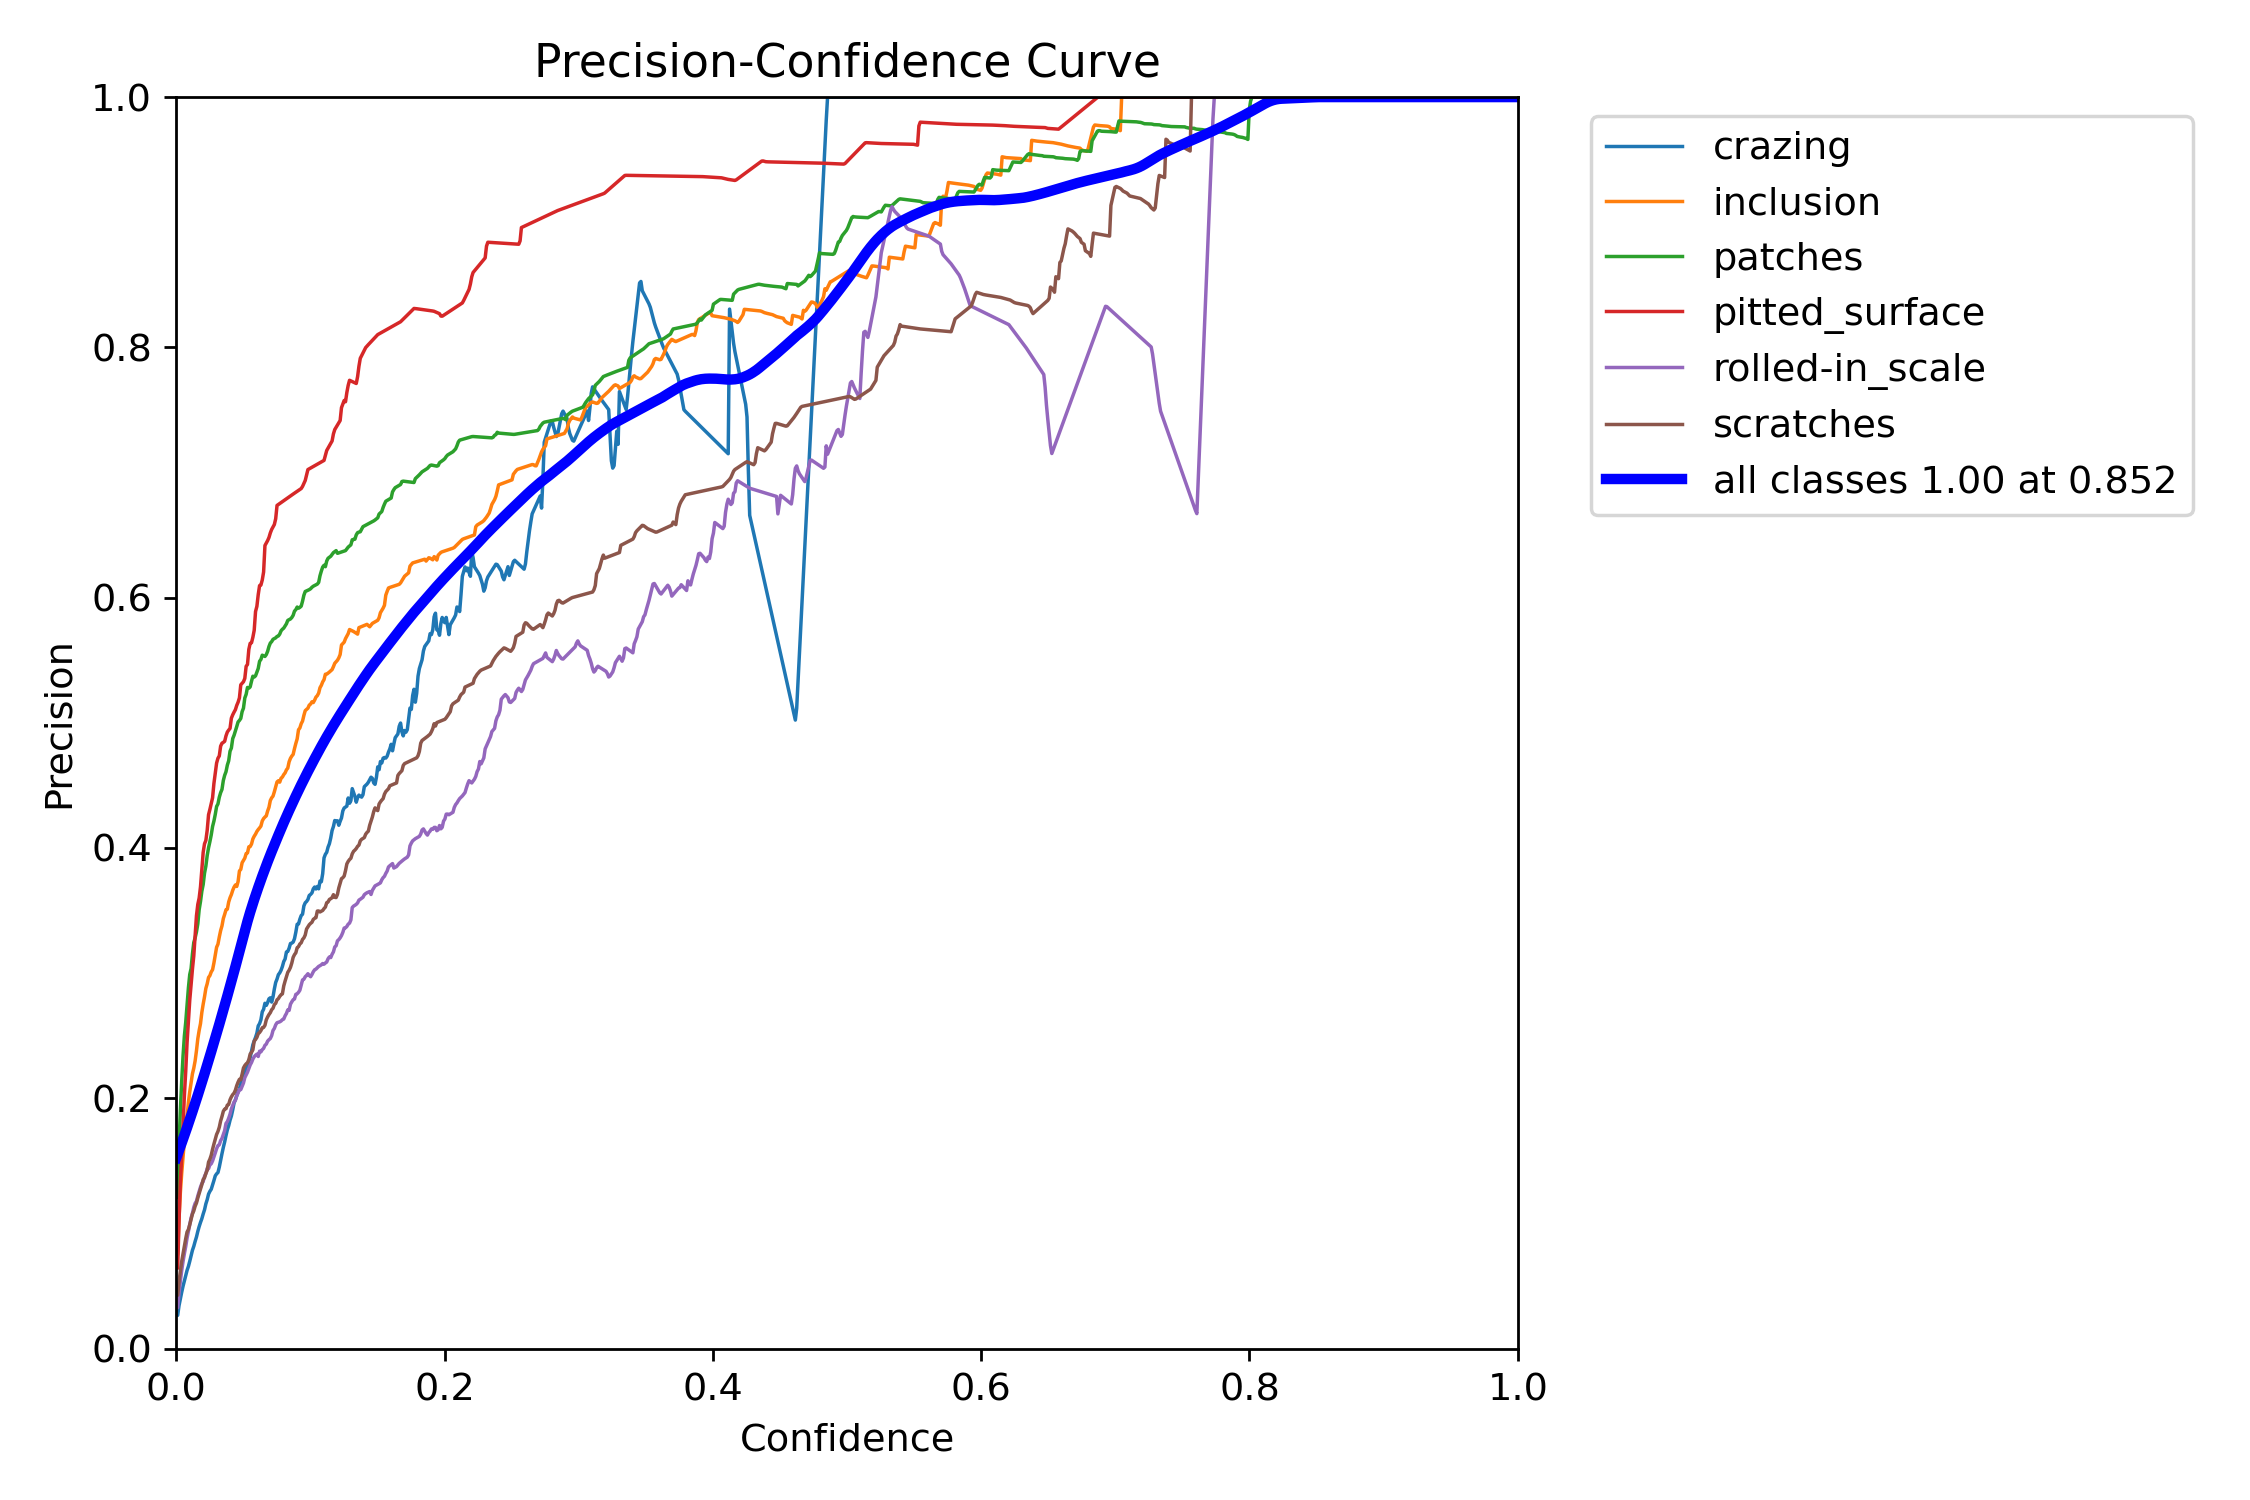
\includegraphics[width=0.45\linewidth]{img/BoxP_curveI.png}
		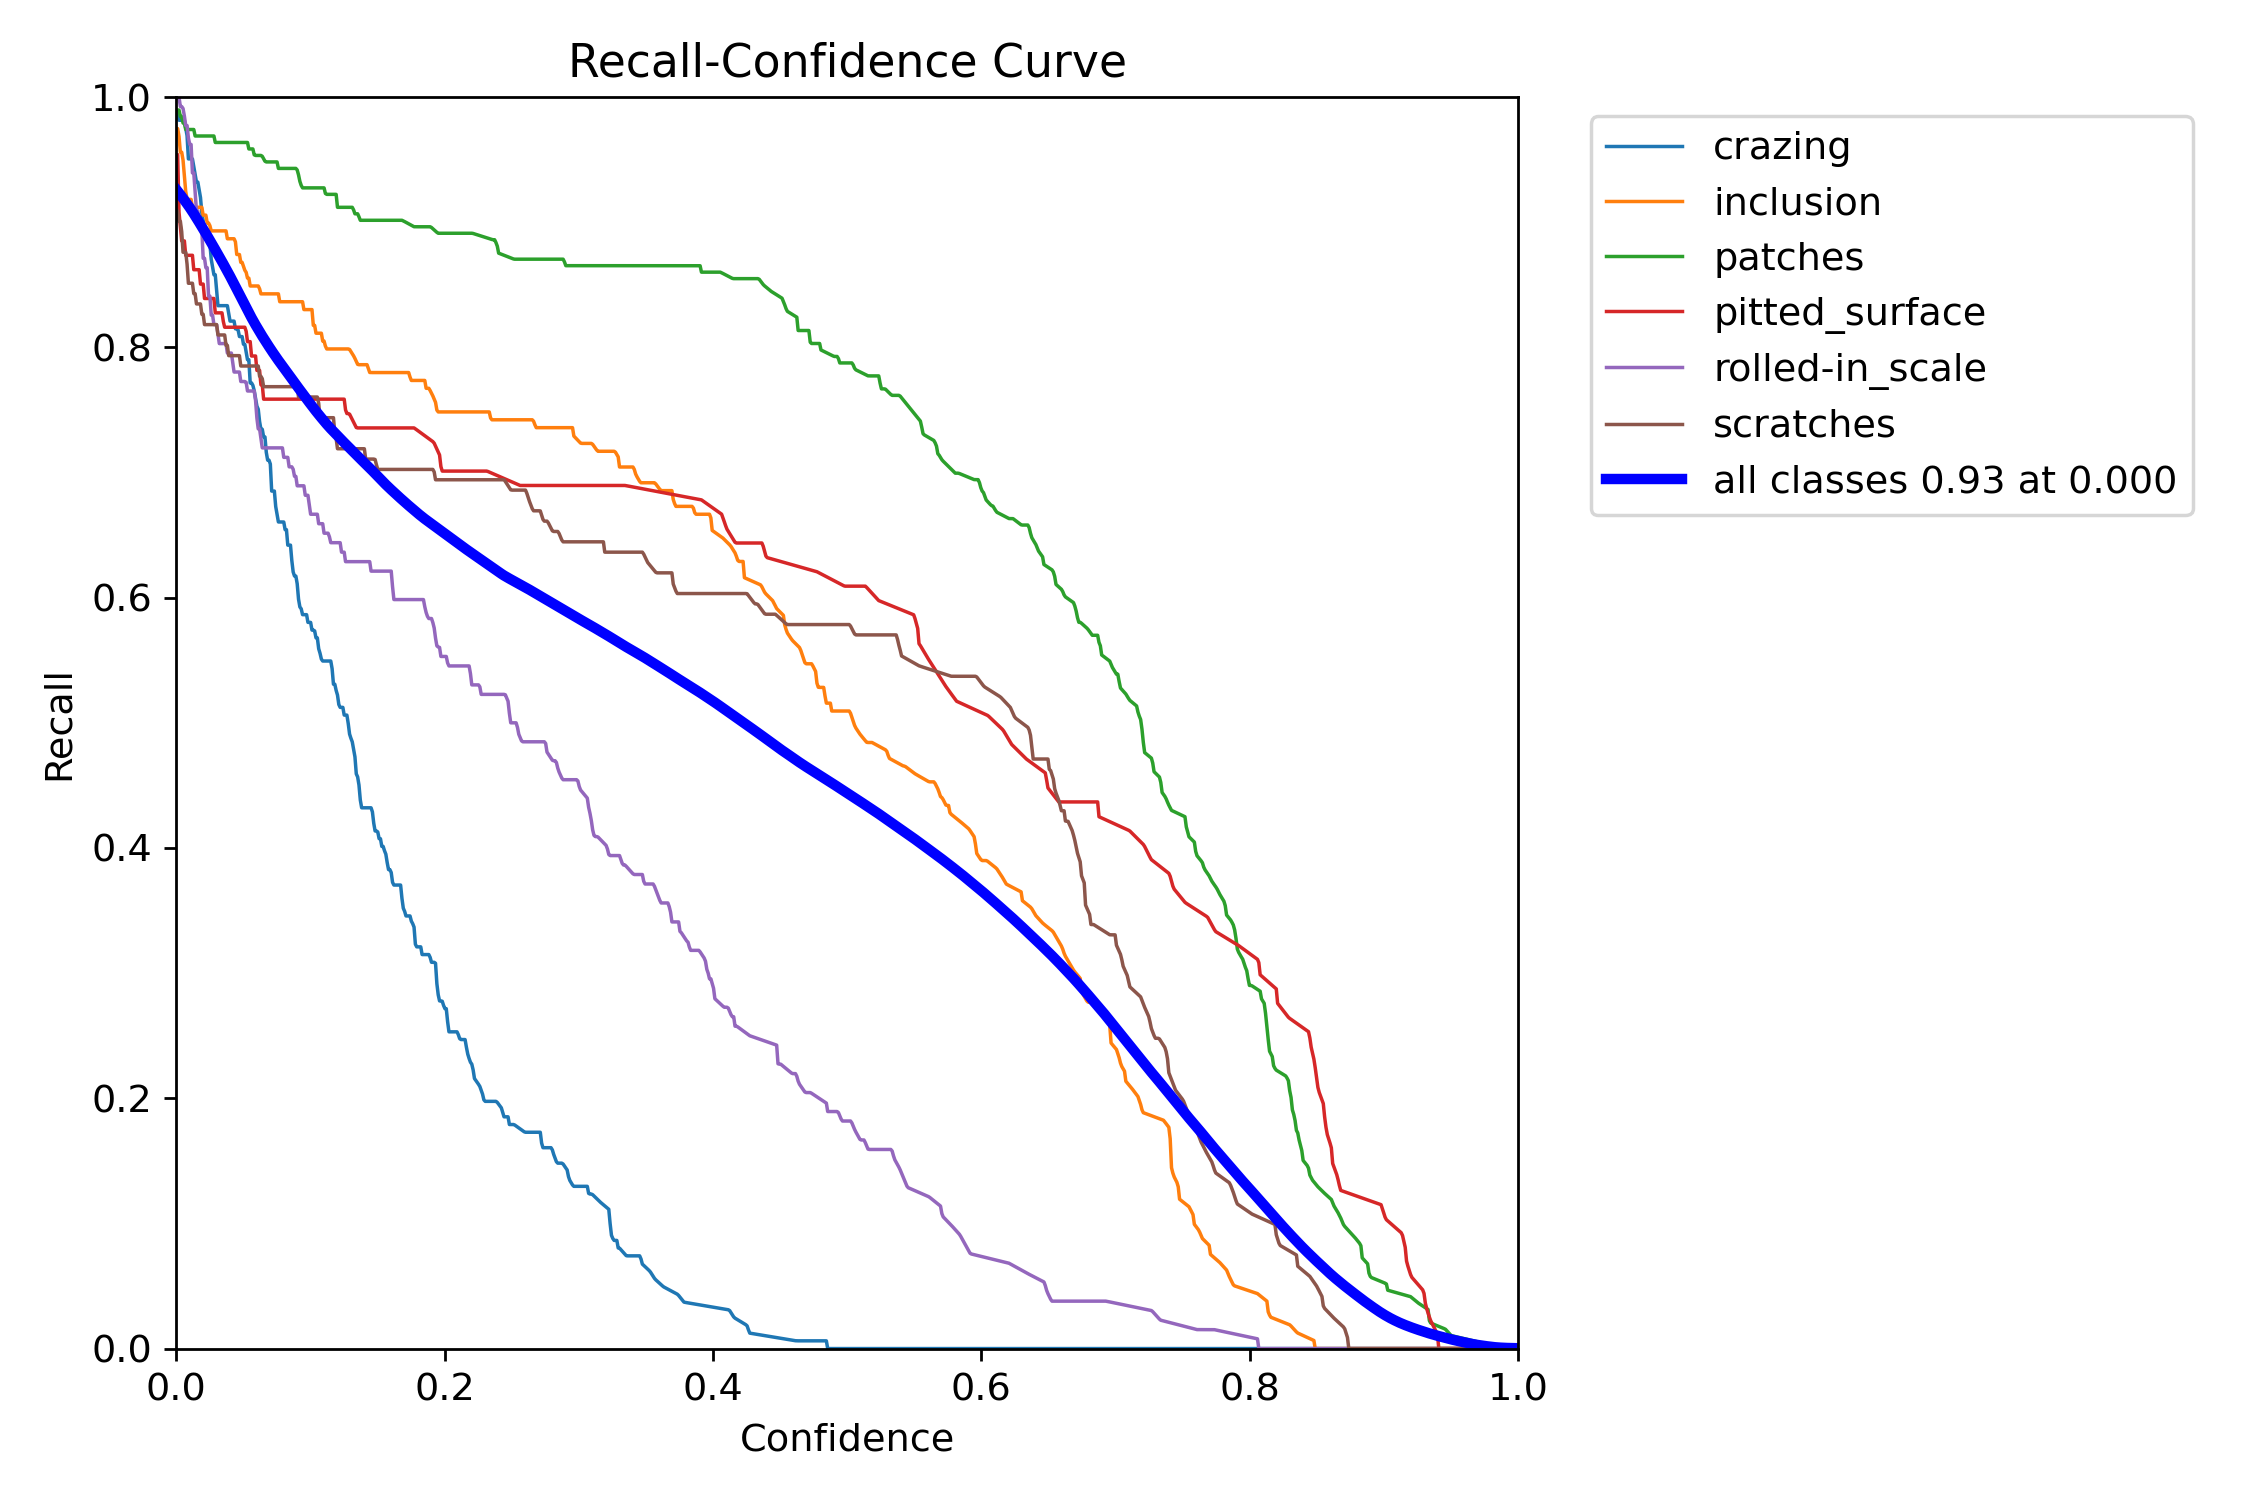
\includegraphics[width=0.45\linewidth]{img/BoxR_curveI.png}
		
		\vspace{0.3cm}
		
		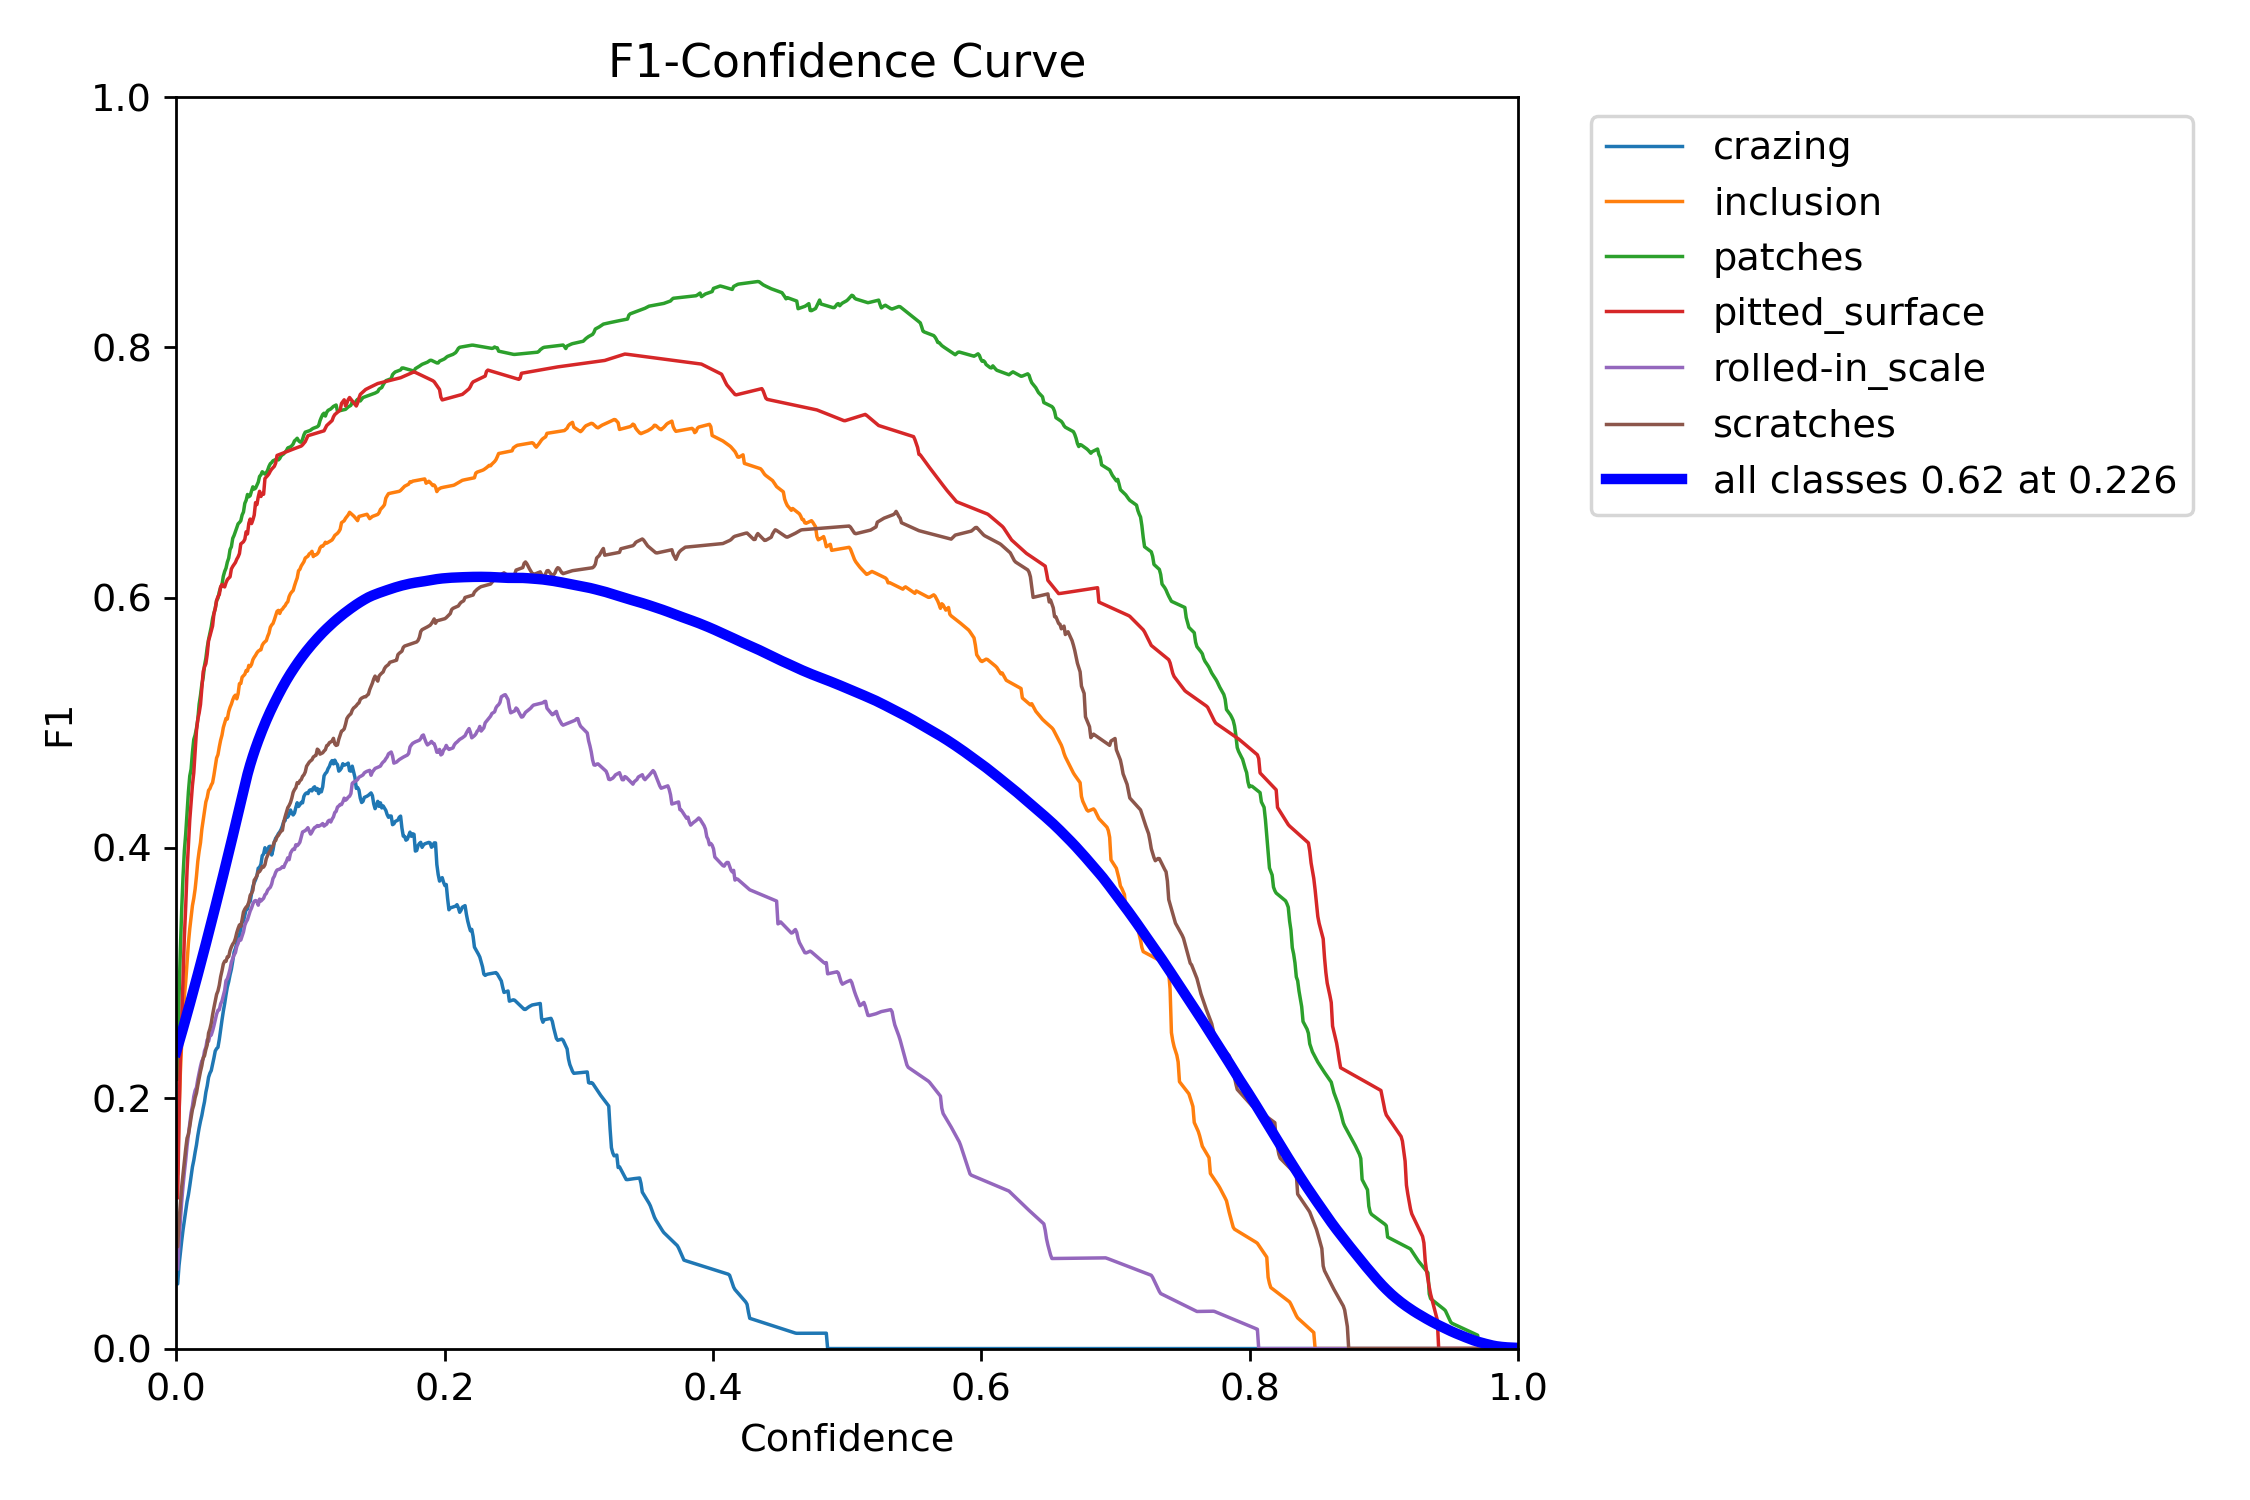
\includegraphics[width=0.45\linewidth]{img/BoxF1_curveI.png}
		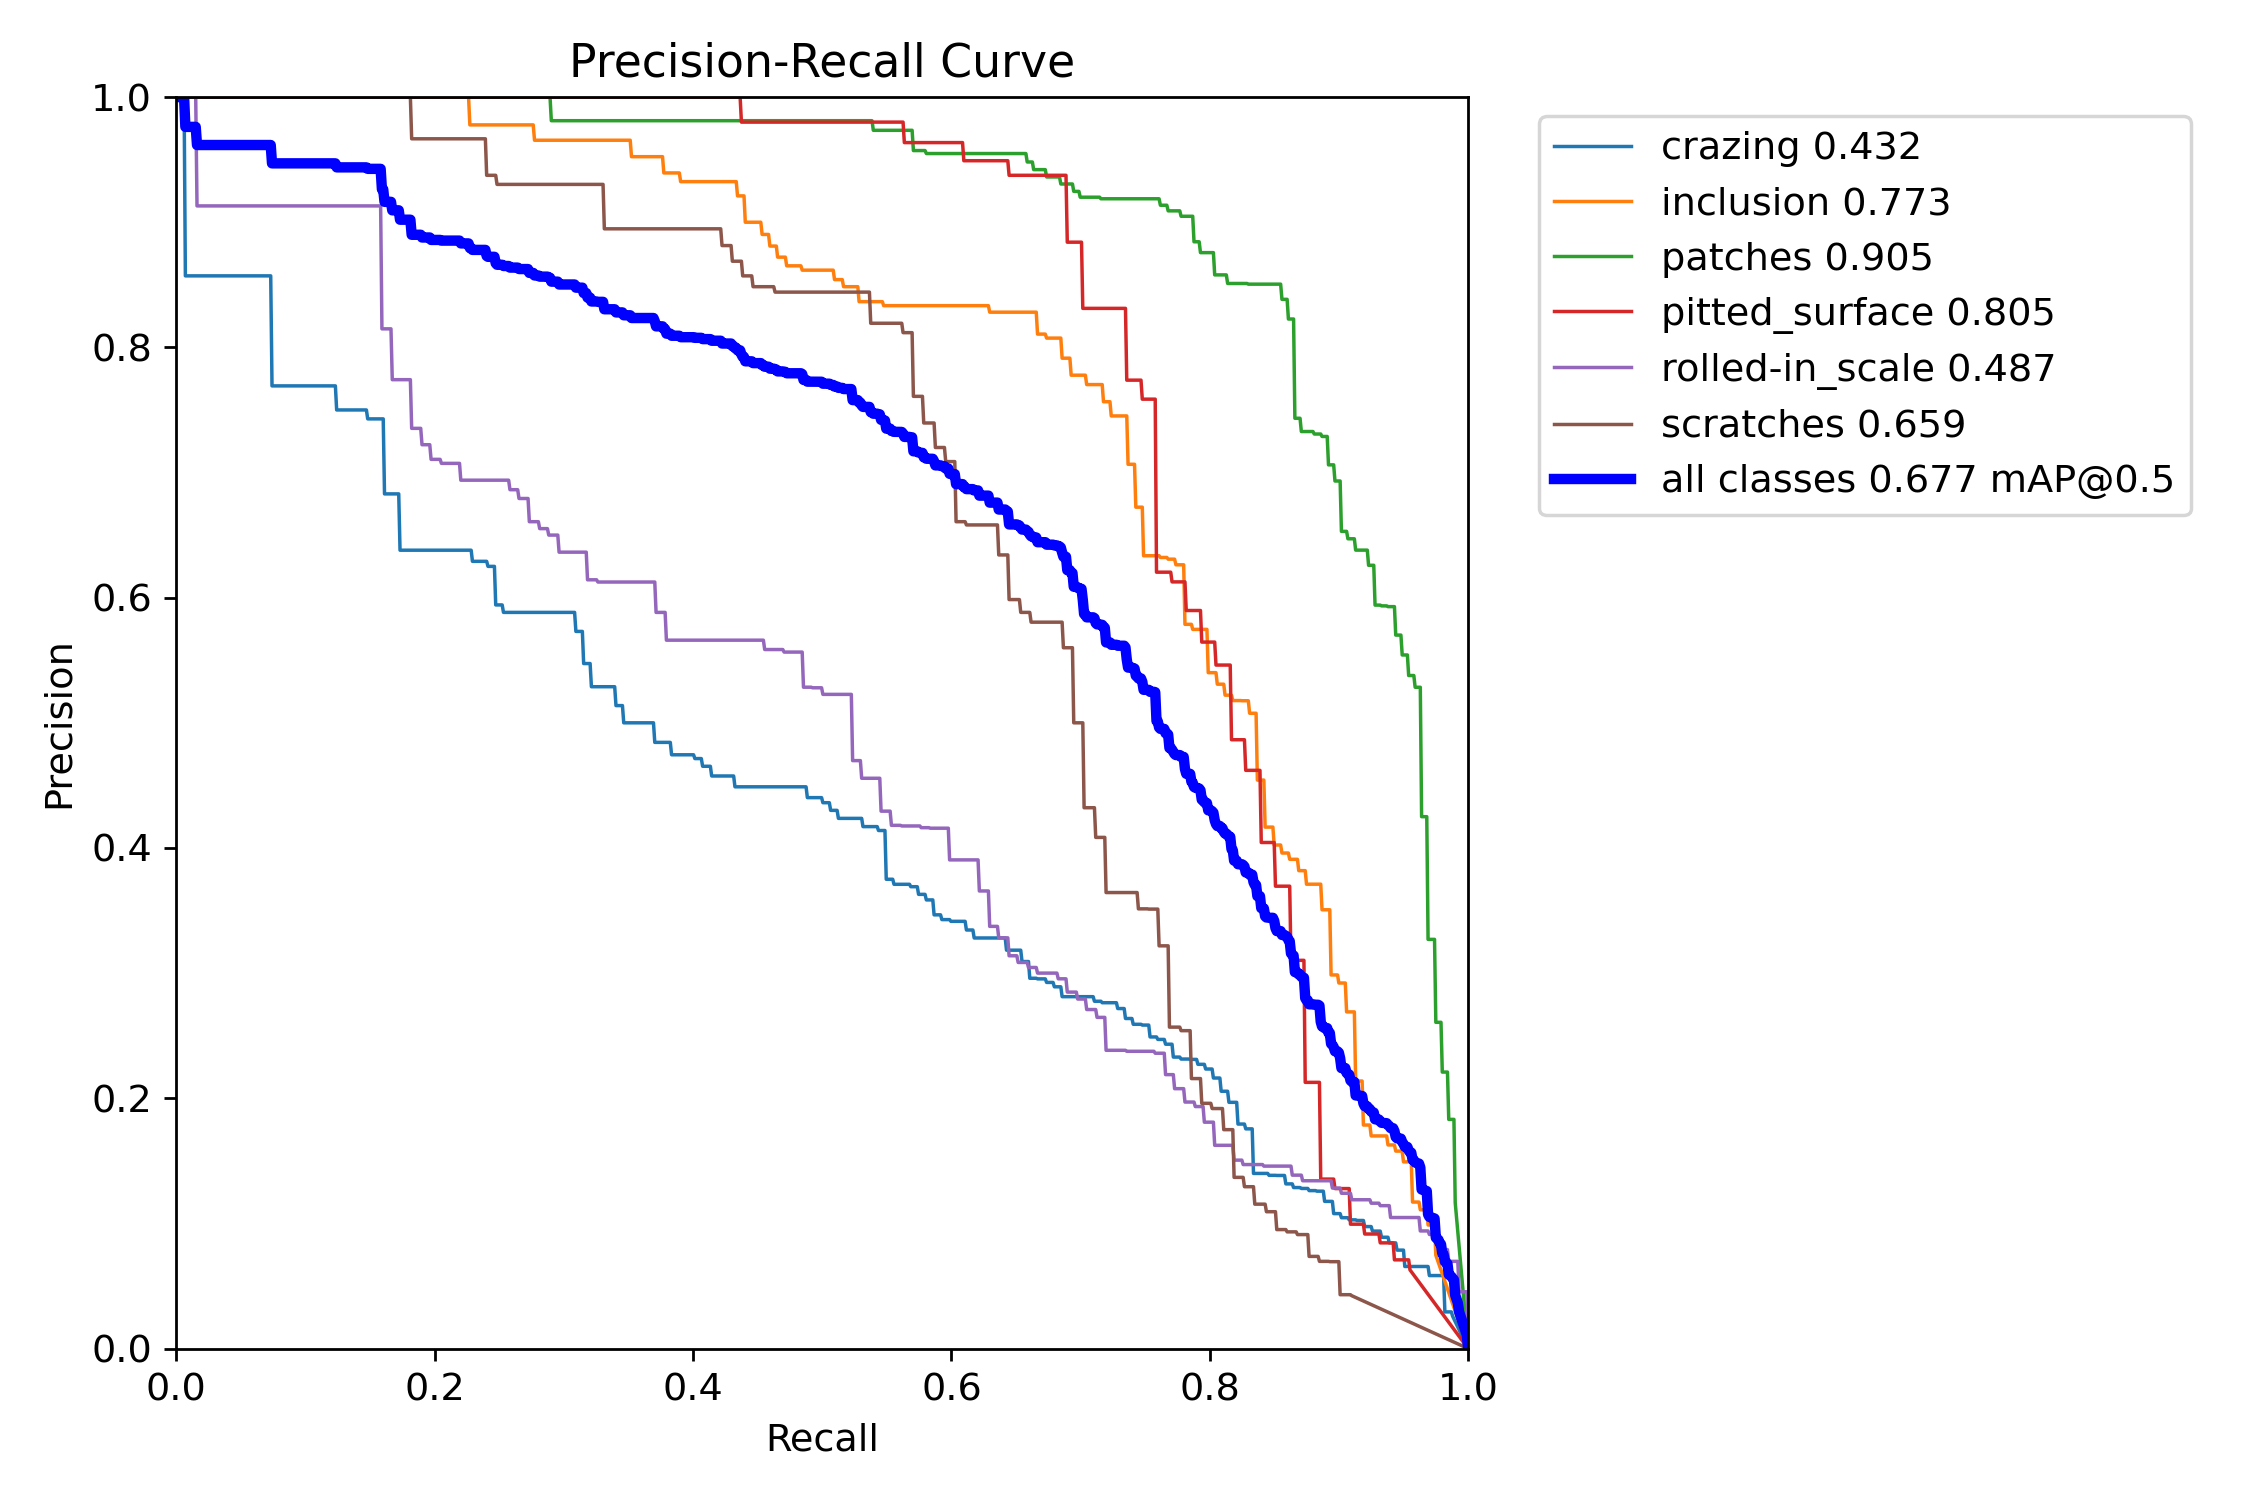
\includegraphics[width=0.45\linewidth]{img/BoxPR_curveI.png}
		\caption{نمودارهای \lr{precision}، \lr{Recall} و \lr{F1score} برحسب مقدار \lr{Confidence} و همچنین نمودار \lr{precision-Recall}}
	\end{figure}
	\newpage
	در بالا این معیارهارو توضیح دادیم. همانطور که مشخص است در اینجا در برخی از کلاس‌ها بهبود داشتیم و در برخی افت. مثلا در کلاس \lr{scratches} و \lr{rolled in scale} افت در عملکرد داشتیم اما در مابقی کلاس‌ها عملکردمون بهبود یافته است. این موضوع نشان می‌دهد که بلوک‌هایی که باعث افزایش توجه در برخی نواحی می‌شوند دقت را روی برخی کلاس‌ها می‌اندازند مثلا خراش‌ها که در طول قطعه پیوسته وجود دارند، توسط این بلوک‌ها قابل تشخیص نمی‌شوند و یا دقت پایینتر می‌آید اما به طور کلی این روش تا حدودی باعث بهبود دقت مدل شده است.
	
	در طبقه‌بندی کلاس‌ها نیز ماتریس درهمریختگی به صورت شکل زیر می‌شود. همانطور که مشخص است تا حد زیادی بهبود در نتایج این ماتریس دیده می‌شود. یعنی تا حد خوبی توانستیم تشخیص اشتباه پس‌زمینه با کلاس‌های دیگر را توسط مدل کاهش دهیم.
	
	\begin{figure}[H]
		\centering
		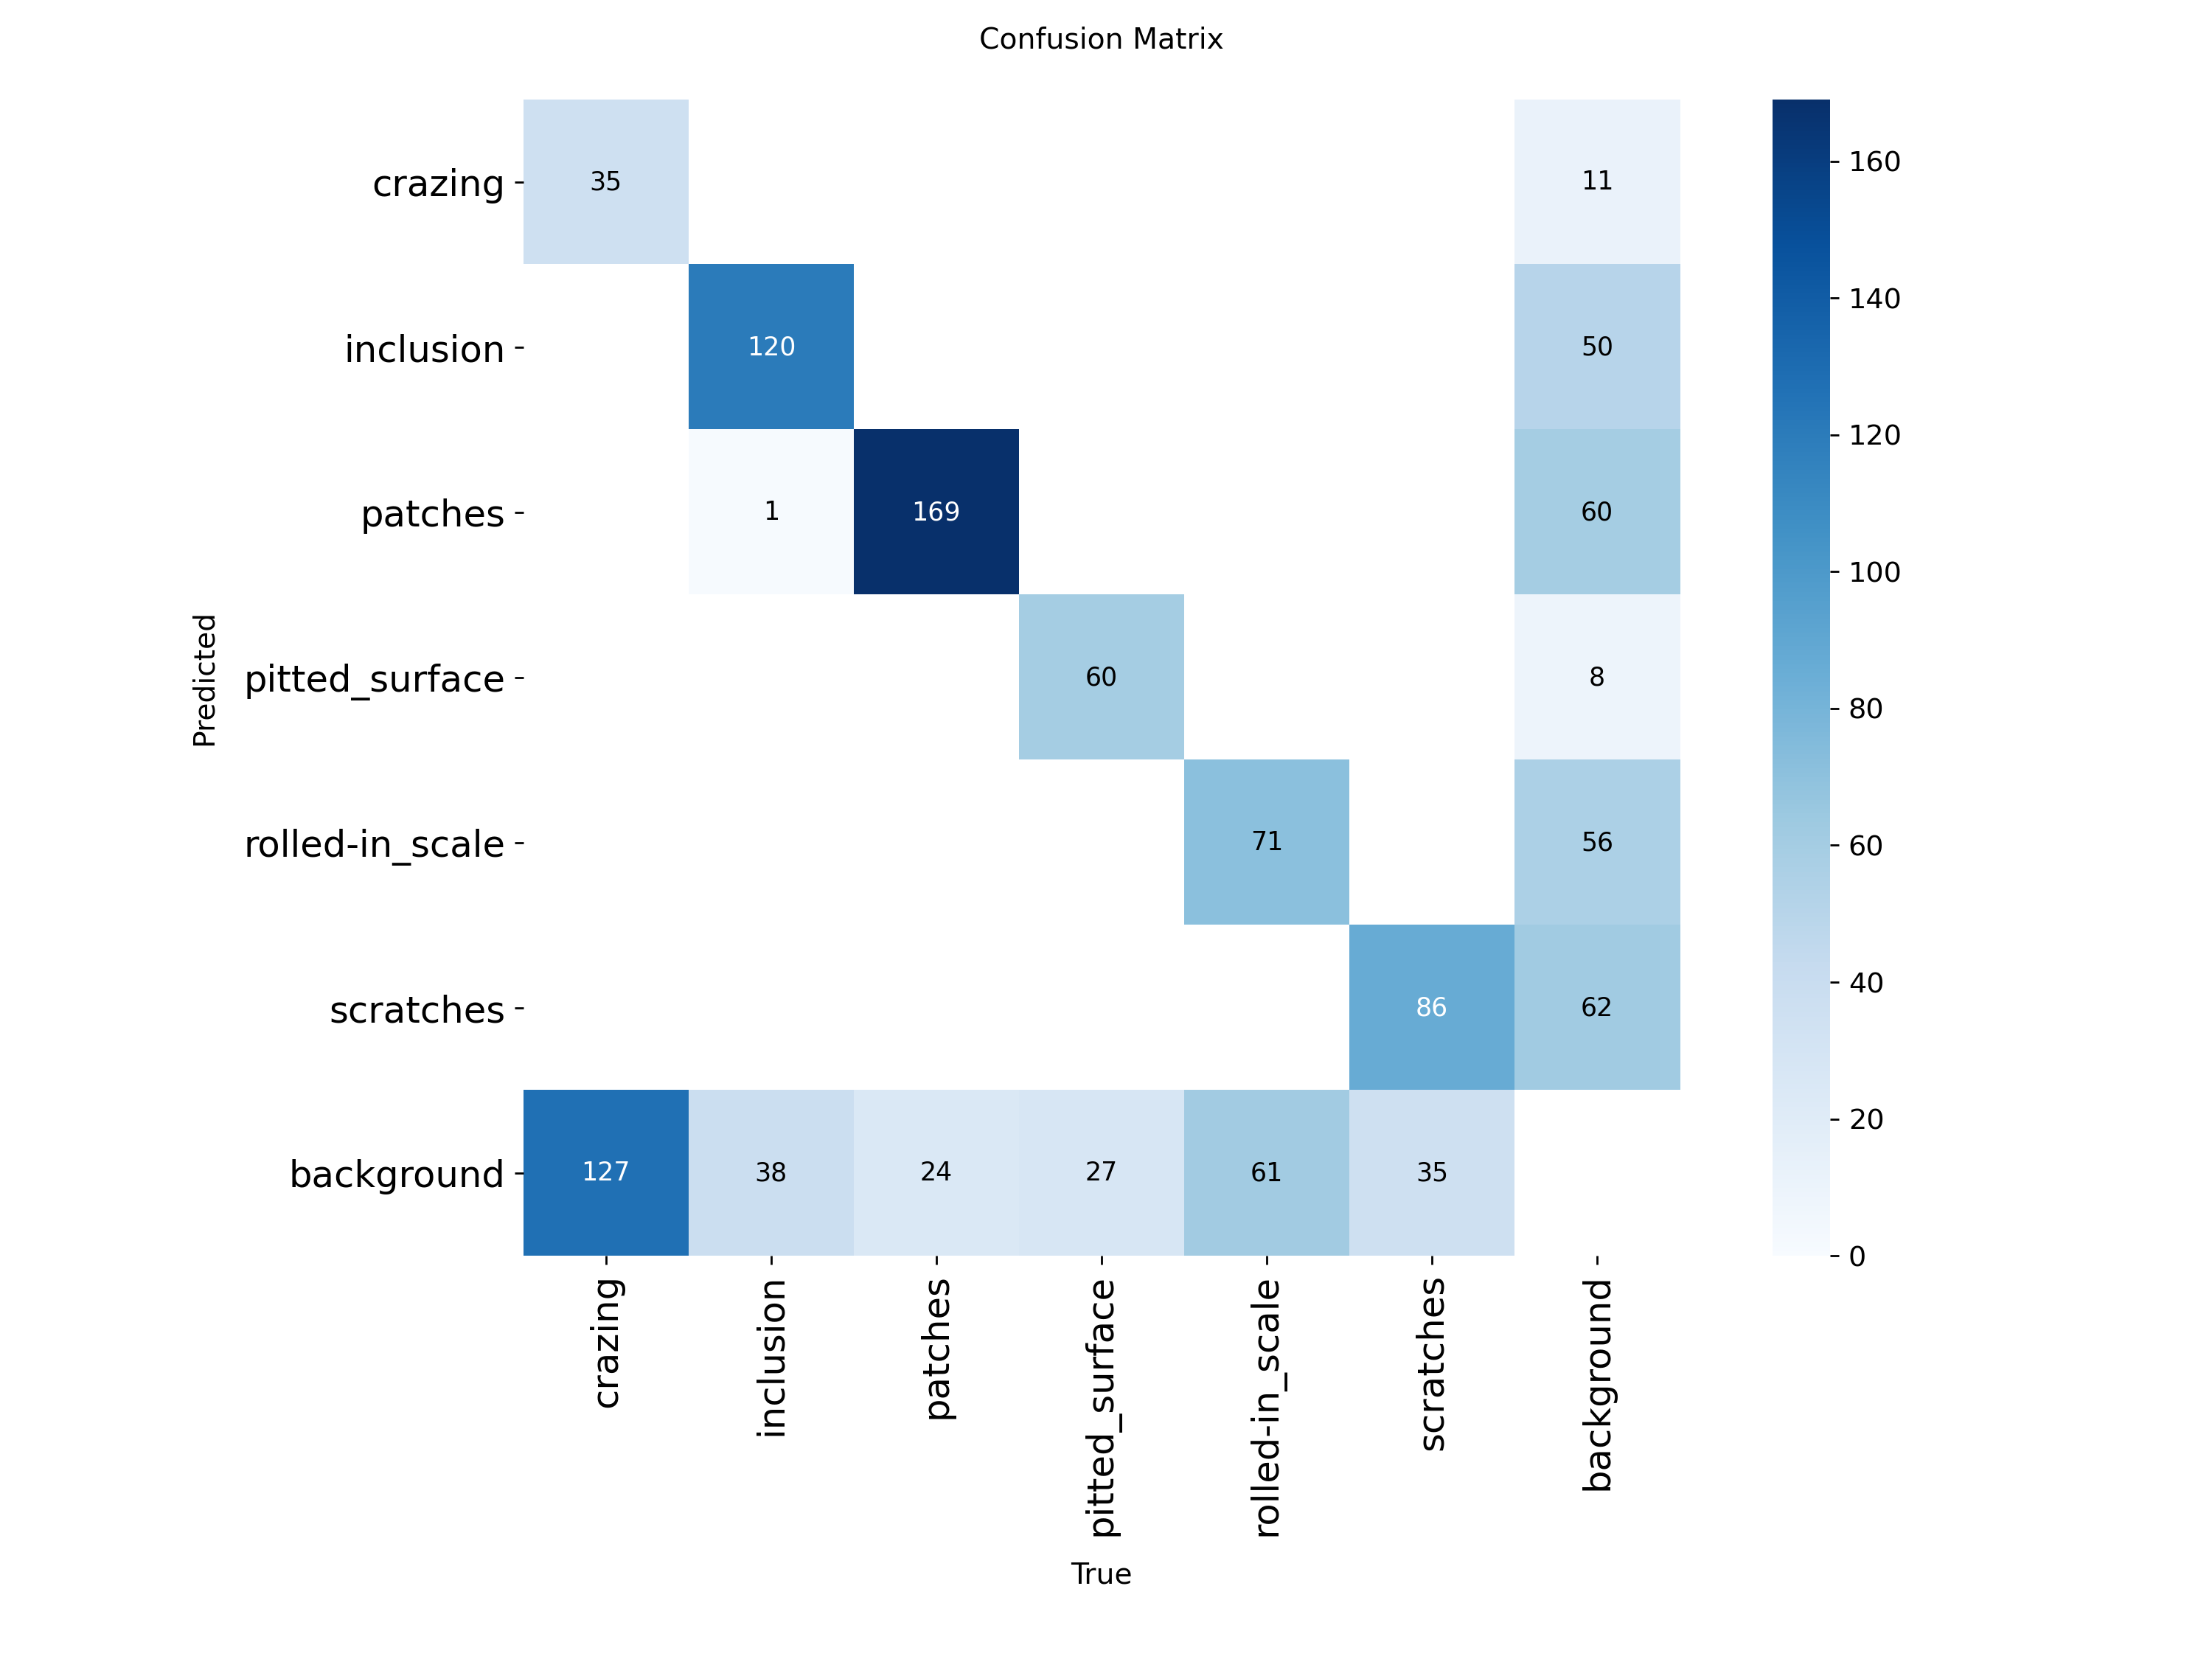
\includegraphics[width=0.3\linewidth]{img/confusion_matrixI.png}
		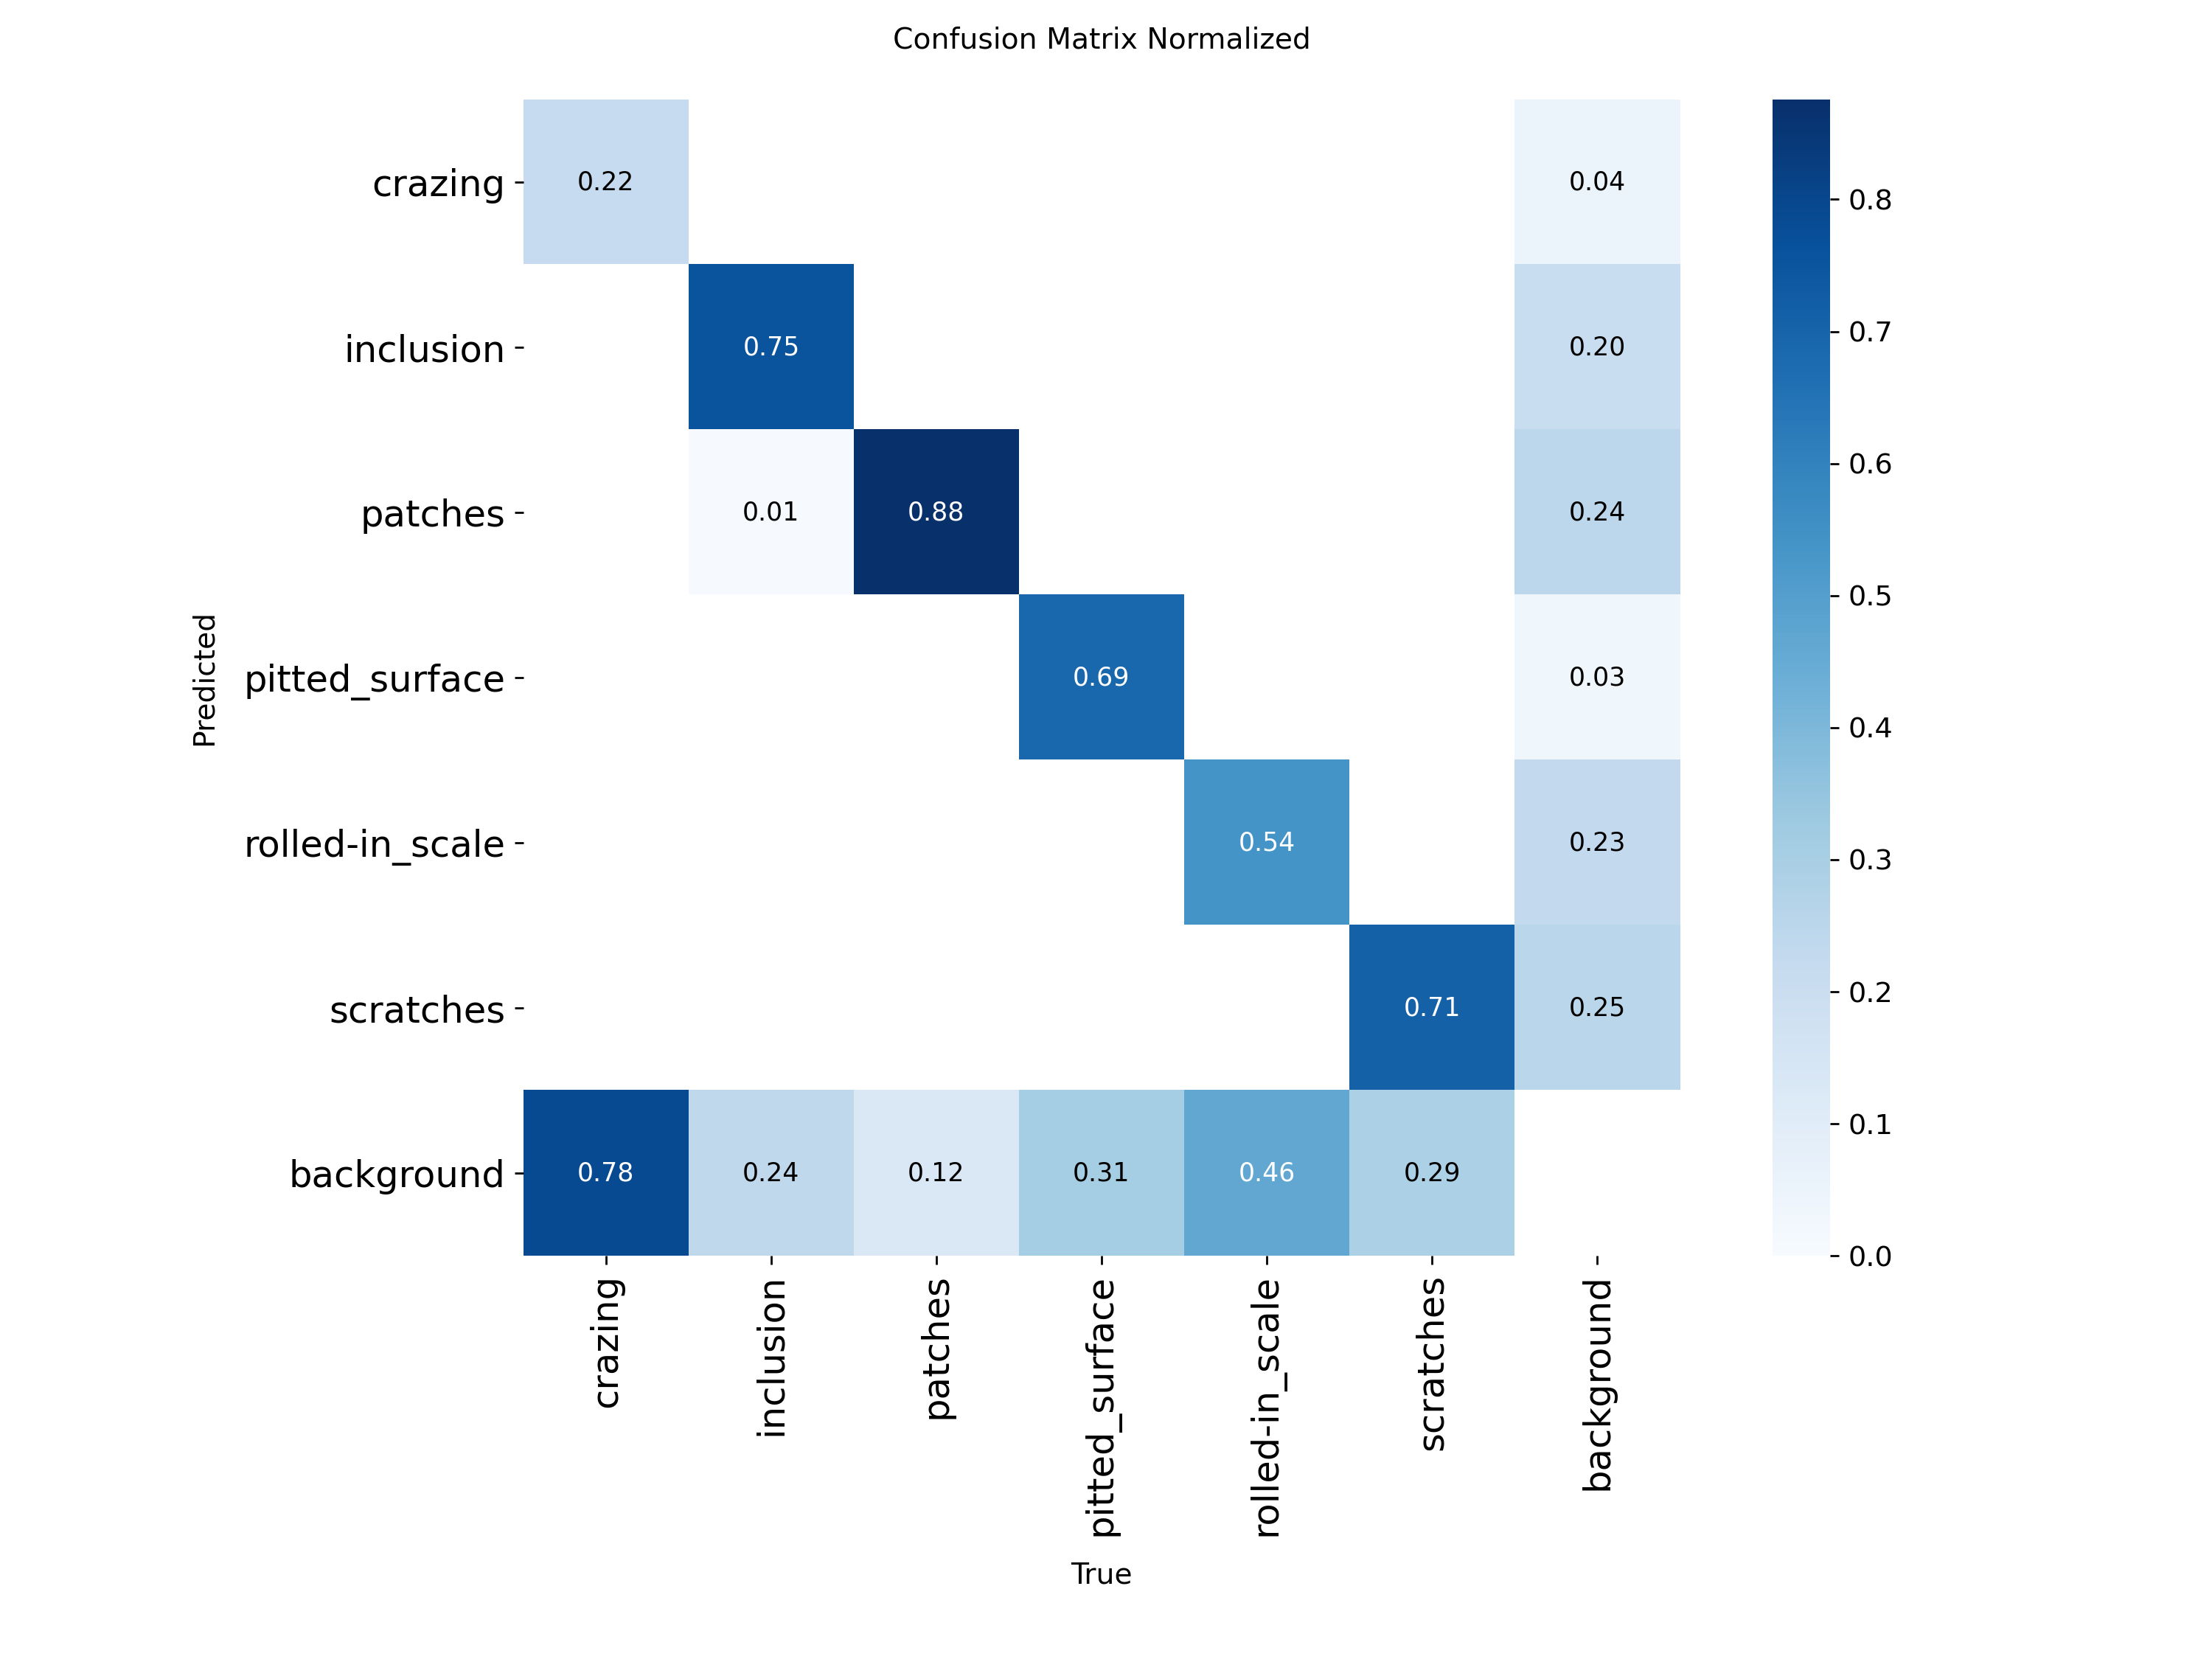
\includegraphics[width=0.3\linewidth]{img/confusion_matrix_normalizedI.png}
		\caption{ماتریس درهمریختگی}
	\end{figure}
	نمونه‌ای از تشخیص مدل به صورت زیر می‌باشد:
	\begin{figure}[H]
		\centering
		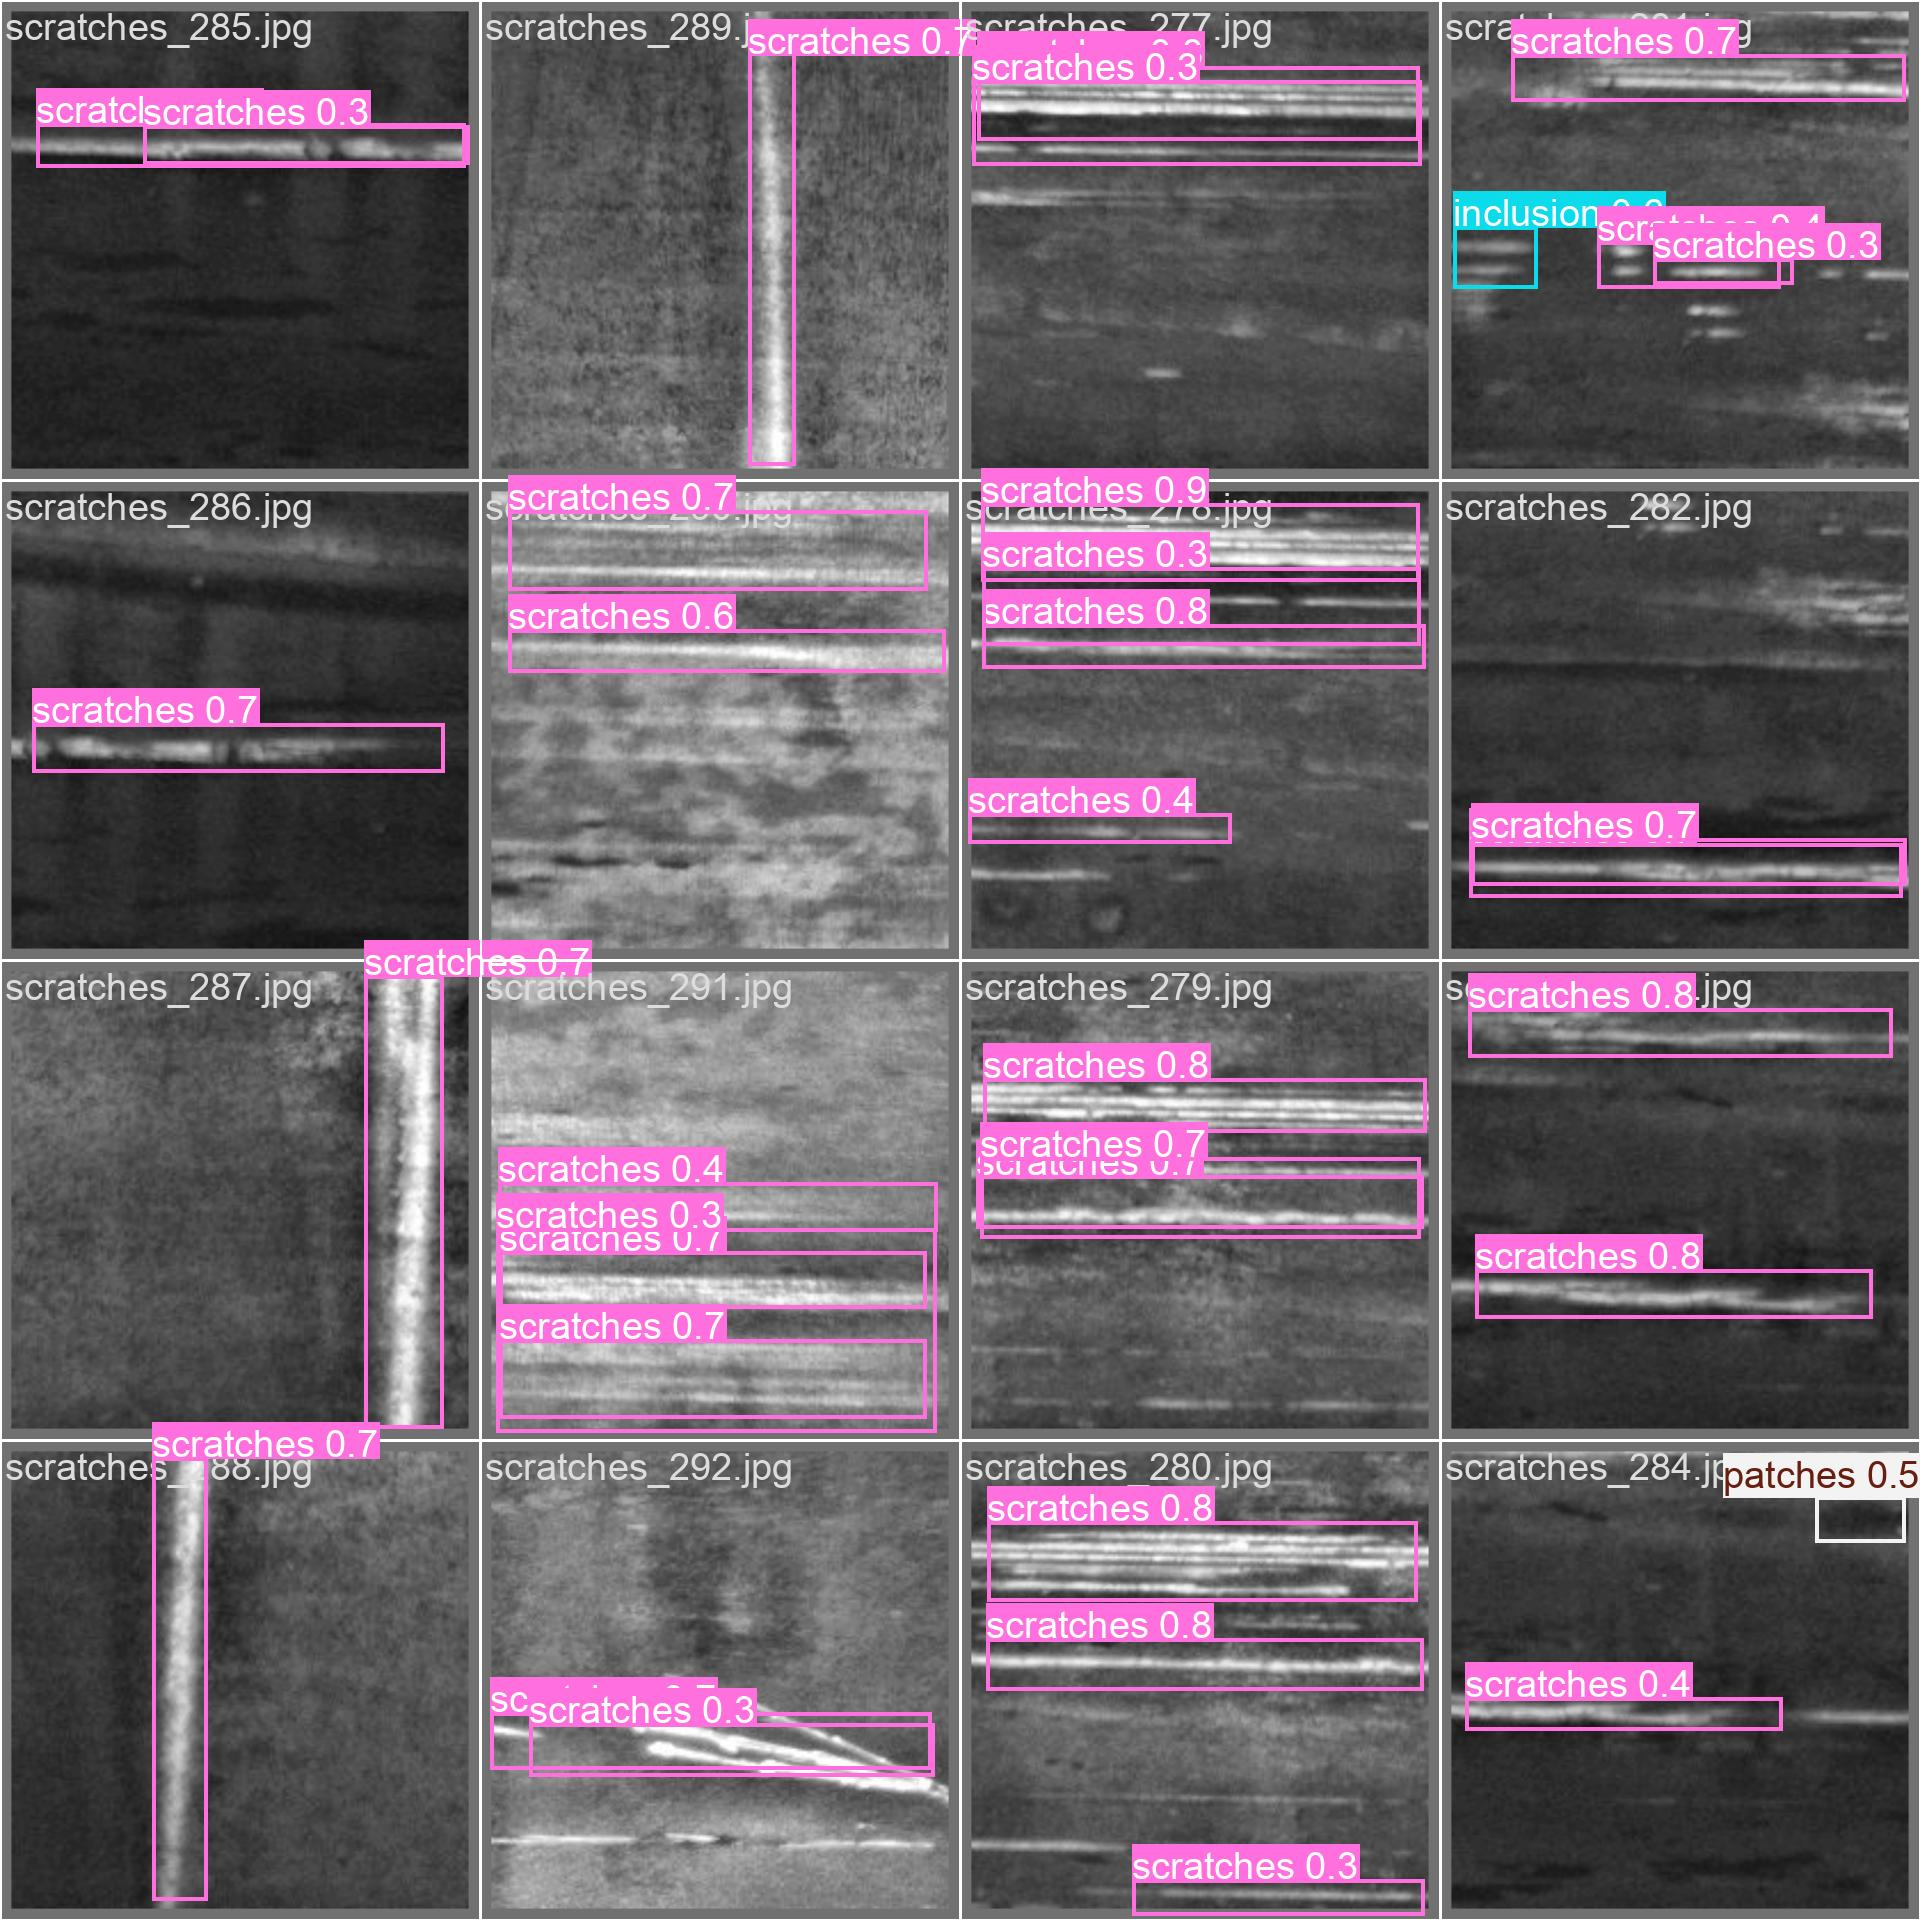
\includegraphics[width=0.2\linewidth]{img/val_batch0_predi.jpg}
		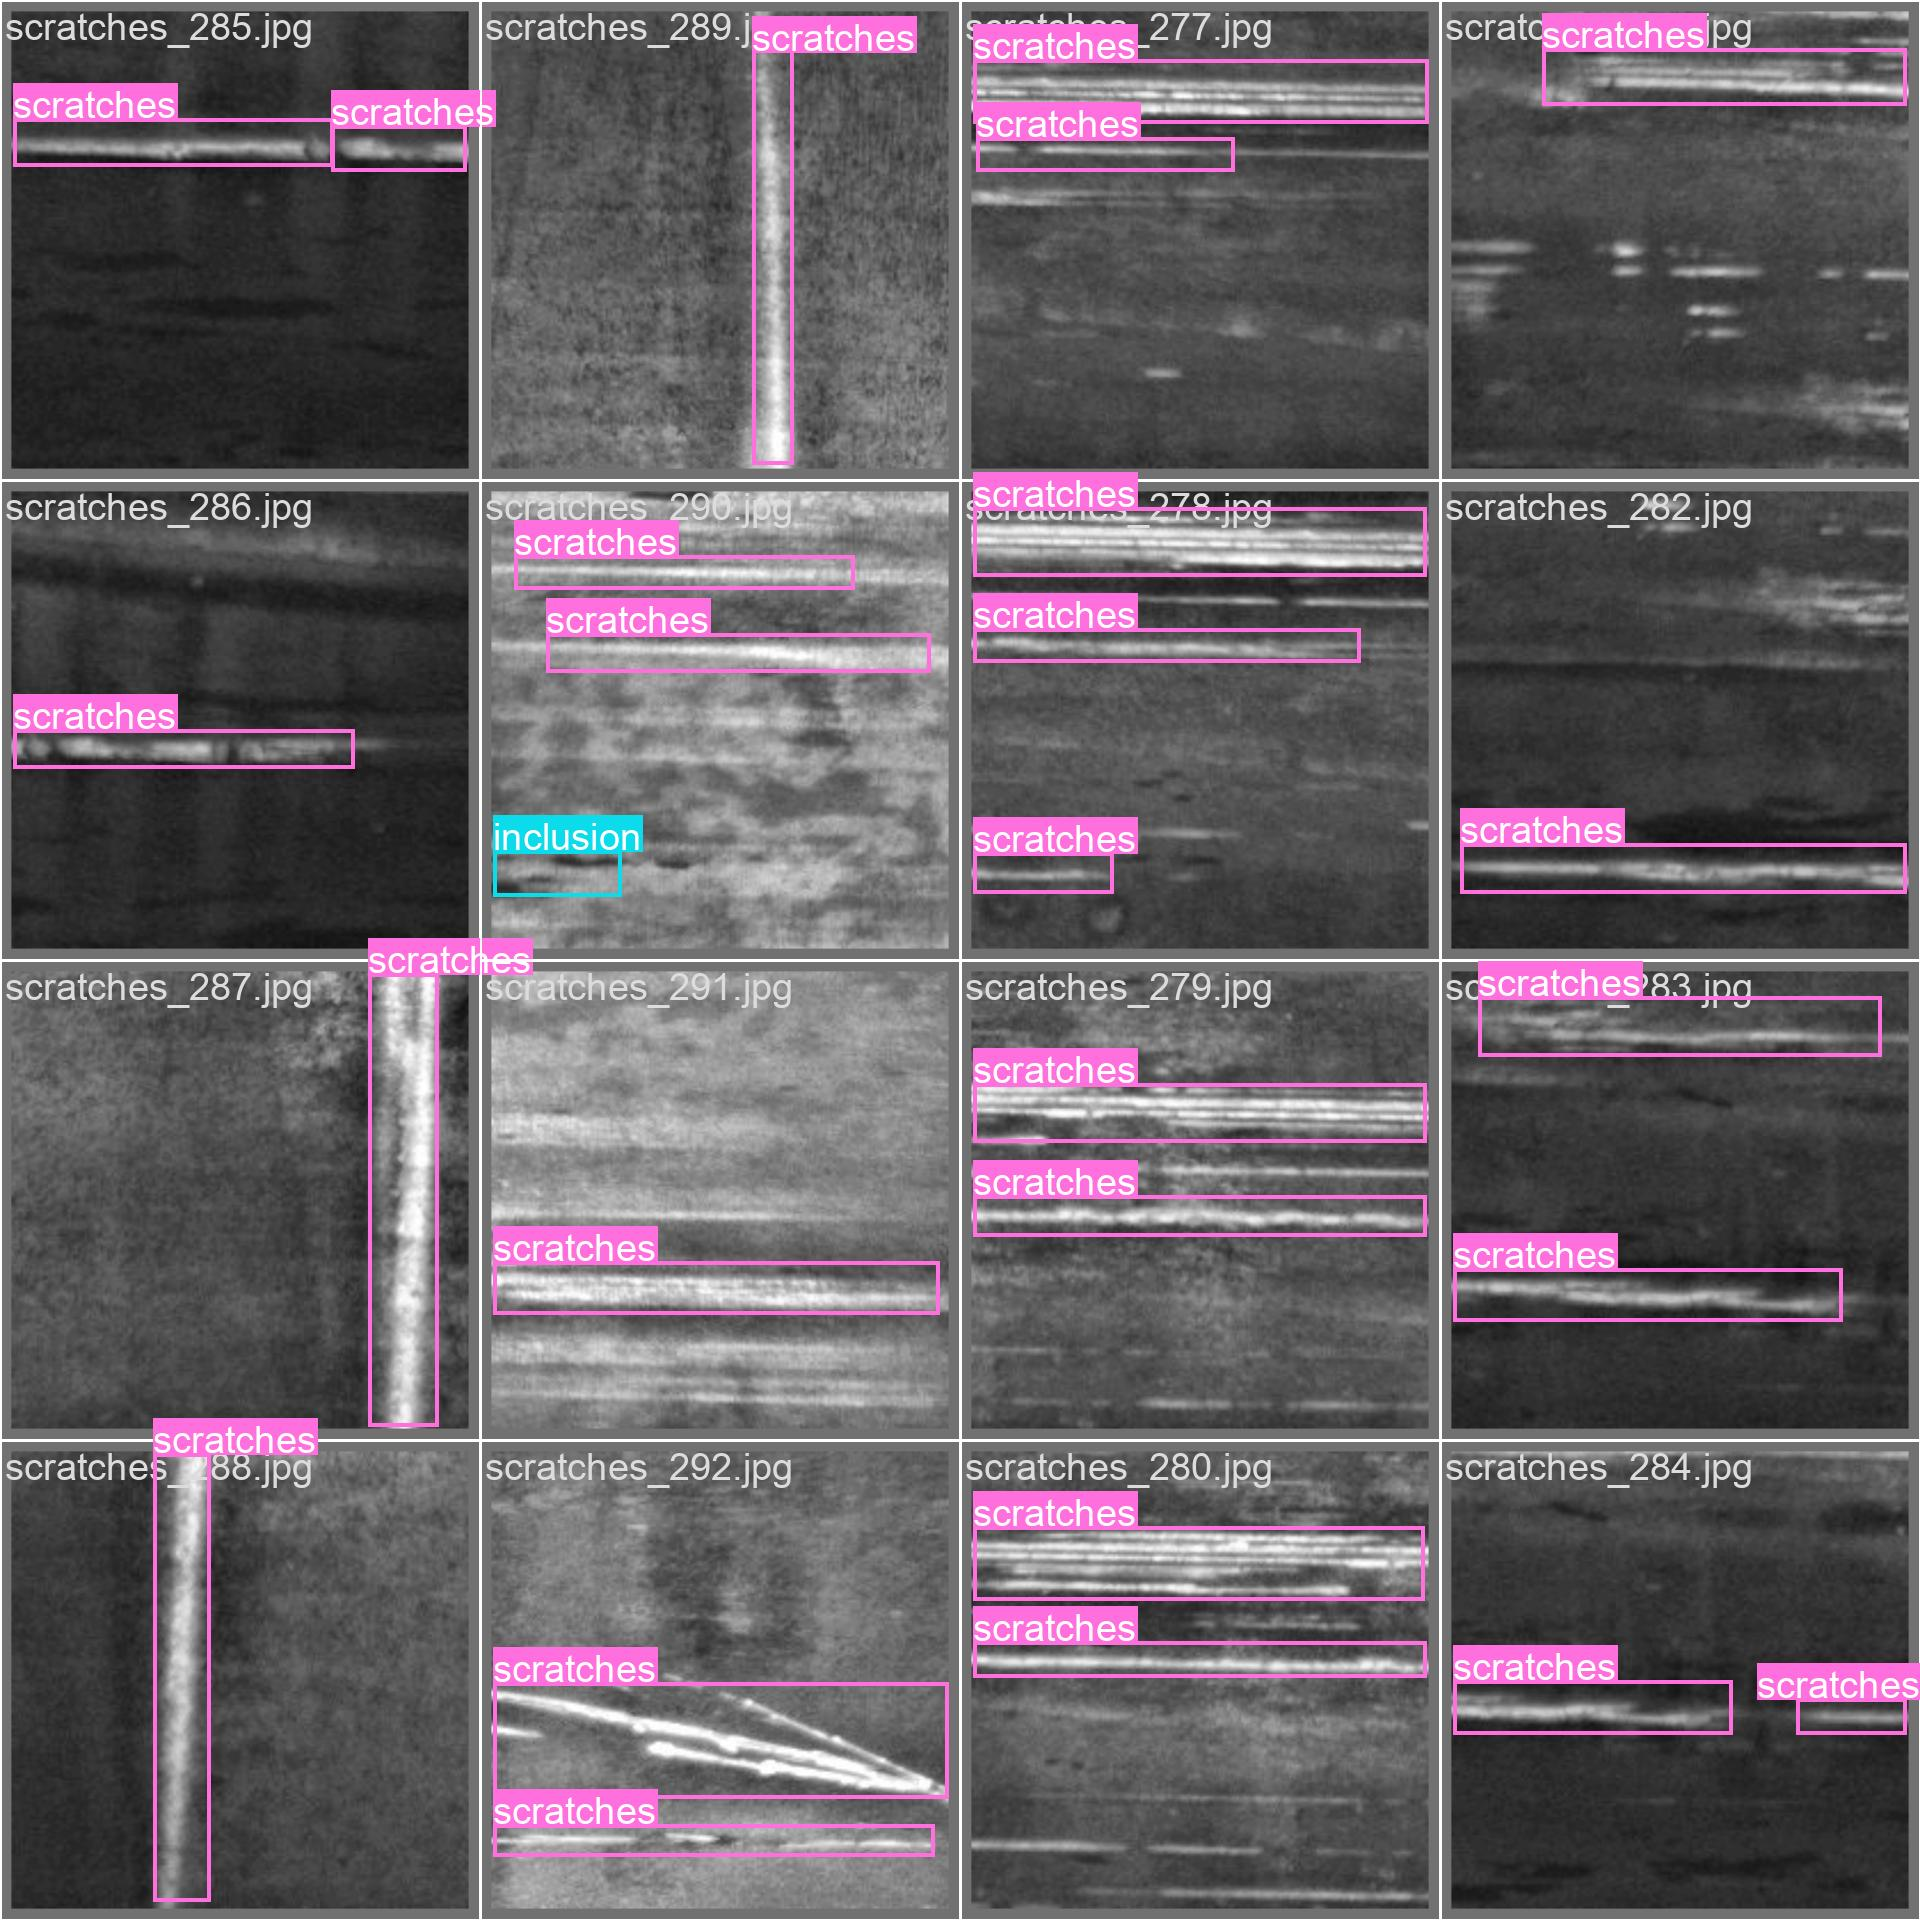
\includegraphics[width=0.2\linewidth]{img/val_batch0_labelsi.jpg}
		
		\vspace{0.3cm}
		
		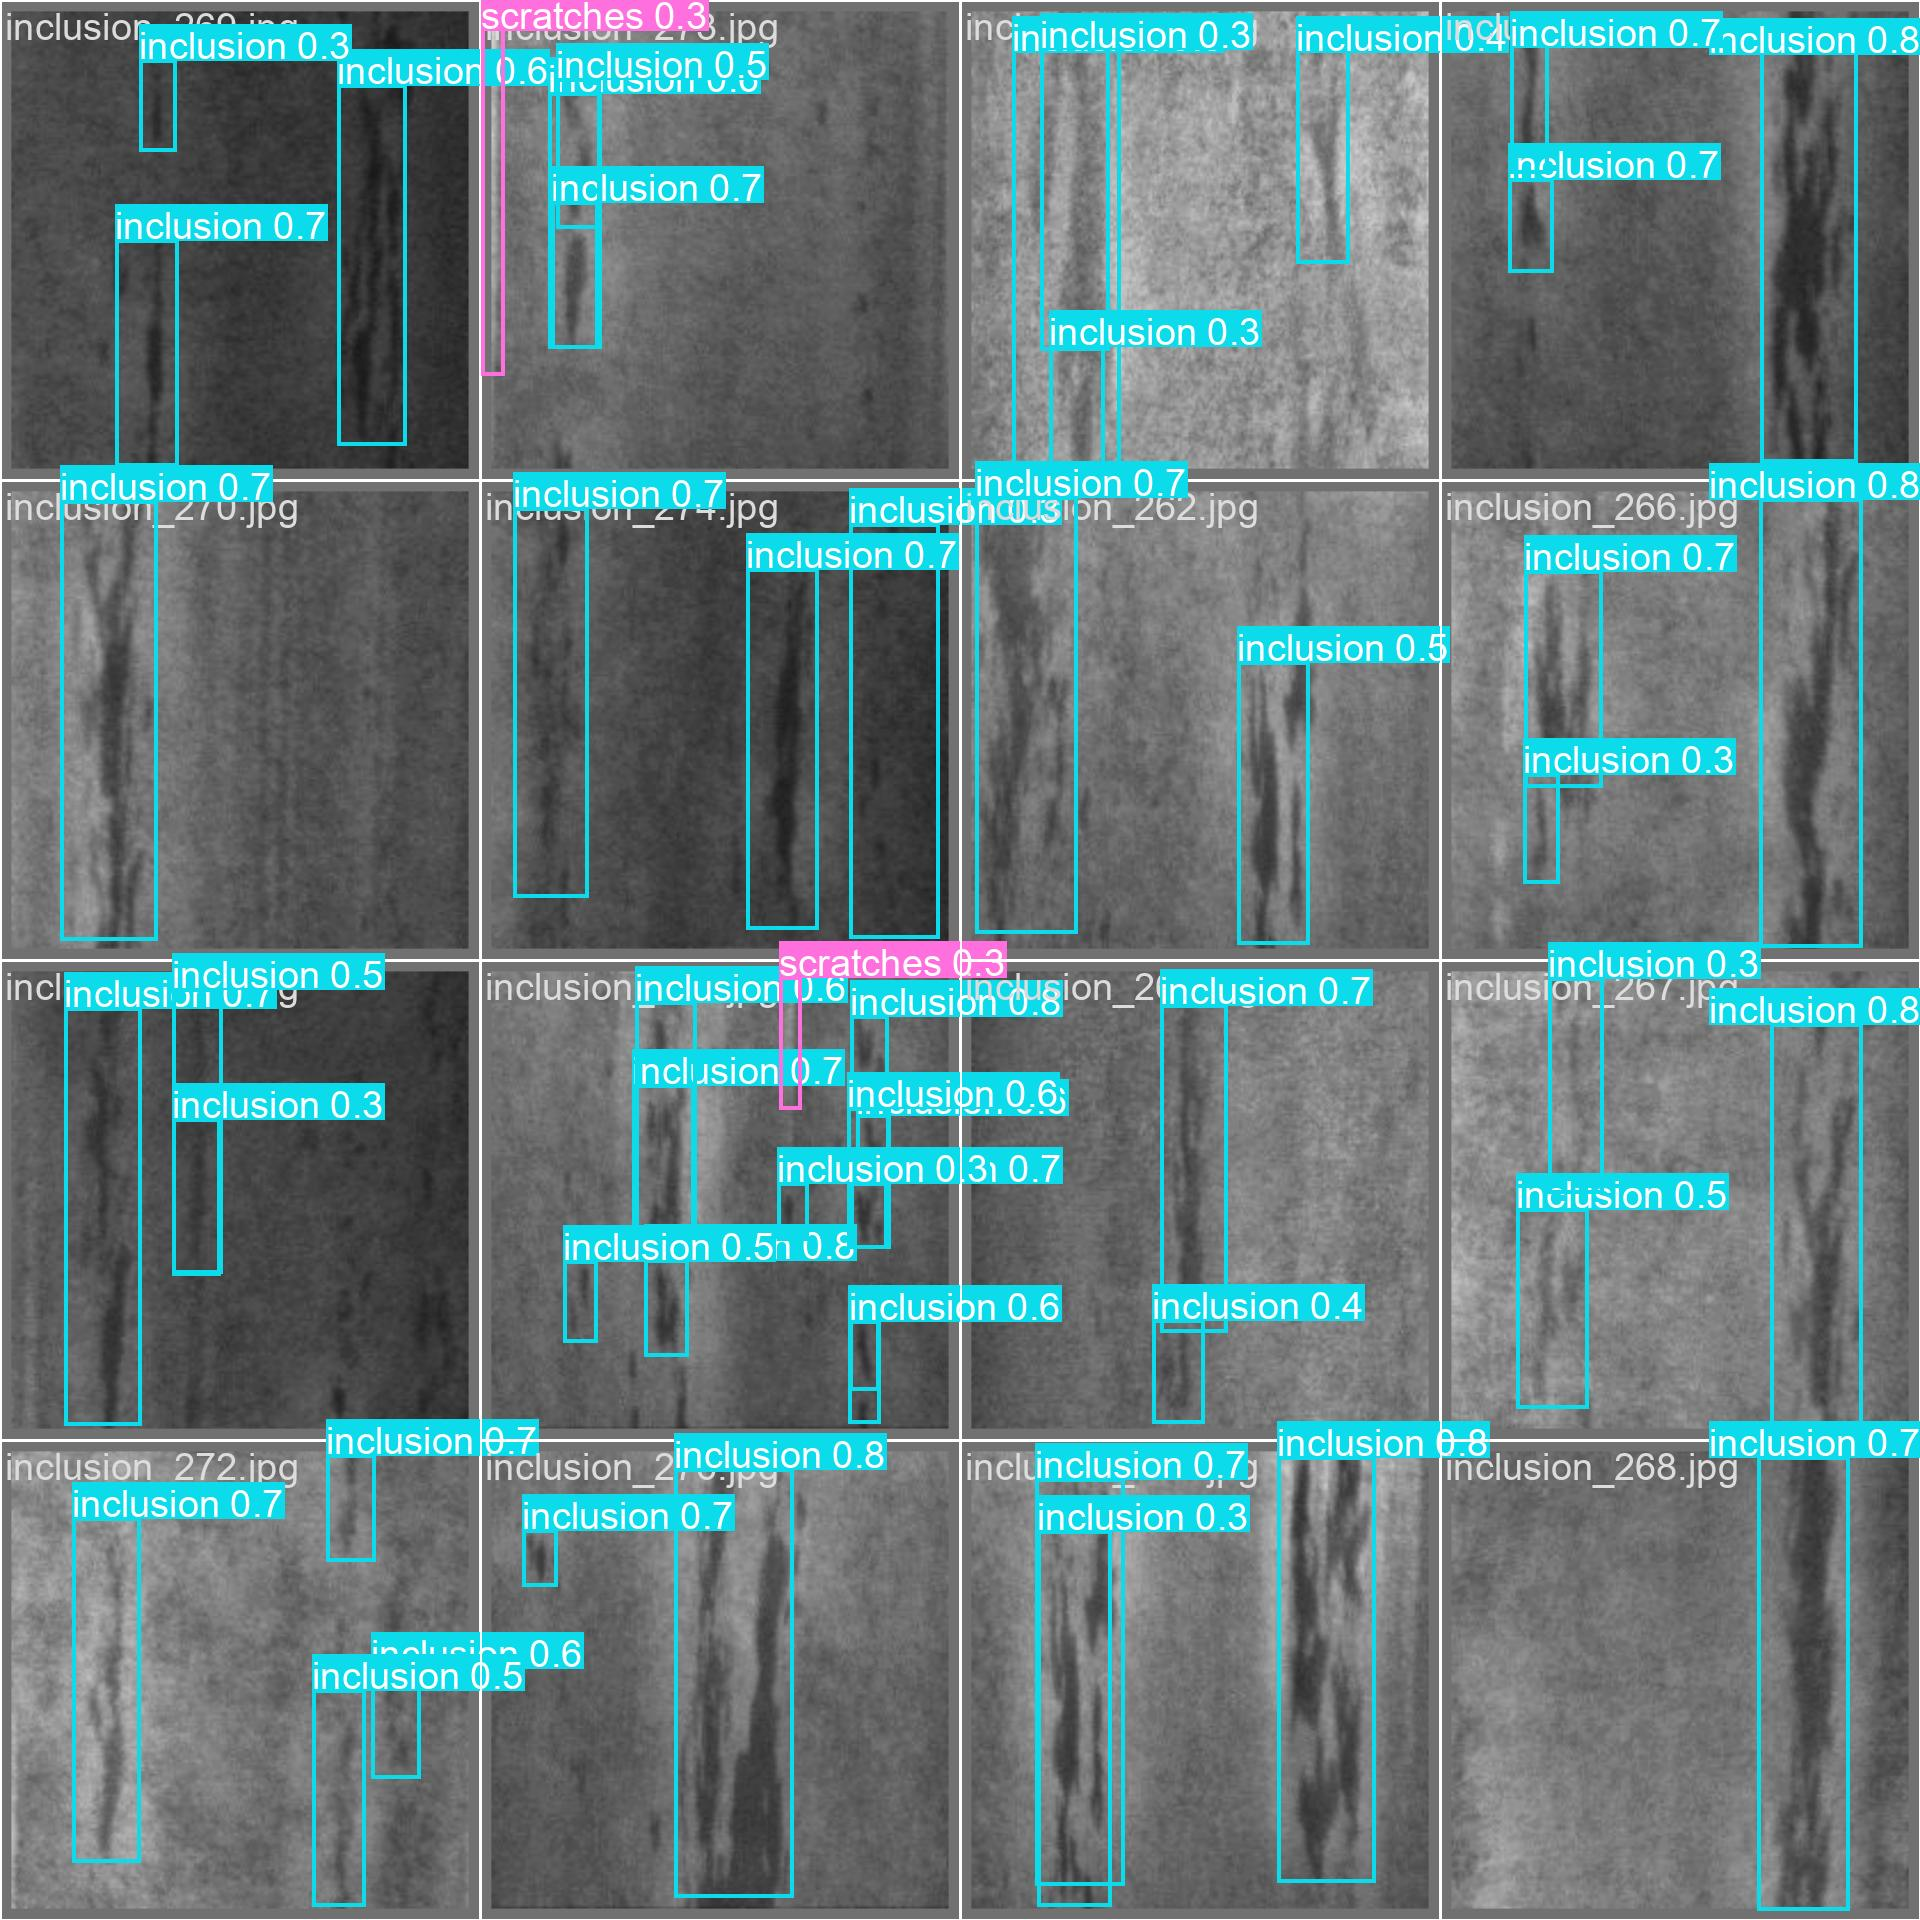
\includegraphics[width=0.2\linewidth]{img/val_batch2_predi.jpg}
		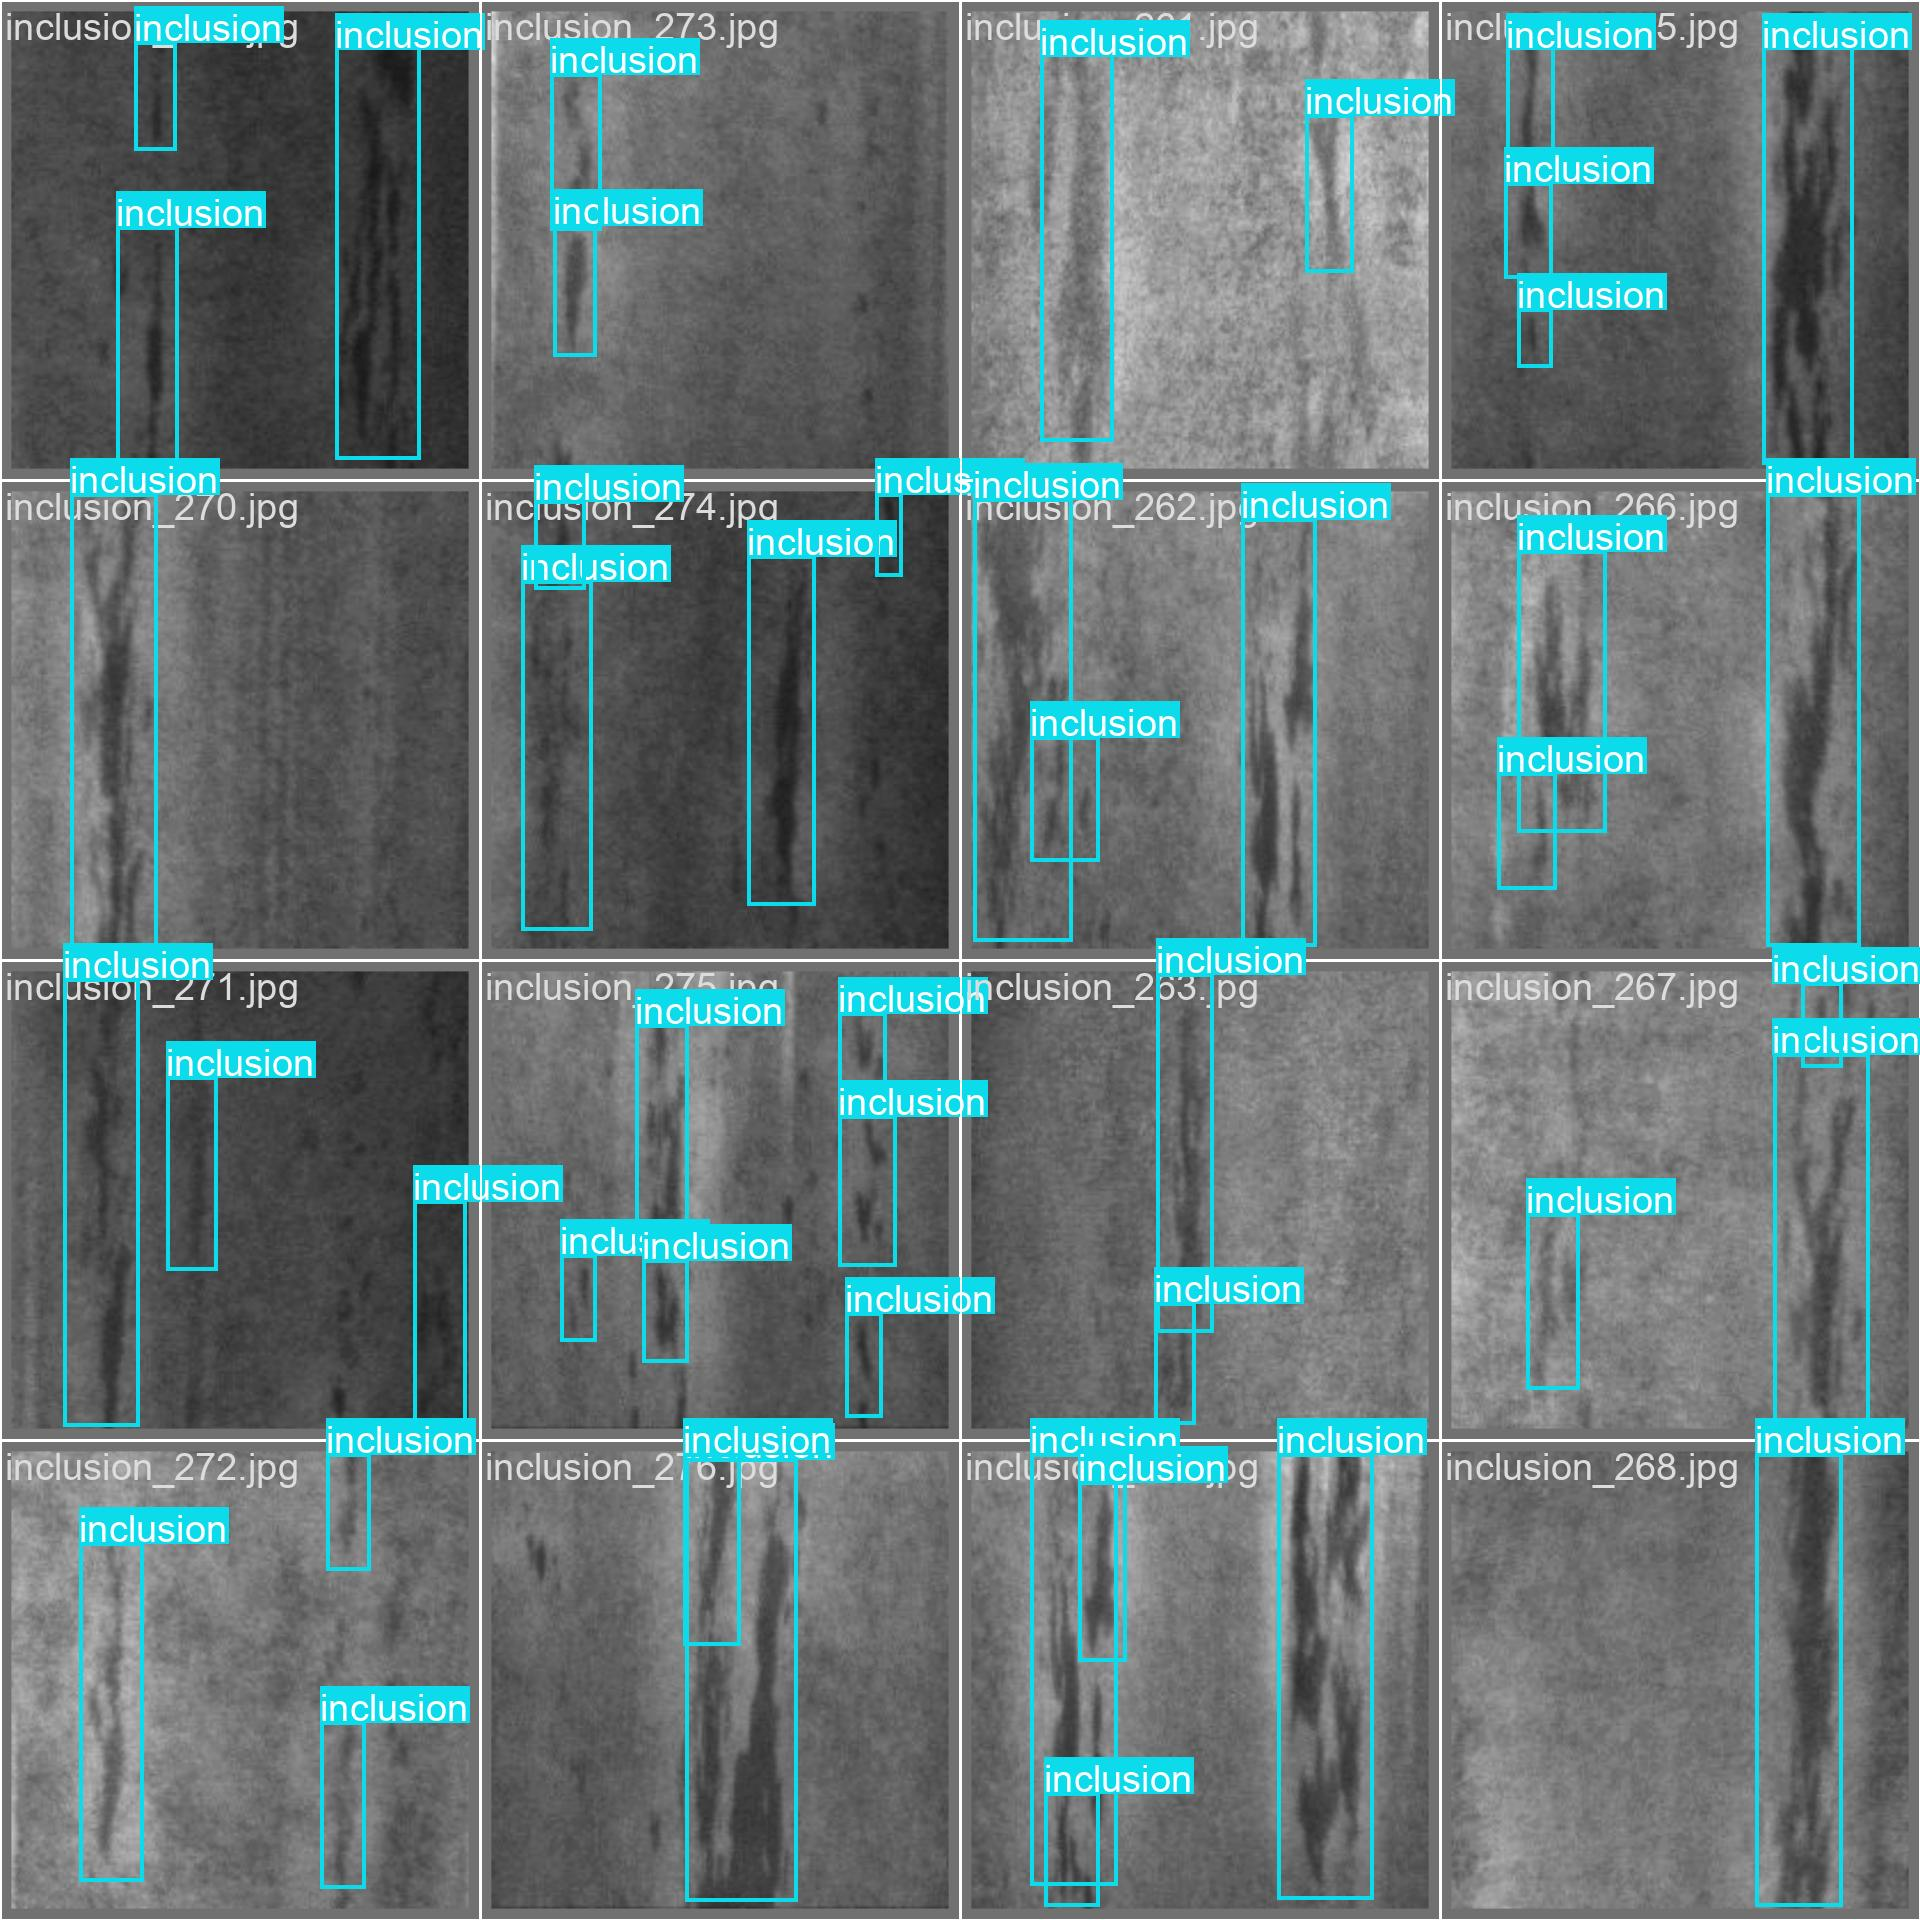
\includegraphics[width=0.2\linewidth]{img/val_batch2_labelsi.jpg}
		\caption{نمونه‌هایی از تشخیص مدل}
	\end{figure}
	
	
	
	\subsection{پیاده‌سازی مدل \lr{YOLOv11m}}
	\begin{figure}[H]
		\centering
		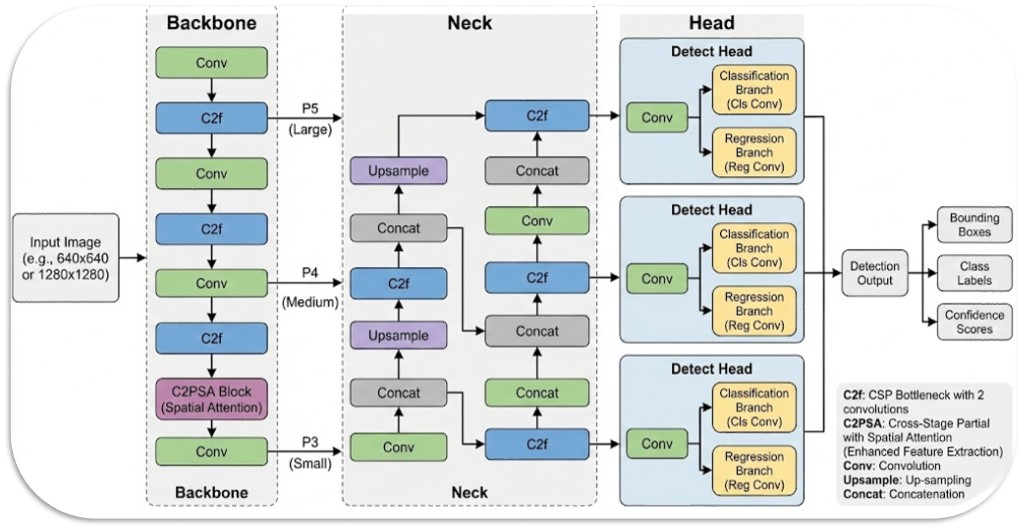
\includegraphics[width=0.8\linewidth]{img/yolov11m.jpg}
		\caption{ساختار مدل \lr{yolov11m} (تصویر ساخته شده با هوش مصنوعی)}
	\end{figure}
	
	
	در این بخش، مدل \lr{YOLO11m} به عنوان یک مدل میان‌رده (\lr{Medium}) از خانواده \lr{YOLO11} مورد استفاده قرار گرفت. این مدل نسبت به نسخه‌های \lr{Nano} و \lr{Small} دارای عمق و عرض شبکه بیشتر بوده و ظرفیت یادگیری بالاتری دارد. 
	
	\lr{YOLO11m} با بهره‌گیری از معماری بهینه‌شده، ساختار چندمقیاسی در بخش \lr{Neck} و سر آشکارساز تفکیک‌شده (\lr{Decoupled Head})، قادر به استخراج ویژگی‌های پیچیده‌تر و مدل‌سازی دقیق‌تر اهداف در مقیاس‌های مختلف است. افزایش تعداد پارامترها در این مدل موجب بهبود دقت تشخیص می‌شود، هرچند هزینه محاسباتی و مصرف حافظه نیز افزایش می‌یابد.
	
	\subsection{تنظیمات آموزش}
	
	مدل با تنظیمات زیر آموزش داده شد:
	
	\begin{itemize}
		\item اندازه ورودی تصاویر: $640 \times 640$
		\item تعداد دوره آموزش: 200
		\item اندازه دسته (\lr{Batch Size}): 16
		\item بهینه‌ساز: \lr{AdamW}
		\item نرخ یادگیری اولیه: $10^{-3}$
		\item زمان گرم‌سازی: 5 دوره
		\item غیرفعال‌سازی \lr{Mosaic}، \lr{MixUp} و \lr{CutMix}
		\item استفاده از افزایش داده رنگی (\lr{HSV augmentation})
	\end{itemize}
	
	استفاده از \lr{AdamW} موجب بهبود تنظیم وزن‌ها و کاهش بیش‌برازش شده و غیرفعال‌سازی \lr{Mosaic} باعث حفظ ساختار طبیعی نمونه‌ها گردید.
	
	
	نتایج مربوط به آموزش مدل به صورت زیر است:
	\begin{figure}[H]
		\centering
		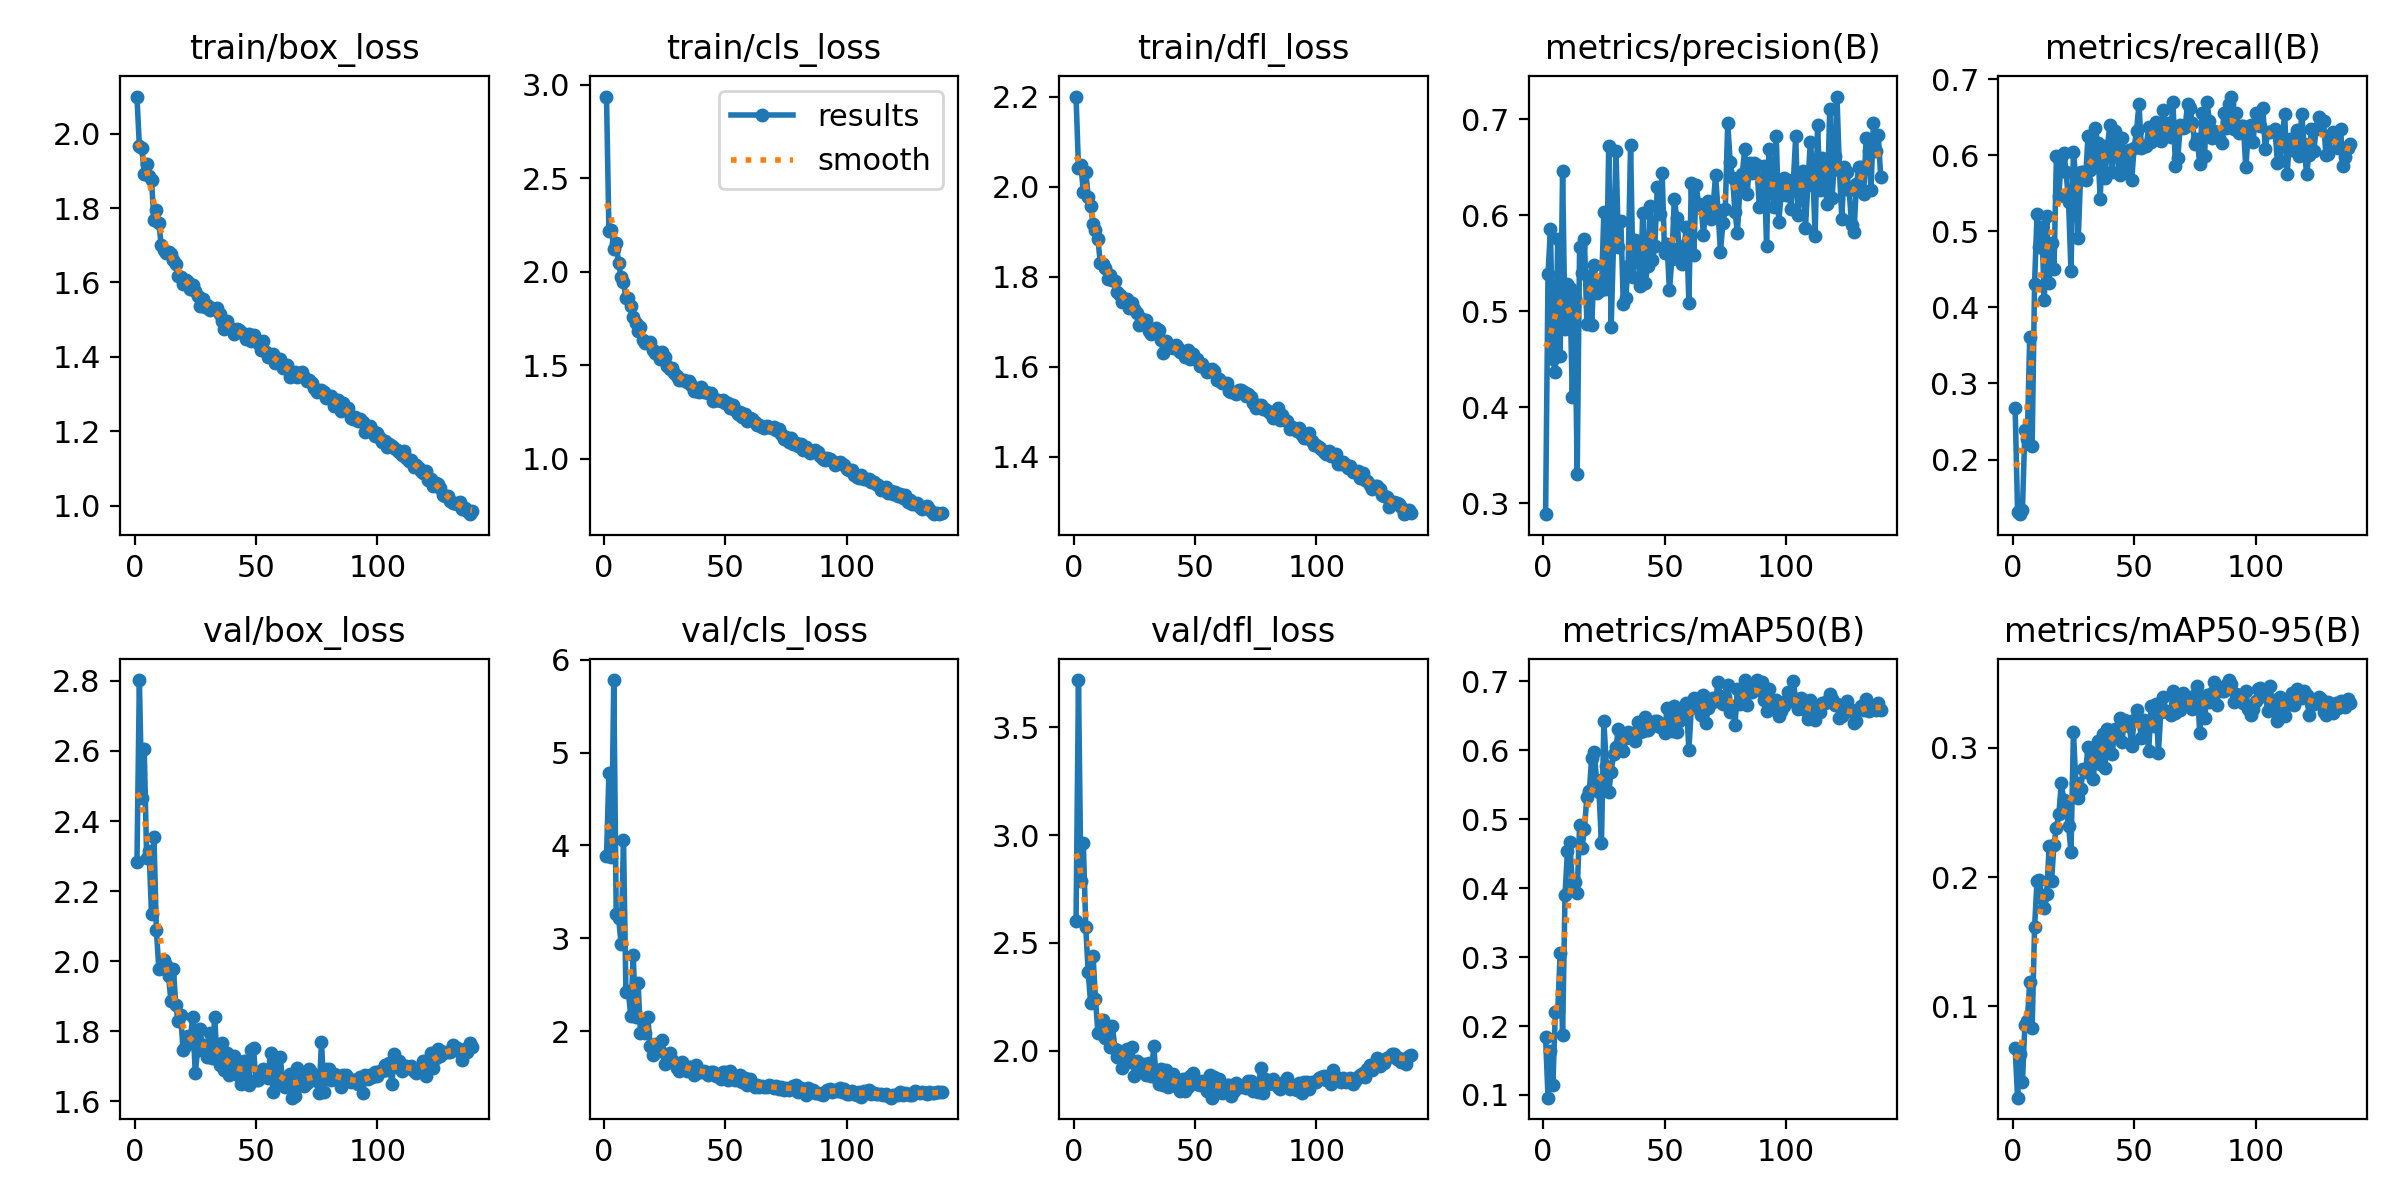
\includegraphics[width=0.9\linewidth]{img/resultsm.png}
		\caption{نمودارهای مربوط به روند آموزش مدل}
	\end{figure}
	\begin{figure}[H]
		\centering
		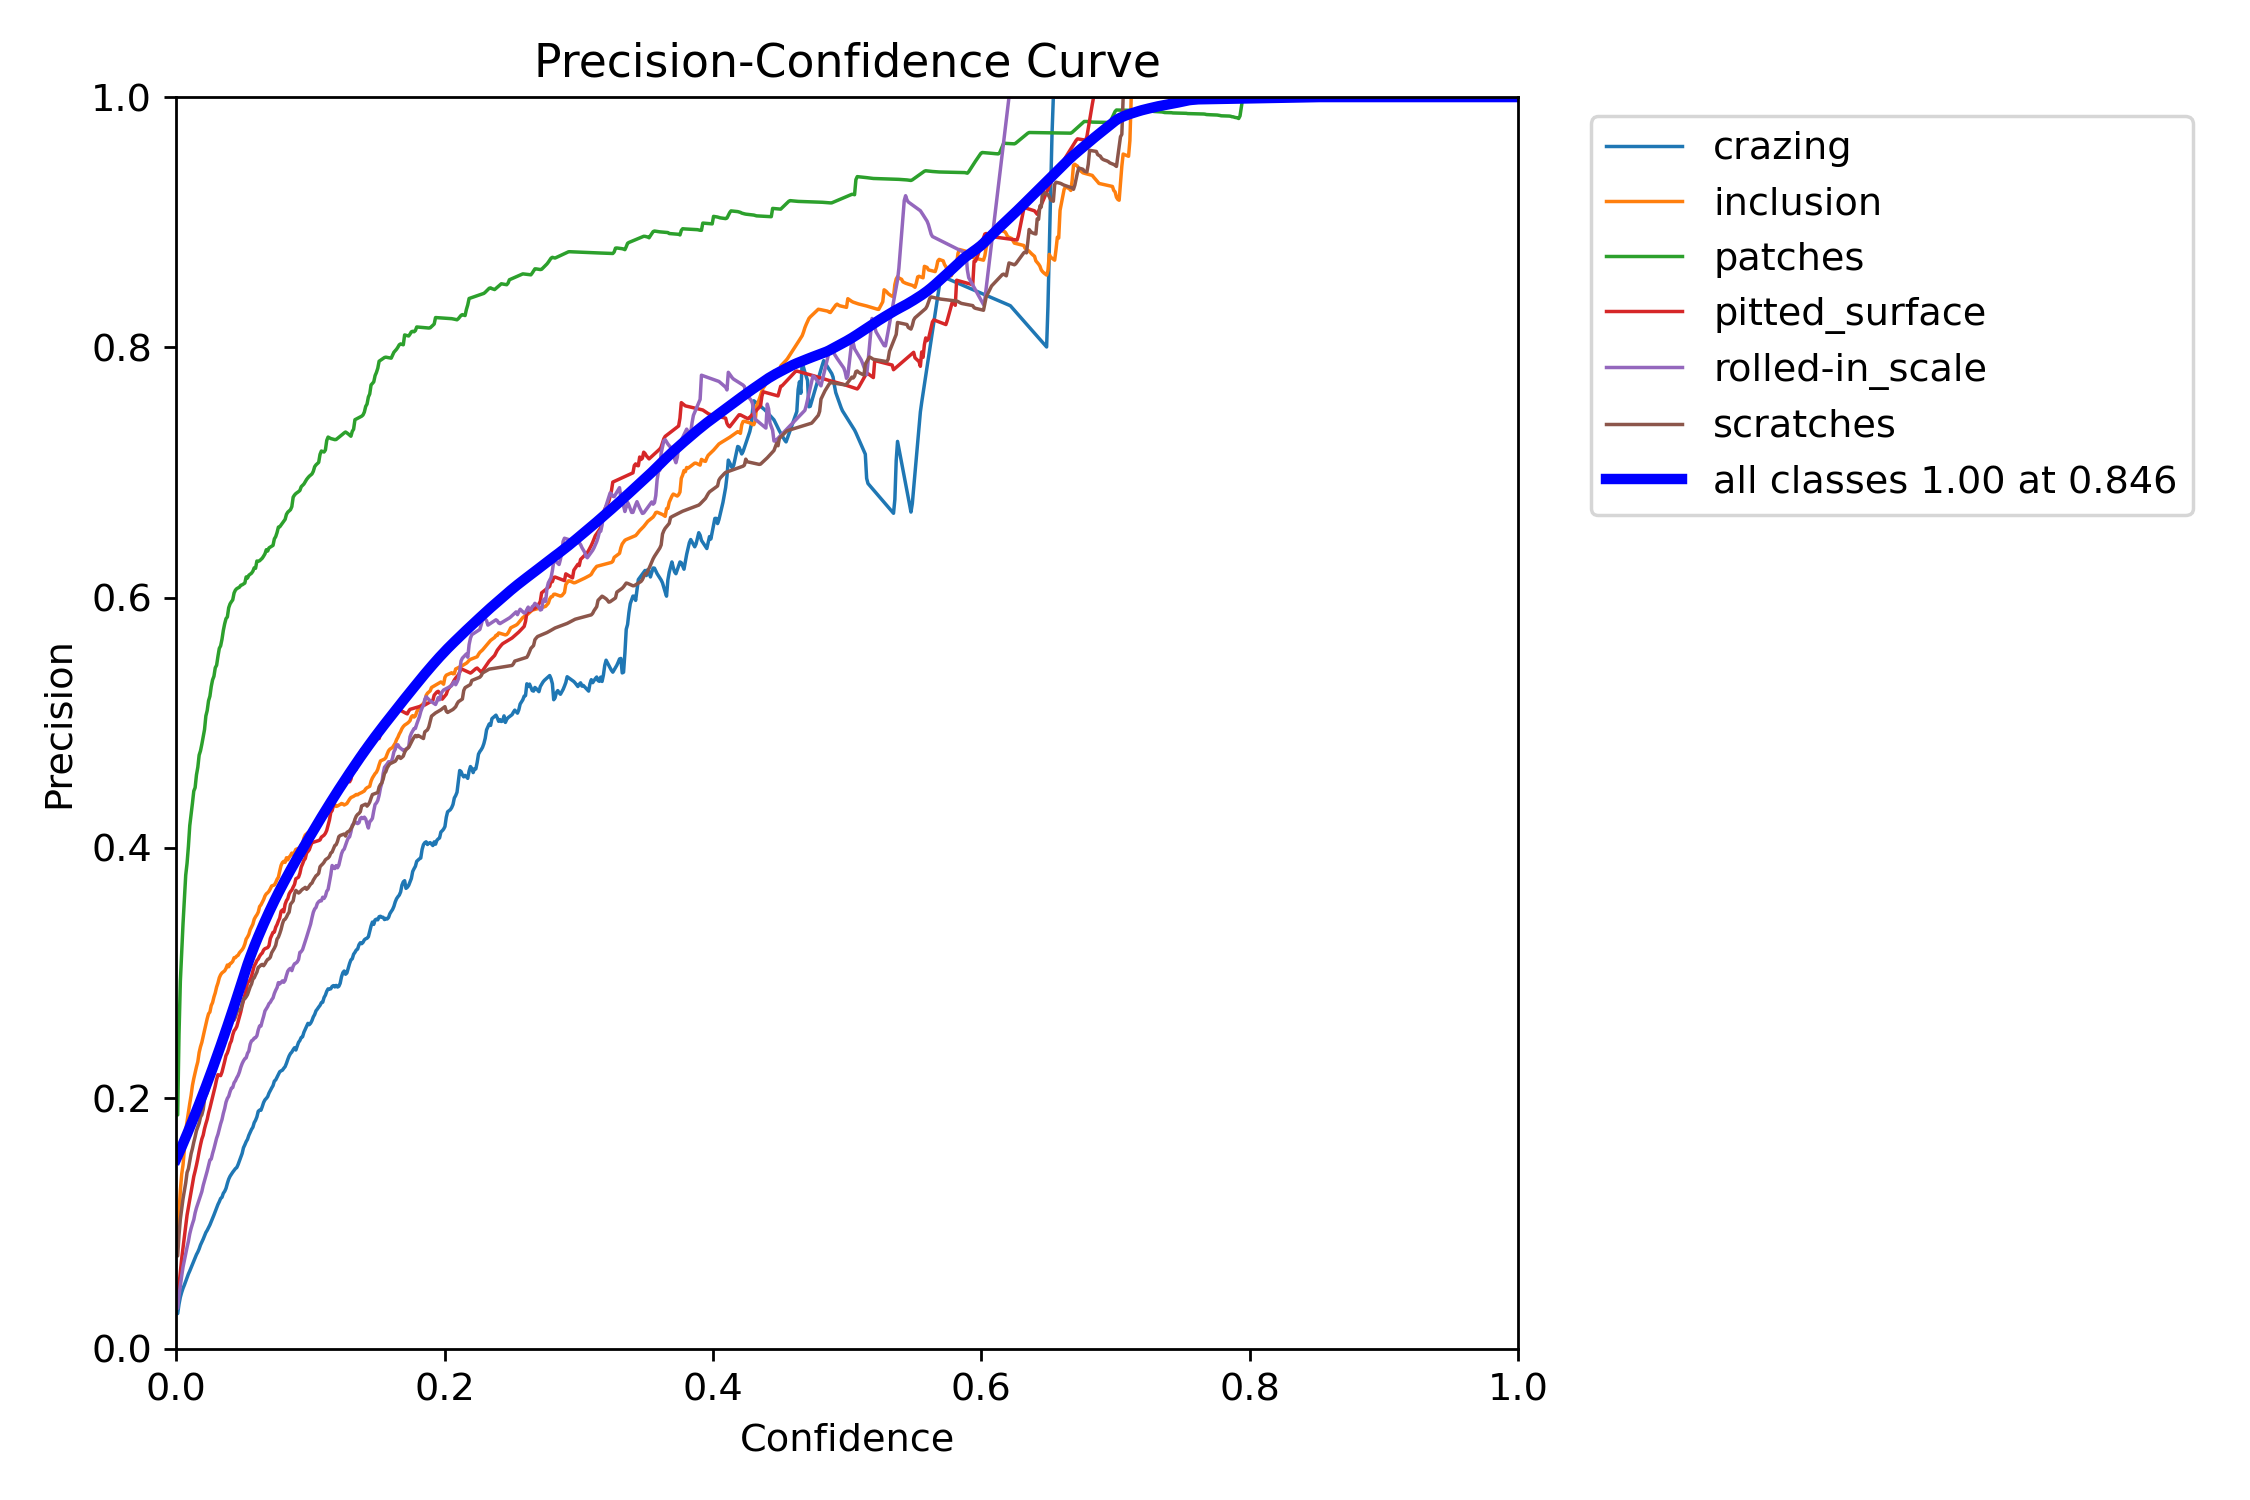
\includegraphics[width=0.45\linewidth]{img/BoxP_curvem.png}
		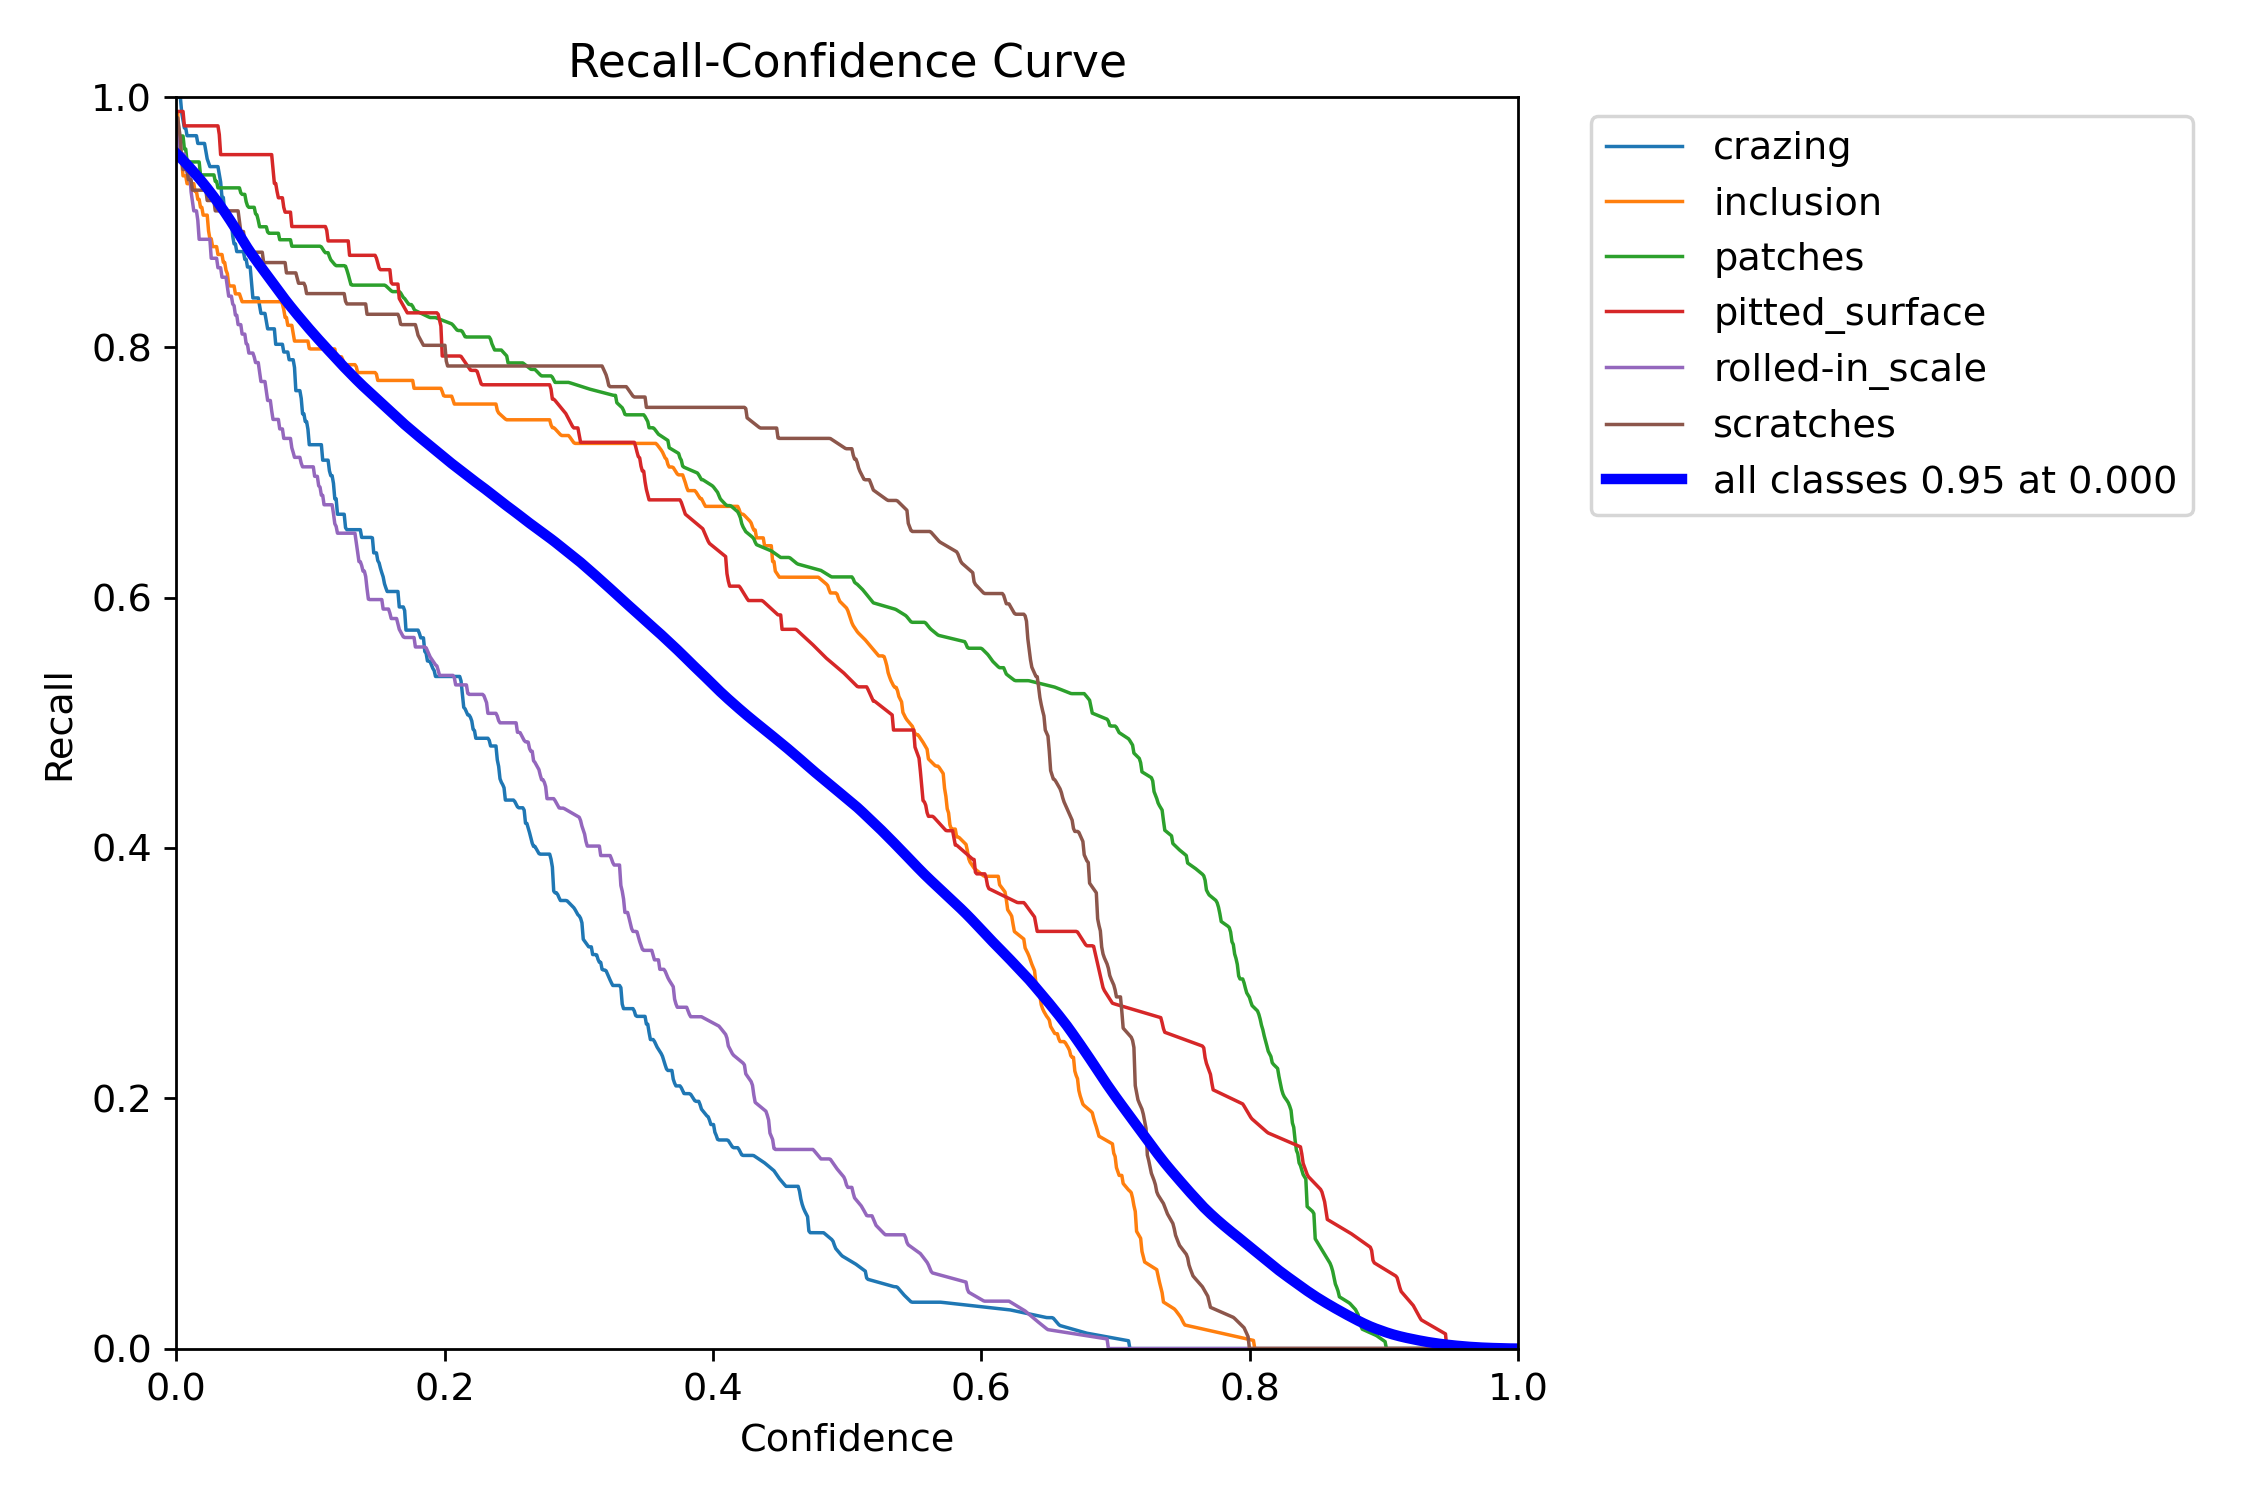
\includegraphics[width=0.45\linewidth]{img/BoxR_curvem.png}
		
		\vspace{0.3cm}
		
		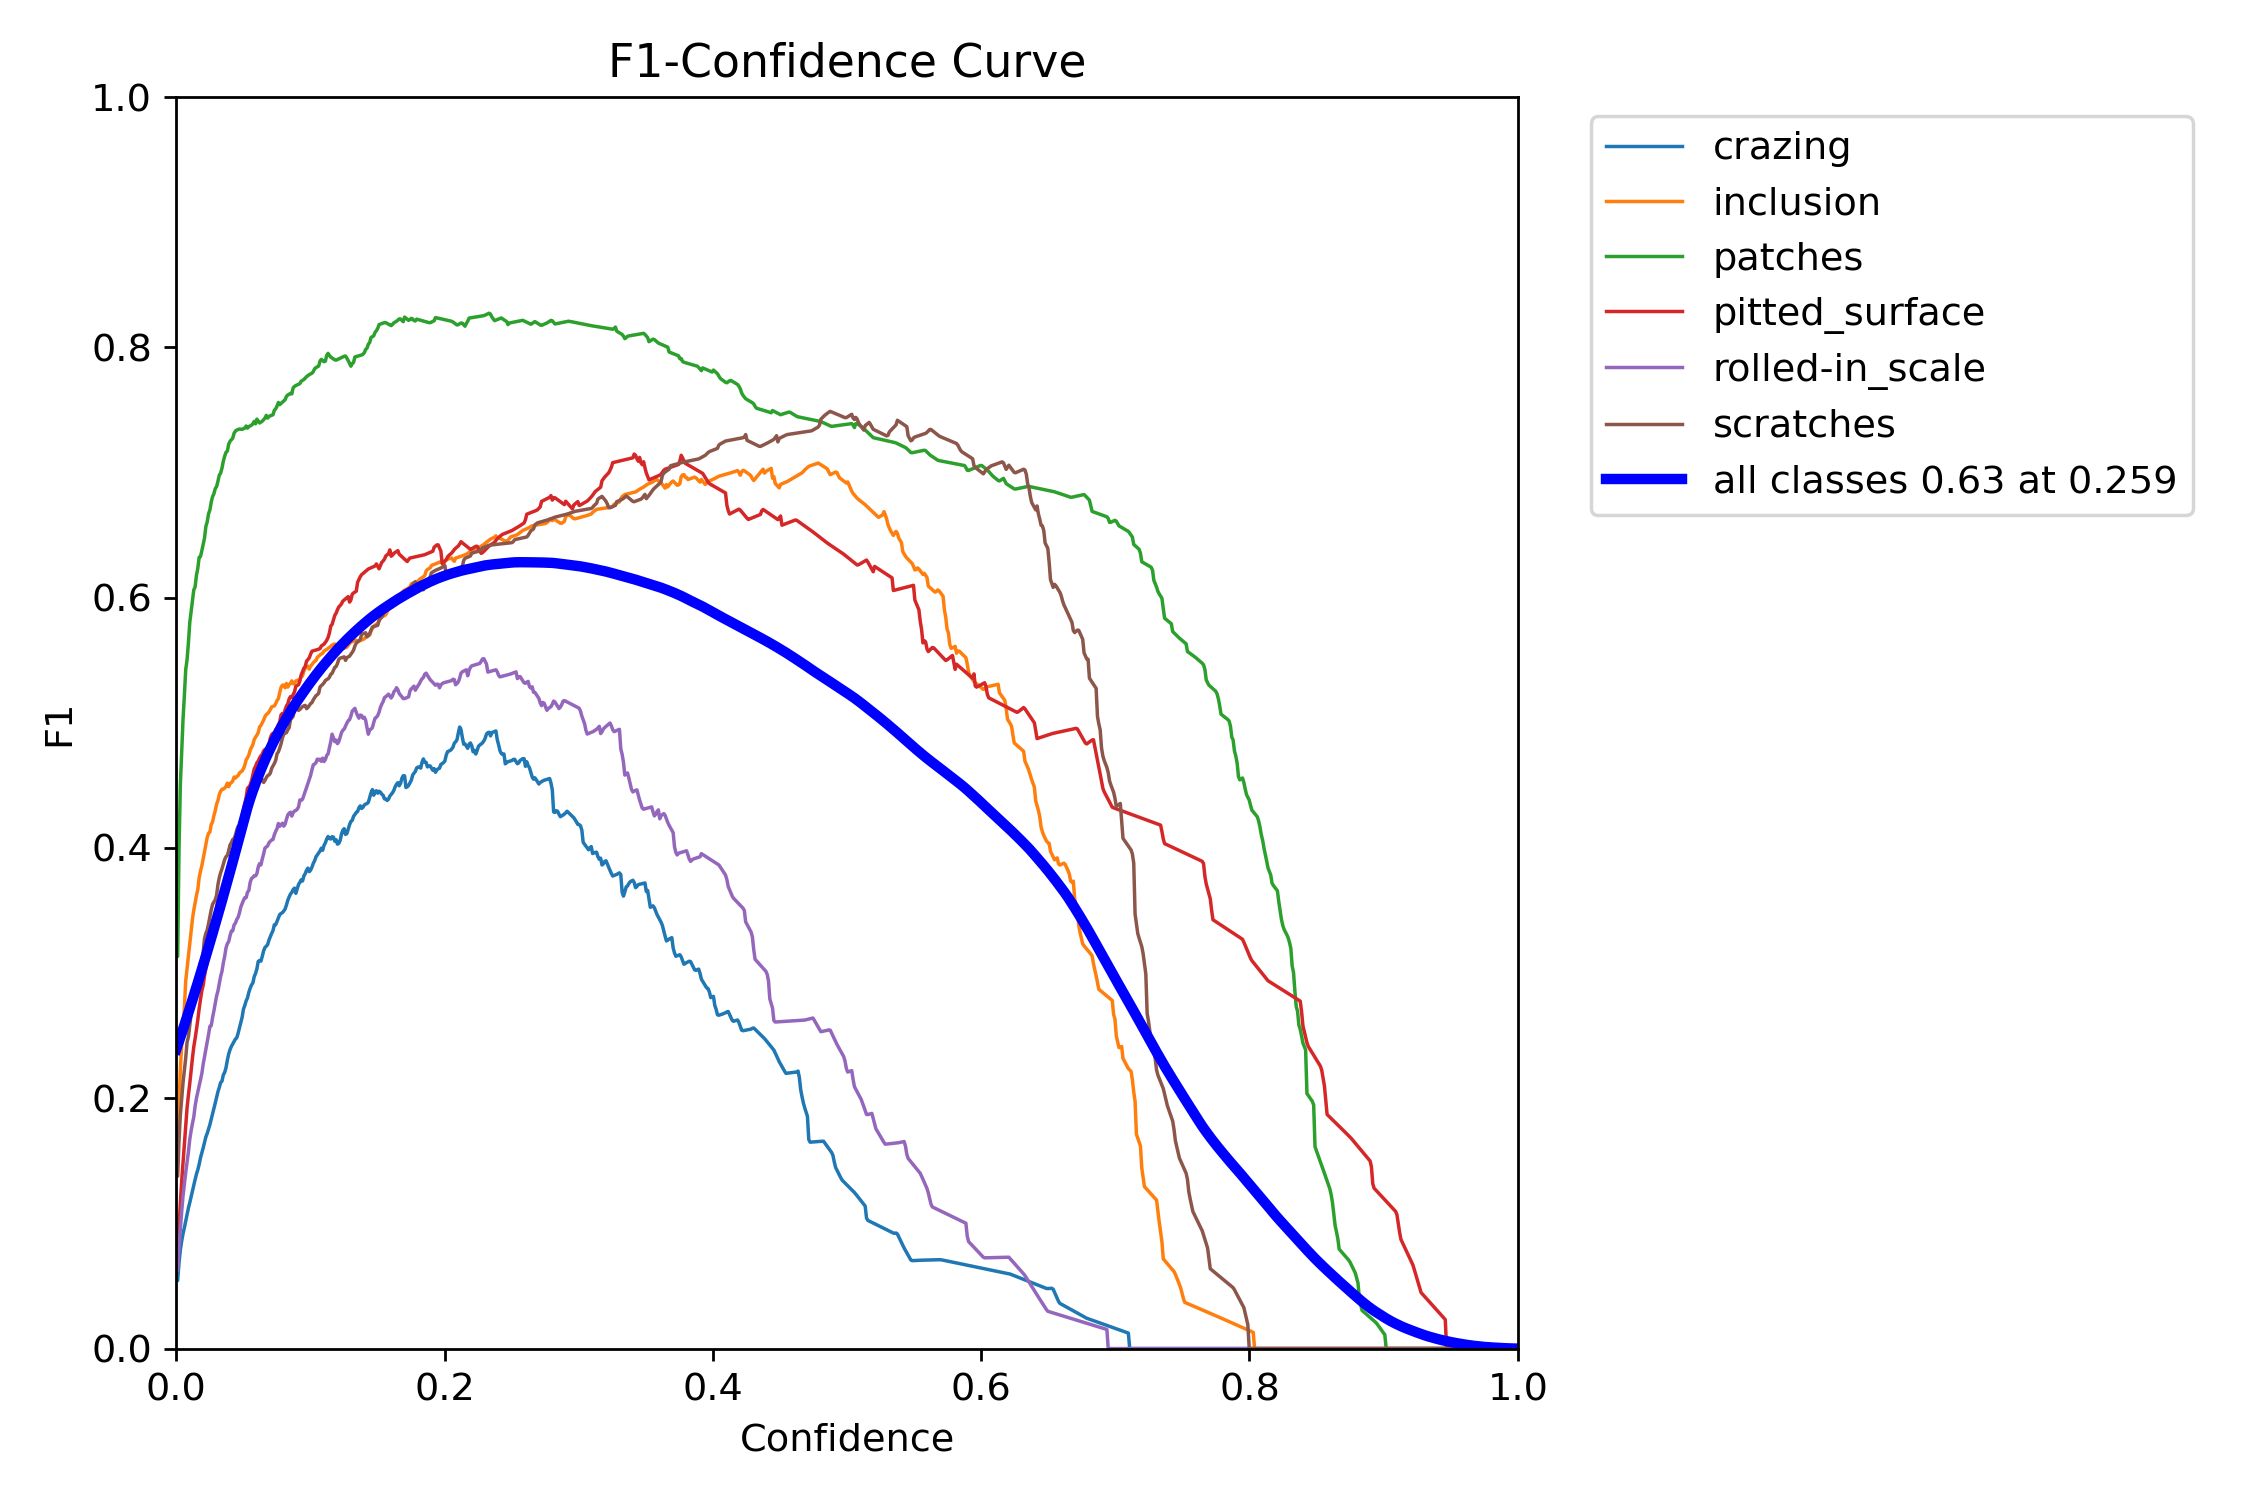
\includegraphics[width=0.45\linewidth]{img/BoxF1_curvem.png}
		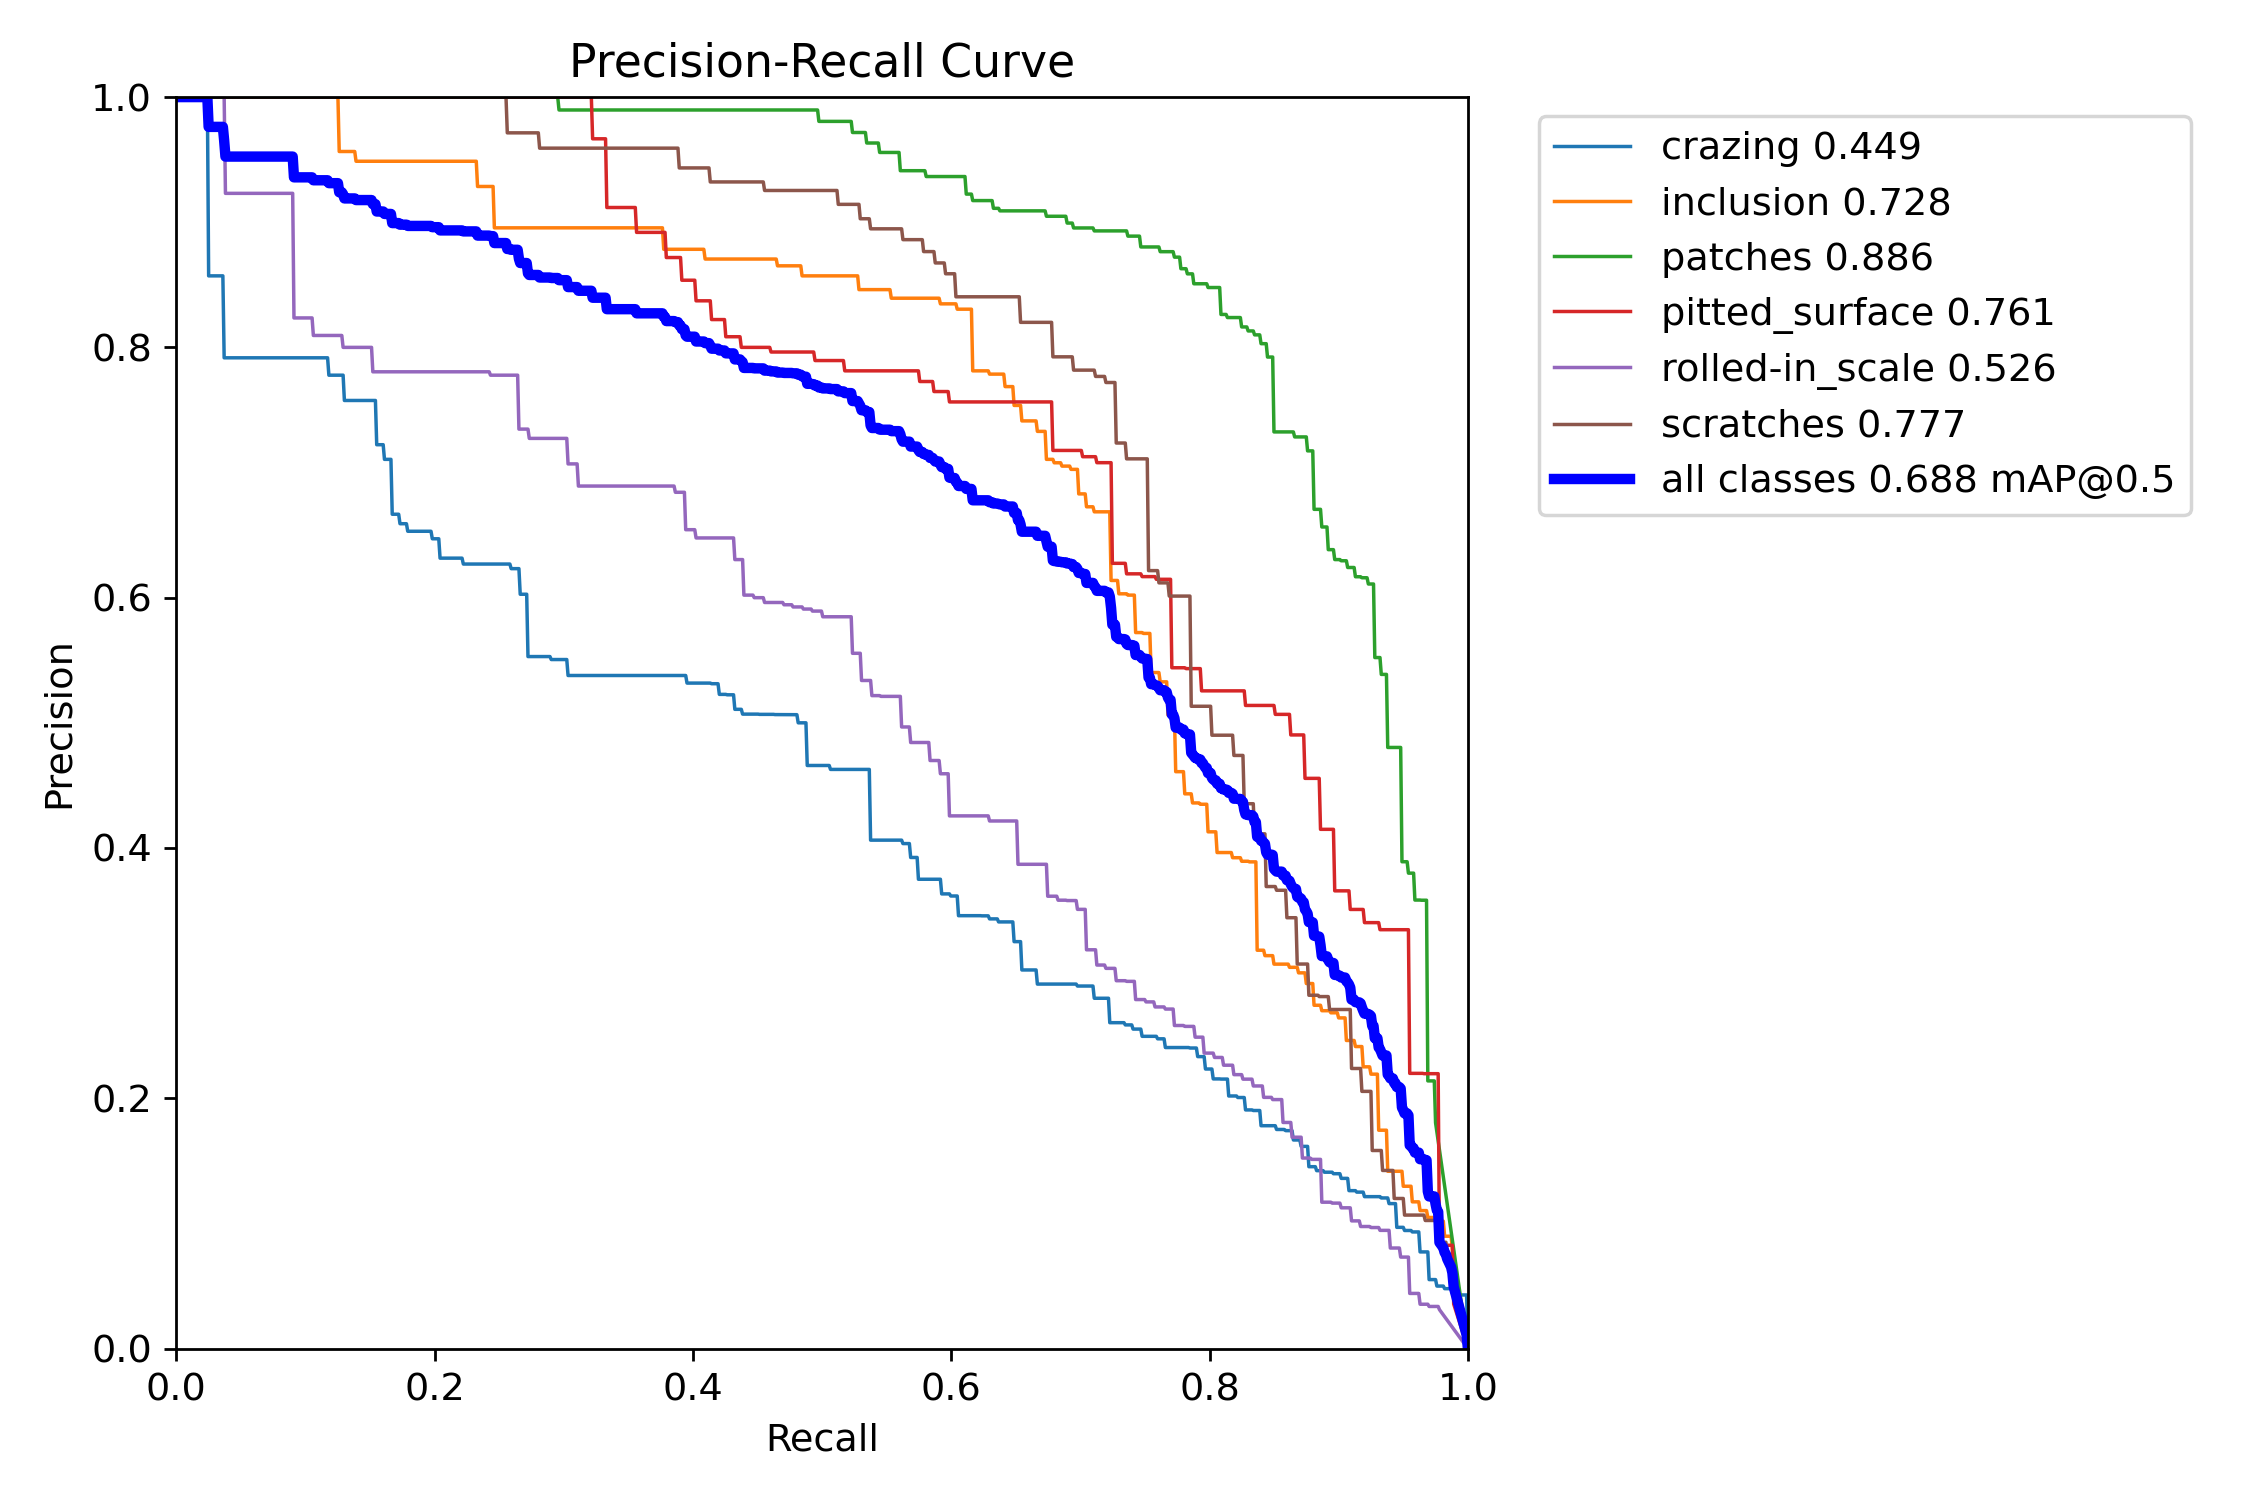
\includegraphics[width=0.45\linewidth]{img/BoxPR_curvem.png}
		\caption{نمودارهای \lr{precision}، \lr{Recall} و \lr{F1score} برحسب مقدار \lr{Confidence} و همچنین نمودار \lr{precision-Recall}}
	\end{figure}
	همانطور که مشاهده می‌شود در کلاس \lr{scrathes}و \lr{crazing} نتایج بهبود داشته است. در برخی کلاس‌ها مقداری نتایج افت داشته است ولی به صورت برآیندی نتایج بهتر شده است. در نمودارهای روند آموزش اورفیت مشاهده نمی‌شود و مدل به شکل مناسبی آموزش دیده است.
	
	اندک بهبودی که مدل ایجاد کرده قابل تقدیر است اما بار محاسباتی را شدیدا بالابرده است بطوریکه تعداد پارامتر آموزش دیده 7 برابر شده است.
	
	در کل عملکرد این مدل بهتر از مدل‌های قبلی است و بین دو مدل قبل آنچنان تفاوتی نیست و بنظر می‌آید که مدل اولی در یکسری از کلاس‌ها عملکرد بهتری داشته که به چشم می‌آید اما مدل دوم در آنها خوب نبوده برعکس مدل دوم در بعضی کلاس‌ها مقداری بهبود داشته است.
	
	ماتریس درهمریختگی مربوط به این مدل نیز به صورت زیر است:
	\begin{figure}[H]
		\centering
		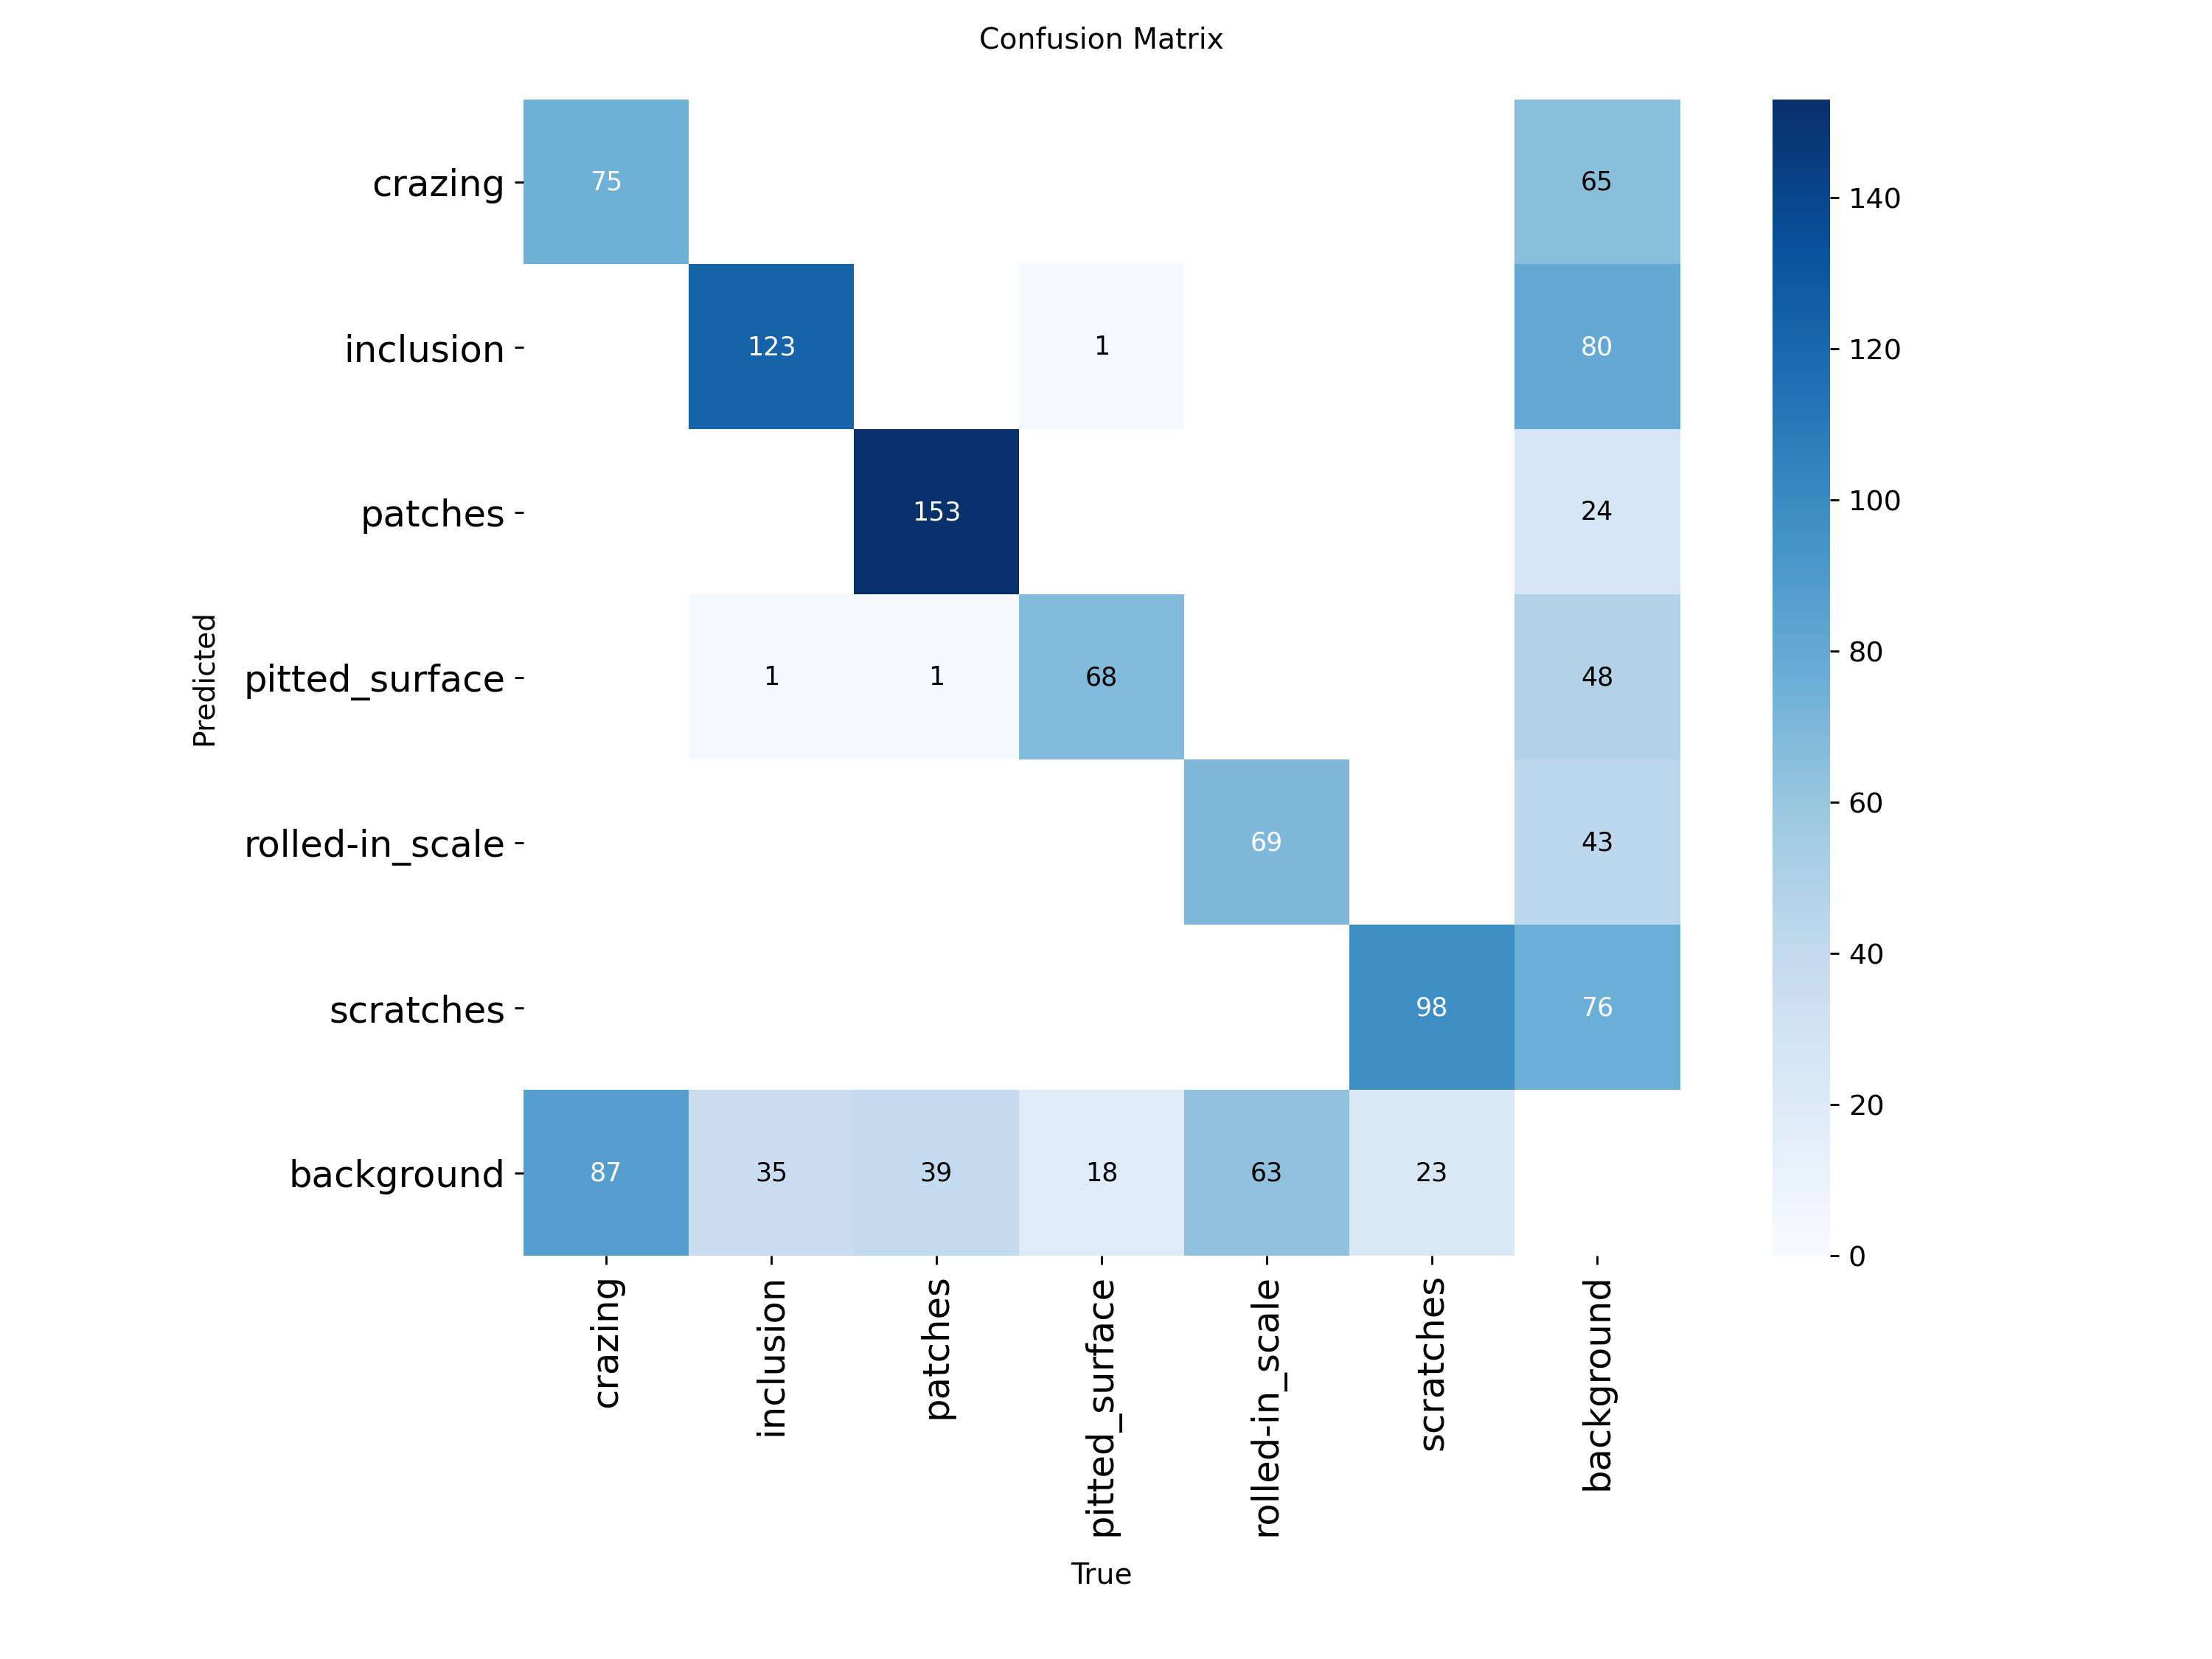
\includegraphics[width=0.3\linewidth]{img/confusion_matrixm.png}
		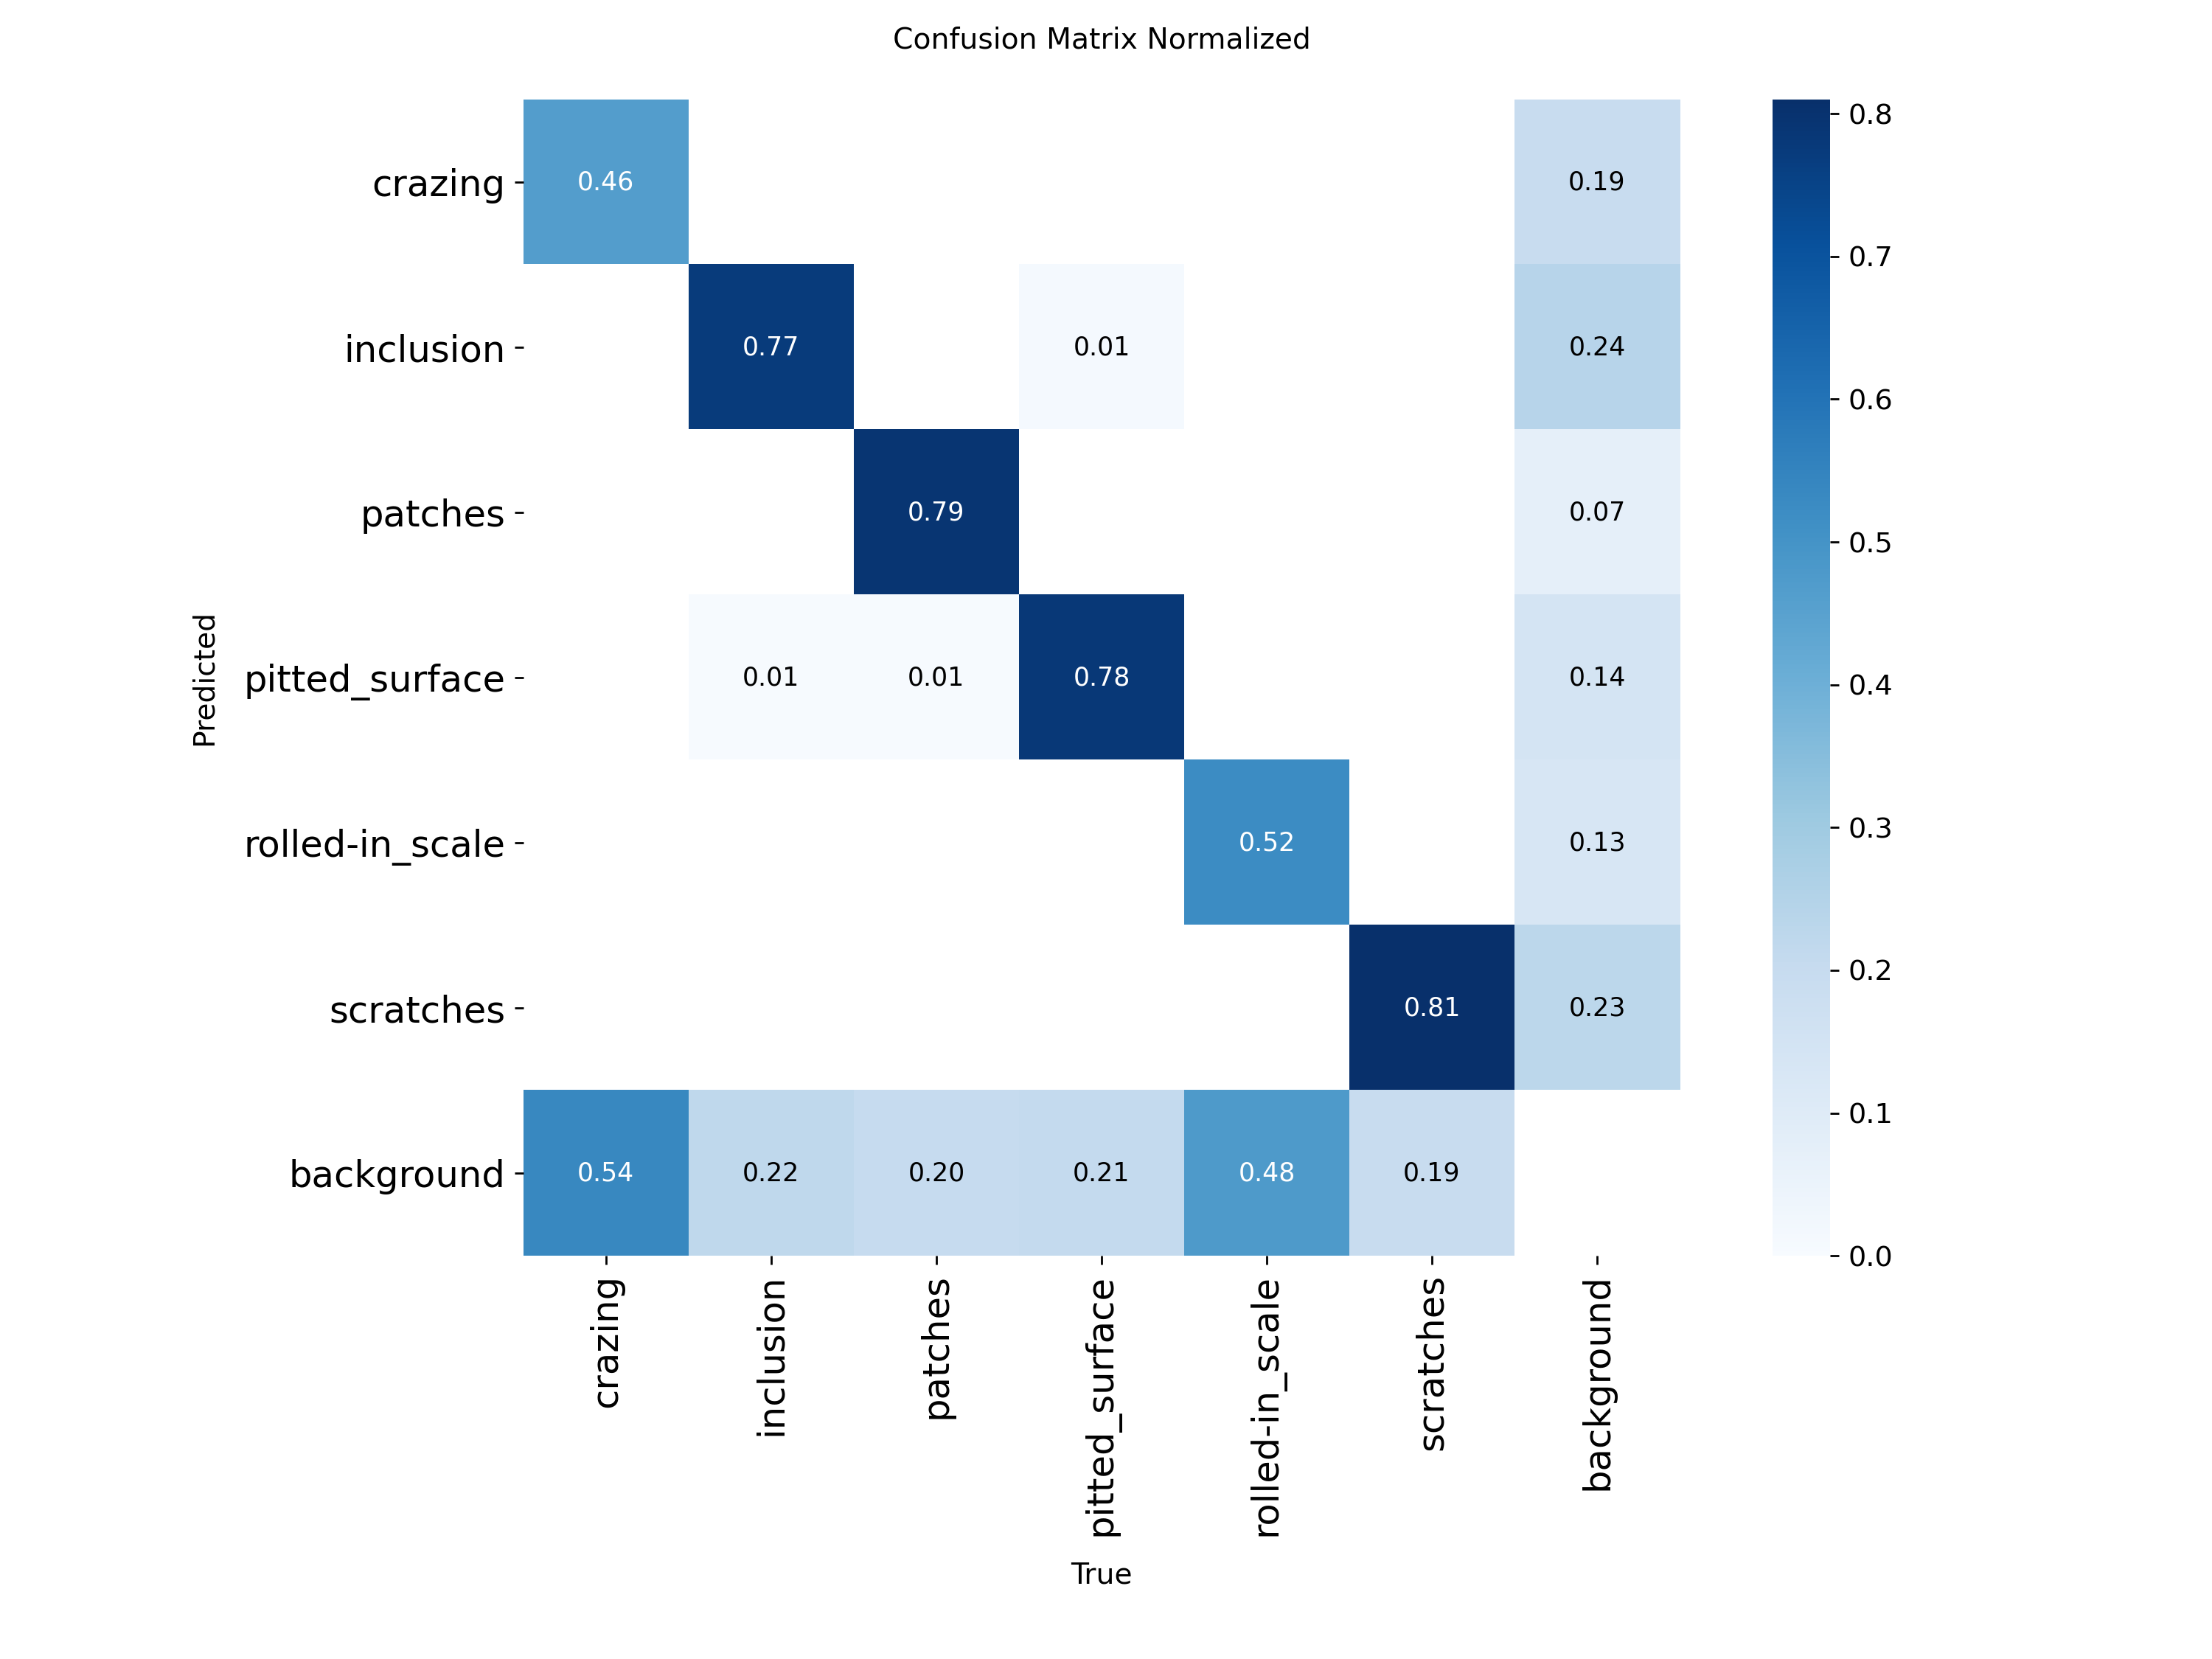
\includegraphics[width=0.3\linewidth]{img/confusion_matrix_normalizedm.png}
		\caption{ماتریس درهمریختگی}
	\end{figure}
	
	همانطور که مشاهده می‌شود تشخیص مدل در کلاس‌ها بهتر شده و کمتر تشخیص غلط بر روی پس زمینه دارد.
	
	
	نمونه خروجی گرفته شده از این مدل نیز به صورت زیر است:
	\begin{figure}[H]
		\centering
		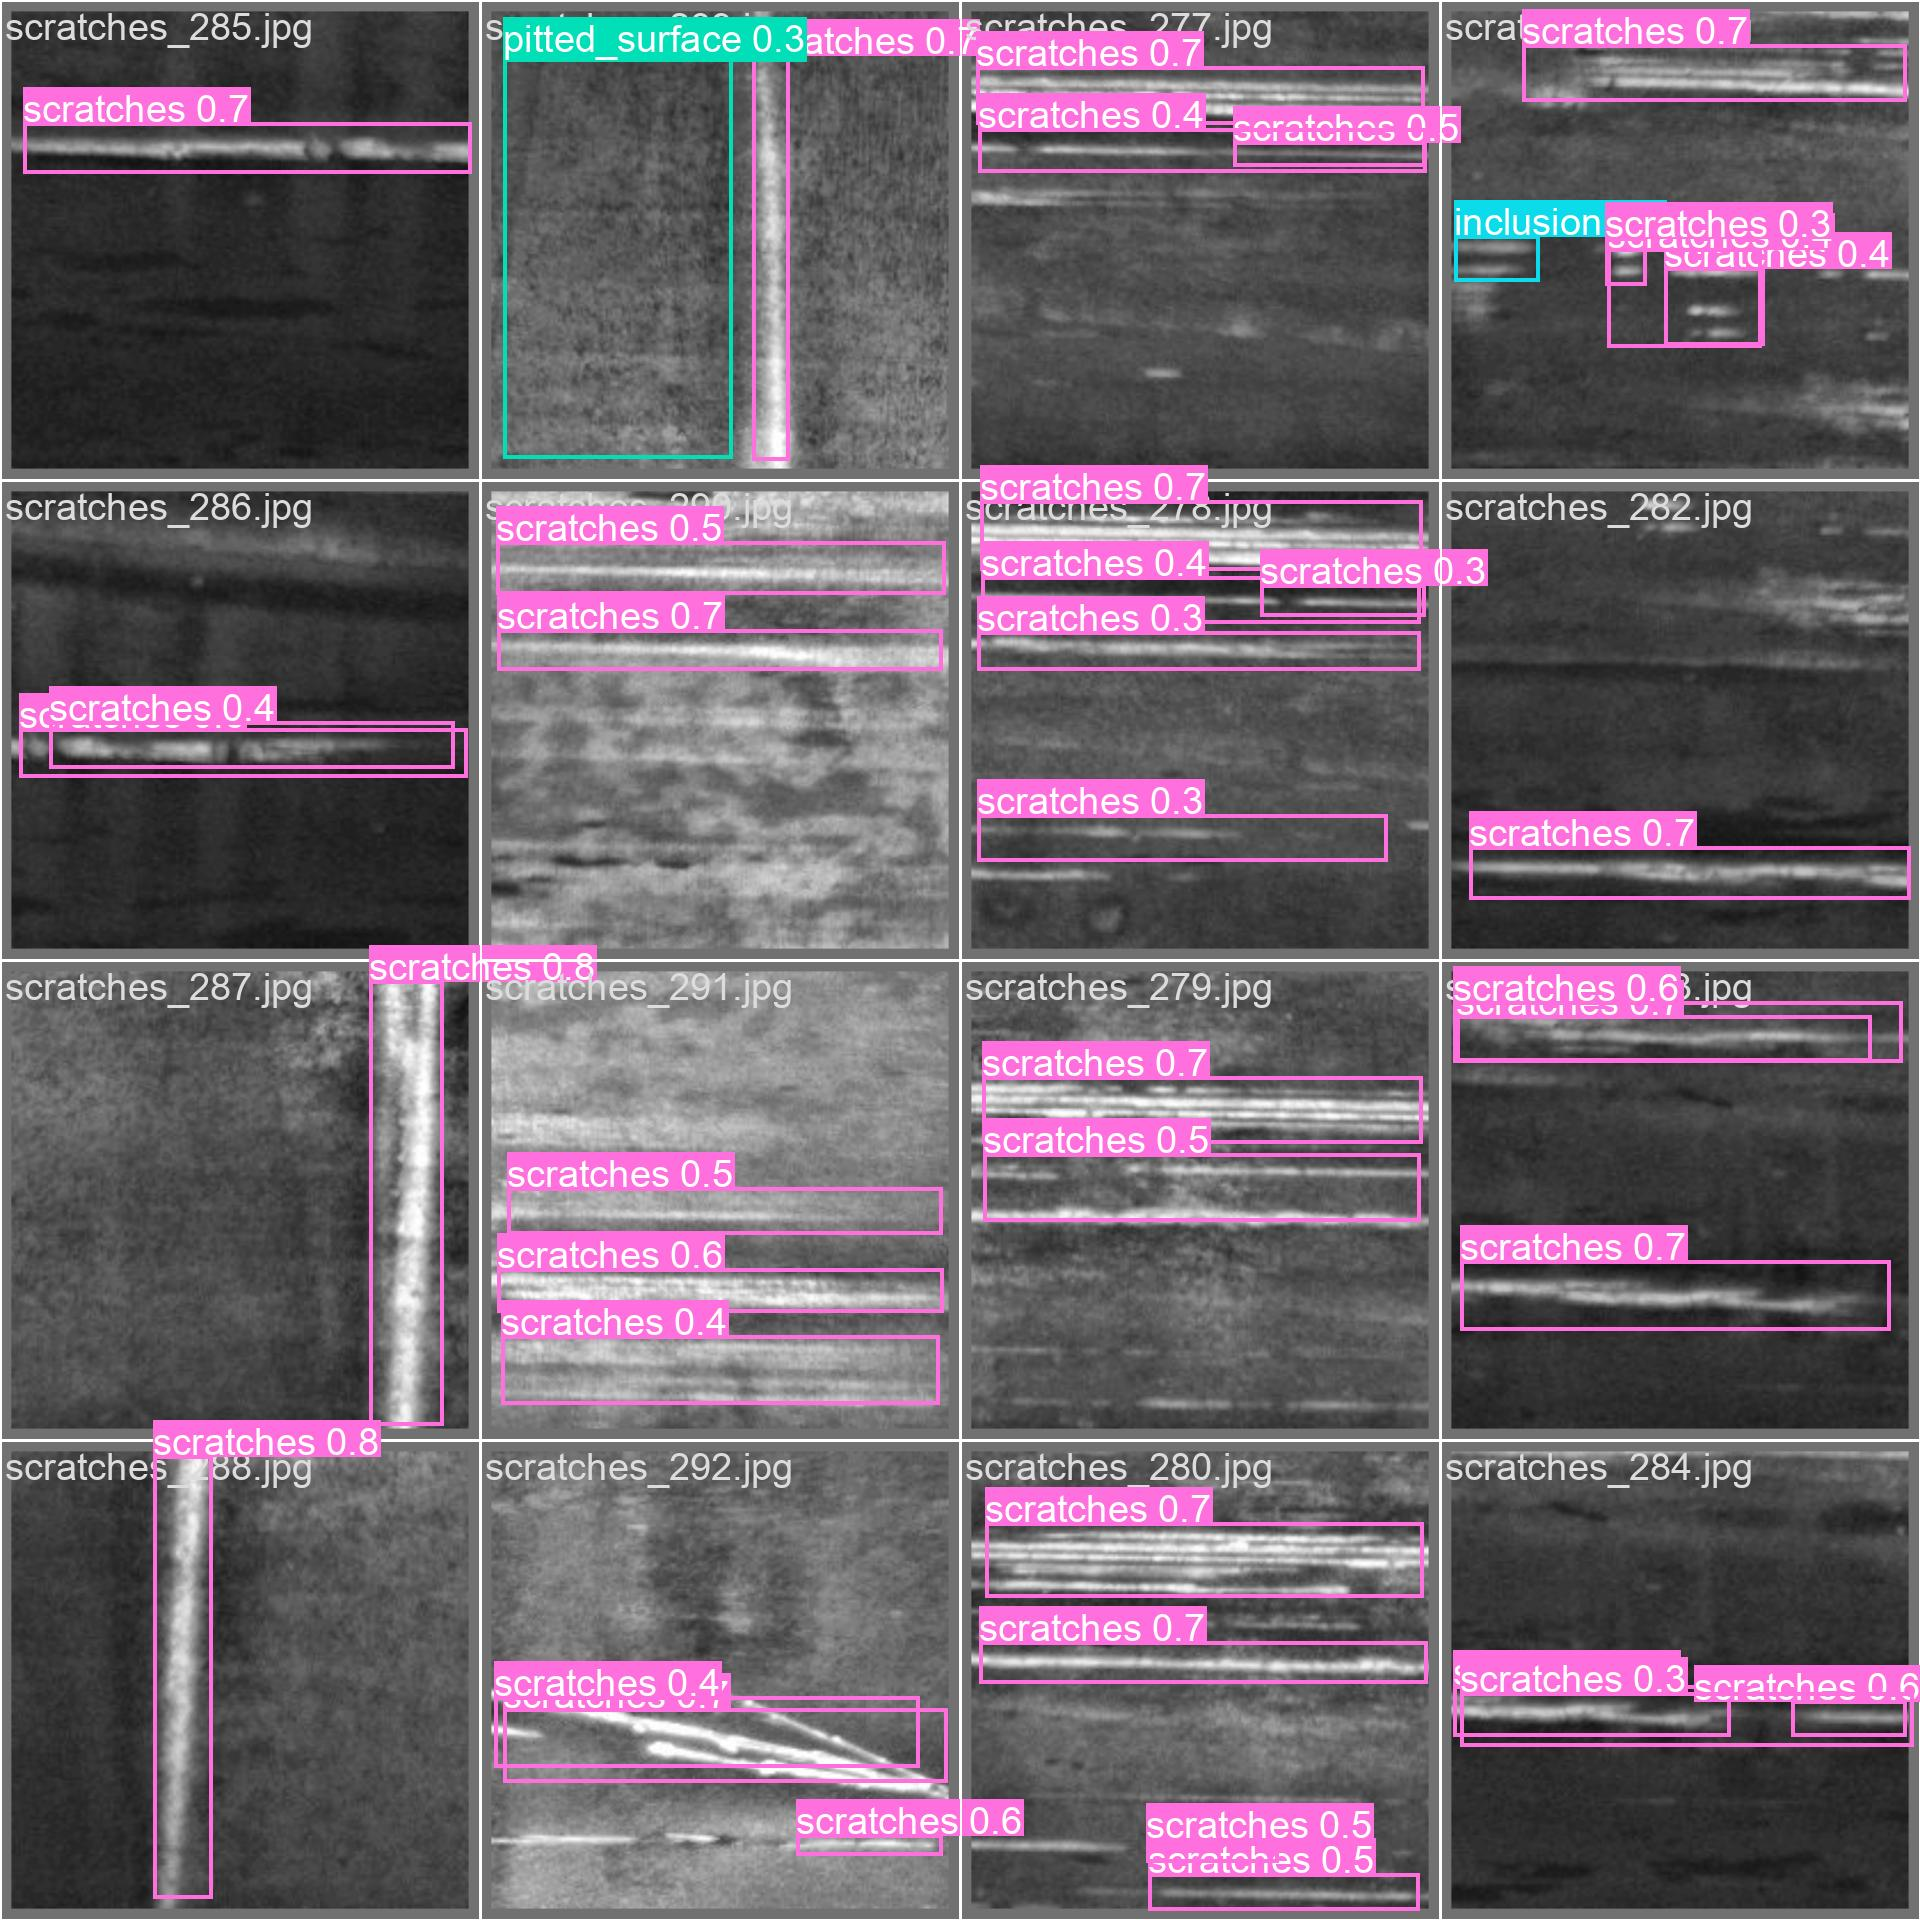
\includegraphics[width=0.2\linewidth]{img/val_batch0_predm.jpg}
		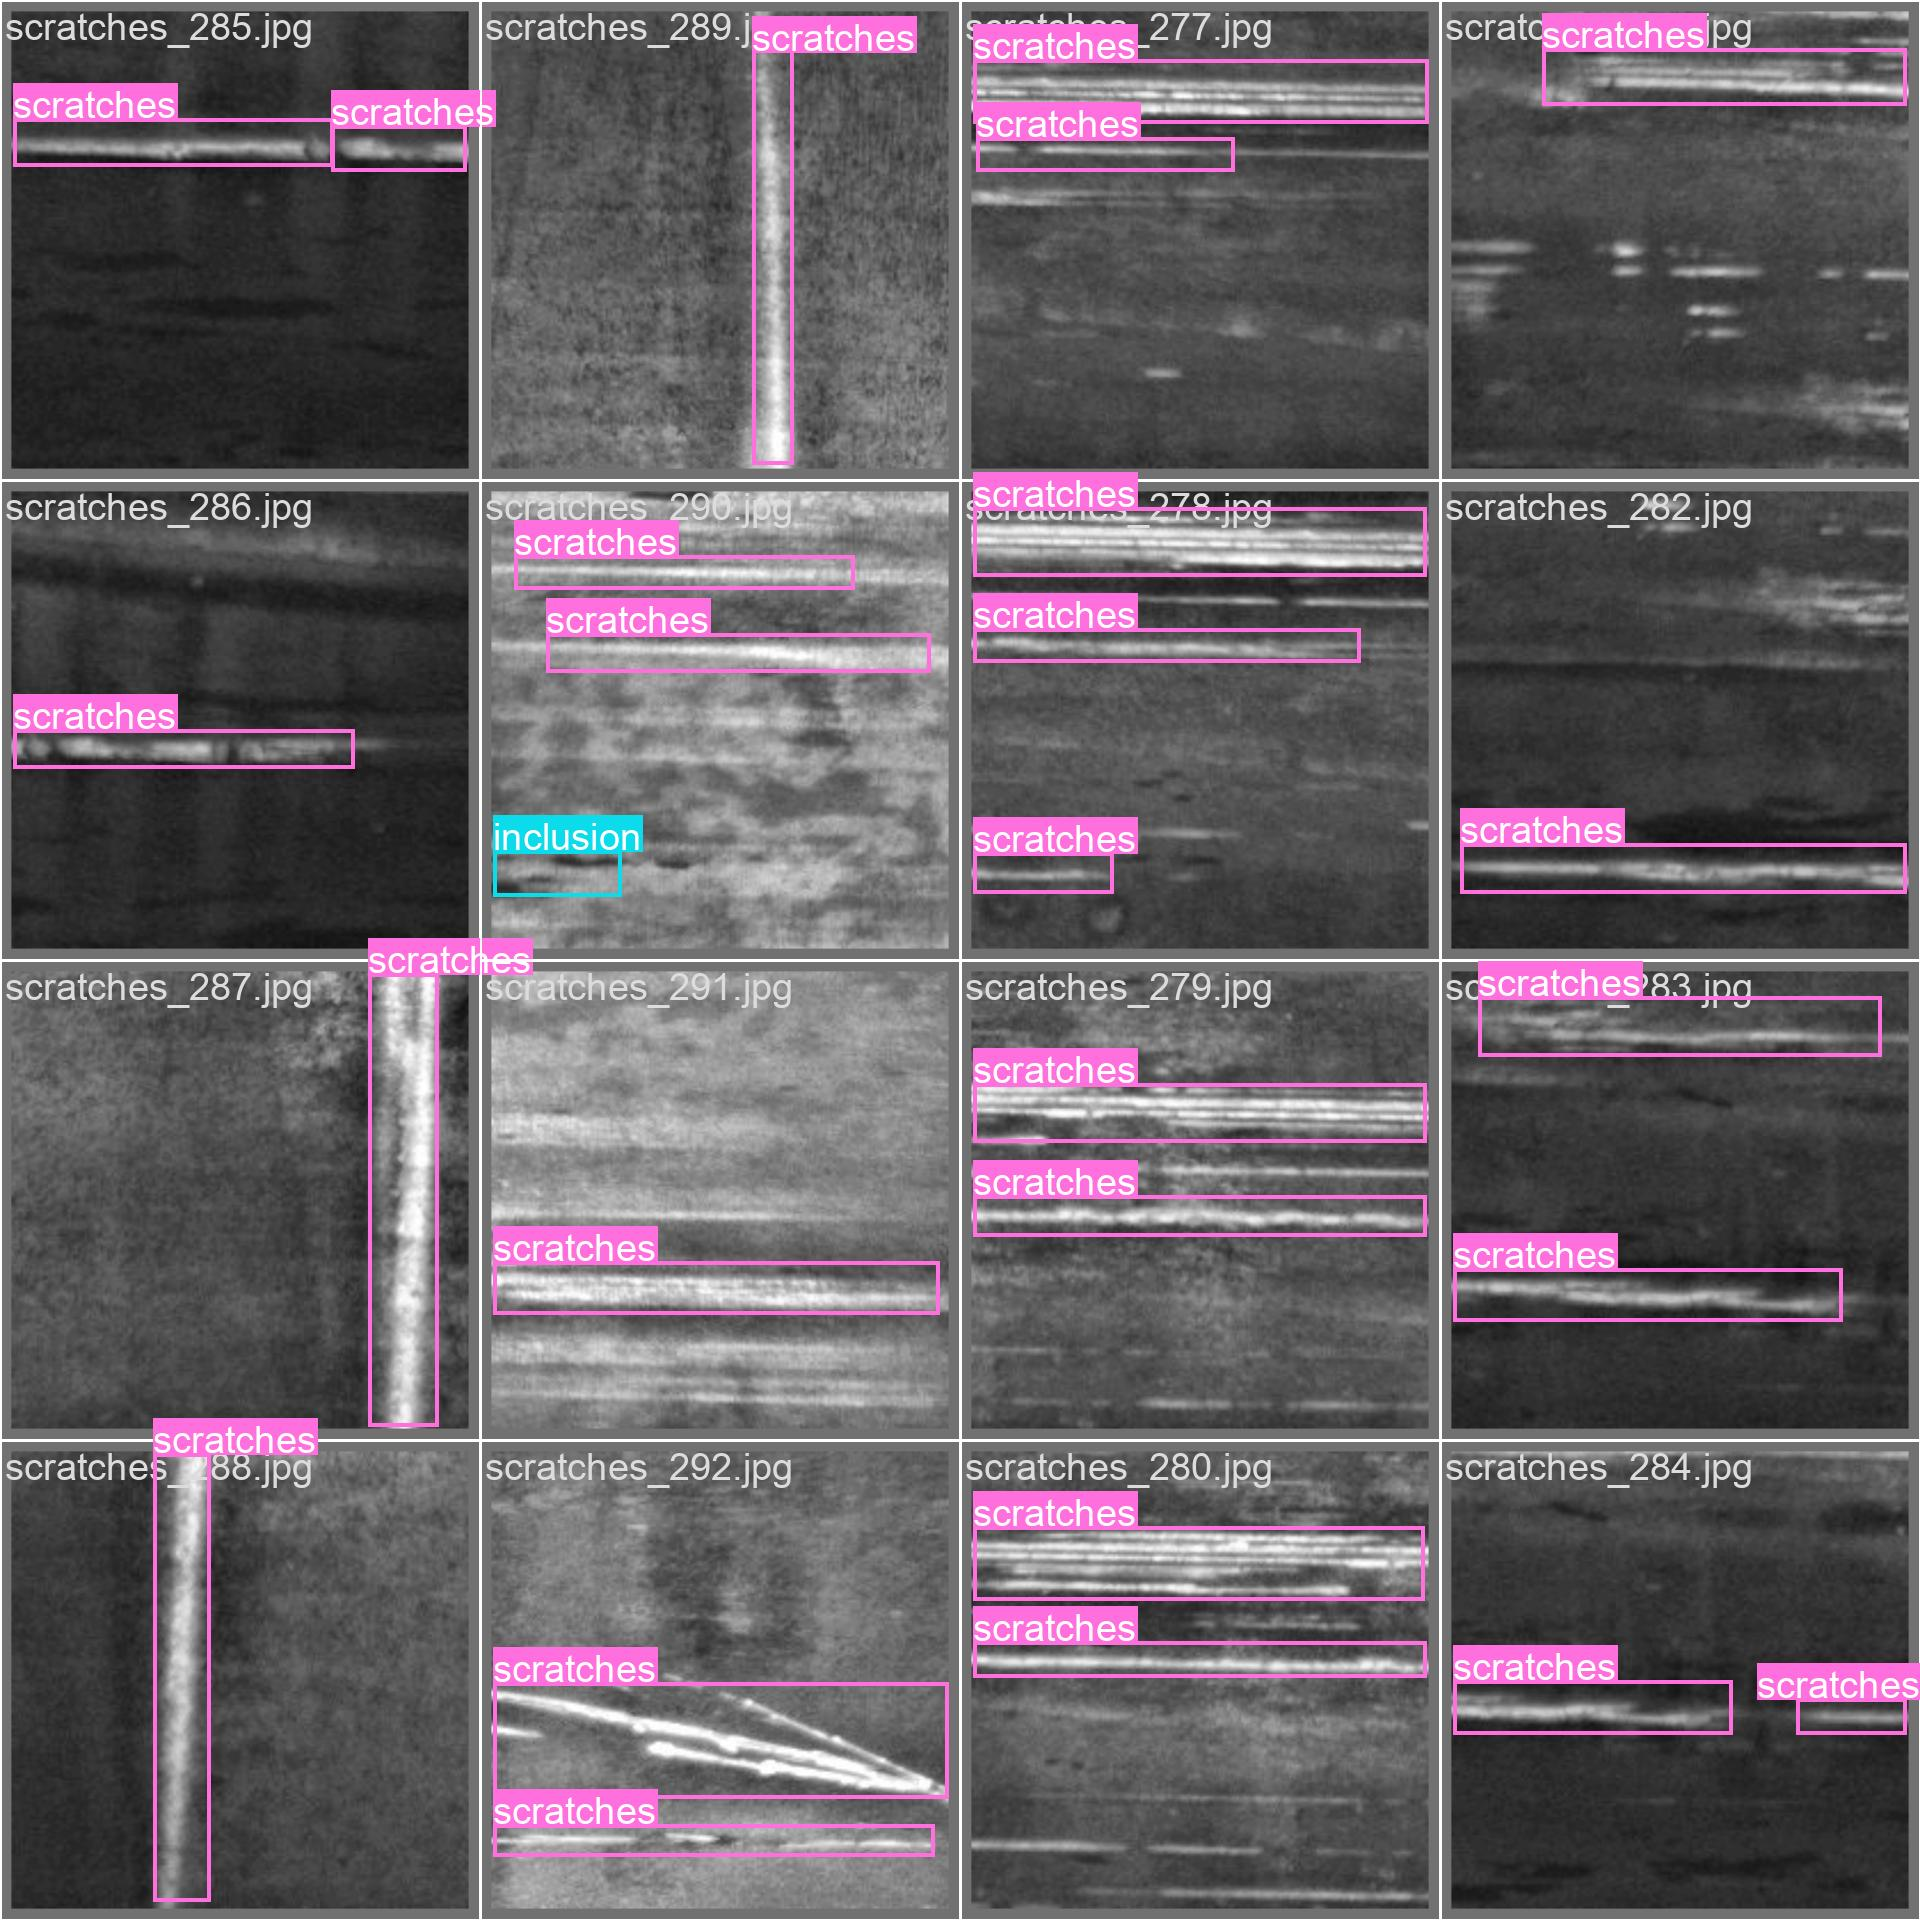
\includegraphics[width=0.2\linewidth]{img/val_batch0_labelsm.jpg}
		
		\vspace{0.3cm}
		
		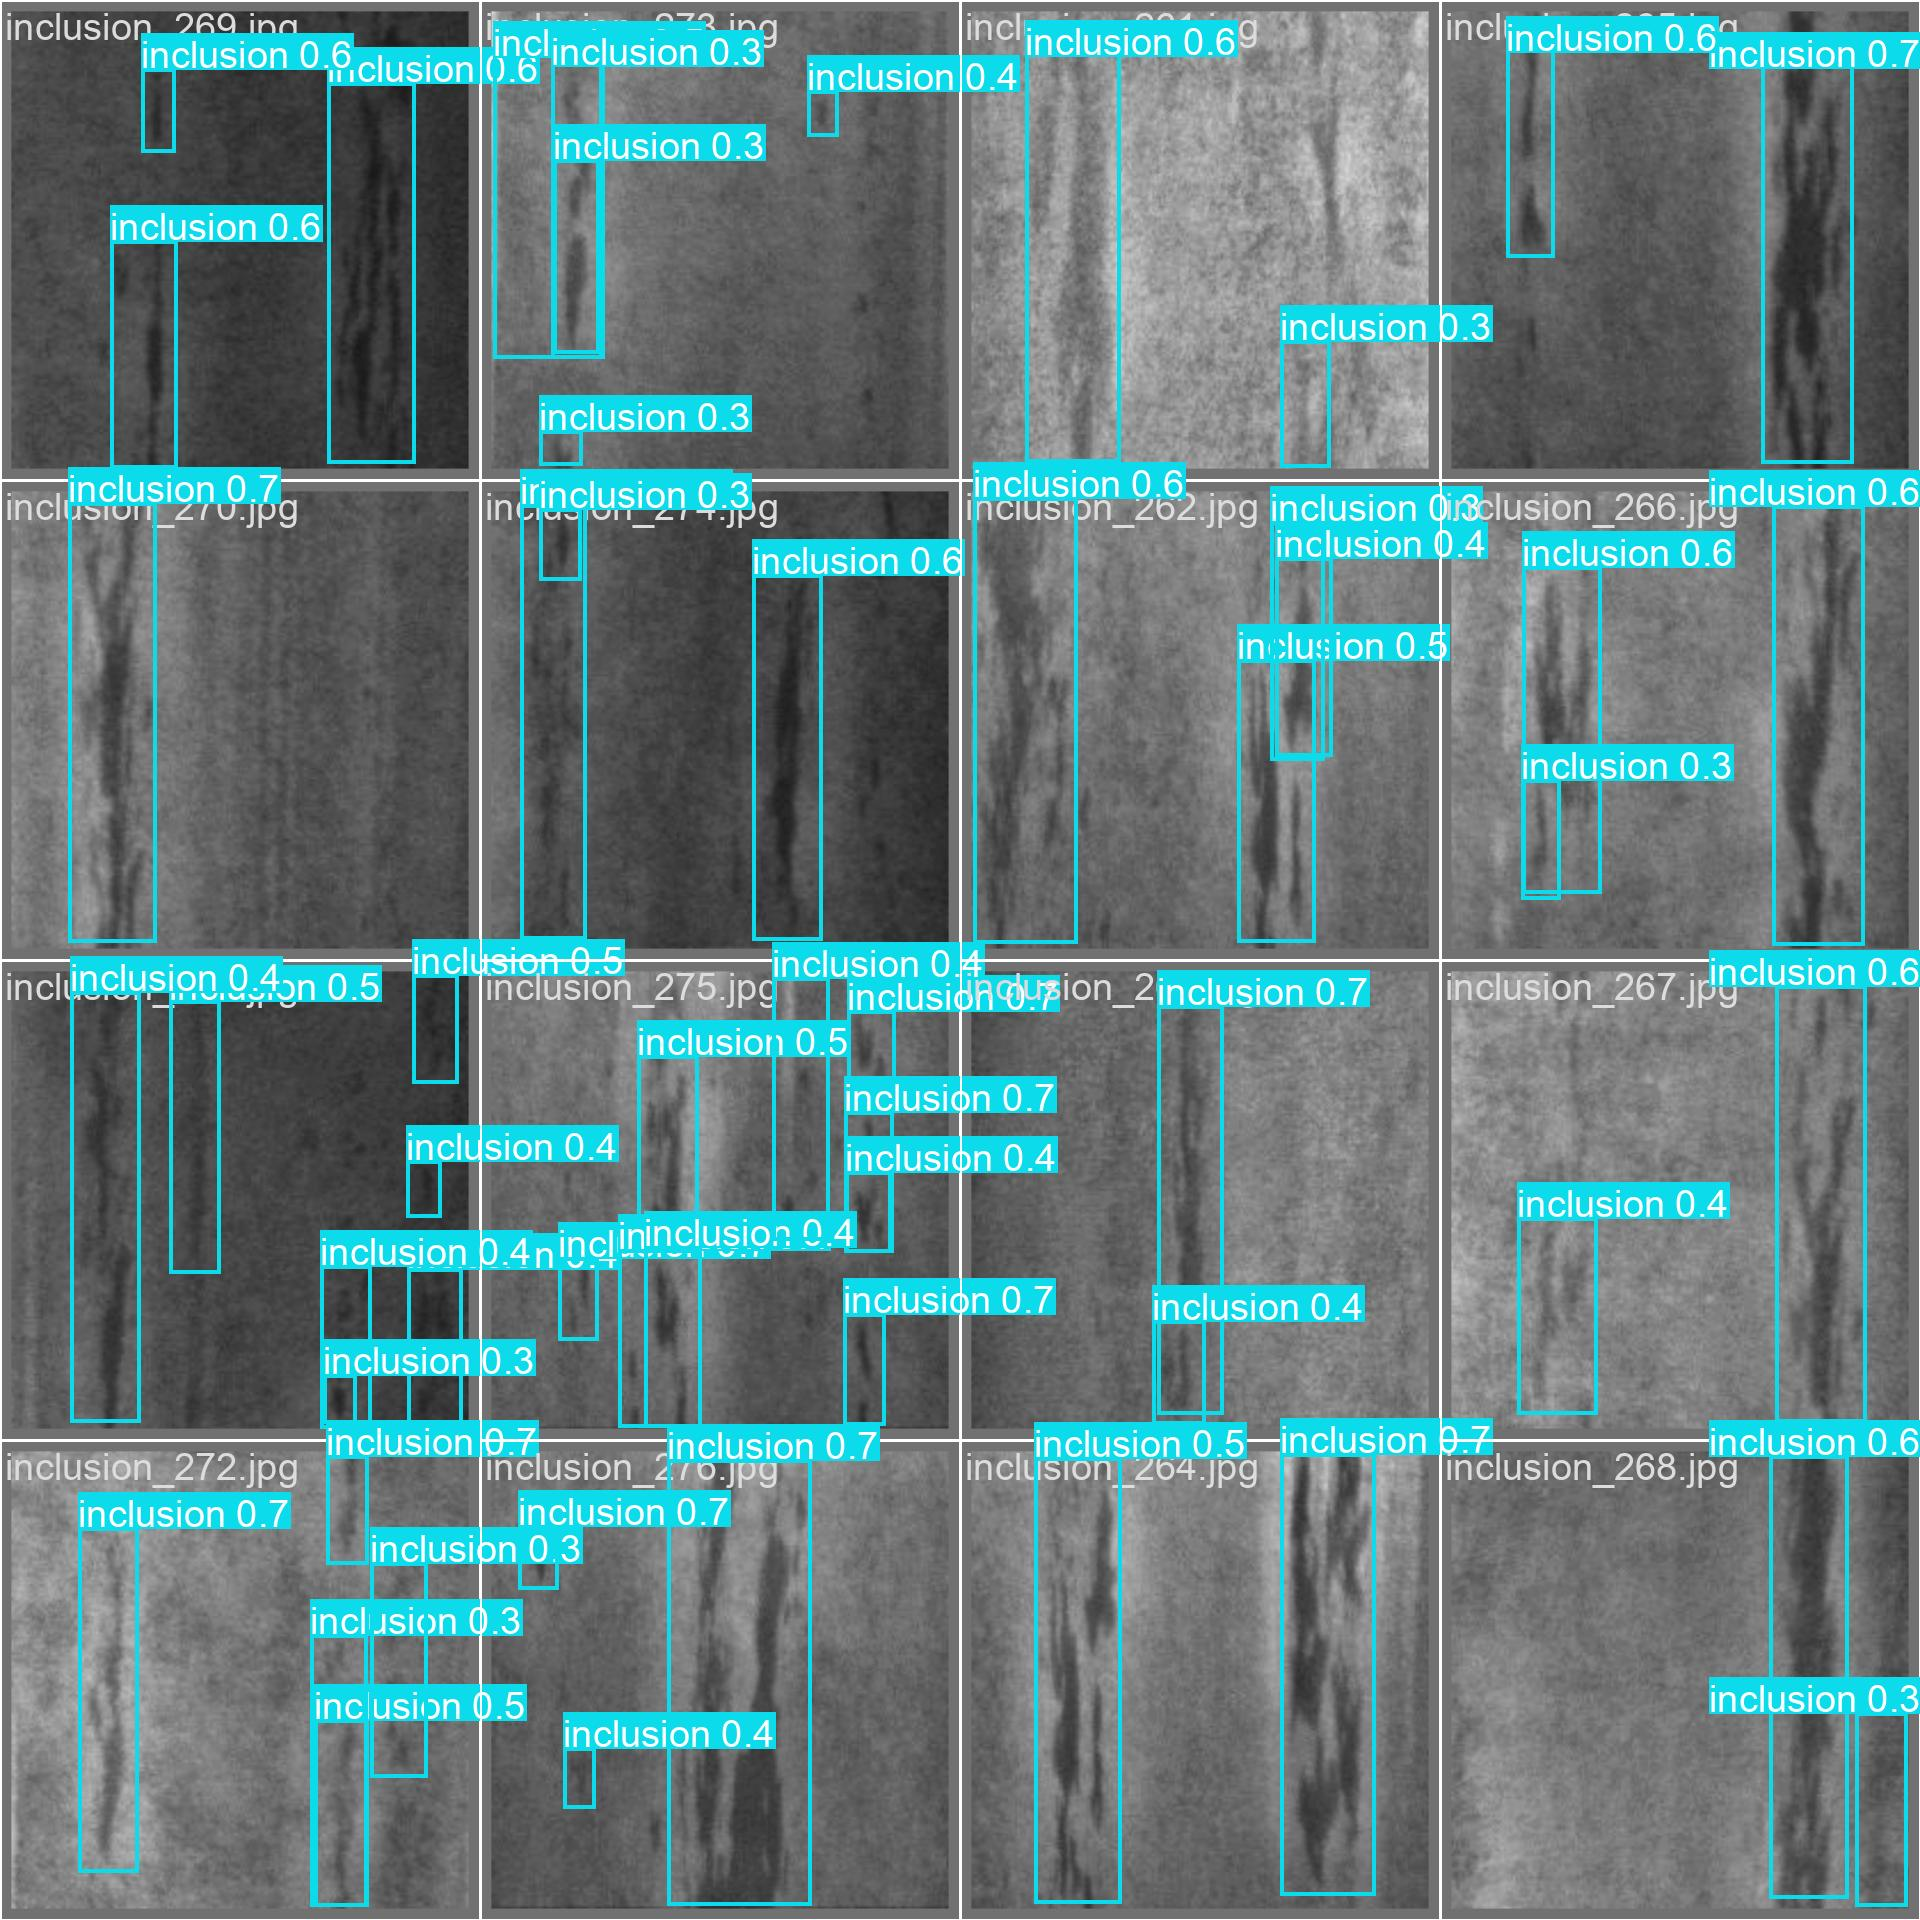
\includegraphics[width=0.2\linewidth]{img/val_batch2_predm.jpg}
		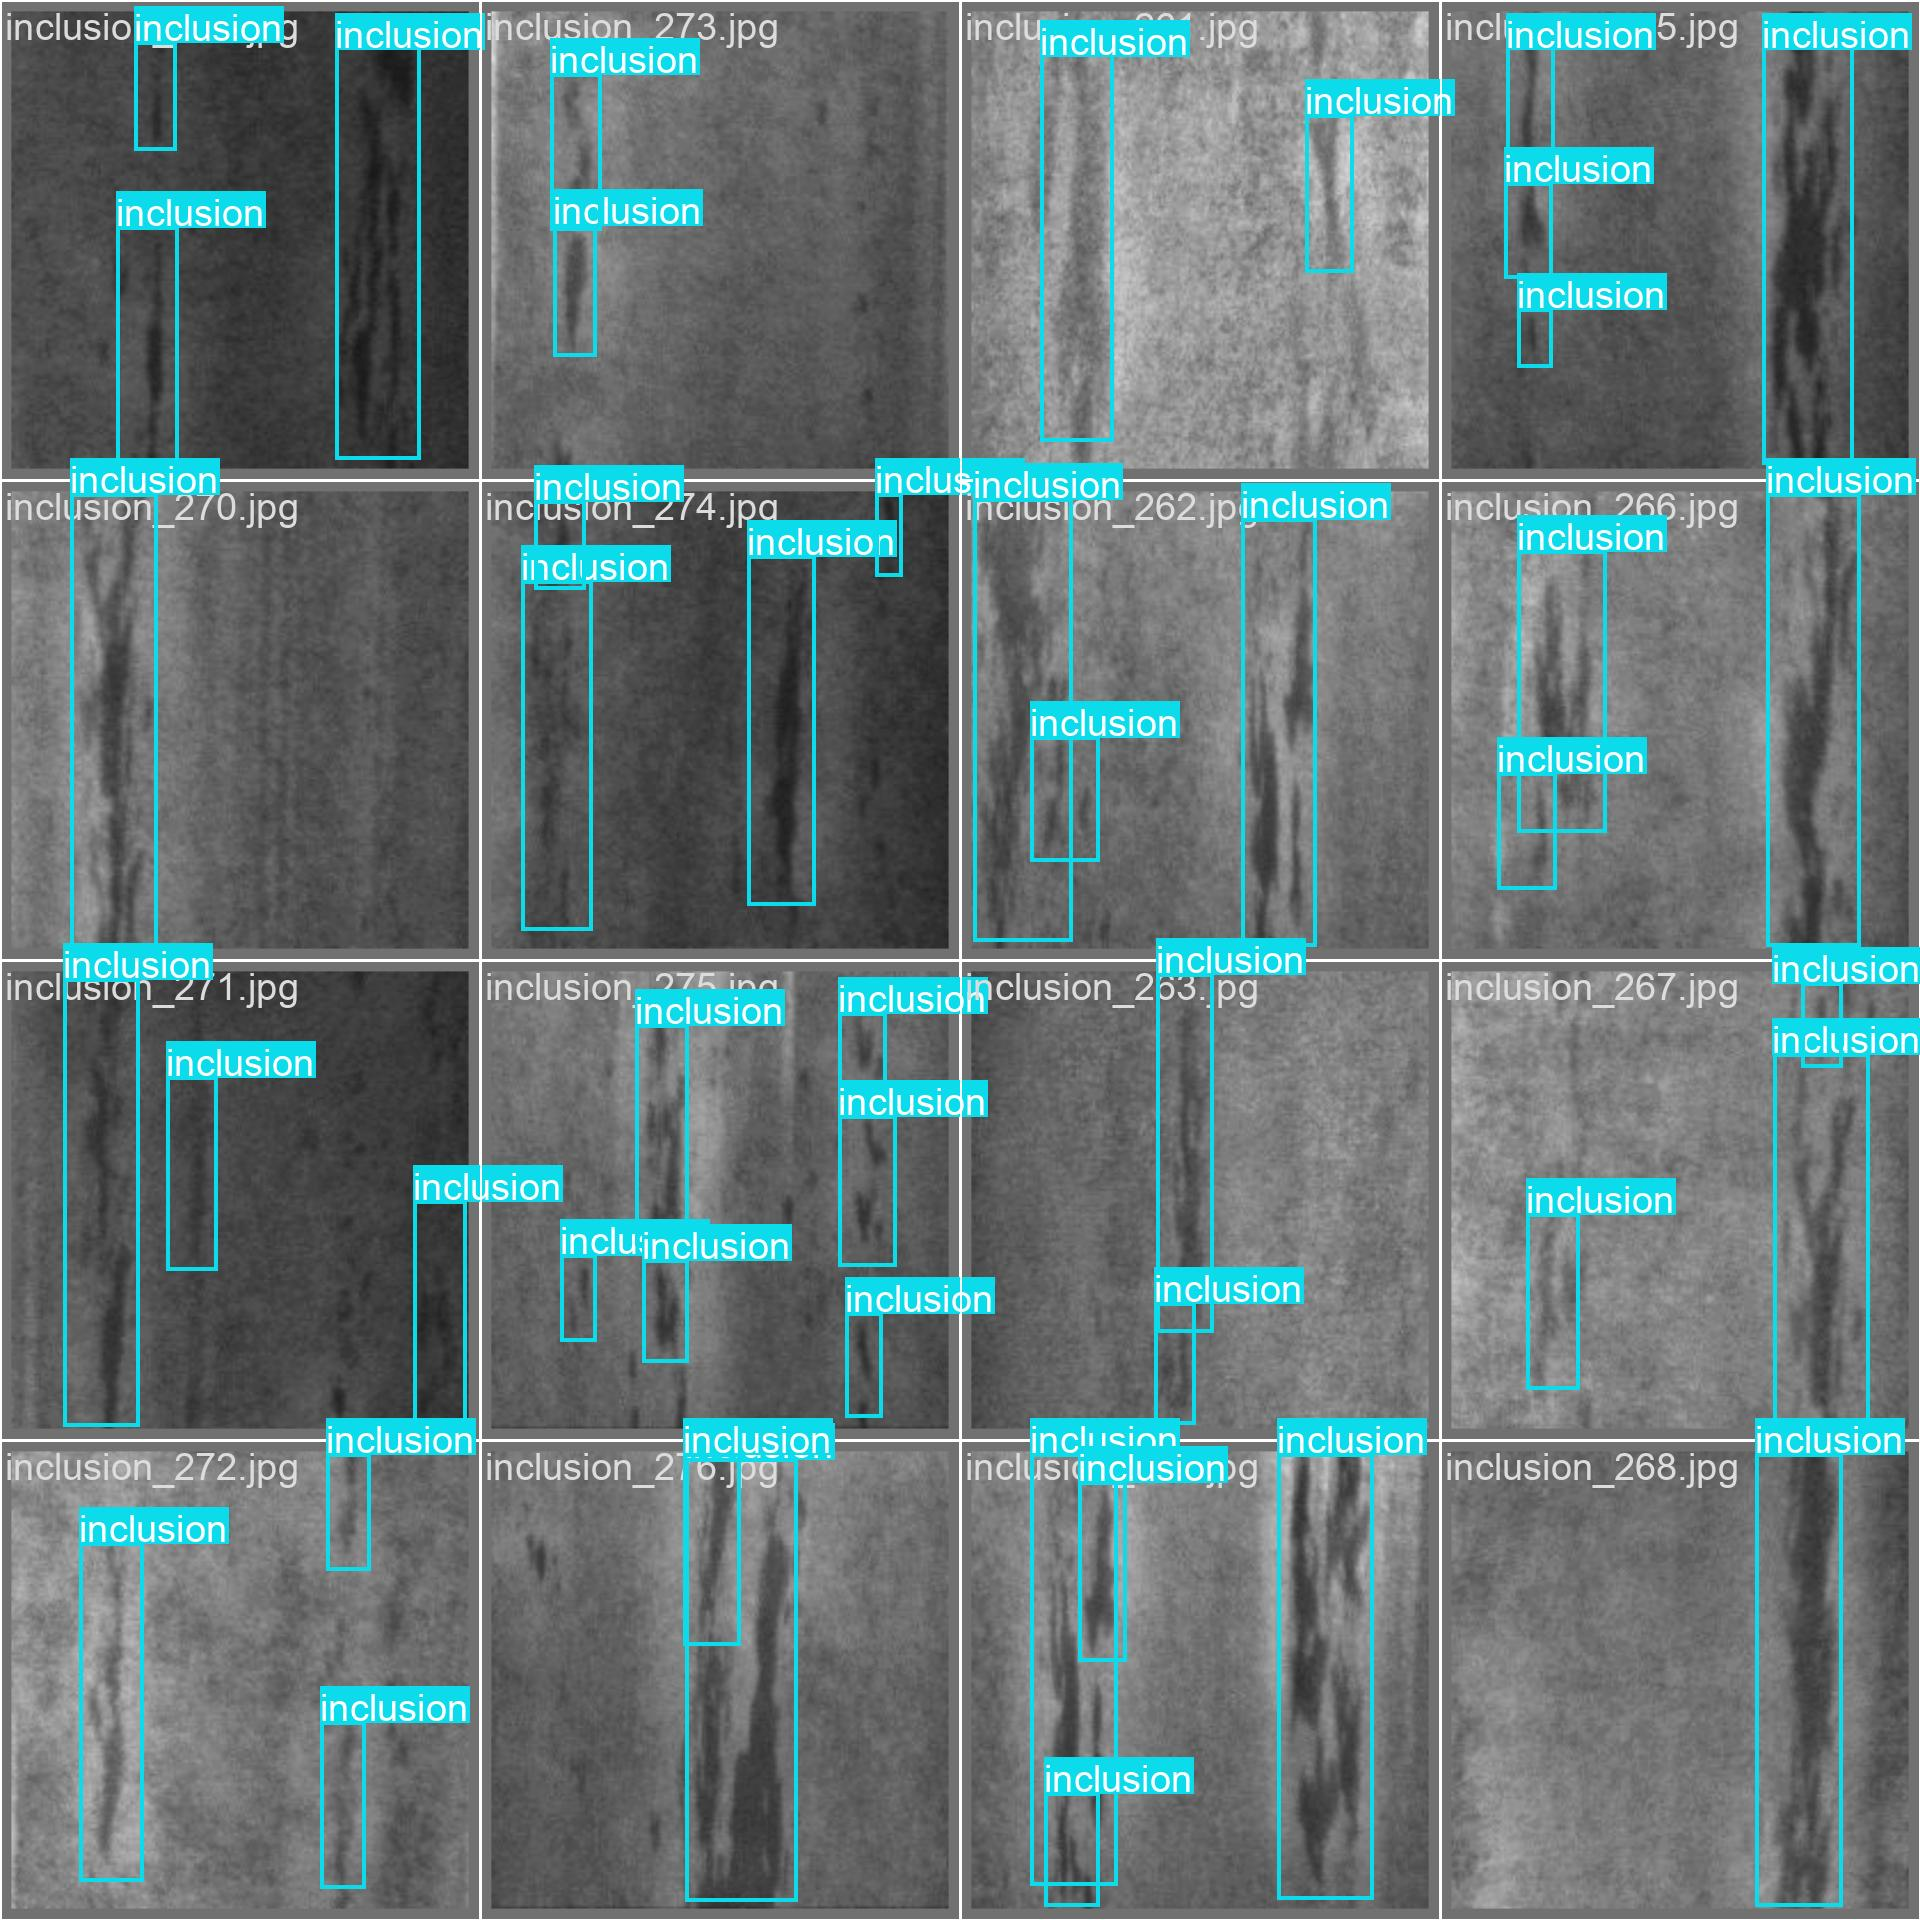
\includegraphics[width=0.2\linewidth]{img/val_batch2_labelsm.jpg}
		\caption{نمونه‌هایی از تشخیص مدل}
	\end{figure}
	
	
	%--------------------------------------------------
	
	\subsection{مقایسه با \lr{YOLOv8n} استاندارد و \lr{YOLOv8n-GSE}}
	
	مدل پایه‌ی \lr{YOLOv8n} به عنوان مبنای مقایسه (Baseline) در نظر گرفته می‌شود که به دلیل ساختار سبک، سرعت بالا و هزینه محاسباتی ناچیز، به صورت گسترده در کاربردهای بی‌درنگ استفاده می‌شود؛ با این حال، ظرفیت محدود استخراج ویژگی در معماری استاندارد آن، به ویژه در شناسایی عیوب ریز و با کنتراست پایین در تصاویر صنعتی، چالش‌زا است. نسخه اولیه توسعه‌یافته بر پایه این مدل، با نام \lr{YOLOv8n-GSE}، تنها با اضافه کردن یک بلوک \lr{GSE} به عنوان مکانیزم توجه کارآمد طراحی شد. 
	
	در مقایسه ساختاری این مدل‌ها با نسخه بزرگ‌تر \lr{YOLO11m} می‌توان به موارد زیر اشاره کرد:
	\begin{itemize}
		\item \lr{YOLOv8n} استاندارد سبک‌ترین نسخه بوده و کمترین پیچیدگی محاسباتی را دارد، اما به دلیل عدم برخورداری از مکانیزم‌های توجه و بلوک‌های استخراج ویژگی پیشرفته، پتانسیل بالایی در از دست دادن عیوب کوچک دارد.
		\item \lr{YOLOv8n-GSE} بدون افزایش محسوس در تعداد پارامترها و بار محاسباتی، به واسطه بلوک \lr{GSE} توانایی تفکیک ویژگی‌های کانالی را بهبود بخشیده و عملکرد بهتری نسبت به \lr{YOLOv8n} پایه ارائه می‌دهد.
		\item \lr{YOLO11m} دارای پارامترهای به مراتب بیشتر و ظرفیت یادگیری بالاتری است که منجر به ثبت نتایج دقیق‌تر در برخی سناریوها می‌شود، اما در عین حال نیازمند زمان آموزش طولانی‌تر و سخت‌افزار قوی‌تر جهت استنتاج است.
	\end{itemize}
	
	%--------------------------------------------------
	
	\subsection{مقایسه با \lr{YOLOv8n-Improvement}}
	
	مدل \lr{YOLOv8n-Improvement} نسخه‌ای بهینه‌سازی‌شده با تمرکز بر تعامل هم‌افزای مکانیزم‌های توجه، بهبود جریان اطلاعات و اصلاح تابع هزینه است. این مدل با ادغام بلوک‌های \lr{CSP-ABAN} جهت ارتقای نمایش ویژگی‌ها، مکانیزم توجه \lr{GAM} برای تمرکز هم‌زمان روی ابعاد کانالی و مکانی، و همچنین استفاده از هدهای پیشرفته و تابع هزینه رگرسیون جعبه مرزی \lr{PIoUv2} طراحی شده است.
	
	در مقایسه این ساختار سفارشی با مدل استاندارد \lr{YOLO11m} نقاط تمایز زیر برجسته است:
	\begin{itemize}
		\item \lr{YOLO11m} از ظرفیت شبکه و ابعاد بزرگ‌تری برخوردار است، اما فاقد مکانیزم‌های توجه اختصاصی و هدفمند مانند \lr{GAM} و ابزارهای بهبودیافته مانند \lr{CSP-ABAN} است. این امر سبب می‌شود که افزایش پارامترها در \lr{YOLO11m} لزوماً به تمرکز روی نواحی بحرانی عیوب منجر نشود.
		\item مدل‌های سفارشی (\lr{YOLOv8n-GSE} و به‌ویژه \lr{YOLOv8n-Improvement}) به دلیل طراحی متمرکز و بهینه‌سازی هدفمند معماری، به شکل موثرتری در برابر بیش‌برازش (\lr{Overfitting}) مقاومت می‌کنند. این ساختارها با هدایت فرآیند یادگیری به سمت الگوهای پایدار عیوب، تعمیم‌پذیری بالایی روی داده‌های اعتبارسنجی نشان می‌دهند.
		\item استفاده از تابع هزینه \lr{PIoUv2} در فرآیند آموزش مدل‌های سفارشی، همگرایی سریع‌تر و دقیق‌تری را در موقعیت‌یابی جعبه‌های مرزی نسبت به توابع استاندارد مورد استفاده در \lr{YOLO11m} فراهم می‌سازد.
	\end{itemize}
	
	%--------------------------------------------------
	
	\subsection{جمع‌بندی مقایسه‌ای و تحلیل کارایی}
	
	تحلیل عملکرد مدل‌های ارزیابی‌شده نشان می‌دهد که فرآیند سفارشی‌سازی توانسته است تعادل بسیار مناسبی میان نرخ انتقال اطلاعات (سرعت استنتاج) و معیارهای صحت تشخیص برقرار سازد. خلاصه‌ وضعیت هر یک از مدل‌ها به شرح زیر است:
	\begin{itemize}
		\item \lr{YOLOv8n}: بسیار سبک و سریع، اما با دقت محدودتر در بازرسی‌های حساس صنعتی.
		\item \lr{YOLOv8n-GSE} اولیه: سبک و سریع با بهبودهای ساختاری کارآمد بدون تحمیل سربار محاسباتی جدی.
		\item \lr{YOLOv8n-Improvement}: کارآمدترین نسخه از نظر مصالحه بین سرعت و دقت، مقاوم در برابر بیش‌برازش و توانمند در آشکارسازی عیوب چندگانه با نرخ تشخیص مثبت کاذب بسیار پایین.
		\item \lr{YOLO11m}: ساختار بزرگ با پارامترهای زیاد و ظرفیت یادگیری بالا که اگرچه دقت اسمی مطلوبی در برخی معیارها به دست می‌دهد، اما زمان استنتاج و بار محاسباتی سنگینی را تحمیل می‌کند.
	\end{itemize}
	
	با وجود مقیاس بزرگ‌تر مدل \lr{YOLO11m}، ارزیابی نتایج تجربی نشان می‌دهد که این افزایش ابعاد، بهبود چشمگیر و متمایزکننده‌ای را در خروجی نهایی حاصل نکرده است. در واقع، بهبودهای جزئی حاصل‌شده توسط \lr{YOLO11m} در مقایسه با افزایش توان پردازشی مورد نیاز و خطر بیش‌برازش در مجموعه‌های داده محدود، توجیه فنی و اقتصادی کافی ندارد. در مقابل، مدل‌های سفارشی‌سازی شده (\lr{YOLOv8n-GSE} و \lr{YOLOv8n-Improvement}) با حفظ سرعت استنتاج بالا در لبه شبکه و دستیابی به نتایج مناسب بر روی داده‌های اعتبارسنجی، به عنوان گزینه‌های بهینه برای پیاده‌سازی در سیستم‌های بازرسی صنعتی بلادرنگ شناخته می‌شوند.
	
	
	
	
	\section{پیاده‌سازی فازی}
	\subsection{طراحی و پیاده‌سازی سیستم کنترل فازی مبتنی بر خروجی YOLO}
	
	در این بخش، به منظور تبدیل خروجی مدل آشکارساز شیء به یک تصمیم کنترلی سطح بالا، از یک سیستم استنتاج فازی (\lr{Fuzzy Inference System}) استفاده شده است. هدف این سیستم، تبدیل اطلاعات حاصل از تشخیص عیوب سطحی به یک فرمان کنترلی پیوسته برای تنظیم سرعت خط تولید می‌باشد.
	
	%--------------------------------------------------
	
	
	\subsubsection{استخراج اطلاعات از خروجی YOLO}
	
	مدل \lr{YOLO} پس از انجام آشکارسازی، برای هر شیء شناسایی‌شده اطلاعات زیر را تولید می‌کند:
	
	\begin{itemize}
		\item مختصات جعبه مرزی (\lr{Bounding Box})
		\item شناسه کلاس
		\item میزان اطمینان (\lr{Confidence Score})
	\end{itemize}
	
	برای استفاده از این خروجی در سیستم فازی، ابتدا یک معیار ریسک وزندار تعریف شده است. برای هر کلاس، یک ضریب ریسک از پیش تعیین‌شده در نظر گرفته شده است:
	
	\[
	\text{Weighted Risk} = \sum_{i=1}^{N} 
	\left(
	\frac{Area_i}{ImageArea}
	\times RiskFactor_i
	\right)
	\times 10
	\]
	
	که در آن:
	
	\begin{itemize}
		\item $Area_i$ مساحت جعبه مرزی شیء $i$
		\item $ImageArea$ مساحت کل تصویر
		\item $RiskFactor_i$ ضریب ریسک متناظر با کلاس
	\end{itemize}
	
	این مقدار در بازه $[0,1]$ نرمال‌سازی می‌شود. همچنین میانگین اطمینان تشخیص‌ها به صورت زیر محاسبه می‌شود:
	
	\[
	\text{Mean Confidence} = \frac{1}{N} \sum_{i=1}^{N} Conf_i
	\]
	
	در صورت عدم وجود تشخیص، ریسک برابر صفر و اطمینان برابر یک در نظر گرفته شده است (به معنای نبود تهدید).
	
	بنابراین خروجی YOLO به دو ورودی عددی برای سیستم فازی تبدیل می‌شود:
	
	\begin{itemize}
		\item امتیاز ریسک نرمال‌شده
		\item میانگین میزان اطمینان مدل
	\end{itemize}
	
	%--------------------------------------------------
	
	\subsubsection{ساختار سیستم استنتاج فازی}
	
	سیستم طراحی‌شده از نوع \lr{Mamdani Fuzzy Inference System} می‌باشد و شامل:
	
	\begin{itemize}
		\item دو متغیر ورودی (\lr{Antecedent})
		\item یک متغیر خروجی (\lr{Consequent})
		\item مجموعه‌ای از قوانین فازی
	\end{itemize}
	
	\paragraph{ورودی‌ها}
	
	\begin{enumerate}
		\item \textbf{Risk Score} در بازه $[0,1]$
		\item \textbf{Confidence} در بازه $[0,1]$
	\end{enumerate}
	
	هر ورودی دارای سه مجموعه فازی می‌باشد:
	
	\[
	\{Low,\; Medium,\; High\}
	\]
	
	\paragraph{خروجی}
	
	متغیر خروجی با عنوان \lr{Speed Change} در بازه $[-1,1]$ تعریف شده است که شامل سه مجموعه فازی است:
	
	\[
	\{Brake,\; Maintain,\; Accelerate\}
	\]
	
	%--------------------------------------------------
	
	\subsubsection{انتخاب توابع عضویت گاوسی}
	
	برای تمامی متغیرها از تابع عضویت گاوسی (\lr{Gaussian Membership Function}) استفاده شده است:
	
	\[
	\mu(x) = e^{-\frac{(x-c)^2}{2\sigma^2}}
	\]
	
	که در آن $c$ مرکز تابع و $\sigma$ انحراف معیار است.
	
	\paragraph{دلایل انتخاب تابع گاوسی:}
	
	\begin{itemize}
		\item پیوستگی و مشتق‌پذیری کامل (رفتار نرم و بدون شکست ناگهانی)
		\item مناسب برای مدل‌سازی عدم قطعیت تدریجی
		\item جلوگیری از تغییرات ناگهانی در خروجی کنترل
		\item هموارسازی تصمیم‌گیری در نواحی مرزی بین \lr{Low}، \lr{Medium} و \lr{High}
	\end{itemize}
	
	در کاربرد صنعتی، تصمیم‌گیری ناگهانی می‌تواند منجر به رفتار ناپایدار سیستم شود؛ لذا استفاده از تابع گاوسی باعث انتقال نرم بین حالات مختلف می‌شود.
	
	%--------------------------------------------------
	
	
	\subsubsection{قوانین فازی طراحی‌شده}
	
	قوانین به صورت ترکیب منطقی AND بین ورودی‌ها تعریف شده‌اند. نمونه‌ای از قوانین:
	
	\begin{itemize}
		\item اگر ریسک کم و اطمینان زیاد باشد $\leftarrow$ افزایش سرعت
		\item اگر ریسک متوسط و اطمینان زیاد باشد $\leftarrow$ کاهش سرعت
		\item اگر ریسک بالا باشد $\leftarrow$ کاهش سرعت (صرف‌نظر از اطمینان)
	\end{itemize}
	
	به طور کلی:
	
	\begin{itemize}
		\item ریسک پایین $\leftarrow$ تمایل به افزایش سرعت
		\item ریسک متوسط $\leftarrow$ رفتار محافظه‌کارانه
		\item ریسک بالا $\leftarrow$ کاهش سرعت قطعی
	\end{itemize}
	
	وجود متغیر اطمینان باعث می‌شود تصمیم تنها بر اساس اندازه عیب نباشد، بلکه میزان اعتماد مدل نیز لحاظ گردد. برای مثال:
	
	\begin{itemize}
		\item ریسک کم ولی اطمینان پایین $\leftarrow$ حفظ سرعت (عدم تصمیم تهاجمی)
		\item ریسک بالا و اطمینان بالا $\leftarrow$ ترمز قوی
	\end{itemize}
	
	%--------------------------------------------------
	
	\subsubsection{فرآیند استنتاج}
	
	مراحل پردازش به صورت زیر است:
	
	\begin{enumerate}
		\item \textbf{Fuzzification}: تبدیل مقادیر عددی ریسک و اطمینان به درجات عضویت
		\item \textbf{Rule Evaluation}: اعمال قوانین با استفاده از عملگر AND (مینیمم)
		\item \textbf{Aggregation}: ترکیب خروجی قوانین
		\item \textbf{Defuzzification}: تبدیل خروجی فازی به مقدار عددی (مرکز سطح)
	\end{enumerate}
	
	خروجی نهایی عددی در بازه $[-1,1]$ است:
	
	\begin{itemize}
		\item مقدار نزدیک به $-1$ $\leftarrow$ کاهش شدید سرعت
		\item مقدار نزدیک به $0$ $\leftarrow$ حفظ سرعت
		\item مقدار نزدیک به $1$ $\leftarrow$ افزایش سرعت
	\end{itemize}
	
	حال برای هر مدل \lr{Yolov}، خروجی‌های مربوط به بخش فازی آن را نمایش می‌دهیم.
	بدیهی است که هرچه مدل \lr{Yolov} اطلاعات دقیق‌تری به مدل فازی بدهد، نتایج این مدل نیز بهتر خواهد بود.
	بنابراین انتظار داریم که نتایج مدل \lr{Yolov11m}، از دو مدل دیگر بهتر شود همچنین دو مدل دیگر نیز نتایجی تا حدی مشابه و در برخی موارد مدل \lr{Yolov8-Improvement} بهتر عمل نماید.
	\subsection{خروجی فازی مربوط به مدل \lr{YOLO8n-GSE}}
	
	% ---------- Figure 1 ----------
	\begin{figure}[!htbp]
		\centering
		\begin{subfigure}{0.45\linewidth}
			
\includegraphics[width=\linewidth]{img/crazing_283.jpg}
		\end{subfigure}
		\hfill
		\begin{subfigure}{0.45\linewidth}
			
\includegraphics[width=\linewidth]{img/crazing_297.jpg}
		\end{subfigure}
		
		\vspace{0.3cm}
		
		\begin{subfigure}{0.45\linewidth}
			
\includegraphics[width=\linewidth]{img/inclusion_259.jpg}
		\end{subfigure}
		\hfill
		\begin{subfigure}{0.45\linewidth}
			
\includegraphics[width=\linewidth]{img/inclusion_261.jpg}
		\end{subfigure}
		
		\caption{خروجی‌های فازی مدل \lr{YOLOV8n-GSE} (نمونه اول)}
	\end{figure}
	
	% ---------- Figure 2 ----------
	\begin{figure}[!htbp]
		\centering
		\begin{subfigure}{0.45\linewidth}
			
\includegraphics[width=\linewidth]{img/pitted_surface_277.jpg}
		\end{subfigure}
		\hfill
		\begin{subfigure}{0.45\linewidth}
			
\includegraphics[width=\linewidth]{img/rolled-in_scale_242.jpg}
		\end{subfigure}
		
		\vspace{0.3cm}
		
		\begin{subfigure}{0.45\linewidth}
			
\includegraphics[width=\linewidth]{img/rolled-in_scale_256.jpg}
		\end{subfigure}
		\hfill
		\begin{subfigure}{0.45\linewidth}
			
\includegraphics[width=\linewidth]{img/scratches_245.jpg}
		\end{subfigure}
		
		\caption{خروجی‌های فازی مدل \lr{YOLOV8n-GSE} (نمونه دوم)}
	\end{figure}

	\subsection{خروجی فازی مربوط به مدل \lr{YOLOV11m}}
	
	% ---------- Figure 1 ----------
	\begin{figure}[!htbp]
		\centering
		\begin{subfigure}{0.45\linewidth}
			
\includegraphics[width=\linewidth]{img/crazing_245.jpg}
		\end{subfigure}
		\hfill
		\begin{subfigure}{0.45\linewidth}
			
\includegraphics[width=\linewidth]{img/crazing_254.jpg}
		\end{subfigure}
		
		\vspace{0.3cm}
		
		\begin{subfigure}{0.45\linewidth}
			
\includegraphics[width=\linewidth]{img/inclusion_260.jpg}
		\end{subfigure}
		\hfill
		\begin{subfigure}{0.45\linewidth}
			
\includegraphics[width=\linewidth]{img/inclusion_269.jpg}
		\end{subfigure}
		
		\caption{خروجی‌های فازی مدل \lr{YOLOV11m} (نمونه اول)}
	\end{figure}
	
	% ---------- Figure 2 ----------
	\begin{figure}[!htbp]
		\centering
		\begin{subfigure}{0.45\linewidth}
			
\includegraphics[width=\linewidth]{img/patches_261.jpg}
		\end{subfigure}
		\hfill
		\begin{subfigure}{0.45\linewidth}
			
\includegraphics[width=\linewidth]{img/patches_266.jpg}
		\end{subfigure}
		
		\vspace{0.3cm}
		
		\begin{subfigure}{0.45\linewidth}
			
\includegraphics[width=\linewidth]{img/rolled-in_scale_255.jpg}
		\end{subfigure}
		\hfill
		\begin{subfigure}{0.45\linewidth}
			
\includegraphics[width=\linewidth]{img/rolled-in_scale_281.jpg}
		\end{subfigure}
		
		\caption{خروجی‌های فازی مدل \lr{YOLOV11m} (نمونه دوم)}
	\end{figure}
	
	
	\subsection{خروجی فازی مربوط به مدل \lr{YOLOV8n-Improvement}}
	
	\begin{figure}[htbp]
		\centering
		
\includegraphics[width=0.4\linewidth]{img/pitted_surface_270.jpg}
		\hfill
		
\includegraphics[width=0.4\linewidth]{img/rolled-in_scale_262.jpg}
		\hfill
		
\includegraphics[width=0.4\linewidth]{img/rolled-in_scale_270.jpg}
		\caption{خروجی‌های مربوط به فازی برای مدل \lr{YOLOV8n-Improvement}}
	\end{figure}
	
	
	\subsection{خروجی فازی مربوط به مدل \lr{YOLOV8n}}
	
	\begin{figure}[htbp]
		\centering
		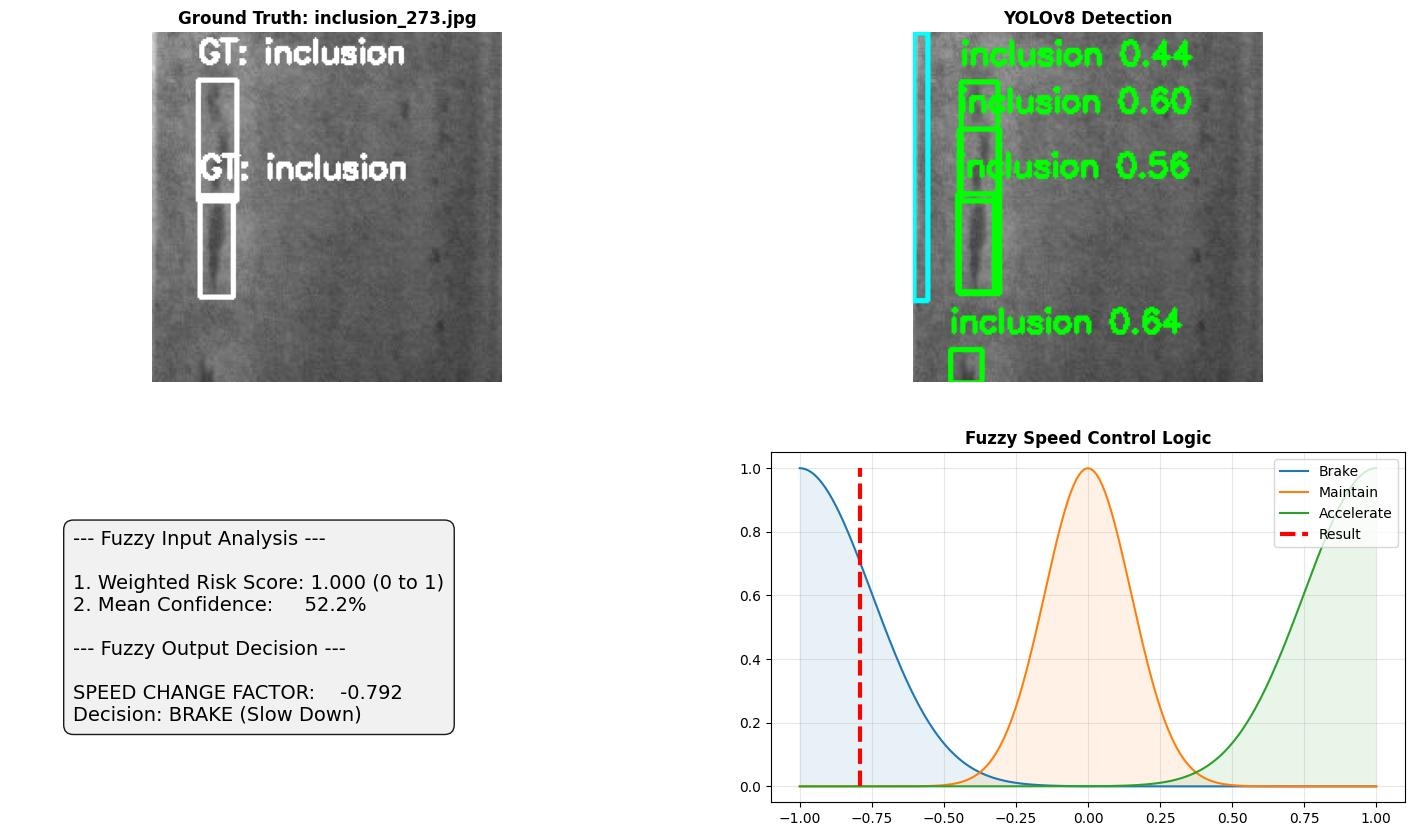
\includegraphics[width=0.4\linewidth]{img/inclusion_273n.jpg}
		\hfill
		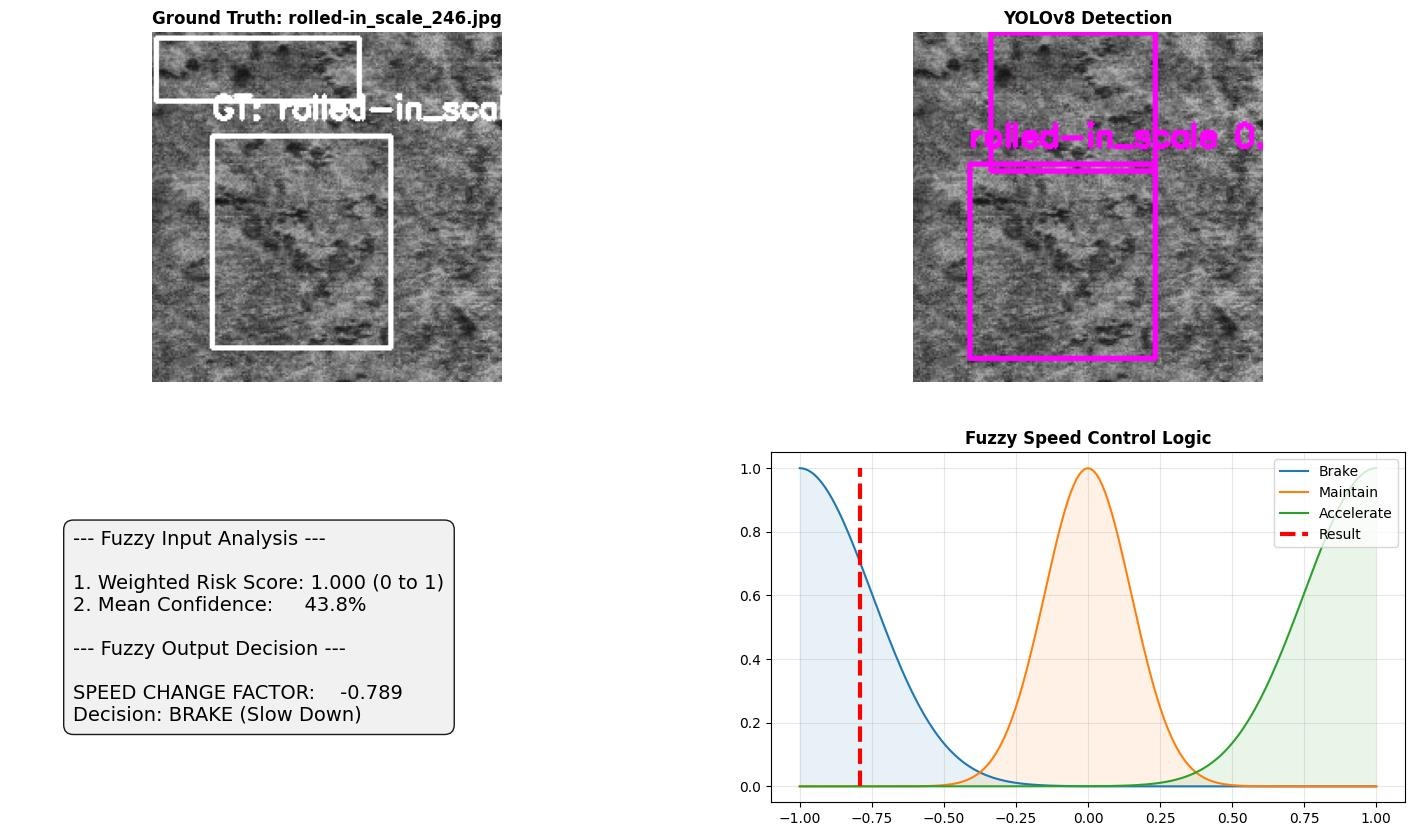
\includegraphics[width=0.4\linewidth]{img/rolled-in_scale_246n.jpg}
		\hfill
		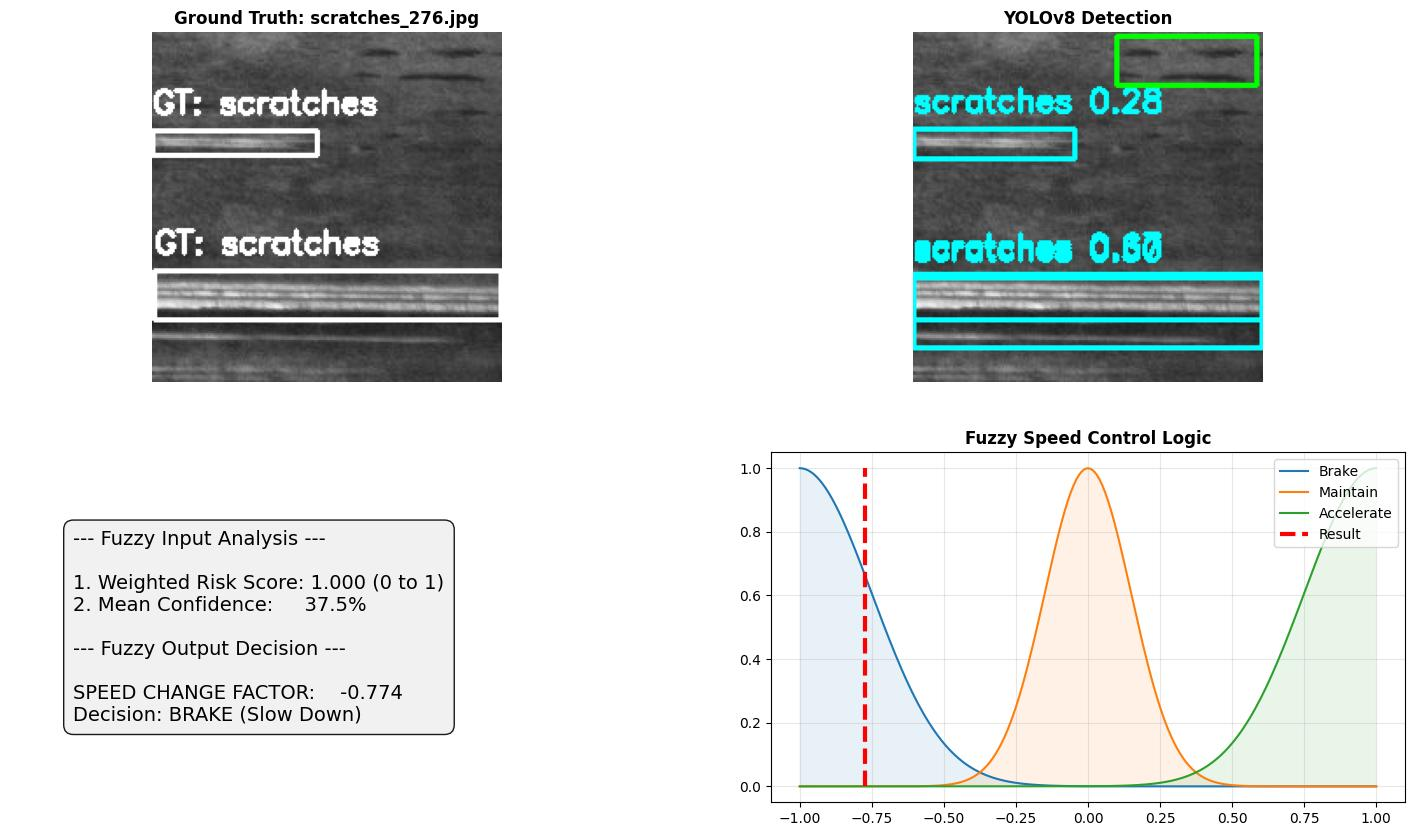
\includegraphics[width=0.4\linewidth]{img/scratches_276n.jpg}
		\caption{خروجی‌های مربوط به فازی برای مدل \lr{YOLOV8n-Improvement}}
	\end{figure}

	
	\newpage
	\section{شبیه‌سازی حلقه‌بسته کنترل هوشمند نوار نقاله}
	
	در این بخش، یک سیستم کنترل حلقه‌بسته مبتنی بر بینایی ماشین و منطق فازی طراحی و پیاده‌سازی شده است. هدف این سیستم، تنظیم دینامیکی سرعت نوار نقاله بر اساس میزان عیوب تشخیص‌داده‌شده توسط مدل \lr{YOLO} می‌باشد. ساختار کلی سیستم ترکیبی از یادگیری عمیق برای تشخیص و منطق فازی برای تصمیم‌گیری کنترلی است.
	
	%--------------------------------------------------
	
	\subsection{تولید ویدئوی شبیه‌سازی}
	
	به منظور ایجاد یک سناریوی دینامیک مشابه شرایط واقعی خط تولید، تصاویر مجموعه اعتبارسنجی به یک فایل ویدئویی تبدیل شدند. در این فرآیند:
	
	\begin{itemize}
		\item تصاویر خوانده شده و بر اساس نام مرتب شدند.
		\item تمامی تصاویر به اندازه $640 \times 640$ تغییر اندازه داده شدند.
		\item با استفاده از \lr{VideoWriter} و کدک \lr{mp4v}، ویدئو با نرخ 5 فریم بر ثانیه ساخته شد.
		\item هر تصویر چندین بار در ویدئو تکرار شد تا حرکت طبیعی‌تر شبیه‌سازی گردد.
	\end{itemize}
	
	این ویدئو به عنوان ورودی سیستم کنترل مورد استفاده قرار گرفت.
	
	%--------------------------------------------------
	
	\subsection{تعریف پارامترهای سیستم کنترل}
	
	پارامترهای اصلی کنترل به صورت زیر تعریف شدند:
	
	\begin{itemize}
		\item سرعت اولیه: $0.5$
		\item حداقل سرعت مجاز: $0.1$
		\item حداکثر سرعت مجاز: $1.0$
		\item ضریب تغییر نرم سرعت: $0.1$
	\end{itemize}
	
	سرعت به صورت نرمال‌شده در بازه $[0,1]$ مدل‌سازی شده است.
	
	%--------------------------------------------------
	
	\subsection{مدل‌سازی اثر سرعت بر کیفیت تصویر}
	
	به منظور شبیه‌سازی شرایط واقعی، افزایش سرعت منجر به تاری حرکتی تصویر می‌شود. این اثر با استفاده از یک کرنل خطی افقی پیاده‌سازی شد. اندازه کرنل متناسب با مقدار سرعت تغییر می‌کند:
	
	\[
	KernelSize \propto Speed
	\]
	
	هرچه سرعت بیشتر باشد، تاری تصویر افزایش یافته و تشخیص دشوارتر می‌شود. این بخش نقش مهمی در ایجاد فیدبک واقعی در سیستم دارد.
	
	%--------------------------------------------------
	
	\subsection{مراحل اجرای حلقه بسته}
	
	برای هر فریم از ویدئو، مراحل زیر اجرا می‌شود:
	
	\begin{enumerate}
		\item اعمال تاری حرکتی متناسب با سرعت فعلی
		\item اجرای مدل \lr{YOLO} برای تشخیص عیوب
		\item محاسبه ریسک وزندار بر اساس مساحت عیوب و ضرایب ریسک کلاس‌ها
		\item محاسبه میانگین اطمینان تشخیص
		\item ارسال ریسک و اطمینان به سیستم فازی
		\item دریافت خروجی کنترلی و به‌روزرسانی سرعت
	\end{enumerate}
	
	%--------------------------------------------------
	
	\subsection{محاسبه ریسک وزندار}
	
	ریسک کلی تصویر به صورت زیر محاسبه می‌شود:
	
	\[
	Risk = \sum_{i=1}^{N} 
	\left(
	\frac{Area_i}{ImageArea}
	\times RiskFactor_i
	\right)
	\times 10
	\]
	
	که در آن:
	
	\begin{itemize}
		\item $Area_i$ مساحت جعبه مرزی عیب
		\item $ImageArea$ مساحت کل تصویر
		\item $RiskFactor_i$ ضریب اهمیت هر کلاس
	\end{itemize}
	
	مقدار نهایی در بازه $[0,1]$ محدود می‌شود. همچنین میانگین اطمینان مدل نیز محاسبه شده و به عنوان ورودی دوم سیستم فازی استفاده می‌شود.
	
	%--------------------------------------------------
	
	\subsection{تصمیم‌گیری فازی}
	
	سیستم فازی با دریافت دو ورودی:
	
	\begin{itemize}
		\item امتیاز ریسک
		\item میانگین اطمینان
	\end{itemize}
	
	یک خروجی در بازه $[-1,1]$ تولید می‌کند:
	
	\begin{itemize}
		\item مقدار منفی: کاهش سرعت
		\item مقدار نزدیک صفر: حفظ سرعت
		\item مقدار مثبت: افزایش سرعت
	\end{itemize}
	
	سرعت جدید به صورت زیر محاسبه می‌شود:
	
	\[
	Speed_{new} = Speed_{current} + (\alpha \times Output_{fuzzy})
	\]
	
	که در آن $\alpha = 0.1$ ضریب نرم‌سازی تغییر سرعت است.
	
	در نهایت سرعت در بازه مجاز محدود می‌شود:
	
	\[
	Speed \in [0.1, 1.0]
	\]
	
	%--------------------------------------------------
	
	\subsection{نمایش اطلاعات و ذخیره نتایج}
	
	در هر فریم اطلاعات زیر روی تصویر نمایش داده می‌شود:
	
	\begin{itemize}
		\item سرعت فعلی (با رنگ‌بندی سطح خطر)
		\item مقدار ریسک
		\item نوع تصمیم کنترلی (کاهش، حفظ یا افزایش سرعت)
	\end{itemize}
	
	ویدئوی خروجی با تمامی حاشیه‌نویسی‌ها ذخیره می‌شود.
	
	%--------------------------------------------------
	
	\subsection{تحلیل عملکرد سیستم}
	
	در پایان شبیه‌سازی، نمودار تغییرات سرعت و ریسک در طول زمان رسم می‌شود. این نمودار امکان بررسی موارد زیر را فراهم می‌کند:
	
	\begin{itemize}
		\item واکنش سرعت نسبت به افزایش ریسک
		\item میزان پایداری سیستم
		\item وجود یا عدم وجود نوسانات شدید
	\end{itemize}
	
	%--------------------------------------------------
	
	\subsection{ساختار کلی حلقه فیدبک}
	
	ساختار سیستم به صورت زیر قابل نمایش است:
	
	\[
	Image
	\rightarrow YOLO
	\rightarrow Risk\ Estimation
	\rightarrow Fuzzy\ Controller
	\rightarrow Speed\ Update
	\rightarrow Motion\ Blur
	\rightarrow Image
	\]
	
	این ساختار یک حلقه کنترل بسته واقعی ایجاد می‌کند که در آن سرعت بر کیفیت تصویر اثر گذاشته و کیفیت تصویر نیز تصمیم‌گیری کنترلی را تحت تأثیر قرار می‌دهد.
	
	حال نمودار تغییرات سرعت و ریسک را در طول زمان برای هر چهار مدل ارائه می‌دهیم:
	\begin{figure}[H]
		\centering
		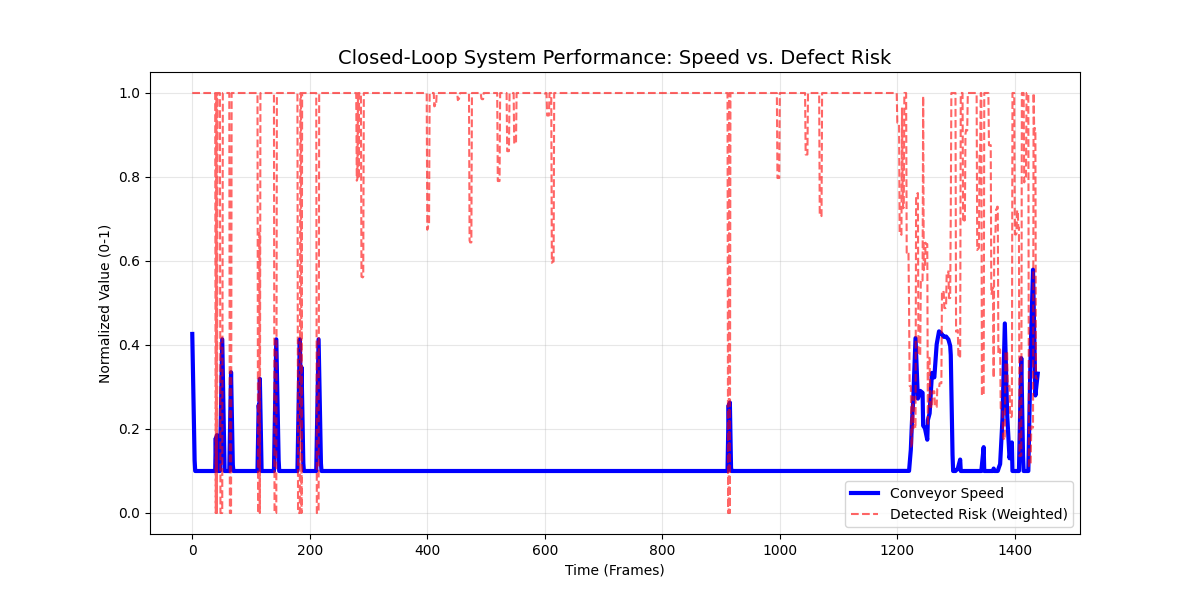
\includegraphics[width=0.9\linewidth]{img/speed_analysis8n.png}
		\caption{نمودار تغییرات سرعت و ریسک برحسب زمان(در طول فریم) برای خروجی مدل \lr{YOLO8n}}
	\end{figure}
	همانطور که مشاهده می شود، نسبت به مدل های دیگر این مدل ضعیف تر عمل کرده است و این خود بیانگر برتری مدل های سفارشی نسبت به مدل پایه است.
	\begin{figure}[H]
		\centering
		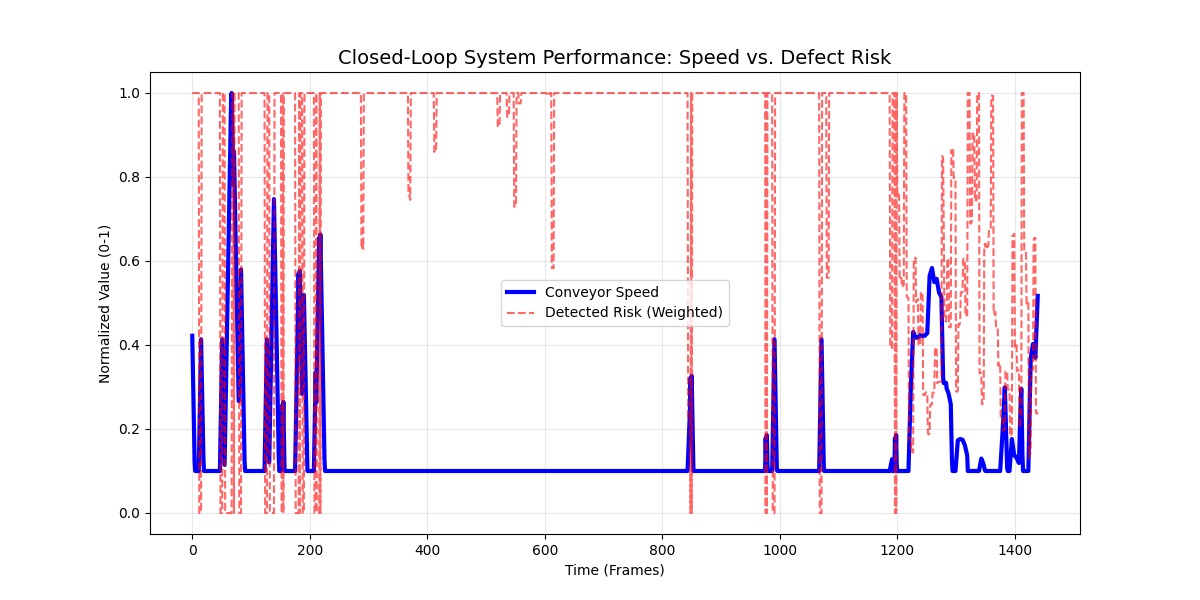
\includegraphics[width=0.9\linewidth]{img/speed_analysisg.png}
		\caption{نمودار تغییرات سرعت و ریسک برحسب زمان(در طول فریم) برای خروجی مدل \lr{YOLO8n-GSE}}
	\end{figure}
	همانطور که از نمودار مشخص است با کاهش ریسک، سرعت خط تولید بالا رفته است و با افزایش آن سرعت خط تولید پایین آمده است. در این نمودار نوسان‌های ناگهانی نیز در خط مشاهده می‌شود. این نوسان‌ها ناشی از تغییرات سرعت در طول زمان می‌باشد.
	\begin{figure}[H]
		\centering
		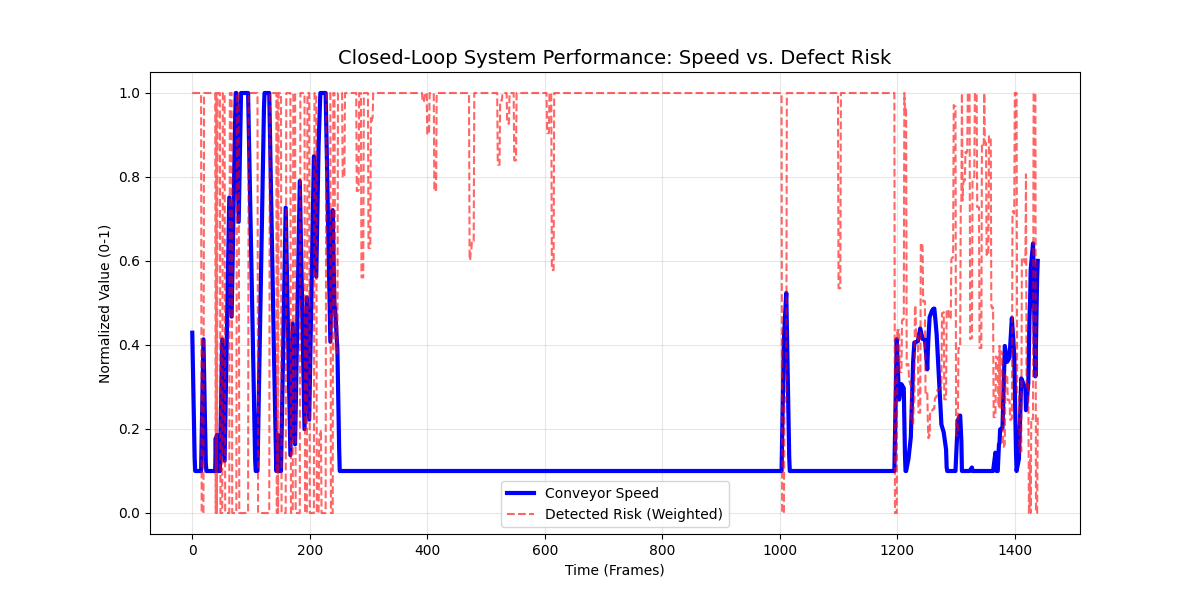
\includegraphics[width=0.9\linewidth]{img/speed_analysis_I.png}
		\caption{نمودار تغییرات سرعت و ریسک برحسب زمان(در طول فریم) برای خروجی مدل \lr{YOLO8n-Improvement}}
	\end{figure}
	در این نمودار نیز همان موارد گفته شده در بالا دیده می‌شود. خیلی نمودار تغییری نکرده است اما مقداری نوسان‌های ناگهانی کمتر شده است و مقداری از تیزی نمودار کاسته شده است اما باز هم نمی‌توان گفت که تصمیمات در تغییر سرعت به صورت پیوسته هستند.
	\begin{figure}[H]
		\centering
		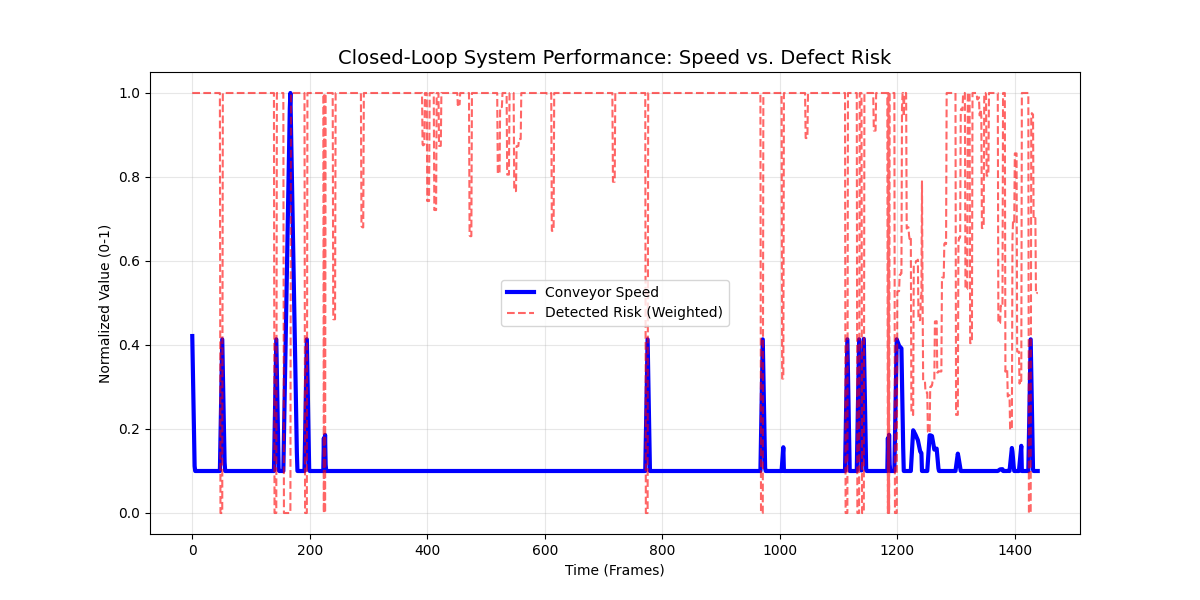
\includegraphics[width=0.9\linewidth]{img/speed_analysism.png}
		\caption{نمودار تغییرات سرعت و ریسک برحسب زمان(در طول فریم) برای خروجی مدل \lr{YOLOv11m}}
	\end{figure}
	در بین این نمودارها بهترین نتیجه برای مدل \lr{YOLOv8n-Improvement} می باشد. همانطور که در این نمودارها مشخص است خروجی بخش تشخیص تاثیر بسیار زیادی در خروجی بخش فازی دارد. بطوریکه همانطور که پیش تر هم گفته بودیم مدل سفارشی عملکرد بهتری در کنترل سرعت داشته است.
	در این نمودار نیز باز رفتار مشابه دیده می‌شود و در برخی زمان‌ها به صورت ناگهانی تصمیم به تغییر سرعت داریم. این موضوع باعث می‌شود تا خط ناپایدار شود. این رفتار به رفتار مدل فازی برمی‌گردد. چرا که هرچند ما با یک تابع گاوسی سعی کردیم تا رفتار مدل را پیوسته‌تر کنیم اما باز هم این پیوستگی خودش را در طول زمان نشان نمی‌دهد و رفتار مدل فازی به صورت صفر و یکی و نوسانی می‌شود برای اینکه رفتار آن را بهتر کنیم و سرعتی پیوسته‌تر در طول خط داشته باشیم و همچنین از تجربیات محیط هم برای سرعت خط تولید استفاده نماییم، سراغ بخش بعدی این پروژه می‌رویم و یک مدل یادگیری تقویتی آموزش می‌دهیم.
	\section{آموزش مدل \lr{RL}}
	\subsection{هدف طراحی عامل یادگیری تقویتی}
	
	هدف از به‌کارگیری \lr{Reinforcement Learning} در این پروژه، ایجاد یک مکانیزم تصمیم‌گیری تطبیقی برای تنظیم سرعت خط تولید است؛ به‌گونه‌ای که بین دو هدف متضاد زیر تعادل برقرار شود:
	
	\begin{itemize}
		\item بیشینه‌سازی بهره‌وری تولید (افزایش سرعت)
		\item کمینه‌سازی عبور عیوب پرریسک (کاهش سرعت در شرایط خطر)
	\end{itemize}
	
	در این چارچوب، عامل یادگیرنده به‌صورت تعاملی با محیط (ویدیو شبیه‌سازی‌شده خط تولید) تعامل کرده و با دریافت پاداش، سیاست بهینه را می‌آموزد.
	
	\vspace{1em}
	
	\subsection{الگوریتم مورد استفاده: \lr{Q-Learning}}
	
	روش یادگیری مورد استفاده، الگوریتم \lr{Q-Learning} مبتنی بر جدول مقدار (\lr{Q-Table}) است.
	
	رابطه به‌روزرسانی به‌صورت زیر تعریف می‌شود:
	
	\[
	Q(s,a) \leftarrow (1-\alpha)Q(s,a) + \alpha \left( r + \gamma \max_{a'} Q(s',a') \right)
	\]
	
	که در آن:
	
	\begin{itemize}
		\item $s$ : حالت فعلی
		\item $a$ : عمل انتخاب‌شده
		\item $r$ : پاداش دریافتی
		\item $s'$ : حالت بعدی
		\item $\alpha$ : نرخ یادگیری (\lr{Learning Rate})
		\item $\gamma$ : ضریب تنزیل (\lr{Discount Factor})
	\end{itemize}
	
	در پیاده‌سازی انجام‌شده:
	
	\[
	\alpha = 0.1 \qquad \gamma = 0.9
	\]
	
	\vspace{1em}
	
	\subsection{تعریف فضای حالت (\lr{State Space})}
	
	حالت سیستم ترکیبی از دو مؤلفه گسسته است:
	
	\begin{enumerate}
		\item وضعیت پیشنهاد سیستم فازی
		\item سطح سرعت فعلی نوار نقاله
	\end{enumerate}
	
	هر یک به سه سطح گسسته تقسیم شده‌اند:
	
	\[
	\text{Fuzzy State} \in \{Brake, Hold, Accelerate\}
	\]
	
	\[
	\text{Speed State} \in \{Low, Medium, High\}
	\]
	
	در نتیجه فضای حالت برابر است با:
	
	\[
	3 \times 3 = 9 \text{ حالت}
	\]
	
	که به‌صورت یک جدول سه‌بعدی با ابعاد $(3,3,3)$ مدل شده است.
	
	\vspace{1em}
	
	\subsection{فضای عمل (\lr{Action Space})}
	
	عامل می‌تواند یکی از سه عمل زیر را انتخاب کند:
	
	\begin{itemize}
		\item کاهش سرعت: $\Delta v = -0.1$
		\item حفظ سرعت: $\Delta v = 0$
		\item افزایش سرعت: $\Delta v = +0.1$
	\end{itemize}
	
	بنابراین:
	
	\[
	|A| = 3
	\]
	
	سرعت در بازه زیر محدود شده است:
	
	\[
	0.1 \leq v \leq 1.0
	\]
	
	\vspace{1em}
	
	\subsection{استراتژی اکتشاف و بهره‌برداری (\lr{Exploration-Exploitation})}
	
	برای جلوگیری از گیر افتادن در بهینه محلی، از سیاست \lr{$\epsilon$-greedy} استفاده شده است:
	
	\[
	a =
	\begin{cases}
		\text{random action} & \text{with probability } \epsilon \\
		\arg\max Q(s,a) & \text{otherwise}
	\end{cases}
	\]
	
	پارامتر $\epsilon$ به‌صورت کاهشی تنظیم شده است:
	
	\[
	\epsilon_{new} = \max(0.05, \epsilon \times 0.93)
	\]
	
	این مکانیزم باعث می‌شود سیستم در مراحل اولیه بیشتر اکتشاف انجام دهد و در مراحل پایانی به سمت بهره‌برداری حرکت کند.
	
	\vspace{1em}
	
	
	\subsection{طراحی تابع پاداش (\lr{Reward Function})}
	
	تابع پاداش به‌صورت تهاجمی طراحی شده است تا رفتار صنعتی واقع‌گرایانه ایجاد کند.
	
	\subsubsection*{مولفه‌های پاداش}
	
	\begin{enumerate}
		\item پاداش بهره‌وری:
		\[
		R_{speed} = 100 \times Speed
		\]
		
		\item جریمه ریسک بالا:
		\[
		R_{risk} = -300 \times (Risk \times Speed)
		\quad \text{if } Risk > 0.4
		\]
		
		\item هم‌راستایی با پیشنهاد فازی:
		\[
		R_{fuzzy} =
		\begin{cases}
			+50 & \text{if aligned} \\
			-50 & \text{otherwise}
		\end{cases}
		\]
	\end{enumerate}
	
	فرم کلی:
	
	\[
	R = R_{speed} + R_{risk} + R_{fuzzy}
	\]
	
	\vspace{1em}
	
	\subsection{فلسفه طراحی تابع پاداش}
	
	این تابع سه رفتار را تشویق می‌کند:
	
	\begin{itemize}
		\item حرکت به سمت سرعت بالا در شرایط ایمن
		\item کاهش سرعت هنگام افزایش ریسک
		\item هم‌گرایی تدریجی رفتار RL با منطق انسانی (خروجی فازی)
	\end{itemize}
	
	در واقع، سیستم فازی نقش نوعی \lr{Prior Knowledge} را ایفا می‌کند و عامل RL به مرور زمان می‌آموزد چه زمانی از آن تبعیت کند یا در صورت نیاز از آن فاصله بگیرد.
	
	\vspace{1em}
	
	\section{تحلیل رفتار و اثرگذاری عامل یادگیری تقویتی}
	
	\subsection{۱. پایداری یادگیری}
	
	به دلیل کوچک بودن فضای حالت (۹ حالت) و فضای عمل (۳ عمل)، الگوریتم \lr{Q-Learning} همگرایی سریعی دارد.  
	کاهش تدریجی $\epsilon$ باعث تثبیت سیاست نهایی شده و از نوسانات شدید جلوگیری می‌کند.
	
	\vspace{1em}
	
	\subsection{۲. تحلیل تعادل سرعت و ریسک}
	
	با توجه به ساختار پاداش:
	
	\begin{itemize}
		\item در ریسک پایین → جمله $R_{speed}$ غالب است → سیستم تمایل به افزایش سرعت دارد.
		\item در ریسک بالا → جمله $R_{risk}$ غالب می‌شود → کاهش سرعت بهینه می‌شود.
	\end{itemize}
	
	بنابراین سیاست نهایی یک سیاست \textbf{وابسته به شرایط محیطی} است و رفتار ثابت ندارد.
	
	\vspace{1em}
	
	\subsection{۳. نقش هم‌راستایی با فازی}
	
	مولفه $R_{fuzzy}$ باعث می‌شود RL:
	
	\begin{itemize}
		\item در مراحل اولیه سریع‌تر همگرا شود.
		\item از رفتارهای بسیار پرریسک جلوگیری کند.
	\end{itemize}
	
	در عمل، سیستم یک ساختار \lr{Hybrid Intelligent Control} ایجاد می‌کند که در آن:
	
	\begin{itemize}
		\item \lr{Fuzzy Logic} نقش راهنمای اولیه را دارد.
		\item \lr{Reinforcement Learning} سیاست بهینه بلندمدت را استخراج می‌کند.
	\end{itemize}
	
	\vspace{1em}
	
	\subsection{۴. گذار از سیستم واکنشی به سیستم پیش‌بین}
	
	در سیستم‌های سنتی، کاهش سرعت تنها پس از مشاهده خطا انجام می‌شود.  
	اما در این معماری، عامل با یادگیری از توالی حالت‌ها، رفتار آینده‌نگرانه اتخاذ می‌کند و پیش از بحرانی شدن وضعیت، سرعت را تنظیم می‌کند.
	
	حال خروجی‌های نهایی نمودار سرعت و مقدار ریسک برحسب زمان(فریم) ارائه می‌شوند. همانطور که در شکل‌های زیر مشخص می‌باشد، سرعت نوار نقاله پیوسته‌تر تغییر می‌کند و از آن حالت نوسانی دورتر شده است چرا که یادگیری تقویتی باعث می‌شود که تصمیمات فازی در طول زمان پیوسته‌تر و نه فقط صفر و یکی شود. عملا ما به جای دیدن پالس ضربه، یک تغییراتی را در بازۀ زمانی مشاهده نماییم. البته باید گفت که به صورت کامل این موضوع در این بخش حل نشده است. یعنی بهبود تا حدی حاصل شد اما باز هم تلاش کنترلی به شکل مناسبی نیست. در ادامه به سمت آموزش مدل \lr{ppo} رفتیم تا جلوی تلاش های کنترلی ناگهانی را بگیریم و به پاسخی نرم دست پیدا نماییم.
	
	\begin{figure}[H]
		\centering
		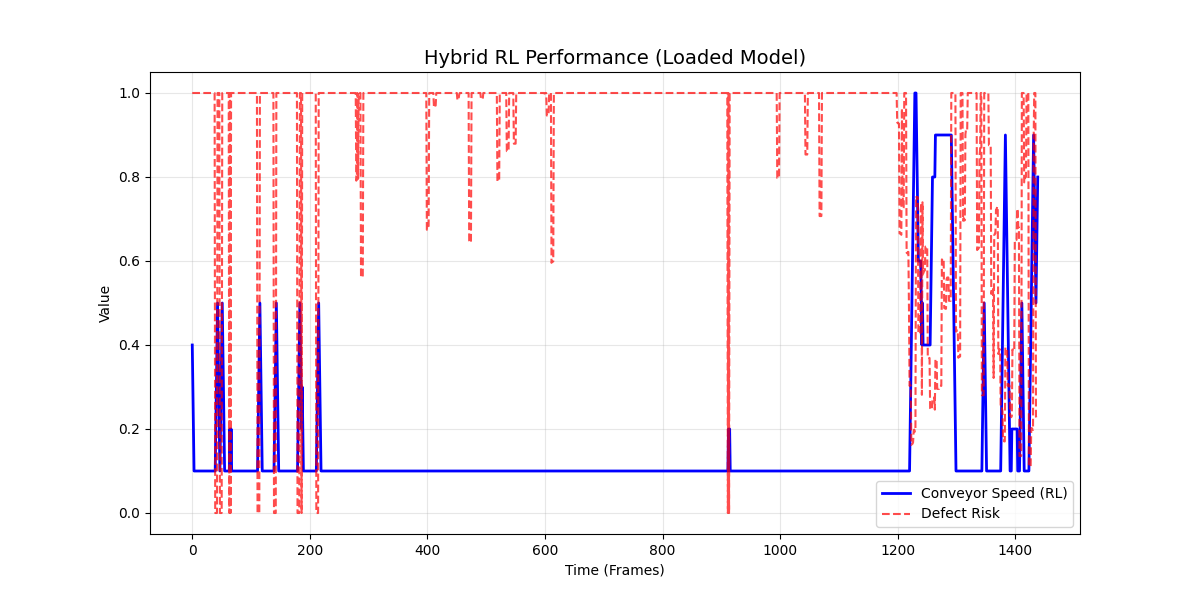
\includegraphics[width=0.8\linewidth]{img/hybrid_rl_performance8n.png}
		\caption{عملکرد مدل هیبریدی یادگیری تقویتی و فازی در طول زمان(فریم) برای خروجی \lr{Yolov8n}}
	\end{figure}
	\begin{figure}[H]
		\centering
		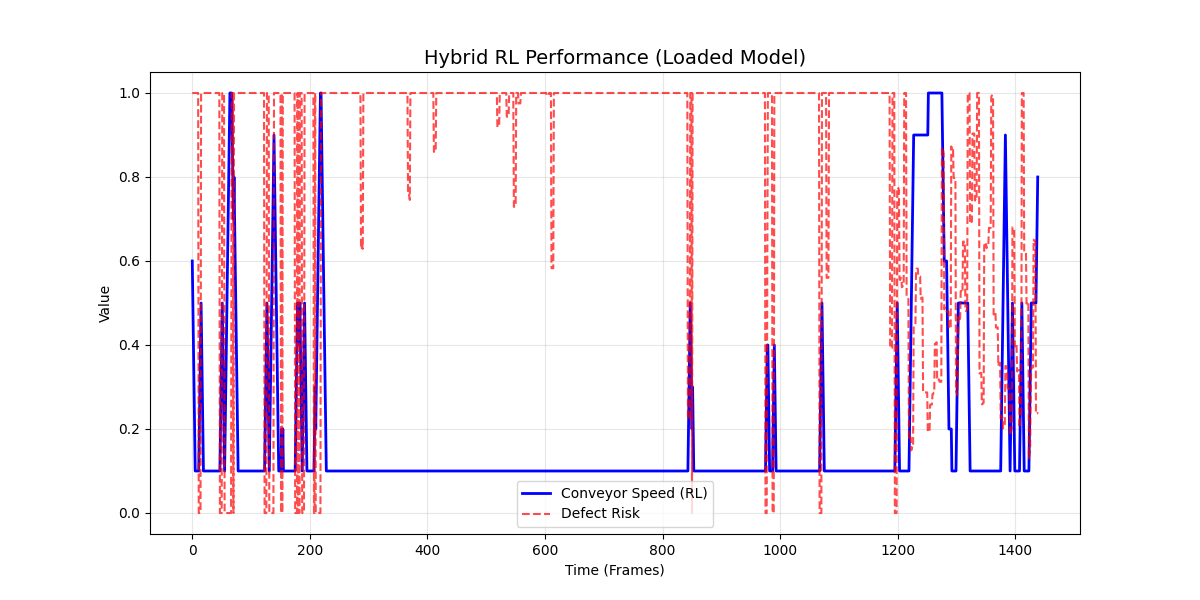
\includegraphics[width=0.8\linewidth]{img/hybrid_rl_performanceg.png}
		\caption{عملکرد مدل هیبریدی یادگیری تقویتی و فازی در طول زمان(فریم) برای خروجی \lr{Yolov8n-GSE}}
	\end{figure}
	\begin{figure}[H]
		\centering
		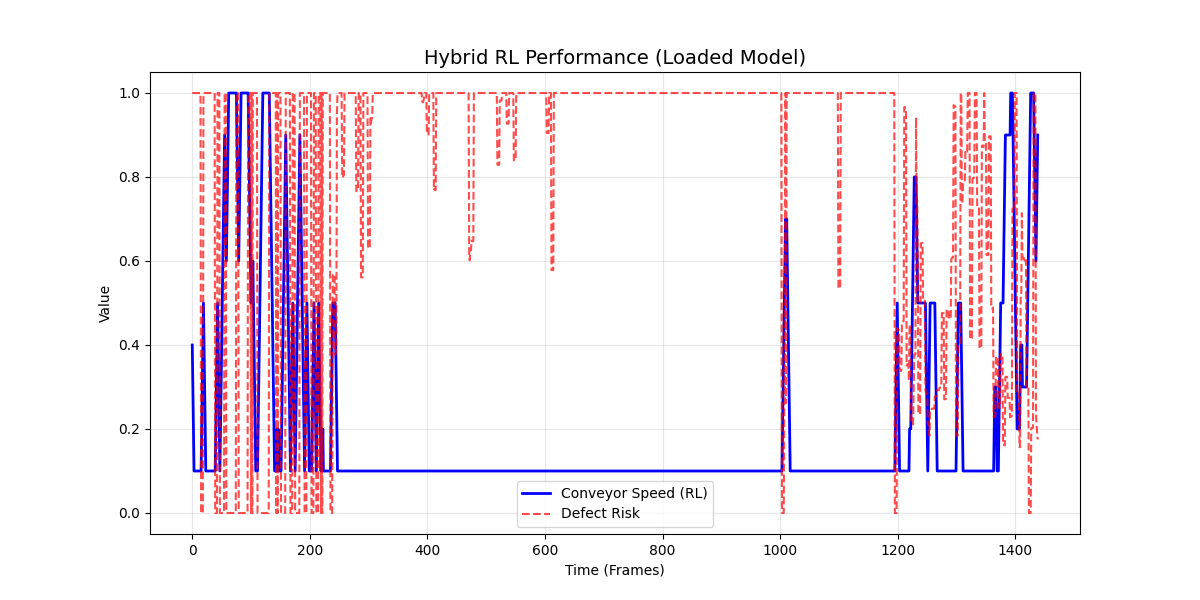
\includegraphics[width=0.8\linewidth]{img/hybrid_rl_performancei.png}
		\caption{عملکرد مدل هیبریدی یادگیری تقویتی و فازی در طول زمان(فریم) برای خروجی \lr{Yolov8n-Improvement}}
	\end{figure}
	\begin{figure}[H]
		\centering
		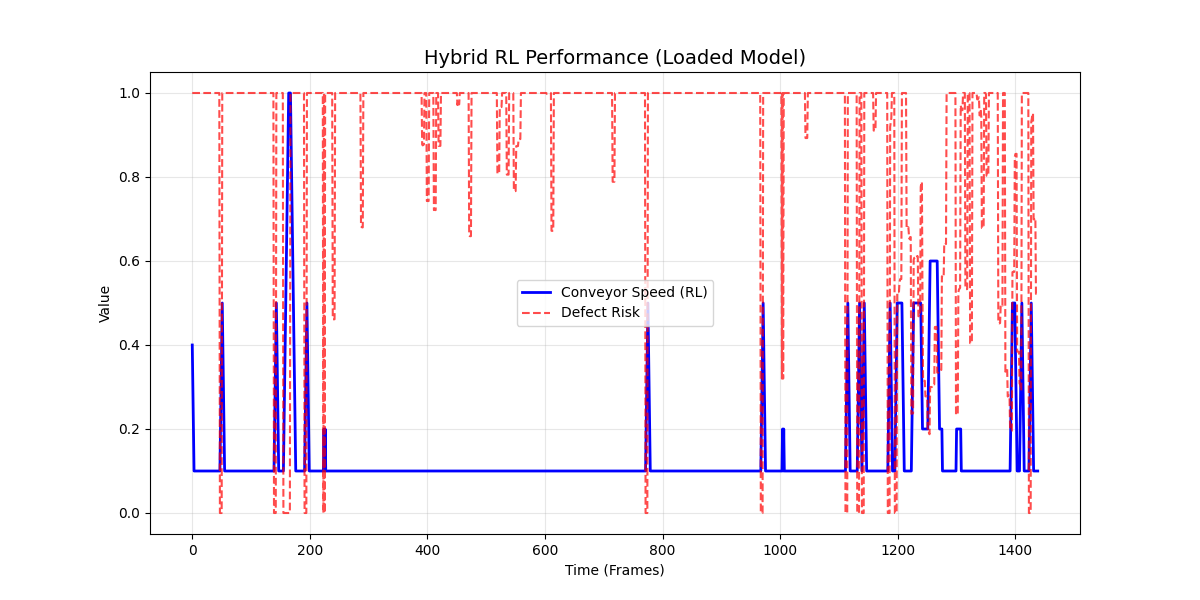
\includegraphics[width=0.8\linewidth]{img/hybrid_rl_performancem.png}
		\caption{عملکرد مدل هیبریدی یادگیری تقویتی و فازی در طول زمان(فریم) برای خروجی \lr{Yolov11m}}
	\end{figure}
	همانطور که مشاهده می‌شود، در نمودارهای دوم و سوم تغییرات سرعت پیوسته‌تر است که دلیل آن هم به خاطر خروجی‌های مناسب‌تری است که مدل‌های \lr{Yolov8n-Improvemen} و \lr{Yolov11m} فراهم می‌نمایند.
	
	البته باید گفت که در این بخش نیز به پاسخ کنترلی مناسب و دلخواه دست نیافتیم و همانطور که قابل مشاهده است، تلاش های کنترلی با فرکانس های بالا و به صورت ناگهانی اعمال می شود. در ادامه با الگوریتم \lr{ppo} این موضوع را بهبود می دهیم.
	
	\section{ppo}
	
	\subsubsection*{کنترل تطبیقی سرعت نوار نقاله با الگوریتم \lr{PPO}}
	
	به‌منظور تنظیم هوشمند سرعت نوار نقاله متناسب با وضعیت عیوب سطح، از الگوریتم یادگیری تقویتی \lr{Proximal Policy Optimization (PPO)} استفاده شد. هدف اصلی عامل کنترلی، انتخاب سرعتی مناسب برای نوار نقاله با توجه به میزان ریسک عیب‌های آشکارسازی‌شده، سطح اطمینان تشخیص مدل بینایی و شرایط عملیاتی جاری است. بدین ترتیب، در شرایطی که احتمال وجود عیب مهم یا ریسک بالا باشد، عامل باید به سمت کاهش سرعت حرکت کند و در شرایط کم‌ریسک، امکان افزایش سرعت برای حفظ بهره‌وری سیستم فراهم شود.
	
	این پیاده‌سازی برای چهار مدل آشکارسازی شامل \lr{YOLOv8n}، \lr{YOLOv8n-GSE}، \lr{YOLOv8n-Improvement} و \lr{YOLO11m} انجام شد. در تمام آزمایش‌ها، ساختار محیط، فضای حالت، فضای عمل، تابع پاداش و ابرپارامترهای آموزش \lr{PPO} ثابت نگه داشته شدند تا تفاوت نهایی عملکرد کنترل‌کننده عمدتاً ناشی از کیفیت ویژگی‌های استخراج‌شده توسط مدل آشکارسازی باشد.
	
	\paragraph{استخراج ویژگی از خروجی مدل آشکارسازی}
	
	در هر فریم، مدل \lr{YOLO} عیوب موجود در تصویر را آشکارسازی می‌کند. از خروجی آشکارساز، مجموعه‌ای از ویژگی‌های مؤثر برای تصمیم‌گیری عامل استخراج می‌شود که شامل موارد زیر است:
	
	\begin{itemize}
		\item بیشینه امتیاز ریسک عیب‌های آشکارشده؛
		\item میانگین اطمینان پیش‌بینی‌های مدل آشکارسازی؛
		\item تعداد عیوب تشخیص‌داده‌شده، نرمال‌شده نسبت به حداکثر تعداد تشخیص قابل قبول؛
		\item فاصله نزدیک‌ترین عیب از مرکز تصویر؛
		\item سرعت فعلی نوار نقاله؛
		\item خروجی کنترل‌کننده فازی مبتنی بر ریسک و اطمینان تشخیص.
	\end{itemize}
	
	امتیاز ریسک هر عیب با استفاده از مساحت نسبی جعبه مرزی و ضریب ریسک متناظر با کلاس عیب محاسبه می‌شود. به‌طور کلی، عیب‌های بزرگ‌تر یا عیب‌هایی با ضریب خطر بالاتر، امتیاز ریسک بیشتری ایجاد می‌کنند. در نتیجه، عامل \lr{PPO} تنها به وجود یا عدم وجود عیب وابسته نیست، بلکه شدت نسبی، میزان اطمینان مدل و موقعیت عیب در فریم را نیز در تصمیم‌گیری لحاظ می‌کند.
	
	\paragraph{فضای حالت و فضای عمل}
	
	بردار حالت ورودی عامل در هر گام به‌صورت زیر تعریف می‌شود:
	
	\begin{latin}
		\begin{equation}
			s_t =
			\left[
			r_t,\;
			\bar{c}_t,\;
			v_t,\;
			n_t,\;
			d_t,\;
			u^{\mathrm{fuzzy}}_t
			\right],
		\end{equation}
	\end{latin}
	
	که در آن $r_t$ بیشینه ریسک، $\bar{c}_t$ میانگین اطمینان، $v_t$ سرعت فعلی نوار نقاله، $n_t$ تعداد نرمال‌شده عیوب، $d_t$ فاصله نرمال‌شده نزدیک‌ترین عیب از مرکز تصویر و $u^{\mathrm{fuzzy}}_t$ خروجی کنترل‌کننده فازی است.
	
	فضای عمل به‌صورت گسسته و شامل سه تصمیم کنترلی تعریف شد:
	
	\begin{itemize}
		\item کاهش سرعت؛
		\item حفظ سرعت فعلی؛
		\item افزایش سرعت.
	\end{itemize}
	
	با این حال، عمل عامل به تغییر مستقیم و بزرگ در سرعت تبدیل نمی‌شود. هر عمل تنها یک گام کوچک سرعتی اعمال می‌کند. در این پروژه، مقدار گام تغییر سرعت برابر با $0.1$ در نظر گرفته شد. بنابراین، سرعت جدید نوار نقاله از رابطه زیر به‌دست می‌آید:
	
	\begin{latin}
		\begin{equation}
			v_{t+1} =
			\mathrm{clip}
			\left(
			v_t + \Delta v_t,\;
			v_{\min},\;
			v_{\max}
			\right),
			\qquad
			\Delta v_t \in \{-0.1,\;0,\;+0.1\}.
		\end{equation}
	\end{latin}
	
	این محدودسازی تضمین می‌کند که سرعت نوار نقاله همواره در بازه مجاز عملیاتی باقی بماند.
	
	\subsubsection*{طراحی تابع پاداش}
	
	تابع پاداش به‌گونه‌ای طراحی شد که عامل میان بهره‌وری خط تولید، ایمنی فرآیند بازرسی و نرمی تغییرات سرعت تعادل برقرار کند. اجزای اصلی تابع پاداش شامل هم‌راستایی با تصمیم کنترل‌کننده فازی، توجه به سطح ریسک، استفاده از اطمینان مدل آشکارسازی، پاداش سرعت مناسب در وضعیت کم‌ریسک و جریمه تغییرات ناگهانی سرعت است.
	
	به‌صورت مفهومی، تابع پاداش را می‌توان به شکل زیر نمایش داد:
	
	\begin{latin}
		\begin{equation}
			R_t =
			R_{\mathrm{fuzzy}}
			+
			R_{\mathrm{risk}}
			+
			R_{\mathrm{conf}}
			+
			R_{\mathrm{speed-risk}}
			-
			R_{\mathrm{smooth}}.
		\end{equation}
	\end{latin}
	
	در این ساختار، در صورت بالا بودن ریسک، کاهش سرعت پاداش بیشتری دریافت می‌کند و افزایش سرعت جریمه می‌شود. برعکس، هنگامی که ریسک پایین است، افزایش کنترل‌شده سرعت برای حفظ بهره‌وری خط تولید تشویق می‌شود. همچنین، میانگین اطمینان بالاتر مدل تشخیص، باعث افزایش قابلیت اتکای تصمیم عامل شده و در تابع پاداش اثر مثبت دارد.
	
	یکی از اجزای مهم تابع پاداش، جریمه تغییر ناگهانی سرعت است که به‌صورت زیر بیان می‌شود:
	
	\begin{latin}
		\begin{equation}
			R_{\mathrm{smooth}} =
			\lambda_{\Delta v}
			\left|v_{t+1}-v_t\right|.
		\end{equation}
	\end{latin}
	
	وجود این جمله باعث می‌شود عامل از تغییرات شدید، ناپایدار و غیرضروری سرعت اجتناب کند. در نتیجه، سیاست آموخته‌شده فقط به دنبال بیشینه‌سازی پاداش لحظه‌ای نیست، بلکه رفتار کنترلی پایدارتر و مناسب‌تری برای سامانه فیزیکی ارائه می‌دهد.
	
	\subsubsection*{ساختار عامل و روند آموزش}
	
	عامل \lr{PPO} با سیاست \lr{MlpPolicy} پیاده‌سازی شد. این سیاست از یک شبکه عصبی چندلایه برای تقریب سیاست تصمیم‌گیری و تابع ارزش استفاده می‌کند. بخش سیاست شامل دو لایه پنهان با $64$ نورون و بخش تابع ارزش شامل دو لایه پنهان با $128$ نورون است. استفاده از شبکه‌های مجزا برای سیاست و تابع ارزش، امکان یادگیری مناسب‌تر تصمیم کنترلی و تخمین بازده حالت را فراهم می‌کند.
	
	آموزش عامل با استفاده از داده‌های آموزشی انجام شد و ارزیابی آن به‌صورت دوره‌ای روی تصاویر اعتبارسنجی صورت گرفت. در طول آموزش، میانگین پاداش چندین اپیزود ارزیابی محاسبه شد و هرگاه عامل به پاداش میانگین بهتری دست می‌یافت، مدل متناظر به‌عنوان بهترین مدل ذخیره می‌شد. این سازوکار موجب می‌شود انتخاب مدل نهایی صرفاً مبتنی بر آخرین گام آموزش نباشد و بهترین سیاست مشاهده‌شده در فرایند یادگیری حفظ شود.
	
	مهم‌ترین ابرپارامترهای استفاده‌شده در آموزش عامل \lr{PPO} در جدول زیر ارائه شده‌اند.
	
	\begin{table}[H]
		\centering
		\caption{ابرپارامترهای اصلی آموزش عامل \lr{PPO}}
		\label{tab:ppo-hyperparameters}
		\begin{tabular}{|c|c|}
			\hline
			\textbf{پارامتر} & \textbf{مقدار} \\
			\hline
			نرخ یادگیری & $10^{-4}$ \\
			\hline
			تعداد گام‌های جمع‌آوری تجربه در هر به‌روزرسانی & $1024$ \\
			\hline
			اندازه دسته آموزشی & $64$ \\
			\hline
			تعداد تکرار آموزش در هر به‌روزرسانی & $8$ \\
			\hline
			ضریب تنزیل پاداش $\gamma$ & $0.985$ \\
			\hline
			پارامتر $\lambda$ در \lr{GAE} & $0.95$ \\
			\hline
			محدوده برش سیاست (\lr{Clip Range}) & $0.15$ \\
			\hline
			ضریب آنتروپی & $0.10$ \\
			\hline
			ضریب تابع ارزش & $0.6$ \\
			\hline
			حداکثر نرم گرادیان & $0.5$ \\
			\hline
			ساختار شبکه سیاست & $[64,64]$ \\
			\hline
			ساختار شبکه ارزش & $[128,128]$ \\
			\hline
		\end{tabular}
	\end{table}
	
	الگوریتم \lr{PPO} با محدود کردن میزان تغییر سیاست در هر به‌روزرسانی، از ناپایداری شدید در فرایند یادگیری جلوگیری می‌کند. پارامتر \lr{Clip Range} برابر با $0.15$ نیز مانع از آن می‌شود که سیاست در یک مرحله آموزشی تغییر بسیار بزرگی داشته باشد. این ویژگی، در مسئله کنترل سرعت نوار نقاله اهمیت زیادی دارد؛ زیرا تصمیم‌های کنترلی ناپایدار می‌توانند موجب نوسان سرعت و کاهش قابلیت اعتماد سامانه شوند.
	
	\subsubsection*{تحلیل نرمی تلاش کنترلی}
	
	یکی از مهم‌ترین ویژگی‌های این پیاده‌سازی، تبدیل رفتار کنترلی از پاسخ‌های لحظه‌ای و پله‌ای به پاسخ‌هایی تدریجی و شیب‌دار است. در روش حاضر، عامل در هر فریم اجازه ندارد سرعت را به‌صورت ناگهانی و با مقدار زیاد تغییر دهد؛ بلکه تنها می‌تواند در هر مرحله، سرعت را به اندازه $0.1$ افزایش، کاهش یا ثابت نگه دارد. بنابراین، حتی اگر میزان ریسک به‌صورت لحظه‌ای تغییر کند، سرعت نوار نقاله به‌تدریج تغییر خواهد کرد.
	
	این رفتار را می‌توان مشابه عملکرد یک فیلتر پایین‌گذر در نظر گرفت. عامل \lr{PPO} به جای واکنش شدید به هر پیک کوتاه‌مدت در سیگنال ریسک، روند کلی ریسک و پیامد بلندمدت تصمیم خود را در نظر می‌گیرد. در نتیجه، پیک‌های لحظه‌ای ریسک تا حدی تضعیف یا دمپ می‌شوند و مستقیماً به تغییرات شدید سرعت تبدیل نمی‌گردند. این موضوع از نظر عملی اهمیت زیادی دارد، زیرا تغییرات ناگهانی سرعت می‌توانند باعث ناپایداری مکانیکی، افزایش استهلاک تجهیزات و اختلال در فرایند سیستم شوند.
	
	به‌طور خلاصه، نرمی تلاش کنترلی از سه عامل ناشی می‌شود:
	
	\begin{itemize}
		\item اعمال تغییرات محدود سرعت با گام $0.1$ در هر فریم؛
		\item وجود جریمه برای اختلاف سرعت دو گام متوالی در تابع پاداش؛
		\item ماهیت تصمیم‌گیری \lr{PPO} بر مبنای بازده تجمعی و نه صرفاً ریسک لحظه‌ای.
	\end{itemize}
	
	
	\begin{figure}[H]
		\centering
		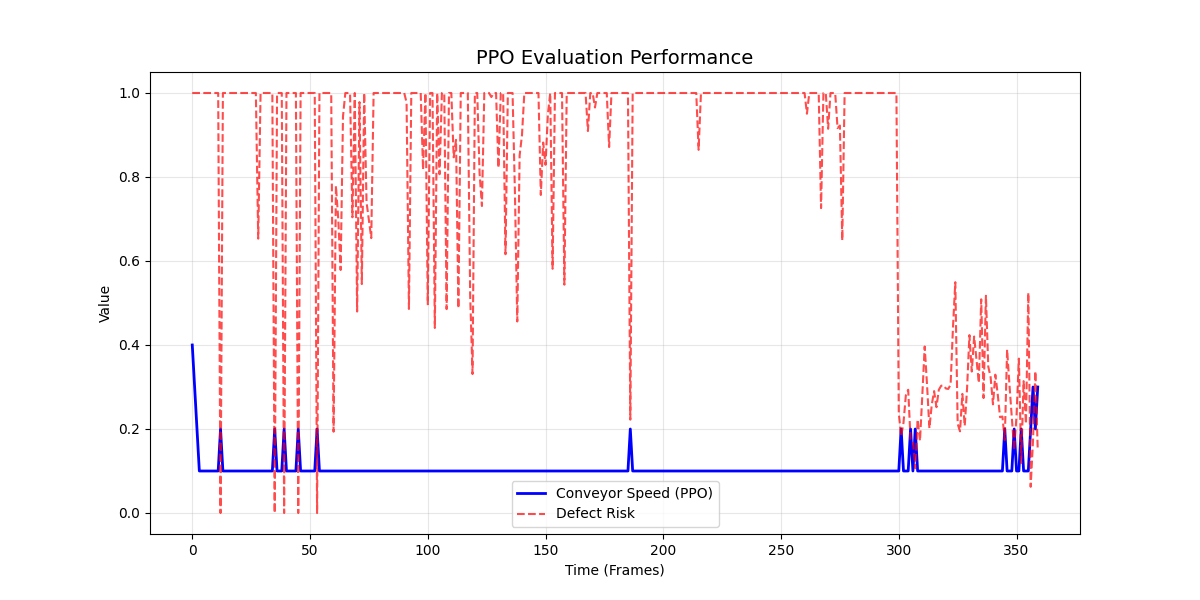
\includegraphics[width=0.8\linewidth]{img/ppo_performance_yolovn.png}
		\caption{تغییرات سرعت و ریسک برحسب طول فریم(\lr{yolov8n})}
	\end{figure}
	\begin{figure}[H]
		\centering
		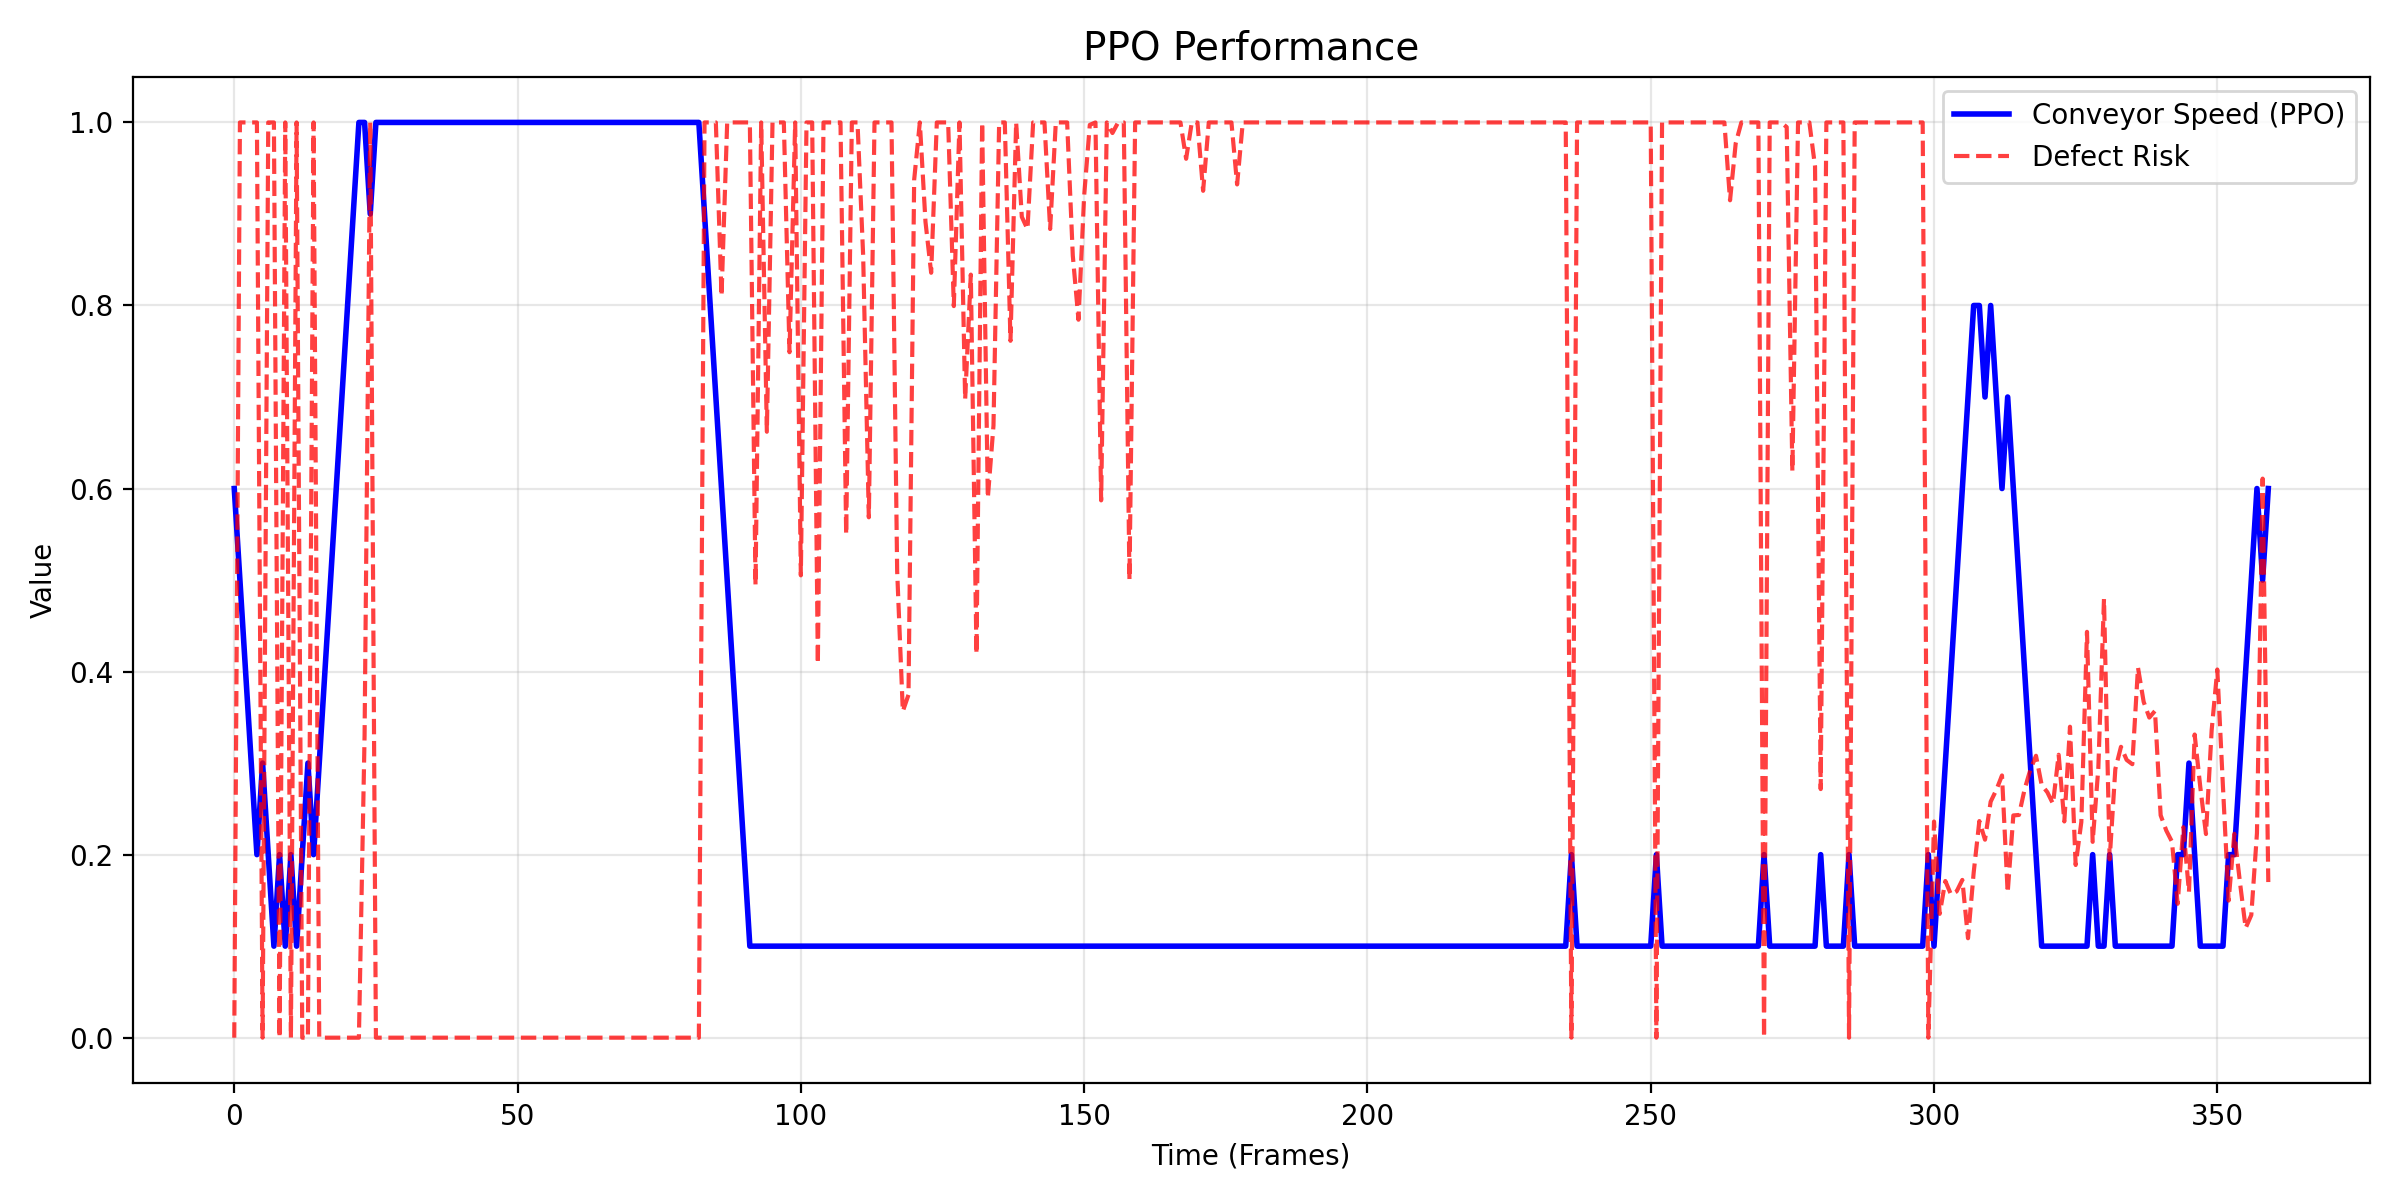
\includegraphics[width=0.8\linewidth]{img/ppo_performance_yolovimprove.png}
		\caption{تغییرات سرعت و ریسک برحسب طول فریم(\lr{yolov8n-Improvement})}
	\end{figure}
	\begin{figure}[H]
		\centering
		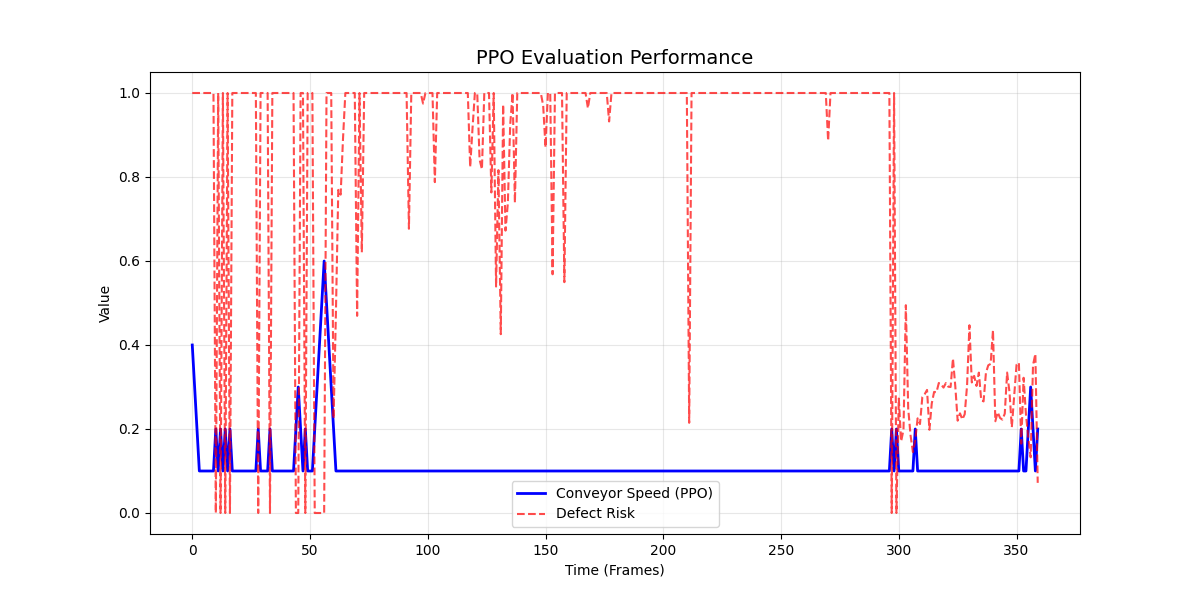
\includegraphics[width=0.8\linewidth]{img/ppo_performance_yolovgse.png}
		\caption{تغییرات سرعت و ریسک برحسب طول فریم(\lr{yolov8n-gse})}
	\end{figure}
	\begin{figure}[H]
		\centering
		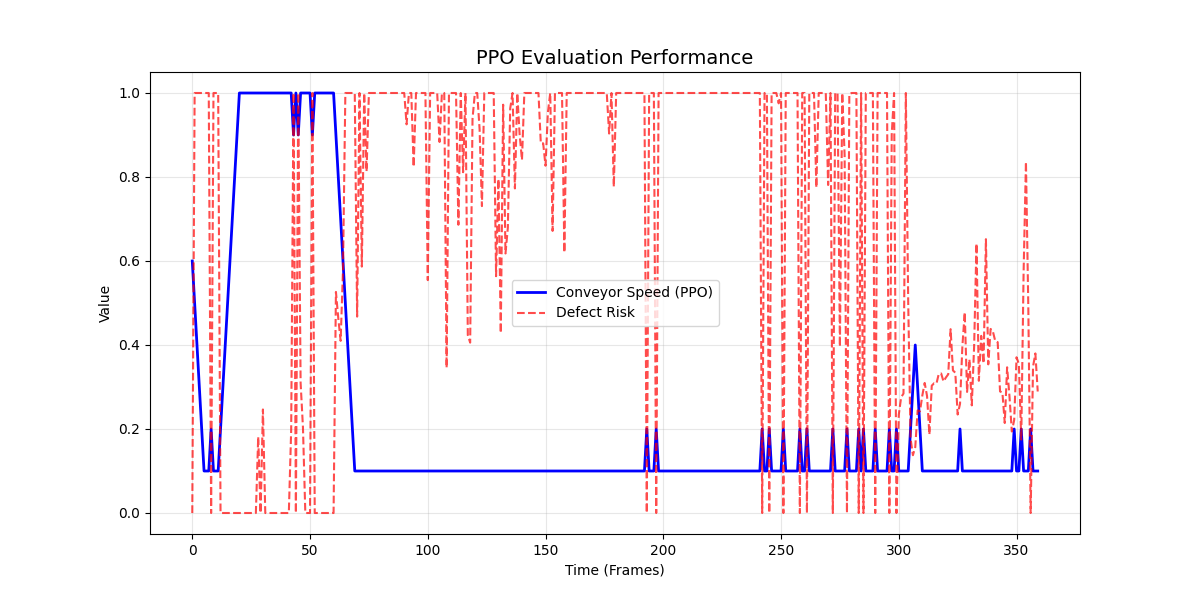
\includegraphics[width=0.8\linewidth]{img/ppo_performance_yolov11m.png}
		\caption{تغییرات سرعت و ریسک برحسب طول فریم(\lr{yolov11m}}
	\end{figure}
	
	
	\subsubsection*{تحلیل عملکرد مدل‌های آشکارسازی در حلقه کنترل}
	
	نتایج نشان دادند که کیفیت خروجی مدل آشکارسازی، اثر مستقیمی بر کیفیت تصمیم‌های عامل \lr{PPO} دارد. از میان چهار مدل مورد بررسی، استفاده از \lr{YOLOv8n-Improvement} بهترین عملکرد کنترلی را ایجاد کرد. علت این موضوع، کیفیت بالاتر تشخیص و طبقه‌بندی عیوب، پایداری بهتر خروجی‌ها روی داده‌های اعتبارسنجی و قابلیت اطمینان بیشتر ویژگی‌های ورودی عامل یادگیری تقویتی است.
	
	مدل \lr{YOLOv8n} استاندارد، به دلیل ضعف نسبی در تشخیص و تفکیک برخی کلاس‌های عیب، ورودی‌های کم‌دقت‌تری را به عامل کنترل ارائه می‌کرد. در نتیجه، برآورد ریسک و میانگین اطمینان در برخی فریم‌ها با عدم قطعیت بیشتری همراه بود و عامل \lr{PPO} نیز نتوانست سیاست کنترلی مطلوبی بیاموزد. این رفتار با نتایج پیاده‌سازی‌های پیشین کنترل مبتنی بر \lr{Qlearning} نیز سازگار بود؛ زیرا هرگونه خطا در تشخیص اولیه، به‌صورت مستقیم به زنجیره تصمیم‌گیری کنترلی منتقل می‌شود.
	
	مدل‌های \lr{YOLOv11m} و \lr{YOLOv8n-Improvement} به دلیل بهبود استخراج ویژگی و عملکرد مناسب‌تر در داده‌های اعتبارسنجی، ورودی‌های پایدارتر و معنادارتری برای عامل فراهم کردند. به‌ویژه، \lr{YOLOv8n-Improvement} توانست ضمن حفظ دقت تشخیص، ریسک را با نوسان کمتر و قابلیت اتکای بالاتر به عامل کنترل منتقل کند. بنابراین، رفتار سرعت نوار نقاله در این حالت منطقی‌تر، نرم‌تر و سازگارتر با وضعیت واقعی عیوب مشاهده شد.
	
	اگرچه \lr{YOLO11m} به دلیل ظرفیت بالاتر شبکه در برخی شاخص‌های آشکارسازی عملکرد مناسبی ارائه می‌دهد، افزایش تعداد پارامترها الزاماً به بهبود متناسب در حلقه کنترل منجر نشد. در مقابل، مدل‌ سفارشی سبک‌تر توانست مصالحه مطلوب‌تری میان کیفیت تشخیص، سرعت استنتاج و پایداری ورودی کنترل‌کننده برقرار کند.
	
	\subsubsection*{مقایسه رفتاری \lr{PPO} با روش‌های ساده‌تر یادگیری تقویتی}
	
	در مقایسه با روش‌های ساده‌تر یادگیری تقویتی استفاده‌شده در مراحل پیشین، عملکرد \lr{PPO} در هر چهار مدل تا حدی حساس‌تر به کیفیت پارامترها و ویژگی‌های ورودی بود. علت اصلی این مسئله آن است که \lr{PPO} از یک سیاست مبتنی بر شبکه عصبی چندلایه استفاده می‌کند و عملکرد آن به تنظیم مناسب ابرپارامترهایی مانند نرخ یادگیری، ضریب آنتروپی، محدوده برش سیاست، ساختار شبکه و طراحی تابع پاداش وابسته است.
	
	در صورتی که خروجی مرحله تشخیص شامل خطا، نوسان زیاد یا طبقه‌بندی نادرست باشد، این عدم قطعیت وارد فضای حالت عامل شده و یادگیری سیاست مناسب را دشوار می‌کند. به عبارت دیگر، \lr{PPO} به کیفیت داده و طراحی محیط حساس‌تر است؛ اما در مقابل، قادر است روابط غیرخطی و پیچیده‌تری را میان ریسک، اطمینان، سرعت و تصمیم کنترلی بیاموزد.
	
	روش‌های ساده‌تر یادگیری تقویتی با ساختار جدولی یا ماتریسی، در برخی شرایط نسبت به تغییرات محدود پارامترها حساسیت کمتری دارند، زیرا فضای تصمیم‌گیری آن‌ها ساده‌تر است. با این حال، این روش‌ها معمولاً توانایی کمتری برای مدل‌سازی روابط پیوسته و چندمتغیره دارند. بنابراین، عملکرد ضعیف‌تر نسبی \lr{PPO} در برخی آزمایش‌ها را باید ناشی از حساسیت بیشتر آن به کیفیت مدل آشکارسازی و تنظیمات آموزشی دانست، نه لزوماً ضعف ذاتی الگوریتم.
	
	\subsubsection*{جمع‌بندی}
	
	کنترل‌کننده مبتنی بر \lr{PPO} توانست با استفاده از خروجی مدل‌های آشکارسازی، سرعت نوار نقاله را به‌صورت تطبیقی تنظیم کند. ویژگی اصلی این روش، ایجاد یک تلاش کنترلی نرم و شیب‌دار است که از تغییرات ناگهانی سرعت جلوگیری می‌کند. اعمال گام سرعتی $0.1$، جریمه تغییرات سرعت و ماهیت بهینه‌سازی بازده تجمعی در \lr{PPO} موجب شدند عامل مانند یک سازوکار پایین‌گذر عمل کرده و اثر پیک‌های لحظه‌ای ریسک را کاهش دهد.
	
	در میان مدل‌های ارزیابی‌شده، \lr{YOLOv8n-Improvement} بهترین ورودی را برای کنترل‌کننده فراهم کرد و در نتیجه، مناسب‌ترین رفتار سرعت و ریسک را نشان داد. این نتایج بیانگر آن هستند که در یک سامانه کنترل مبتنی بر بینایی ماشین، افزایش پیچیدگی مدل آشکارسازی به‌تنهایی کافی نیست؛ بلکه پایداری، دقت طبقه‌بندی، کیفیت برآورد ریسک و سرعت استنتاج نیز نقش تعیین‌کننده‌ای در عملکرد نهایی حلقه کنترل دارند.
	
	\section{بنچمارک محاسباتی و تحلیل تریدآف دقت--سرعت}
	
	به‌منظور ارزیابی عملی روش‌های کنترلی، بنچمارک نهایی برای چهار مدل
	\lr{YOLOv8n}، \lr{YOLOv8n-GSE}، \lr{YOLOv8n-Improvement} و \lr{YOLO11m}
	در ترکیب با عامل کنترلی مبتنی بر \lr{PPO} انجام شد. نتایج این ارزیابی در دو
	بستر سخت‌افزاری شامل پردازش روی \lr{CPU} و پردازش شتاب‌گرفته با \lr{GPU}
	ثبت شده‌اند. معیارهای اصلی مقایسه شامل سرعت پردازش یا نرخ فریم
	(\lr{FPS})، سرعت میانگین نوار نقاله، و معیارهای مرتبط با ریسک تشخیص عیب
	هستند.
	
	\begin{figure}[h!]
		\centering
		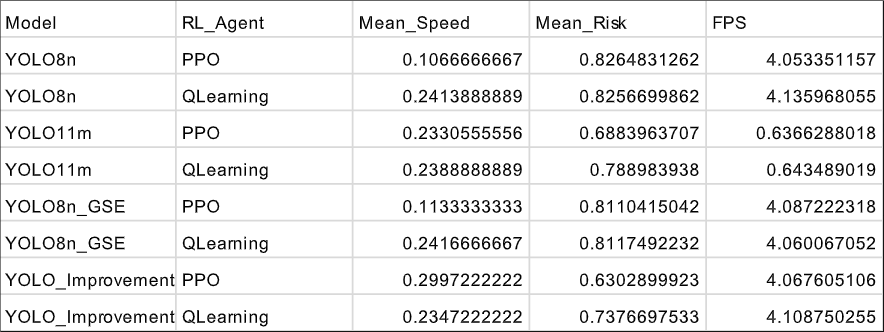
\includegraphics[width=0.9\linewidth]{img/cpu.png}
		\caption{نتایج بنچمارک پیاده سازی در بستر \lr{CPU}}
		\label{fig:ppo-benchmark-1}
	\end{figure}
	
	\begin{figure}[h!]
		\centering
		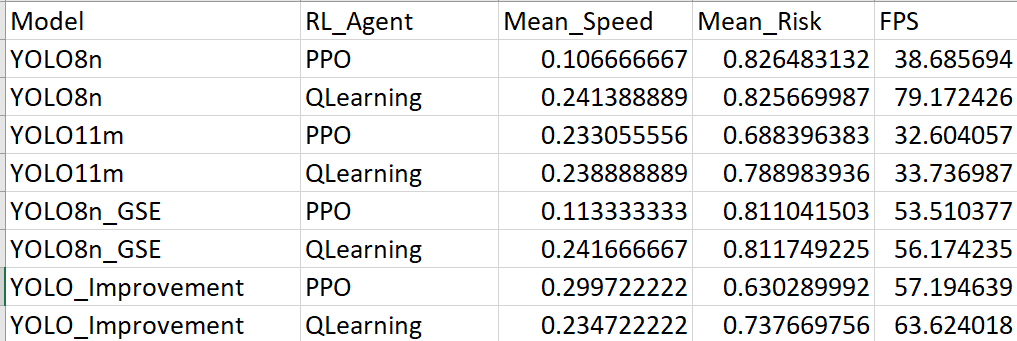
\includegraphics[width=0.9\linewidth]{img/gpu.png}
		\caption{نتایج بنچمارک پیاده سازی در بستر \lr{GPU}}
		\label{fig:ppo-benchmark-2}
	\end{figure}
	
	\subsection{تحلیل سربار محاسباتی عامل \lr{PPO}}
	
	در مقایسه با روش‌های جدولی مانند \lr{Q-Learning}، پیاده‌سازی مبتنی بر
	\lr{PPO} دارای سربار محاسباتی اندکی بیشتر است. در روش‌های جدولی، تصمیم
	کنترلی عموماً با مراجعه به یک جدول یا ماتریس حالت--عمل انجام می‌شود؛ ازاین‌رو
	فرایند انتخاب عمل ساده‌تر بوده و هزینه محاسباتی بسیار کمی دارد. در مقابل،
	عامل \lr{PPO} از سیاست مبتنی بر شبکه عصبی چندلایه
	(\lr{MLP Policy}) استفاده می‌کند. بنابراین، در هر گام کنترل، علاوه بر
	استنتاج مدل \lr{YOLO}، یک مرحله عبور رو به جلو از شبکه سیاست نیز برای
	انتخاب عمل مناسب انجام می‌شود.
	
	این موضوع باعث کاهش محدود نرخ \lr{FPS} نسبت به کنترل‌کننده‌های جدولی
	می‌شود؛ با این حال، میزان این کاهش در مقایسه با هزینه اصلی استنتاج مدل
	آشکارسازی زیاد نیست. مزیت این سربار محدود آن است که عامل \lr{PPO} قادر
	است ارتباط‌های غیرخطی میان ریسک عیب، اطمینان آشکارسازی، سرعت فعلی،
	تعداد عیوب و خروجی کنترل‌کننده فازی را یاد بگیرد. بنابراین، کاهش جزئی
	سرعت پردازش در ازای ایجاد رفتار کنترلی نرم‌تر و تصمیم‌گیری منعطف‌تر،
	قابل توجیه است.
	
	\subsection{مقایسه مدل‌ها از دیدگاه سرعت و دقت}
	
	نتایج بنچمارک نشان می‌دهند که مدل \lr{YOLOv8n-Improvement} مناسب‌ترین
	توازن میان سرعت استنتاج، کیفیت ویژگی‌های ورودی عامل و مدیریت ریسک را
	ایجاد کرده است. این مدل، برخلاف مدل‌های بزرگ‌تر، سربار محاسباتی بسیار
	سنگینی ایجاد نمی‌کند و در عین حال، خروجی تشخیص پایدارتر و دقیق‌تری را برای
	عامل \lr{PPO} فراهم می‌سازد. در نتیجه، عامل کنترل می‌تواند با اطمینان
	بیشتری سرعت نوار نقاله را تنظیم کرده و در شرایط پرریسک، رفتار محافظه‌کارانه
	و در شرایط کم‌ریسک، رفتار بهره‌ورانه‌تری داشته باشد.
	
	مدل \lr{YOLO11m} به دلیل ابعاد بزرگ‌تر شبکه و تعداد پارامترهای بیشتر،
	هزینه استنتاج بالاتری دارد. همان‌طور که در نتایج بنچمارک نیز مشاهده
	می‌شود، استفاده از این مدل باعث کاهش محسوس نرخ \lr{FPS} شده است. اگرچه
	ظرفیت بالاتر این مدل می‌تواند در برخی شرایط به بهبود تشخیص منجر شود،
	اما این بهبود لزوماً متناسب با افت سرعت و هزینه محاسباتی ایجادشده نیست.
	ازاین‌رو، \lr{YOLO11m} برای سناریوهایی که محدودیت سخت‌گیرانه بی‌درنگ
	ندارند مناسب‌تر است، در حالی که برای کنترل سرعت نوار نقاله در کاربردهای
	صنعتی برخط، مدل سبک‌تر و بهینه‌تر ارجحیت دارد.
	
	مدل پایه \lr{YOLOv8n} از نظر محاسباتی سبک است، اما به دلیل کیفیت پایین‌تر
	در طبقه‌بندی و تشخیص برخی عیوب، ویژگی‌های ریسک کم‌اعتماد‌تری به عامل
	کنترلی منتقل می‌کند. بنابراین، سرعت بالاتر این مدل به‌تنهایی به معنای
	عملکرد کنترلی بهتر نیست. مدل \lr{YOLOv8n-GSE} نسبت به نسخه پایه بهبود
	ایجاد می‌کند، اما بر اساس نتایج نهایی، مدل \lr{YOLOv8n-Improvement} بهترین
	مصالحه میان هزینه پردازش و دقت موردنیاز در حلقه کنترل را ارائه می‌دهد.
	
	\subsection{اثر بستر سخت‌افزاری \lr{CPU} و \lr{GPU}}
	
	ارزیابی‌ها هم روی \lr{CPU} و هم روی \lr{GPU} انجام شده‌اند تا وابستگی
	عملکرد سامانه به سخت‌افزار مشخص شود. در حالت \lr{CPU}، اختلاف هزینه
	محاسباتی مدل‌ها، به‌ویژه برای مدل بزرگ‌تر \lr{YOLO11m}، آشکارتر است و نرخ
	فریم کاهش بیشتری پیدا می‌کند. در مقابل، استفاده از \lr{GPU} زمان استنتاج
	مدل آشکارسازی و شبکه سیاست \lr{PPO} را کاهش داده و نرخ پردازش را بهبود
	می‌دهد.
	
	با وجود این، روند مقایسه مدل‌ها در هر دو بستر تقریباً یکسان است: مدل‌های
	سنگین‌تر به منابع محاسباتی بیشتری نیاز دارند و مدل
	\lr{YOLOv8n-Improvement} توازن مناسب‌تری میان دقت و سرعت حفظ می‌کند.
	بنابراین، استفاده از \lr{GPU} برای پیاده‌سازی صنعتی با نرخ فریم بالا
	توصیه می‌شود؛ اما حتی در محیط‌های محدودتر مبتنی بر \lr{CPU} نیز انتخاب
	یک معماری بهینه مانند \lr{YOLOv8n-Improvement} می‌تواند عملکرد قابل قبولی
	فراهم کند.
	
	\subsection{جمع‌بندی}
	
	به‌طور کلی، عامل \lr{PPO} نسبت به روش‌های جدولی، به دلیل استفاده از شبکه
	عصبی، سربار محاسباتی بیشتری دارد؛ اما این سربار محدود بوده و در مقابل،
	قابلیت مدل‌سازی روابط پیچیده و تولید تلاش کنترلی نرم را فراهم می‌کند.
	نتایج بنچمارک نشان می‌دهند که \lr{YOLOv8n-Improvement} بهترین گزینه برای
	ترکیب با عامل \lr{PPO} است، زیرا ضمن حفظ سرعت مناسب، دقت تشخیص و کیفیت
	برآورد ریسک لازم برای کنترل تطبیقی و پایدار نوار نقاله را تأمین می‌کند.
	
	
	\section{ارزیابی روش \lr{Model Soup} بر پایه مدل \lr{YOLOv8n-Improvement}}
	
	پس از بررسی مدل‌های مختلف در بخش‌های پیشین، مدل \lr{YOLOv8n-Improvement} به‌عنوان
	مدل پایه برای اجرای روش \lr{Model Soup} انتخاب شد. دلیل این انتخاب، عملکرد
	بهتر این مدل نسبت به سایر مدل‌های بررسی‌شده، از جمله \lr{YOLOv8n}،
	\lr{YOLOv8n-GSE} و \lr{YOLO11m}، از دیدگاه تعادل میان دقت تشخیص، مقاومت
	در برابر بیش‌برازش و هزینه محاسباتی بود. هدف از به‌کارگیری \lr{Model Soup}
	این بود که دانش تخصصی مدل‌های آموزش‌دیده برای کلاس‌های مختلف عیب سطحی
	با یکدیگر ترکیب شود و یک مدل نهایی با قابلیت تعمیم بهتر ایجاد گردد.
	
	\subsection{آماده‌سازی داده‌ها و تعریف مسئله}
	
	دیتاست مورد استفاده شامل شش کلاس عیب سطحی شامل \lr{crazing}،
	\lr{inclusion}، \lr{patches}، \lr{pitted\_surface}،
	\lr{rolled-in\_scale} و \lr{scratches} است. ابتدا فایل پیکربندی داده‌ها
	برای مسئله شش‌کلاسه تعریف شد تا مسیرهای داده‌های آموزش و اعتبارسنجی، تعداد
	کلاس‌ها و نام هر کلاس در اختیار چارچوب \lr{Ultralytics} قرار گیرد.
	
	برای ایجاد مدل‌های خبره، داده‌ها به‌صورت کلاس‌محور پردازش شدند. به این
	صورت که برای هر کلاس، یک مجموعه برچسب اختصاصی ساخته شد و تنها نمونه‌های
	مربوط به همان کلاس در فایل‌های برچسب نگه داشته شدند. تصاویر اصلی میان همه
	مدل‌های خبره مشترک باقی ماندند و برای جلوگیری از تکثیر غیرضروری داده‌ها،
	از پیوند نمادین (\lr{Symbolic Link}) برای اتصال پوشه تصاویر استفاده شد.
	بنابراین، برای هر کلاس یک مجموعه داده موقت شامل تصاویر مشترک و برچسب‌های
	فیلترشده همان کلاس ایجاد شد.
	
	این راهبرد باعث می‌شود هر مدل خبره در فرایند آموزش، تمرکز بیشتری بر
	ویژگی‌های بصری عیب هدف داشته باشد. برای مثال، مدل خبره مربوط به کلاس
	\lr{crazing} عمدتاً الگوهای ترک‌مانند، خطوط ریز و ساختارهای نامنظم سطح را
	یاد می‌گیرد؛ در حالی که مدل خبره کلاس \lr{pitted\_surface} بر فرورفتگی‌ها،
	نقاط تیره و ناهمواری‌های موضعی سطح تمرکز بیشتری خواهد داشت.
	
	\subsection{معماری مدل خبره}
	
	مدل‌های خبره بر مبنای معماری سفارشی \lr{YOLOv8n-Improvement} ساخته شدند.
	
	\subsection{آموزش مدل‌های خبره}
	
	برای هر یک از شش کلاس، یک مدل خبره مستقل با معماری سفارشی آموزش داده شد.
	هر مدل با اندازه ورودی \(640\times640\)، اندازه دسته \(16\)، و حداکثر
	\(50\) دوره آموزش آموزش دید. بهینه‌ساز \lr{AdamW} با نرخ یادگیری اولیه
	\(10^{-3}\) استفاده شد. همچنین، از برنامه کاهش نرخ یادگیری کسینوسی
	(\lr{Cosine Learning Rate Schedule})، پنج دوره گرم‌سازی
	(\lr{Warm-up}) و ضریب نرخ یادگیری نهایی \(0.01\) استفاده شد.
	
	برای جلوگیری از ایجاد نمونه‌های مصنوعی نامتناسب با ساختار واقعی عیوب
	فلزی، افزایش‌داده‌های \lr{Mosaic}، \lr{Mixup} و \lr{CutMix} غیرفعال
	شدند. در مقابل، وارونگی افقی و عمودی با احتمال \(0.5\) و تغییر مقیاس
	با ضریب \(0.3\) اعمال شد. از آنجا که رنگ در دیتاست مورد استفاده نقش اصلی
	ندارد و تمرکز مسئله بر الگوهای بافتی سطح است، تغییرات فضای رنگی
	\lr{HSV} نیز غیرفعال در نظر گرفته شد.
	
	به‌منظور جلوگیری از آموزش تکراری، پیش از آموزش هر مدل خبره بررسی شد که
	آیا فایل وزن بهینه آن موجود است یا خیر. در صورت وجود وزن \lr{best.pt}،
	آموزش آن مدل نادیده گرفته شده و همان وزن از پیش آموزش‌دیده در مرحله ساخت
	\lr{Model Soup} استفاده شد.
	
	\subsection{ساخت مدل نهایی با روش \lr{Model Soup}}
	
	پس از آموزش شش مدل خبره، وزن‌های ذخیره‌شده آن‌ها بارگذاری شدند. روش مورد
	استفاده برای ساخت \lr{Model Soup}، میانگین‌گیری مستقیم پارامترهای مدل‌ها
	بود. اگر \(\theta_i\) بردار پارامترهای مدل خبره مربوط به کلاس \(i\) باشد،
	پارامترهای مدل نهایی مطابق رابطه زیر محاسبه شدند:
	
	\[
	\theta_{\text{soup}} =
	\frac{1}{N}\sum_{i=1}^{N}\theta_i,
	\qquad N=6
	\]
	
	در این فرایند، تنها پارامترهای اعشاری مدل‌ها میانگین‌گیری شدند و ساختار
	شبکه نهایی از روی یکی از مدل‌های خبره بارگذاری شد تا تعداد کلاس‌ها و
	ساختار سر آشکارسازی مدل به‌درستی حفظ شود. سپس وزن‌های میانگین‌گیری‌شده
	در مدل نهایی قرار گرفتند و مدل با نام \lr{model\_soup\_final.pt} ذخیره شد.
	
	ایده اصلی این روش آن است که هر مدل خبره بخشی از دانش مربوط به یک نوع عیب
	را آموخته است و میانگین‌گیری وزن‌ها ممکن است به مدلی منجر شود که دانش
	مدل‌های مختلف را به‌صورت هم‌زمان حفظ کند. با این حال، میانگین‌گیری مستقیم
	تمام وزن‌ها، به‌ویژه وزن‌های سر آشکارسازی (\lr{Detection Head})، الزاماً
	بهترین روش ترکیب مدل‌های تخصصی نیست؛ زیرا هر سر آشکارسازی در طول آموزش
	بیشتر به ویژگی‌های یک کلاس خاص سازگار شده است.
	
	\subsection{ارزیابی مدل نهایی روی داده‌های اعتبارسنجی}
	
	پس از ساخت مدل نهایی، ارزیابی روی مجموعه اعتبارسنجی انجام شد. برای بررسی
	اثر آستانه اطمینان، سه مقدار \(0.3\)، \(0.4\) و \(0.5\) آزمایش شدند.
	در هر ارزیابی، منحنی‌های عملکرد، فایل‌های پیش‌بینی، مقادیر اطمینان،
	خروجی \lr{JSON} و ماتریس‌های درهم‌ریختگی ذخیره شدند. معیارهای اصلی
	ارزیابی شامل دقت (\lr{Precision})، بازخوانی (\lr{Recall})،
	\lr{mAP@50} و \lr{mAP@50-95} بودند.
	
	بر اساس بررسی‌های انجام‌شده، مدل در بازه آستانه اطمینان حدود
	\(0.25\) تا \(0.3\) عملکرد متعادل‌تری داشت. در این بازه، تعداد قابل قبولی
	از عیوب شناسایی می‌شوند، در حالی که نرخ پیش‌بینی‌های نادرست نیز به‌طور
	کامل افزایش نمی‌یابد. ازاین‌رو، آستانه اطمینان \(0.3\) به‌عنوان آستانه
	اصلی برای ارائه نتایج مدل \lr{Model Soup} انتخاب شد.
	
	\subsubsection*{نتایج کمی مدل \lr{Model Soup}}
	
	نتایج ارزیابی در آستانه اطمینان \(0.3\) در شکل ارائه‌شده نشان می‌دهد که
	مدل روی کل مجموعه اعتبارسنجی شامل \(360\) تصویر و \(854\) نمونه عیب،
	به مقادیر \lr{Precision} برابر با \(0.663\)، \lr{Recall} برابر با
	\(0.587\)، \lr{mAP@50} برابر با \(0.523\) و \lr{mAP@50-95} برابر با
	\(0.266\) دست یافته است.
	
	بررسی کلاس‌به‌کلاس نشان می‌دهد که کلاس \lr{patches} بهترین عملکرد را
	دارد و به مقادیر \lr{Precision} برابر با \(0.794\)، \lr{Recall} برابر
	با \(0.839\)، \lr{mAP@50} برابر با \(0.802\) و \lr{mAP@50-95} برابر با
	\(0.493\) رسیده است. پس از آن، کلاس‌های \lr{inclusion} و
	\lr{pitted\_surface} نیز عملکرد قابل قبولی دارند. به‌ترتیب، مقدار
	\lr{mAP@50} برای این دو کلاس برابر با \(0.684\) و \(0.650\) است.
	
	در مقابل، عملکرد مدل در تشخیص کلاس \lr{rolled-in\_scale} ضعیف‌تر است؛
	به‌طوری‌که مقدار \lr{mAP@50} آن برابر با \(0.338\) و مقدار
	\lr{mAP@50-95} آن برابر با \(0.114\) است. همچنین، کلاس \lr{crazing}
	با وجود \lr{Precision} برابر با \(0.583\)، دارای \lr{Recall} بسیار
	پایین \(0.130\) است. این نتیجه نشان می‌دهد که مدل تنها بخشی از نمونه‌های
	این کلاس را شناسایی کرده و تعداد قابل توجهی از ترک‌های ریز یا الگوهای
	مشابه ترک را از دست داده است. ماهیت ظریف، پراکنده و کم‌کنتراست عیوب
	\lr{crazing} می‌تواند یکی از دلایل اصلی این مسئله باشد.
	
	\begin{figure}[h!]
		\centering
		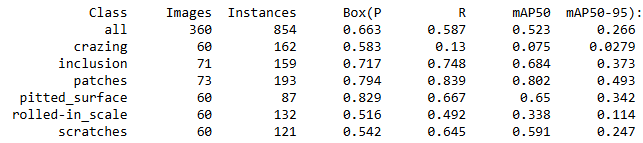
\includegraphics[width=0.88\linewidth]{img/results_soup.png}
		\caption{خلاصه نتایج ارزیابی مدل \lr{Model Soup} در آستانه اطمینان
			\(0.3\) روی مجموعه اعتبارسنجی.}
		\label{fig:soup-results-summary}
	\end{figure}
	
	\subsubsection*{تحلیل ماتریس‌های درهم‌ریختگی}
	
	برای تحلیل دقیق‌تر خطاهای طبقه‌بندی و آشکارسازی، ماتریس درهم‌ریختگی عادی
	و نسخه نرمال‌شده آن در شکل‌های \ref{fig:soup-confusion} و
	\ref{fig:soup-confusion-normalized} قرار می‌گیرند. ماتریس عادی تعداد
	واقعی پیش‌بینی‌ها و خطاها را نمایش می‌دهد؛ در حالی که ماتریس نرمال‌شده
	امکان مقایسه بهتر نرخ خطای کلاس‌ها را، مستقل از تعداد نمونه‌های هر کلاس،
	فراهم می‌کند.
	
	\begin{figure}[h!]
		\centering
		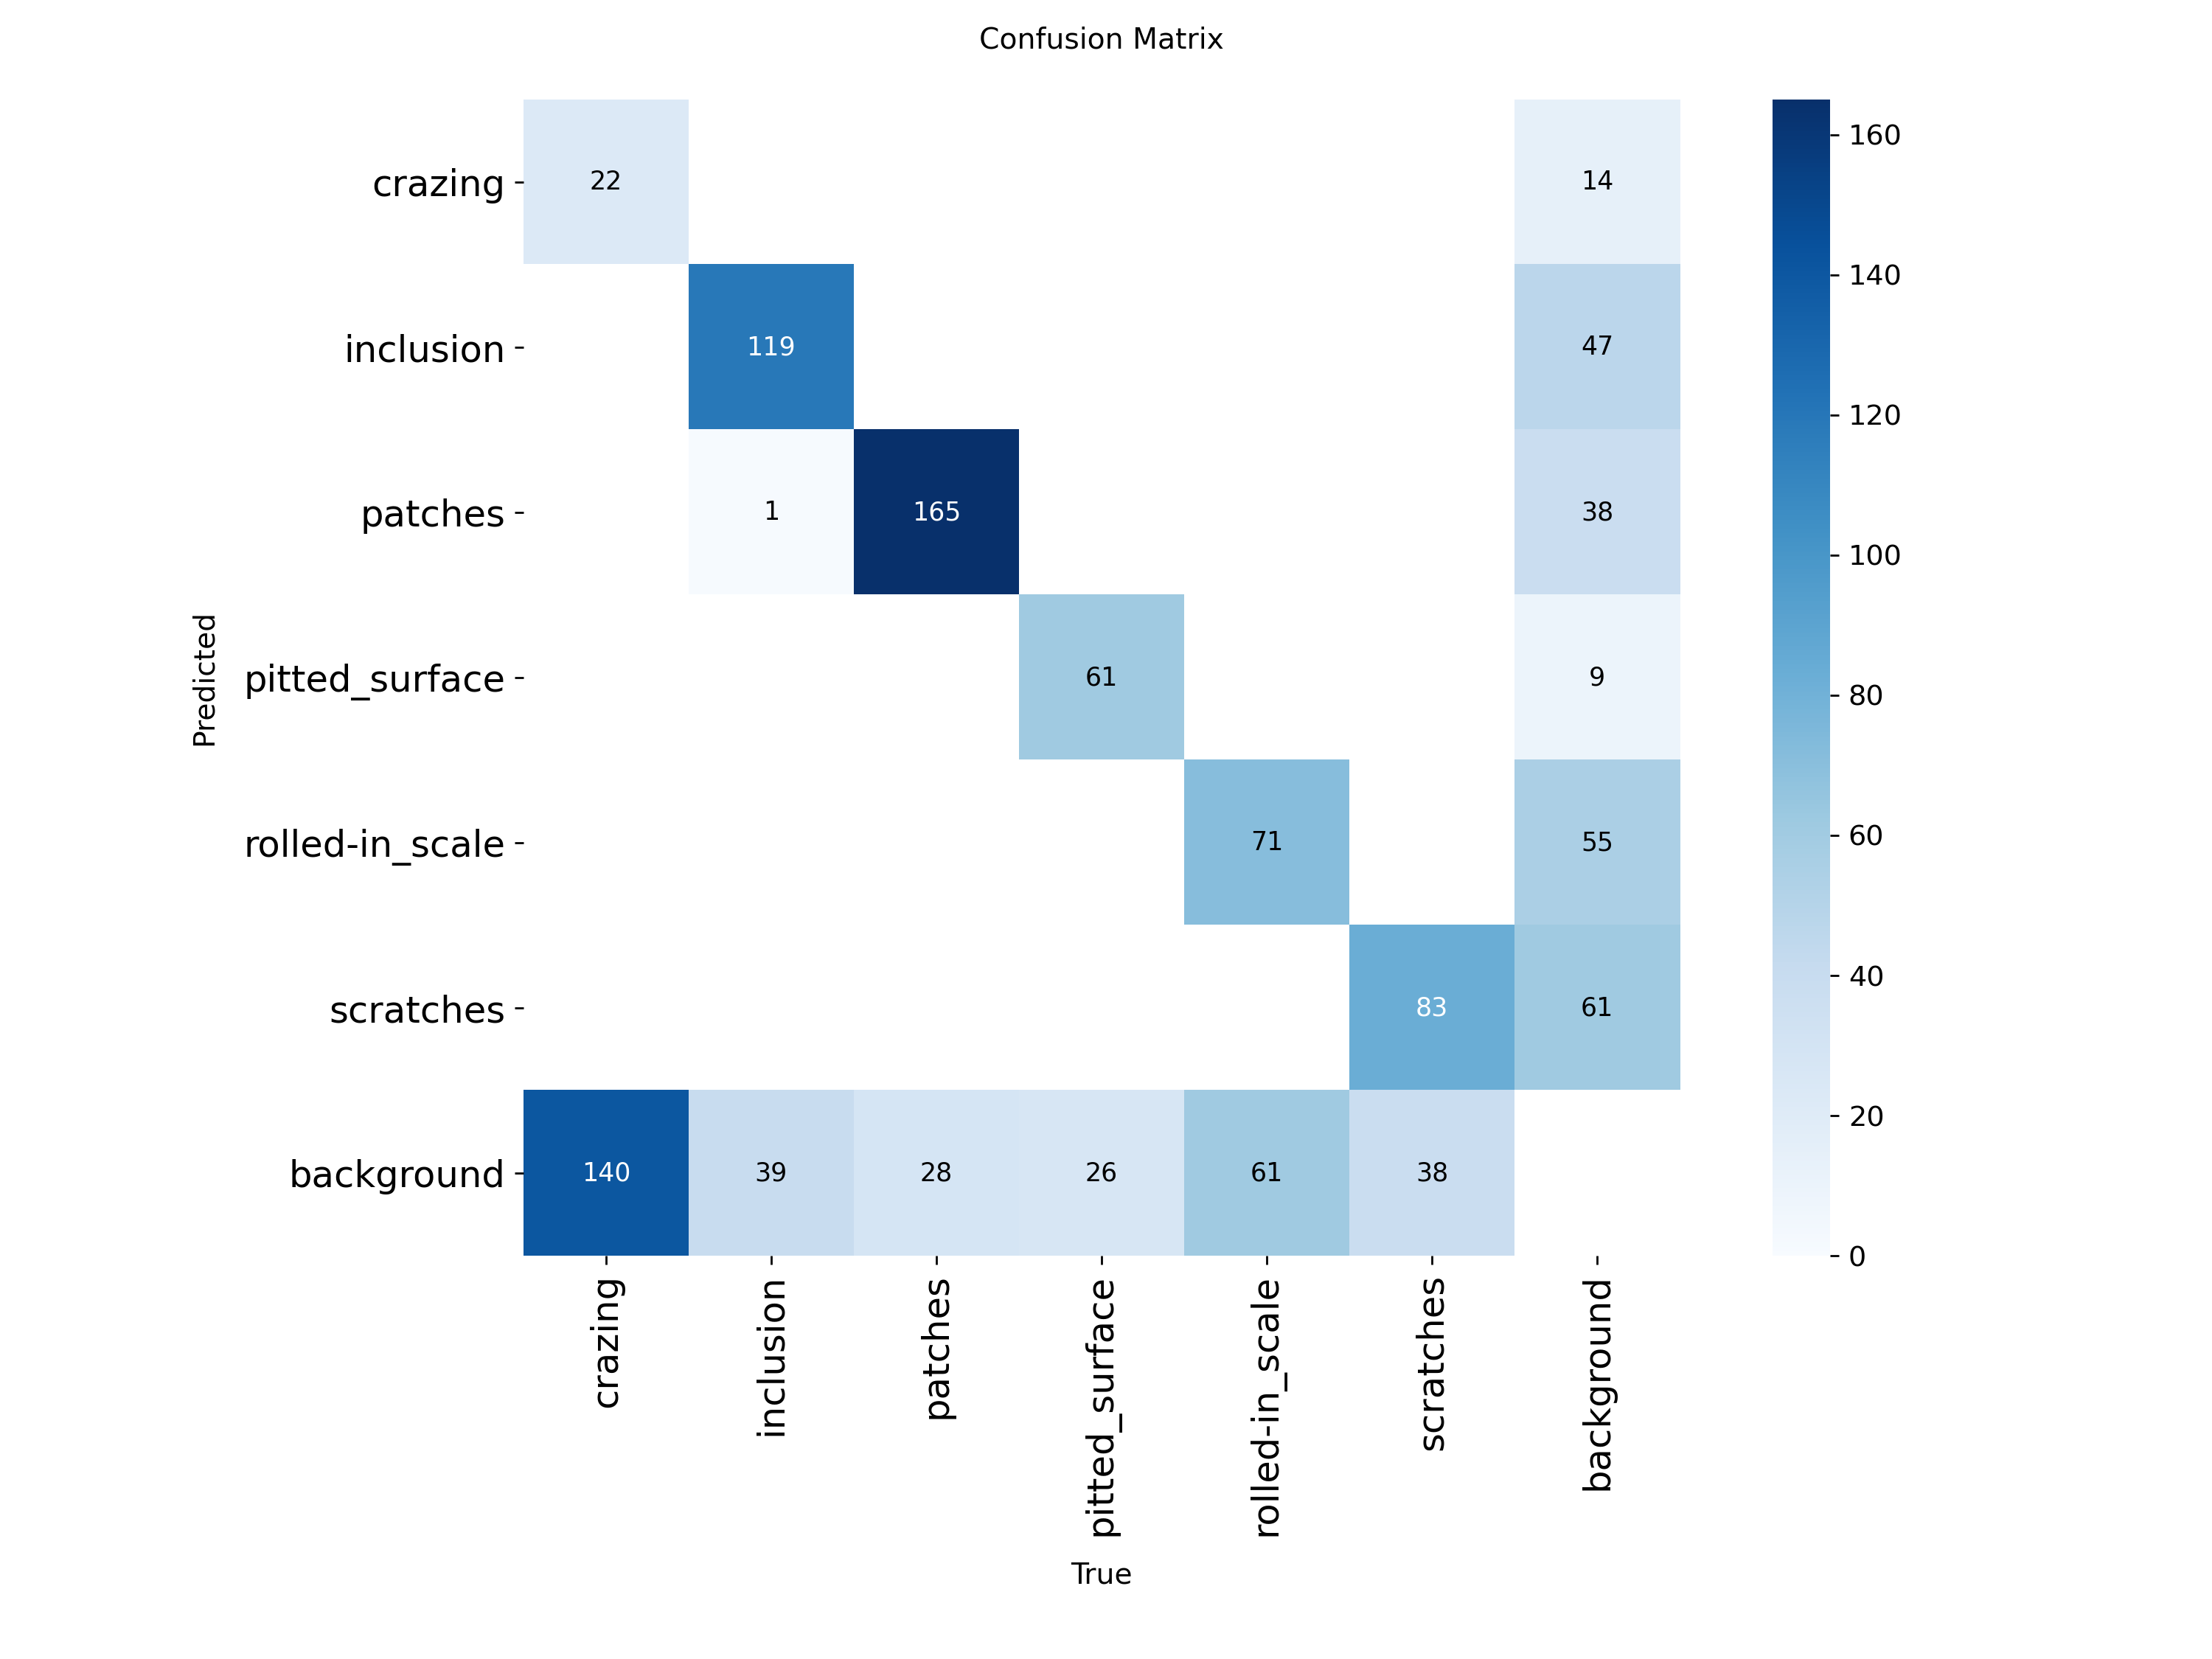
\includegraphics[width=0.5\linewidth]{img/confusion_matrix_soup.png}
		\caption{ماتریس درهم‌ریختگی مدل \lr{Model Soup} روی داده‌های
			اعتبارسنجی در آستانه اطمینان \(0.3\).}
		\label{fig:soup-confusion}
	\end{figure}
	
	\begin{figure}[h!]
		\centering
		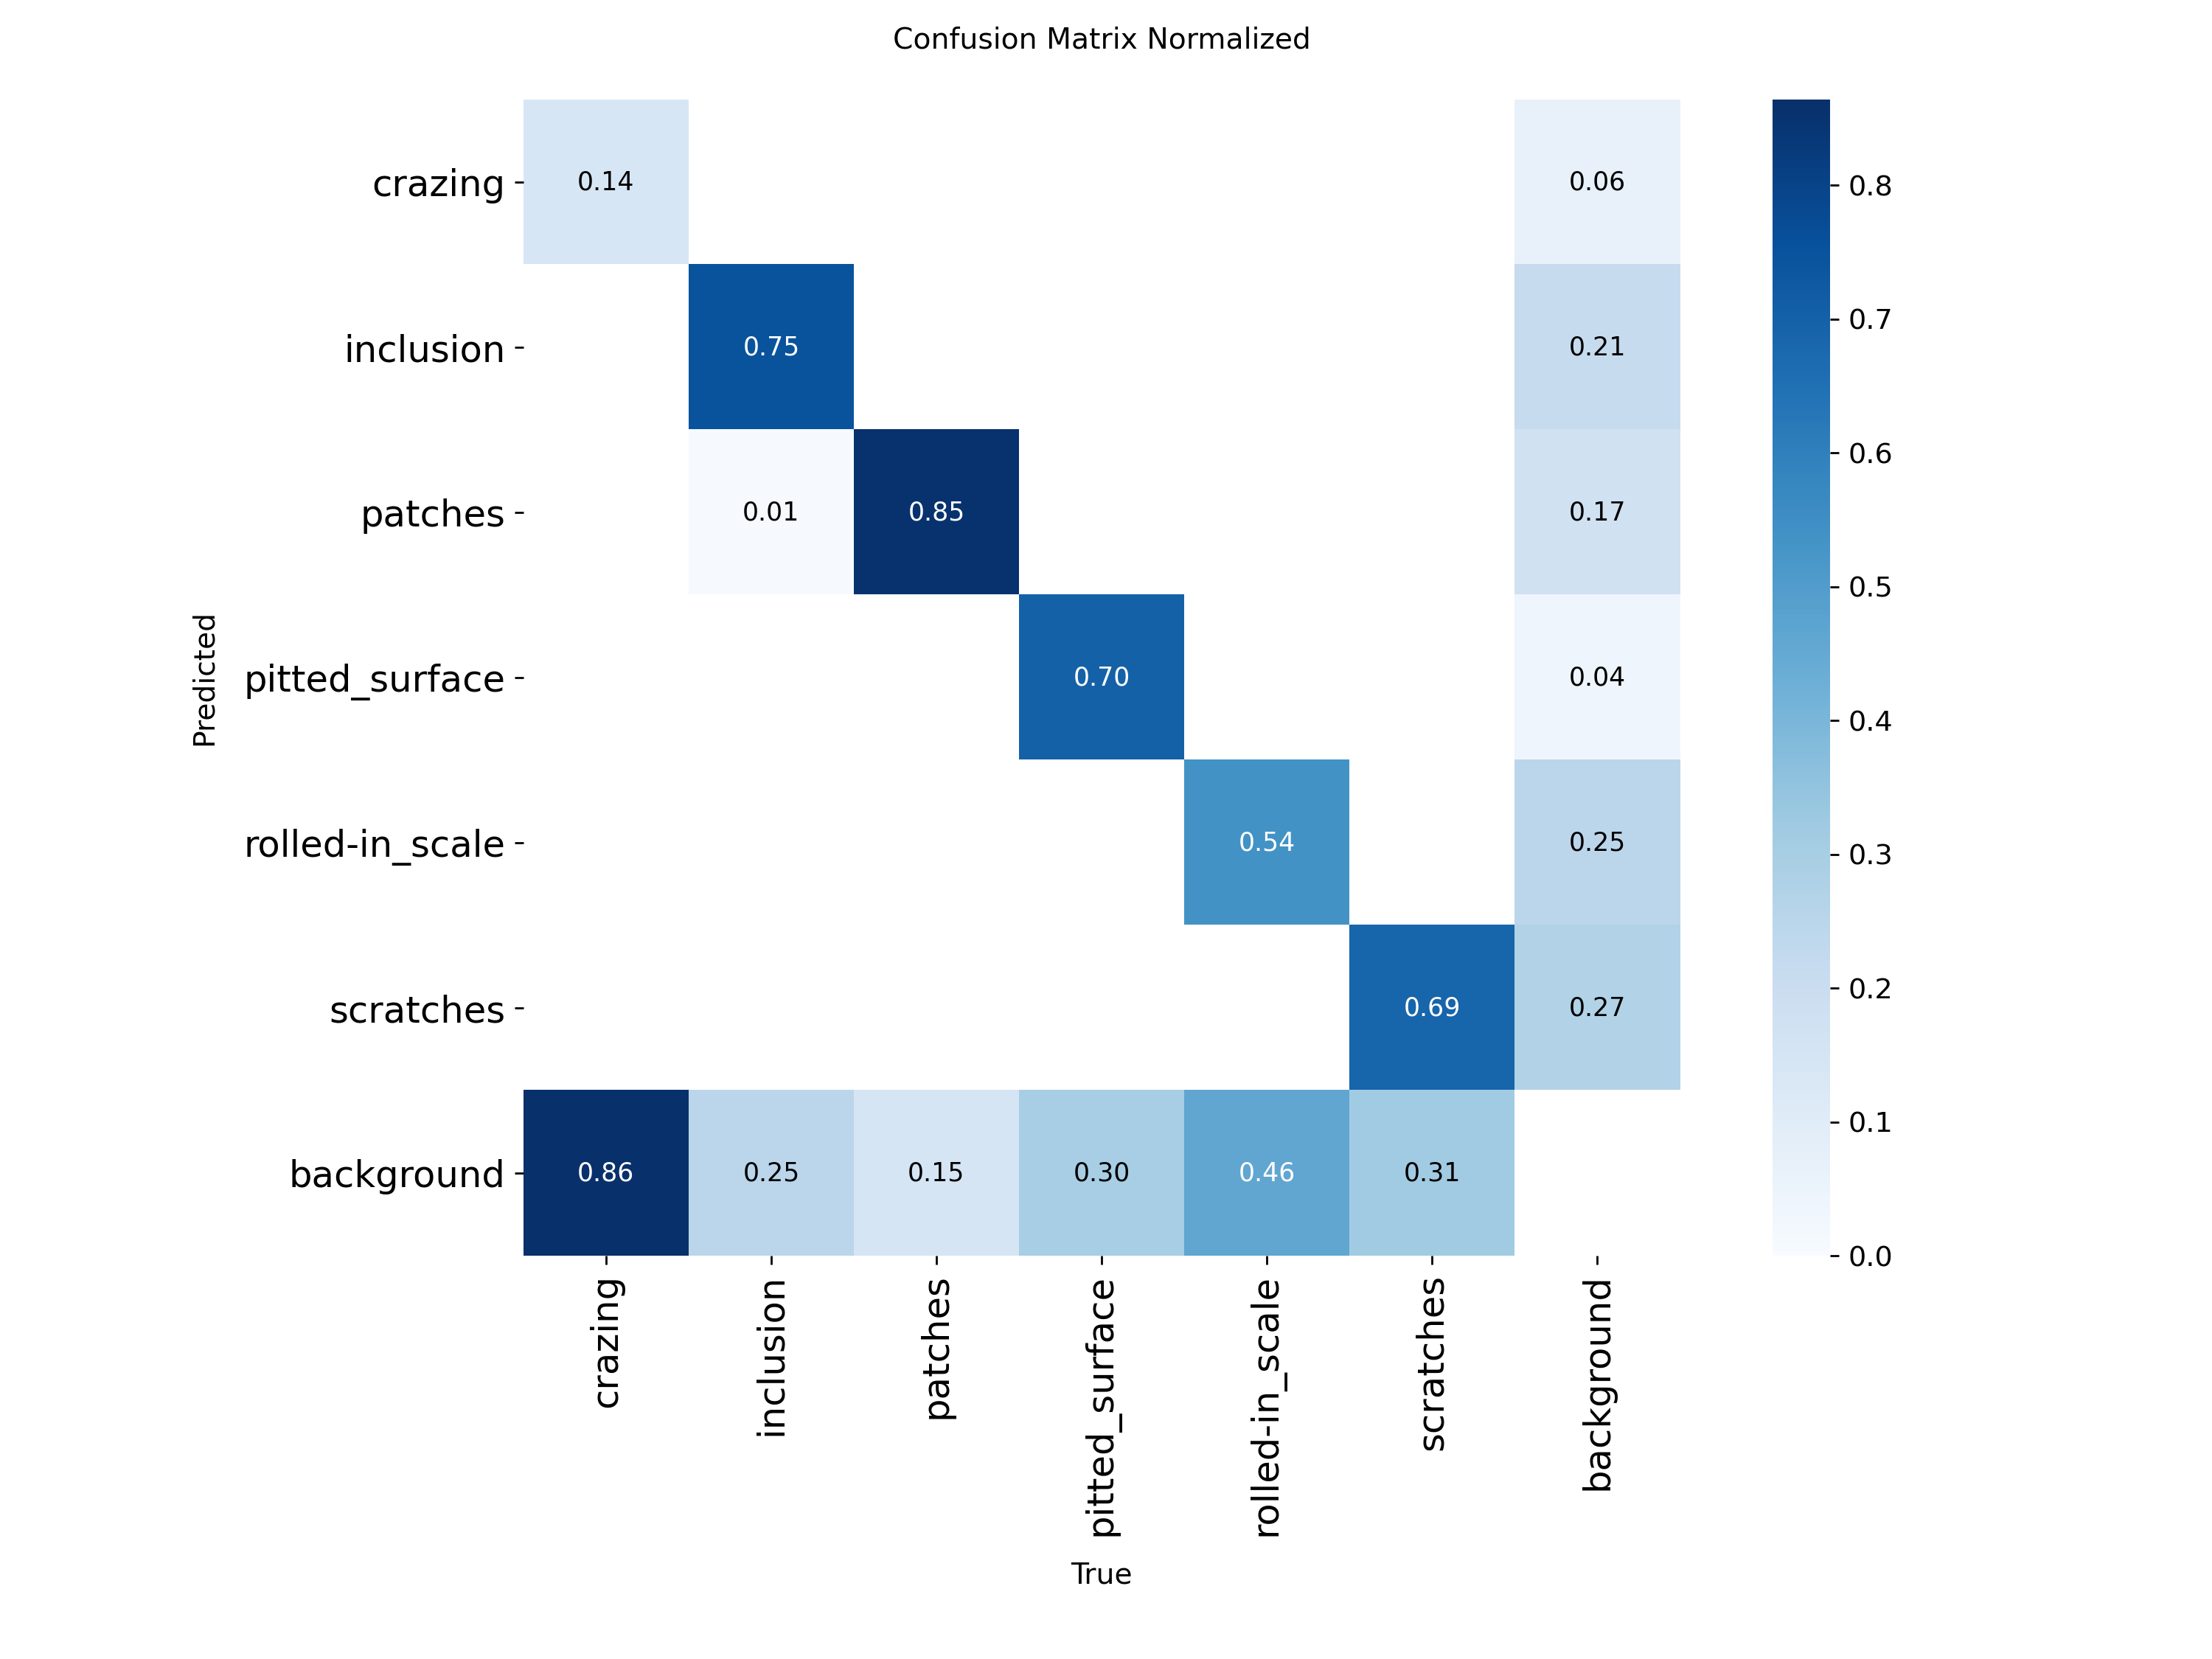
\includegraphics[width=0.5\linewidth]{img/confusion_matrix_normalized_soup.png}
		\caption{ماتریس درهم‌ریختگی نرمال‌شده مدل \lr{Model Soup} روی داده‌های
			اعتبارسنجی در آستانه اطمینان \(0.3\).}
		\label{fig:soup-confusion-normalized}
	\end{figure}
	\newpage
	\subsubsection*{تحلیل منحنی‌های عملکرد}
	
	برای بررسی رفتار مدل در آستانه‌های اطمینان مختلف، منحنی‌های
	\lr{F1-Confidence}، \lr{Precision-Confidence}،
	\lr{Recall-Confidence} و \lr{Precision-Recall} در شکل
	\ref{fig:soup-performance-curves} ارائه می‌شوند. این منحنی‌ها نشان
	می‌دهند که انتخاب آستانه \(0.3\) یک مصالحه مناسب میان دقت و بازخوانی
	ایجاد می‌کند. با افزایش آستانه، اگرچه دقت برخی پیش‌بینی‌ها افزایش می‌یابد،
	اما بازخوانی کاهش پیدا می‌کند و بخشی از عیوب واقعی شناسایی نمی‌شوند.
	
	\begin{figure}[h!]
		\centering
		\begin{minipage}[b]{0.4\linewidth}
			\centering
			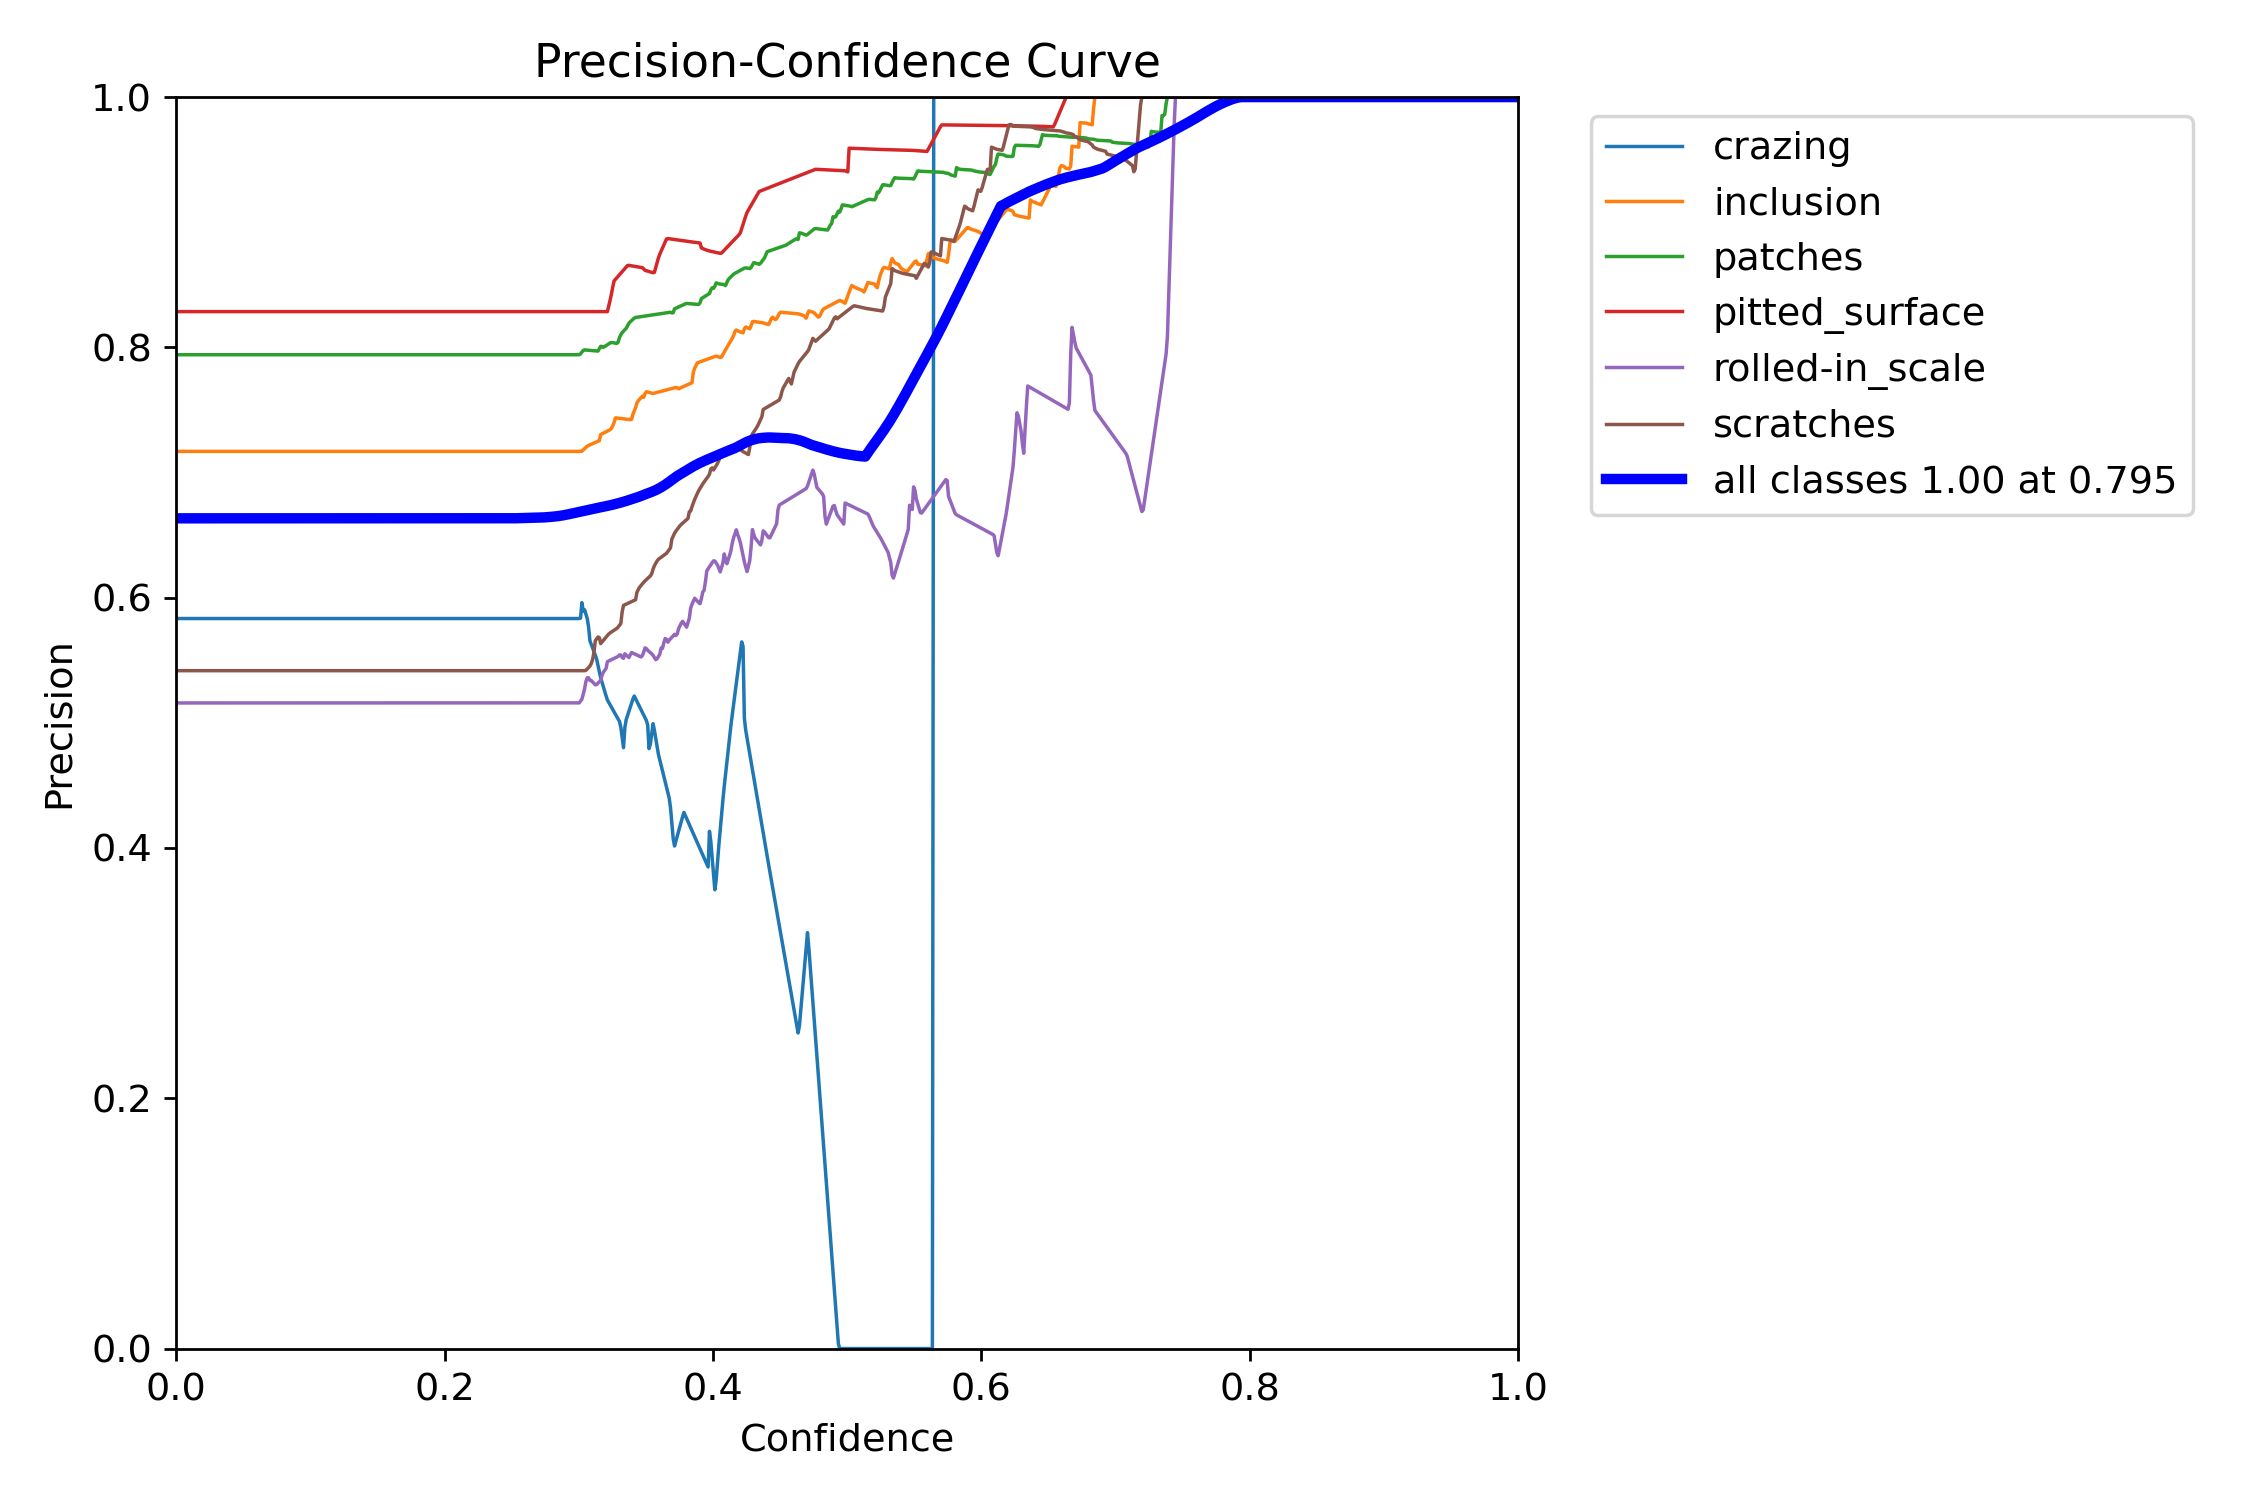
\includegraphics[width=\linewidth]{img/BoxP_curve_soup.png}
			\caption*{(الف) منحنی \lr{Precision-Confidence}}
		\end{minipage}
		\hfill
		\begin{minipage}[b]{0.48\linewidth}
			\centering
			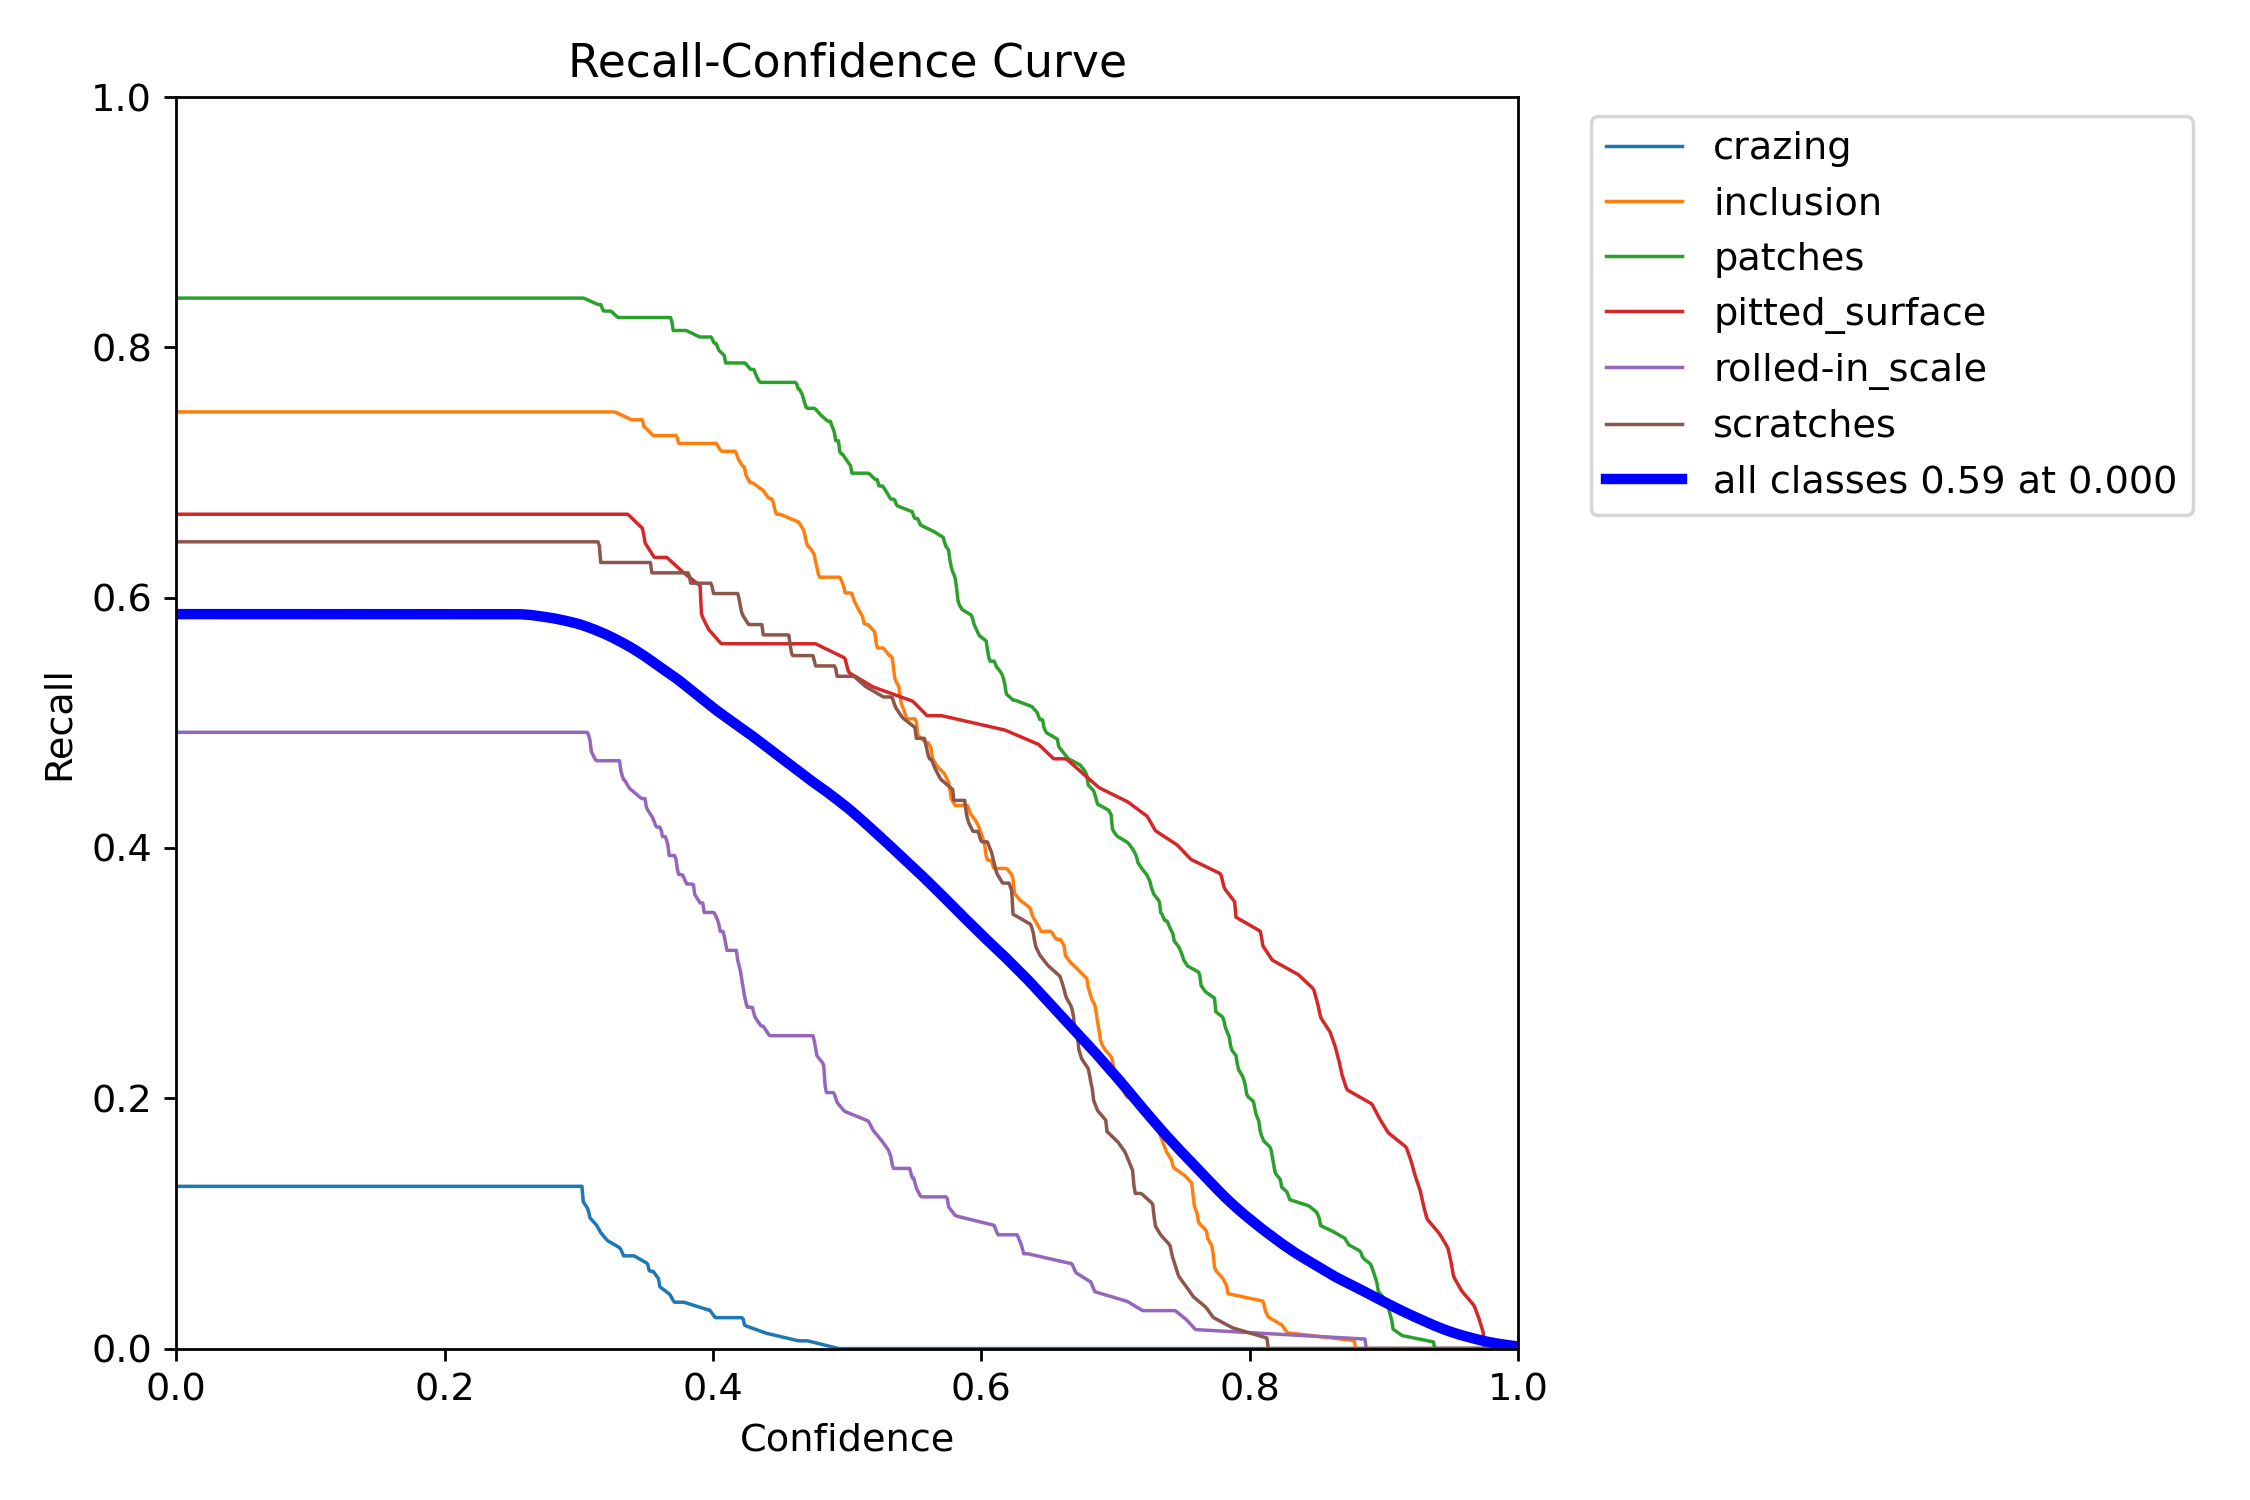
\includegraphics[width=\linewidth]{img/BoxR_curve_soup.png}
			\caption*{(ب) منحنی \lr{Recall-Confidence}}
		\end{minipage}
		
		\vspace{0.35cm}
		
		\begin{minipage}[b]{0.48\linewidth}
			\centering
			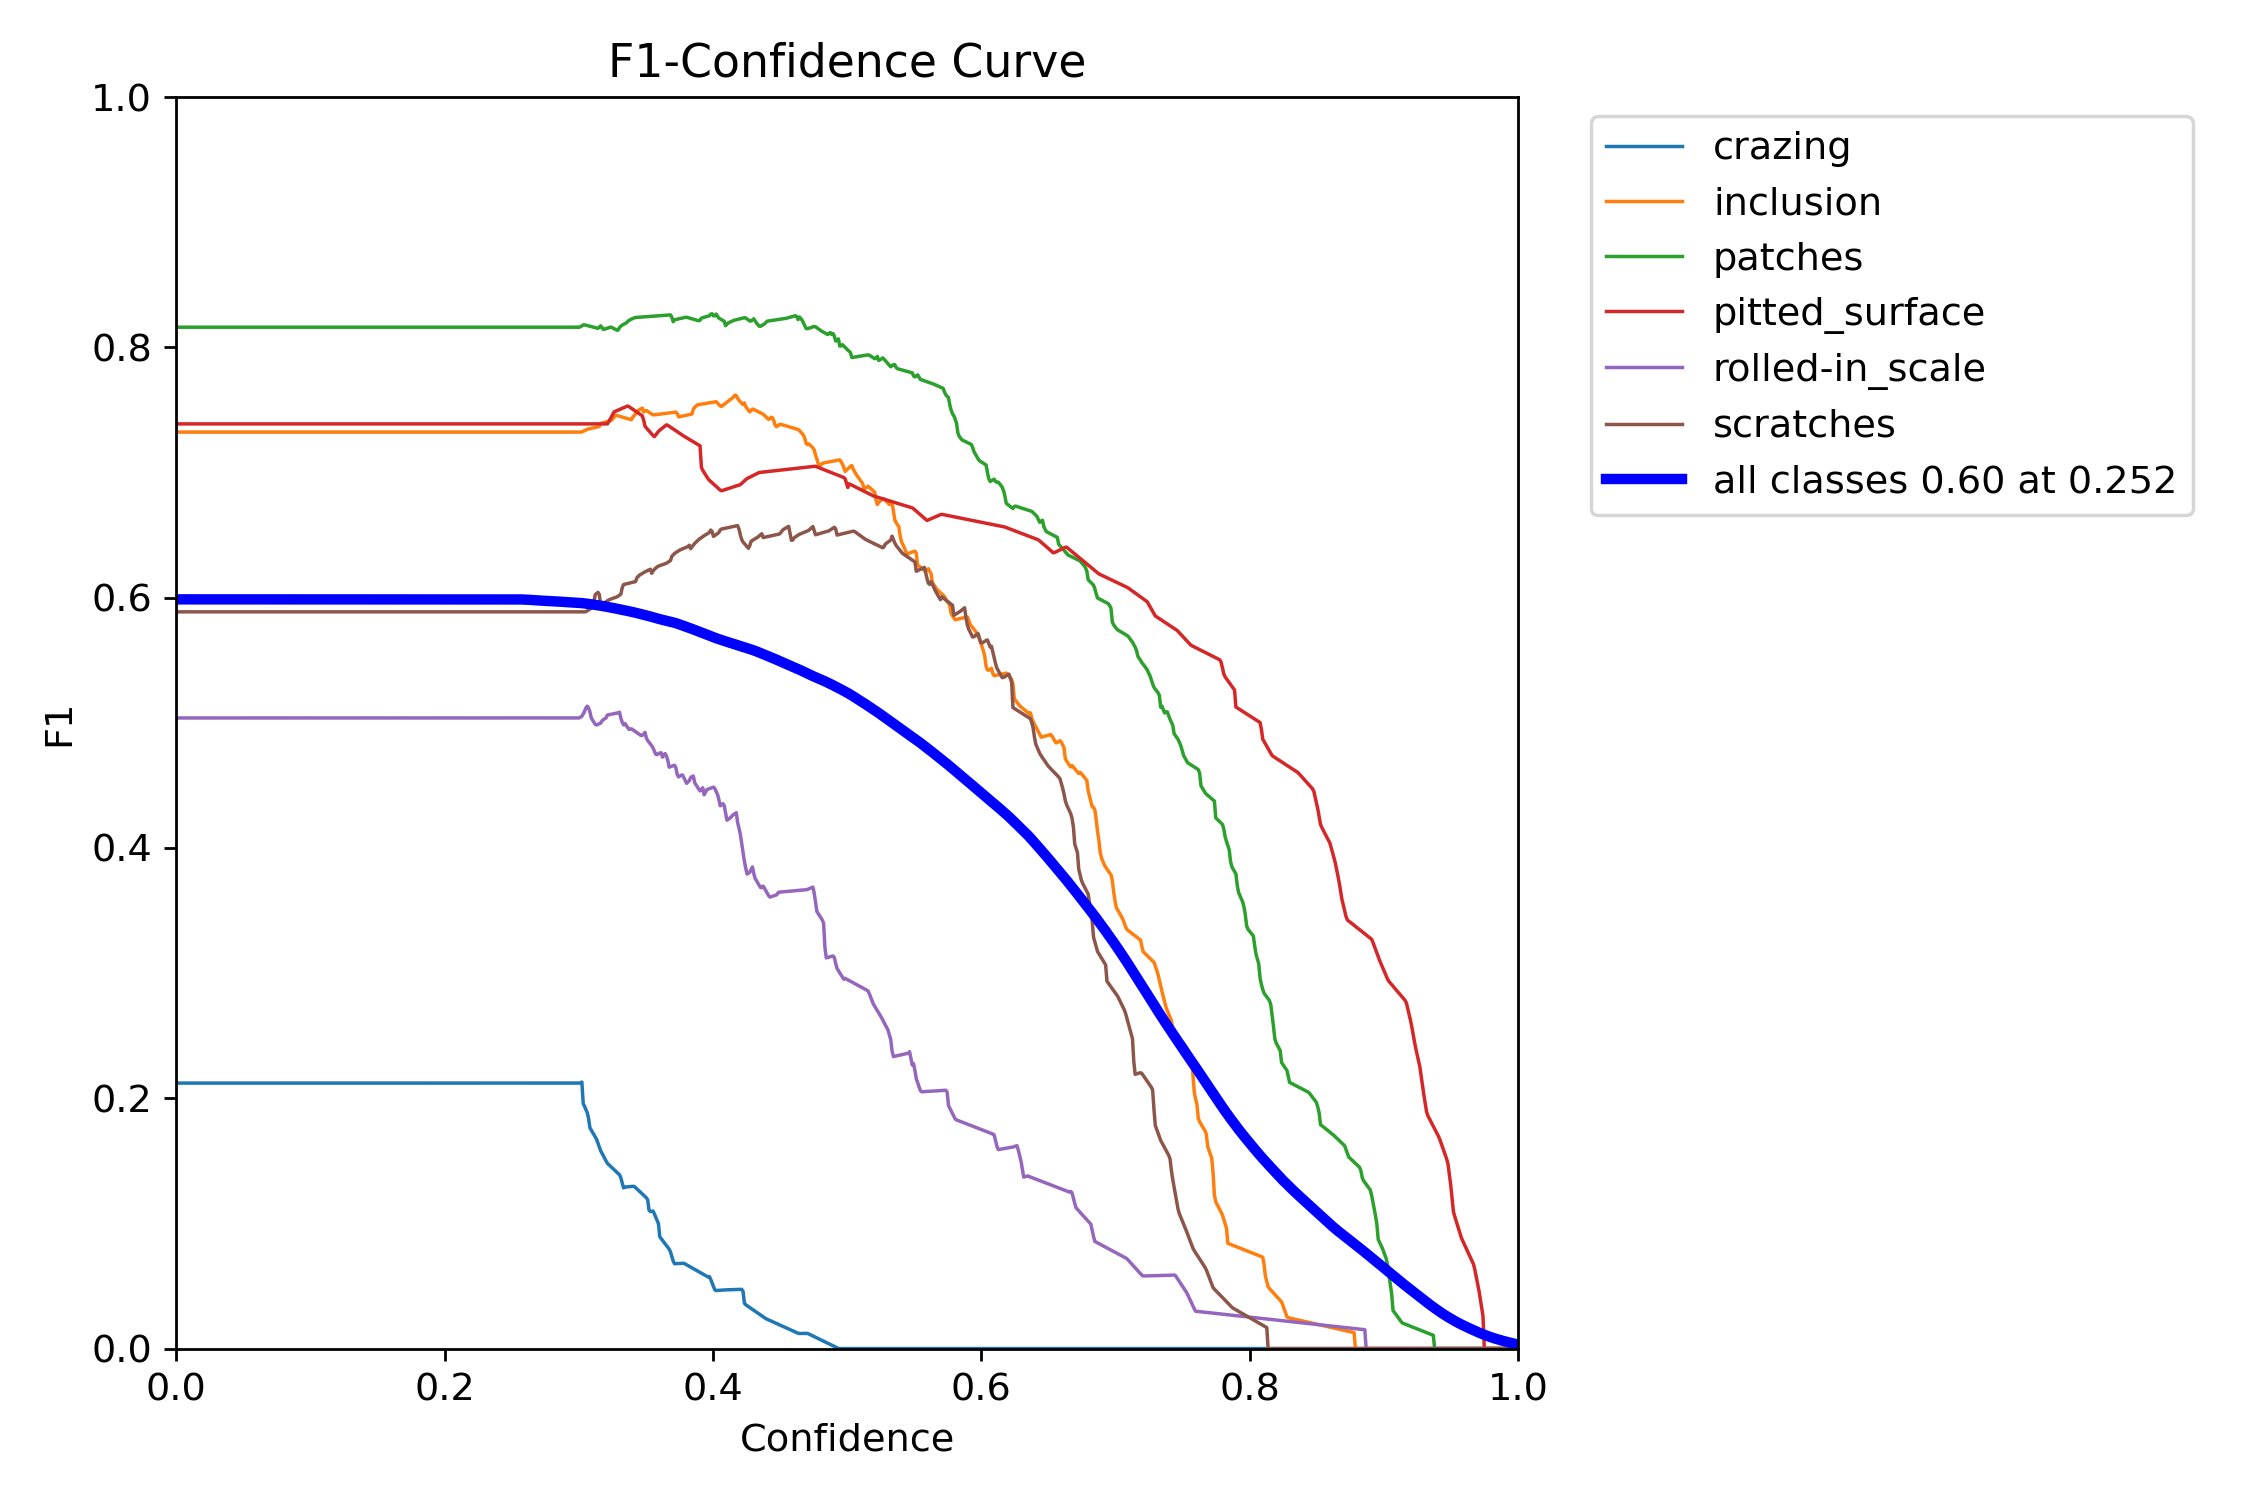
\includegraphics[width=\linewidth]{img/BoxF1_curve_soup.png}
			\caption*{(ج) منحنی \lr{F1-Confidence}}
		\end{minipage}
		\hfill
		\begin{minipage}[b]{0.48\linewidth}
			\centering
			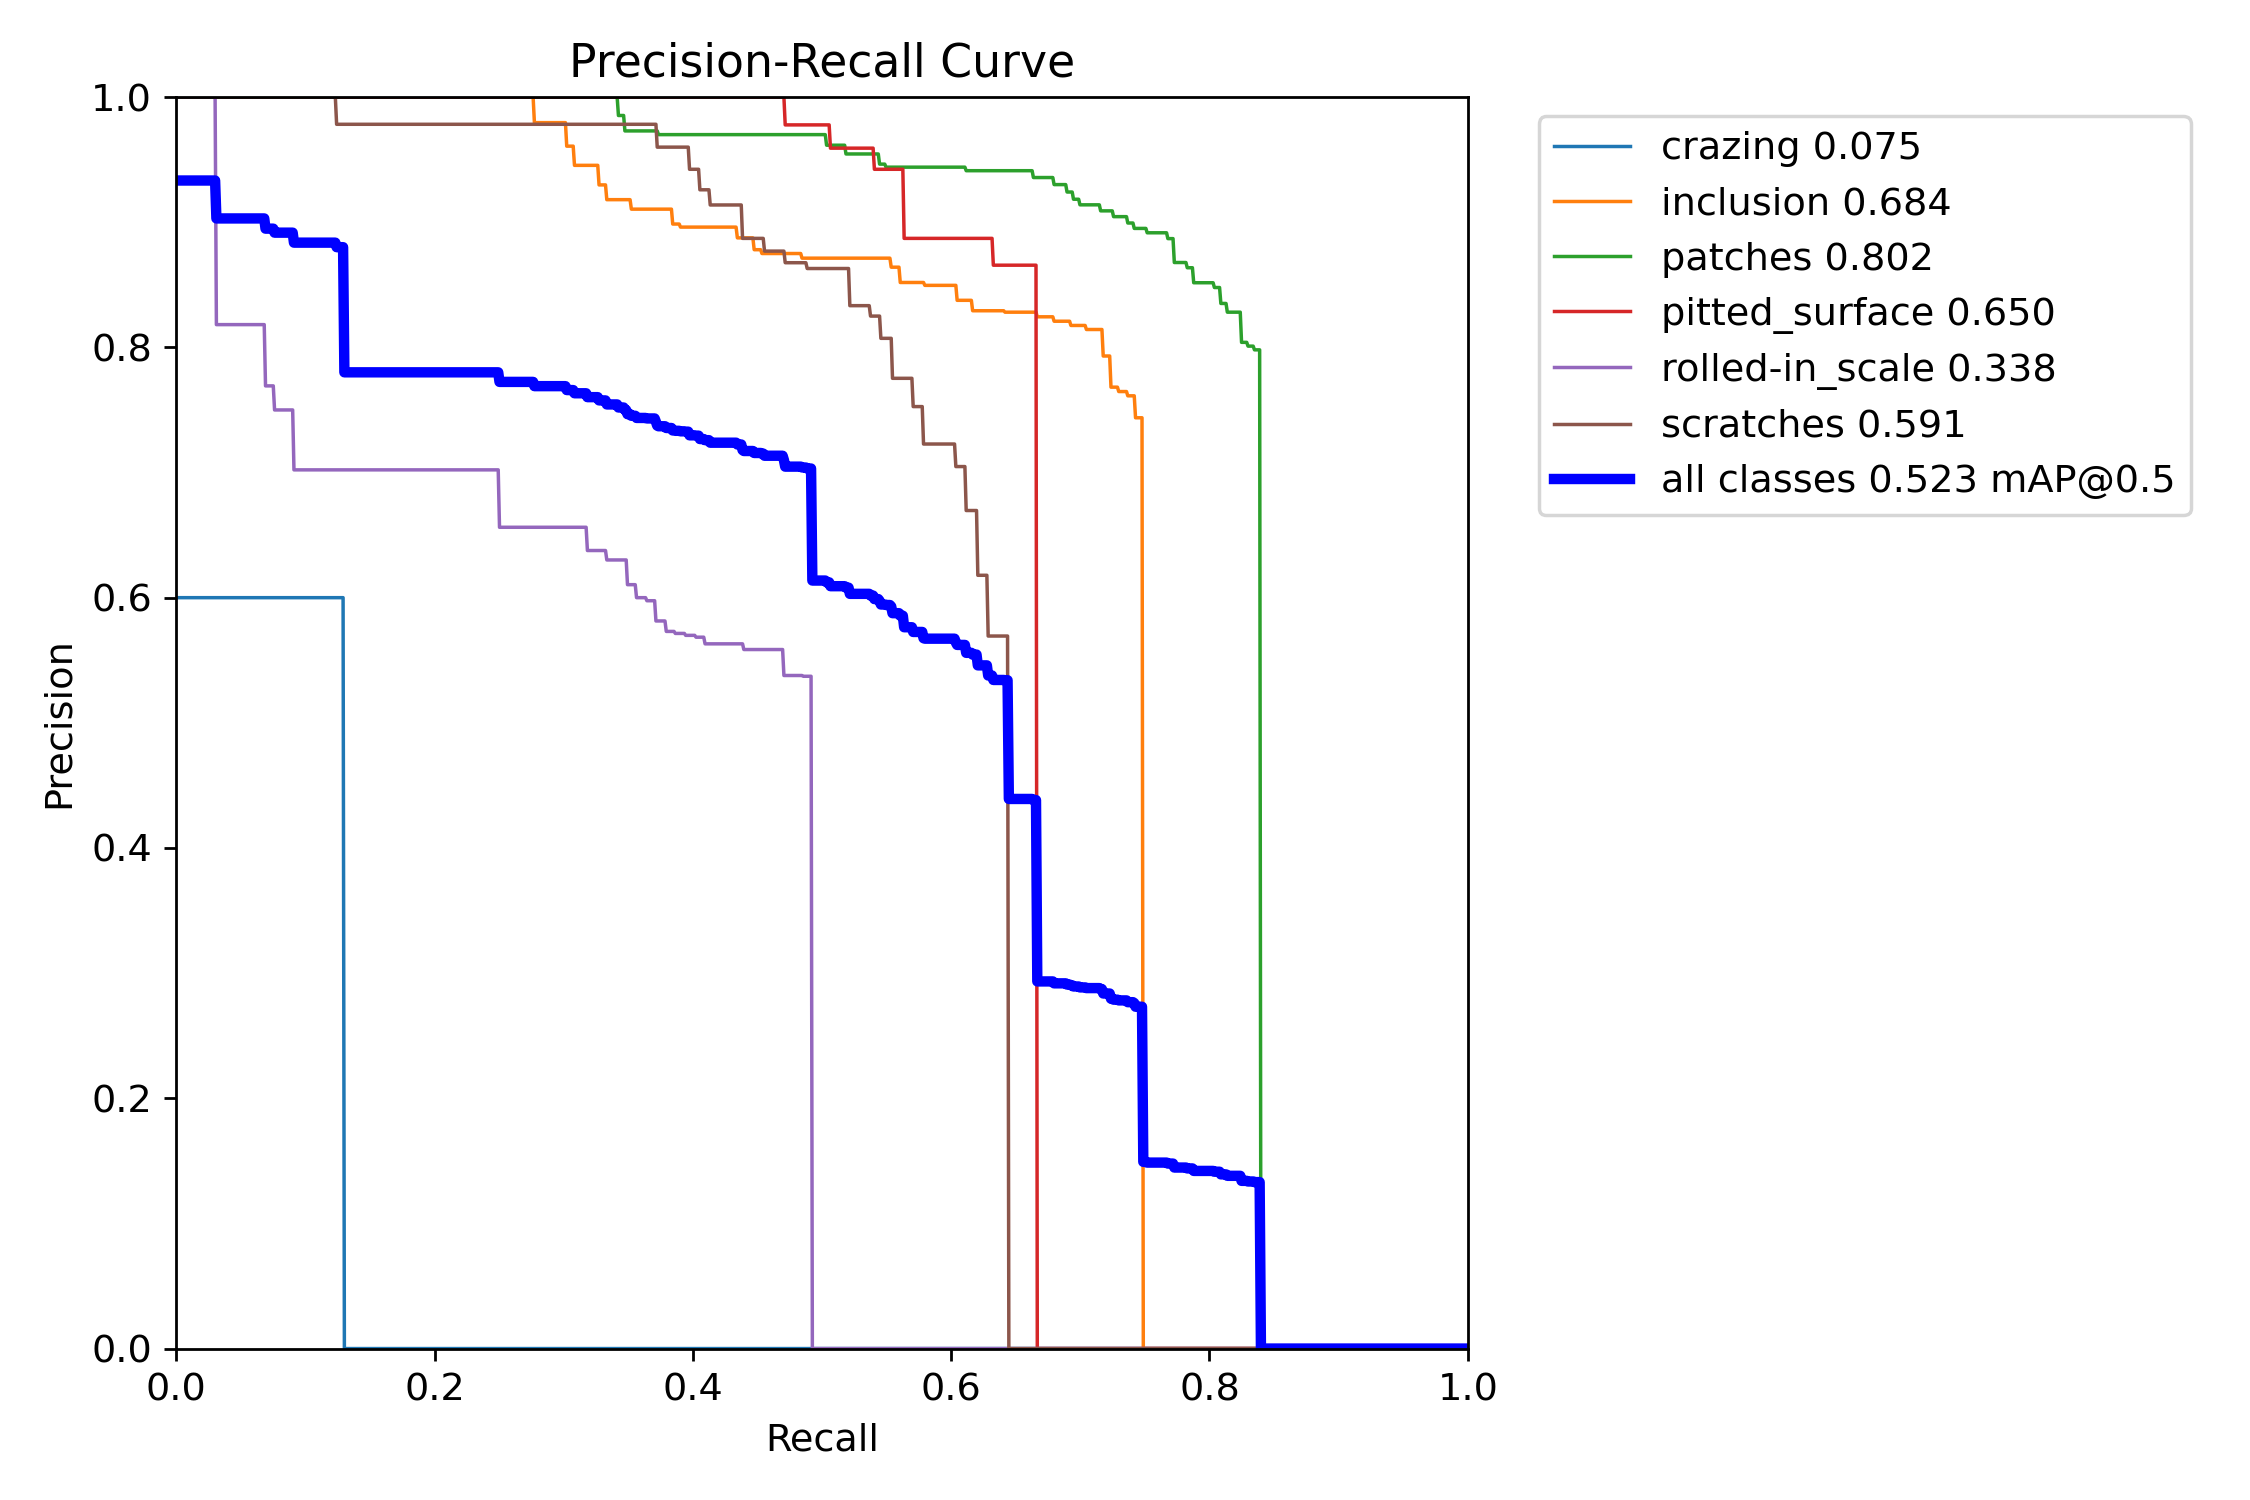
\includegraphics[width=\linewidth]{img/BoxPR_curve_soup.png}
			\caption*{(د) منحنی \lr{Precision-Recall}}
		\end{minipage}
		
		\caption{منحنی‌های ارزیابی عملکرد مدل \lr{Model Soup} روی داده‌های
			اعتبارسنجی.}
		\label{fig:soup-performance-curves}
	\end{figure}
	\newpage
	\subsection{جمع‌بندی نتایج \lr{Model Soup}}
	
	با وجود اینکه ایده \lr{Model Soup} با هدف ترکیب دانش مدل‌های خبره برای
	کلاس‌های مختلف عیب اجرا شد، نتایج نشان دادند که روش پیاده‌سازی‌شده بهبود
	محسوسی نسبت به مدل اصلی \lr{YOLOv8n-Improvement} ایجاد نکرده است. به‌طور
	خاص، مقادیر \lr{mAP@50} و \lr{mAP@50-95} مدل نهایی به سطحی نرسیدند که
	برتری روش میانگین‌گیری مستقیم وزن‌ها را نسبت به مدل پایه اثبات کنند.
	
	یکی از دلایل محتمل این موضوع آن است که میانگین‌گیری ساده همه پارامترها،
	شامل پارامترهای \lr{Backbone}، \lr{Neck} و به‌ویژه \lr{Detection Head}،
	ممکن است بخشی از تخصص یادگرفته‌شده در هر مدل خبره را تضعیف کند. هر مدل
	خبره در طول آموزش به ویژگی‌ها و الگوهای یک کلاس خاص سازگار شده است؛
	بنابراین، میانگین‌گیری مستقیم سرهای آشکارسازی مدل‌ها می‌تواند سبب تداخل
	میان دانش تخصصی کلاس‌های مختلف شود.
	
	در نتیجه، اگرچه آستانه اطمینان \(0.3\) و به‌طور کلی بازه
	\(0.25\) تا \(0.3\) عملکرد متعادل‌تری برای مدل \lr{Model Soup} نشان
	دادند، اما این روش در شکل فعلی خود نتوانست عملکرد \lr{YOLOv8n-Improvement}
	را به‌صورت معنادار بهبود دهد. بنابراین، نتایج این بخش به‌عنوان یک بررسی
	آزمایشی از امکان ترکیب مدل‌های خبره ارائه می‌شوند و از ادعای بهبود قابل
	توجه نسبت به مدل پایه خودداری می‌شود.
	
	
	\subsection{پیشنهادهای توسعه و کارهای آینده}
	
	با توجه به نتایج به‌دست‌آمده، چند مسیر برای بهبود مدل ها پیشنهاد می‌شود:
	
	\begin{itemize}
		
		
		\item ترکیب معماری و سرهای آشکارسازی مدل‌های تک‌کلاسه به‌صورت
		کلاس‌محور؛ به این معنا که به‌جای میانگین‌گیری تمام سرها، برای هر کلاس
		از سر اختصاصی مدل خبره همان کلاس استفاده شود و بخش‌های استخراج ویژگی
		مشترک میان مدل‌ها ترکیب شوند.
		
		\item افزودن یک بلوک یا لایه مبتنی بر تبدیل فوریه سریع (\lr{FFT}) پیش
		از سر آشکارسازی. این لایه می‌تواند ویژگی‌های حوزه فرکانس را استخراج
		کند و در تشخیص بافت‌های ظریف، الگوهای تکرارشونده، ترک‌ها و ساختارهای
		سطحی نامنظم مؤثر باشد.
		
		\item آموزش چند مدل مستقل با مقداردهی اولیه، ترتیب داده یا تنظیمات
		آموزشی متفاوت و استفاده از روش‌های تجمیع خروجی، مانند رأی‌گیری
		(\lr{Voting}) یا \lr{Ensemble Detection}، به‌جای میانگین‌گیری مستقیم
		وزن‌های شبکه‌ها.
	\end{itemize}
	
	این ایده‌ها به دلیل محدودیت زمانی در این پروژه پیاده‌سازی نشدند، اما
	می‌توانند مسیر مناسبی برای توسعه مدل‌های ترکیبی دقیق‌تر و مقاوم‌تر در
	تشخیص عیوب سطحی فولاد باشند.
	
	
	\section{پیاده‌سازی و ارزیابی نسخه پیوسته \lr{PPO}}
	
	پس از پیاده‌سازی نسخه گسسته، نسخه پیوسته‌ی عامل \lr{PPO} نیز روی بهترین
	مدل استخراج عیوب، یعنی \lr{YOLOv8n-Improvement}، اجرا شد. هدف از این
	تغییر، کاهش پرش‌های کنترلی و رسیدن به رفتار نرم‌تر در تنظیم سرعت نوار
	نقاله بود؛ به‌طوری که عامل به‌جای انتخاب یکی از سه عمل گسسته‌ی
	کاهش/حفظ/افزایش سرعت، یک عمل پیوسته در بازه \([-1,1]\) تولید کند و شدت
	تغییر سرعت به‌صورت تدریجی تعیین شود.
	
	\subsection{روند استخراج ویژگی و تعریف حالت}
	
	در هر گام، تصویر ورودی ابتدا با توجه به سرعت فعلی دچار تاری حرکتی
	(\lr{Motion Blur}) می‌شود تا اثر افزایش سرعت بر کیفیت آشکارسازی شبیه‌سازی
	شود. سپس مدل \lr{YOLO} روی تصویر محوشده اجرا می‌شود و چهار ویژگی اصلی
	از خروجی آن استخراج می‌گردد: بیشینه ریسک، میانگین اطمینان،
	تعداد عیوب و فاصله نزدیک‌ترین عیب از مرکز تصویر. ریسک هر عیب بر اساس
	مساحت نرمال‌شده جعبه و ضریب ریسک کلاس محاسبه می‌شود و بیشترین مقدار آن
	به‌عنوان نماینده ریسک کل صحنه به محیط داده می‌شود.
	
	در ادامه، خروجی کنترل‌کننده فازی نیز محاسبه و به بردار حالت افزوده
	می‌شود. بنابراین حالت نهایی شامل شش مؤلفه است:
	ریسک، میانگین اطمینان، سرعت فعلی، تعداد عیوب نرمال‌شده، فاصله نزدیک‌ترین
	عیب از مرکز و خروجی فازی. این ترکیب باعث می‌شود عامل هم اطلاعات بصری
	\lr{YOLO} و هم راهنمایی مبتنی بر دانش خبره را هم‌زمان دریافت کند.
	
	\subsection{تفاوت نسخه پیوسته با نسخه گسسته}
	
	در نسخه گسسته، عامل فقط سه تصمیم مجزا در اختیار داشت و تغییر سرعت به
	اندازه ثابت \(\Delta v\) انجام می‌شد. در نسخه پیوسته، اکشن به یک مقدار
	پیوسته در بازه \([-1,1]\) تبدیل شد و سپس در \(\mathrm{SPEED\_STEP}\)
	ضرب شد. به‌این‌ترتیب، سرعت نهایی به‌صورت تدریجی و با گام‌های نرم‌تری
	تغییر می‌کند.
	
	این تغییر دو اثر مهم دارد. اول اینکه نوسانات ناگهانی سرعت کاهش پیدا
	می‌کند و خروجی کنترلی از حالت پله‌ای به حالت پیوسته‌تر نزدیک می‌شود.
	دوم اینکه عامل می‌تواند شدت واکنش خود را بهتر تنظیم کند؛ یعنی در برابر
	ریسک‌های متوسط، الزاماً به حداکثر کاهش یا افزایش سرعت متوسل نمی‌شود و
	می‌تواند تغییرات کوچک‌تری اعمال کند. همین موضوع باعث شد رفتار کنترل در
	نمودار ارزیابی، نرم‌تر از نسخه گسسته دیده شود.
	
	\paragraph{دلیل نرم‌تر شدن رفتار}
	
	نرم‌تر شدن پاسخ کنترلی در نسخه پیوسته از سه منبع اصلی می‌آید:
	\begin{itemize}
		\item فضای عمل پیوسته، که اجازه می‌دهد خروجی سیاست به‌جای تصمیم‌های
		دوحالته یا سه‌حالته، هر مقدار میانی را نیز تولید کند.
		\item جریمه نرمی تغییر سرعت، که عامل را از جهش‌های شدید بازمی‌دارد.
		\item بهینه‌سازی بازده تجمعی در \lr{PPO}، که باعث می‌شود سیاست به
		سمت پاسخ‌های پایدارتر و کم‌نوسان‌تر حرکت کند.
	\end{itemize}
	
	\subsection{تابع پاداش و نقش فازی}
	
	تابع پاداش در نسخه پیوسته همچنان ترکیبی از چند مؤلفه است: هم‌راستایی با
	فازی، قوانین نرم مبتنی بر ریسک، پاداش اطمینان، پاداش/جریمه مبتنی بر
	سرعت و ریسک، و جریمه تغییرات ناگهانی سرعت. با این حال، چون اکشن اکنون
	پیوسته است، سیاست عامل می‌تواند بخشی از این منطق را خودش یاد بگیرد و
	نیاز آن به پیروی مستقیم از خروجی فازی کمتر شود.
	
	به همین دلیل، نسبت به نسخه گسسته، وابستگی کامل به فازی کاهش یافته و
	عامل سهم بیشتری در تعیین رفتار نهایی پیدا کرده است. این تغییر از یک طرف
	باعث افزایش انعطاف سیاست و تولید کنترل نرم‌تر شده، اما از طرف دیگر
	می‌تواند بخشی از مزیت نسخه گسسته را که بیشتر به ساختار فازی متکی بود،
	کاهش دهد. بنابراین مشاهده می‌شود که هرچند رفتار کنترلی نرم‌تر شده، اما
	عملکرد کلی لزوماً به همان اندازه نسخه گسسته بهبود پیدا نکرده است.
	
	\subsection{آموزش عامل \lr{PPO}}
	
	آموزش با \lr{Stable-Baselines3} و سیاست \lr{MlpPolicy} انجام شد.
	شبکه سیاست از لایه‌های \([64,64]\) و شبکه ارزش از لایه‌های \([128,128]\)
	استفاده می‌کند. نرخ یادگیری \(10^{-4}\)، طول هر rollout برابر با
	\(1024\)، اندازه دسته \(64\)، تعداد epochهای به‌روزرسانی \(8\)،
	\(\gamma=0.985\)، \(\lambda=0.95\) و ضریب برش \(0.15\) برای آموزش
	در نظر گرفته شد. همچنین ضریب آنتروپی \(0.10\) و ضریب تابع ارزش \(0.6\)
	برای متعادل‌سازی اکتشاف و پایداری گرادیان‌ها استفاده شد.
	
	برای پایش کیفیت آموزش، یک callback ارزیابی دستی تعریف شد که در هر
	\(EVAL\_FREQ\) گام، عامل را روی مجموعه اعتبارسنجی اجرا می‌کند و
	میانگین پاداش چند اپیزود را ثبت می‌نماید. هر زمان که میانگین پاداش
	بهتر از مقدار قبلی می‌شد، مدل به‌عنوان بهترین نسخه ذخیره می‌گردید.
	این روند باعث شد انتخاب مدل نهایی بر مبنای عملکرد واقعی در محیط
	اعتبارسنجی انجام شود، نه صرفاً مقدار loss آموزشی.
	
	\subsection{تحلیل نمودار عملکرد نسخه پیوسته}
	
	شکل زیر روند تغییر سرعت نوار نقاله و ریسک عیب را در طول زمان نشان می‌دهد.
	در بخش‌هایی از نمودار، سرعت با شیب ملایم‌تری تغییر کرده و از جهش‌های
	شدید نسخه گسسته فاصله گرفته است. این رفتار نشان می‌دهد که عامل پیوسته
	توانسته است به‌جای تصمیم‌های ناگهانی، کنترل نرم‌تری اعمال کند.
	
	\begin{figure}[htbp]
		\centering
		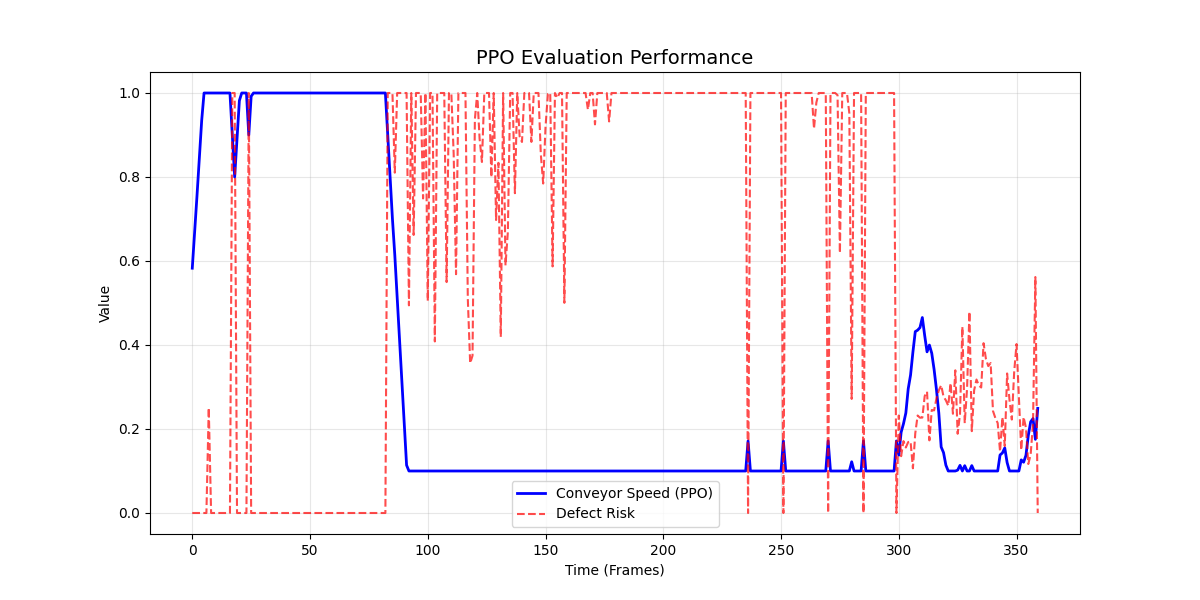
\includegraphics[width=0.92\linewidth]{img/ppo_performance_plot_contineu.png}
		\caption{ارزیابی عملکرد نسخه پیوسته \lr{PPO} روی مدل
			\lr{YOLOv8n-Improvement}. منحنی آبی تغییرات سرعت نوار نقاله و منحنی
			قرمز تغییرات ریسک عیب را در طول زمان نشان می‌دهد.}
		\label{fig:ppo-continuous-performance}
	\end{figure}
	
	در این نمودار مشاهده می‌شود که سرعت در برخی بازه‌ها به‌صورت تدریجی کاهش
	یافته و سپس در نواحی کم‌ریسک دوباره افزایش پیدا کرده است. این نوع
	رفتار، نسبت به نسخه گسسته، واقعی‌تر و نرم‌تر است؛ زیرا تغییر سرعت
	بر اساس میزان ریسک و نه صرفاً یک تصمیم جهشی انجام می‌شود. با این حال،
	در برخی بازه‌ها، کاهش محسوس عملکرد نیز دیده می‌شود. علت اصلی این موضوع
	آن است که عامل در نسخه پیوسته آزادی بیشتری برای دور شدن از راهنمای فازی
	پیدا کرده و همین امر موجب شده بخشی از مزیت نسخه گسسته که به‌طور
	مستقیم‌تر به فازی متکی بود، کاهش یابد.
	
	\subsection{جمع‌بندی}
	
	در مجموع، نسخه پیوسته \lr{PPO} روی \lr{YOLOv8n-Improvement} توانست
	رفتار کنترلی نرم‌تر و پیوسته‌تری نسبت به نسخه گسسته ایجاد کند و از
	جهش‌های ناگهانی سرعت بکاهد. با این حال، این نرمی بیشتر با افت نسبی
	عملکرد همراه شد؛ یعنی مدل، در عوضِ پایبندی بیشتر به ساختار فازی،
	بیشتر به سیاست یادگرفته‌شده توسط خود عامل اتکا کرد. بنابراین، نسخه
	پیوسته از نظر کیفیت حرکت و نرمی کنترل مزیت دارد، اما نسخه گسسته در
	برخی سناریوها هنوز از نظر کارایی نهایی و وابستگی بهتر به دانش فازی
	نتیجه بهتری ارائه می‌دهد.
	
	
	
	\section{شبیه‌سازی}
	در پروژه اصلی، برای سنجش عملکرد مدل و شبیه سازی حرکت ورقه های فولادی بر روی نوار نقاله، عکس های تست ورقه های فولادی در قالب یک ویدیو ذخیره و به مدل داده شد. مدل به ترتیب تصاویر درون ویدیو را خوانده، عیوب ورقه را نشخیص داده و سرعت را تغییر می‌دهد. تغییر سرعت در این ویدیو با میزان تاری ناشی از حرکت ورقه و نمایش عدد سرعتی که کنترلر rl تعیین می‌کند شبیه سازی می‌شود.\\
	
	اما برای شبیه سازی دقیق و نزدیک شدن به محیط واقعی، نیاز بود که به جای استفاده از ویدیو، محیط شبیه سازی‌ای ایجاد شود تا به طور دقیق حرکت ورقه ها روی نوار نقاله، تصویربرداری از ورقه ها توسط یک دوربین، تشخیص عیوب  و تنظیم سرعت حرکت ورقه های فولادی را شبیه سازی کند. برای رسیدن به این هدف، در این بخش عملکرد مدل ساخته شده در محیط webot شبیه سازی می‌شود.\\
	
	برای مصالحه بین سرعت و دقت شبیه سازی، از بین 3 معماری YOLO پیاده سازی شده در پروژه، از \lr{YOLOV8 Improvement}استفاده شده است. همچنین برای کنترل سرعت ورقه ها، از هر 2 معماری Q-Learning و PPO استفاده شده است. در نهایت با نوشتن کد کنترلر و استفاده از وزن های آموزش دیده YOLO، PPO و Q-Learning، ارتباط بین اجزای شبیه سازی برقرار شده و هر بخش وظیفه خود را انجام میدهد
	\subsection{شماتیک کلی و اجزای شبیه سازی}
	\begin{figure}[H]
		\centering
		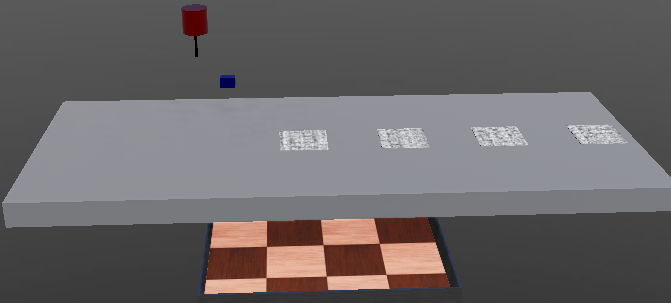
\includegraphics[width=0.8\linewidth]{img/shematic} 
		\caption{شماتیک کلی و اجزای شبیه‌سازی در محیط Webots}
		\label{fig:shematic}
	\end{figure}
	شکل 1 شماتیک کلی محیط شبیه سازی را نشان می‌دهد. اجزای این شبیه سازی شامل یک نوار نقاله به شکل مکعب مستطیل، یک دوربین (به رنگ آبی)، یک ربات علامت گذار با یک درجه آزادی (در بخش های بعدی توضیح داده خواهد شد) و 4 ورقه فولادی می‌باشد.
	\begin{itemize}
		\item نوار نقاله: با استفاده از یک solid محیط webot ساخته شده است. برای نمایش این solid، یک shape به صورت مکعب مستطیل به طول \lr{2.5}، عرض 1 و ارتفاع \lr{0.1} استفاده شده است. برای جلوگیری از تشخیص های اشتباه yolo، رنگ این نوار به سفید تغییر یافته است
		\item ورقه های فولادی: برای اینکه بتوانیم تصاویر فولاد های معیوب را روی نوار نقاله قرار دهیم، نیاز داریم که این تصاویر بر روی یک شی webot قرار بگیرند. در نتیجه 4 شی solid با shape های مکعب مستطیلی به طول \lr{0.2}، عرض \lr{0.2} و ارتفاع \lr{0.01} تعریف شده‌اند. با تعریف بخش appearance این ورقه هااز نوع ImageTexture، قادر خواهیم بود که با دادن آدرس پوشه تصاویر، آن ها را بر روی این ورقه های فولادی قرار دهیم. در هر لحظه 4 تصویر از پوشه تصاویر تست بر روی این 4 ورقه قرار می‌گیرند.  انتخاب 4 ورقه باعث پیوستگی حرکت ورقه های فولادی شده و شبیه سازی را به محیط های واقعی نزدیک تر می‌کند.با عبور هر ورقه از زیر دوربین و ربات علامت‌گذار، ورقه به اول نوار نقاله بازگشته و تصویر بعدی روی آن قرار میگیرد. همچنین تلاش شده است که فاصله بین این 4 ورقه یکسان و به اندازه ابعاد ورقه ها باشد. ایجاد این فاصله تضمین میکند که چندین ورقه به طور همزمان در زیر دوربین قرار نگرفته و همچنین بعد از عبور ورقه معیوب از زیر دوربین، فرصتی برای افزایش سرعت نوار و شبیه سازی دقیق تر به وجود بیاید.
		\item دوربین و ربات علامت‌گذار: چون این دو سنسور و عملگر یک موجودیت برنامه‌پذیر هستند و با کد کنترلر کنترل میشوند، در قالب children های گره Robot تعریف میشوند. گره دوربین در قالب زیرمجموعه این ربات تعریف شده و وظیفه آن، تصویربرداری از نوار نقاله و ارسال آن به مدل YOLO برای تشخیص عیب و تنظیم سرعت است. چون ابعاد تصاویر ما $200\times200$ هستند، و محیط webot برای رندر گرافیکی، ابعاد تصاویر را به $256\times256$ تغییر می‌دهد، رزولوشن دوربین نیز $256\times256$ تعریف شده است. تا تشخیص YOLO دچار مشکل نشود.
		
		برای شبیه سازی بازوی علامت‌گذار نیز از یک sliderjoint استوانه ای که فقط در محور y حرکت می‌کند و یک قلم علامت‌گذار pen که زیرمجموعه این بازو می‌باشد استفاده شده است
		
		برای پیاده‌سازی مکانیزم تغذیه پیوسته تصاویر روی نوار نقاله، نود رباتِ بازرس در حالت Supervisor پیکربندی شد. این سطح از دسترسی به کنترلر اجازه داد تا به صورت پویا تکسچر ورقه‌های فلزی را به‌روزرسانی کرده و مختصات آن‌ها را برای ایجاد یک لوپ بی‌نهایت و پیوسته تنظیم نماید.
		
		
		\begin{figure}[H]
			\centering
			\begin{subfigure}[b]{0.45\linewidth}
				\centering
				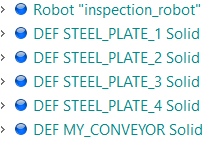
\includegraphics[width=\linewidth]{img/main nodes}
				\caption{گره‌های اصلی محیط شبیه‌سازی شامل نوار نقاله و ورقه‌های  فولادی و ربات بازرس}
				\label{fig:nodes_main}
			\end{subfigure}
			\hfill
			\begin{subfigure}[b]{0.45\linewidth}
				\centering
				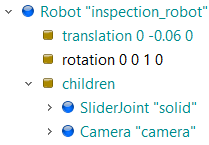
\includegraphics[width=\linewidth]{img/Robot nodes}
				\caption{زیرمجموعه‌های گره ربات بازرس شامل دوربین و مفاصل حرکتی}
				\label{fig:nodes_robot}
			\end{subfigure}
			
			\caption{نمایش ساختار درختی  و معماری گره‌ها در نرم‌افزار Webots}
			\label{fig:webots_scene_tree}
		\end{figure}
	\end{itemize}
	\subsection{چرخه عملکرد شبیه‌سازی}
	
	ساختار شبیه‌سازی در این پروژه به گونه‌ای طراحی شده است که فرآیند بازرسی پیوسته صنعتی را در قالب یک حلقه تکرارشونده با بالاترین بهره‌وری محاسباتی اجرا کند. این چرخه از فاز مقداردهی اولیه آغاز شده و سپس در هر گام زمانی شبیه‌ساز، مجموعه‌ای از عملیات سینماتیکی، پردازش تصویر و تصمیم‌گیری هوشمند را به ترتیب زیر به انجام می‌رساند:
	
	\begin{enumerate}
		\item \textbf{فاز مقداردهی اولیه:}
		پیش از ورود به حلقه اصلی، ابتدا مدل‌های هوش مصنوعی (مدل تشخیص عیوب\lr{ YOLOv8} و مدل کنترل‌کننده \lr{PPO/Q-Learning}) در حافظه بارگذاری می‌شوند. سپس ارتباط با گره‌های (Nodes) محیط Webots از جمله دوربین بازرسی و ورقه‌های فولادی برقرار شده و 4 تصویر ابتدایی از دیتاست تست، به عنوان بافت (Texture) روی 4 ورقه ‌فولادی اعمال می‌گردد.
		
		\item \textbf{به‌روزرسانی سینماتیکی و ایجاد چرخه بی‌نهایت:}
		در آغاز هر گام زمانی، مختصات فضایی ورقه‌های فولادی بر اساس سرعت فعلی نوار نقاله در راستای محور حرکت \lr{x} به‌روزرسانی می‌شود. برای جلوگیری از نیاز به تولید تعداد نامحدود شی فیزیکی در شبیه‌ساز، یک مکانیزم بازیافت (Recycling) طراحی شده است؛ به این صورت که اگر ورقه‌ای از میدان دید دوربین خارج شده و از مرز تعیین‌شده (\lr{END\_X}) عبور کند، به طور خودکار به اندازه طول مشخصی به عقب منتقل می‌شود و بافت آن با تصویر جدیدی از دیتاست جایگزین می‌گردد. این تکنیک، حرکت پیوسته و بی‌نهایتِ خط تولید را شبیه‌سازی می‌کند.
		
		\item \textbf{ادراک بینایی و پیش‌پردازش تصویر:}
		پس از حرکت ورقه‌ها، سنسور دوربین یک فریم از وضعیت فعلی محیط ثبت می‌کند. این فریم خام پس از استخراج و اعمال الگوریتم بهبود کنتراست (\lr{CLAHE} در فضای \lr{Grayscale}) آماده‌سازی می‌شود تا شرایط نوری آن دقیقاً با شرایط تصاویر زمان آموزش مدل یکسان شود.
		
		\item \textbf{پردازش توسط بینایی ماشین (\lr{YOLOv8}):}
		فریم پیش‌پردازش‌شده به عنوان ورودی به مدل YOLO داده می‌شود. خروجی این مرحله شامل مختصات جعبه‌های محصورکننده (\lr{Bounding Boxes})، کلاس عیوب و میزان اطمینان (Confidence) شبکه است. بر اساس مساحت عیوب و ضریب ریسک هر کلاس، یک امتیاز ریسک وزنی استخراج می‌گردد.
		
		\item \textbf{تصمیم‌گیری ترکیبی (\lr{Fuzzy-DRL}):}
		اطلاعات استخراج‌شده (شامل ریسک، سرعت فعلی، میانگین اطمینان، تعداد عیوب و فاصله آن‌ها تا مرکز تصویر) به عنوان وضعیت سیستم (\lr{State}) تجمیع می‌شوند. ابتدا سیستم منطق فازی یک پیشنهاد اولیه برای تغییر سرعت ارائه می‌دهد؛ سپس شبکه عصبی PPO (یا عامل \lr{Q-Learning}) با بررسی جامع وضعیت، عمل  نهایی را برای ترمز، شتاب یا حفظ سرعت صادر می‌کند.
		
		\item \textbf{اعمال فرمان و نظارت:}
		در گام نهایی، تغییرات محاسبه‌شده به سرعت فعلی سیستم اعمال می‌شود (با رعایت محدودیت‌های حداقل و حداکثر سرعت مجاز). سپس داشبورد مانیتورینگ سیستم، فریم حاشیه‌نویسی‌شده را به همراه پارامترهای بلادرنگ سرعت و ریسک در یک پنجره گرافیکی نمایش می‌دهد و شبیه‌ساز برای اجرای گام زمانی بعدی آماده می‌شود.
		
		\begin{figure}[H]
			\centering
			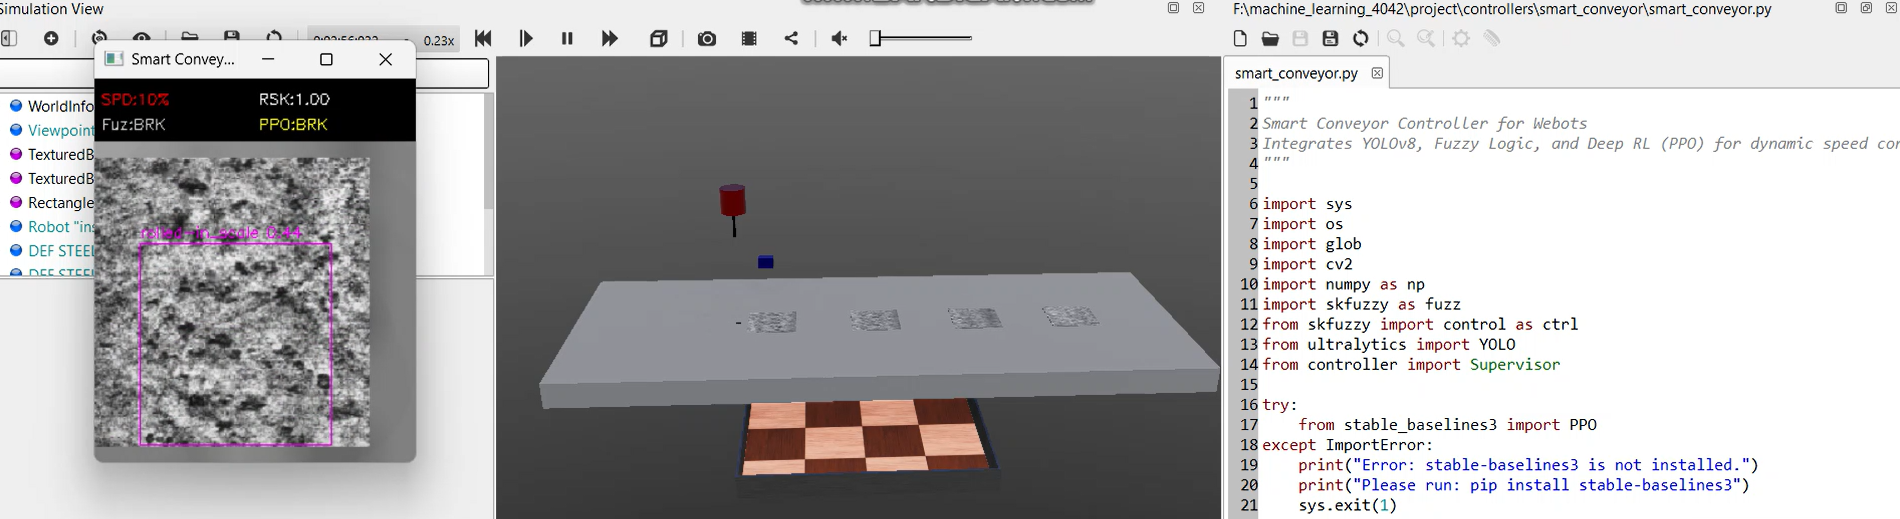
\includegraphics[width=\linewidth]{img/simulation output}
			\caption{نمای کلی اجرای شبیه‌سازی در محیط \lr{Webots}؛ شامل محیط سه‌بعدی نوار نقاله (وسط)، کد کنترلر (راست) و داشبورد مانیتورینگ بلادرنگ (چپ) که تشخیص عیوب و تصمیمات ترکیبی \lr{PPO} و منطق فازی را نمایش می‌دهد.}
			\label{fig:simulation_output}
		\end{figure}
	\end{enumerate}
	
	\subsection{مشکلات به وجود آمده در فرایند شبیه سازی و حل آنها}
	\begin{enumerate}
		\item \textbf{زاویه اشتباه دریافت تصاویر: }این مهم ترین مشکل به وجود آمده در فرایند شبیه‌سازی بود. در شبیه‌سازی، تصاویر به ترتیب روی ورقه ها قرار گرفته و در جهت محور $x$ حرکت می‌کردند اما به دلیل اینکه دوربین نیز در جهت محور $x$ قرار گرفته بود، دوربین تصاویر را با 90 درجه چرخش دریافت و به YOLO تحویل میداد. از آنجایی که شبکه های YOLO به چرخش حساس هستند(مگر اینکه عکس های چرخیده شده نیز آموزش دیده شده باشند) تشخیص عیوبی که در یک جهت کشیده شده‌اند، مانند \lr{crazing, inclusion} و \lr{rolled in scale} با مشکل مواجه میشد. برای حل این مشکل، با چرخش 90 درجه ای تصاویر در جهت ساعتگرد، قبل از اینکه وارد YOLO شوند، دقت مدل بسیار افزایش یافت
		\item \textbf{دستکاری معماری \lr{YOLO}:} بخشی از لایه هایی که در فرایند آموزش برای بهبود توجه و عملکرد YOLO استفاده و با استفاده از آنها وزن های آموزش دیده مدل تولید شده بود، مانند \lr{GSEBlock Improvement} به اشتباه در مسیر forward استنتاج YOLO در محیط شبیه سازی قرار گرفته بودند. در نتیجه PyTorch در مواجهه با یک لایه جدید، وزن های تصادفی تولید میکرد. در واقع وزن های آموزش دیده با موفقیت لود می‌شدند. اما در مواجهه با لایه های جدید در مسیر forward، وزن های این لایه به صورت تصادفی مقداردهی می‌شدند که مقداری از دقت مدل را کاهش میداد.
		\item \textbf{عدم استفاده از الگوریتم \lr{CLAHE}:} یکی از الگوریتم های پیش پردازش در فرایند آموزش، بهبود کنتراست تصاویر با استفاده از الگوریتم CLAHE برای برجسته تر کردن عیوب بود. در فرایند شبیه سازی نیز این الگوریتم بر فریم های دریافت شده از دوربین قبل از اینکه وارد YOLO بشوند، اعمال می‌شود. عدم استفاده از این الگوریتم باعث کاهش دقت در کلاس های Crazing  شد
		\item \textbf{ارتفاع دوربین:} فرایند آموزش با استفاده از تصاویر $200\times200$ ورقه‌های فولادی خراب انجام شد. اما در محیط شبیه‌سازی، فریمی که در نهایت به \lr{YOLO} داده می‌شود، تصویری است که دوربین از محیط شبیه‌سازی دریافت می‌کند. افزایش ارتفاع دوربین باعث می‌شد ورقه فولادی بخش کوچکی از فریم دریافت شده باشد و کاهش ارتفاع دوربین باعث می‌شد که دوربین فقط بخشی از ورقه فولادی را دریافت کند. هر دو اتفاق باعث کاهش دقت مدل و عدم تشخیص بخشی از عیوب می‌شد. در نتیجه، ارتفاع دوربین باید به اندازه‌ای باشد که زمانی که ورقه فولادی به طور کامل در زیر دوربین قرار می‌گیرد، ابعاد ورقه دقیقاً تمام کادر تصویر را پر کند (لبه‌به‌لبه شود)  تا بیشترین تطابق ممکن را با شرایط تصاویر دیتاست آموزشی داشته باشد.
		\item \textbf{استفاده از نوار نقاله آماده \lr{webot}:} در ابتدا از یک نوار نقاله آماده استفاده و سرعت لحظه ای سیستم به موتور نوار نقاله داده می‌شد. اما رنگ سیاه نوار نقاله و ظاهر برجسته آن باعث تشخیص های اشتباه و ناخواسته در مرز بین ورقه ها و نوار نقاله می‌شد. به جای استفاده از نوار نقاله آماده که ظاهر آن غیرقابل تغییر دادن بود، از یک solid به عنوان نوار نقاله استفاده و رنگ آن به سفید تغییر داده شد. سرعت لحظه ای سیستم نیز به جای اینکه بر موتور نوار نقاله اعمال شود، بر خود ورقه ها اعمال شده و با استفاده از روابط سینماتیک، مختصات ورقه ها در جهت محور $x$ تغییر می‌کند. 
		\item \textbf{اضافه کردن لامپ:} در محیط شبیه سازی از روشنایی لامپ استفاده شد اما بازتاب های نوری شدید لامپ از سطح ورقه های فولادی باعث خراب شدن تصاویر ورقه ها می‌شد و از محیط شبیه سازی حذف شد
	\end{enumerate}
	
	در حال حاضر تمامی مشکلات به وجود آمده در محیط شبیه سازی برطرف شده و چرخه تشخیص و کنترل سرعت با موفقیت انجام می‌شود. اما اعمال الگوریتم \lr{CLAHE} علی‌رغم افزایش دقت مدل در تشخیص عیوب \lr{Crazing}، باعث تشخیص های اشتباه pitted surface در برخی از کلاس عیوب می‌شود. با کاهش شدت کنتراست از \lr{2.5} به \lr{1.5}، مصالحه ای در دقت مدل به دست آمده است اما تشخیص های اشتباه کمی همچنان وجود دارند.
	
	\subsection{نتایج شبیه سازی}
	
	\begin{figure}[H]
		\centering
		
		\begin{subfigure}[b]{0.42\linewidth}
			\centering
			
\includegraphics[width=\linewidth]{img/crazing_1}
			\caption{ورود ورقه (عدم تشخیص عیب)}
		\end{subfigure}
		\hspace{0.5cm}
		\begin{subfigure}[b]{0.42\linewidth}
			\centering
			
\includegraphics[width=\linewidth]{img/crazing_2}
			\caption{تشخیص عیب ترک‌خوردگی (\lr{Crazing})}
		\end{subfigure}
		
		\vspace{0.2cm}
		
		\begin{subfigure}[b]{0.42\linewidth}
			\centering
			
\includegraphics[width=\linewidth]{img/inclusion_1}
			\caption{ورود ورقه (عدم تشخیص عیب)}
		\end{subfigure}
		\hspace{0.5cm}
		\begin{subfigure}[b]{0.42\linewidth}
			\centering
			
\includegraphics[width=\linewidth]{img/inclusion_2}
			\caption{تشخیص عیب ناخالصی (\lr{Inclusion})}
		\end{subfigure}
	\end{figure}
	
	\begin{figure}[H]
		\ContinuedFloat
		\centering
		
		\begin{subfigure}[b]{0.42\linewidth}
			\centering
			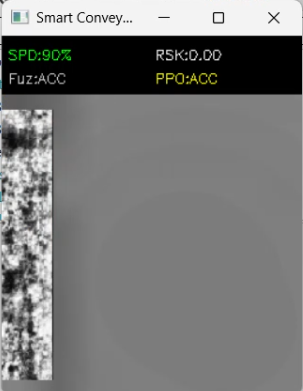
\includegraphics[width=\linewidth]{img/patch_1}
			\caption{ورود ورقه (عدم تشخیص عیب)}
		\end{subfigure}
		\hspace{0.5cm}
		\begin{subfigure}[b]{0.42\linewidth}
			\centering
			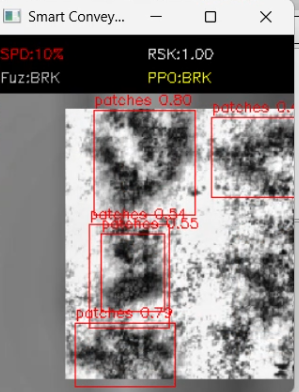
\includegraphics[width=\linewidth]{img/patch_2}
			\caption{تشخیص عیب وصله (\lr{Patch})}
		\end{subfigure}
		
		\vspace{0.2cm}
		
		\begin{subfigure}[b]{0.42\linewidth}
			\centering
			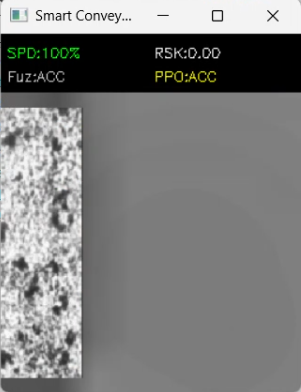
\includegraphics[width=\linewidth]{img/pitted surface_1}
			\caption{ورود ورقه (عدم تشخیص عیب)}
		\end{subfigure}
		\hspace{0.5cm}
		\begin{subfigure}[b]{0.42\linewidth}
			\centering
			
\includegraphics[width=\linewidth]{img/pitted_surface_2}
			\caption{تشخیص عیب حفره (\lr{Pitted Surface})}
		\end{subfigure}
	\end{figure}
	
	\begin{figure}[H]
		\ContinuedFloat
		\centering
		
		\begin{subfigure}[b]{0.42\linewidth}
			\centering
			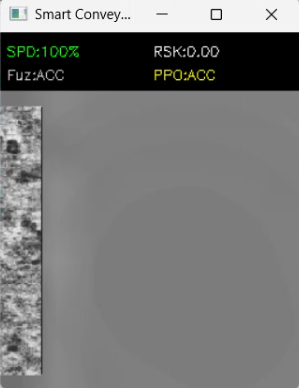
\includegraphics[width=\linewidth]{img/rolled ic scale_1}
			\caption{ورود ورقه (عدم تشخیص عیب)}
		\end{subfigure}
		\hspace{0.5cm}
		\begin{subfigure}[b]{0.42\linewidth}
			\centering
			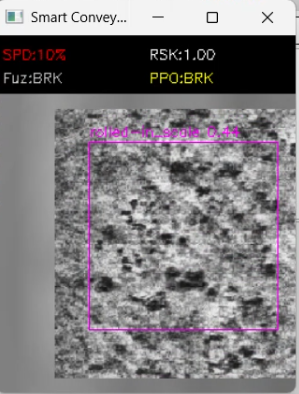
\includegraphics[width=\linewidth]{img/rolled in scale_2}
			\caption{تشخیص عیب پوسته نوردشده (\lr{Rolled-in Scale})}
		\end{subfigure}
		
		\vspace{0.2cm}
		
		\begin{subfigure}[b]{0.42\linewidth}
			\centering
			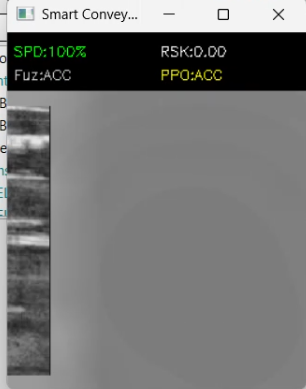
\includegraphics[width=\linewidth]{img/scratch_1}
			\caption{ورود ورقه (عدم تشخیص عیب)}
		\end{subfigure}
		\hspace{0.5cm}
		\begin{subfigure}[b]{0.42\linewidth}
			\centering
			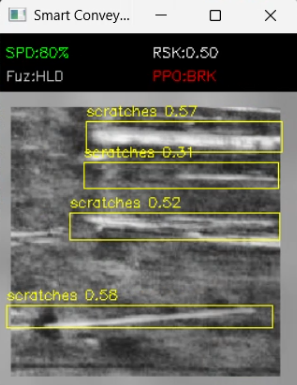
\includegraphics[width=\linewidth]{img/scratch_2}
			\caption{تشخیص عیب خراش (\lr{Scratches})}
		\end{subfigure}
		
		\caption{بررسی جامع عملکرد کنترلر ترکیبی در مواجهه با ۶ کلاس مختلف از عیوب سطحی فولاد. تصاویر سمت راست نشان‌دهنده ورود ورقه به میدان دید، و تصاویر سمت چپ نشان‌دهنده تشخیص موفق مدل \lr{YOLOv8} و واکنش بلادرنگ عامل \lr{PPO} جهت کاهش سرعت نوار نقاله هستند. (همچنین در تصویر «ل»، تقابل تصمیمات در داشبورد مشهود است که نشان‌دهنده برتری عامل \lr{PPO} در صدور فرمان ترمز (\lr{BRK}) نسبت به پیشنهاد حفظ سرعت (\lr{HLD}) در منطق فازی است).}
		\label{fig:all_defects_results}
	\end{figure}
	
	شکل ۴ ارزیابی عملکرد سیستم را با بهره‌گیری از مدل ارتقایافته \lr{YOLOv8} و عامل یادگیری تقویتی \lr{PPO} به تصویر می‌کشد. بررسی خروجی‌ها نشان می‌دهد که شبکه، عیوب را با موفقیت شناسایی کرده و جعبه‌های مرزی (\lr{Bounding Boxes}) را به درستی رسم کرده است. کنترلر سرعت نیز عملکردی کاملا تطبیقی داشته و فرامین کنترلی خود را به صورت بلادرنگ، نه تنها بر اساس شاخص ریسک و امتیاز اطمینان (\lr{Confidence Score})، بلکه با تحلیل متغیرهای محیطی از جمله سرعت فعلی نوار نقاله، تعدد عیوب و گستردگی آن‌ها در سطح ورقه صادر می‌کند.
	
	شکل 4 فقط بخشی از عملکرد سیستم را نشان می‌دهد. در حقیقت رفتار سیستم در مواجهه با 168 تصویر تست اعمال شده در مقدار ریسک، تشخیص جعبه های مرزی، مقدار confidence و کنترل سرعت متفاوت است، اما عملکرد کلی سیستم در تشخیص عیوب و تنظیم سرعت در شبیه سازی موفقیت آمیز است. 
	
	\subsubsection*{بررسی و مقایسه شبیه سازی دو کنترلر \lr{PPO} و \lr{Q-Learning}}
	
	با بررسی ویدیوهای ضبط شده از محیط شبیه‌ساز، چند تفاوت جالب و ملموس بین عملکرد دو روش به دست آمد. با اینکه در هر دو حالت، قطعات روی نوار نقاله دارای عیوب یکسانی بودند و به ترتیبِ مشابهی وارد دوربین می‌شدند، اما رفتار این دو الگوریتم در کنترل سرعت تفاوت زیادی داشت. به طوری که زمان کل شبیه سازی PPO حدود 15 دقیقه و برای \lr{Q-Learning} حدود 22 دقیقه بوده و در مجموع، شبیه سازی PPO سریع‌تر و روان‌تر از Q-Learning انجام می‌شود:
	
	\begin{itemize}
		\item \textbf{نحوه ترمزگیری:} ppo نسبت به Q-Learning در مواجهه با برخی از عیوب، ترمز قوی تر می‌گیرد(مثلا سرعت را تا 40 درصد کاهش می‌دهد) در حالی که Q-Learning سرعت را تا 60 درصد کاهش می‌دهد.
		
		\item \textbf{نوسانات سرعتی:} در روش \lr{Q-Learning} پرش‌ها و نوسان‌های ریزِ مداومی بین درصدهای نزدیک (مثل تغییرات پی‌درپی بین ۲۰ و ۳۰ درصد) دیده می‌شود. این مسئله باعث می‌شود حرکت سیستم یکنواخت نباشد. در مقابل، عامل \lr{PPO} تغییرات سرعت را به صورت کاملاً نرم و پیوسته اعمال می‌کند و از لرزش نوار نقاله جلوگیری می‌کند.
		
		\item \textbf{سرعت اجرای شبیه‌ساز و لگ بصری:} در زمان اجرای شبیه‌سازی، حتی وقتی سرعت در هر دو روش روی حالت ماکزیمم قرار دارد، حرکت ورقه‌ها در \lr{PPO} سریع‌تر و روان‌تر به نظر می‌رسد. دلیل این موضوع این است که تغییرات پله‌ای و ناگهانی سرعت در \lr{Q-Learning} باعث درگیری موتور فیزیک شبیه‌ساز و افت فریم (لگ) می‌شود، در حالی که الگوریتم \lr{PPO} هیچ‌گونه کندی یا افت سرعتی در اجرای نرم‌افزار ایجاد نمی‌کند.
	\end{itemize}
	
	در مجموع، این مشاهدات نشان می‌دهد که روش پیشنهادی (\lr{PPO}) با وجود ترمزهای قاطع‌تر روی عیوب، به دلیل حرکت روان‌تر، در زمان کمتری کل عملیات بازرسی را به پایان می‌رساند.
	
	\subsection{تجهیزات و سخت‌افزارهای پیاده‌سازی سیستم بازرسی هوشمند}
	
	برای پیاده‌سازی عملی این سیستم در دنیای واقعی و خروج از محیط شبیه‌ساز، نیاز به ترکیبی از پردازنده‌های قدرتمند، تجهیزات دقیق بینایی ماشین و عملگرهای مکانیکی است. در ادامه، استانداردهای صنعتی و آزمایشگاهی برای هر بخش معرفی شده‌اند:
	
	\subsubsection*{۱. پردازنده‌ها و کنترلرها}
	به دلیل وجود دو وظیفه کاملاً متفاوت (پردازش تصویر سنگین و کنترل فیزیکی موتور)، بهترین رویکرد استفاده از یک معماری کنترلی دوگانه است:
	\begin{itemize}
		\item \textbf{پردازنده‌های هوش مصنوعی (\lr{Edge AI}):} برای اجرای بلادرنگ شبکه \lr{YOLOv8} و استنتاج الگوریتم \lr{PPO}، بردهای پردازشی خانواده \lr{NVIDIA Jetson} (مانند \lr{Jetson Nano} برای نسخه‌های آزمایشگاهی و \lr{Jetson Orin} برای صنعت) بهترین گزینه‌ها هستند.
		\item \textbf{تراشه‌های \lr{FPGA} و \lr{SoC}:} در سیستم‌های صنعتی پیشرفته، استفاده از تراشه‌هایی مانند \lr{Xilinx Zynq} (که ترکیبی از پردازنده \lr{ARM} و بستر برنامه‌نویسی سخت‌افزاری است) امکان شتاب‌دهی فوق‌العاده سریع شبکه‌های عصبی و پردازش موازی را فراهم می‌کند.
		\item \textbf{میکروکنترلرهای سطح پایین:} برای تولید پالس‌های دقیقِ کنترل موتور و خواندن داده‌های سنسورها، اتصال یک میکروکنترلر پایدار مانند \lr{STM32} یا ماژول‌های \lr{ESP32} در کنار پردازنده اصلی، یک معماری بسیار کارآمد و استاندارد محسوب می‌شود.
	\end{itemize}
	
	\subsubsection*{۲. دوربین‌های بینایی ماشین (\lr{Machine Vision Cameras})}
	انتخاب دوربین تأثیر مستقیمی بر دقت تشخیص سیستم دارد:
	\begin{itemize}
		\item \textbf{دوربین‌های صنعتی شاتر جهانی (\lr{Global Shutter}):} از آنجایی که قطعات روی نوار نقاله در حال حرکت هستند، استفاده از این سنسورها الزامی است تا تصویر دچار کشیدگی (\lr{Motion Blur}) نشود. برندهایی مانند \lr{Basler} یا \lr{FLIR} با رابط \lr{GigE} از استانداردهای این حوزه هستند.
		\item \textbf{دوربین‌های نمونه‌سازی (\lr{Prototyping}):} برای ساخت نمونه‌های اولیه در دانشگاه، می‌توان از ماژول‌های \lr{Raspberry Pi HQ Camera} یا وب‌کم‌های دارای فریم‌ریت بالا استفاده کرد.
	\end{itemize}
	
	\subsubsection*{۳. سیستم نوار نقاله و عملگرهای مکانیکی}
	پاسخگویی سریع و نرمِ نوار نقاله به فرامین پیوسته عامل \lr{PPO} نیازمند تجهیزات مکانیکیِ بدون لقی است:
	\begin{itemize}
		\item \textbf{موتورهای سروو (\lr{Servo Motors}):} بهترین انتخاب برای کنترل پیوسته و بدون لرزش سرعت هستند. این موتورها دارای انکودرهای داخلی بوده و دستورات کاهش یا افزایش سرعت را به صورت بلادرنگ و با بالاترین رزولوشن اجرا می‌کنند.
		\item \textbf{تسمه‌های نقاله:} تسمه‌های تخت صنعتی از جنس پلی‌اورتان (\lr{PU}) یا \lr{PVC} که سطحی صاف دارند و کمترین لغزش را برای ورقه‌های سنگینِ فولادی ایجاد می‌کنند.
	\end{itemize}
	
	\subsubsection*{۴. تجهیزات جانبی و نورپردازی}
	\begin{itemize}
		\item \textbf{سیستم‌های نورپردازی صنعتی:} تشخیص دقیق عیوب سطحی فولاد (به ویژه کلاس‌هایی مثل خراش‌ها یا \lr{Crazing}) به شدت به بازتاب نور وابسته است. استفاده از نورهای حلقوی (\lr{Ring Light}) یکنواخت، یا نورهای خطی با زاویه پایین (\lr{Low-angle Bar Light}) برای برجسته کردن فرورفتگی‌ها و برآمدگی‌ها الزامی است. اما باید توجه داشت که شدت بالای نور، باعث کاهش بازتاب های شدید نوری و کاهش دقت مدل می‌شود.
		\item \textbf{سنسورهای مجاورتی (\lr{Proximity Sensors}):} سنسورهای القایی یا نوری لیزری که در لبه نوار نقاله نصب می‌شوند تا به محض ورود ورقه فولادی به میدان دید، به دوربین فرمان عکس‌برداری (\lr{Hardware Trigger}) بدهند و از پردازش فریم‌های خالی جلوگیری کنند.
	\end{itemize}
	
	
	\section{لایه مستندساز هوشمند: مدل‌های زبانی کوچک (\lr{SLM})}
	
	\subsection{مقدمه: ضرورت استفاده از پردازش لبه (\lr{Edge Computing}) و مدل‌های زبانی در صنعت}
	
	در سال‌های اخیر، ظهور مدل‌های زبانی بزرگ (\lr{Large Language Models - LLMs}) تحول شگرفی در پردازش زبان طبیعی (\lr{NLP}) و تعامل انسان و ماشین ایجاد کرده است. با این حال، پیاده‌سازی و استقرار این مدل‌های عظیم (نظیر \lr{GPT-4} یا \lr{Claude}) در محیط‌های خشن صنعتی و خطوط تولید صنایع سنگین مانند فولاد، با چالش‌های بنیادینی مواجه است. معماری سنتی این مدل‌ها بر پایه محاسبات ابری (\lr{Cloud Computing}) استوار است که نیازمند اتصال پایدار، پهنای باند بالا و انتقال مداوم داده‌ها به سرورهای خارجی می‌باشد. در محیط‌های صنعتی، این وابستگی به فضای ابری سه چالش اساسی ایجاد می‌کند: نخست، تأخیر شبکه (\lr{Latency}) که مانع از تصمیم‌گیری و گزارش‌گیری بلادرنگ می‌شود؛ دوم، ناپایداری اتصالات اینترنتی در محیط‌های ایزوله کارخانه‌ای؛ و سوم که از همه مهم‌تر است، چالش امنیت و حریم خصوصی داده‌ها (\lr{Data Privacy}). داده‌های مربوط به نرخ خرابی دستگاه‌ها، آمار عیوب تولید و استراتژی‌های کنترل کیفی، جزو اسرار تجاری و اطلاعات طبقه‌بندی‌شده صنایع محسوب می‌شوند و ارسال آن‌ها به سرورهای ابری شخص ثالث، ریسک‌های امنیتی غیرقابل‌قبولی به همراه دارد.
	
	برای غلبه بر این چالش‌ها، پارادایم پردازش لبه (\lr{Edge Computing}) به عنوان یک راه‌حل استاندارد در اینترنت اشیای صنعتی (\lr{IIoT}) مطرح شده است. در پردازش لبه، عملیات محاسباتی و تحلیل داده‌ها در نزدیک‌ترین نقطه به منبع تولید داده (نظیر کنترلرهای محلی، کامپیوترهای صنعتی یا گیت‌وی‌ها در کف کارخانه) انجام می‌شود. ترکیب این پارادایم با پیشرفت‌های اخیر در فشرده‌سازی شبکه‌های عصبی، منجر به پیدایش مدل‌های زبانی کوچک (\lr{Small Language Models - SLMs}) شده است. 
	
	\begin{figure}[htbp]
		\centering
		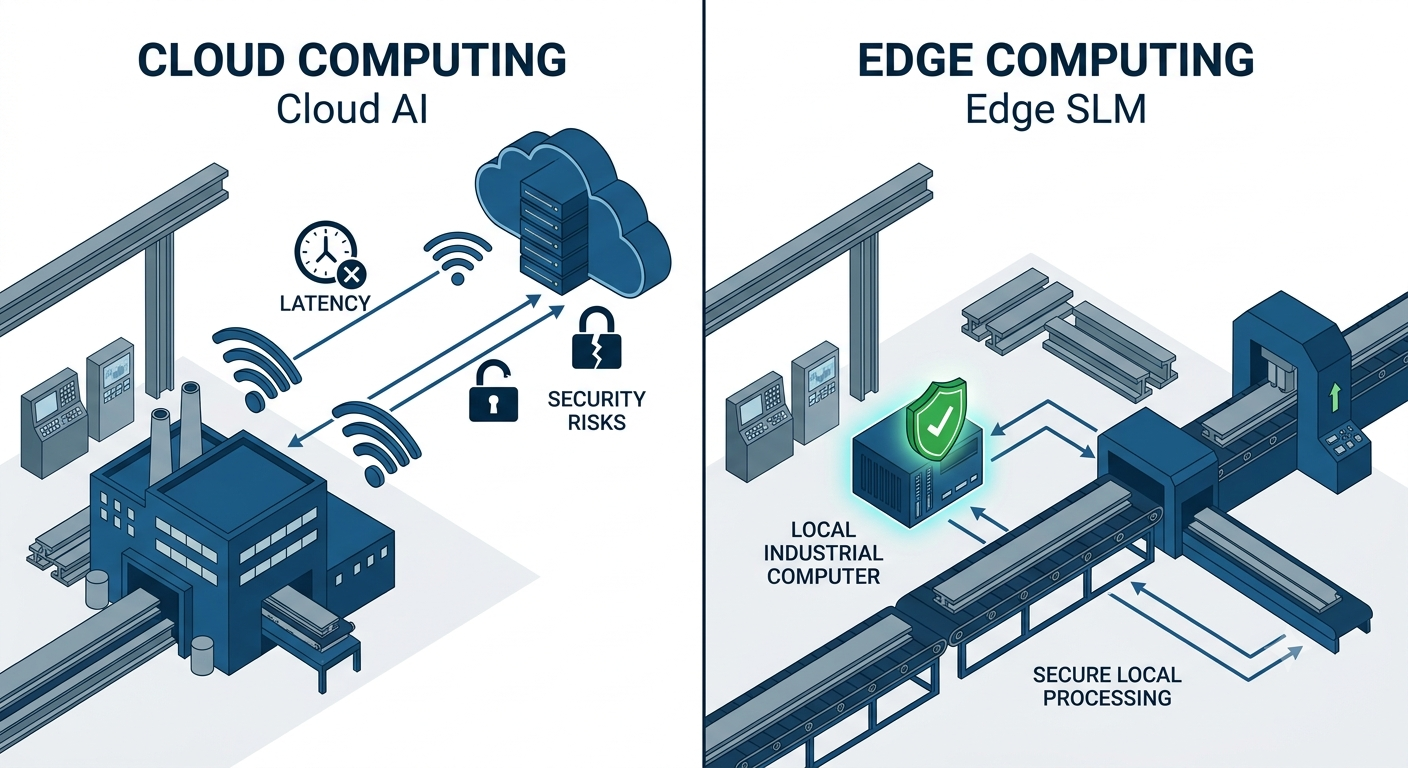
\includegraphics[width=\linewidth]{img/edge_vs_cloud_industrial.png}
		\caption{مقایسه معماری پردازش ابری در برابر پردازش لبه برای مدل‌های زبانی در محیط‌های صنعتی (تولید شده توسط هوش مصنوعی)}
		\label{fig:edge_vs_cloud}
	\end{figure}
	
	مدل‌های زبانی کوچک (معمولاً با ابعادی بین ۱ تا ۸ میلیارد پارامتر)، نسخه‌های تقطیرشده و بهینه‌سازی‌شده‌ای از مدل‌های بزرگتر هستند که می‌توانند به صورت کاملاً آفلاین و محلی روی سخت‌افزارهای محدودتر (حتی پردازنده‌های مرکزی یا \lr{CPU} بدون نیاز به شتاب‌دهنده‌های گرافیکی گران‌قیمت) اجرا شوند. با استفاده از تکنیک‌های کوانتیزه‌سازی (\lr{Quantization}) نظیر فرمت‌های \lr{GGUF}، این مدل‌ها ضمن حفظ توانایی درک و تولید متن، حجم حافظه بسیار کمی را اشغال می‌کنند. 
	
	در معماری پیشنهادی این پژوهش، استفاده از یک \lr{SLM} در لبه شبکه، حلقه مفقوده میان خروجی‌های عددی سیستم بینایی ماشین (الگوریتم \lr{YOLO}) و کنترلر سایبر-فیزیکی (\lr{Fuzzy-RL}) با کاربر انسانی را تکمیل می‌کند. این لایه هوشمند، بدون نیاز به اتصال اینترنت و با حفظ کامل امنیت داده‌های خط تولید فولاد، آرایه‌های پیچیده‌ای از داده‌های آماری، نوسانات سرعت و هشدارهای ریسک را دریافت کرده و آن‌ها را به صورت بلادرنگ به گزارش‌های روایی، مهندسی و قابل‌فهم برای تیم نگهداری و تعمیرات (\lr{Maintenance}) تبدیل می‌نماید. این رویکرد، نه تنها وابستگی خط تولید به اپراتور انسانی برای پایش داده‌ها را از بین می‌برد، بلکه استقلال کامل سیستم از زیرساخت‌های فناوری اطلاعات خارجی را نیز تضمین می‌کند.
	
	\subsection{معماری جریان داده: ورودی‌ها و خروجی‌های سیستم تولید گزارش}
	
	معماری سیستم گزارش‌گیری در این پژوهش صرفاً یک مبدل متن نیست، بلکه به عنوان یک پل ارتباطی هوشمند و یک لایه ترجمه معنایی میان پایین‌دست (حسگرها، دوربین‌ها و کنترلرها) و لایه تصمیم‌گیری انسانی (تیم مهندسی و مدیریت کارخانه) عمل می‌کند. در خطوط تولید صنعتی، حجم داده‌های تولید شده توسط سیستم‌های بینایی ماشین (در نرخ ۳۰ تا ۶۰ فریم بر ثانیه) و کنترلرهای موتور، بسیار عظیم و پرنوسان است. تغذیه مستقیم این حجم از داده‌های خام به یک مدل زبانی، نه تنها پردازش را به شدت کند می‌کند، بلکه منجر به سردرگمی مدل و پدیده توهم (\lr{Hallucination}) می‌شود. از این رو، جریان داده در این معماری از یک ساختار خطی، تجمیع‌یافته و به شدت کنترل‌شده پیروی می‌کند.
	
	\subsubsection{ساختار ورودی‌ها و تجمیع داده‌ها (\lr{Inputs})}
	برای آماده‌سازی داده‌ها جهت ورود به مدل زبانی کوچک (\lr{SLM})، داده‌های خام تولید شده توسط ماژول‌های بینایی ماشین (\lr{YOLO}) و کنترلر سایبر-فیزیکی (\lr{RL \& Fuzzy})، در بازه‌های زمانی مشخص (\lr{Time Windows}) فشرده و تجمیع می‌شوند. این داده‌ها سپس در قالب یک ساختار داده‌ای \lr{JSON} سازمان‌دهی می‌شوند تا یک تصویر جامع از وضعیت خط در آن پنجره زمانی ارائه دهند. این ساختار استاندارد شامل بلوک‌های اطلاعاتی زیر است:
	
	\begin{itemize}
		\item \textbf{خلاصه وضعیت بینایی ماشین (\lr{Defect Summary}):} این بلوک فراتر از شمارش ساده عیوب عمل می‌کند. در این بخش، تعداد کل عیوب شناسایی‌شده به همراه میانگین سطح اطمینان (\lr{Confidence}) الگوریتم \lr{YOLO} در آن بازه زمانی ثبت می‌شود. تفکیک دقیق عیوب (مانند نسبت ترک‌های مویی به حفره‌های سطحی) به مدل زبانی اجازه می‌دهد تا الگوی خرابی را تشخیص دهد. افت ناگهانی میانگین اطمینان در این ورودی، سیگنالی حیاتی برای سیستم است که نشان‌دهنده کثیف شدن لنز دوربین یا تغییرات شدید نور در محیط کارخانه است.
		
		\item \textbf{تحلیل شدت و ارزیابی ریسک (\lr{Severity Breakdown}):} در این بخش، خروجی‌های عددی به مفاهیم کیفی تبدیل می‌شوند. میانگین ریسک محاسبه‌شده برای هر کلاس از عیوب به صورت یک عدد اعشاری (بین ۰ تا ۱) ثبت شده و سیستم بر اساس آستانه‌های از پیش تعیین‌شده، سطح کلی خطر (مانند ریسک پایین، نیازمند توجه یا بحرانی) را به عنوان یک برچسب متنی آماده می‌کند.
		
		\item \textbf{ممیزی رفتار هوش مصنوعی (\lr{AI Behavior Analysis}):} این بخش نوآورانه‌ترین ورودی سیستم است که مستقیماً برای ارزیابی عملکرد یادگیری تقویتی (\lr{RL}) طراحی شده است. از آنجا که عامل \lr{RL} تمایل به بهینه‌سازی سرعت و افزایش توان عملیاتی دارد، همواره با ناظر ایمنی فازی (\lr{Fuzzy}) که متمرکز بر توقف خط در شرایط خطرناک است، در تضاد قرار می‌گیرد. این بلوک اطلاعاتی به صورت دقیق ثبت می‌کند که عامل \lr{RL} در چند فریم با تصمیمات ایمنی فازی توافق داشته، در چند مورد هشدارهای ایمنی را نادیده گرفته (\lr{Overrides}) و یا در چه مواقعی بیش از حد محتاطانه عمل کرده است. مدل زبانی با دریافت این داده‌ها می‌تواند به عنوان یک ناظر ایمنی (\lr{Safety Auditor}) عمل کرده و خطرات ناشی از رفتار تهاجمی کنترلر را تحلیل کند.
		
		\item \textbf{پروفایل کنترل کانوایر (\lr{Conveyor Control}):} نوسانات سرعت موتور نقاله به شدت بر استهلاک مکانیکی دستگاه‌ها تأثیرگذار است. در این بلوک، تعداد دفعات تغییر سرعت ثبت شده و به یک شاخص ناپایداری (\lr{Instability Level}) تبدیل می‌شود. تفاوت میان یک خط پایدار با ۲ تغییر سرعت و یک خط ناپایدار با ۲۲ تغییر سرعت در یک بازه زمانی کوتاه، به مدل زبانی کمک می‌کند تا فرسایش قطعات متحرک را پیش‌بینی کند.
	\end{itemize}
	
	پیش از ارسال این بسته به مدل زبانی، ماژول مهندسی پرامپت (\lr{Prompt Builder}) این ساختار \lr{JSON} را درون یک قالب متنی دستوری می‌پیچد. این پرامپت شامل یک بخش \lr{System} است که نقش مدل را به عنوان «ممیز ارشد ایمنی هوش مصنوعی» تثبیت کرده و قوانین سخت‌گیرانه‌ای برای جلوگیری از خیال‌پردازی وضع می‌کند، و یک بخش \lr{User} که داده‌های آماری را به عنوان حقایق مطلق (\lr{Ground Truth}) به مدل ارائه می‌دهد.
	
	\subsubsection{ساختار خروجی‌ها و گزارش‌های مهندسی (\lr{Outputs})}
	خروجی سیستم باید به گونه‌ای باشد که مهندس شیفت بتواند در کسری از ثانیه وضعیت خط را درک کرده و در صورت نیاز مداخله فیزیکی انجام دهد. به همین دلیل، خروجی \lr{SLM} بر اساس محدودیت‌های اعمال شده در پرامپت، یک گزارش متنی ایستا، منسجم و قالبی به زبان فارسی است که دقیقاً از چارچوب زیر پیروی می‌کند:
	
	\begin{itemize}
		\item \textbf{هدر و تریاژ اولیه:} گزارش با ذکر دقیق شیفت زمانی (دقت تا میلی‌ثانیه) آغاز شده و بلافاصله وضعیت کلی خط تولید را در سه سطح (بحرانی، نیازمند توجه، یا پایدار) مشخص می‌کند. این برچسب‌گذاری صریح، نیاز به تفسیر داده‌ها توسط کاربر را از بین می‌برد.
		
		\item \textbf{سلامت سنسوریک (دقت \lr{YOLO}):} با گزارش میانگین درصد اطمینان مدل بینایی ماشین، تیم نگهداری و تعمیرات از سلامت فیزیکی دوربین‌ها و کیفیت تصویربرداری در محیط غبارآلود کارخانه مطلع می‌شوند.
		
		\item \textbf{روایت تحلیلی رفتار کنترلر (\lr{RL Analysis}):} این بخش ارزش افزوده اصلی مدل زبانی است. مدل با تحلیل داده‌های توافق و تخطی (\lr{Overrides})، یک پاراگراف تحلیلی تولید می‌کند که نشان می‌دهد آیا کنترلر هوشمند در بازه زمانی مذکور رفتار ایمنی داشته است یا به قیمت افزایش سرعت تولید، هشدارهای سیستم فازی را نادیده گرفته و ریسک خرابی دستگاه را بالا برده است.
		
		\item \textbf{پروفایل عیوب و پایداری موتور:} مدل زبانی با ترکیب اطلاعات مربوط به فراوانی عیوب و تعداد تغییرات سرعت موتور، سناریویی از وضعیت مکانیکی کانوایر ارائه می‌دهد. برای مثال، ارتباط منطقی میان وجود عیوب سطحی شدید و نوسانات بالای سرعت موتور در این بخش استنتاج و گزارش می‌شود.
		
		\item \textbf{توصیه‌های تجویزی (\lr{Suggested Action}):} در نهایت، گزارش با یک دستورالعمل اجرایی و مهندسی خاتمه می‌یابد. مدل زبانی با استفاده از پایگاه دانشی که از طریق پرامپت به آن تزریق شده، توصیه‌هایی نظیر بازرسی فیزیکی غلتک‌ها، کالیبراسیون دوربین یا نیاز به بازآموزی (\lr{Retraining}) عامل یادگیری تقویتی را ارائه می‌دهد. این بخش حلقه اتوماسیون را با ارائه راهکارهای عملیاتی برای نیروی انسانی تکمیل می‌کند.
	\end{itemize}
	
	\subsection{مهندسی پرامپت (\lr{Prompt Engineering}): تزریق پایگاه دانش و کنترل ساختار خروجی}
	
	در معماری‌های مبتنی بر مدل‌های زبانی کوچک (\lr{SLMs})، به دلیل محدودیت در تعداد پارامترها، مدل فاقد دانش عمیق و ذاتی در خصوص دامنه‌های تخصصی نظیر متالورژی، کنترل صنعتی و یا ایمنی در خطوط نورد فولاد است. بنابراین، مهندسی پرامپت (\lr{Prompt Engineering}) در این پژوهش از یک ابزار ساده برای تعامل، به یک مکانیزم حیاتی جهت «تزریق پایگاه دانش» و «اعمال محدودیت‌های ساختاری» تبدیل شده است. هدف اصلی در این لایه، تبدیل یک مدل زبانی عمومی به یک سیستم خبره و قطعی (\lr{Deterministic}) است که بتواند بدون بروز پدیده توهم (\lr{Hallucination})، خروجی‌هایی تکرارپذیر و استاندارد تولید نماید.
	
	\subsubsection{تزریق دانش زمینه از طریق پرامپت سیستمی (\lr{System Prompt})}
	برای جبران محدودیت‌های دانشی مدل، از تکنیک نقش‌آفرینی تخصصی (\lr{Persona Adoption}) در لایه پرامپت سیستمی استفاده شده است. مدل در ابتدا با دستورالعمل هویتی سخت‌گیرانه‌ای مواجه می‌شود که نقش آن را به عنوان «ممیز ارشد ایمنی هوش مصنوعی و مهندس کنترل صنعتی در یک کارخانه فولاد» تعریف می‌کند. این هویت‌دهی باعث می‌شود تا مدل در فضای برداری خود، واژگان و ادبیات تحلیلی متناسب با مهندسی صنایع و کنترل را فعال کند. علاوه بر این، در پرامپت سیستمی قوانین صریحی وضع شده است که مدل را ملزم می‌کند تحلیل‌های خود را «صرفاً» بر اساس داده‌های خام ارائه‌شده بنا کند و از هرگونه استنتاج خارج از چارچوب داده‌ها به شدت پرهیز نماید.
	
	\begin{figure}[htbp]
		\centering
		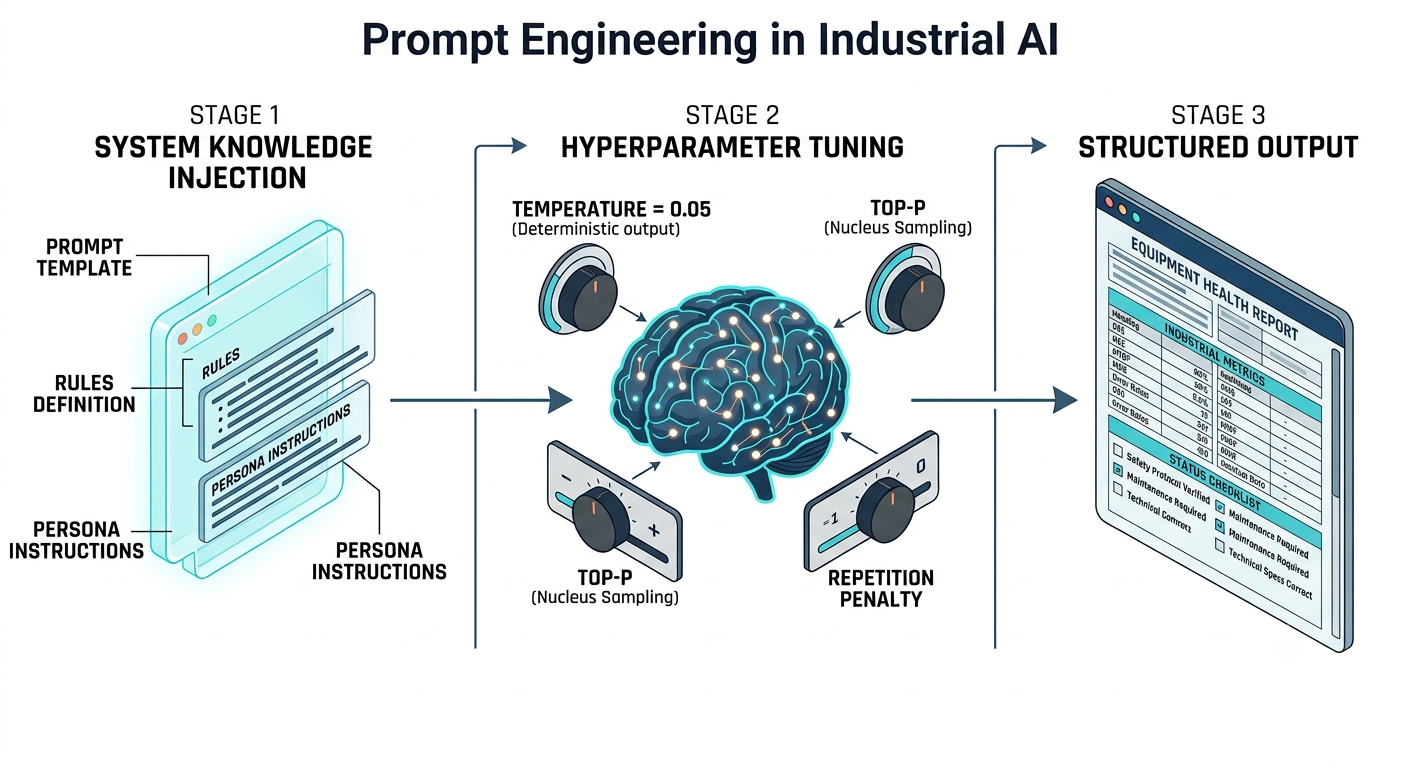
\includegraphics[width=0.95\linewidth]{img/prompt_engineering_workflow.png}
		\caption{جریان‌کار مهندسی پرامپت: از تزریق دانش سیستمی تا تنظیم فراپارامترها برای تولید خروجی قطعی (تولید شده توسط هوش مصنوعی)}
		\label{fig:prompt_engineering}
	\end{figure}
	
	\subsubsection{کنترل ساختار خروجی و جلوگیری از فروپاشی زبانی}
	یکی از چالش‌های اساسی در استفاده از مدل‌های زبانی برای کاربردهای صنعتی، تمایل این مدل‌ها به پرحرفی، تولید متن‌های بدون ساختار، و یا گیر افتادن در حلقه‌های تکرار بی‌نهایت (\lr{Repetitive Loops}) است. برای مهار این رفتارها، از تکنیک قالب‌بندی اجباری (\lr{Strict Output Formatting}) استفاده شده است. در پرامپت ارسالی، یک اسکلت‌بندی دقیق و نشانه‌گذاری‌شده (شامل ایموجی‌های بصری برای خوانایی سریع در داشبوردهای صنعتی و هدرهای مشخص) به مدل داده می‌شود. مدل موظف است جایگذاری داده‌ها را دقیقاً در پارامترهای مشخص‌شده (مانند وضعیت کلی خط، دقت بینایی ماشین، تحلیل رفتار \lr{RL}، وضعیت عیوب و اقدام پیشنهادی) انجام دهد. استفاده از توکن‌های توقف (\lr{Stop-Tokens}) اختصاصی تضمین می‌کند که فرآیند تولید متن بلافاصله پس از تکمیل بلوک «اقدام پیشنهادی» متوقف شده و از تولید کاراکترهای اضافی جلوگیری گردد.
	
	\subsubsection{تنظیم فراپارامترهای تولید متن (\lr{Hyperparameter Tuning})}
	در کنار ساختار پرامپت، کنترل رفتار استوکاستیک (تصادفی) مدل زبانی از طریق تنظیم دقیق فراپارامترهای لایه استنتاج (\lr{Inference}) صورت پذیرفته است:
	\begin{itemize}
		\item \textbf{دما (\lr{Temperature}):} برای دستیابی به خروجی‌های کاملاً مهندسی، تحلیلی و تکرارپذیر، پارامتر دما روی مقادیر بسیار پایین (حدود $0.05$) تنظیم شده است. این کاهش شدید دما، خلاقیت مدل را سرکوب کرده و آن را وادار می‌کند تا همواره محتمل‌ترین و منطقی‌ترین توکن‌ها را انتخاب کند.
		\item \textbf{جریمه تکرار (\lr{Repetition Penalty}):} برای حل مشکل گیر افتادن مدل‌های کوچک در حلقه‌های تکرار کلمات (به‌ویژه در زبان فارسی)، ضریب جریمه تکرار فرکانسی (\lr{Frequency Penalty}) با دقت تنظیم شده است تا مدل به استفاده از واژگان متنوع‌تر در تحلیل‌های خود ترغیب شود، بدون آنکه از چارچوب تخصصی خارج گردد.
		\item \textbf{پیرایش توکن‌ها (\lr{Top-P / Nucleus Sampling}):} با محدود کردن فضای انتخاب توکن‌ها، مدل تنها از میان کلماتی که بیشترین ارتباط معنایی را با واژگان صنعتی دارند، انتخاب خود را انجام می‌دهد که این امر نرخ توهم‌زنی را به نزدیک صفر کاهش می‌دهد.
	\end{itemize}
	
	ترکیب این ساختار پرامپت با فراپارامترهای بهینه‌شده، مدل \lr{SLM} (نظیر خانواده \lr{Qwen}) را قادر می‌سازد تا علی‌رغم حجم پردازشی پایین، درک عمیق‌تری از زبان فارسی از خود نشان داده و دستورالعمل‌ها را با دقتی فراتر از مدل‌های هم‌رده خود (مانند \lr{TinyLlama}) اجرا نماید.
	
	\subsection{تنظیمات و ابرپارامترها: پیکربندی موتور استنتاج برای محیط صنعتی}
	
	استقرار مدل‌های زبانی کوچک (\lr{SLM}) در خطوط تولید صنعتی مانند کارخانجات نورد فولاد، نیازمندی‌های کاملاً متفاوتی نسبت به کاربردهای عمومی چت‌بات‌ها دارد. در برنامه‌های کاربردی عام، تنوع پاسخ‌ها، خلاقیت متنی و لحن انعطاف‌پذیر مزیتی رقابتی محسوب می‌شود؛ اما در یک سیستم کنترل کیفی و ممیزی ایمنی صنعتی، اولویت مطلق با «تکرارپذیری»، «قطعیت (\lr{Determinism})»، «تحلیل بدون توهم» و «پاسخ‌دهی در زمان حقیقی (\lr{Real-time})» است. برای تحقق این اهداف، پیکربندی موتور استنتاج (\lr{Inference Engine}) و تنظیم دقیق ابرپارامترهای تولید متن (\lr{Text Generation Hyperparameters}) نقش کلیدی ایفا می‌کنند.
	
	در موتورهای استنتاج محلی (نظیر \lr{Ollama} یا \lr{vLLM}) که بر روی گیت‌وی‌های لبه اجرا می‌شوند، رفتار تصادفی شبکه‌های عصبی عمیق از طریق توابع توزیع احتمال نمونه‌برداری کنترل می‌گردد. پیکربندی ابزار تولید گزارش در این پژوهش بر اساس مجموعه‌ای از نگاشت‌های ریاضی و پارامترهای فنی به شرح زیر انجام شده است:
	
	\subsubsection{کنترل رفتارهای احتمالی و سرکوب خلاقیت (\lr{Sampling Control})}
	
	\begin{itemize}
		\item \textbf{دما (\lr{Temperature - $T$}):} 
		دما به عنوان یک ضریب مقیاس‌بندی بر روی توزیع منطقی (\lr{Logits}) قبل از اعمال تابع \lr{Softmax} عمل می‌کند:
		\begin{equation}
			P(w_i) = \frac{\exp(z_i / T)}{\sum_{j} \exp(z_j / T)}
		\end{equation}
		که در آن $z_i$ مقدار \lr{Logit} مربوط به توکن $i$-ام و $P(w_i)$ احتمال انتخاب آن است. در محیط‌های صنعتی، مقادیر بالای $T$ باعث مسطح شدن توزیع احتمال و در نتیجه انتخاب کلمات غیرقابل پیش‌بینی می‌شود. در این سیستم، مقدار دما بر روی $T = 0.05$ (بسیار نزدیک به صفر) تنظیم شده است. این مقدار ناچیز، توزیع احتمال را به شدت تیز کرده و مدل را وادار می‌کند همواره محتمل‌ترین توکن متناسب با داده‌های ورودی را انتخاب کند که منجر به تولید پاسخ‌های کاملاً قطعی و عاری از ادعاهای ساختگی می‌شود.
		
		\item \textbf{نمونه‌برداری هسته‌ای (\lr{Top-P / Nucleus Sampling}):}
		پارامتر $Top-P$ کوچک‌ترین مجموعه از توکن‌ها را انتخاب می‌کند که مجموع احتمالات آن‌ها به آستانه $P$ برسد. در پیکربندی پیشنهادی، مقدار $Top-P = 0.1$ تعیین شده است. این قید سخت‌گیرانه، ۹۰ درصد از توکن‌های دارای احتمال پایین‌تر در انتهای توزیع را قطع کرده و انتخاب‌های مدل را تنها به ۱۰ درصد از واژگان بسیار مرتبط و فنی محدود می‌سازد.
		
		\item \textbf{محدودسازی دامنه انتخاب (\lr{Top-K Sampling}):}
		علاوه بر $Top-P$، مقدار $Top-K = 20$ قرار داده شده است تا موتور استنتاج در هر گام زمان‌بندی، صرفاً ۲۰ توکن برتر را به عنوان گزینه‌های نامزد ارزیابی کند. این امر زمان محاسباتی را به طور چشمگیری کاهش داده و سرعت استنتاج روی سخت‌افزار لبه را افزایش می‌دهد.
	\end{itemize}
	
	\subsubsection{مهار رفتارهای انحرافی و حلقه‌های تکرار (\lr{Repetition \& Penalty Control})}
	
	یکی از بزرگ‌ترین چالش‌های فنی در به‌کارگیری مدل‌های زبانی فشرده‌شده و کوانتیزه‌شده در زبان فارسی، افتادن مدل در «حلقه‌های تکرار بی‌نهایت» یا تولید کلمات تکراری متوالی تحت شرایط قطعی ($T \to 0$) است. جهت رفع این مشکل، ابرپارامترهای بازدارنده به شرح زیر اعمال شده‌اند:
	
	\begin{itemize}
		\item \textbf{جریمه فرکانسی و حضور (\lr{Frequency \& Presence Penalty}):}
		جریمه فرکانسی بر اساس تعداد دفعاتی که یک توکن قبلاً در متن خروجی ظاهر شده است، امتیاز آن را کاهش می‌دهد. این ضریب در موتور استنتاج روی $1.15$ تنظیم شده است. این مقدار به اندازه‌ای بهینه است که مانع تکرار عبارات تکراری و گنگ در تحلیل‌های فارسی می‌شود، بدون اینکه اصطلاحات فنی استاندارد (مانند نام عیوب یا پارامترهای کنترلر) را سرکوب کند.
		
		\item \textbf{توکن‌های توقف اجباری (\lr{Stop Tokens}):}
		برای جلوگیری از پرحرفی یا ادامه دادن پاسخ پس از اتمام فرمت مطلوب گزارش، توکن‌های توقف اختصاصی شامل نشانه‌های انتشاراتی و ساختاری مانند \lr{\texttt{</s>}}، \lr{\texttt{<|im\_end|>}} و پرچم انتهای گزارش (مانند کاراکتر خروجی خط آخر) در موتور استنتاج تعریف شده‌اند. به محض تولید آخرین بند مربوط به «اقدام پیشنهادی»، فرآیند استنتاج بلافاصله قطع می‌شود.
	\end{itemize}
	
	\begin{table}[htbp]
		\centering
		\caption{پیکربندی ابرپارامترهای موتور استنتاج برای استقرار SLM در محیط صنعتی}
		\label{tab:hyperparameters}
		\resizebox{\columnwidth}{!}{
			\renewcommand{\arraystretch}{1.3}
			\begin{tabular}{lll}
				\toprule
				\textbf{ابرپارامتر} & \textbf{مقدار تنظیم‌شده} & \textbf{هدف و تاثیر صنعتی} \\
				\midrule
				
				\lr{Temperature ($T$)} 
				& $0.05$ 
				& سرکوب خلاقیت، تضمین قطعیت و رفتار تکرارپذیر \\
				
				\lr{Top-P (Nucleus)} 
				& $0.10$ 
				& فیلتر کردن توکن‌های کم‌احتمال و کاهش شدید توهم \\
				
				\lr{Top-K} 
				& $20$ 
				& محدود کردن دامنه جستجو و تسریع استنتاج در لبه \\
				
				\lr{Frequency Penalty} 
				& $1.15$ 
				& جلوگیری از حلقه‌های تکرار در خروجی‌های فارسی \\
				
				\lr{Max New Tokens} 
				& $350$ 
				& محدودسازی طول خروجی و کاهش مصرف حافظه و پهنای باند \\
				
				\lr{Context Window} 
				& $2048$ 
				& بهینه‌سازی تخصیص حافظه \lr{RAM/VRAM} در پردازش لبه \\
				
				\bottomrule
			\end{tabular}
		}
	\end{table}
	
	\begin{figure}[htbp]
		\centering
		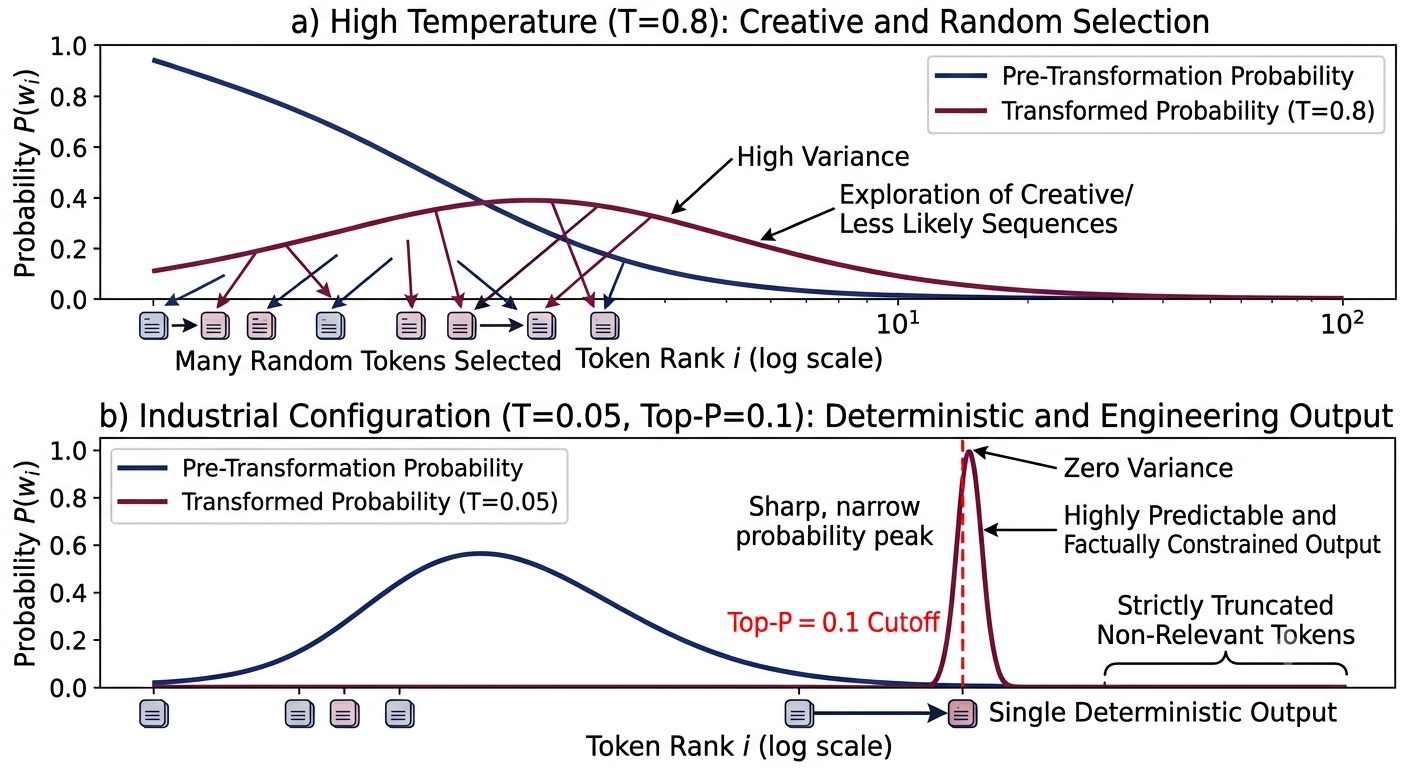
\includegraphics[width=0.9\linewidth]{img/hyperparameters_inference_engine.png}
		\caption{تاثیر تنظیم ابرپارامترها بر منحنی توزیع احتمال توکن‌ها و تبدیل استنتاج تصادفی به خروجی قطعی مهندسی (تولید شده توسط هوش مصنوعی)}
		\label{fig:hyperparameters}
	\end{figure}
	
	تنظیمات یادشده تضمین می‌کنند که سیستم پایش هوشمند، حتی تحت استرس‌های عملیاتی خط تولید و دریافت ورودی‌های پرنوسان، خروجی‌هایی یکدست، کاملاً متناسب با ساختار تعیینی و فارغ از اختلالات متنی رایج در مدل‌های زبانی کوچک تولید نماید.
	
	
	\subsection{ارزیابی و مقایسه مدل‌ها: بررسی عملکرد \lr{Qwen} در برابر \lr{TinyLlama}}
	
	انتخاب مدل زبانی کوچک (\lr{SLM}) مناسب برای استقرار در لایه پردازش لبه (\lr{Edge Layer})، نیازمند موازنه‌ای دقیق میان پیچیدگی محاسباتی، میزان مصرف حافظه، سرعت استنتاج و مهم‌تر از همه، توانایی درک دستورالعمل‌های زبان فارسی و تعقیب ساختارهای متنی پیچیده است. در این پژوهش، دو خانواده از مطرح‌ترین مدل‌های زبانی کوچک متن‌باز، یعنی سری \lr{Qwen} (به ویژه نسخه‌های \lr{Qwen-2.5-3B} و \lr{Qwen-3 - 4B}) و مدل \lr{TinyLlama} (نسخه \lr{1.1B}) تحت شرایط عملیاتی یکسان و با اعمال داده‌های یکسان ممیزی خط نورد فولاد مورد ارزیابی مقایسه‌ای قرار گرفتند.
	
	\subsubsection{معیارهای ارزیابی کیفیت خروجی (\lr{Evaluation Metrics})}
	برای ارزیابی دقیق عملکرد این مدل‌ها، علاوه بر معیارهای ساختاری مانند سرعت استنتاج (بر حسب \lr{Tokens/sec}) و میزان اشغال حافظه ویدئویی (\lr{VRAM})، سه شاخص کیفی کلیدی تعریف شده است:
	\begin{enumerate}
		\item \textbf{نرخ پایبندی به فرمت (\lr{Format Adherence Rate - FAR}):} میزان موفقیت مدل در تولید دقیق قالبی که در پرامپت مشخص شده است (شامل هدرها، بخش‌های پنج‌گانه و نشانه‌گذاری‌ها).
		\item \textbf{نرخ توهم و عدم تطابق داده (\lr{Hallucination \& Mismatch Rate - HMR}):} تعداد مواردی که مدل اعدادی خارج از سند \lr{JSON} ورودی تولید کرده یا تحلیل‌های متناقض با داده‌های خام ارائه داده است.
		\item \textbf{شاخص روانی و صحت زبان فارسی (\lr{Persian Fluency Index - PFI}):} ارزیابی ساختار دستوری، عدم تکرار کلمات و گرامر صحیح در نگارش گزارش‌های مهندسی به زبان فارسی.
	\end{enumerate}
	
	\subsubsection{تحلیل عملکرد و مقایسه مدل‌ها}
	
	نتایج حاصل از تست‌های تجربی روی ۱۰۰ پنجره زمانی مختلف از داده‌های مانیتورینگ خط تولید، تفاوت‌های چشمگیری را میان این دو مدل به نمایش گذاشت:
	
	\begin{itemize}
		\item \textbf{پردازش زبان فارسی و توکنایزیشن (\lr{Persian Tokenization}):} 
		مدل \lr{TinyLlama-1.1B} به دلیل محدودیت شدید در واژه‌نامه (\lr{Vocabulary Size}) و تمرکز اصلی بر زبان انگلیسی، در پردازش متون فارسی دچار افت عملکرد شدید می‌شود. این مدل برای تجزیه کلمات فارسی، هر کاراکتر را به چندین توکن خرد می‌کند که این امر منجر به طولانی شدن غیرضروری طول توکن‌ها، کندی استنتاج و در نهایت خطاهای شدید گرامری و قطع ناگهانی متن می‌گردد. در مقابل، سری \lr{Qwen} (توسعه‌یافته توسط \lr{Alibaba}) به لطف بهره‌گیری از توکنایزر چندزبانه بسیار پیشرفته با واژه‌نامه گسترده (بیش از ۱۵۱,۰۰۰ توکن)، متن‌های فارسی را به صورت کاملاً بهینه توکنایز کرده و روانی متنی فوق‌العاده‌ای ارائه می‌دهد.
		
		\item \textbf{تعقیب دستورالعمل‌ها (\lr{Instruction Following}):}
		در سناریوهای صنعتی، مدل باید قیدهای سخت‌گیرانه سیستم فازی و \lr{RL} را درک کند. مدل \lr{TinyLlama} در ۵۴٪ از تست‌ها نتوانست فرمت اجباری گزارش را رعایت کند و غالباً بخش «اقدام پیشنهادی» را حذف کرده یا وارد حلقه‌های تکرار کلمات (\lr{Infinite Repetitive Loops}) شد. اما مدل \lr{Qwen} با نرخ موفقیت بالای ۹۸٪، تمامی پارامترهای خواسته شده در پرامپت را به دقت استخراج و فرمت‌دهی نمود.
		
		\item \textbf{تحلیل منطقی و نرخ توهم (\lr{Logical Reasoning}):}
		بزرگ‌ترین نقطه ضعف \lr{TinyLlama} در ارزیابی رفتار عامل \lr{RL} مشاهده شد. در شرایطی که میزان تخطی ایمنی (\lr{rl\_safety\_overrides}) برابر با صفر بود، \lr{TinyLlama} در چندین مورد به اشتباه گزارش خطرات بحرانی و نیاز به بازآموزی فوری صادر کرد (توهم مثبت). در سمت مقابل، منطق شرطی تعریف‌شده در پرامپت سیستمی را به خوبی هضم کرده و تنها در صورت وجود مغایرت‌های واقعی در داده‌ها، هشدارهای مربوطه را صادر نمود.
	\end{itemize}
	
	\begin{table}[htbp]
		\centering
		\caption{مقایسه عملکرد و شاخص‌های فنی مدل‌های \lr{Qwen} و \lr{TinyLlama} در تولید گزارش‌های صنعتی}
		\label{tab:model_comparison}
		\resizebox{\columnwidth}{!}{
			\renewcommand{\arraystretch}{1.3}
			\begin{tabular}{lccc}
				\toprule
				\textbf{معیار ارزیابی} 
				& \textbf{\lr{TinyLlama (1.1B)}} 
				& \textbf{\lr{Qwen-2.5 (3B)}} 
				& \textbf{\lr{Qwen-3 (4B)}} \\
				\midrule
				
				حجم مدل (\lr{Q4\_K\_M})
				& $0.7$ GB 
				& $2.0$ GB 
				& $2.6$ GB \\
				
				اشغال حافظه \lr{VRAM}
				& $\sim 1.2$ GB 
				& $\sim 2.8$ GB 
				& $\sim 3.4$ GB \\
				
				سرعت استنتاج (\lr{Tokens/sec})
				& $42$ 
				& $28$ 
				& $22$ \\
				
				پایبندی به فرمت (\lr{FAR})
				& $46\%$ 
				& $96\%$ 
				& $99\%$ \\
				
				نرخ توهم و خطا (\lr{HMR})
				& $32\%$ 
				& $3\%$ 
				& $<1\%$ \\
				
				کیفیت زبان فارسی (\lr{PFI})
				& ضعیف / گسسته 
				& عالی / روان 
				& عالی / تخصصی \\
				
				\bottomrule
			\end{tabular}
		}
	\end{table}
	
	\begin{figure}[htbp]
		\centering
		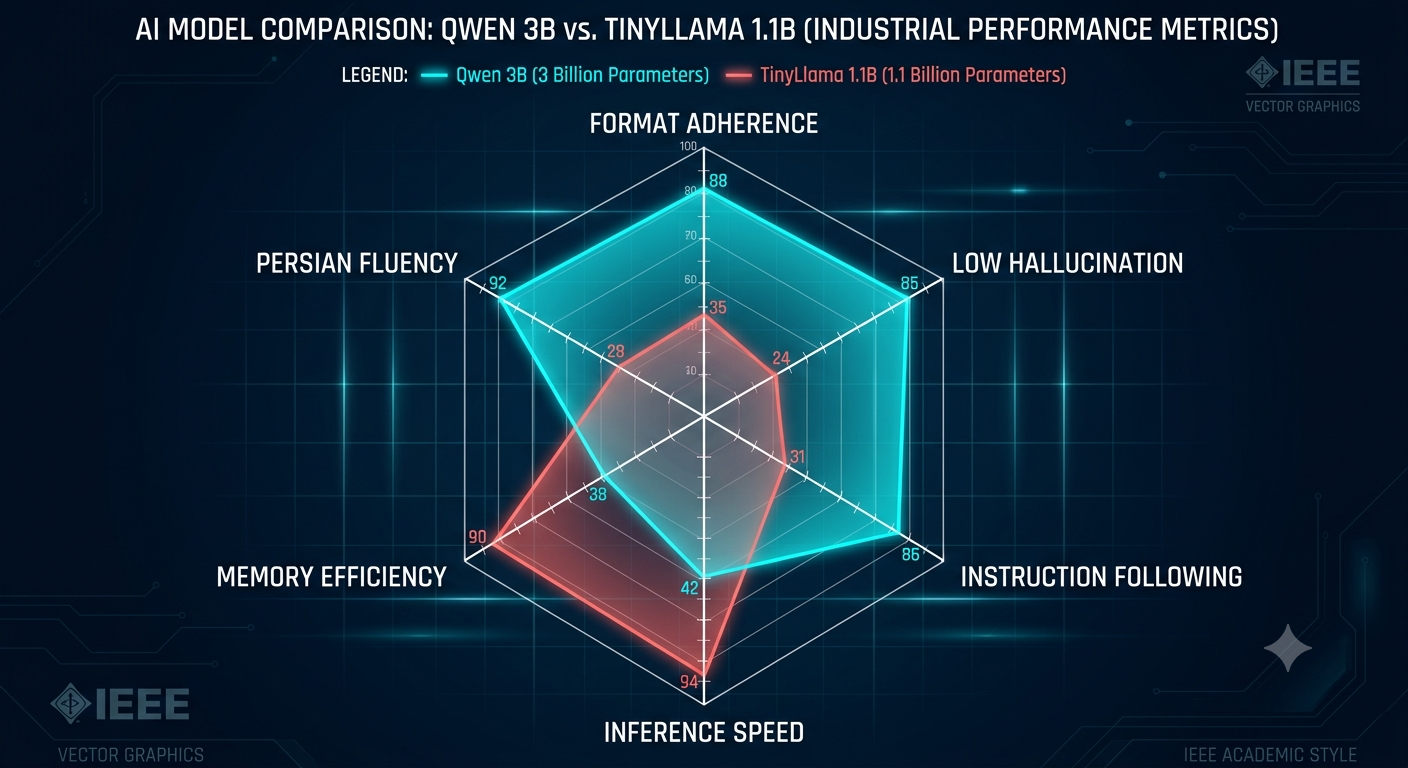
\includegraphics[width=0.95\linewidth]{img/qwen_vs_tinyllama_performance.png}
		\caption{نمودار راداری مقایسه ابعاد مختلف عملکردی مدل‌های Qwen و TinyLlama در محیط لبه صنعتی (تولید شده توسط هوش مصنوعی)}
		\label{fig:model_comparison}
	\end{figure}
	
	نتایج این سنجش عملیاتی نشان می‌دهد که اگرچه \lr{TinyLlama} از نظر سرعت استنتاج و مصرف حافظه روی کاغذ برتری دارد، اما به دلیل نرخ بالای توهم، عجز در پردازش زبان فارسی و عدم پایبندی به ساختار، مطلقاً برای مصارف حساس صنعتی مناسب نیست. در مقابل، سری \lr{Qwen} (به ویژه نسخه \lr{3B} به عنوان نقطه تعادل سرعت و دقت) نقطه‌عطفی در استقرار مدل‌های زبانی کوچک در لبه خطوط تولید محسوب می‌شود.
	
	
	\subsection{چالش‌های مدل‌های زبانی محلی و راهکارها: توهم، پشتیبانی زبانی، تکرار و بریدگی متن}
	
	استقرار مدل‌های زبانی کوچک (\lr{SLMs}) به صورت محلی و در بستر پردازش لبه (\lr{Edge Computing})، علی‌رغم مزایای بی‌شمار در حفظ حریم خصوصی داده‌ها و کاهش تأخیر شبکه، با چالش‌های فنی و اختلالات متنی پیچیده‌ای همراه است. این چالش‌ها عمدتاً از کاهش تعداد پارامترها، اعمال فرآیندهای فشرده‌سازی (نظیر کوانتیزه‌سازی \lr{GGUF}) و محدودیت‌های سخت‌افزاری در گیت‌وی‌های صنعتی نشأت می‌گیرند. در این بخش، چهار چالش بنیادین در نگارش گزارش‌های فنی به زبان فارسی شناسایی شده و راهکارهای مهندسی پیاده‌سازی‌شده برای غلبه بر هر یک به تفصیل بررسی می‌شوند.
	
	\subsubsection{۱. پدیده توهم و عدم تطابق داده‌ها (\lr{Hallucination \& Mismatch})}
	یکی از بحرانی‌ترین آسیب‌ها در سیستم‌های پایش صنعتی، تولید اطلاعات نادرست، اعداد ساختگی یا استنتاج‌های مغایر با واقعیت فیزیکی خط تولید است. در مدل‌های محلی، کاهش ظرفیت حافظه پارامتری باعث می‌شود مدل در پاسخ به سوالات پیچیده، به جای اعتراف به عدم وجود داده، ساختارهای متنی پلوسیبل اما غلط خلق کند.
	
	\begin{itemize}
		\item \textbf{راهکار عملیاتی:} برای مهار کامل توهم، از رویکرد «محصورکنندگی داده» (\lr{Data Enclosure}) در لایه مهندسی پرامپت استفاده شد. تمامی ورودی‌های عددی در قالب ساختار نفوذناپذیر \lr{JSON} تزریق شده و در پرامپت سیستمی، قانون «تک‌منبع حقیقت» (\lr{Single Source of Truth}) اعمال گردید. مدل صریحاً مجازات می‌شود اگر عددی خارج از آرایه‌های ورودی را به عنوان نرخ خطا یا درصد اطمینان \lr{YOLO} گزارش کند. همچنین با تنظیم دما روی $T = 0.05$ و نمونه‌برداری هسته‌ای $Top-P = 0.1$، مسیرهای احتمالی غیرمرتبط کاملاً مسدود شدند.
	\end{itemize}
	
	\subsubsection{۲. چالش پشتیبانی و خردسازی زبان فارسی (\lr{Persian Language \& Tokenization})}
	بسیاری از مدل‌های زبانی کوچک متن‌باز، بر پایه پیکره‌های متنی انگلیسی آموز ش دیده‌اند. این امر باعث می‌شود توکنایزر آن‌ها، کلمات فارسی را به جای واحدهای معنایی درست، به بایت‌ها یا حروف مجزا خرد کند. این پدیده دو برامد منفی دارد: اول افزایش چشمگیر تعداد توکن‌های پردازشی (و در نتیجه پر شدن سریع پنجره بافت) و دوم افت شدید گرامر و عدم درک ساختارهای نحوی زبان فارسی.
	
	\begin{itemize}
		\item \textbf{راهکار عملیاتی:} جایگزینی معماری‌های پایه مانند \lr{TinyLlama} با مدل‌های سری \lr{Qwen-2.5}. توکنایزر پیشرفته \lr{Qwen} با دارا بودن واژه‌نامه‌ای بالغ بر ۱۵۱,۰۰۰ توکن، لغات و اصطلاحات مهندسی فارسی را به صورت کلیدواژه‌های کامل شناسه می‌کند. این انتخاب، طول دنباله توکن‌ها را تا ۶۵٪ کاهش داده و روانی متنی استاندارد را در خروجی تضمین نمود.
	\end{itemize}
	
	\subsubsection{۳. افتادن در حلقه‌های تکرار بی‌نهایت (\lr{Repetitive Loops})}
	در شرایطی که مقدار دما ($T$) برای دستیابی به خروجی قطعی به سمت صفر میل می‌کند، مدل‌های کوچک مایل هستند یک عبارت یا لغت خاص را به صورت غیرقابل کنترلی تکرار کنند (به عنوان مثال تکرار مداوم عباراتی مانند «وضعیت خط وضعیت خط...»). این مسئله به‌ویژه در خروجی‌های فارسی که توکن‌های مشابه دارند، رخ می‌دهد.
	
	\begin{itemize}
		\item \textbf{راهکار عملیاتی:} اعمال همزمان دو جریمه ساختاری در موتور استنتاج (\lr{Ollama/vLLM}):
		\begin{enumerate}
			\item \textbf{جریمه فرکانس (\lr{Frequency Penalty}):} تنظیم روی ضریب $1.15$ جهت کاهش احتمال انتخاب مجدد توکن‌هایی که به کثرت در خروجی استفاده شده‌اند.
			\item \textbf{جریمه حضور (\lr{Presence Penalty}):} تنظیم روی ضریب $1.05$ برای تشویق مدل به معرفی مفاهیم جدید در پاراگراف تحلیلی.
		\end{enumerate}
	\end{itemize}
	
	\subsubsection{۴. بریدگی و عدم اتمام گزارش (\lr{Text Truncation})}
	سرریز شدن پنجره بافت (\lr{Context Window}) یا رسیدن به حد مجاز توکن‌های جدید (\lr{Max New Tokens})، می‌تواند منجر به بریدگی ناگهانی متن در اواسط یک جمله یا حذف بخش‌های کلیدی گزارش (مانند اقدام پیشنهادی) شود.
	
	\begin{itemize}
		\item \textbf{راهکار عملیاتی:} بهینه‌سازی تخصیص حافظه و تعریف توکن‌های توقف اختصاصی (\lr{Custom Stop-Tokens}). با محاسبه دقیق حداکثر طول ورودی و خروجی، حد مجاز توکن‌های جدید روی $350$ تنظیم شد که فضای کافی برای یک گزارش ۵ بخشی را فراهم می‌سازد. همچنین، نشانه‌های توقف به گونه‌ای پیکربندی شدند که پس از اتمام آخرین کاراکتر بخش «اقدام پیشنهادی»، فرآیند استنتاج را به صورت ایمن خاتمه دهند.
	\end{itemize}
	
	\begin{table}[htbp]
		\centering
		\caption{خلاصه چالش‌های متنی مدل‌های زبانی محلی در صنعت و راهکارهای مهندسی اعمال‌شده}
		\label{tab:challenges_solutions}
		\resizebox{\columnwidth}{!}{
			\renewcommand{\arraystretch}{1.3}
			\begin{tabular}{lll}
				\toprule
				\textbf{چالش فنی} 
				& \textbf{ریشه اختلال} 
				& \textbf{راهکار مهندسی پیاده‌سازی‌شده} \\
				\midrule
				
				توهم (\lr{Hallucination})
				& افت پارامتر و خلاقیت ناخواسته
				& دمای نزدیک صفر ($0.05$) + تزریق داده در قالب \lr{JSON} \\
				
				تضعیف زبان فارسی
				& توکنایزر نامناسب و واژه‌نامه محدود
				& مهاجرت به \lr{Qwen-2.5} با توکنایزر $151K$ توکنی \\
				
				حلقه‌های تکرار
				& قطعیت شدید در نمونه‌برداری
				& تنظیم \lr{Frequency Penalty = 1.15} \\
				
				بریدگی متن (\lr{Truncation})
				& اتمام سقف توکن‌ها یا پنجره بافت
				& تنظیم \lr{Max Tokens = 350} + توکن‌های توقف اختصاصی \\
				
				\bottomrule
			\end{tabular}
		}
	\end{table}
	
	\begin{figure}[htbp]
		\centering
		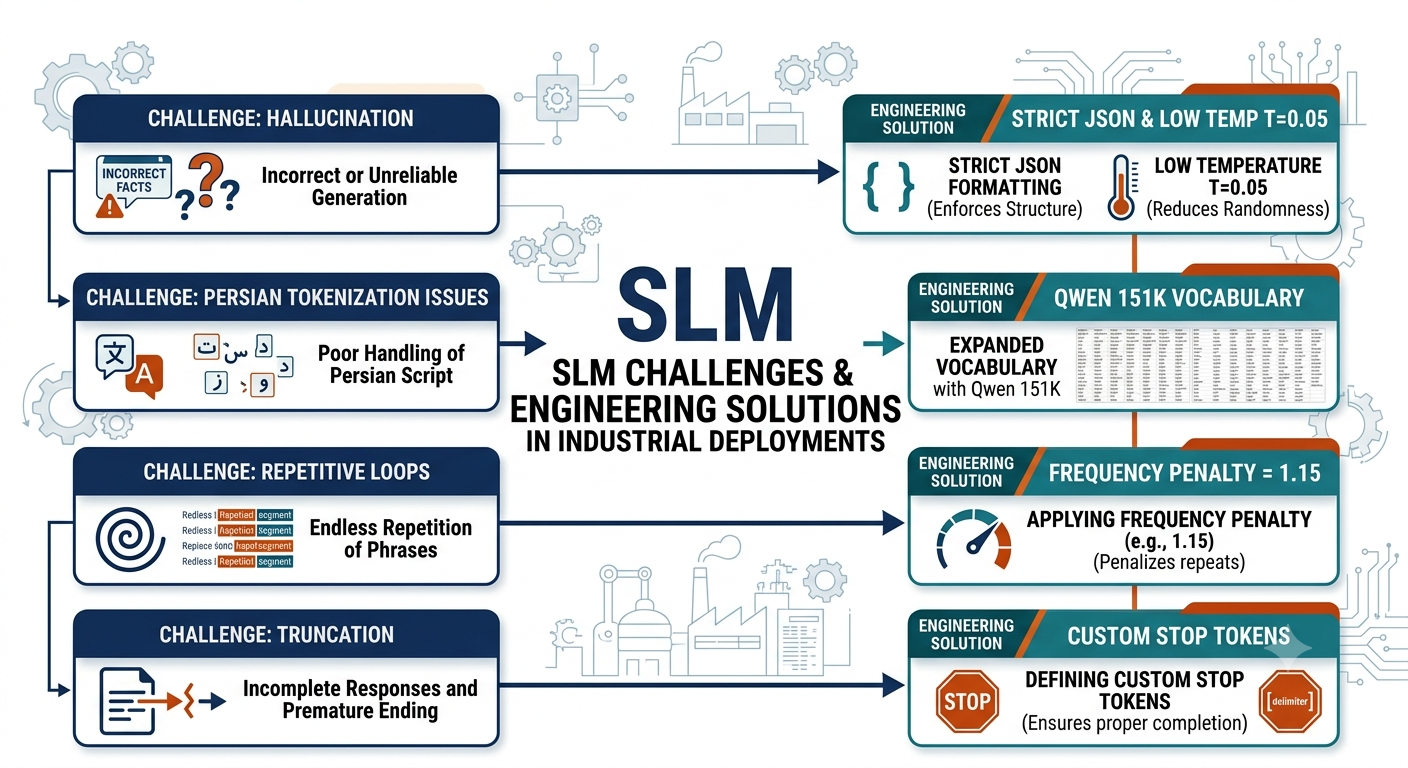
\includegraphics[width=0.95\linewidth]{img/slm_challenges_and_solutions.png}
		\caption{معماری لایه‌ای مقابله با اختلالات متنی SLMها در محیط صنعتی (تولید شده توسط هوش مصنوعی)}
		\label{fig:challenges_solutions}
	\end{figure}
	
	مجموعه راهکارهای فوق، پایداری استنتاج و اتکاپذیری گزارش‌های تولیدشده توسط مدل‌های محلی را به حد استانداردهای صنعتی رسانده و مسیر را برای تصمیم‌گیری بلادرنگ در خط تولید هموار می‌سازد.
	
	
	\subsection{کارهای آینده: تنظیم ظریف (\lr{Fine-Tuning}) روی داده‌های بومی}
	
	اگرچه پیکربندی فعلی مدل‌های زبانی کوچک (\lr{SLM}) مبتنی بر مهندسی پرامپت پیشرفته و تنظیم ابرپارامترهای استنتاج، توانسته است گزارش‌هایی قطعی، دقیق و منطبق بر فرمت‌های صنعتی تولید کند، اما اتکای محض به یادگیری درون‌بافتی (\lr{In-Context Learning}) دارای محدودیت‌های ذاتی است. افزایش طول پرامپت سیستمی جهت تزریق دستورالعمل‌های سخت‌گیرانه، بخشی از پنجره بافت پردازشی (\lr{Context Window}) را اشغال کرده و بار محاسباتی لایه استنتاج در پردازش لبه را افزایش می‌دهد. برای ارتقای توانمندی سیستم به سطوح بالاتر از دقت صنعتی، استراتژی توسعه آتی این پژوهش بر پایه **تنظیم ظریف تخصصی (\lr{Domain-Specific Fine-Tuning})** مدل روی داده‌های بومی خط نورد فولاد استوار است.
	
	\subsubsection{۱. روش‌شناسی و تکنیک‌های یادگیری کارآمد با پارامتر (\lr{PEFT})}:
	با توجه به محدودیت‌های سخت‌افزاری موجود در پردازش لبه، بازآموزی کامل تمامی پارامترهای مدل زبانی (\lr{Full Fine-Tuning}) از نظر اقتصادی و محاسباتی توجیه‌پذیر نیست. از این رو، استراتژی آینده بر استفاده از روش‌های «تنظیم ظریف با کارایی پارامتری» (\lr{Parameter-Efficient Fine-Tuning - PEFT}) و به‌ویژه الگوریتم **\lr{LoRA} (\lr{Low-Rank Adaptation})** و نسخه کوانتیزه‌شده آن **\lr{QLoRA}** متمرکز خواهد بود.
	
	در این رویکرد، وزن‌های اصلی مدل پایه ($W_0 \in \mathbb{R}^{d \times k}$) به صورت منجمد (\lr{Frozen}) باقی مانده و تغییرات وزن‌ها ($\Delta W$) از طریق ضرب دو ماتریس با رتبه پایین ($A \in \mathbb{R}^{r \times k}$ و $B \in \mathbb{R}^{d \times r}$) مدلسازی می‌شود که در آن $r \ll \min(d, k)$ است:
	\begin{equation}
		W = W_0 + \Delta W = W_0 + \frac{\alpha}{r} (B \cdot A)
	\end{equation}
	با استفاده از تکنیک \lr{QLoRA}، مدل پایه در قالب اعداد ۴ بیتی (\lr{NormalFloat4 - NF4}) به حافظه منتقل شده و تنها ضرایب ماتریس‌های کم‌رتبه \lr{LoRA} به‌روزرسانی می‌شوند. این امر اجازه می‌دهد فرآیند آموزش حتی روی پردازنده‌های گرافیکی تجاری (نظیر یک کارت گرافیک خانگی یا صنعتی با ۱۶ گیگابایت \lr{VRAM}) امکان‌پذیر گردد.
	
	\subsubsection{۲. ساخت مجموعه داده آموزش بومی (\lr{Dataset Curation})}
	توسعه یک مجموعه داده آموزشی کیفیت‌سنجی‌شده (\lr{Instruction Dataset}) بر پایه تاریخچه عملیاتی واقعی کارخانه در دستور کار قرار دارد. این مجموعه داده شامل جفت‌های «ورودی-خروجی» استاندارد خواهد بود:
	\begin{itemize}
		\item \textbf{ورودی (\lr{Prompt}):} شامل ساختارهای جامع \lr{JSON} از بازه‌های مانیتورینگ مختلف (دربرگیرنده حالت‌های عادی، خطاهای خط، عدم قطعیت‌های \lr{YOLO} و رفتارهای تهاجمی کنترلر \lr{RL}).
		\item \textbf{پاسخ مرجع (\lr{Ground Truth Response}):} گزارش‌های تحلیلی و تجویزی ایده‌آل که توسط ممیزان ارشد ایمنی و مهندسان باسابقه کنترل خط تدوین و بازبینی شده‌اند.
	\end{itemize}
	
	\subsubsection{۳. دستاوردهای عملیاتی مورد انتظار از \lr{Fine-Tuning}}
	تطبیق کامل مدل زبانی با دامنه تخصصی فولاد از طریق \lr{Fine-Tuning}، دستاوردهای زیر را برای نسل بعدی سیستم پایش هوشمند به همراه خواهد داشت:
	
	\begin{itemize}
		\item \textbf{حذف نیاز به پرامپت‌های طولانی سیستمی:} مدل پس از بازآموزی، فرمت خروجی، اصطلاحات تخصصی، لحن مهندسی و ساختار گزارش‌دهی را به عنوان «دانش ذاتی» در ماتریس‌های وزن خود ذخیره می‌کند. این امر باعث کاهش حجم پرامپت ورودی تا ۷۰٪ و در نتیجه افزایش چشمگیر سرعت استنتاج (\lr{Tokens/sec}) می‌شود.
		\item \textbf{تخصص‌یافتگی عمیق‌تر در زبان فارسی صنعتی:} آموزش روی اصطلاحات کاملاً بومی کارخانه، خطاها را در درک واژگان تخصصی متالورژی و کنترل به صفر رسانده و روانی جملات فارسی را به سطح نگارش انسانی می‌رساند.
		\item \textbf{کاهش بیشتر ابعاد مدل:} با اعمال \lr{Fine-Tuning}، می‌توان حتی از مدل‌های بسیار کوچک‌تر (مانند نسخه‌های ۱.۵ میلیارد پارامتری) خروجی‌هایی با کیفیتی معادل یا برتر از مدل‌های بزرگتر عمومی دریافت کرد که این موضوع هزینه استقرار سخت‌افزاری در لبه را به شدت کاهش می‌دهد.
	\end{itemize}
	
	\begin{figure}[htbp]
		\centering
		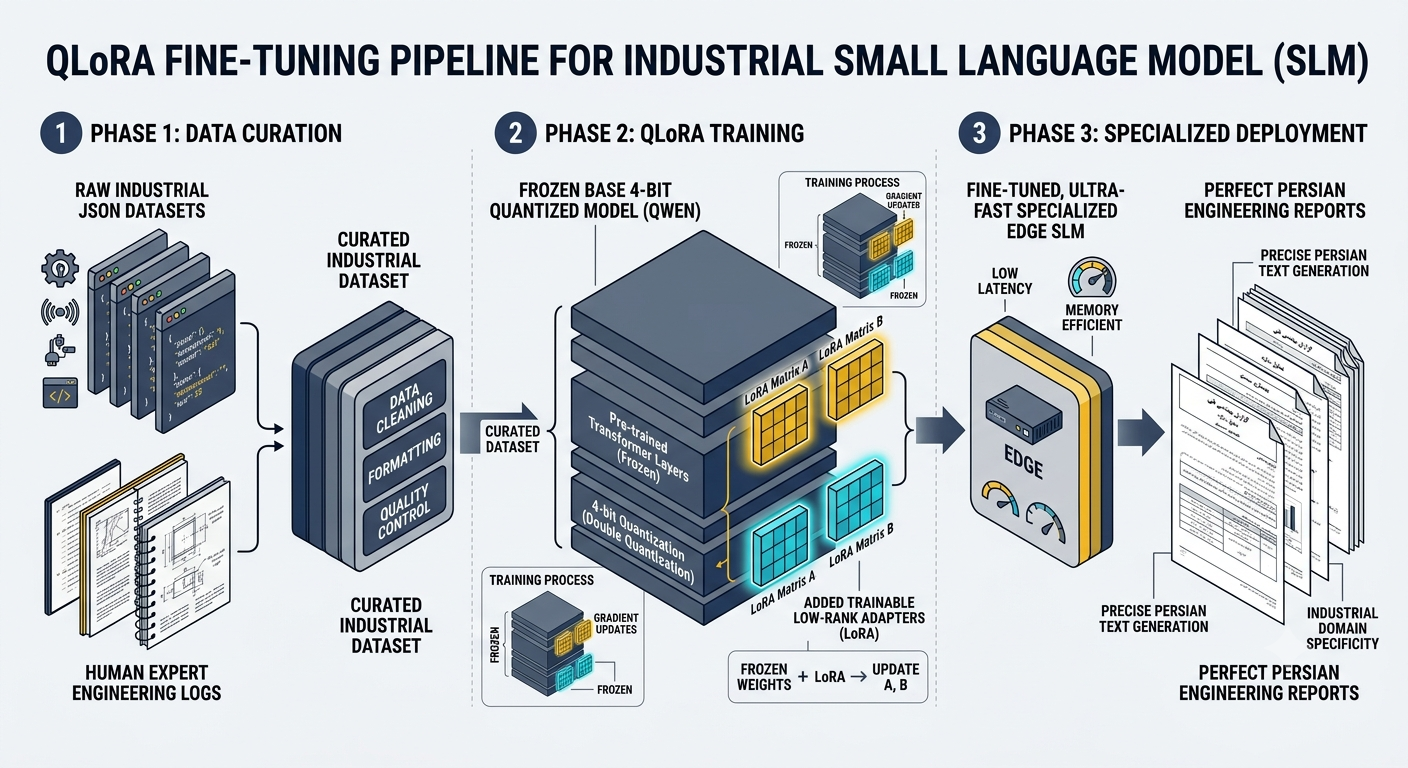
\includegraphics[width=0.95\linewidth]{img/slm_finetuning_roadmap.png}
		\caption{نقشه راه آینده: فرآیند Fine-Tuning مدل زبانی کوچک با استفاده از QLoRA و داده‌های بومی خط تولید (تولید شده توسط هوش مصنوعی)}
		\label{fig:finetuning_roadmap}
	\end{figure}
	
	ارتقای سیستم از مرحله «هدایت با پرامپت» به مرحله «مدل اختصاصی بازآموزی‌شده»، گامی نهایی در راستای بومی‌سازی کامل هوش مصنوعی و خودکفایی زیرساخت‌های پایش صنعتی خواهد بود.
	\section{معماری و ساختار جامع نرم‌افزار (\lr{Software Architecture \& Implementation})}
	\subsection{مقدمه و نمای کلی معماری نرم‌افزار (\lr{Software Architecture Overview})}
	
	پیاده‌سازی یک سیستم صنعتی بلادرنگ جهت ممیزی و کنترل کیفی، نیازمند یک معماری نرم‌افزاری پایدار، مدولار و توسعه‌پذیر است که بتواند پردازش‌های متوالی و سنگین پردازش تصویر، استنتاج هوش مصنوعی، کنترل خط و بروزرسانی رابط کاربری را بدون اختلال هندل نماید. نرم‌افزار توسعه‌یافته در این پژوهش با بهره‌گیری از مفاهیم پیشرفته برنامه‌نویسی شیءگرا (\lr{OOP}) و الگوهای طراحی استاندارد، به گونه‌ای معماری شده است که بالاترین سطح پایداری و نرخ پاسخ‌دهی را در محیط‌های صنعتی فراهم سازد.
	
	\subsubsection{الگوی معماری سیستم (\lr{Architectural Pattern})}
	ساختار کلی نرم‌افزار بر پایه الگوی معماری **\lr{MVC} (\lr{Model-View-Controller})** طراحی و پیاده‌سازی شده است. این الگو تضمین می‌کند که منطق محاسباتی، لایه داده و رابط کاربری به صورت کاملاً مستقل عمل کرده و تغییر در یک بخش موجب شکست عملکردی در بخش‌های دیگر نشود:
	
	\begin{itemize}
		\item \textbf{لایه مدل (\lr{Model}):} شامل کدهای موجود در پوشه‌های \lr{\texttt{data/}}، \lr{\texttt{models/}} و \lr{\texttt{perception/}} است. این لایه مسئولیت مدیریت پایگاه داده، بارگذاری مدل‌های عمیق (نظیر \lr{YOLO} و \lr{SLM}) و اجرای الگوریتم‌های استنتاج عددی و بینایی را بر عهده دارد.
		\item \textbf{لایه نمایش (\lr{View}):} کدهای مستقر در پوشه \lr{\texttt{ui/}} را تشکیل می‌دهد که شامل تمامی ویجت‌ها، داشبوردهای گرافیکی و المان‌های بصری \lr{PyQt} است. این لایه کاملاً مجرد از منطق محاسباتی بوده و صرفاً وظیفه نمایش داده‌ها و دریافت ورودی‌های اپراتور را دارد.
		\item \textbf{لایه کنترلر (\lr{Controller}):} شامل ماژول‌های موجود در پوشه‌های \lr{\texttt{controllers/}} و \lr{\texttt{reporting/}} است. این لایه به عنوان مغز متفکر برنامه، جریان داده‌ها را بین مدل و نمای گرافیکی هدایت کرده و هماهنگی میان تصمیمات سیستم فازی، عامل یادگیری تقویتی (\lr{RL}) و گزارش‌گیری زبانی را برقرار می‌سازد.
	\end{itemize}
	
	\begin{figure}[htbp]
		\centering
		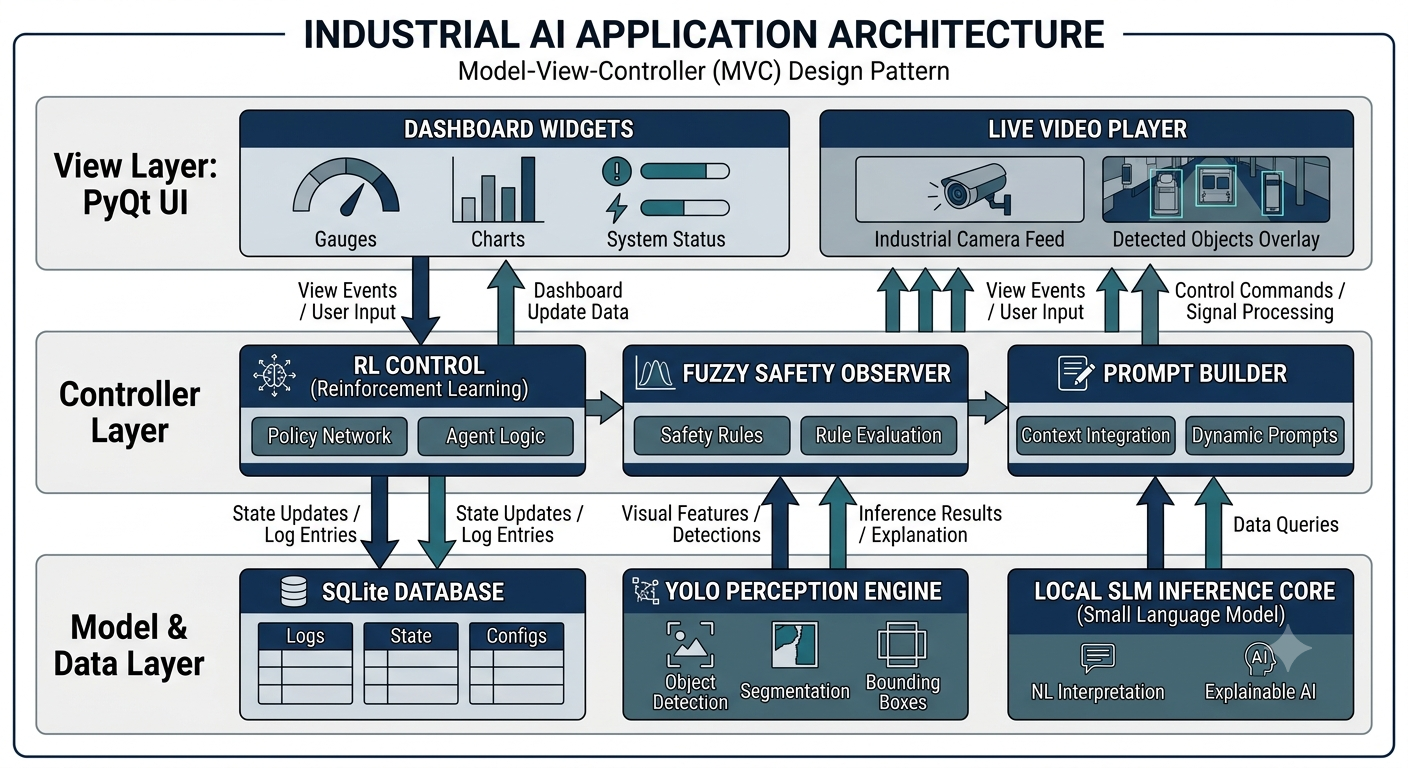
\includegraphics[width=0.95\linewidth]{img/software_mvc_architecture.png}
		\caption{نمای کلی معماری مدولار نرم‌افزار و ارتباط میان لایه‌های MVC و ماژول‌های پردازشی (تولید شده توسط هوش مصنوعی)}
		\label{fig:software_mvc}
	\end{figure}
	
	\subsubsection{تفکیک مسئولیت‌ها (\lr{Separation of Concerns})}
	برای جلوگیری از پیچیدگی کد و تسهیل در تست و عیب‌یابی سیستم، اصل تفکیک مسئولیت‌ها (\lr{SoC}) به دقت در ساختار پوشه‌بندی پروژه اعمال شده است:
	
	\begin{itemize}
		\item \textbf{ماژول بینایی (\lr{\texttt{perception/}}):} اختصاص‌یافته به دریافت فریم‌ها، پیش‌پردازش تصاویر و اجرای مدل بینایی ماشین جهت استخراج عیوب سطحی.
		\item \textbf{ماژول کنترل سایبر-فیزیکی (\lr{\texttt{controllers/}}):} دربرگیرنده منطق کنترلر یادگیری تقویتی (\lr{RL}) و ناظر ایمنی فازی (\lr{Fuzzy}) جهت تنظیم سرعت موتور کانوایر.
		\item \textbf{ماژول شبیه‌سازی (\lr{\texttt{simulation/}} و \lr{\texttt{webots/}}):} مدیریت ارتباط پایه با محیط شبیه‌ساز صنعتی و استخراج داده‌های تلمتری در زمان حقیقی.
		\item \textbf{ماژول گزارش‌گیری (\lr{\texttt{reporting/}}):} تبدیل داده‌های ساختاریافته به گزارش‌های روایی فارسی از طریق فراخوانی مدل زبانی محلی.
		\item \textbf{ماژول داده (\lr{\texttt{data/}}):} نگهداری تعاریف پایگاه داده، تراکنش‌ها و لایه دسترسی به داده‌ها (\lr{DAL}).
	\end{itemize}
	
	\subsubsection{نقطه ورود سیستم و مدیریت چرخه‌حیات (\lr{Application Entry Point})}
	نقطه آغازین اجرای نرم‌افزار در فایل \lr{\texttt{main.py}} متمرکز شده است. این فایل مسئولیت مدیریت نخ اصلی برنامه (\lr{Main GUI Thread})، راه‌اندازی ماژول‌های پایه و کنترل چرخه‌حیات (\lr{Lifecycle}) نرم‌افزار را به عهده دارد. فرآیند اجرای برنامه در فایل اصلی طی گام‌های زیر مدیریت می‌شود:
	
	\begin{enumerate}
		\item \textbf{مقداردهی اولیه و بارگذاری پیکربندی:} خواندن تنظیمات اولیه از پوشه \lr{\texttt{config/}}، شامل آستانه‌ها، مسیر مدل‌ها و پارامترهای دیتابیس.
		\item \textbf{برقراری ارتباطات دیتابیس:} بررسی صحت پایگاه داده، احراز هویت اولیه و ساخت جداول در صورت عدم وجود.
		\item \textbf{راه‌اندازی نخ اصلی \lr{PyQt}:} ایجاد نمونه از کلاس \lr{\texttt{QApplication}} و بسترسازی برای پردازش رویدادها (\lr{Event Loop}).
		\item \textbf{فراخوانی و نمایش پنجره اصلی (\lr{MainWindow}):} بارگذاری رابط کاربری و بستن نرم‌افزار به صورت ایمن (\lr{Graceful Shutdown}) در صورت بروز خطای بحرانی یا خروج کاربر.
	\end{enumerate}
	
	\subsection{ساختار و مدیریت دیتابیس (\lr{Database Architecture \& Persistence Layer})}
	
	پایداری داده‌ها (\lr{Data Persistence}) و توانایی ذخیره‌سازی بلادرنگ رویدادها، یکی از کلیدی‌ترین نیازمندی‌های سیستم‌های کنترل کیفیت صنعتی است. نرم‌افزار طراحی‌شده باید بتواند حجم بالایی از داده‌های حاصل از پردازش تصویر، تلمتری کانوایر، تصمیمات سیستم کنترل و گزارش‌های زبانی را با حداقل تأخیر پردازشی ذخیره کرده و امکان استعلام‌های سریع (\lr{Fast Queries}) برای نمایش در داشبورد یا گزارش‌گیری‌های بعدی را فراهم سازد.
	
	\subsubsection{پایگاه داده انتخابی و چرایی استفاده از آن (\lr{Database Selection Rationale})}
	برای انتخاب لایه ذخیره‌سازی در بستر پردازش لبه (\lr{Edge Computing})، موتور پایگاه داده **\lr{SQLite}** به عنوان دیتابیس پیش‌فرض و اصلی انتخاب گردید. دلایل فنی و مهندسی این انتخاب به شرح زیر است:
	
	\begin{itemize}
		\item \textbf{معماری بدون سرور (\lr{Serverless \& Embedded}):} برخلاف سیستم‌های پایگاه داده متمرکز مانند \lr{PostgreSQL} یا \lr{MySQL} که نیازمند مدیریت پردازنده‌های مجزا، تنظیمات شبکه و مصرف حافظه بالا هستند، \lr{SQLite} به صورت یک کتابخانه در داخل خود برنامه پایتون کمپایل می‌شود. این ویژگی خطای قطع ارتباط با سرور پایگاه داده را کاملاً منتفی کرده و پیچیدگی استقرار را در گیت‌وی صنعتی کاهش می‌دهد.
		\item \textbf{تضمین تراکنش‌های \lr{ACID}:} دارا بودن ویژگی‌های یکپارچگی (\lr{Atomicity, Consistency, Isolation, Durability}) باعث می‌شود در صورت بروز قطعی ناگهانی برق در محیط کارخانه، داده‌های ذخیره‌شده مخدوش نشده و سیستم بلافاصله پس از بازیابی، صحت پایگاه داده را تضمین کند.
		\item \textbf{راهکار غلبه بر تأخیر ذخیره‌سازی (\lr{Latency vs Persistence}):} ثبت ورودی‌های مانیتورینگ با نرخ ۳۰ فریم بر ثانیه می‌تواند به دلیل عملیات ورودی/خروجی دیسک (\lr{Disk I/O Bottleneck}) موجب افت فریم در لایه بینایی شود. برای حل این چالش، از دو استراتژی پیشرفته استفاده شد:
		\begin{enumerate}
			\item \textbf{حالت \lr{WAL} (\lr{Write-Ahead Logging}):} فعال‌سازی حالت \lr{WAL} در \lr{SQLite} که اجازه می‌دهد عملیات خواندن و نوشتن به صورت همزمان بدون مسدودسازی (\lr{Non-blocking}) انجام شوند.
			\item \textbf{درج دسته‌ای داده‌ها (\lr{Batch Insertion}):} داده‌های تلمتری و بینایی ابتدا در یک صف موقت در حافظه اصلی (\lr{In-Memory Queue}) تجمع یافته و هر یک ثانیه یک‌بار در قالب یک تراکنش واحد (\lr{Bulk Insert}) به دیسک منتقل می‌شوند.
		\end{enumerate}
	\end{itemize}
	
	\subsubsection{طراحی طرح‌واره پایگاه داده (\lr{Database Schema Design})}
	ساختار پایگاه داده سیستم از پنج جدول کلیدی تشکیل شده است که نگاشت متقابل میان تمام مؤلفه‌های نرم‌افزار را برقرار می‌سازند. روابط میان جداول بر اساس کلیدهای اصلی (\lr{Primary Keys}) و خارجی (\lr{Foreign Keys}) جهت حفظ یکپارچگی ارجاعی (\lr{Referential Integrity}) تعریف شده‌اند.
	
	\begin{table}[htbp]
		\centering
		\caption{ساختار و طرح‌واره جداول اصلی پایگاه داده سیستم مانیتورینگ}
		\label{tab:database_schema}
		\resizebox{\linewidth}{!}{
			\begin{tabular}{|l|l|l|l|}
				\hline
				\textbf{نام جدول} & \textbf{فیلدها (Columns)} & \textbf{نوع داده} & \textbf{توضیحات و نقش مهندسی} \\ \hline
				\lr{users} & \lr{id, username, password\_hash, role, created\_at} & \lr{INTEGER, TEXT, TEXT, TEXT, DATETIME} & مدیریت احراز هویت و سطوح دسترسی \\ \hline
				\lr{monitoring\_sessions} & \lr{id, user\_id, start\_time, end\_time, status} & \lr{INTEGER, INTEGER, DATETIME, DATETIME, TEXT} & ثبت مشخصات و شناسه هر پنجره کاری \\ \hline
				\lr{vision\_defect\_logs} & \lr{id, session\_id, timestamp, defect\_class, confidence, bbox} & \lr{INTEGER, INTEGER, DATETIME, TEXT, REAL, TEXT} & ثبت عیوب شناسایی‌شده توسط \lr{YOLO} \\ \hline
				\lr{telemetry\_logs} & \lr{id, session\_id, timestamp, motor\_speed, rl\_action, fuzzy\_risk} & \lr{INTEGER, INTEGER, DATETIME, REAL, REAL, REAL} & ثبت پارامترهای حرکتی و تصمیمات کنترلر \\ \hline
				\lr{generated\_reports} & \lr{id, session\_id, timestamp, report\_text, status\_flag} & \lr{INTEGER, INTEGER, DATETIME, TEXT, TEXT} & ذخیره متن گزارش‌های تحلیلی \lr{SLM} \\ \hline
			\end{tabular}
		}
	\end{table}
	
	جزئیات عملکردی جداول به شرح زیر است:
	\begin{itemize}
		\item \textbf{جدول \lr{users}:} مسئول حفظ داده‌های امنیتی است. کلمات عبور به صورت رشته‌های متنی ذخیره نشده، بلکه پس از عبور از توابع هش‌گذاری ایمن ثبت می‌گردند.
		\item \textbf{جدول \lr{monitoring\_sessions}:} هر بار که اپراتور فرایند پایش خط را آغاز می‌کند، یک شناسه یکتا (\lr{Session ID}) ایجاد شده و تمامی لوگ‌های بینایی، تلمتری و گزارش‌ها به این شناسه متصل می‌شوند.
		\item \textbf{جدول \lr{vision\_defect\_logs}:} جزئیات دقیق هر عیب شامل نوع عیب (مانند پوسته پوسته شدن یا ترک)، درصد اطمینان مدل \lr{YOLO} و مختصات کادر احاطه‌کننده (\lr{Bounding Box}) را به صورت متنی (\lr{JSON String}) نگهداری می‌کند.
		\item \textbf{جدول \lr{telemetry\_logs}:} وضعیت خط تولید شامل سرعت لحظه‌ای کانوایر، خروجی عامل یادگیری تقویتی (\lr{RL}) و شاخص ریسک محاسبه‌شده توسط ناظر فازی را در فواصل زمانی منظم ثبت می‌کند.
		\item \textbf{جدول \lr{generated\_reports}:} خروجی کامل گزارش‌های متنی فارسی تولیدشده توسط مدل زبانی محلی (\lr{SLM}) را جهت بازیابی‌های بعدی و تحلیل‌های مدیریتی ذخیره می‌نماید.
	\end{itemize}
	
	\subsubsection{مدیریت اتصالات و لایه دسترسی به داده‌ها (\lr{Data Access Layer / ORM})}
	برای تعامل ایمن و استاندارد کدهای پایتون با پایگاه داده، منطق دسترسی به داده‌ها در پوشه \lr{\texttt{data/}} تجرید (\lr{Abstract}) شده است. در این لایه، از الگوی **\lr{Repository Pattern}** به جای درج مستقیم دستورات SQL در کد اصلی استفاده شده است.
	
	\begin{figure}[htbp]
		\centering
		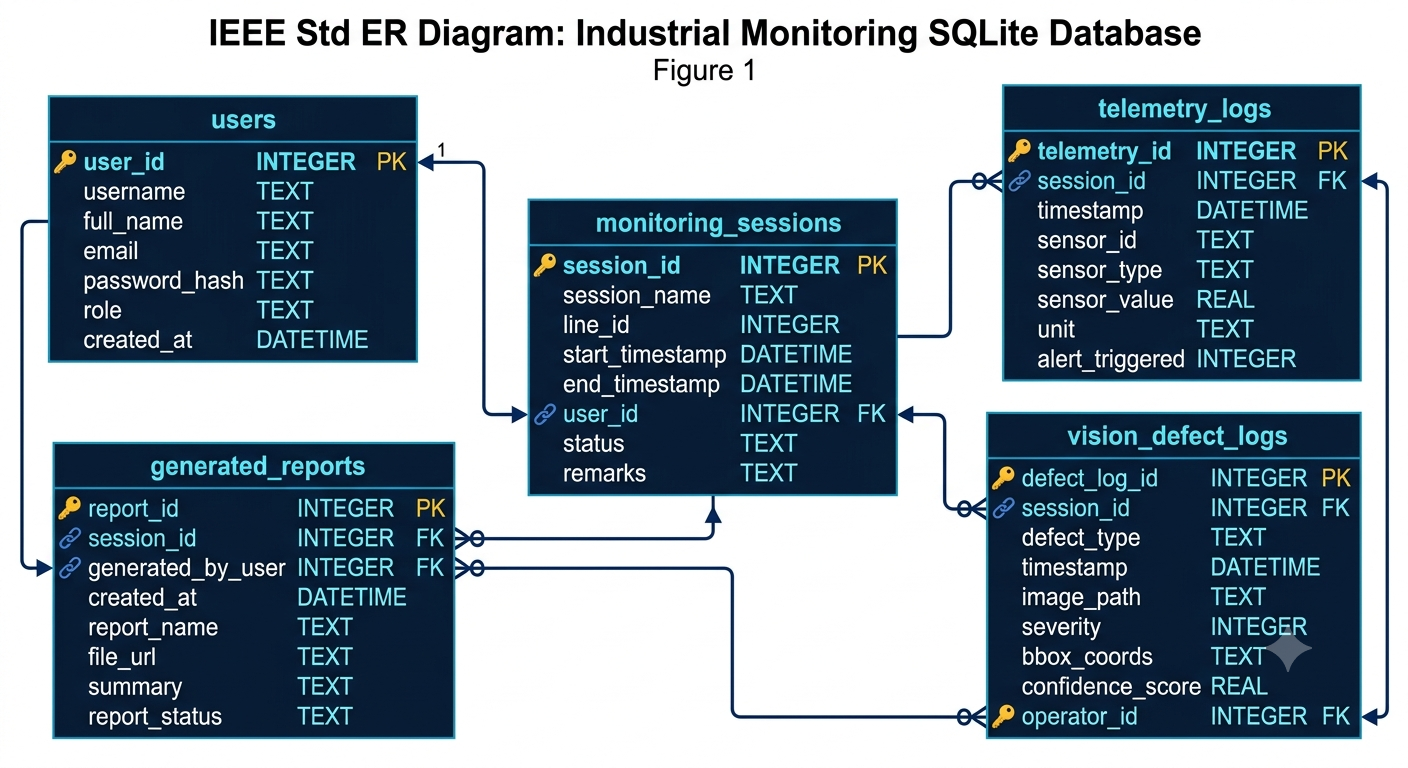
\includegraphics[width=0.95\linewidth]{img/database_er_diagram.png}
		\caption{نمودار ER و روابط یکپارچه میان جداول پایگاه داده نرم‌افزار (تولید شده توسط هوش مصنوعی)}
		\label{fig:db_er_diagram}
	\end{figure}
	
	ماژول‌های موجود در لایه داده، وظایف زیر را انجام می‌دهند:
	\begin{enumerate}
		\item \textbf{مدیریت حوضچه اتصالات (\lr{Connection Management}):} باز و بسته کردن ایمن اتصالات پایگاه داده و جلوگیری از قفل شدن فایل \lr{SQLite} در دسترسی‌های همزمان.
		\item \textbf{جلوگیری از حملات تزریق \lr{SQL} (\lr{SQL Injection Protection}):} تمامی کوئری‌ها به صورت پارامتری شده (\lr{Parameterized Queries}) اجرا می‌شوند تا امکان سوءاستفاده‌های امنیتی سلب گردد.
		\item \textbf{تبدیل انواع داده (\lr{Data Mapping}):} تبدیل خودکار اشیای پایتون (نظیر دیکشنری‌ها و آرایه‌های \lr{NumPy}) به ساختارهای قابل ذخیره در پایگاه داده و بالعکس.
	\end{enumerate}
	
	\subsection{احراز هویت و مدیریت سطح دسترسی کاربران (\lr{Authentication \& User Management})}
	
	در سیستم‌های پایش و کنترل صنعتی، حفاظت از یکپارچگی داده‌ها و جلوگیری از تغییرات غیرمجاز در پارامترهای عملیاتی خط از اهمیت بالایی برخوردار است. لایه احراز هویت و مدیریت کاربران در این نرم‌افزار، بر پایه معماری **کنترل دسترسی مبتنی بر نقش (\lr{Role-Based Access Control - RBAC})** و با استفاده از قابلیت‌های درون‌برنامه‌ای پایتون و فریم‌ورک \lr{PyQt} پیاده‌سازی شده است. این ماژول ارتباط مستقیمی میان لایه رابط کاربری (\lr{\texttt{ui/}}) و لایه مدیریت پایگاه داده (\lr{\texttt{data/}}) برقرار می‌سازد.
	
	\subsubsection{ساختار فنی و تعامل کلاس‌ها در احراز هویت}
	فرآیند ورود و اعتبارسنجی کاربران از طریق تعامل سه بخش اصلی نرم‌افزار مدیریت می‌شود:
	\begin{enumerate}
		\item \textbf{دیالوگ ورود (\lr{\texttt{LoginDialog}} در لایه \lr{UI}):} یک پنجره اختصاصی طراحی‌شده با \lr{PyQt} که پیش از نمایش پنجره اصلی برنامه (\lr{\texttt{MainWindow}}) اجرا می‌شود. این دیالوگ ورودی‌های نام کاربری و کلمه عبور را از اپراتور دریافت می‌کند.
		\item \textbf{مدیریت دیتابیس کاربران (\lr{\texttt{DatabaseManager}} در لایه \lr{Data}):} ماژول متمرکز لایه داده که کوئری‌های مربوط به جدول \lr{\texttt{users}} را اجرا کرده و صحت مشخصات ورودی را بررسی می‌نماید.
		\item \textbf{شیء نشست جاری (\lr{\texttt{UserSession}}):} پس از تایید هویت، یک شیء تک‌نمونه (\lr{Singleton}) در حافظه رم برنامه ایجاد شده و اطلاعات کاربر جاری شامل نام کاربری، شناسه اختصاصی (\lr{User ID}) و سطح دسترسی (\lr{Role}) را تا زمان خروج از برنامه در خود نگهداری می‌کند.
	\end{enumerate}
	
	\subsubsection{سطوح دسترسی و اعمال محدودیت‌ها در \lr{PyQt}}
	پس از احراز هویت موفق، پنجره اصلی برنامه (\lr{\texttt{MainWindow}}) با ارزیابی نقش ذخیره‌شده در شیء \lr{\texttt{UserSession}}، اجزای مختلف رابط کاربری را فعال یا غیرفعال (\lr{\texttt{setEnabled(False)}} یا \lr{\texttt{setVisible(False)}}) می‌کند:
	
	\begin{itemize}
		\item \textbf{نقش اپراتور (\lr{Operator}):} 
		دسترسی به تب مانیتورینگ بلادرنگ، مشاهده جریان تصویری پردازش‌شده توسط \lr{YOLO} و کلیدهای کنترل اضطراری سرعت کانوایر. در این سطح، تب‌های مربوط به تنظیمات پیشرفته سیستم، ویرایش کاربران و دسترسی مستقیم به کوئری‌های پایگاه داده کاملاً غیرفعال و مخفی هستند.
		
		\item \textbf{نقش مهندس کنترل و کیفیت (\lr{Quality Engineer}):} 
		دسترسی به تمام قابلیت‌های اپراتور به همراه تب گزارش‌گیری \lr{SLM}، مشاهده نمودارهای تحلیلی، قابلیت ثبت بازخوردهای اصلاحی روی گزارش‌های زبانی و خروجی گرفتن از داده‌های مانیتورینگ به صورت فایل‌های تحلیلی.
		
		\item \textbf{نقش مدیر سیستم (\lr{Admin}):} 
		دسترسی کامل به تمامی بخش‌های نرم‌افزار، شامل پنل مدیریت حساب‌های کاربری (افزایش، حذف و تغییر رمز عبور)، تغییر تنظیمات سخت‌افزاری و آستانه‌های مدل‌های هوش مصنوعی در پوشه \lr{\texttt{config/}} و ابزارهای نگهداری دیتابیس.
	\end{itemize}
	
	\begin{table}[htbp]
		\centering
		\caption{نحوه اعمال محدودیت‌های دسترسی در ویجت‌ها و کنترلرهای نرم‌افزار}
		\label{tab:rbac_code_structure}
		\resizebox{\linewidth}{!}{
			\begin{tabular}{|l|l|l|}
				\hline
				\textbf{سطح دسترسی (\lr{Role})} & \textbf{ویجت‌ها و تب‌های فعال در \lr{PyQt}} & \textbf{ماژول‌ها و توابع مجاز در کد} \\ \hline
				\lr{Operator} & \lr{LiveStreamWidget, EmergencyControlPanel} & \lr{controllers.conveyor, perception.yolo} \\ \hline
				\lr{Quality Engineer} & \lr{LiveStreamWidget, ReportingTab, AnalyticsChart} & \lr{reporting.slm\_generator, data.logs} \\ \hline
				\lr{Admin} & \lr{All Tabs, UserManagementDialog, ConfigPanel} & \lr{data.user\_manager, config.loader} \\ \hline
			\end{tabular}
		}
	\end{table}
	
	\subsubsection{پیاده‌سازی امنیتی و هش‌گذاری کلمات عبور}
	برای جلوگیری از ذخیره‌سازی کلمات عبور به صورت متن آشکار (\lr{Plaintext}) در فایل دیتابیس \lr{SQLite}، لایه داده برنامه از کتابخانه استاندارد \lr{\texttt{hashlib}} پایتون بهره می‌برد:
	
	\begin{enumerate}
		\item \textbf{هش‌گذاری هنگام ثبت کاربر:} هنگام تعریف کاربر جدید توسط ادمین، کلمه عبور با استفاده از الگوریتم \lr{SHA-256} همراه با یک نمک تصادفی (\lr{Salt}) تبدیل به یک رشته ۶۴ کاراکتری شده و در ستون \lr{\texttt{password\_hash}} از جدول \lr{\texttt{users}} ثبت می‌گردد.
		\item \textbf{اعتبارسنجی هنگام ورود:} در زمان ورود کاربر، کلمه عبور واردشده در فرم \lr{\texttt{LoginDialog}} مجدداً با همان الگوریتم و نمک مربوطه هش شده و مقدار حاصل با رشته موجود در دیتابیس مقایسه می‌گردد.
		\item \textbf{مدیریت خروج ایمن (\lr{Logout}):} با کلیک بر روی گزینه خروج یا بستن پنجره اصلی، شیء \lr{\texttt{UserSession}} پاک‌سازی شده و نرم‌افزار مجدداً به دیالوگ ورود بازمی‌گردد تا از سوءاستفاده‌های احتمالی در غیاب اپراتور جلوگیری شود.
	\end{enumerate}
	
	\begin{figure}[htbp]
		\centering
		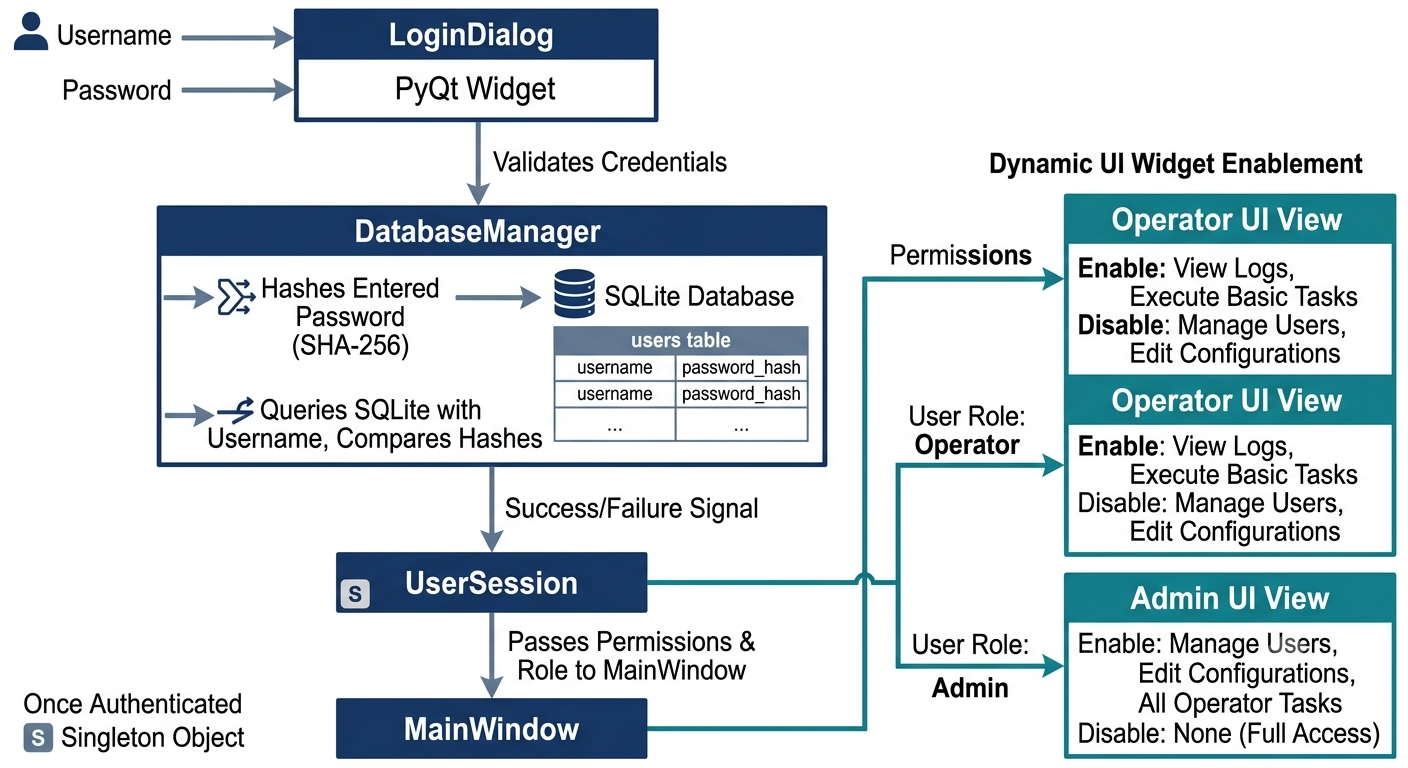
\includegraphics[width=0.95\linewidth]{img/pyqt_auth_architecture.png}
		\caption{معماری لایه‌ای احراز هویت و نحوه کنترل ویجت‌های PyQt بر اساس UserSession (تولید شده توسط هوش مصنوعی)}
		\label{fig:pyqt_auth}
	\end{figure}
	
	
	\subsection{لایه‌های ورودی داده: شبیه‌سازی \lr{Webots} و جریان ویدئویی (\lr{Data Input Pipelines})}
	
	یک سیستم ممیزی و کنترل کیفی هوشمند نیازمند لایه‌های ورودی چندگانه (\lr{Multi-source Input Pipelines}) جهت دریافت داده‌های تصویری و داده‌های حسگری (\lr{Telemetry Data}) به صورت بلادرنگ است. نرم‌افزار پیاده‌سازی‌شده دو خط‌لوله (پایپ‌لاین) ورودی مجزا اما هماهنگ را پشتیبانی می‌کند: لایه دریافت داده از محیط شبیه‌سازی خط تولید صنعتی در **\lr{Webots}** و لایه پردازش جریان تصویری از دوربین‌های محلی یا فایل‌های ویدئویی ضبط‌شده.
	
	\subsubsection{ورودی محیط شبیه‌سازی ویبات (\lr{Webots Simulation Integration})}
	جهت اعتبارسنجی و تست الگوریتم‌های کنترل سایبر-فیزیکی و بینایی در شرایط نزدیک به واقعیت، محیط شبیه‌ساز صنعتی \lr{Webots} به نرم‌افزار متصل شده است. تعامل سیستم با شبیه‌ساز از طریق کدهای مستقر در پوشه‌های \lr{\texttt{webots/}} و \lr{\texttt{simulation/}} مدیریت می‌شود:
	
	\begin{enumerate}
		\item \textbf{معماری ارتباطی و کنترلر کانوایر (\lr{\texttt{webots/}}):} 
		کدهای موجود در پوشه \lr{\texttt{webots/}} به عنوان کنترلر نیتیو (\lr{Native Controller}) در درون شبیه‌ساز اجرا می‌شوند. این ماژول‌ها وظیفه دریافت فرامینی نظیر تغییر سرعت موتور نوار نقاله (\lr{Conveyor Belt}) یا توقف اضطراری از سوی لایه کنترل پایتون (\lr{\texttt{controllers/}}) و اعمال مستقیم آن‌ها به عملگرهای فیزیکی شبیه‌ساز را بر عهده دارند.
		
		\item \textbf{مدیریت نشست شبیه‌سازی (\lr{\texttt{simulation/}}):} 
		ماژول‌های این لایه وظیفه بسترسازی ارتباطی میان نرم‌افزار اصلی و محیط شبیه‌ساز را بر عهده دارند. این ارتباط بر پایه سوکت‌های شبکه محلی (\lr{IPC / Socket Communication}) یا پروتکل‌های پیام‌رسانی سریع پیاده‌سازی شده است تا تأخیر انتقال داده‌ها به حداقل برسد.
		
		\item \textbf{استخراج بلادرنگ داده‌های تلمتری (\lr{Real-time Telemetry Extraction}):} 
		در هر گام زمانی (\lr{Time Step}) از شبیه‌سازی، داده‌های حسگری به صورت متناوب استخراج و به نرم‌افزار ارسال می‌شوند:
		\begin{itemize}
			\item \textbf{سرعت لحظه‌ای کانوایر:} مقدار واقعی سرعت خط بر حسب متر بر ثانیه ($m/s$).
			\item \textbf{موقعیت مکانی قطعات:} مختصات سه بعدی ($X, Y, Z$) قطعات نوردشده روی نوار نقاله جهت ارزیابی فاصله و سرعت نسبی.
			\item \textbf{سیگنال‌های انکودر و سنسورهای موقعیت:} ثبت متغیرهای حالت برای ورودی به عامل یادگیری تقویتی (\lr{RL}) و ناظر فازی.
		\end{itemize}
	\end{enumerate}
	
	\subsubsection{ورودی از فایل‌های ویدئویی و دوربین محلی (\lr{Video Stream Input Processing})}
	لایه پردازش بینایی نرم‌افزار نیازمند جریان پیوسته و بدون وقفه فریم‌های تصویری است. این لایه به‌گونه‌ای طراحی شده است که بتواند هم از فایل‌های ویدئویی تست (فرمت‌های \lr{MP4/AVI}) و هم از دوربین‌های صنعتی محلی (\lr{USB / RTSP IP Cameras}) ورودی دریافت کند.
	
	\begin{itemize}
		\item \textbf{ماژول بارگذاری و رمزگشایی فریم‌ها (\lr{Frame Ingestion}):} 
		با استفاده از کتابخانه \lr{OpenCV} در لایه پردازش، ورودی تصویری باز شده و فریم‌ها به صورت ماتریس‌های \lr{NumPy} استخراج می‌شوند. برای جلوگیری از افت فریم در خروجی تصویری، نمونه‌برداری فریم‌ها بر اساس نرخ فریم واقعی (\lr{FPS}) منبع تنظیم می‌گردد.
		
		\item \textbf{مدیریت صف فریم‌ها و حافظه میانگیر (\lr{Frame Buffering}):} 
		پردازش فریم‌ها توسط مدل‌های عمیق \lr{YOLO} ممکن است زمان‌بر باشد. برای جلوگیری از سرریز حافظه رم (\lr{RAM Overflow}) و مانع شدن از تأخیر انباشته (\lr{Latency Accumulation})، از یک صف با ظرفیت محدود (\lr{Thread-safe Bounded Queue}) استفاده شده است. در صورتی که سرعت پردازش از سرعت دریافت فریم کمتر شود، جدیدترین فریم به عنوان الگوی جایگزین انتخاب شده و فریم‌های قدیمی‌تر ریزش می‌کنند (\lr{Frame Dropping Strategy}) تا پایش همواره بلادرنگ باقی بماند.
		
		\item \textbf{اتصال به ماژول بینایی (\lr{\texttt{perception/}}):} 
		فریم‌های بازخوانی‌شده از صف میانگیر، مستقیماً به کلاس اصلی پردازش تصویر در پوشه \lr{\texttt{perception/}} متصل می‌شوند. در این ماژول، تغییر سایز فریم‌ها، تبدیل فضاهای رنگی و استنتاج مدل \lr{YOLO} انجام شده و تصاویر علامت‌گذاری‌شده (\lr{Annotated Frames}) جهت نمایش به رابط کاربری (\lr{\texttt{ui/}}) ارسال می‌گردند.
	\end{itemize}
	
	\begin{table}[htbp]
		\centering
		\caption{مقایسه ویژگی‌های عملیاتی دو لایه ورودی داده در نرم‌افزار}
		\label{tab:input_pipelines_comparison}
		\resizebox{\linewidth}{!}{
			\begin{tabular}{|l|l|l|l|}
				\hline
				\textbf{منبع ورودی} & \textbf{ماژول مربوطه در کد} & \textbf{نوع داده دریافتی} & \textbf{نرخ به‌روزرسانی / تأخیر} \\ \hline
				شبیه‌ساز \lr{Webots} & \lr{\texttt{webots/} , \texttt{simulation/}} & تلمتری حرکتی + مختصات فیزیکی & همگام با گام شبیه‌سازی ($32ms$) \\ \hline
				دوربین زنده / فایل ویدئو & \lr{\texttt{perception/} , \texttt{ui/}} & فریم‌های تصویری RGB & $30$ فریم بر ثانیه / کمتر از $15ms$ \\ \hline
			\end{tabular}
		}
	\end{table}
	
	\begin{figure}[htbp]
		\centering
		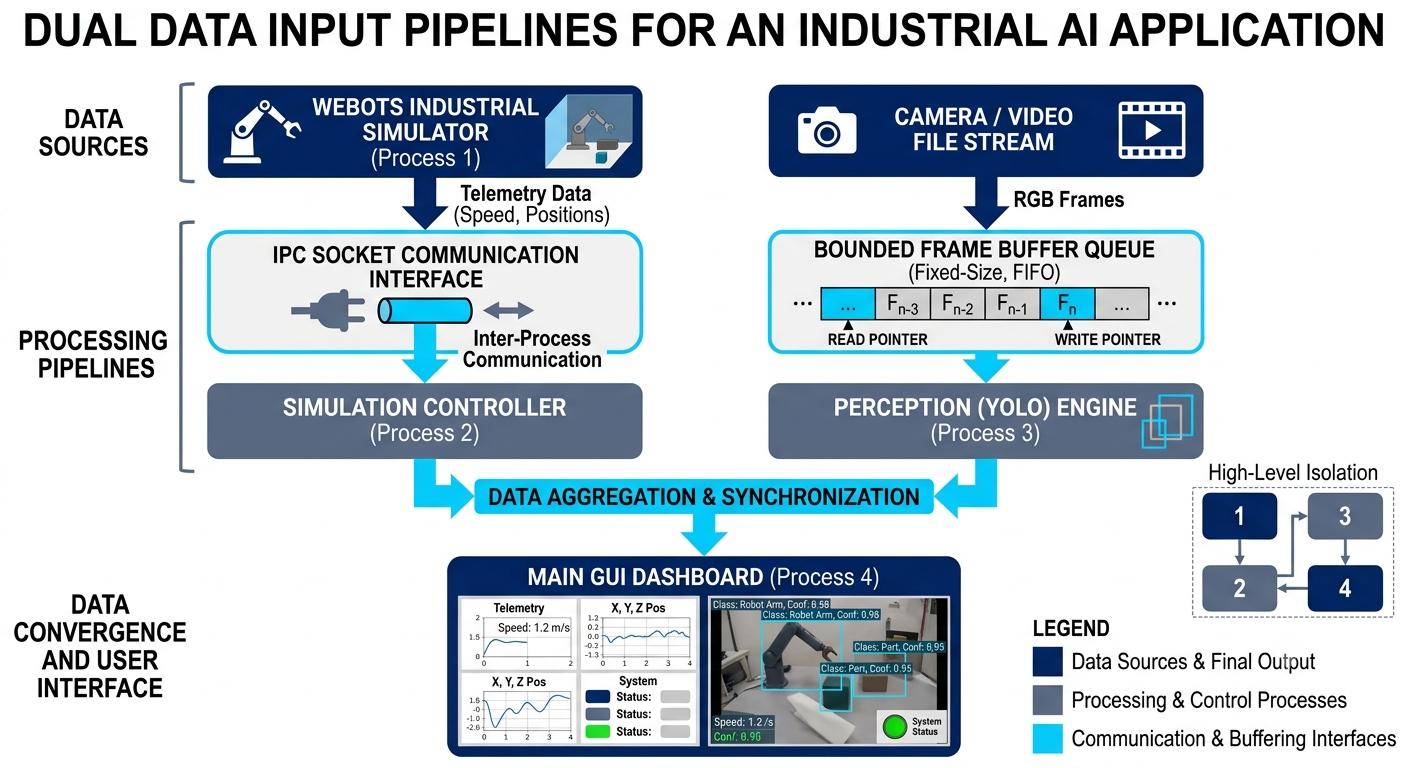
\includegraphics[width=0.95\linewidth]{img/data_input_pipelines.png}
		\caption{معماری پایپ‌لاین ورودی داده‌ها از محیط شبیه‌سازی Webots و جریان ویدئویی به ماژول‌های پردازشی نرم‌افزار (تولید شده توسط هوش مصنوعی)}
		\label{fig:input_pipelines}
	\end{figure}
	
	\subsection{ماژول تولید گزارش و هوش مصنوعی (\lr{Automated Reporting \& SLM Integration})}
	
	ارزیابی داده‌های عددی و تلمتری در محیط‌های صنعتی سنگین، نیازمند ترجمه این متغیرها به گزارش‌های کیفی و روایی قابل فهم برای اپراتوران و مدیران کیفی است. ماژول گزارش‌گیری خودکار در این نرم‌افزار، وظیفه برقراری ارتباط میان داده‌های خام حاصل از لایه بینایی (\lr{YOLO}) و سیستم کنترل سایبر-فیزیکی (\lr{RL/Fuzzy}) با مدل زبانی کوچک محلی (\lr{SLM}) را بر عهده دارد. کدهای این بخش به صورت یکپارچه در پوشه \lr{\texttt{reporting/}} سازمان‌دهی شده‌اند.
	
	\subsubsection{ساختار و وظایف ماژول گزارش‌گیری (\lr{\texttt{reporting/}})}
	ماژول موجود در پوشه \lr{\texttt{reporting/}} به عنوان پل ارتباطی بین لایه‌های محاسباتی سنگین و لایه تولید متن عمل می‌کند. وظایف محوری کدهای این بخش به شرح زیر است:
	
	\begin{enumerate}
		\item \textbf{استخراج و تجمیع داده‌ها (\lr{Data Aggregation}):} جمع‌آوری شاخص‌های کلیدی عملکرد (\lr{KPIs}) شامل درصد قطعیت مانیتورینگ بینایی، کلاس‌های عیب شناسایی‌شده، نوسانات سرعت کانوایر، خروجی‌های عامل یادگیری تقویتی و درجه ریسک تعیین‌شده توسط سیستم فازی در طی یک پنجره زمانی مشخص.
		\item \textbf{ساختاردهی استاندارد ورودی (\lr{JSON Serialization}):} تبدیل داده‌های متغیر و پراکنده فیزیکی به یک شیء منسجم و نفوذناپذیر در قالب \lr{JSON}. این ساختاردهی مانع از سردرگمی مدل زبانی و ورود اطلاعات اشتباه می‌شود.
		\item \textbf{ساخت پرامپت پویا (\lr{Dynamic Prompt Construction}):} تزریق داده‌های \lr{JSON} استخراج‌شده به قالب پرامپت سیستمی پیش‌فرض که شامل دستورالعمل‌های سخت‌گیرانه نگارشی، ساختار ۵ بخشی گزارش و الزامات عدم توهم است.
	\end{enumerate}
	
	\subsubsection{اتصال لایه استنتاج محلی به نرم‌افزار و فراخوانی مدل \lr{Qwen}}
	برای حفظ حریم خصوصی داده‌های صنعتی و حذف تأخیر ناشی از ارتباطات ابری، استنتاج مدل زبانی به صورت ۱۰۰٪ محلی در لایه لبه انجام می‌گیرد. اتصال نرم‌افزار پایتون به موتور استنتاج مدل زبانی سری \lr{Qwen-2.5} طی فرآیند زیر مدیریت می‌شود:
	
	\begin{itemize}
		\item \textbf{استفاده از کتابخانه‌های استنتاج محلی (\lr{Inference Engines}):} فراخوانی مدل زبانی از طریق رابط‌های برنامه‌نویسی پایتون مانند کتابخانه \lr{\texttt{ollama-python}} یا سرویس‌های محلی \lr{REST API} خادم \lr{vLLM} انجام می‌پذیرد.
		\item \textbf{تنظیم دقیق ابرپارامترهای استنتاج در کد:} جهت تضمین قطعیت و رفتار یکنواخت خروجی، پارامترهای استنتاج به صورت نرم‌افزاری در زمان ارسال درخواست تنظیم می‌شوند:
		\begin{equation}
			T = 0.05, \quad Top\text{-}P = 0.1, \quad Frequency\_Penalty = 1.15, \quad Max\_Tokens = 350
		\end{equation}
		\item \textbf{مدیریت پاسخ غیرهمگام (\lr{Asynchronous Execution}):} فراخوانی مدل زبانی به دلیل ماهیت پردازشی آن، در یک نخ جداگانه (\lr{Worker Thread}) اجرا می‌شود تا رابط کاربری \lr{PyQt} در زمان استنتاج قفل یا کاملاً بلوک نشود.
	\end{itemize}
	
	\subsubsection{فرمت‌دهی، ذخیره‌سازی و خروجی‌گرفتن از گزارش‌ها}
	پس از دريافت متن روایی فارسی از مدل زبانی محلی، ماژول \lr{\texttt{reporting/}} عملیات پس‌پردازش و ثبت خروجی را طی سه گانه زیر تکمیل می‌کند:
	
	\begin{enumerate}
		\item \textbf{اعتبارسنجی و پاک‌سازی خروجی (\lr{Output Post-processing}):} بررسی متن خروجی جهت اطمینان از وجود ۵ بخش کلیدی گزارش و حذف هرگونه کاراکتر زاید یا توکن‌های توقف ناخواسته.
		\item \textbf{ذخیره‌سازی همزمان در پایگاه داده (\lr{Database Persistence}):} ثبت متن کامل گزارش تولیدشده در جدول \lr{\texttt{generated\_reports}} دیتابیس \lr{SQLite} همراه با شناسه نشست جاری (\lr{Session ID}) و برچسب زمانی (\lr{Timestamp}) دقیق.
		\item \textbf{تولید خروجی استاندارد (\lr{PDF / Text Export}):} فراهم نمودن امکان استخراج گزارش‌ها در قالب فایل‌های متنی (\lr{.txt}) یا سندهای ساختاریافته \lr{PDF} با پشتیبانی کامل از فونت‌های فارسی و لوگوی رسمی کارخانه جهت ارائه به مدیران ارشد کیفیت.
	\end{enumerate}
	
	\begin{table}[htbp]
		\centering
		\caption{جریان نگاشت داده‌ها از لایه محاسباتی به گزارش نهایی در ماژول reporting}
		\label{tab:reporting_pipeline}
		\resizebox{\linewidth}{!}{
			\begin{tabular}{|l|l|l|}
				\hline
				\textbf{مرحله پردازشی} & \textbf{فرمت داده} & \textbf{مولفه اجرایی در کد} \\ \hline
				تجمّع داده‌های سنسورها و بینایی & داده‌های متغیر پایتون (\lr{Dict/NumPy}) & \lr{reporting.data\_collector} \\ \hline
				ساختاردهی ورودی & رشته استاندارد \lr{JSON} & \lr{reporting.prompt\_builder} \\ \hline
				استنتاج هوش مصنوعی محلی & متن خام فارسی (\lr{Raw String}) & \lr{reporting.slm\_client (Qwen-2.5)} \\ \hline
				پست‌پروسس و خروجی‌گیری & فایل \lr{PDF / Database Record} & \lr{reporting.exporter \& data.database} \\ \hline
			\end{tabular}
		}
	\end{table}
	
	\subsection{طراحی رابط کاربری و تعاملات گرافیکی (\lr{User Interface Architecture with PyQt})}
	
	در سامانه‌های مانیتورینگ و کنترل کیفی صنعتی بلادرنگ، رابط کاربری (\lr{User Interface - UI}) فراتر از یک لایه بصری ساده است؛ این لایه به عنوان داشبورد عملیاتی اپراتور و مرکز تصمیم‌گیری لحظه‌ای عمل می‌کند. چالش اصلی در طراحی این لایه، حفظ روانی و نرخ به‌روزرسانی بالای رابط کاربری (حداقل ۳۰ فریم بر ثانیه) همزمان با دریافت و پردازش حجم عظیمی از داده‌های تصویری، محاسبات فازی/یادگیری تقویتی و استنتاج سنگین مدل‌های زبانی محلی است.
	
	\subsubsection{چرایی انتخاب فریم‌ورک \lr{PyQt / PySide}}
	برای پیاده‌سازی لایه گرافیکی نرم‌افزار، فریم‌ورک **\lr{PyQt}** (مبتنی بر کتابخانه قدرتمند \lr{Qt} در \lr{C++}) انتخاب گردید. دلایل فنی و مهندسی این انتخاب به شرح زیر است:
	
	\begin{itemize}
		\item \textbf{کارایی بالا در رندرینگ بلادرنگ (\lr{High-Performance Rendering}):} استفاده از شتاب‌دهنده گرافیکی سخت‌افزاری و قابلیت تبدیل بهینه‌سازی‌شده فریم‌های تصویری (\lr{NumPy Arrays}) به اشیای بصری \lr{QImage/QPixmap}، نمایش بدون تأخیر تصاویر دوربین را تضمین می‌کند.
		\item \textbf{پشتیبانی بومی از معماری چندنخی (\lr{Native Multithreading Support}):} برخلاف کتابخانه‌های گرافیکی ساده‌تر پایتون (نظیر \lr{Tkinter})، \lr{PyQt} کلاس‌های پیشرفته‌ای مانند \lr{\texttt{QThread}} را ارائه می‌دهد که امکان اجرای وظایف سنگین پردازشی را در پس‌زمینه بدون مسدودسازی نخ اصلی فراهم می‌سازد.
		\item \textbf{انعطاف‌پذیری در شخصی‌سازی (\lr{Custom Widget Styling}):} قابلیت اعمال شیوه‌نامه‌های سفارشی (\lr{QSS - Qt Style Sheets}) جهت بومی‌سازی کامل محیط کاربر و طراحی تم‌های صنعتی کم‌نور (\lr{Dark Mode}) برای کاهش خستگی چشم اپراتور در اتاق‌های کنترل.
	\end{itemize}
	
	\subsubsection{ساختار معماری کد در پوشه \lr{\texttt{ui/}}}
	کدهای لایه گرافیکی به صورت کاملاً مدولار در پوشه \lr{\texttt{ui/}} سازمان‌دهی شده‌اند. این تفکیک ماژولار اجازه می‌دهد هر بخش از رابط کاربری مسئولیت مستقلی را بر عهده داشته باشد:
	
	\begin{itemize}
		\item \textbf{پنجره اصلی (\lr{\texttt{MainWindow}}):} المان مرکزی برنامه که مدیریت تب‌های اصلی (مانیتورینگ زنده، تحلیل گزارش‌ها و تنظیمات)، منوهای بالایی، نوار وضعیت (\lr{StatusBar}) و نوار ابزار را بر عهده دارد.
		\item \textbf{کامپوننت نمایش زنده (\lr{\texttt{LiveStreamWidget}}):} ویجت اختصاصی جهت دریافت فریم‌های پردازش‌شده از لایه بینایی (\lr{\texttt{perception/}}). این کامپوننت فریم‌های دارای کادرهای احاطه‌کننده (\lr{YOLO Bounding Boxes})، برچسب کلاس‌های عیب و ضرایب اطمینان را به صورت بلادرنگ رندر می‌کند.
		\item \textbf{کامپوننت نمودارهای آنلاین (\lr{\texttt{AnalyticsChartWidget}}):} ترسیم دینامیک و لحظه‌ای تغییرات سرعت نوار نقاله، آمار تجمع عیوب سطحی و سطح عدم قطعیت مانیتورینگ با استفاده از ماژول‌های نمودارگیری سریع (مانند \lr{PyQtGraph / Matplotlib}).
		\item \textbf{پنل نمایش گزارش‌های \lr{SLM} (\lr{\texttt{ReportViewPanel}}):} بخش اختصاصی نمایش گزارش‌های تحلیلی فارسی تولیدشده توسط مدل زبانی محلی. این پنل به همراه نشانگرهای بصری وضعیت ایمنی (رنگ‌های سبز، زرد و قرمز برای سطوح ریسک خط) طراحی شده است.
	\end{itemize}
	
	\subsubsection{مدیریت همزمانی و نخ‌های پس‌زمینه (\lr{Multithreading with QThread})}
	عملیات پردازش تصویر سنگین، استنتاج مدل زبانی \lr{Qwen} و دریافت تلمتری از \lr{Webots}، در صورت اجرا روی نخ اصلی گرافیکی (\lr{Main GUI Thread}) موجب قفل شدن رابط کاربری (\lr{UI Freezing}) می‌شوند. برای حل این مشکل، یک معماری چندنخی پیشرفته پیاده‌سازی شده است.
	
	\begin{figure}[htbp]
		\centering
		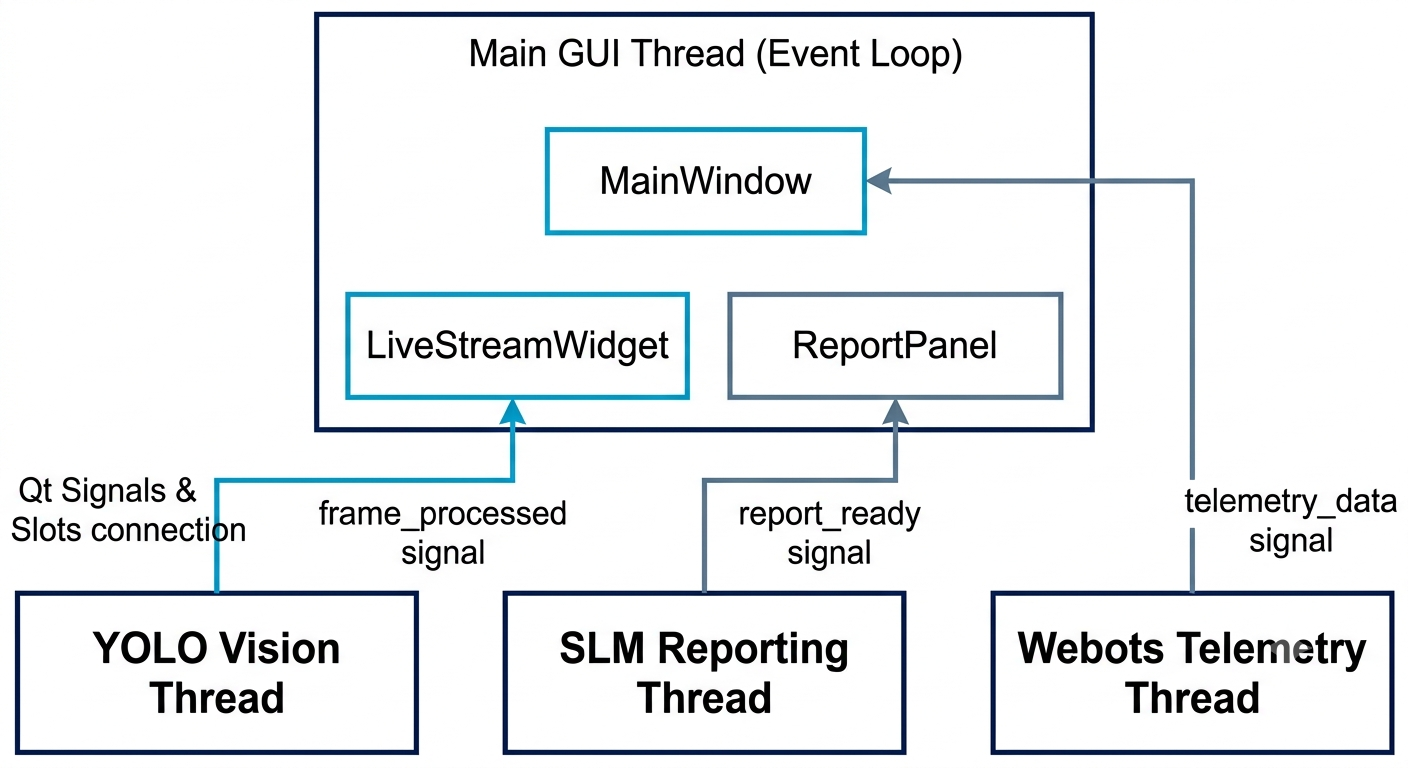
\includegraphics[width=0.95\linewidth]{img/pyqt_multithreading_architecture.png}
		\caption{معماری چندنخی PyQt، جداسازی نخ GUI از پردازش‌های سنگین و مکانیزم تعامل ایمن با Signals \& Slots (تولید شده توسط هوش مصنوعی)}
		\label{fig:pyqt_multithreading}
	\end{figure}
	
	در این معماری، نخ اصلی برنامه‌ کاربردی صرفاً وظیفه دریافت رویدادها (\lr{Event Loop}) و رندرینگ المان‌های بصری را بر عهده دارد. پردازش‌های سنگین به نخ‌های مجزا هدایت شده‌اند:
	\begin{enumerate}
		\item \textbf{نخ پردازش بینایی (\lr{YOLO Worker Thread}):} دریافت فریم خام، اجرای مدل \lr{YOLO} و ارسال فریم علامت‌گذاری‌شده به ویجت نمایش زنده.
		\item \textbf{نخ استنتاج زبانی (\lr{SLM Reporting Thread}):} ارسال درخواست به مدل زبانی، مدیریت زمان استنتاج چندثانیه‌ای و تحویل متن نهایی به پنل گزارش‌ها.
		\item \textbf{نخ شبیه‌ساز و تلمتری (\lr{Simulation Stream Thread}):} برقراری ارتباط مداوم با سوکت‌های \lr{Webots} و به‌روزرسانی متغیرهای حالت به صورت متناوب.
	\end{enumerate}
	
	\textbf{مکانیزم سیگنال و اسلات (\lr{Signals \& Slots}):} جهت برقراری ارتباط ایمن بین نخ‌های پس‌زمینه و نخ اصلی گرافیکی (که از نظر ایمنی نخ یا \lr{Thread-Safety} حساس است)، تمامی داده‌ها (مانند فریم جدید، متون گزارش و داد‌ه‌های تلمتری) از طریق **سیگنال‌های سفارشی \lr{PyQt}** منتقل می‌شوند. این مکانیزم تضمین می‌کند که هیچ دسترسی مستقیمی از نخ‌های پردازشی به ویجت‌های گرافیکی صورت نگرفته و مانع از بروز خطاهای بحرانی (\lr{Segmentation Faults}) گردد.
	
	\begin{table}[htbp]
		\centering
		\caption{تفکیک نخ‌ها (Threads) و سیگنال‌های ارتباطی در معماری رابط کاربری PyQt}
		\label{tab:pyqt_threads}
		\resizebox{\linewidth}{!}{
			\begin{tabular}{|l|l|l|l|}
				\hline
				\textbf{عنوان نخ (\lr{Thread})} & \textbf{ماژول اجرایی} & \textbf{سیگنال ارسالی (\lr{Signal})} & \textbf{اسلات دریافت‌کننده در \lr{UI}} \\ \hline
				\lr{Main GUI Thread} & \lr{ui.main\_window} & رویدادهای کاربر (\lr{Click/TabChange}) & به‌روزرسانی المان‌های دیداری \\ \hline
				\lr{YOLO Thread} & \lr{perception.yolo\_engine} & \lr{frame\_processed(QImage)} & \lr{LiveStreamWidget.update\_frame} \\ \hline
				\lr{SLM Thread} & \lr{reporting.slm\_worker} & \lr{report\_ready(QString)} & \lr{ReportViewPanel.display\_text} \\ \hline
				\lr{Telemetry Thread} & \lr{simulation.webots\_client} & \lr{telemetry\_data(dict)} & \lr{AnalyticsChartWidget.add\_point} \\ \hline
			\end{tabular}
		}
	\end{table}
	
	\subsection{پیکربندی، تنظیمات و دارایی‌ها (\lr{Configuration \& Assets Management})}
	
	نرم‌افزارهای صنعتی مانیتورینگ برای تضمین انطباق‌پذیری (\lr{Adaptability}) و نگهداری‌پذیری (\lr{Maintainability})، نباید وابسته به مقادیر سخت‌کدشده (\lr{Hardcoded Values}) در متن برنامه باشند. هرگونه تغییر در آستانه‌های تشخیص هوش مصنوعی، مسیر وزن مدل‌ها یا المان‌های دیداری رابط کاربری باید بدون نیاز به دستکاری کدهای سورس و بازکمپایل برنامه صورت پذیرد. بدین منظور، لایه مدیریت پیکربندی و دارایی‌های گرافیکی نرم‌افزار به صورت کاملاً مجزا در پوشه‌های \lr{\texttt{config/}} و \lr{\texttt{assets/}} پیاده‌سازی شده است.
	
	\subsubsection{مدیریت تنظیمات نرم‌افزار (\lr{\texttt{config/}})}
	تمامی متغیرهای عملیاتی، آستانه‌های ریسک و تنظیمات لایه استنتاج هوش مصنوعی در پوشه \lr{\texttt{config/}} و در قالب فایل‌های ساختاریافته \lr{YAML} یا \lr{JSON} نگهداری می‌شوند. ماژول لودر پیکربندی (\lr{\texttt{config/loader.py}}) در زمان راه‌اندازی برنامه (\lr{Startup}) این متغیرها را بارگذاری کرده و در اختیار ماژول‌های مربوطه قرار می‌دهد.
	
	\begin{itemize}
		\item \textbf{تنظیمات مدل زبانی محلی (\lr{SLM Parameters}):} تنظیم متغیرهایی نظیر دمای استنتاج ($T = 0.05$)، پارامتر $Top\text{-}P = 0.1$، جریمه‌های تکرار ($Frequency\_Penalty = 1.15$)، حداکثر طول توکن‌ها ($Max\_Tokens = 350$) و آدرس \lr{API} خادم محلی.
		\item \textbf{آستانه‌های لایه بینایی و کنترل کیفیت (\lr{Vision \& Control Thresholds}):} تعریف مسیر فایل وزن‌های آموزش‌دیده مدل \lr{YOLO}، آستانه ضریب اطمینان (\lr{Confidence Threshold}) جهت ثبت عیوب و آستانه‌های تعیین سطح ریسک در ناظر فازی.
		\item \textbf{تنظیمات سخت‌افزاری و دیتابیس (\lr{System \& Database Configs}):} نگهداری آدرس درگاه‌های ارتباطی با شبیه‌ساز \lr{Webots}، نرخ فریم مطلوب دوربین‌ها و مسیر ذخیره‌سازی فایل پایگاه داده \lr{SQLite}.
	\end{itemize}
	
	\begin{table}[htbp]
		\centering
		\caption{ساختار نمونه فایل پیکربندی نرم‌افزار جهت پارامتردهی دینامیک}
		\label{tab:config_structure}
		\resizebox{\linewidth}{!}{
			\begin{tabular}{|l|l|l|}
				\hline
				\textbf{بخش پیکربندی (\lr{Section})} & \textbf{کلید نمونه (\lr{Key})} & \textbf{مقدار پیش‌فرض / نقش مهندسی} \\ \hline
				\lr{slm\_config} & \lr{temperature} & \lr{0.05} (کنترل قطعیت خروجی مدل زبانی) \\ \hline
				\lr{vision\_config} & \lr{weights\_path} & \lr{"models/yolo\_defect.pt"} (مسیر فایل وزن‌ها) \\ \hline
				\lr{control\_config} & \lr{fuzzy\_risk\_threshold} & \lr{0.75} (آستانه فعال‌سازی هشدار خطر) \\ \hline
				\lr{database\_config} & \lr{db\_file\_path} & \lr{"data/monitoring.db"} (مسیر فایل دیتابیس) \\ \hline
			\end{tabular}
		}
	\end{table}
	
	\subsubsection{مدیریت منابع گرافیکی و تم‌های دیداری (\lr{\texttt{assets/}})}
	پوشه \lr{\texttt{assets/}} مسئولیت متمرکزسازی تمامی منابع دیداری، آیکون‌ها و استایل‌شیت‌های رابط کاربری را بر عهده دارد. این جداسازی تضمین می‌کند که رابط گرافیکی نرم‌افزار کاملاً منعطف و قابل برندسازی باشد:
	
	\begin{enumerate}
		\item \textbf{استایل‌شیت‌های سفارشی (\lr{QSS - Qt Style Sheets}):} تعریف فایل‌های \lr{.qss} جهت اعمال تم‌های دیداری تاریک صنعتی (\lr{Dark Industrial Theme}). این استایل‌ها فونت‌های فارسی، رنگ‌بندی دکمه‌های کنترلی، وضعیت‌های هشدار و جداول را به صورت یکپارچه در تمامی ویجت‌های \lr{PyQt} تنظیم می‌کنند.
		\item \textbf{مدیریت آیکون‌ها و لوگوها (\lr{Icons \& Images}):} ذخیره‌سازی تمامی آیکون‌های وکتوری (فرمت‌های \lr{SVG/PNG}) مربوط به وضعیت دکمه‌ها (مانند کلید توقف اضطراری، ضبط ویدیو، تنظیمات) و لوگوی رسمی کارخانه جهت درج در لایه‌بندی گزارش‌های \lr{PDF} استخراج‌شده.
	\end{enumerate}
	
	
	معماری جداسازی پیکربندی و دارایی‌ها باعث می‌شود تا بدون اصلاح کدهای سورس پایتون، توانایی کالیبراسیون دقیق سیستم، تغییر آستانه‌ها در محیط‌های صنعتی مختلف و شخصی‌سازی ظاهر برنامه به راحتی فراهم گردد.
	% دستور چاپ رفرنس‌ها
	\newpage
	
	
	\begin{LTR}
		\printbibliography[title={\rl{Refrences}}]
	\end{LTR}
	
\end{document}